%============================================================
%  Deep Learning – Note di Studio
%  Politecnico di Bari – Prof. Vito Walter Anelli
%  Compatibile con Overleaf (pdflatex)
%============================================================
\documentclass[12pt, a4paper]{report}

% --- Encoding e lingua ---
\usepackage[T1]{fontenc}
\usepackage[utf8]{inputenc}
\usepackage[provide=*,italian]{babel}

% --- Layout ---
\usepackage[top=2.5cm, bottom=2.5cm, left=3cm, right=2.5cm]{geometry}
\setlength{\parskip}{4pt}
\setlength{\parindent}{1.2em}

% --- Matematica ---
\usepackage{amsmath, amssymb, mathtools}
\usepackage{bm}
\newtheorem{theorem}{Teorema}[chapter]

% --- Grafica ---
\usepackage{graphicx}
\usepackage{float}

% --- Tabelle ---
\usepackage{booktabs}
\usepackage{array}
\usepackage{tabularx}
\usepackage{adjustbox}

% --- Colori e link ---
\usepackage{xcolor}
\usepackage[colorlinks=true, linkcolor=blue!60!black,
            citecolor=green!50!black, urlcolor=blue]{hyperref}

% --- Liste ---
\usepackage{enumitem}
\setlist{itemsep=2pt, topsep=4pt}

% --- Intestazioni ---
\usepackage{fancyhdr}
\pagestyle{fancy}
\fancyhf{}
\fancyhead[L]{\small\itshape Deep Learning}
\fancyhead[R]{\small\itshape\nouppercase{\leftmark}}
\fancyfoot[C]{\thepage}
\renewcommand{\headrulewidth}{0.4pt}

% --- Codice ---
\usepackage{listings}
\lstset{
  basicstyle=\ttfamily\small,
  backgroundcolor=\color{gray!10},
  frame=single, rulecolor=\color{gray!40},
  breaklines=true,
  keywordstyle=\color{blue!70!black}\bfseries,
  commentstyle=\color{green!50!black},
  stringstyle=\color{red!60!black},
  numbers=left, numberstyle=\tiny\color{gray},
}

% --- Ambienti semplici ---
\usepackage{tcolorbox}
\tcbuselibrary{skins, breakable}

\newenvironment{definizione}[1][]{%
  \par\smallskip\noindent
  \textbf{Definizione\ifx&#1&\else\ (#1)\fi.}\quad\itshape
}{\par\smallskip}

\newenvironment{osservazione}{%
  \par\smallskip\noindent
  \textbf{Osservazione.}\quad
}{\par\smallskip}

\newenvironment{attenzione}{%
  \par\smallskip\noindent
  \textbf{Attenzione.}\quad\itshape
}{\par\smallskip}

% --- Riferimenti bibliografici ---
\usepackage[round, authoryear, sort]{natbib}
\newcommand{\parencite}[1]{\citep{#1}}

% --- Comandi matematici ---
\newcommand{\vect}[1]{\boldsymbol{#1}}
\newcommand{\matr}[1]{\boldsymbol{#1}}
\newcommand{\R}{\mathbb{R}}
\newcommand{\pd}[2]{\frac{\partial #1}{\partial #2}}
\newcommand{\norm}[1]{\left\lVert #1 \right\rVert}
\DeclareMathOperator{\softmax}{softmax}
\DeclareMathOperator{\relu}{ReLU}

% --- Riferimenti alle fonti ---
\newcommand{\refbishop}[1]{\textsuperscript{[B\,#1]}}
\newcommand{\reflecun}[1]{\textsuperscript{[NYU\,#1]}}

%============================================================
\begin{document}

% --- Frontespizio ---
\begin{titlepage}
  \centering
  \vspace*{2cm}
  {\LARGE\bfseries Deep Learning}\\[0.5cm]
  {\large Note di Studio}\\[1.5cm]
  {\normalsize Basato sulle slide del Prof.\ \textbf{Vito Walter Anelli}\\
  Politecnico di Bari -- SisInf Lab}\\[1cm]
\end{titlepage}

% --- Prefazione ---
\chapter*{Prefazione}
\addcontentsline{toc}{chapter}{Prefazione}

Queste note sono redatte come supporto allo studio del corso di
\textbf{Deep Learning} del Prof.\ Vito Walter Anelli (Politecnico di Bari).
Il testo integra le slide ufficiali del corso con due risorse fondamentali:
\textit{NYU-DLSP21} \citep{lecun2021} di LeCun e Canziani e
\textit{Deep Learning: Foundations and Concepts} \citep{bishop2024}
di Bishop \& Bishop.

Nel testo, le etichette \textsuperscript{[B\,X]} rimandano al capitolo X del
libro Bishop, mentre \textsuperscript{[NYU\,Y]} alla settimana Y del corso NYU.

% --- Indice ---
\tableofcontents
\newpage

%============================================================
% CAPITOLI
%============================================================
%============================================================
%  Capitolo 0 – Introduzione al Deep Learning
%============================================================
\chapter{Introduzione al Deep Learning}
\label{ch:intro}

La veloce crescita odierna del Machine Learning ha portato alla nascita di nuove
tecnologie e campi di applicazione. Il \textbf{Deep Learning} nasce con
l'intento di apprendere rappresentazioni gerarchiche direttamente dai dati,
tramite reti neurali profonde. I campi di applicazione spaziano dalla
diagnostica medica fino ai Large Language Models (LLM) \citep{bishop2024}.

%------------------------------------------------------------
\section{Machine Learning vs Deep Learning}
\label{sec:ml-vs-dl}

Nel \textbf{Machine Learning classico} la pipeline si divide in due fasi
nettamente separate: un'estrazione di feature progettata manualmente
dall'ingegnere, seguita da un classificatore appreso automaticamente dai dati.
Nel \textbf{Deep Learning} entrambe le fasi sono apprese congiuntamente e in
modo gerarchico: i layer bassi catturano edge e texture, quelli intermedi parti
di oggetti, quelli alti concetti semantici \citep{lecun2021}.

\begin{figure}[H]
  \centering
  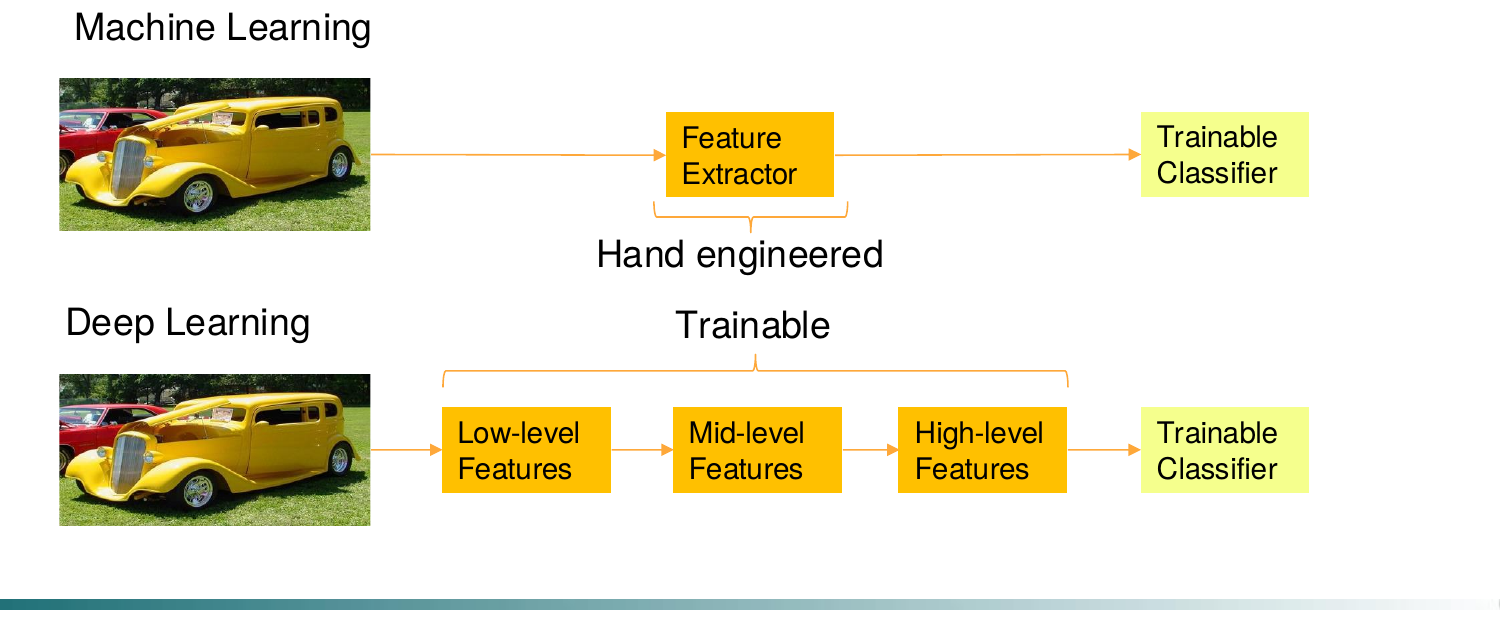
\includegraphics[width=0.88\linewidth]{figures/ml_vs_dl.png}
  \caption{Confronto tra la pipeline di ML classico (feature extractor
           hand-engineered + classificatore) e quella di Deep Learning
           (tutta la catena è trainable end-to-end).}
  \label{fig:ml_vs_dl}
\end{figure}

Il Deep Learning si colloca all'interno della gerarchia
\textit{AI} $\supset$ \textit{Machine Learning} $\supset$
\textit{Representation Learning} $\supset$ \textit{Deep Learning}.
La figura seguente mostra questa gerarchia e il corrispondente spettro
di paradigmi, dal rule-based al deep learning.

\begin{figure}[H]
  \centering
  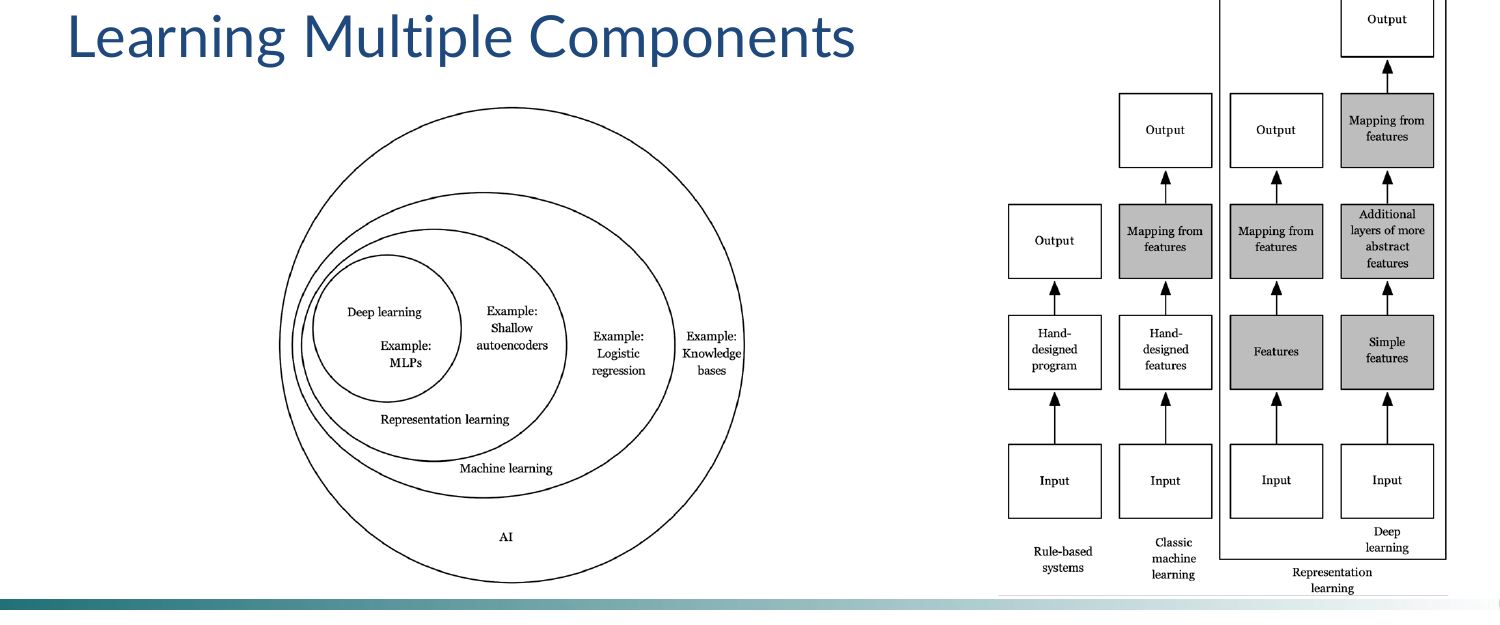
\includegraphics[width=0.92\linewidth]{figures/learning_components.png}
  \caption{Gerarchia AI/ML/Repr.\,Learning/DL (sinistra) e i quattro
           paradigmi principali con il loro grado di automazione (destra).}
  \label{fig:learning_components}
\end{figure}

Un esempio storico di benchmark è il dataset \textbf{MNIST} \citep{lecun1998}:
$70\,000$ immagini $28{\times}28$ pixel di cifre scritte a mano (0--9).
Un MLP semplice raggiunge circa il 98\% di accuratezza; la CNN LeNet-5 arriva
al 99.3\%.

%------------------------------------------------------------
\section{Modello Parametrico e Funzione di Costo}
\label{sec:parameterized-model}

Un \textbf{modello parametrico} è una funzione deterministica della forma
\begin{equation}
  \bar{y} = G(x,\, w)
\end{equation}
dove $x$ è l'ingresso osservato, $w$ il vettore dei parametri addestrabili
e $\bar{y}$ l'uscita predetta. I parametri $w$ sono condivisi tra tutti i
campioni di addestramento, mentre $x$ varia da campione a campione.

\begin{figure}[H]
  \centering
  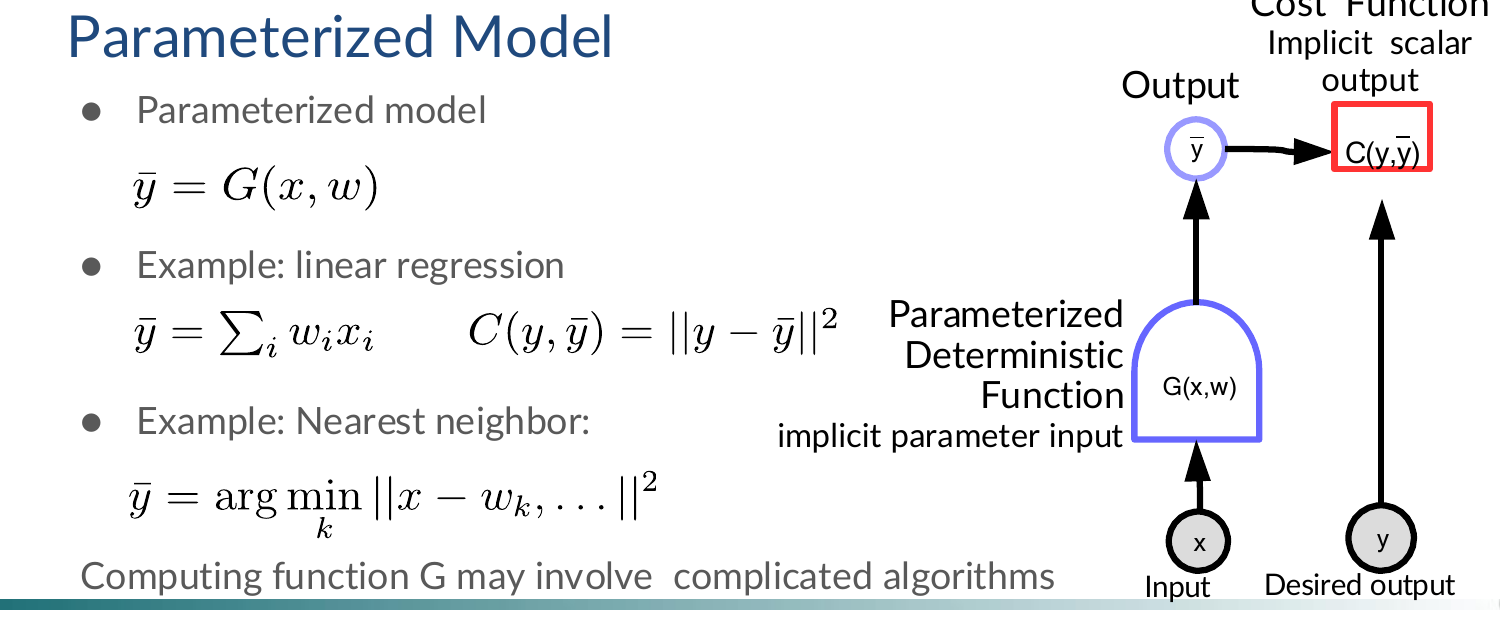
\includegraphics[width=0.88\linewidth]{figures/param_model.png}
  \caption{Schema del modello parametrico $\bar{y}=G(x,w)$. Il blocco
           $G(x,w)$ (rettangolo blu) prende in input $x$ e produce $\bar{y}$;
           la funzione di costo $C(y,\bar{y})$ (rettangolo rosso) ha output
           scalare implicito.}
  \label{fig:param_model}
\end{figure}

Due esempi fondamentali sono la \textbf{regressione lineare},
$\bar{y} = \sum_i w_i x_i$ con costo $C(y,\bar{y}) = \|y - \bar{y}\|^2$,
e il \textbf{k-Nearest Neighbor},
$\bar{y} = \arg\min_k \|x - w_{k,.}\|^2$,
dove i parametri $w_k$ coincidono con i prototipi del dataset di training.

\subsection{Notazione con grafi a blocchi}
\label{ssec:block-diagram}

Le slide del corso adottano una notazione grafica precisa per i grafi
computazionali \reflecun{W1}, illustrata nella figura seguente.

\begin{figure}[H]
  \centering
  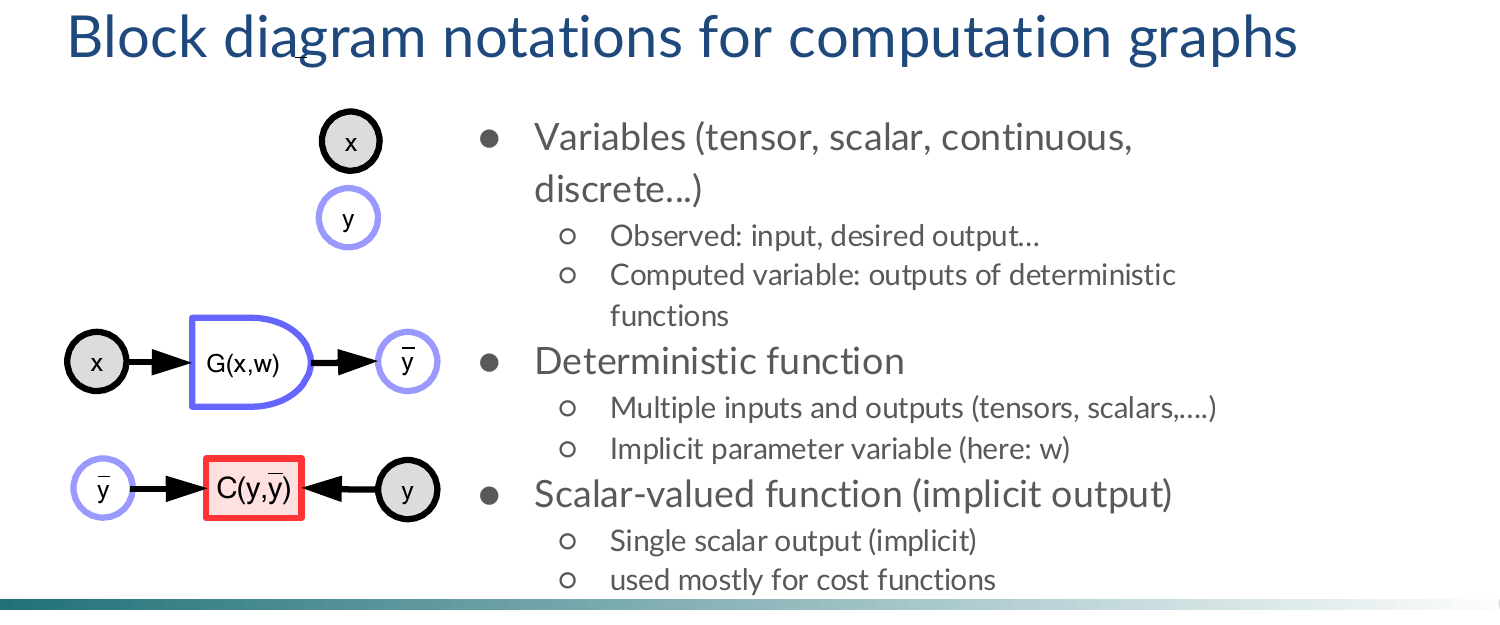
\includegraphics[width=0.82\linewidth]{figures/block_diagram.png}
  \caption{Notazione a blocchi per grafi computazionali: cerchi a bordo
           spesso = variabili osservate; cerchi a bordo sottile = variabili
           calcolate; rettangoli blu = funzioni deterministiche; rettangoli
           rossi = funzioni di costo con output scalare implicito.}
  \label{fig:block_diagram}
\end{figure}

\subsection{Funzione di loss e loss media}
\label{ssec:loss}

La \textbf{loss per campione} è $L(x, y, w) = C(y, G(x, w))$.
Dato il dataset $S = \{(x[p], y[p]) \mid p = 0, \ldots, P-1\}$,
la \textbf{loss media} è:
\begin{equation}
  \mathcal{L}(S,\, w)
  = \frac{1}{P}\sum_{p=0}^{P-1} L(x[p],\, y[p],\, w).
\end{equation}
L'obiettivo dell'apprendimento è $w^* = \arg\min_w \mathcal{L}(S,w)$.

\begin{figure}[H]
  \centering
  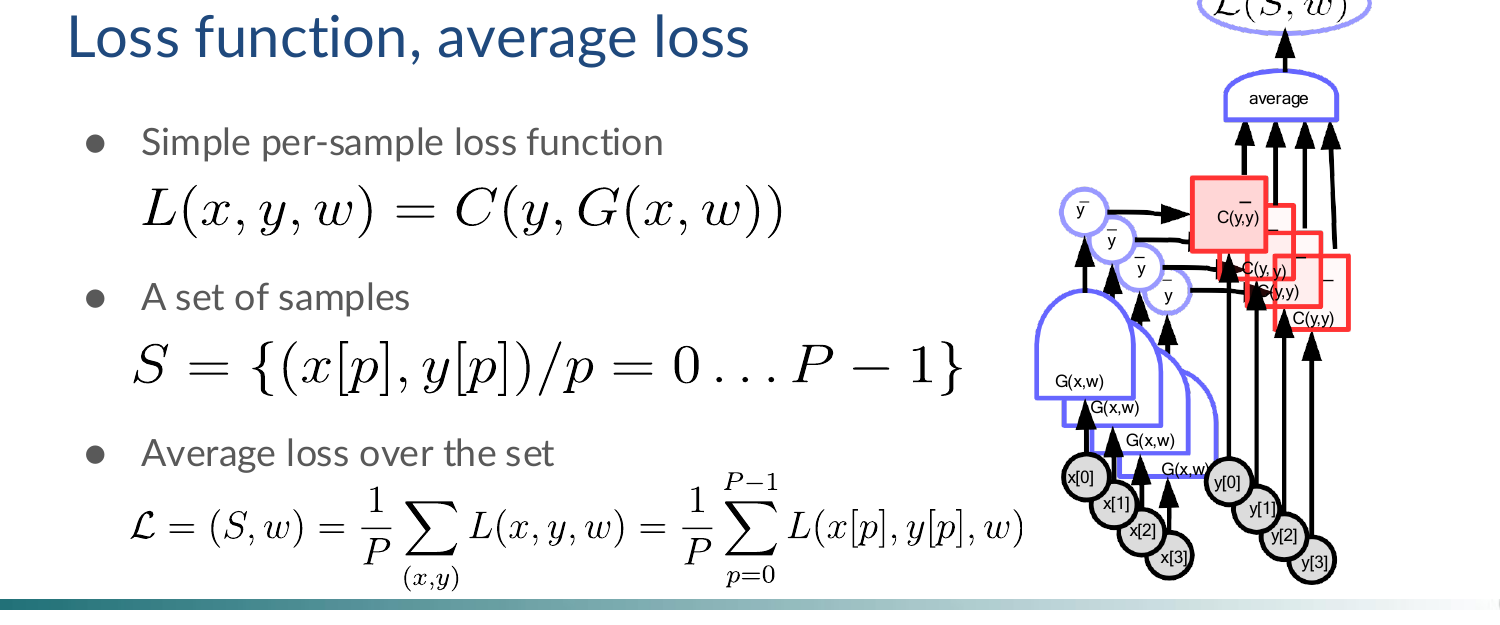
\includegraphics[width=0.88\linewidth]{figures/loss_avg.png}
  \caption{Grafo computazionale della loss media: il blocco $G(x,w)$ è
           replicato per ogni campione (con pesi condivisi) e le loss
           individuali $C(y,\bar{y})$ vengono mediate.}
  \label{fig:loss_avg}
\end{figure}

%------------------------------------------------------------
\section{Reti Neurali Tradizionali}
\label{sec:traditional-nn}

Una rete neurale tradizionale è una composizione alternata di blocchi
\textbf{lineari} e \textbf{non-lineari} \refbishop{6}:
\begin{align}
  s_{k+1} &= w_k\, z_k  \qquad &&\text{(blocco lineare)} \\
  z_k     &= h(s_k)             &&\text{(blocco non-lineare)}
\end{align}
dove $h(\cdot)$ è una funzione di attivazione punto per punto.
Per un neurone $i$, indicando con $UP(i)$ i neuroni del livello precedente:
\begin{equation}
  s[i] = \sum_{j \in UP(i)} w[i,j] \cdot z[j], \qquad z[i] = f(s[i]).
\end{equation}

\begin{figure}[H]
  \centering
  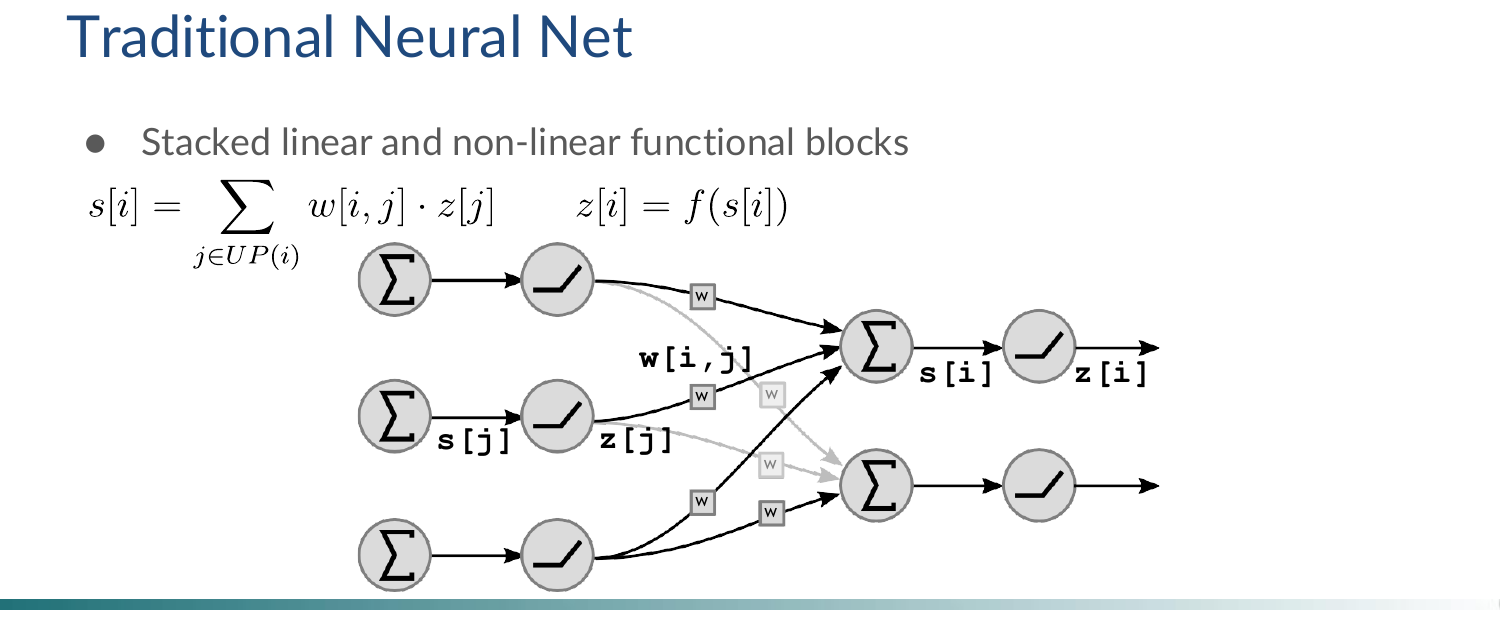
\includegraphics[width=0.88\linewidth]{figures/trad_nn.png}
  \caption{Struttura di una rete neurale tradizionale: i nodi $\Sigma$
           calcolano la somma pesata $s[i]$; i nodi con la curva applicano
           la non-linearità $z[i]=f(s[i])$; i riquadri $w$ rappresentano
           i pesi $w[i,j]$.}
  \label{fig:trad_nn}
\end{figure}

La catena lineare a blocchi per una rete a 3 layer è:
$x \xrightarrow{w_0} s_1 \xrightarrow{h} z_1 \xrightarrow{w_1} s_2
   \xrightarrow{h} z_2 \xrightarrow{w_2} s_3$.

\begin{figure}[H]
  \centering
  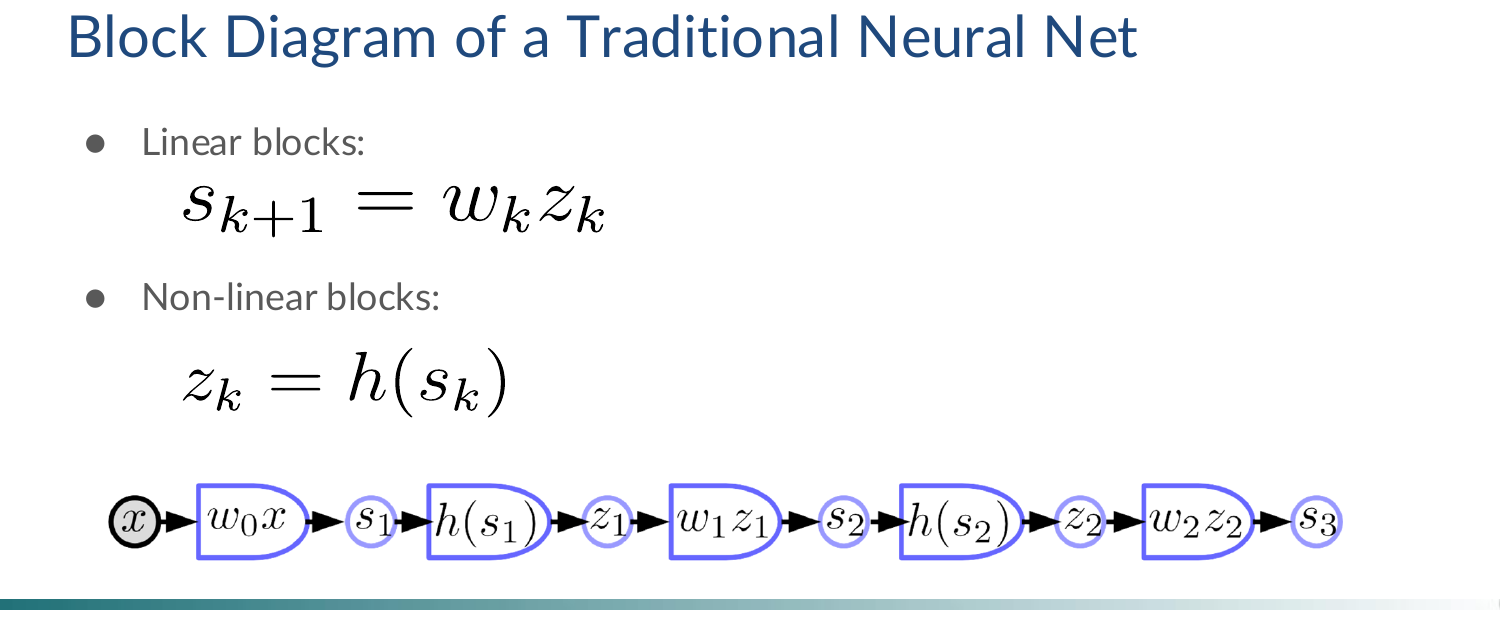
\includegraphics[width=0.88\linewidth]{figures/block_nn.png}
  \caption{Diagramma a blocchi di una rete a 3 layer: blocchi lineari
           (rettangoli) e non-lineari (forme arrotondate) si alternano.}
  \label{fig:block_nn}
\end{figure}

\subsection{Implementazione in PyTorch}

\begin{lstlisting}[language=Python, caption={MLP a 3 layer in PyTorch}]
import torch
from torch import nn

class MyNet(nn.Module):
    def __init__(self, d0, d1, d2, d3):
        super().__init__()
        self.m0 = nn.Linear(d0, d1)   # include bias
        self.m1 = nn.Linear(d1, d2)
        self.m2 = nn.Linear(d2, d3)

    def forward(self, x):
        z0 = x.view(-1)                # flatten
        z1 = torch.relu(self.m0(z0))
        z2 = torch.relu(self.m1(z1))
        return self.m2(z2)             # logit di output

model = MyNet(600, 60, 40, 10)
out   = model(torch.randn(3, 10, 20))
\end{lstlisting}

%------------------------------------------------------------
\section{Grafi Computazionali e Backpropagation}
\label{sec:backprop}

Un \textbf{grafo computazionale} è un DAG in cui i nodi foglia sono le variabili
di ingresso e i parametri, mentre i nodi interni rappresentano operazioni.
L'ordinamento topologico definisce l'ordine del forward e del backward pass
\refbishop{7}. Se il grafo contiene cicli (reti ricorrenti), è necessario
srotolarlo nel tempo (\textbf{BPTT}).

\subsection{Regola della catena -- caso scalare}

La backpropagation \citep{rumelhart1986} si fonda sulla \textbf{regola della
catena}: per $c = g(z)$, $z = h(s)$:
\begin{equation}
  \frac{dc}{ds} = \frac{dc}{dz} \cdot h'(s).
\end{equation}
Perturbando $s$ di $ds$ si perturba $z$ di $dz = h'(s)\,ds$, e quindi
$c$ di $dc = (dc/dz)\,dz$.

\begin{figure}[H]
  \centering
  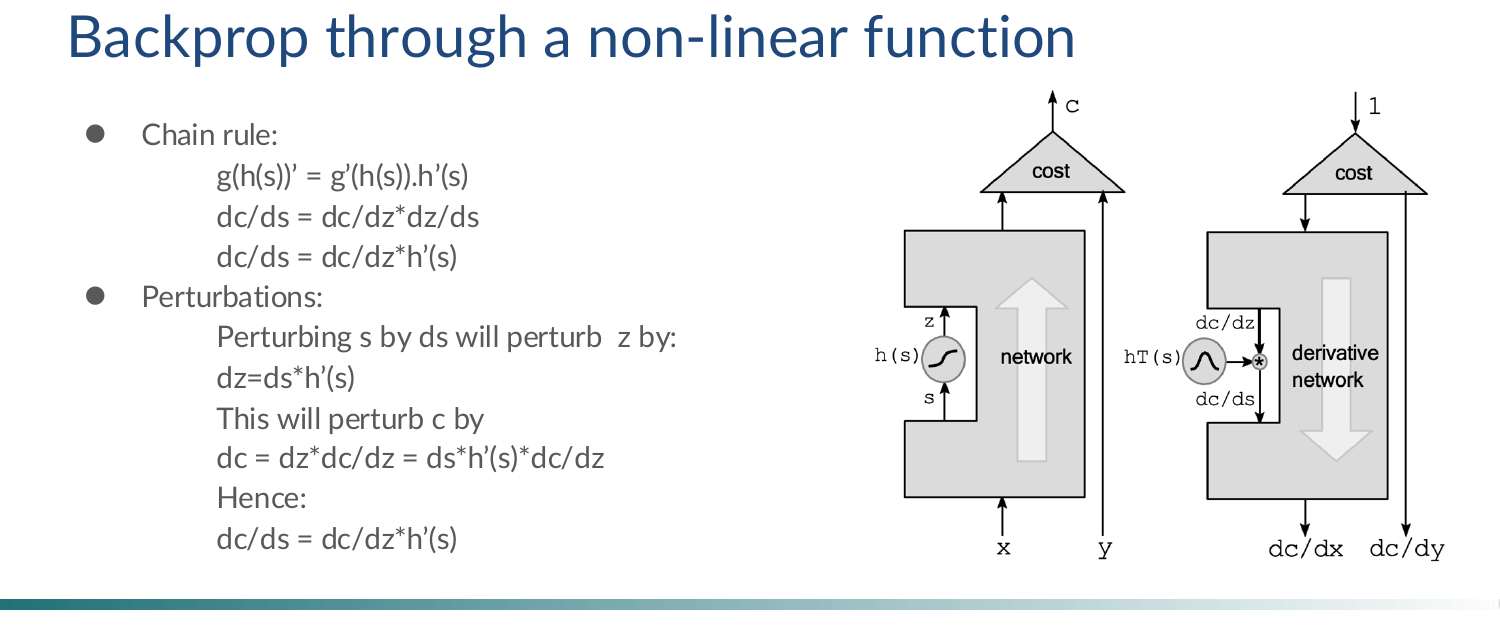
\includegraphics[width=0.82\linewidth]{figures/backprop_nonlin.png}
  \caption{Backprop attraverso una funzione non-lineare $h(s)$: la rete
           duale (destra) moltiplica il gradiente entrante $dc/dz$ per la
           derivata trasposta $h^T(s)$, producendo $dc/ds$.}
  \label{fig:backprop_nonlin}
\end{figure}

Per un neurone $z$ che alimenta più neuroni $s[0],s[1],s[2]$ tramite pesi
$w[0],w[1],w[2]$, il gradiente rispetto all'ingresso è la somma pesata:
\begin{equation}
  \frac{dc}{dz} = \sum_i \frac{dc}{ds[i]} \cdot w[i].
\end{equation}

\subsection{Caso vettoriale e matrice Jacobiana}

Per funzioni vettoriali con $z_f : [d_f \times 1]$ e $z_g : [d_g \times 1]$:
\begin{equation}
  \underbrace{\frac{\partial c}{\partial z_f}}_{[1 \times d_f]}
  = \underbrace{\frac{\partial c}{\partial z_g}}_{[1 \times d_g]}
    \cdot
    \underbrace{\frac{\partial z_g}{\partial z_f}}_{[d_g \times d_f]}.
\end{equation}
La \textbf{matrice Jacobiana} ha elemento $(i,j)$ uguale alla derivata
parziale della $i$-esima uscita rispetto alla $j$-esima entrata:
$(\partial z_g / \partial z_f)_{ij} = (\partial z_g)_i / (\partial z_f)_j$.

\begin{figure}[H]
  \centering
  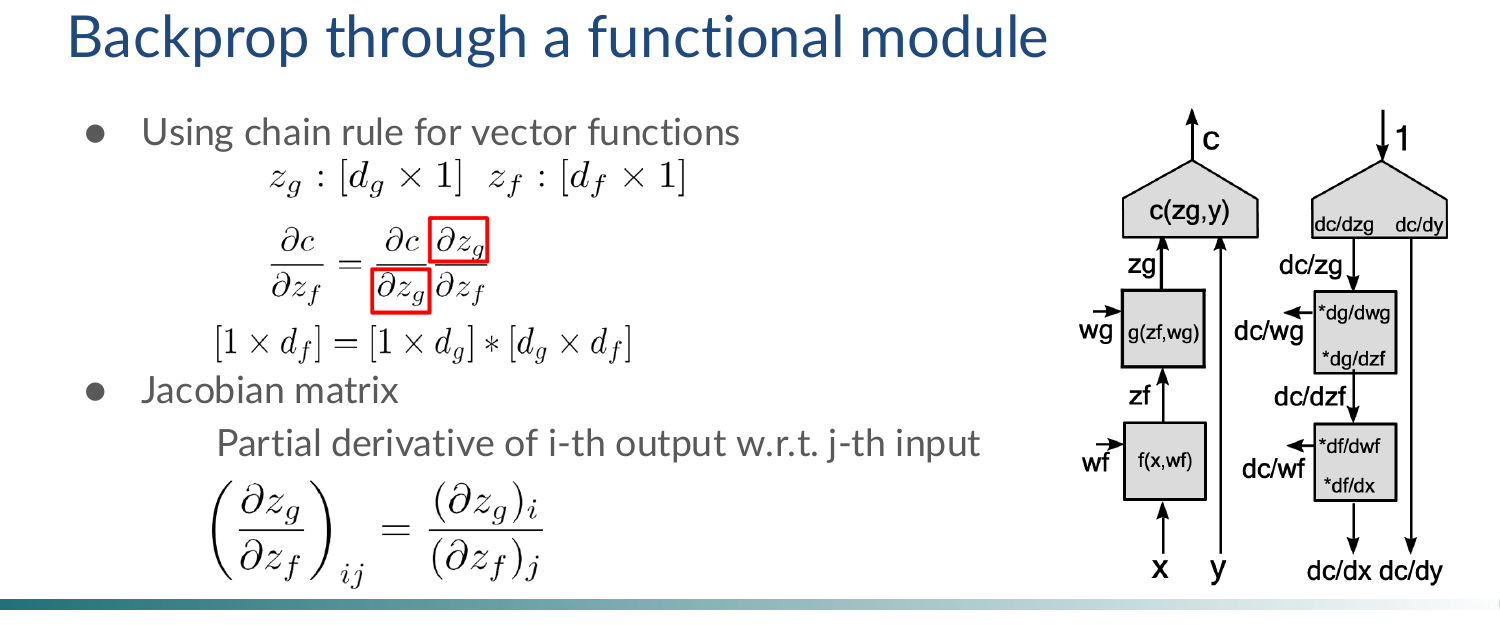
\includegraphics[width=0.88\linewidth]{figures/jacobian.png}
  \caption{Backprop attraverso un modulo vettoriale: ogni modulo espone
           due Jacobiane, una per i pesi ($*dg/dwg$) e una per l'ingresso
           ($*dg/dzf$), corrispondenti alle due frecce della rete duale.}
  \label{fig:jacobian}
\end{figure}

\subsection{Backprop in un grafo multi-stadio}

Per una rete a $K$ stadi con $z_{k+1} = f_k(z_k, w_k)$:
\begin{align}
  \frac{\partial c}{\partial z_k}
  &= \frac{\partial c}{\partial z_{k+1}}
     \cdot \frac{\partial f_k(z_k, w_k)}{\partial z_k}
  & &\text{(gradiente di stato)} \\
  \frac{\partial c}{\partial w_k}
  &= \frac{\partial c}{\partial z_{k+1}}
     \cdot \frac{\partial f_k(z_k, w_k)}{\partial w_k}
  & &\text{(gradiente dei pesi)}
\end{align}

\begin{figure}[H]
  \centering
  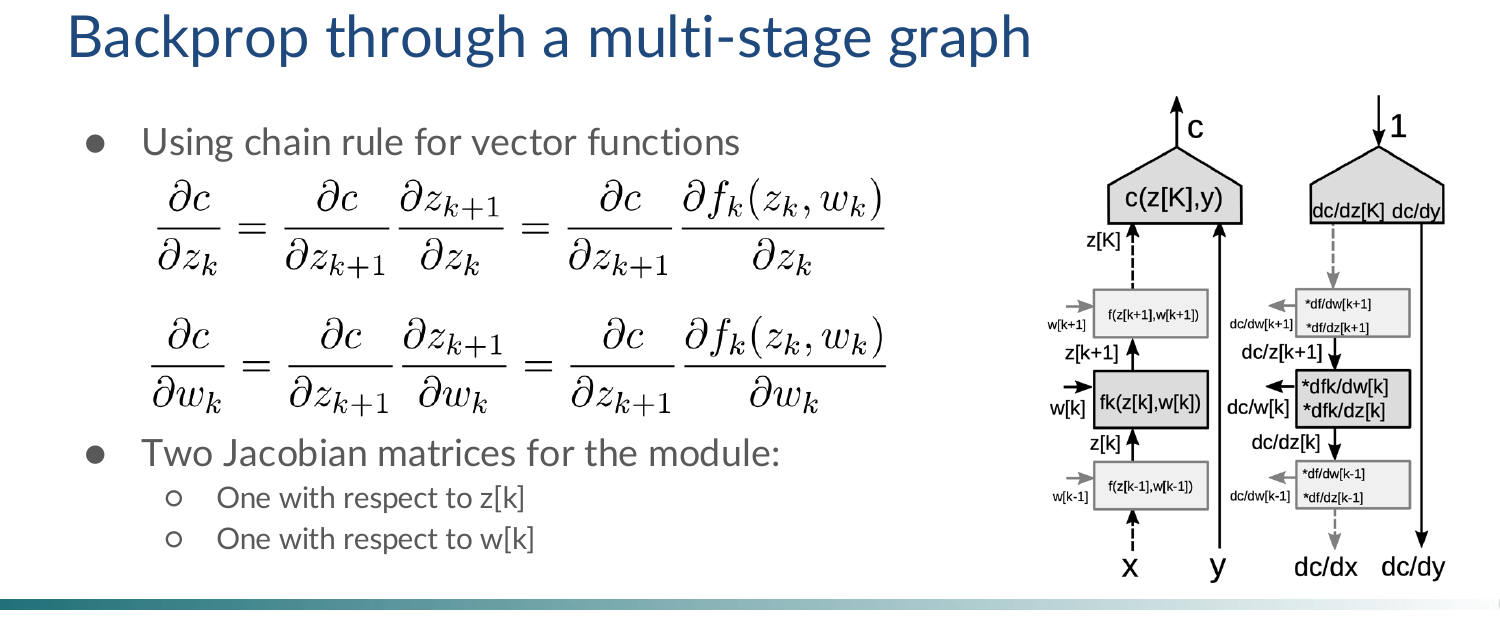
\includegraphics[width=0.88\linewidth]{figures/multistage.png}
  \caption{Backprop in un grafo multi-stadio: la rete duale (destra) esegue
           il forward pass ``al contrario'', con ogni modulo che produce due
           Jacobiane ($*dfk/dw[k]$ e $*dfk/dz[k]$).}
  \label{fig:multistage}
\end{figure}

La backpropagation è quindi una \textit{propagazione sul grafo duale}: ogni
nodo è sostituito dal suo modulo derivata, e il gradiente scende dall'output
verso l'input. Con $y,\bar{y}: [M\times1]$ e $w: [N\times1]$:
\begin{equation}
  \underbrace{\pd{C}{w}}_{[1\times N]}
  = \underbrace{\pd{C}{\bar{y}}}_{[1\times M]}
    \cdot
    \underbrace{\pd{\bar{y}}{w}}_{[M\times N]}.
\end{equation}

\begin{figure}[H]
  \centering
  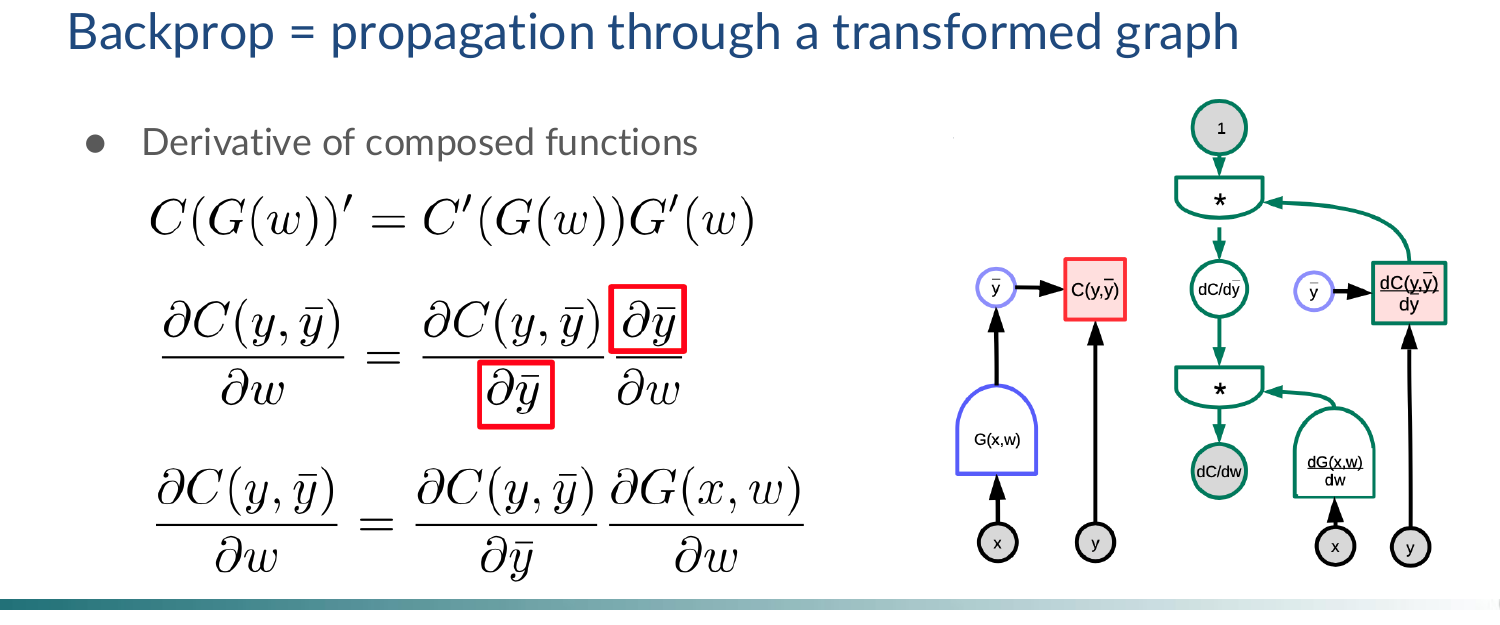
\includegraphics[width=0.82\linewidth]{figures/backprop_graph.png}
  \caption{Backprop come propagazione sul grafo duale: $\partial C/\partial w
           = (\partial C/\partial\bar{y})\cdot(\partial G/\partial w)$.}
  \label{fig:backprop_graph}
\end{figure}

La backpropagation è applicabile a qualsiasi DAG. Se il grafo ha cicli
(reti ricorrenti) occorre srotolarlo nel tempo (BPTT).

\begin{figure}[H]
  \centering
  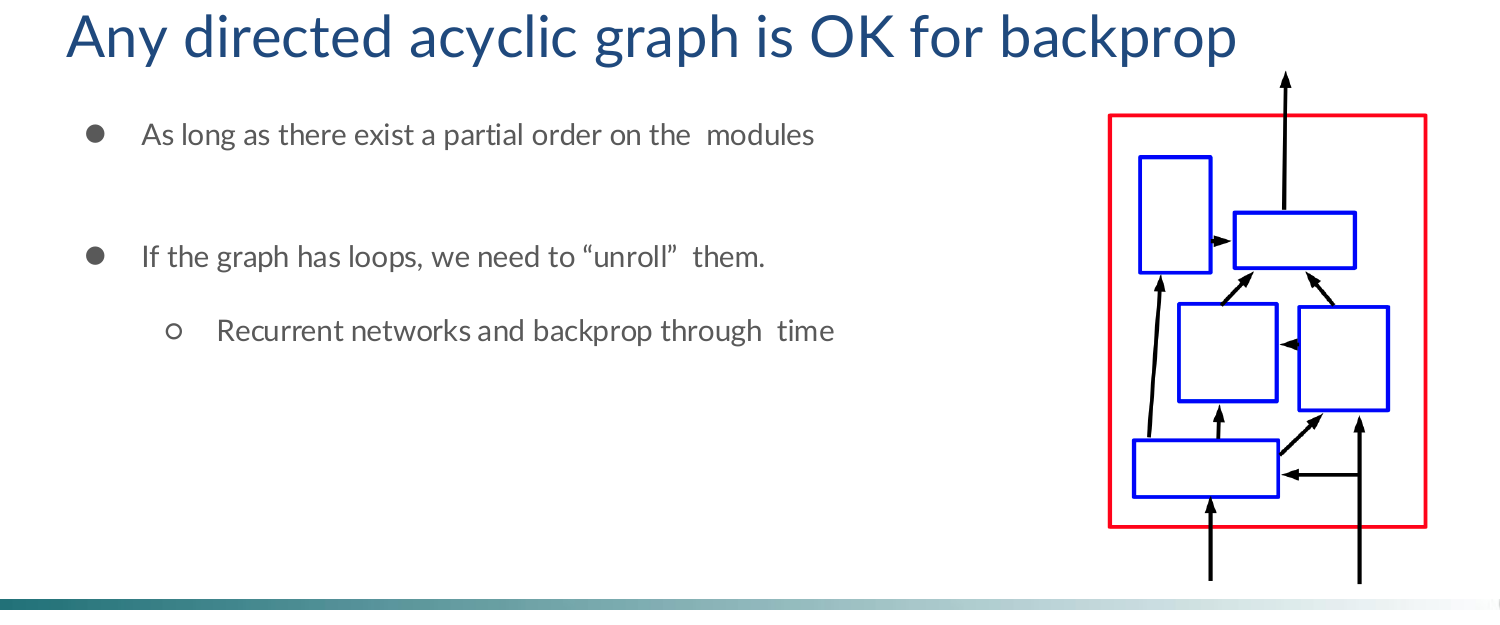
\includegraphics[width=0.55\linewidth]{figures/dag_backprop.png}
  \caption{Un esempio di DAG con flusso di dati in avanti (frecce nere) e
           backprop (frecce rosse) che lo percorre in senso inverso.}
  \label{fig:dag_backprop}
\end{figure}

%------------------------------------------------------------
\section{Riepilogo}
\label{sec:summary-ch0}

\begin{center}
\begin{tabular}{lll}
  \toprule
  \textbf{Concetto} & \textbf{Formula} & \textbf{Ruolo} \\
  \midrule
  Modello param.  & $\bar{y}=G(x,w)$                  & Base di ogni sistema ML \\
  Loss media      & $\mathcal{L}=\frac{1}{P}\sum_p C$  & Obiettivo \\
  Blocco lineare  & $s_{k+1}=w_k z_k$                  & Trasformazione affine \\
  Blocco non-lin. & $z_k=h(s_k)$                       & Capacità non-lineare \\
  Chain rule      & $dc/ds=(dc/dz)h'(s)$               & Motore backprop \\
  Jacobiano       & $(\partial z_g/\partial z_f)_{ij}$  & General.\ vettoriale \\
  DAG + backprop  & $\partial c/\partial z_k = \partial c/\partial z_{k+1}\cdot\partial f_k/\partial z_k$ & Algoritmo generale \\
  \bottomrule
\end{tabular}
\end{center}

%============================================================
%  Capitolo 1 – Architetture di Base
%============================================================
\chapter{Architetture di Base}
\label{ch:basic-arch}

Questo capitolo introduce i moduli fondamentali che estendono le reti neurali
standard con operazioni moltiplicative e meccanismi di condivisione dei
parametri. Questi concetti sono alla base di architetture moderne quali le reti
convoluzionali, i meccanismi di attenzione e i modelli Mixture of Experts
\citep{bishop2024, lecun2021}.

%------------------------------------------------------------
\section{Moduli Moltiplicativi}
\label{sec:multiplicative}

Le reti neurali classiche calcolano combinazioni lineari degli ingressi seguite
da una non-linearità. I \textbf{moduli moltiplicativi} generalizzano questa
idea permettendo che i pesi stessi dipendano da un secondo ingresso,
introducendo interazioni di ordine superiore tra feature.

\subsection{Unità Sigma-Pi e layer quadratico}

\begin{definizione}[Unità Sigma-Pi]
In una rete standard il pre-input è $s_i = \sum_j w_{ij}\, x_j$.
Nelle \textbf{unità Sigma-Pi} i pesi dipendono linearmente da un secondo
vettore di ingresso $\vect{z}$:
\begin{equation}
  w_{ij} = \sum_k u_{ijk}\, z_k
  \quad\Longrightarrow\quad
  s_i = \sum_{j,k} u_{ijk}\, z_k\, x_j
\end{equation}
dove $u_{ijk}$ sono i parametri effettivi del modello.
\end{definizione}

L'operazione è bilineare: lineare in $\vect{z}$ e in $\vect{x}$, ma quadratica
nel vettore congiunto $(\vect{z}, \vect{x})$. La figura seguente mostra il
diagramma computazionale dell'unità Sigma-Pi e, a destra, il modulo di
attenzione come caso speciale \refbishop{6}.

\begin{figure}[H]
  \centering
  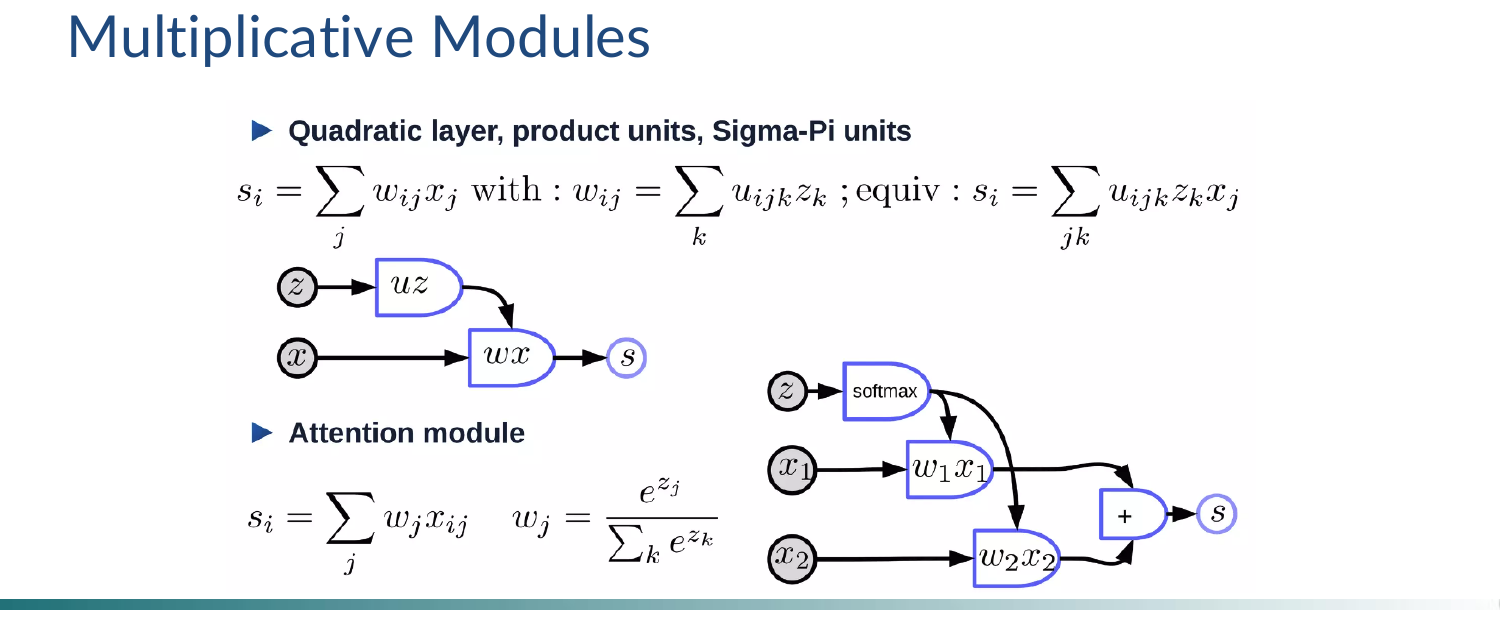
\includegraphics[width=0.88\linewidth]{figures/sigma_pi.png}
  \caption{Sinistra: unità Sigma-Pi -- il blocco $uz$ calcola i pesi dinamici
           da $z$, che vengono applicati all'ingresso $x$ nel blocco $wx$.
           Destra: modulo di attenzione -- $z$ passa per una softmax che
           produce i pesi $w_1, w_2$ per sommare le uscite pesate degli
           ingressi $x_1, x_2$.}
  \label{fig:sigma_pi}
\end{figure}

\subsection{Modulo di attenzione}

Il \textbf{meccanismo di attenzione} è il caso speciale in cui i pesi sono
normalizzati tramite softmax, formando una distribuzione di probabilità:
\begin{equation}
  s_i = \sum_j w_j\, x_{ij}, \qquad
  w_j = \frac{e^{z_j}}{\sum_k e^{z_k}} = \softmax(\vect{z})_j.
\end{equation}
La rete sceglie dinamicamente su quale ingresso concentrarsi in base al
contesto $\vect{z}$. Nel corso NYU \citep{lecun2021}, l'attenzione è
interpretata come un meccanismo di \textit{recupero soft} da una memoria
associativa, che anticipa direttamente l'architettura Transformer
\citep{vaswani2017}.

\subsection{Proprietà di differenziabilità}

Il modulo moltiplicativo con selezione discreta ($z_1 \in \{0,1\}$) non è
differenziabile rispetto ai parametri della porta di controllo, ma rimane
differenziabile rispetto a ingressi e uscite. La corrispondenza con la
selezione matriciale è:
\begin{equation}
  z_1{=}1,\,z_2{=}0:\;
  \begin{bmatrix}1&0\end{bmatrix}\!\begin{pmatrix}x_1\\x_2\end{pmatrix}=x_1,
  \quad
  z_1{=}0,\,z_2{=}1:\;
  \begin{bmatrix}0&1\end{bmatrix}\!\begin{pmatrix}x_1\\x_2\end{pmatrix}=x_2.
\end{equation}

\begin{figure}[H]
  \centering
  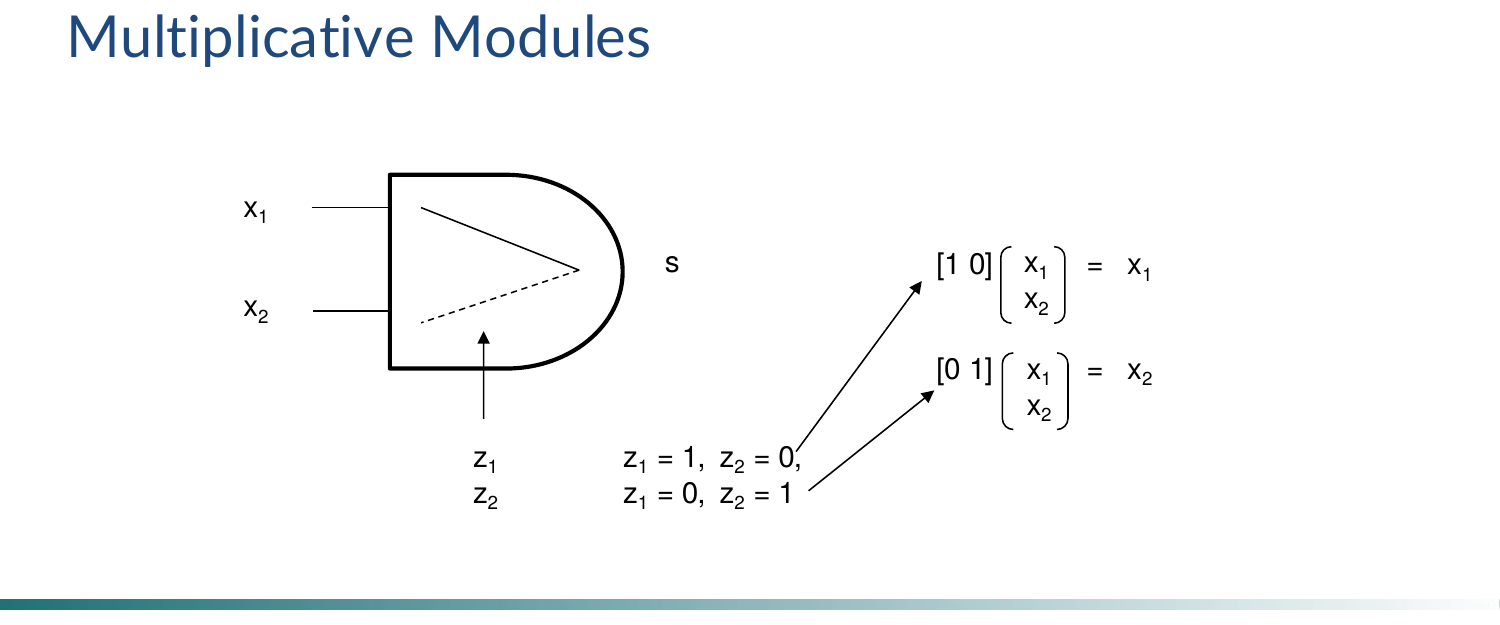
\includegraphics[width=0.72\linewidth]{figures/mux_discrete.png}
  \caption{Selezione discreta: quando $z_1=1, z_2=0$ il modulo seleziona
           $x_1$; quando $z_1=0, z_2=1$ seleziona $x_2$.}
  \label{fig:mux_discrete}
\end{figure}

\begin{figure}[H]
  \centering
  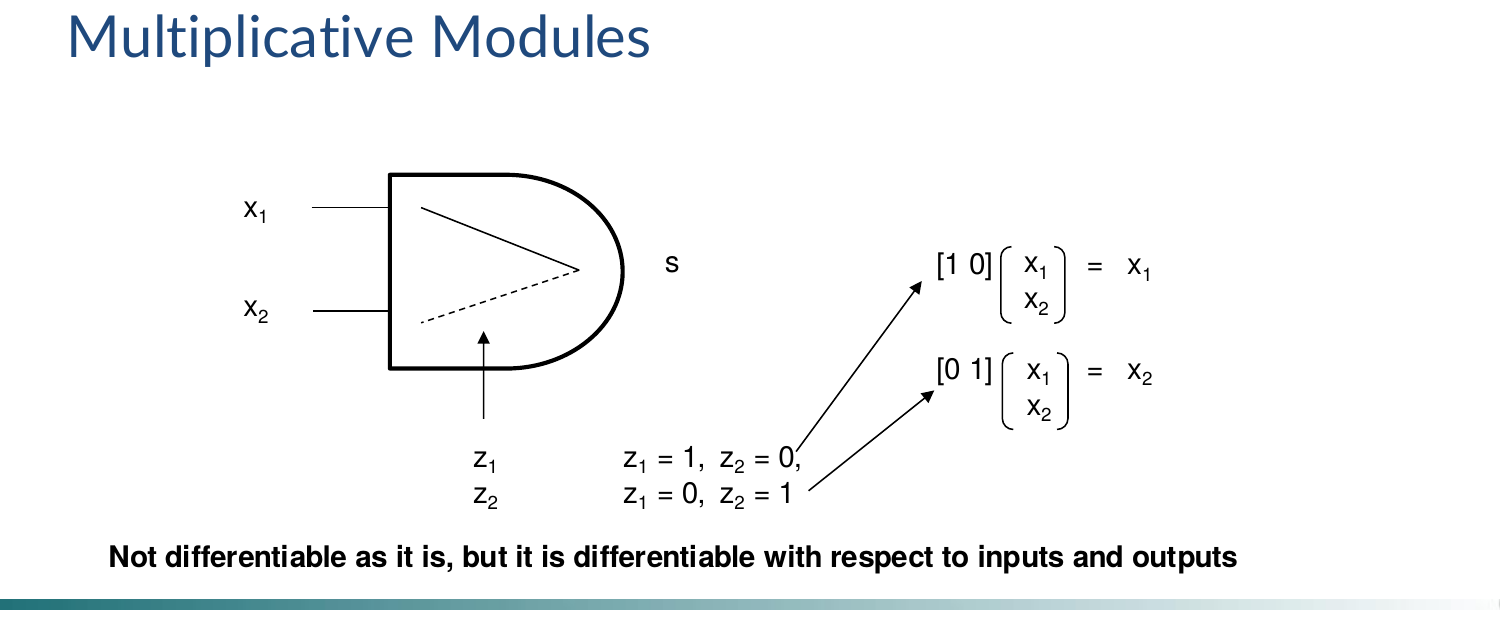
\includegraphics[width=0.72\linewidth]{figures/mux_diff.png}
  \caption{Il modulo con selezione discreta non è differenziabile come tale,
           ma lo è rispetto agli ingressi e alle uscite: il rilassamento
           tramite softmax rende tutto addestrabile con backpropagation.}
  \label{fig:mux_diff}
\end{figure}

%------------------------------------------------------------
\section{Mixture of Experts}
\label{sec:moe}

Il \textbf{Mixture of Experts} (MoE) generalizza il modulo di attenzione
applicandolo a intere reti esperto \citep{jacobs1991}:
\begin{equation}
  s_i = \sum_j w_j\, x_{ij}, \qquad
  w_j = \softmax(\vect{z})_j.
\end{equation}

\begin{figure}[H]
  \centering
  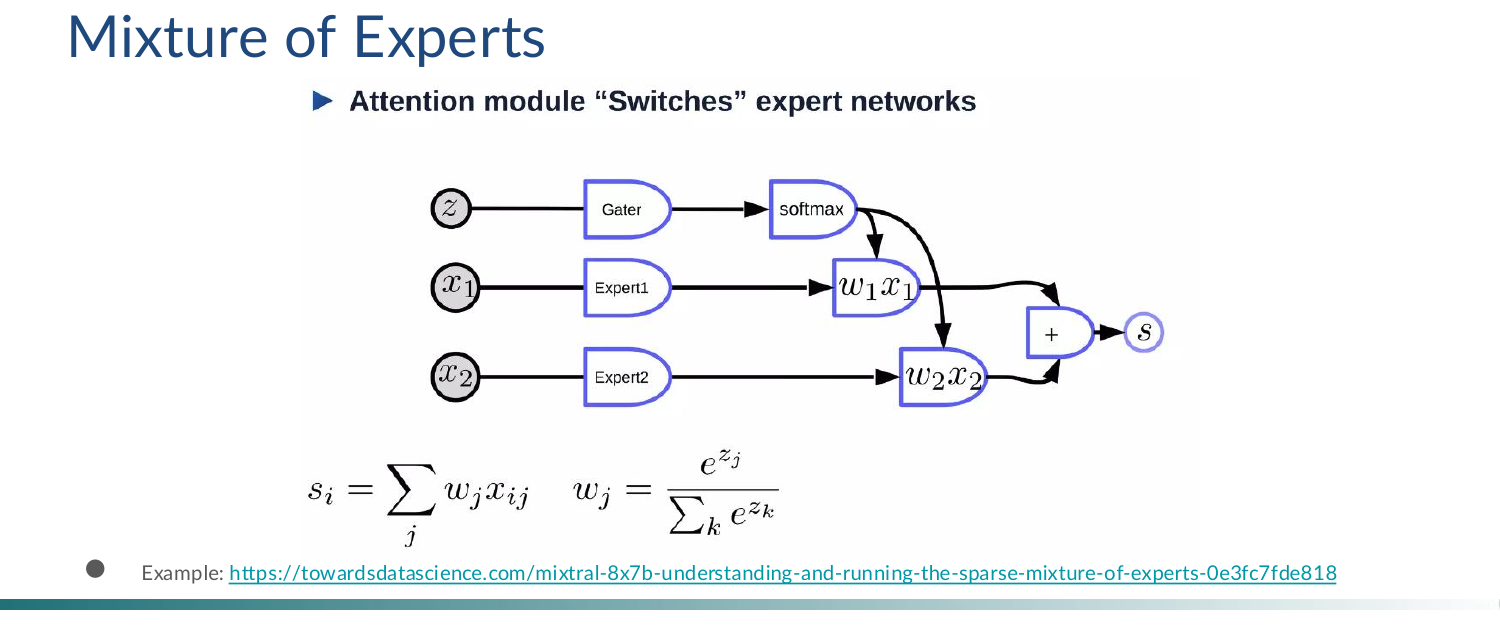
\includegraphics[width=0.82\linewidth]{figures/moe.png}
  \caption{Mixture of Experts: la rete Gater produce i pesi softmax a partire
           da $z$; Expert1 e Expert2 elaborano $x_1$ e $x_2$; le loro uscite
           pesate vengono sommate per produrre $s$.}
  \label{fig:moe}
\end{figure}

Nelle architetture moderne come \textbf{Mixtral 8$\times$7B}
\citep{mixtral2023}, il gating è \textit{sparse}: per ogni token vengono
attivati solo $k$ esperti su $n$ (tipicamente $k{=}2$ su $n{=}8$), con
\textit{top-k routing}. Questo garantisce alta capacità parametrica a basso
costo computazionale, ma introduce la sfida del \textit{load balancing}.

%------------------------------------------------------------
\section{Trasformazioni dei Parametri}
\label{sec:param-transform}

Dato il vettore di parametri interno $\vect{u}$, i pesi operativi $\vect{w}$
sono ottenuti tramite una funzione differenziabile $H$:
\begin{equation}
  \vect{w} = H(\vect{u}).
\end{equation}
Applicando la regola della catena con learning rate $\eta$:
\begin{align}
  u &\leftarrow u - \eta\, \pd{H^T}{u}\, \pd{C^T}{w} \\
  w &\leftarrow w - \eta\, \pd{H}{u}\, \pd{H^T}{u}\, \pd{C^T}{w}
\end{align}
con Jacobiane di dimensioni $[N_u \times N_w]$, $[N_w \times N_u]$,
$[N_w \times 1]$.

\begin{figure}[H]
  \centering
  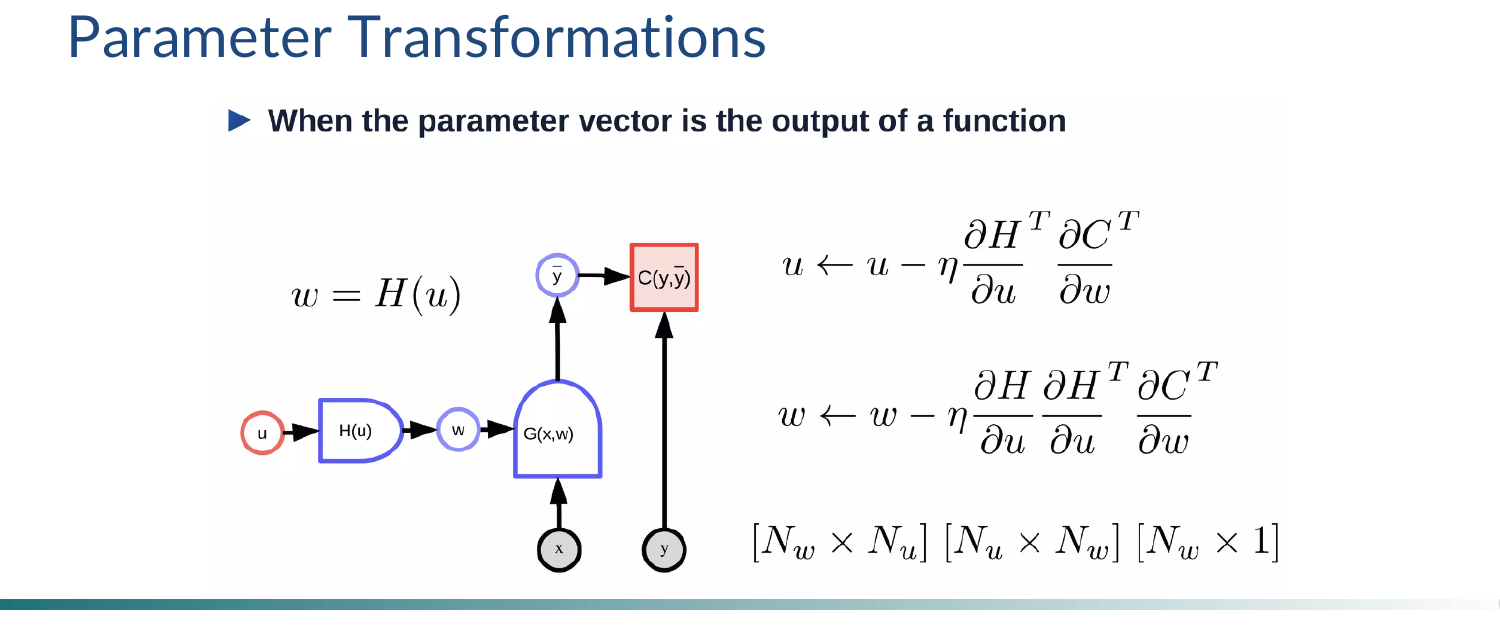
\includegraphics[width=0.82\linewidth]{figures/param_transform.png}
  \caption{Schema della trasformazione parametrica: $u$ passa per $H(u)$
           per produrre $w$, che viene usato in $G(x,w)$. Il backward
           richiede la Jacobiana di $H$ sia rispetto a $u$ sia rispetto a $w$.}
  \label{fig:param_transform}
\end{figure}

\subsection{Weight sharing -- condivisione dei pesi}

Il caso più importante è il \textbf{weight sharing}: $H(\vect{u})$ replica
alcune componenti di $\vect{u}$ in più componenti di $\vect{w}$, ad esempio
$w_1 = w_2 = u_1$, $w_3 = w_4 = u_2$. In backpropagation i gradienti di
tutte le copie vengono \textbf{sommati}:
\begin{equation}
  \pd{C}{u_k} = \sum_{j=1}^{m} \pd{C}{w_{i_j}}.
\end{equation}

\begin{figure}[H]
  \centering
  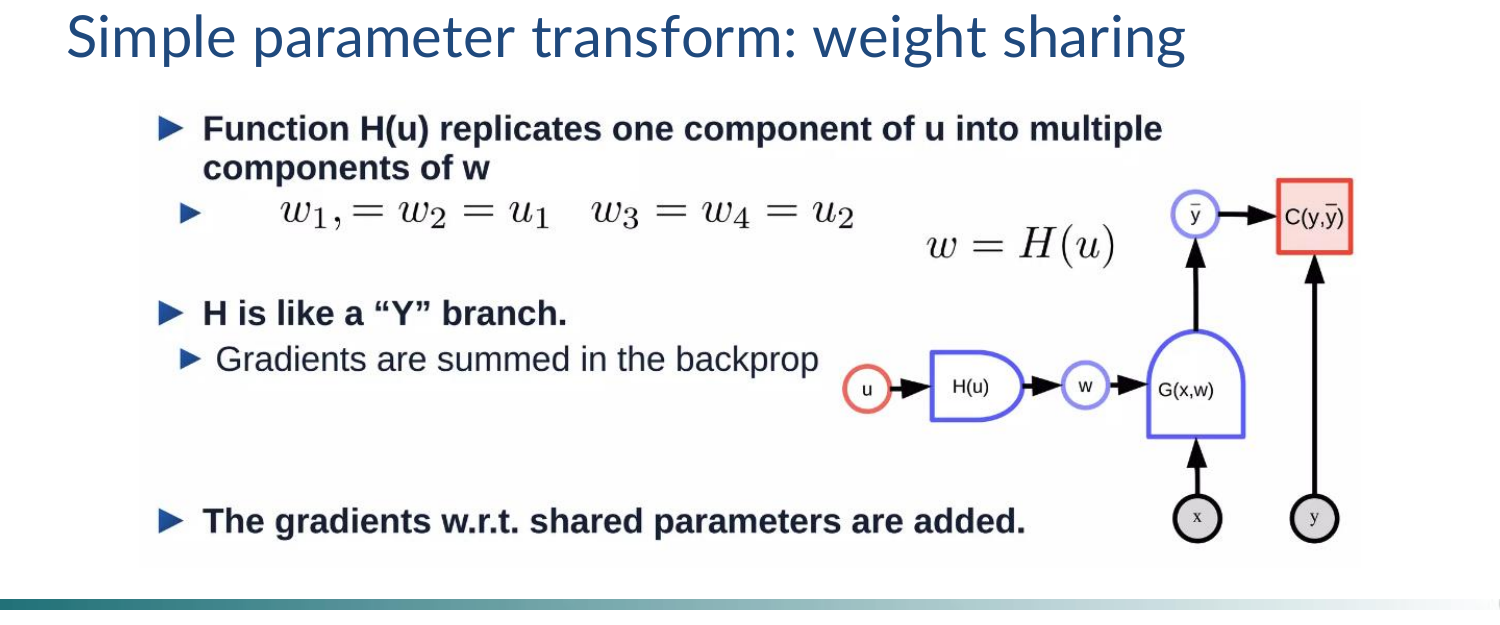
\includegraphics[width=0.82\linewidth]{figures/weight_sharing.png}
  \caption{Weight sharing: $H(u)$ si comporta come un ``ramo Y'', replicando
           il parametro $u_1$ nei pesi $w_1=w_2$ e $u_2$ nei pesi $w_3=w_4$.
           I gradienti w.r.t.\ i parametri condivisi vengono sommati.}
  \label{fig:weight_sharing}
\end{figure}

\subsection{Shared weights per la rilevazione di motif}

Applicando lo stesso $\vect{w}$ a finestre diverse dell'input e raccogliendo
con MAX pooling, si ottiene un rilevatore di motif invariante per traslazione.
Questo schema è esattamente una \textit{convoluzione 1D} seguita da global
max-pooling \citep{lecun1998}.

\begin{figure}[H]
  \centering
  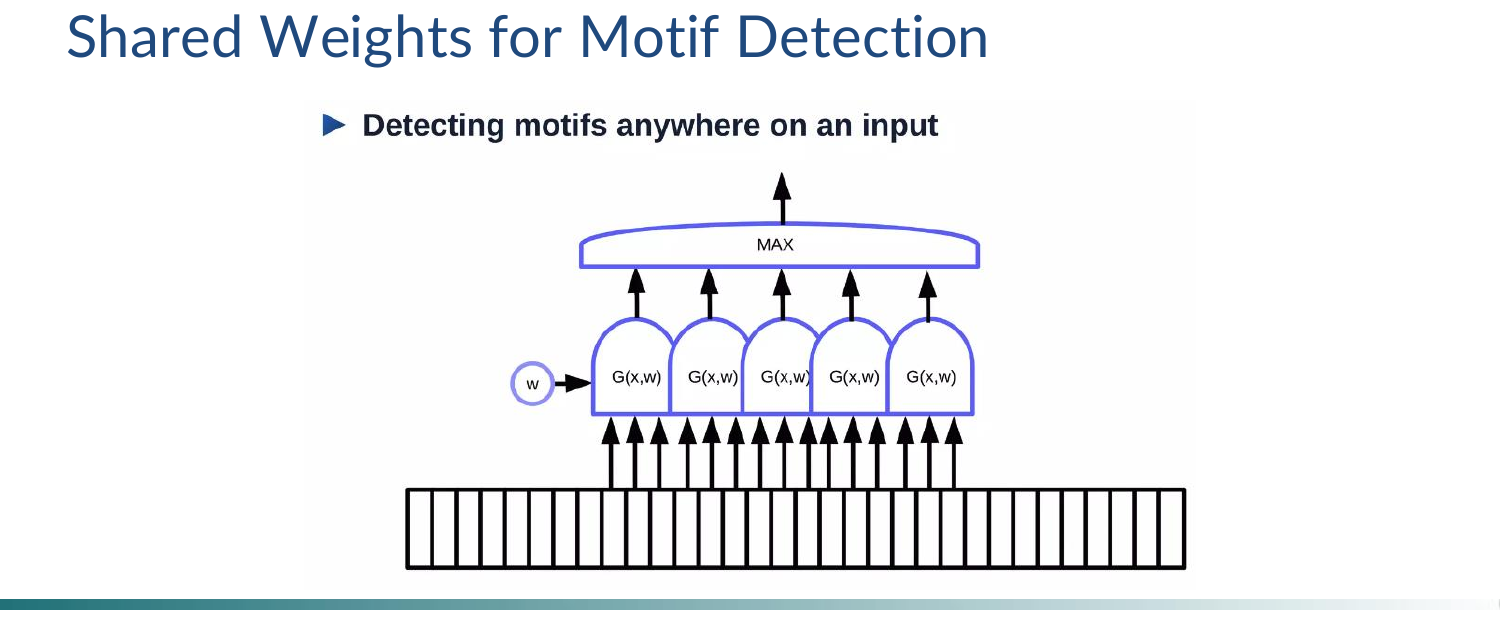
\includegraphics[width=0.82\linewidth]{figures/motif.png}
  \caption{Rilevazione di motif con shared weights: i moduli $G(\vect{x},\vect{w})$
           identici (stesso filtro $w$) scansionano l'input; il MAX pooling
           finale segnala la presenza del motif indipendentemente dalla
           posizione.}
  \label{fig:motif}
\end{figure}

Le CNN \citep{lecun1998} estendono questa idea a 2D, con $K$ filtri in parallelo
e più layer per gerarchie di feature. LeCun e Canziani \citep{lecun2021}
sottolineano come il weight sharing riduca drasticamente i parametri,
costituendo il principale \textit{inductive bias} delle CNN.

%------------------------------------------------------------
\section{Riepilogo}
\label{sec:summary-ch1}

\begin{center}
\begin{tabular}{lll}
  \toprule
  \textbf{Modulo} & \textbf{Formula chiave} & \textbf{Applicazione} \\
  \midrule
  Unità Sigma-Pi     & $s_i=\sum_{jk}u_{ijk}z_kx_j$  & Interaz.\ ordine 2 \\
  Attention module   & $w_j=\softmax(\vect{z})_j$     & Selezione dinamica \\
  Mixture of Experts & attention su reti esperto      & Routing per token \\
  Param.\ Transform  & $\vect{w}=H(\vect{u})$         & Vincoli strutturali \\
  Weight Sharing     & $w_i=w_j=u_k$                  & CNN, RNN \\
  Motif Detection    & $G(\vect{x},\vect{w})$+MAX     & Invarianza trasl. \\
  \bottomrule
\end{tabular}
\end{center}

I moduli moltiplicativi introducono interazioni di secondo ordine tra ingresso
e contesto. Il meccanismo di attenzione ne è il caso differenziabile per
eccellenza, e costituisce il mattone fondamentale dei Transformer
\citep{vaswani2017}. La condivisione dei pesi è la chiave per apprendere da
dataset anche limitati.

%============================================================
%  Capitolo 2 – Learning Representations
%============================================================
\chapter{Learning Representations}
\label{ch:learning-repr}

Questo capitolo affronta una domanda fondamentale: \textit{perché le reti profonde
funzionano meglio di quelle shallow?} La risposta passa per il concetto di
\textbf{rappresentazione}: trasformare i dati grezzi in uno spazio in cui il
problema diventi più facile da risolvere \citep{bishop2024, lecun2021}.

%------------------------------------------------------------
\section{Limiti dei Classificatori Lineari}
\label{sec:linear-limits}

Un \textbf{classificatore lineare} assegna la classe in base al segno di una
combinazione lineare delle feature:
\begin{equation}
  \bar{y} = \operatorname{sign}\!\left(\sum_{i=1}^{N} w_i x_i + b\right).
\end{equation}
Geometricamente, il classificatore partiziona lo spazio in due semispazi
separati dall'iperpiano $\sum_i w_i x_i + b = 0$. Il vettore $\vect{w}$
è la normale all'iperpiano e ne determina l'orientamento; $-b/w_1$ ne fissa
l'intercetta.

\begin{figure}[H]
  \centering
  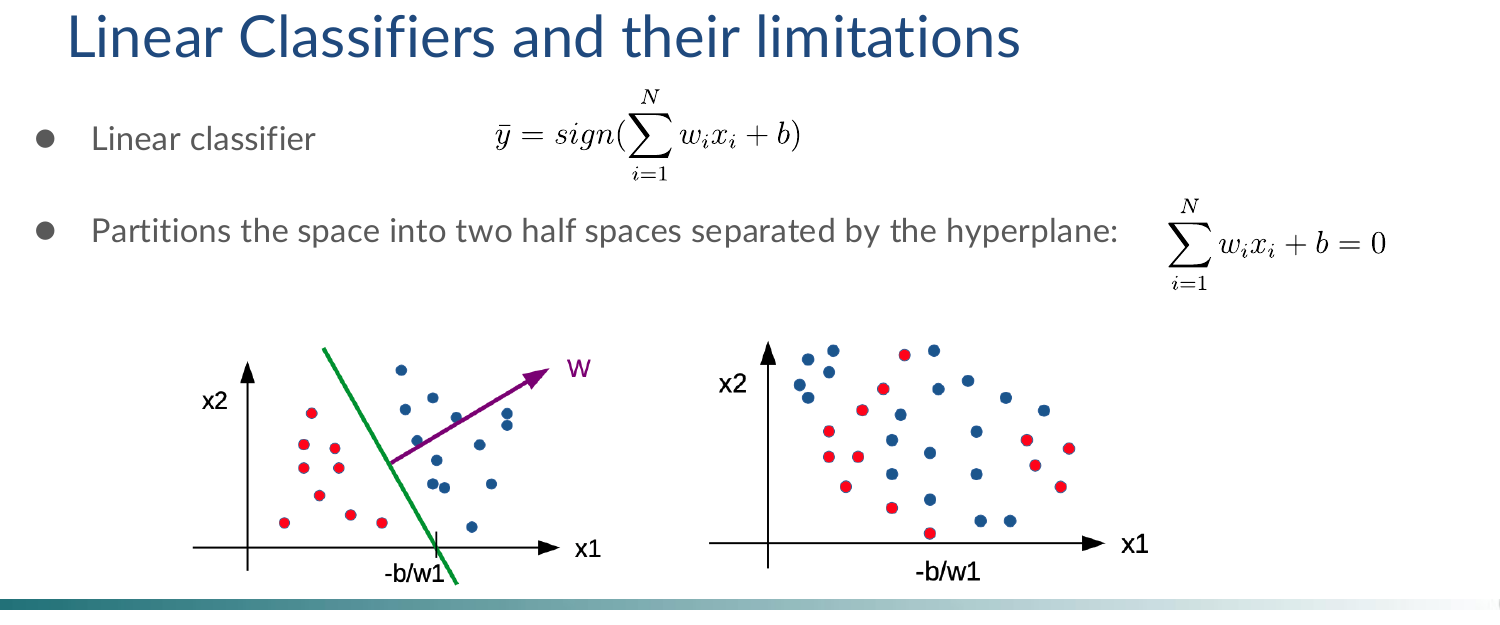
\includegraphics[width=0.88\linewidth]{figures/lr02_linear_classifier.png}
  \caption{Classificatore lineare in 2D. Sinistra: caso separabile linearmente
           -- l'iperpiano (retta verde) divide correttamente le due classi.
           Destra: caso non separabile linearmente -- nessuna retta può separare
           i punti rossi da quelli blu.}
  \label{fig:linear_classifier}
\end{figure}

Il limite fondamentale dei classificatori lineari è formalizzato dal
\textbf{Teorema di Cover (1966)}: la probabilità che una dicotomia casuale
di $P$ punti in $N$ dimensioni sia linearmente separabile tende a zero
quando $P \gg N$.

\begin{figure}[H]
  \centering
  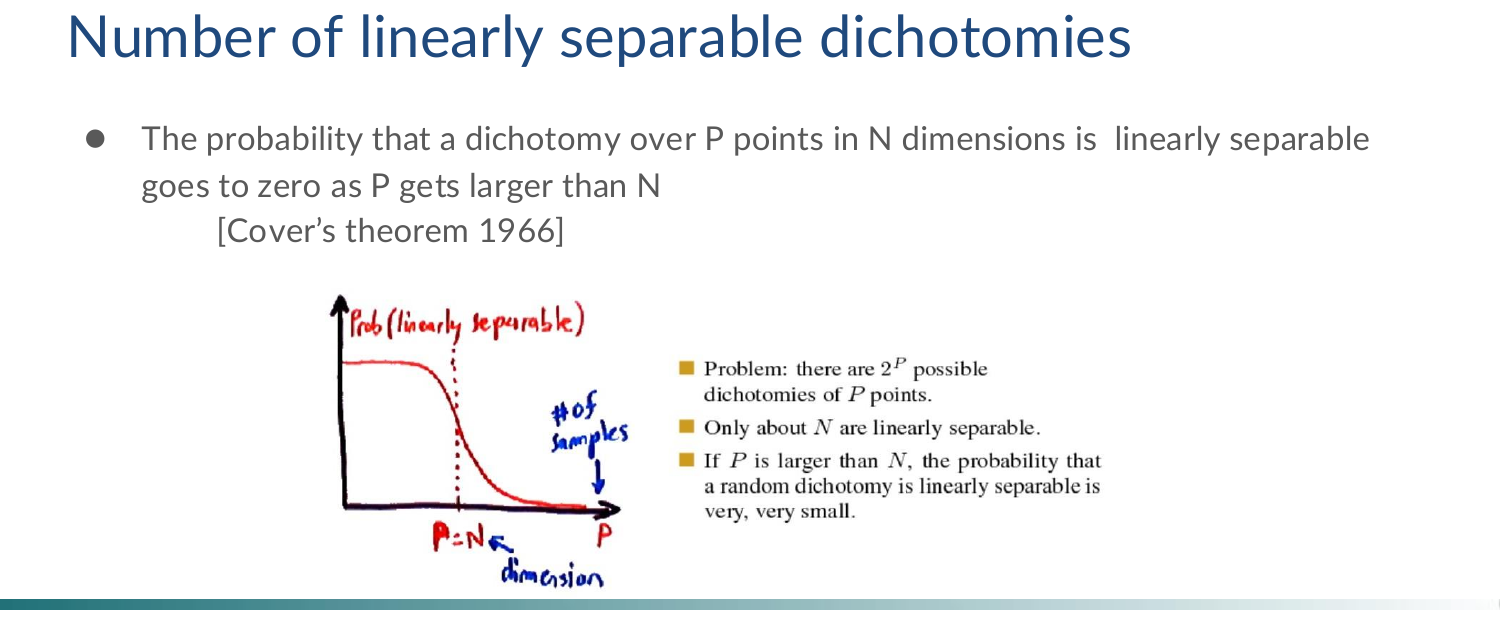
\includegraphics[width=0.75\linewidth]{figures/lr02_cover_theorem.png}
  \caption{Teorema di Cover: la probabilità di separabilità lineare crolla
           bruscamente non appena il numero di campioni $P$ supera la
           dimensionalità $N$. Esistono $2^P$ possibili dicotomie, ma solo
           circa $N$ sono linearmente separabili.}
  \label{fig:cover_theorem}
\end{figure}

In pratica: con $P \gg N$, quasi nessuna dicotomia casuale è linearmente
separabile. Per classificare dati reali complessi, occorre una
\textbf{trasformazione non lineare} che renda il problema separabile.

%------------------------------------------------------------
\section{La Soluzione: Rappresentazioni (Feature)}
\label{sec:solution-repr}

La soluzione è costruire un \textbf{estrattore di feature} che trasformi
l'input grezzo in una rappresentazione in cui un classificatore lineare
possa operare efficacemente. L'estrattore deve essere \emph{non lineare}:
una trasformazione lineare non cambia la separabilità del problema.

\begin{figure}[H]
  \centering
  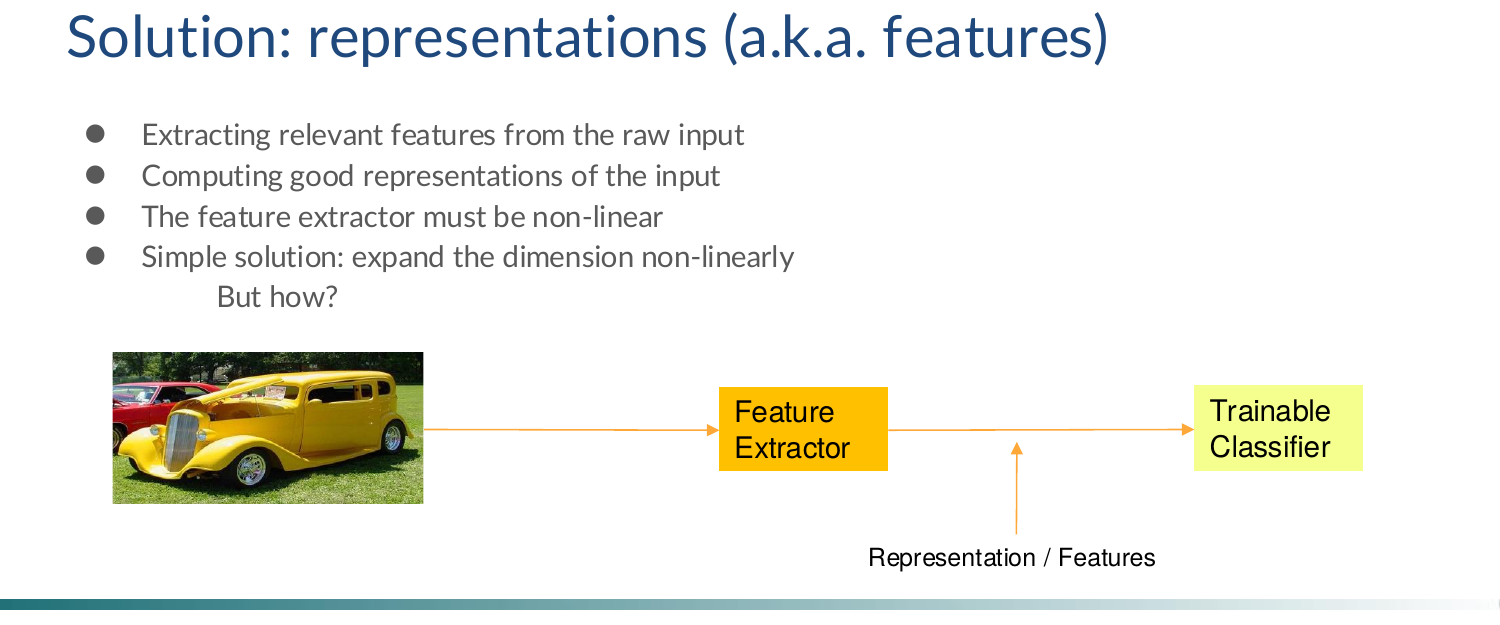
\includegraphics[width=0.80\linewidth]{figures/lr02_solution_repr.png}
  \caption{Soluzione con rappresentazioni: il blocco Feature Extractor
           trasforma l'input grezzo in una rappresentazione/feature; su queste
           opera un classificatore trainable. Nel DL anche l'estrattore è
           addestrato end-to-end.}
  \label{fig:solution_repr}
\end{figure}

Il principio di base è \textbf{espandere la dimensionalità} in modo non
lineare: in uno spazio di dimensione maggiore, punti che erano non separabili
diventano separabili con alta probabilità (per il Teorema di Cover, la
probabilità di separabilità cresce con $N$).

\subsection{Idee per l'estrazione generica di feature}

Esistono diverse strategie ``generiche'' per costruire feature non lineari
\reflecun{W2}:

\begin{itemize}
  \item \textbf{Space tiling}: si suddivide lo spazio di input in regioni e
        si usano indicatori di appartenenza come feature.
  \item \textbf{Random projections}: si proietta l'input su vettori casuali
        seguiti da non-linearità (es.\ ReLU). Alla base dei \textit{reservoir
        computing} e delle \textit{random features} per kernel approximation.
  \item \textbf{Feature monomiali} (cross-products): il feature extractor
        calcola prodotti di coppie (o triple, ecc.) di variabili di input;
        un classificatore lineare su queste feature calcola un polinomio
        dell'input.
  \item \textbf{Radial Basis Functions (RBF)}: feature del tipo
        $\phi_k(x) = \exp(-\|x - c_k\|^2 / 2\sigma^2)$, con centri $c_k$
        fissati o appresi.
  \item \textbf{Kernel machines}: generalizzano le RBF attraverso funzioni
        kernel $K(x^j, x)$; le SVM ne sono l'esempio principale.
\end{itemize}

\subsection{Feature monomiali e limiti}

\begin{figure}[H]
  \centering
  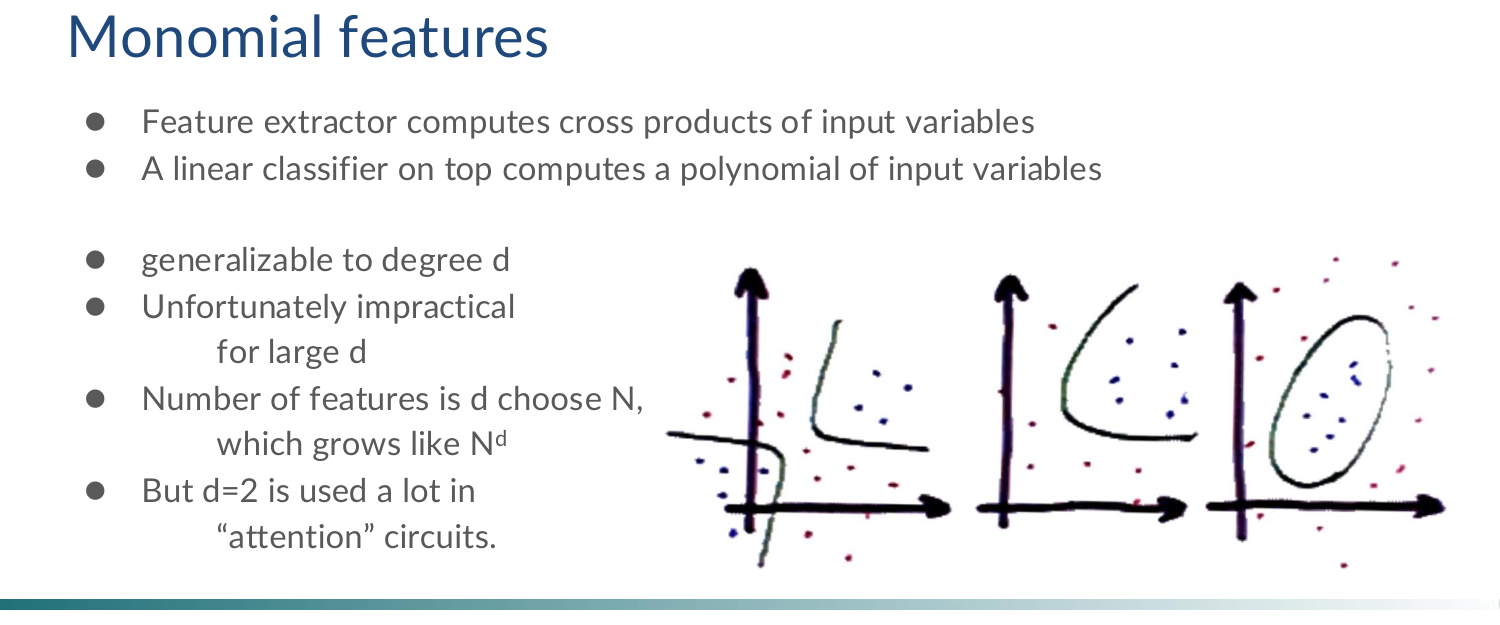
\includegraphics[width=0.82\linewidth]{figures/lr02_monomial.png}
  \caption{Feature monomiali: aggiungendo il termine quadratico $x_1 x_2$
           (o più in generale prodotti di grado $d$) come feature, un
           classificatore lineare può separare pattern che erano non lineari
           nell'input originale -- ad esempio boundary ellittici o a forma
           di C.}
  \label{fig:monomial}
\end{figure}

Le feature monomiali di grado $d$ su $N$ variabili producono
$\binom{N+d}{d} \sim N^d$ feature: questo numero cresce esponenzialmente con
$d$, rendendo il metodo impraticabile per grandi $d$.
Tuttavia, il caso $d=2$ è molto usato nei circuiti di
\textit{attention} (si veda il Cap.\,\ref{ch:basic-arch}), in quanto corrisponde
esattamente alle unità Sigma-Pi.

%------------------------------------------------------------
\section{Reti Shallow vs Reti Profonde}
\label{sec:shallow-vs-deep}

\subsection{Le reti shallow sono approssimatori universali}

Un risultato teorico fondamentale afferma che una rete neurale a 2 layer con
numero sufficiente di unità nascoste può approssimare qualsiasi funzione
continua con precisione arbitraria \refbishop{6}. Lo stesso vale per le
\textbf{Support Vector Machine} con kernel:
\begin{equation}
  G(X,\alpha) = \sum_j \alpha_j K(X^j, X),
\end{equation}
dove il primo layer calcola i kernel $K(X^j, X)$ usando i campioni di
training come template, e il secondo layer è una combinazione lineare con
pesi $\alpha_j$.

\begin{figure}[H]
  \centering
  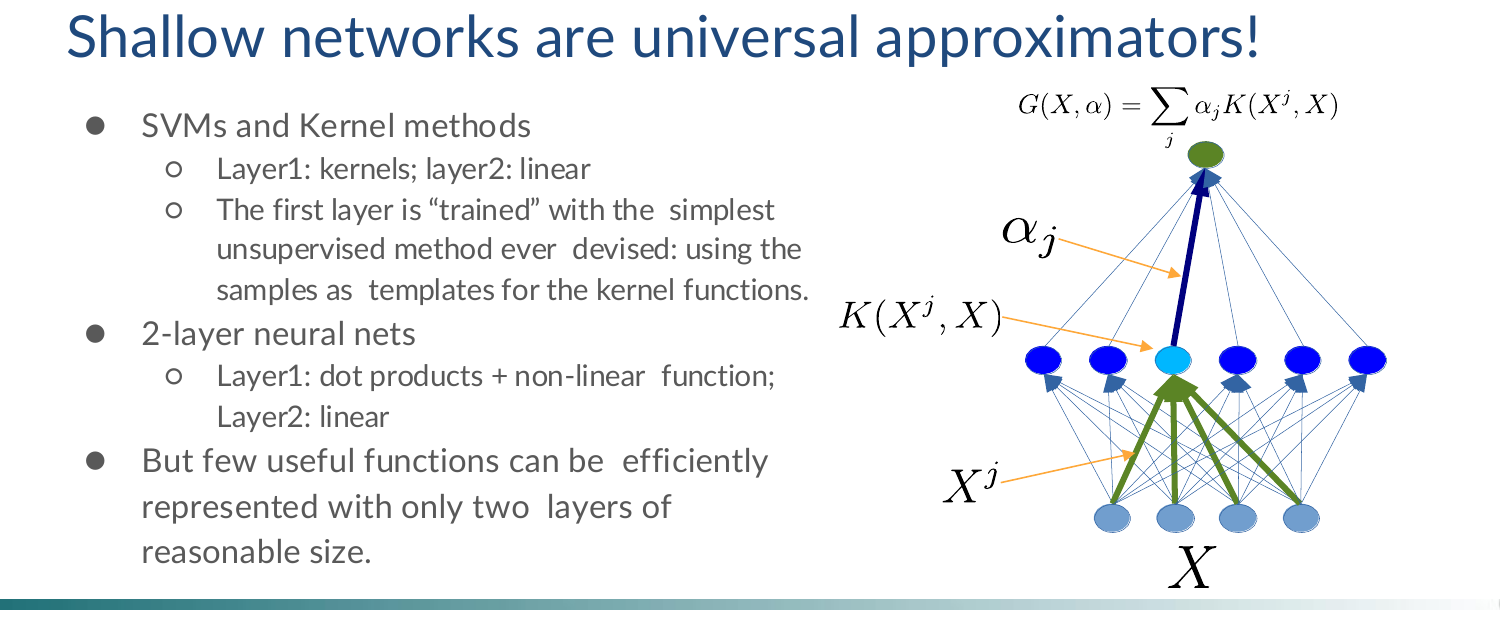
\includegraphics[width=0.80\linewidth]{figures/lr02_shallow_universal.png}
  \caption{Architettura di una kernel machine (SVM): il primo layer calcola
           $K(X^j, X)$ per ogni campione di training $X^j$; il secondo layer
           combina linearmente le attivazioni con pesi $\alpha_j$.}
  \label{fig:shallow_universal}
\end{figure}

\subsection{Perché servono architetture profonde?}

Se le reti shallow sono universali, perché usare reti profonde? Il
\textbf{dilemma del teorico} pone esattamente questa domanda.

\begin{figure}[H]
  \centering
  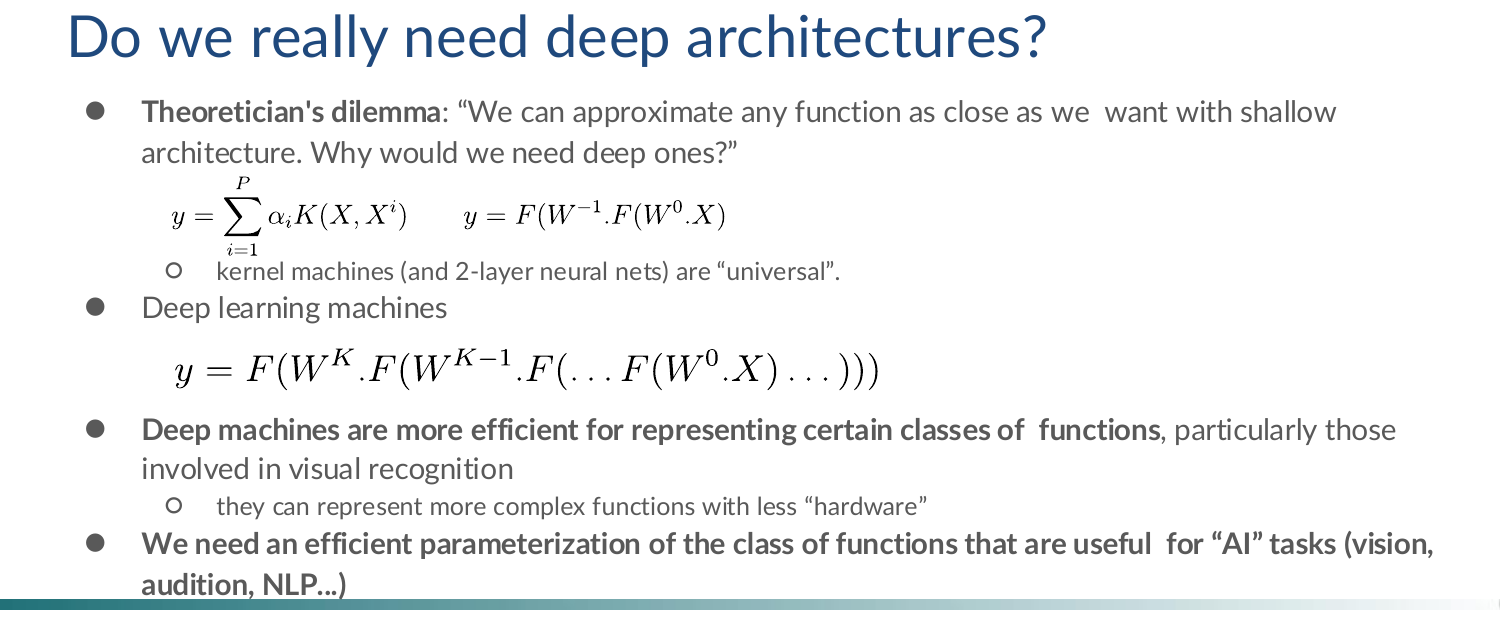
\includegraphics[width=0.88\linewidth]{figures/lr02_deep_vs_shallow.png}
  \caption{Confronto tra reti shallow e profonde: una rete shallow (kernel
           machine o 2-layer net) può rappresentare qualunque funzione, ma
           richiede un numero esponenziale di unità per funzioni complesse;
           una rete profonda $y = F(W^K \cdot F(\ldots F(W^0 \cdot X)\ldots))$
           le rappresenta in modo molto più efficiente.}
  \label{fig:deep_vs_shallow}
\end{figure}

La risposta è nell'\textbf{efficienza della rappresentazione}: le reti
profonde possono rappresentare certe classi di funzioni -- in particolare
quelle coinvolte nel riconoscimento visivo -- con molti meno parametri
rispetto alle reti shallow \citep{bishop2024}. Come argomenta
\citet{lecun2021}, una rete profonda \textit{scambia spazio con tempo}
(o ampiezza con profondità): più layer sequenziali ma meno hardware parallelo.

%------------------------------------------------------------
\section{Invariant Feature Learning}
\label{sec:invariant-features}

L'idea di base per imparare feature invarianti è la seguente
\reflecun{W2}:

\begin{enumerate}
  \item \textbf{Espandere} l'input non linearmente in uno spazio ad alta
        dimensionalità (feature instabili ma discriminative).
  \item \textbf{Aggregare} regioni del nuovo spazio (pooling, proiezione,
        riduzione di dimensionalità) per ottenere feature stabili e invarianti.
\end{enumerate}

\begin{figure}[H]
  \centering
  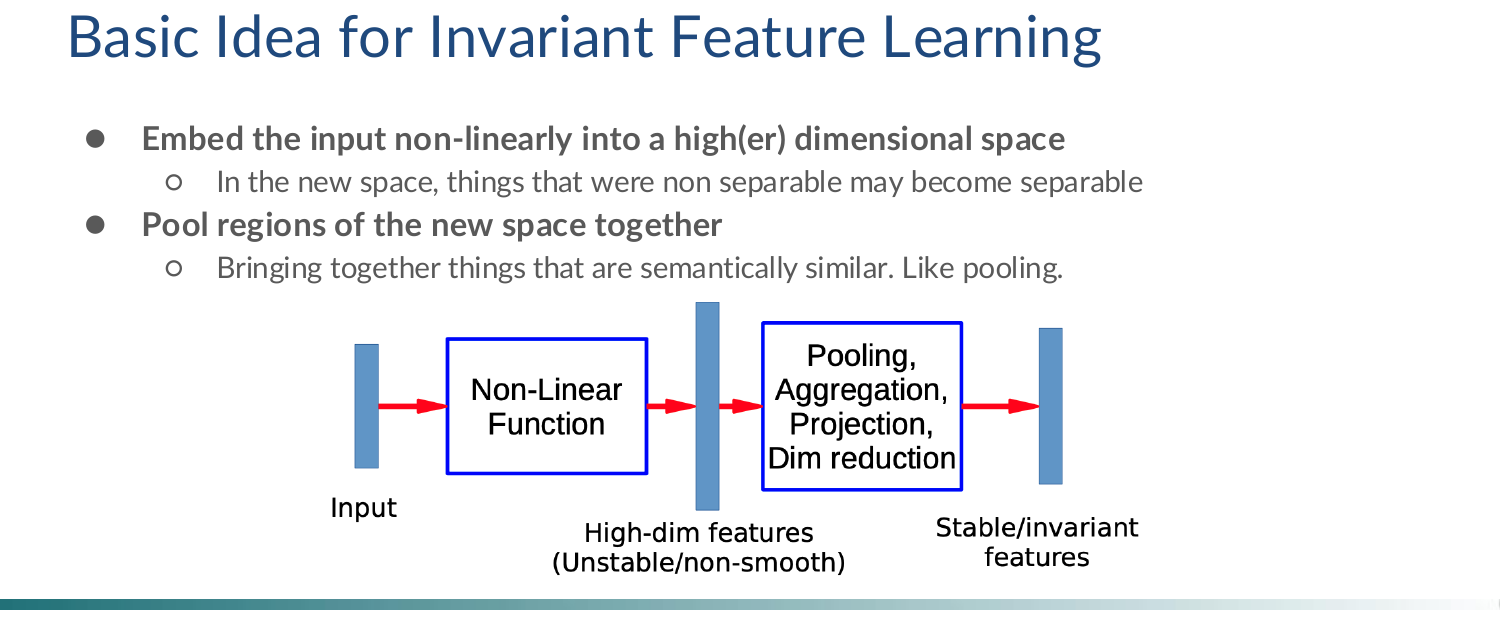
\includegraphics[width=0.82\linewidth]{figures/lr02_invariant_learning.png}
  \caption{Schema dell'invariant feature learning: la funzione non lineare
           espande l'input in feature ad alta dimensione (instabili), che
           vengono poi aggregate tramite pooling/aggregazione/dim.\
           reduction per produrre feature stabili e invarianti.}
  \label{fig:invariant_learning}
\end{figure}

%------------------------------------------------------------
\section{L'Ipotesi del Manifold}
\label{sec:manifold}

\begin{definizione}[Manifold Hypothesis]
I dati naturali vivono in un \textbf{manifold non lineare a bassa dimensione}
immerso nello spazio ad alta dimensione. Le variabili nei dati naturali sono
mutuamente dipendenti, per cui la variabilità intrinseca è molto più bassa
della dimensione nominale.
\end{definizione}

\begin{figure}[H]
  \centering
  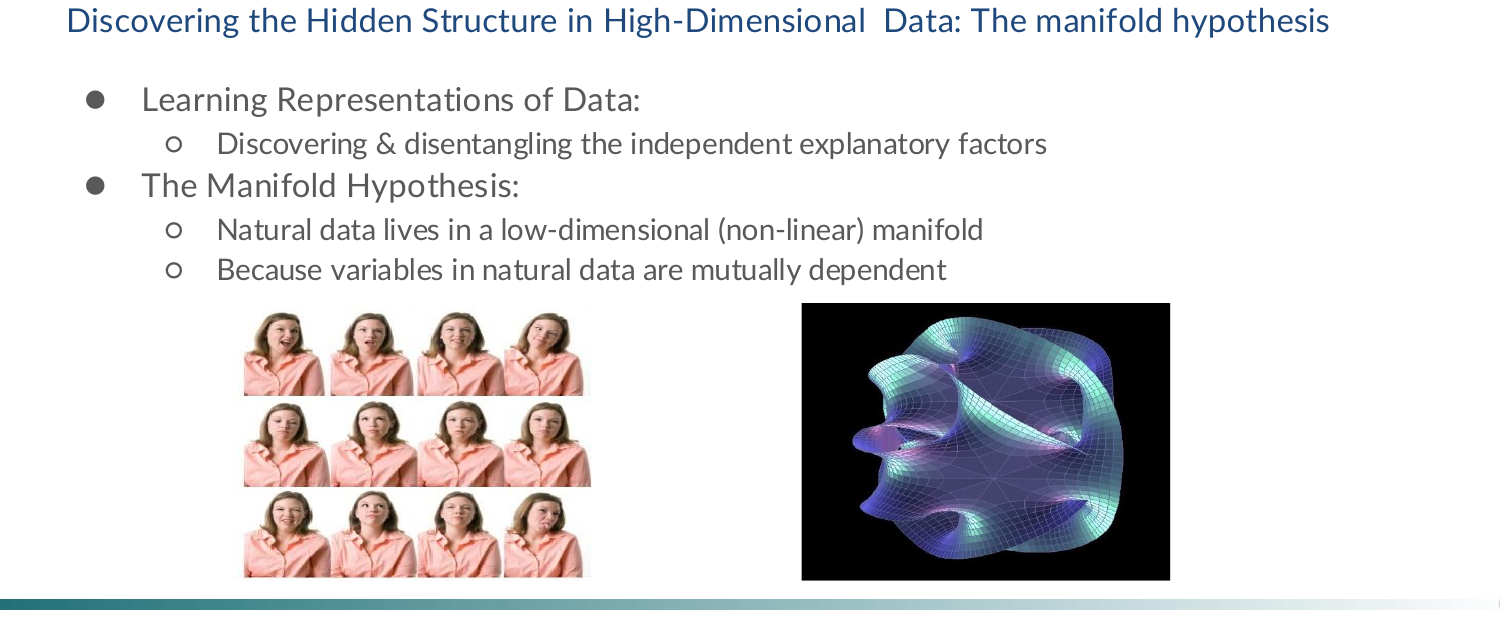
\includegraphics[width=0.88\linewidth]{figures/lr02_manifold_hypothesis.png}
  \caption{L'ipotesi del manifold: le immagini di volti (sinistra) variano
           in espressione, posa, illuminazione -- ma questa variabilità
           appartiene a un manifold a bassa dimensione (destra), non a tutto
           lo spazio dei pixel.}
  \label{fig:manifold_hypothesis}
\end{figure}

\paragraph{Esempio: immagini di volti.}
Un'immagine $1000 \times 1000$ pixel ha $10^6$ dimensioni. Tuttavia un volto
è descritto da soli 3 coordinate cartesiane, 3 angoli di Eulero e meno di 50
muscoli facciali: il manifold delle immagini di un volto ha quindi meno di 56
dimensioni effettive.

\begin{figure}[H]
  \centering
  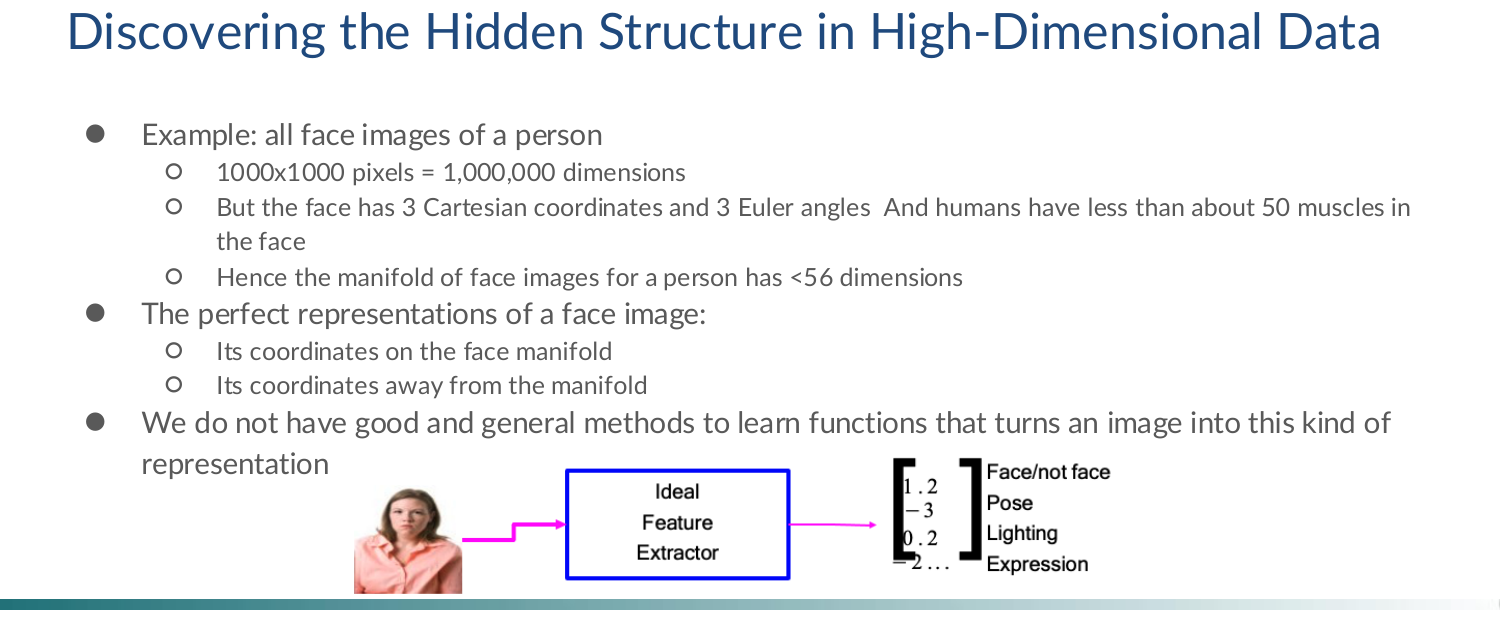
\includegraphics[width=0.82\linewidth]{figures/lr02_face_manifold.png}
  \caption{La rappresentazione ideale di un'immagine facciale ne estrae le
           coordinate sul manifold (pose, lighting, expression\ldots) come
           vettore compatto. Non disponiamo ancora di metodi generali per
           imparare questa funzione.}
  \label{fig:face_manifold}
\end{figure}

%------------------------------------------------------------
\section{Disentangling e Apprendimento delle Rappresentazioni}
\label{sec:disentangling}

L'obiettivo del \textbf{representation learning} è scoprire e
\emph{disintrecciare} (disentangle) i fattori di variazione indipendenti
che generano i dati.

\begin{figure}[H]
  \centering
  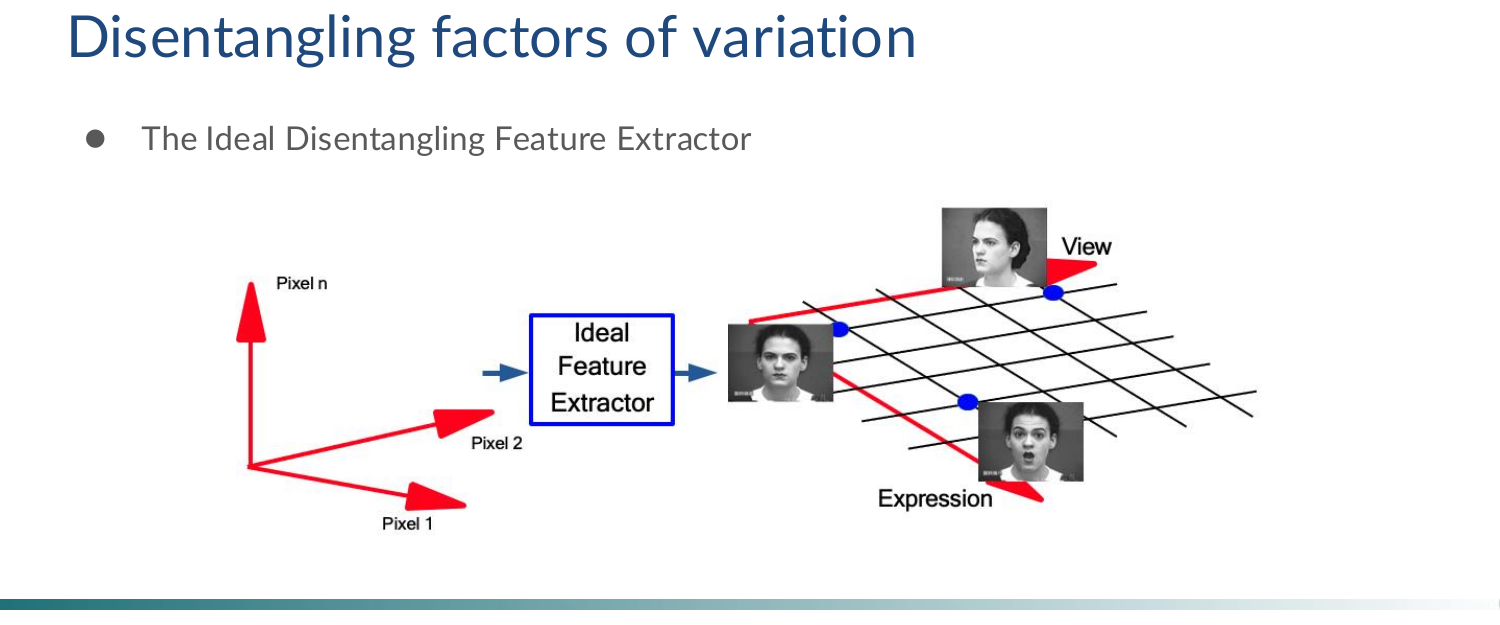
\includegraphics[width=0.88\linewidth]{figures/lr02_disentangling.png}
  \caption{L'ideal feature extractor mappa lo spazio dei pixel (sinistra)
           nel manifold dei volti (destra), dove le coordinate corrispondono
           a fattori interpretabili come ``view'' (punto di vista) e
           ``expression'' (espressione). Ogni punto blu nel manifold
           corrisponde a un'immagine specifica.}
  \label{fig:disentangling}
\end{figure}

Un esempio concreto di manifold appreso è mostrato nel lavoro di
Hadsell et al.\ (CVPR 2006): immagini di aeroplani in diverse rotazioni
sono disposte su una curva chiusa nell'embedding space, rispecchiando
la struttura continua della rotazione.

\begin{figure}[H]
  \centering
  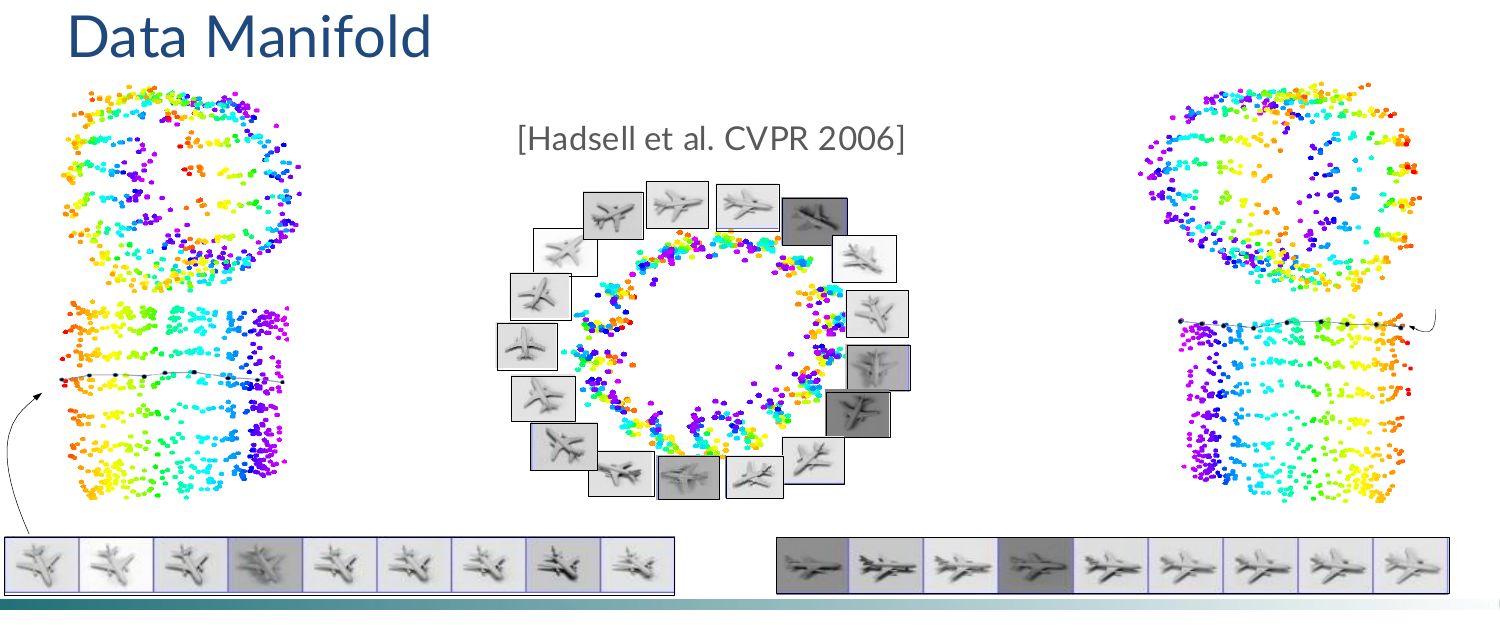
\includegraphics[width=0.88\linewidth]{figures/lr02_data_manifold.png}
  \caption{Data manifold appreso [Hadsell et al., CVPR 2006]: le immagini
           di aeroplani in diverse orientazioni formano una struttura ciclica
           coerente nello spazio di embedding -- punti vicini corrispondono a
           immagini visivamente simili.}
  \label{fig:data_manifold}
\end{figure}

%------------------------------------------------------------
\section{Architetture Multilayer = Struttura Compositiva}
\label{sec:multilayer}

I dati naturali hanno una \textbf{struttura compositiva}: sono costruiti
gerarchicamente da elementi via via più astratti. Le reti neurali multilayer
sfruttano questa struttura, con ogni layer che apprende un livello di
astrazione \citep{lecun2021}.

\begin{figure}[H]
  \centering
  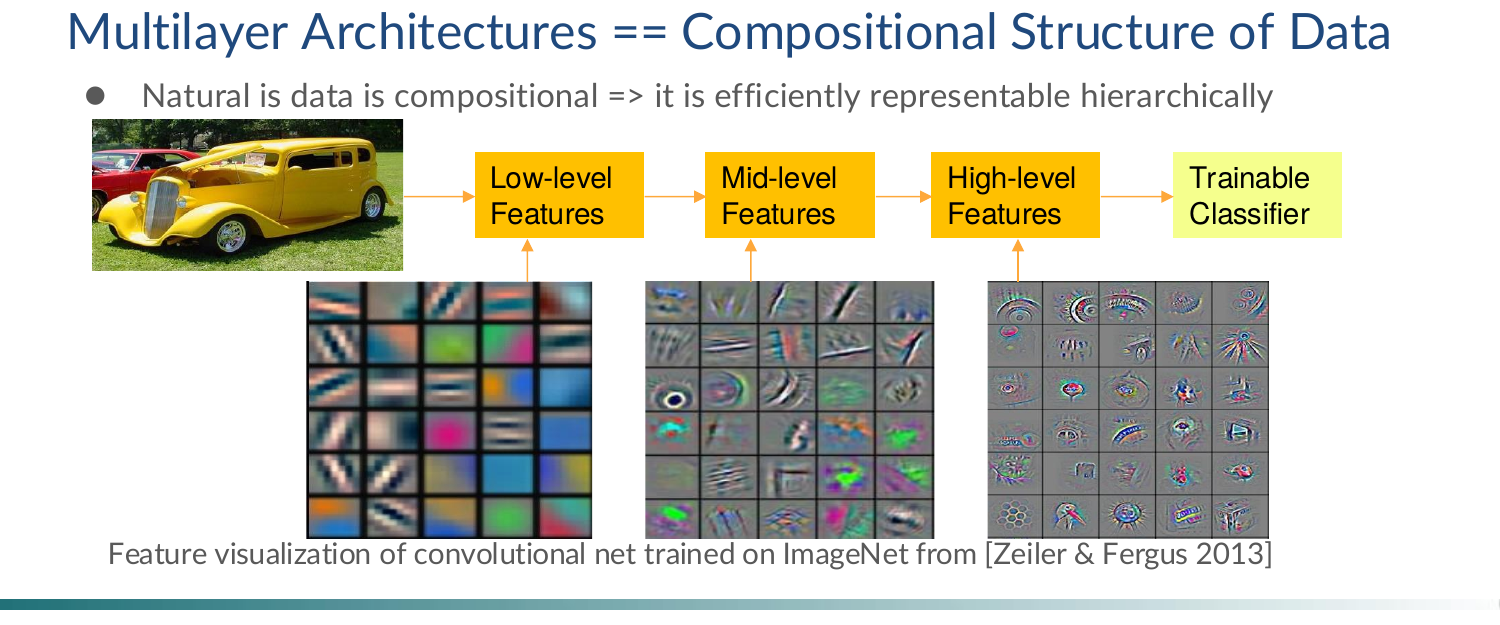
\includegraphics[width=0.92\linewidth]{figures/lr02_compositional.png}
  \caption{Le architetture multilayer corrispondono alla struttura compositiva
           dei dati. La visualizzazione delle feature di una CNN addestrata su
           ImageNet [Zeiler \& Fergus, 2013] mostra: layer bassi = edge e
           texture, layer intermedi = parti di oggetti, layer alti = concetti
           semantici.}
  \label{fig:compositional}
\end{figure}

\paragraph{Gerarchia di rappresentazioni nei diversi domini.}

\begin{figure}[H]
  \centering
  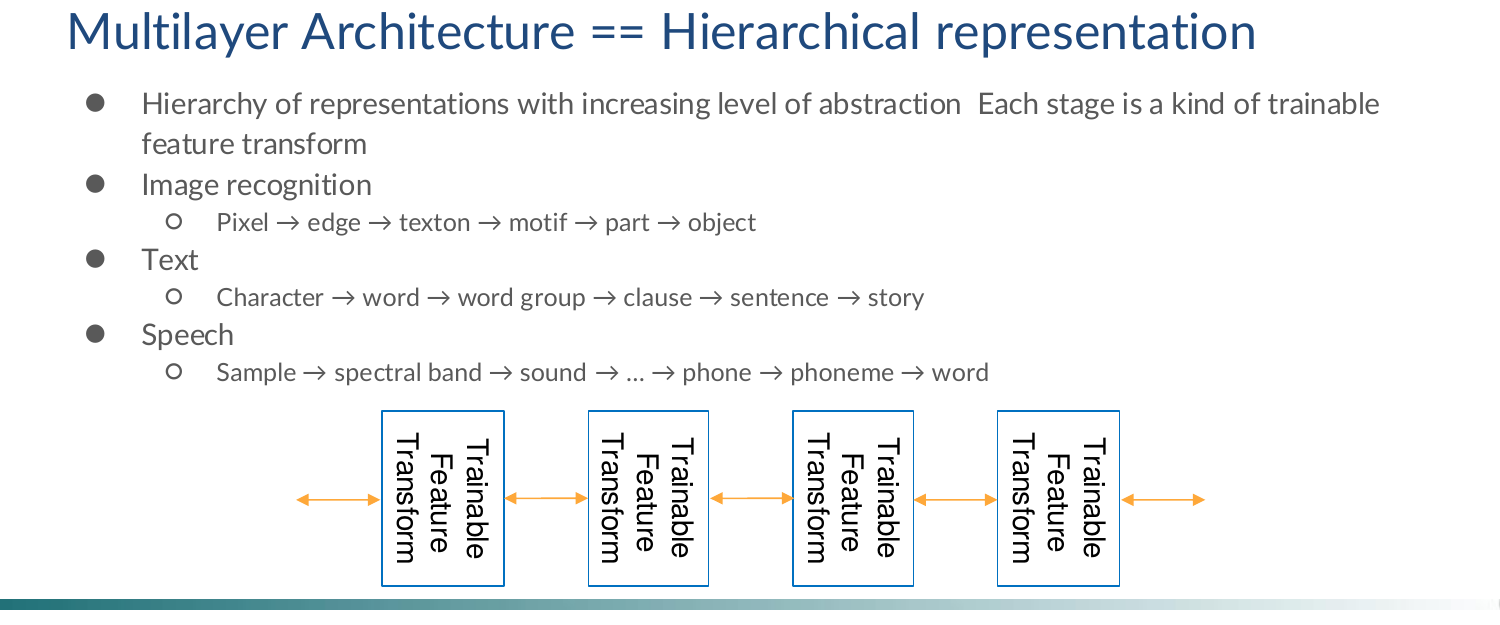
\includegraphics[width=0.82\linewidth]{figures/lr02_hierarchical.png}
  \caption{Architettura multilayer come rappresentazione gerarchica: ogni
           blocco ``Trainable Feature Transform'' corrisponde a un livello di
           astrazione. Le frecce bidirezionali indicano che ogni modulo
           può essere addestrato con backpropagation.}
  \label{fig:hierarchical}
\end{figure}

La gerarchia di astrazioni varia a seconda del dominio:
\begin{itemize}
  \item \textbf{Immagini}: pixel $\to$ edge $\to$ texton $\to$ motif
        $\to$ parte $\to$ oggetto.
  \item \textbf{Testo}: carattere $\to$ parola $\to$ gruppo di parole
        $\to$ proposizione $\to$ frase $\to$ storia.
  \item \textbf{Audio}: campione $\to$ banda spettrale $\to$ suono
        $\to$ \ldots $\to$ fonema $\to$ parola.
\end{itemize}

L'efficienza delle architetture profonde è spiegata da
\citet{lecun2021} e da Bengio \& LeCun (2007): una rete profonda
\textit{scambia ampiezza con profondità} -- più layer sequenziali ma
meno hardware parallelo -- riuscendo a rappresentare funzioni complesse
con molti meno parametri rispetto a una rete shallow.

%------------------------------------------------------------
\section{Riepilogo}
\label{sec:summary-ch2}

\begin{center}
\begin{tabular}{lll}
  \toprule
  \textbf{Concetto} & \textbf{Idea chiave} & \textbf{Implicazione} \\
  \midrule
  Classificatore lineare & $\bar{y}=\operatorname{sign}(\vect{w}^T\vect{x}+b)$ & Limite: non sep. lineare \\
  Teorema di Cover       & Prob.\ sep.\ $\to 0$ se $P \gg N$      & Serve non-linearità \\
  Feature monomiali      & Cross-products di grado $d$             & $O(N^d)$ feature \\
  Reti shallow           & Approssimatori universali               & Ma inefficienti \\
  Reti profonde          & $y = F(W^K \cdot F(\ldots))$           & Più efficienti \\
  Manifold Hypothesis    & Dati su manifold bassa-dim.             & Motiva il DL \\
  Disentangling          & Separare i fattori di variazione        & Obiettivo del repr.\ learning \\
  Struttura compositiva  & Pixel $\to$ edge $\to$ parte $\to$ obj & Giustifica i multilayer \\
  \bottomrule
\end{tabular}
\end{center}

Le reti neurali profonde sono giustificate non solo dall'approssimazione
universale (che vale anche per reti shallow), ma dalla loro
\textbf{efficienza parametrica} nel rappresentare le funzioni utili per i
compiti AI. L'ipotesi del manifold e la struttura compositiva dei dati
naturali forniscono le basi teoriche per questa efficienza.

%============================================================
%  Capitolo 3 – Activation Functions
%============================================================
\chapter{Activation Functions}
\label{ch:activation-functions}

Le \textbf{funzioni di attivazione} sono il cuore della non-linearità nelle reti neurali.
Senza di esse, una rete a più strati si ridurrebbe a una semplice trasformazione lineare,
indipendentemente dalla profondità \citep{bishop2024}.
Come osserva Canziani nelle note NYU-DL, ogni layer di una rete tradizionale alterna
un blocco \emph{lineare} $\mathbf{s}_{k+1} = W_k \mathbf{z}_k$ a un blocco \emph{non lineare}
$\mathbf{z}_k = h(\mathbf{s}_k)$, dove $h$ è appunto la funzione di attivazione.
La scelta di $h$ influenza profondamente la velocità di convergenza, la stabilità
del gradiente e le capacità espressive della rete.

%------------------------------------------------------------
\section{Il Problema del Vanishing Gradient}
\label{sec:vanishing-gradient}

Il principale limite delle funzioni di attivazione \textbf{saturanti} (es.\ Sigmoid,
Tanh) è il cosiddetto \textbf{vanishing gradient problem}.
La retropropagazione moltiplica gradienti attraverso ogni layer: se ogni fattore è
$\ll 1$, il segnale si azzera esponenzialmente procedendo verso i layer iniziali.

Per la Sigmoid, il gradiente massimo è:
\begin{equation}
  \max_x \frac{\partial\,\sigma(x)}{\partial x}
  = \frac{1}{4} = 0{,}25 \qquad \text{(raggiunto in } x=0\text{)},
\end{equation}
e si avvicina a zero sia per $x \to +\infty$ sia per $x \to -\infty$.
In una rete con $L$ layer, il gradiente che torna al primo layer scala come
$(0{,}25)^L$: già per $L=10$ si ottiene $\approx 10^{-6}$.

\begin{figure}[H]
  \centering
  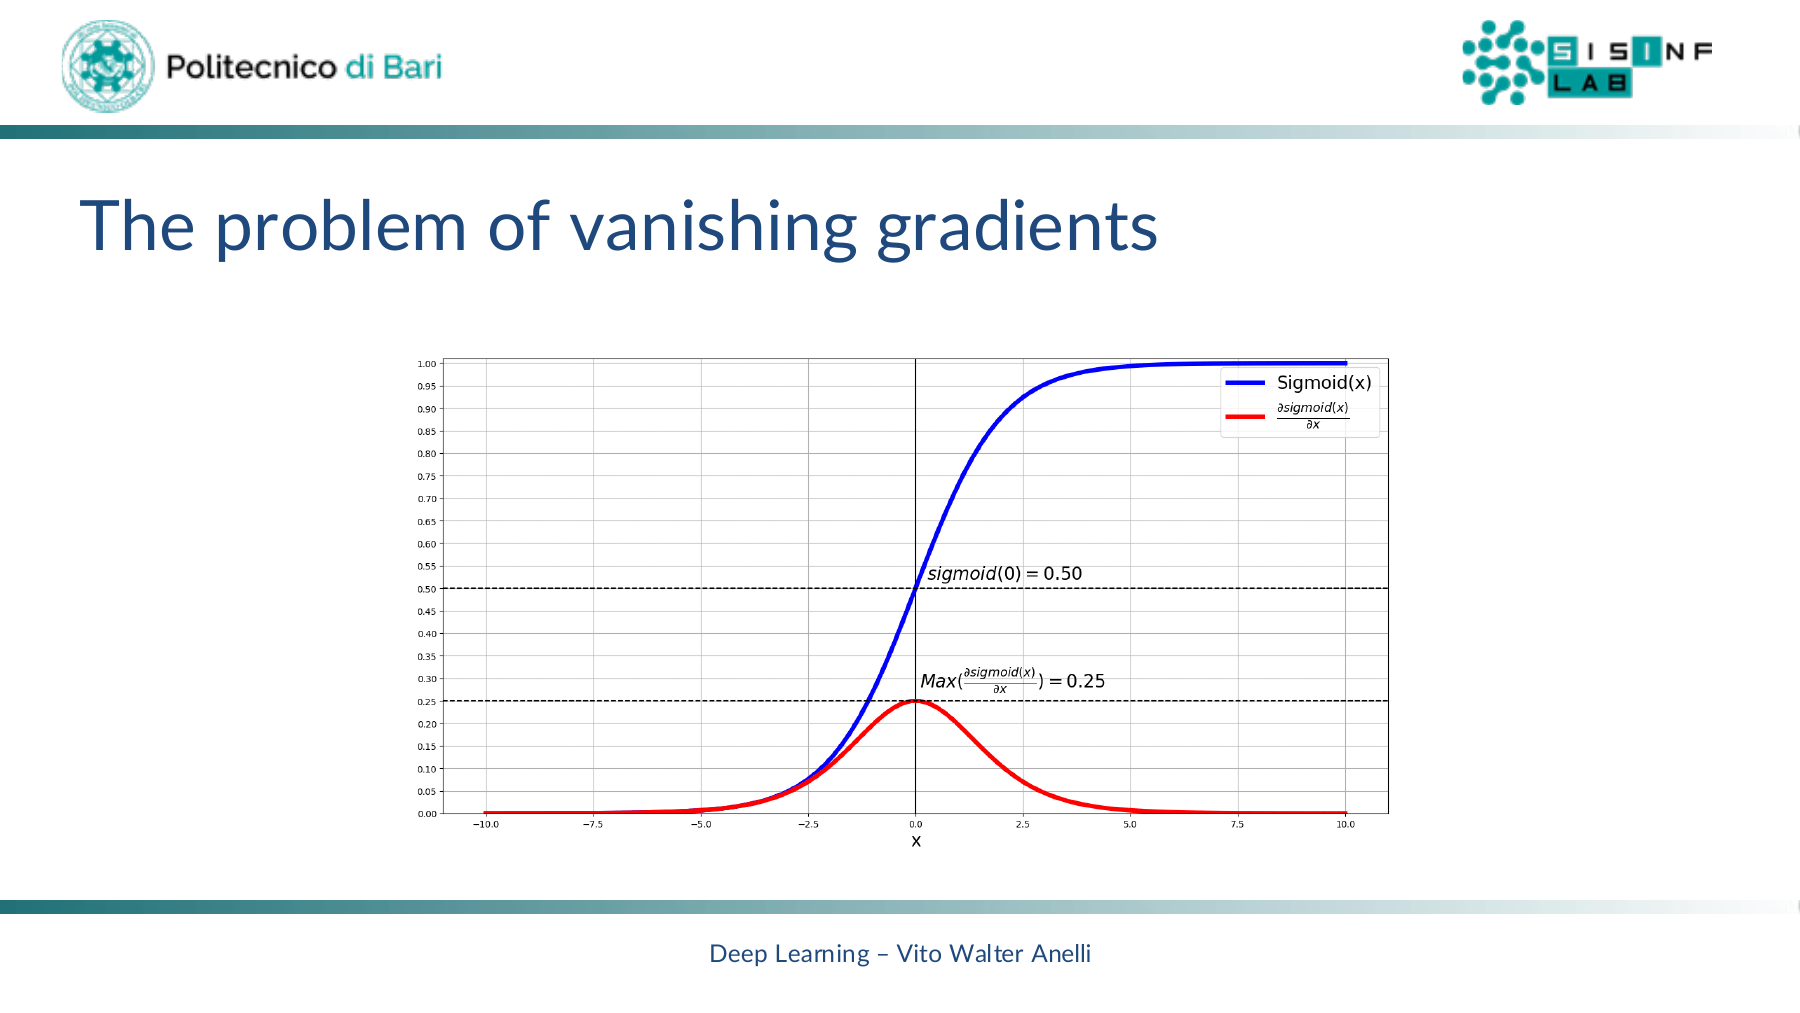
\includegraphics[width=0.82\linewidth]{figures/af03_vanishing_gradient.png}
  \caption{Sigmoid e sua derivata. Il valore $\sigma(0)=0{,}5$ è il punto di inflessione
           e il gradiente massimo è $0{,}25$. Per input molto grandi o molto piccoli
           la derivata tende a zero, bloccando il flusso del gradiente nei layer
           profondi.}
  \label{fig:vanishing_gradient}
\end{figure}

La soluzione più efficace è passare a funzioni \textbf{non saturanti} per i layer
interni, riservando funzioni saturanti solo all'output quando la struttura del
problema lo richiede (es.\ classificazione binaria, gating nelle LSTM).

%------------------------------------------------------------
\section{Panoramica: Saturating vs Non-Saturating}
\label{sec:overview-activations}

\begin{figure}[H]
  \centering
  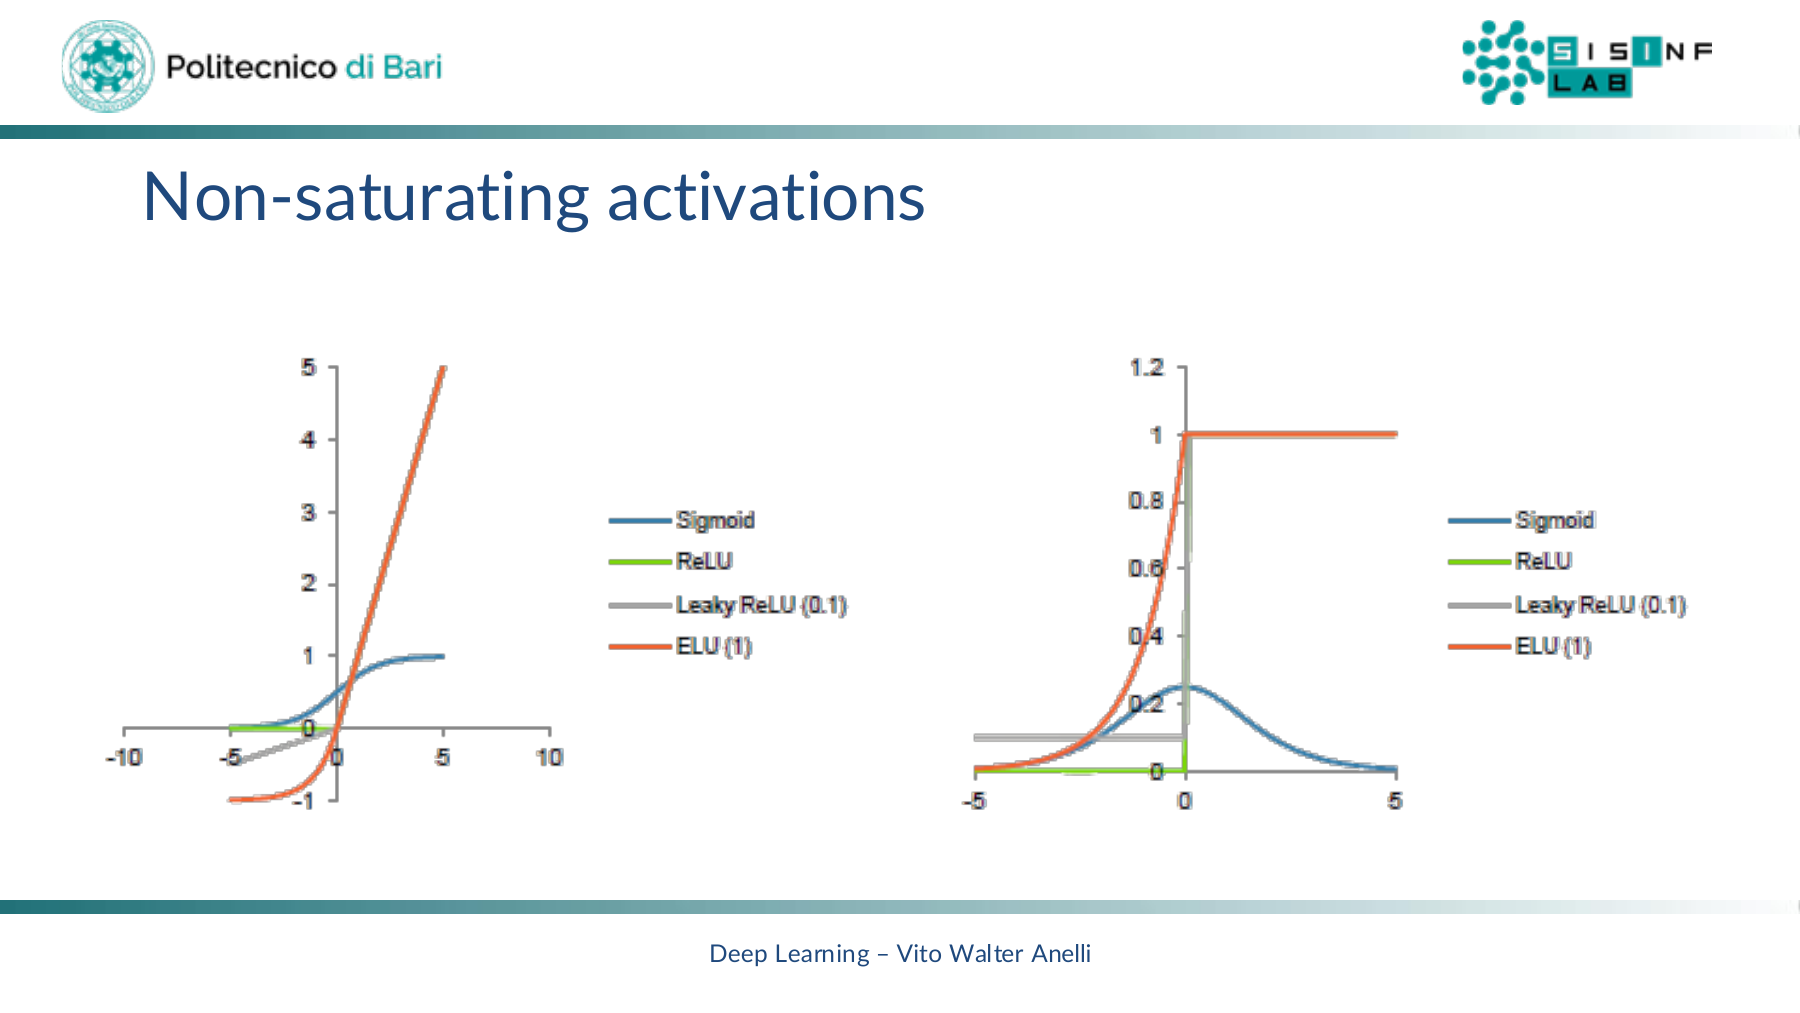
\includegraphics[width=0.90\linewidth]{figures/af03_nonsaturating_overview.png}
  \caption{Confronto visivo tra funzioni di attivazione saturanti e non saturanti
           (Sigmoid, ReLU, Leaky ReLU, ELU) nelle loro curve e nelle rispettive derivate.
           Le funzioni non saturanti mantengono un gradiente costante nella regione
           positiva, risolvendo il vanishing gradient.}
  \label{fig:nonsaturating_overview}
\end{figure}

%------------------------------------------------------------
\section{Famiglia ReLU}
\label{sec:relu-family}

\subsection{ReLU -- \texttt{nn.ReLU()}}
\label{subsec:relu}

La \textbf{Rectified Linear Unit} (ReLU) è oggi la funzione di attivazione di
default per i layer nascosti delle reti profonde \citep{bishop2024}:

\begin{equation}
  \operatorname{ReLU}(x) = (x)^{+} = \max(0, x).
\end{equation}

\begin{figure}[H]
  \centering
  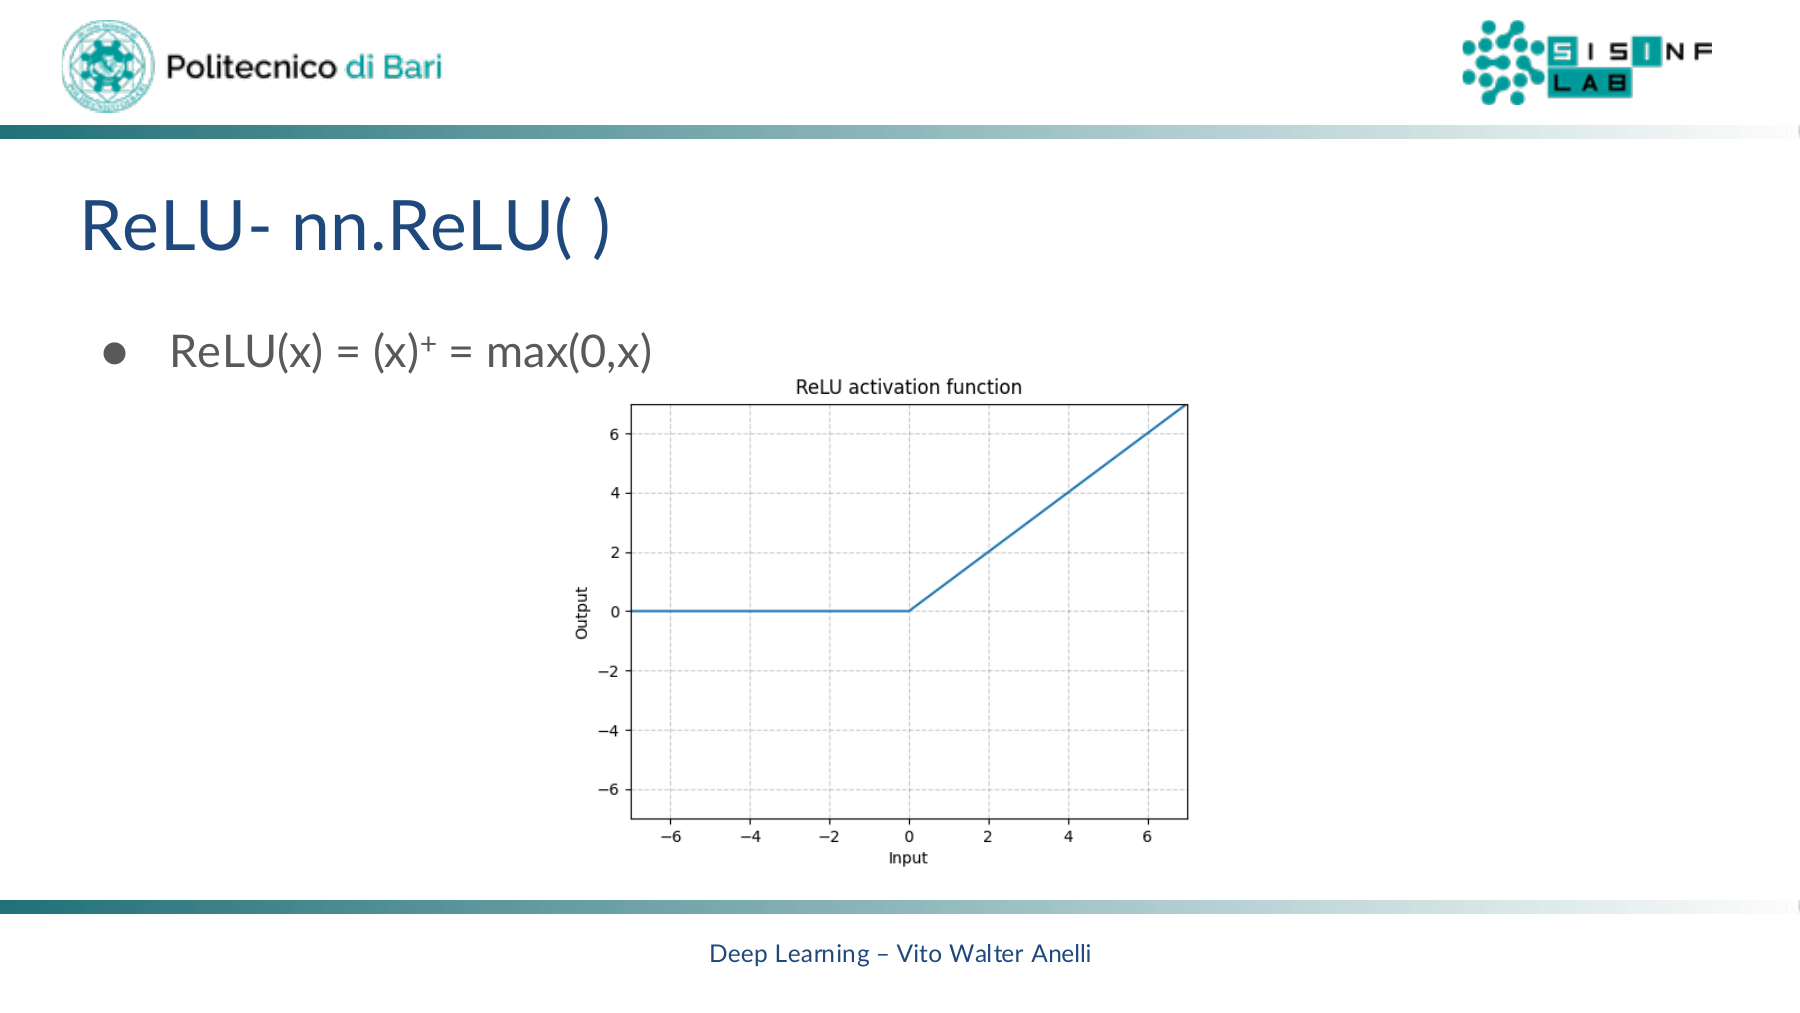
\includegraphics[width=0.72\linewidth]{figures/af03_relu.png}
  \caption{ReLU: uscita identità per $x \geq 0$, zero per $x < 0$.
           La derivata è discontinua in $x=0$ ma il gradiente è $1$ per tutti
           gli input positivi, eliminando completamente il vanishing gradient
           nel ramo attivo.}
  \label{fig:relu}
\end{figure}

\paragraph{Proprietà chiave.}
\begin{itemize}
  \item \textbf{Efficienza computazionale}: riduce a un semplice confronto con zero.
  \item \textbf{Gradiente non saturante}: la derivata è $1$ per $x>0$, evitando
        il vanishing gradient.
  \item \textbf{Sparsità}: i neuroni con input negativo producono esattamente zero,
        inducendo rappresentazioni sparse che migliorano la generalizzazione.
  \item \textbf{Dead ReLU problem}: se un neurone riceve input sempre negativi
        (es.\ dopo un grande aggiornamento del gradiente), il suo gradiente sarà
        sempre zero e il neurone cessa di apprendere. Le varianti seguenti
        mitigano questo problema.
\end{itemize}

\subsection{Leaky ReLU -- \texttt{nn.LeakyReLU()}}
\label{subsec:leaky-relu}

\begin{equation}
  \operatorname{LeakyReLU}(x) =
  \begin{cases}
    x,                                  & \text{se } x \geq 0 \\
    a_{\text{negative\_slope}} \times x, & \text{altrimenti}
  \end{cases}
\end{equation}

dove $a_{\text{negative\_slope}}$ è una piccola costante (tipicamente $0{,}01$).

\begin{figure}[H]
  \centering
  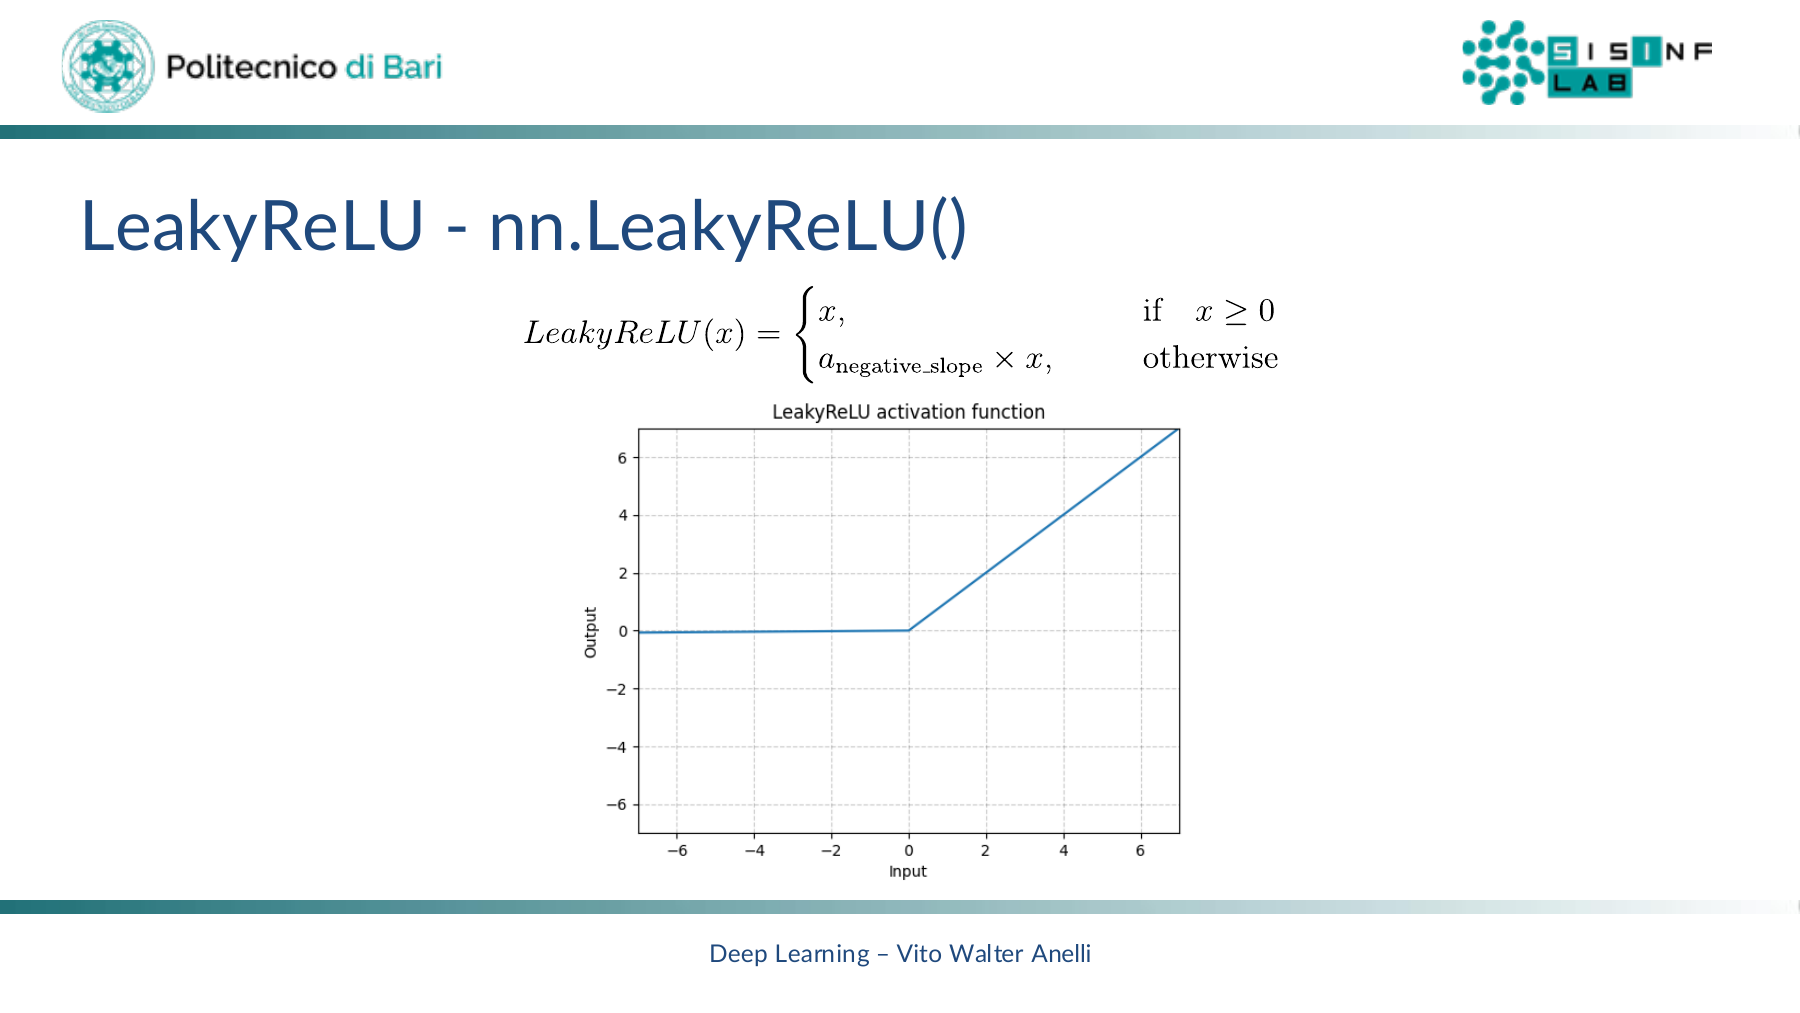
\includegraphics[width=0.72\linewidth]{figures/af03_leaky_relu.png}
  \caption{Leaky ReLU: introduce una piccola pendenza nella regione negativa
           ($a_{\text{neg}}=0{,}1$ nella figura), consentendo al gradiente di
           fluire anche per neuroni con input negativo e risolvendo il
           \emph{dead neuron} problem.}
  \label{fig:leaky_relu}
\end{figure}

Rispetto a ReLU, Leaky ReLU garantisce un gradiente non nullo anche per $x<0$,
mantenendo i neuroni attivi durante l'intero training.
Il coefficiente $a$ è fisso e scelto prima del training.

\subsection{PReLU -- \texttt{nn.PReLU()}}
\label{subsec:prelu}

\begin{equation}
  \operatorname{PReLU}(x) =
  \begin{cases}
    x,  & \text{se } x \geq 0 \\
    ax, & \text{altrimenti}
  \end{cases}
\end{equation}

\begin{figure}[H]
  \centering
  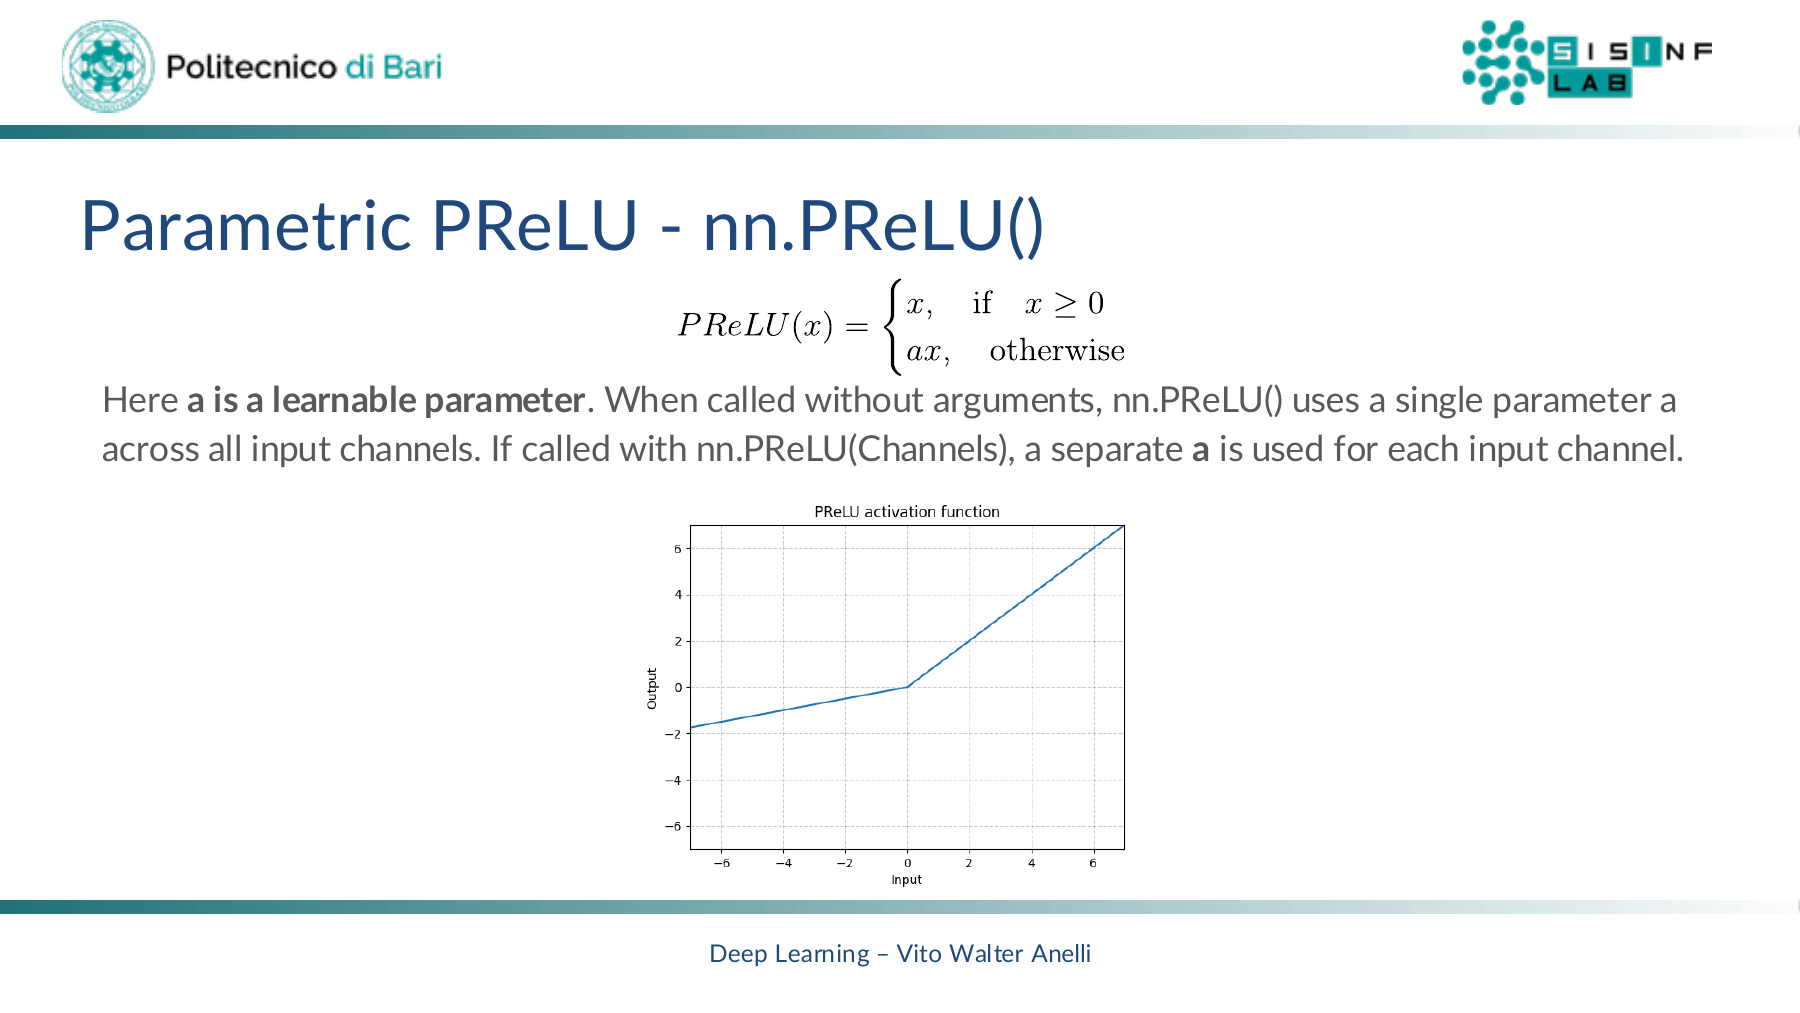
\includegraphics[width=0.72\linewidth]{figures/af03_prelu.png}
  \caption{Parametric ReLU (PReLU): il coefficiente $a$ è un \textbf{parametro
           apprendibile} con la retropropagazione. Chiamato senza argomenti,
           \texttt{nn.PReLU()} usa un unico parametro $a$ condiviso; chiamato
           con \texttt{nn.PReLU(C)}, usa un $a$ distinto per ognuno degli $C$
           canali in input.}
  \label{fig:prelu}
\end{figure}

La distinzione tra le tre varianti è riassumibile come segue:
\textbf{LReLU} usa un $a$ fisso, \textbf{PReLU} apprende $a$,
\textbf{RReLU} campiona $a$ casualmente durante il training.

\subsection{RReLU -- \texttt{nn.RReLU()}}
\label{subsec:rrelu}

\begin{equation}
  \operatorname{RReLU}(x) =
  \begin{cases}
    x,  & \text{se } x \geq 0 \\
    ax, & \text{altrimenti}
  \end{cases}
\end{equation}

\begin{figure}[H]
  \centering
  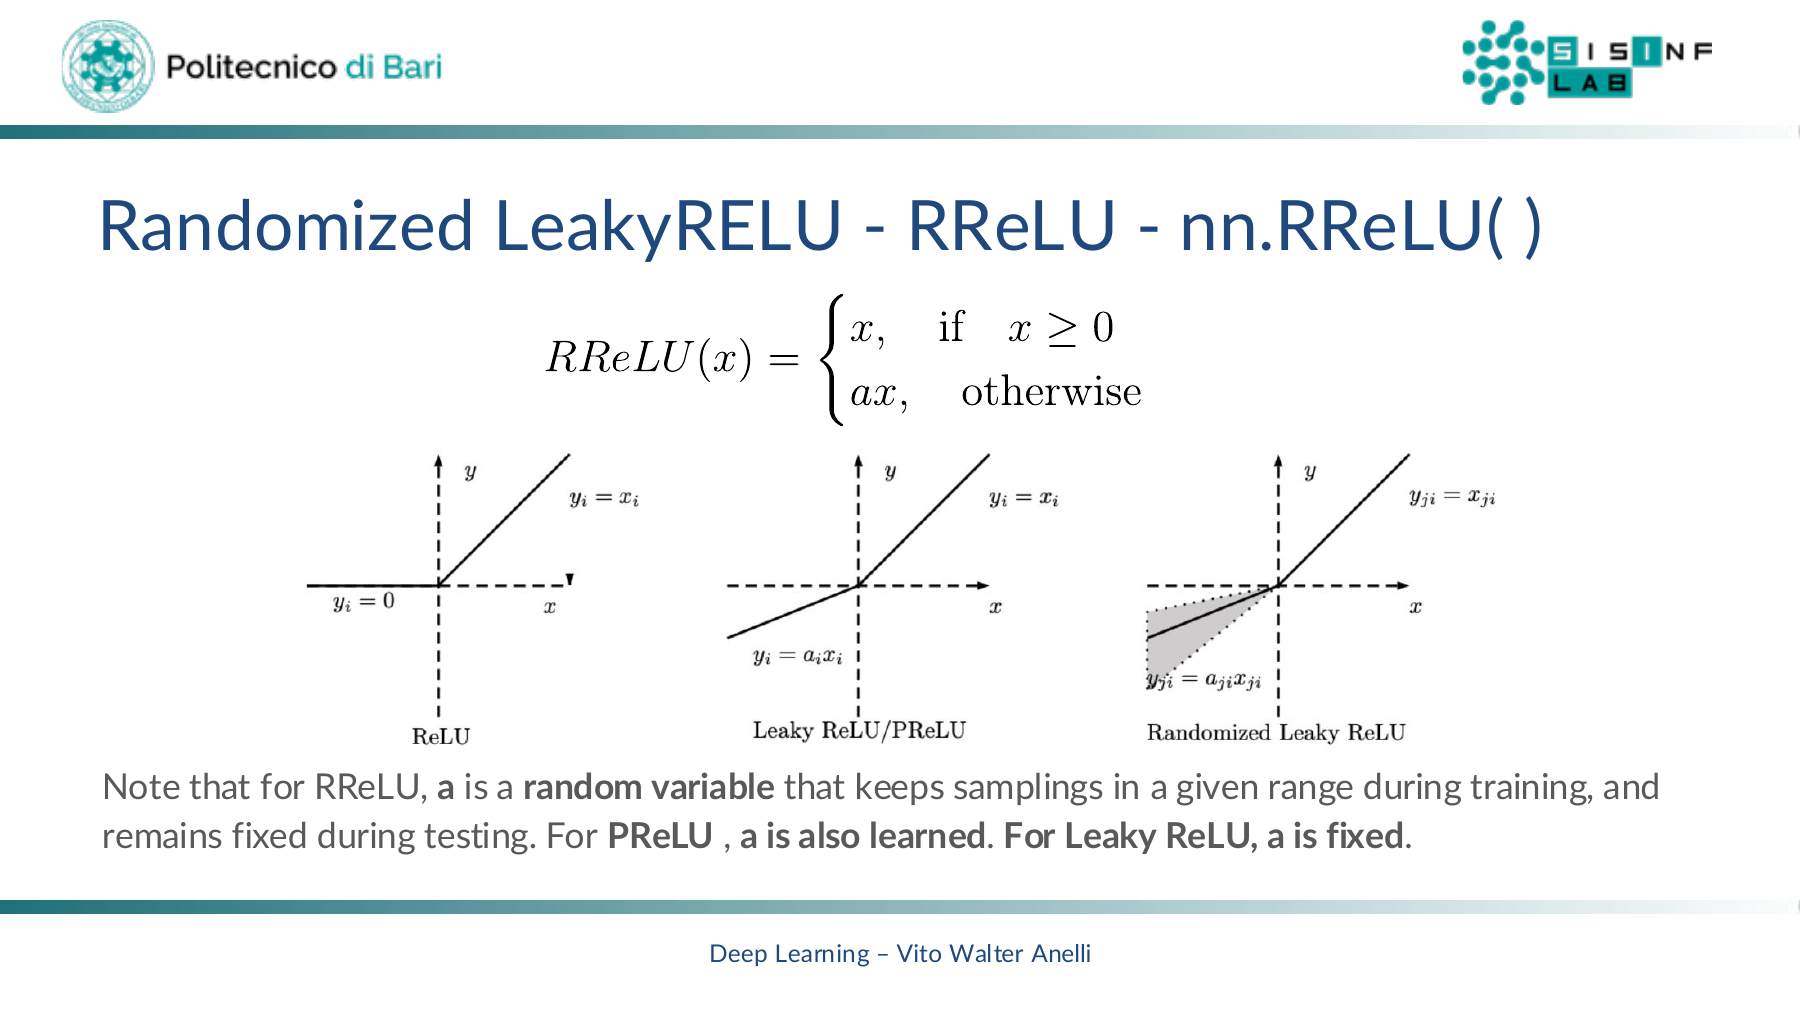
\includegraphics[width=0.85\linewidth]{figures/af03_rrelu.png}
  \caption{Confronto visivo tra ReLU, Leaky ReLU/PReLU e Randomized Leaky ReLU (RReLU).
           In RReLU, il parametro $a_{ji}$ è campionato uniformemente da un intervallo
           $[l,u]$ durante il training; al test viene usato il valor medio $(l+u)/2$.
           Questo effetto di randomizzazione funge da regolarizzazione implicita.}
  \label{fig:rrelu}
\end{figure}

\begin{figure}[H]
  \centering
  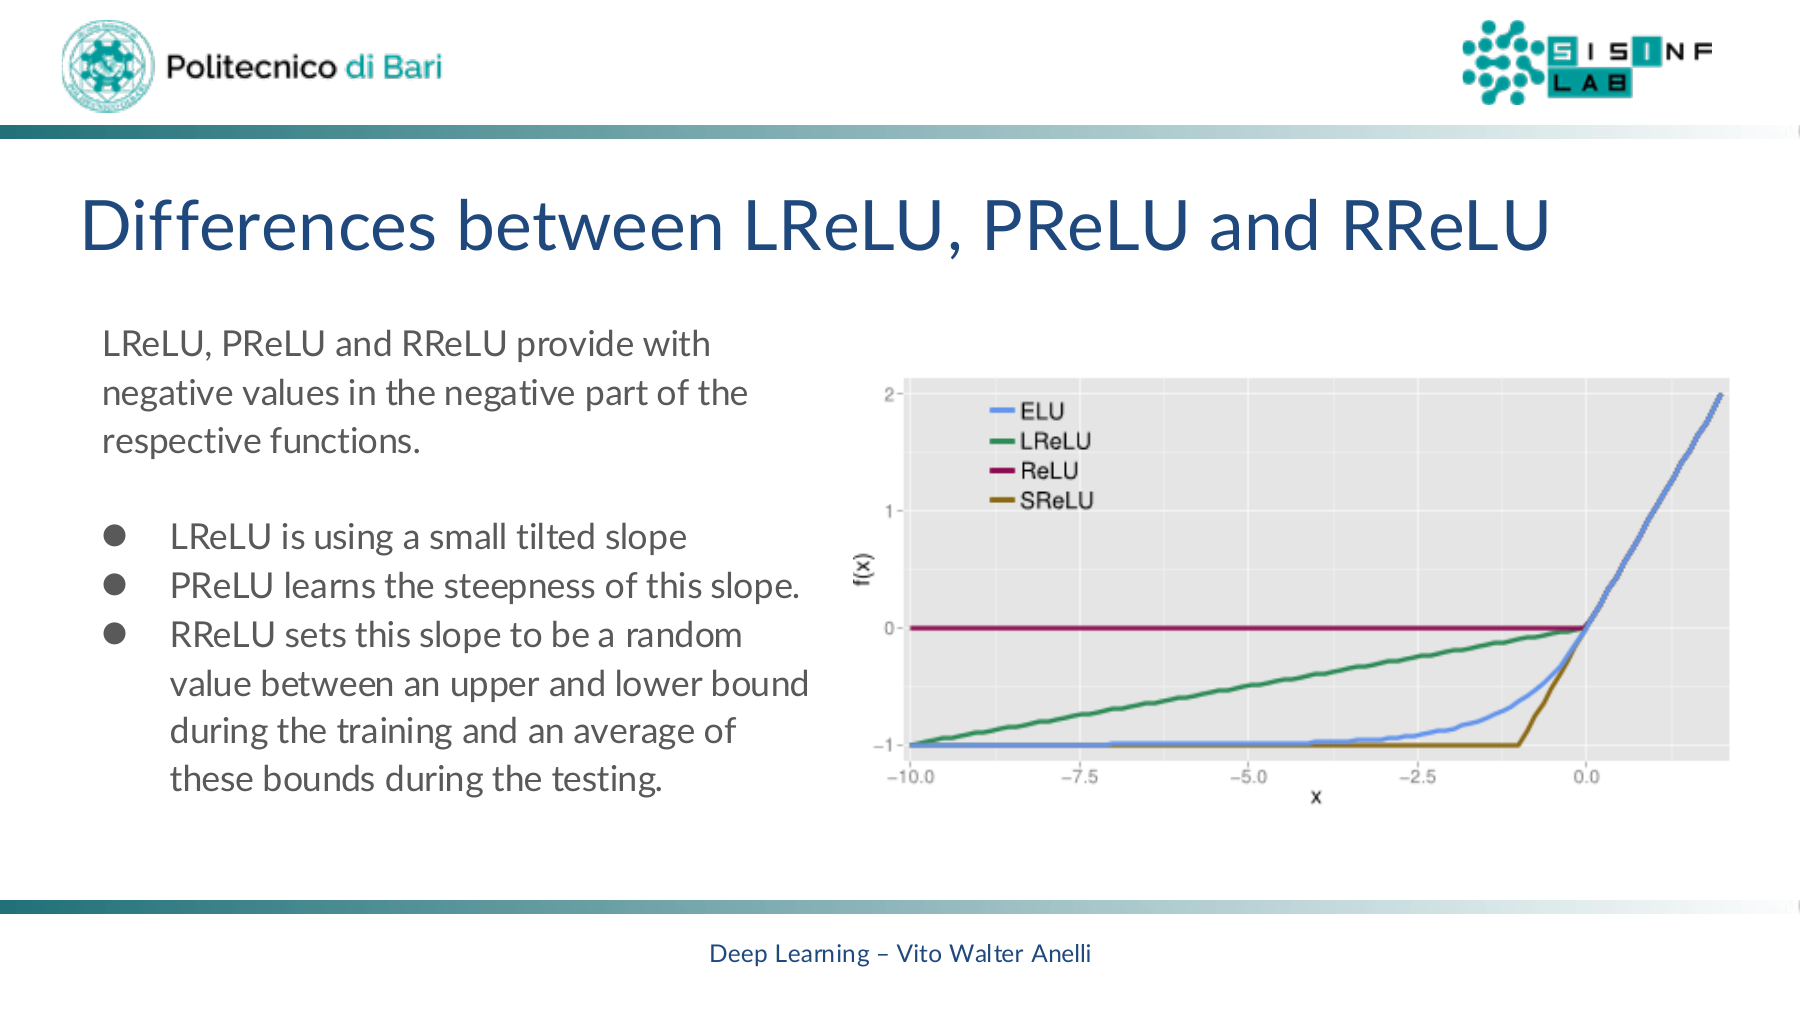
\includegraphics[width=0.80\linewidth]{figures/af03_lrelu_prelu_rrelu_diff.png}
  \caption{Differenze nella regione negativa tra ELU, LReLU, ReLU e SReLU.
           LReLU usa una pendenza fissa piccola; PReLU la apprende; RReLU
           la randomizza durante il training e la fissa alla media al test.}
  \label{fig:lrelu_prelu_rrelu_diff}
\end{figure}

\subsection{ReLU6 -- \texttt{nn.ReLU6()}}
\label{subsec:relu6}

\begin{equation}
  \operatorname{ReLU6}(x) = \min\!\bigl(\max(0, x),\, 6\bigr).
\end{equation}

\begin{figure}[H]
  \centering
  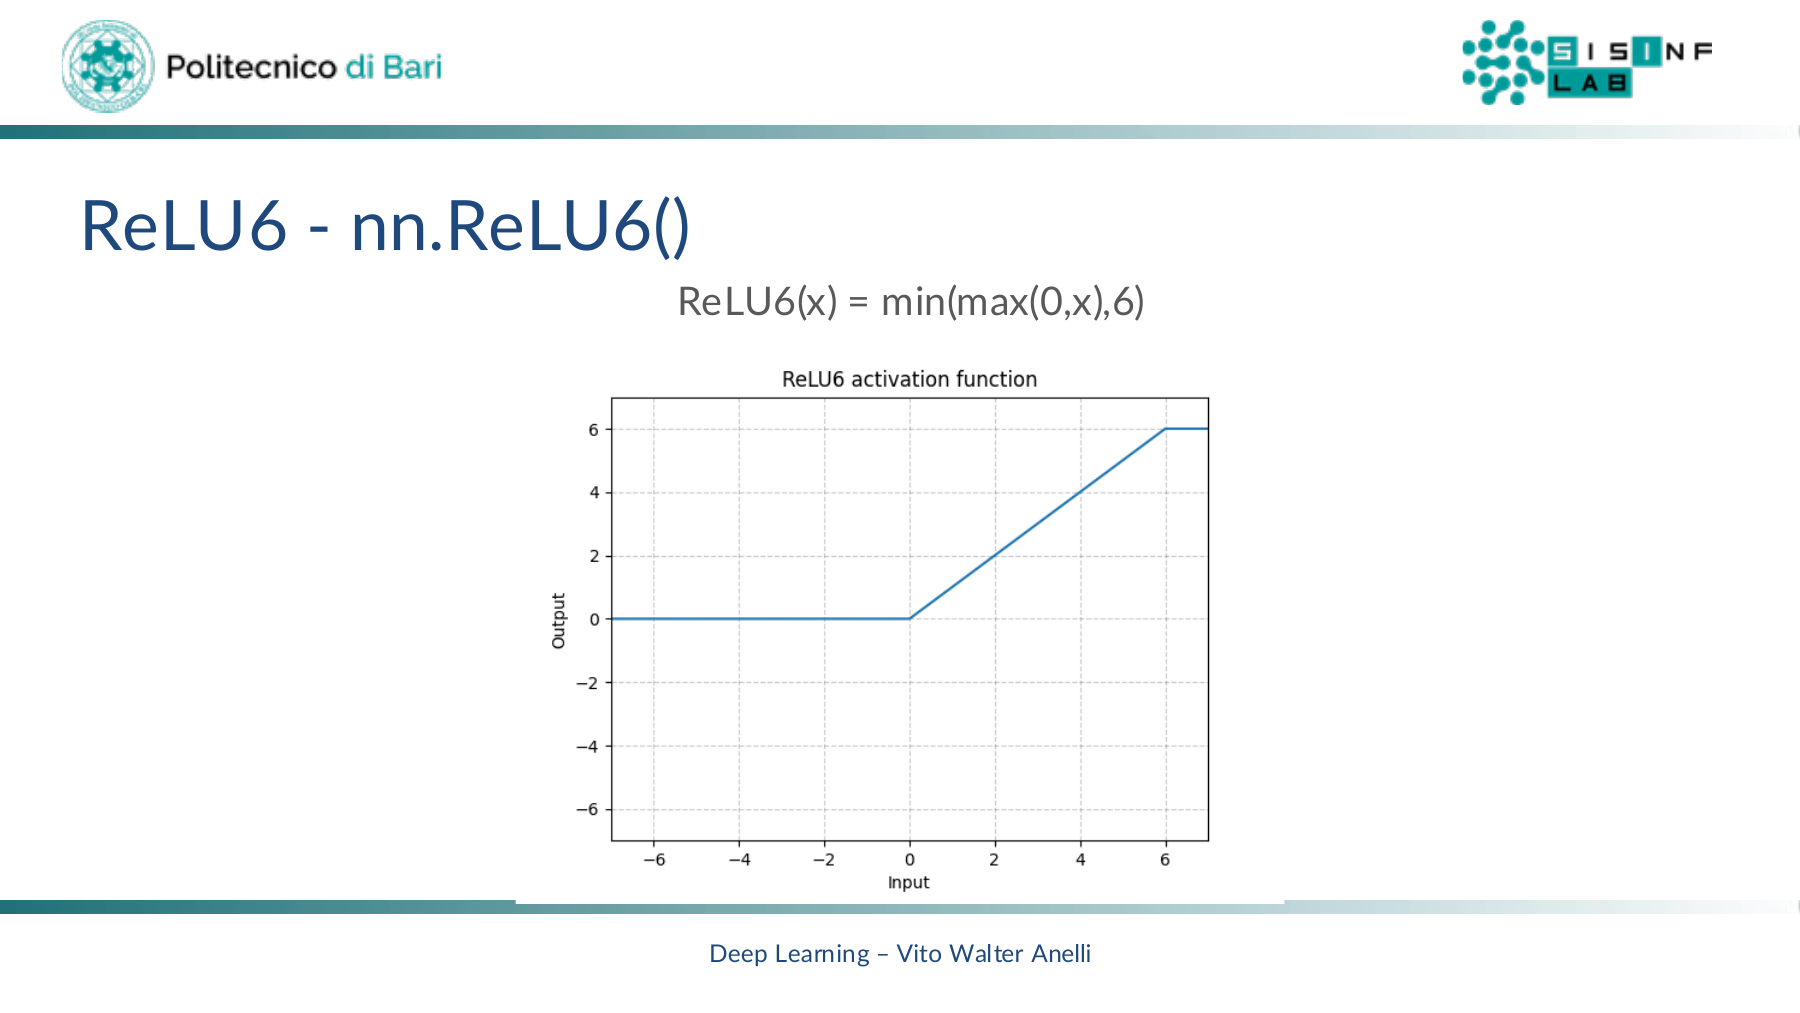
\includegraphics[width=0.72\linewidth]{figures/af03_relu6.png}
  \caption{ReLU6: ReLU con saturazione superiore a $6$. Progettata
           per ambienti a precisione ridotta (es.\ mobile/quantizzazione),
           previene attivazioni molto grandi che possono degradare la
           rappresentazione in virgola mobile a bassa precisione.}
  \label{fig:relu6}
\end{figure}

%------------------------------------------------------------
\section{Famiglia ELU}
\label{sec:elu-family}

\subsection{ELU -- \texttt{nn.ELU()}}
\label{subsec:elu}

La \textbf{Exponential Linear Unit} risolve sia il dead neuron problem sia il
problema delle medie non centrate in zero \citep{bishop2024}:

\begin{equation}
  \operatorname{ELU}(x) = \max(0,x) + \min\!\bigl(0,\, \alpha\cdot(\exp(x)-1)\bigr).
\end{equation}

\begin{figure}[H]
  \centering
  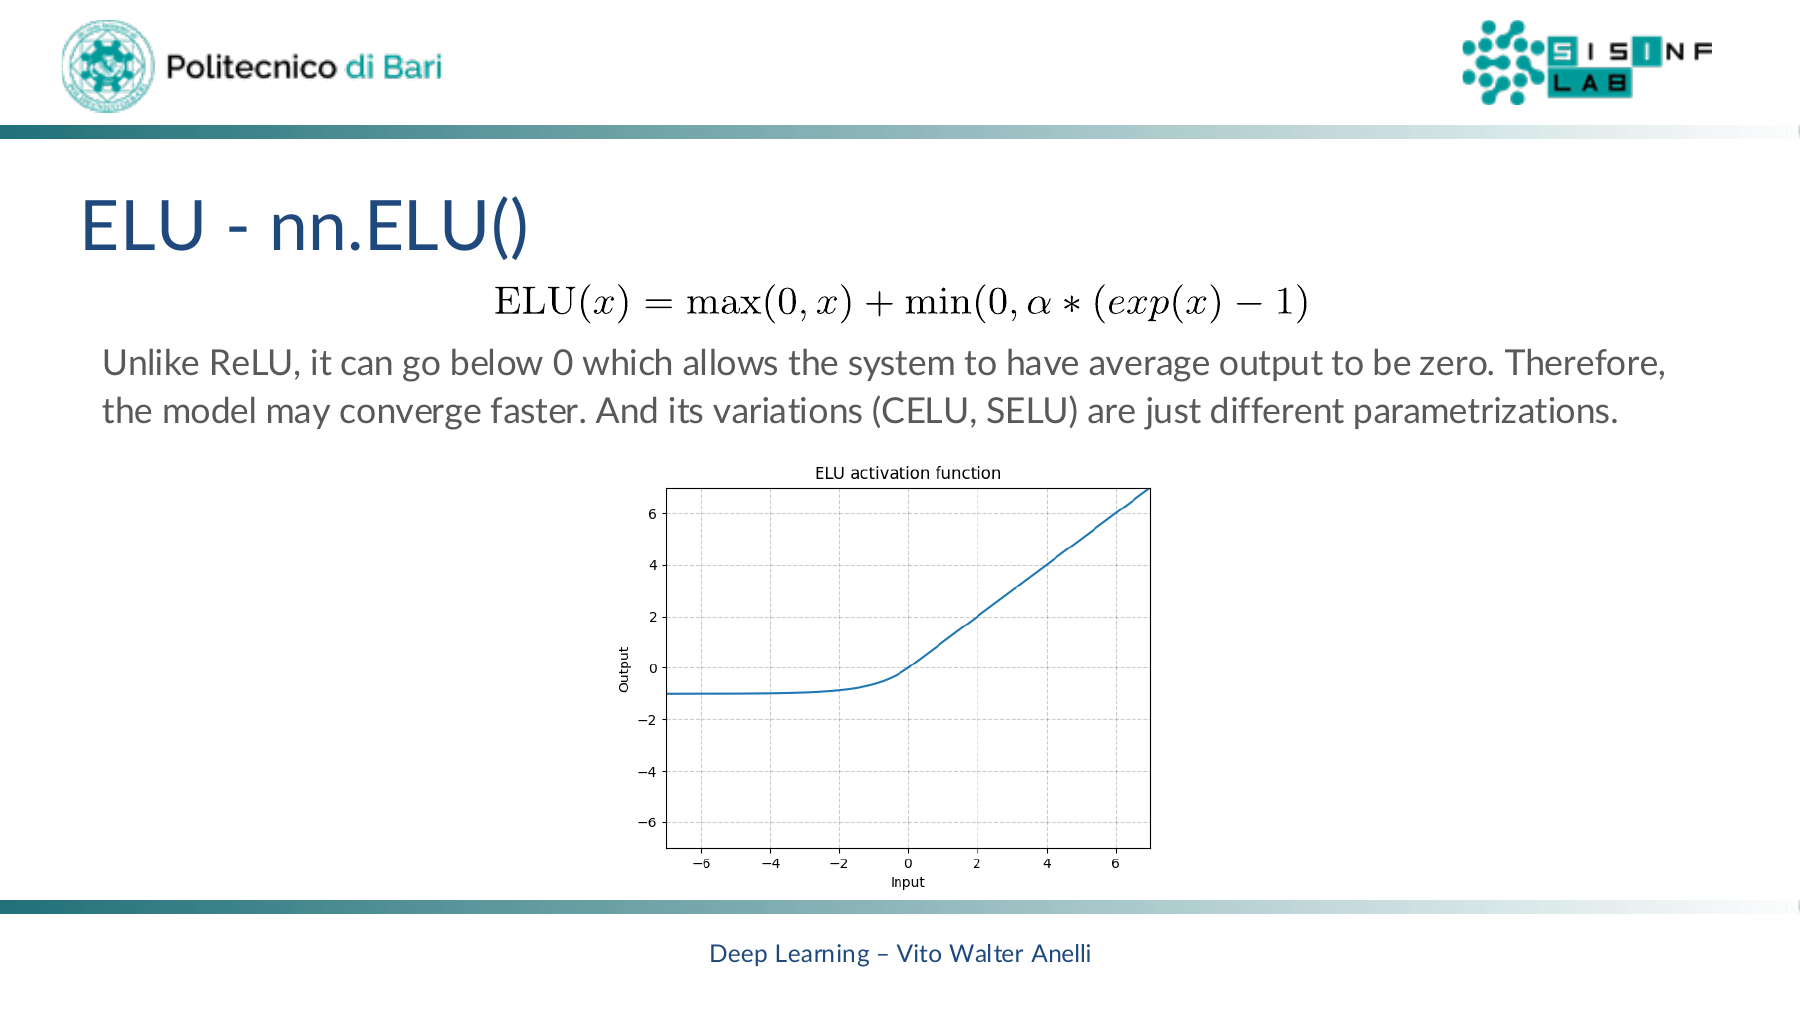
\includegraphics[width=0.72\linewidth]{figures/af03_elu.png}
  \caption{ELU: a differenza di ReLU, può produrre valori negativi,
           permettendo all'output medio del layer di essere vicino a zero.
           Questo centra le attivazioni e accelera la convergenza.
           Le varianti CELU e SELU sono reparametrizzazioni di ELU.}
  \label{fig:elu}
\end{figure}

Il valore $\alpha$ controlla il limite inferiore della regione negativa
(di default $\alpha = 1$). Avere output con media vicina a zero ha lo stesso
beneficio del \emph{Batch Normalization}: il gradiente non è sistematicamente
distorto, e la convergenza è più rapida.

\subsection{CELU -- \texttt{nn.CELU()}}
\label{subsec:celu}

\begin{equation}
  \operatorname{CELU}(x) = \max(0,x) + \min\!\left(0,\, \alpha \cdot
  \left(\exp\!\left(\frac{x}{\alpha}\right) - 1\right)\right).
\end{equation}

\begin{figure}[H]
  \centering
  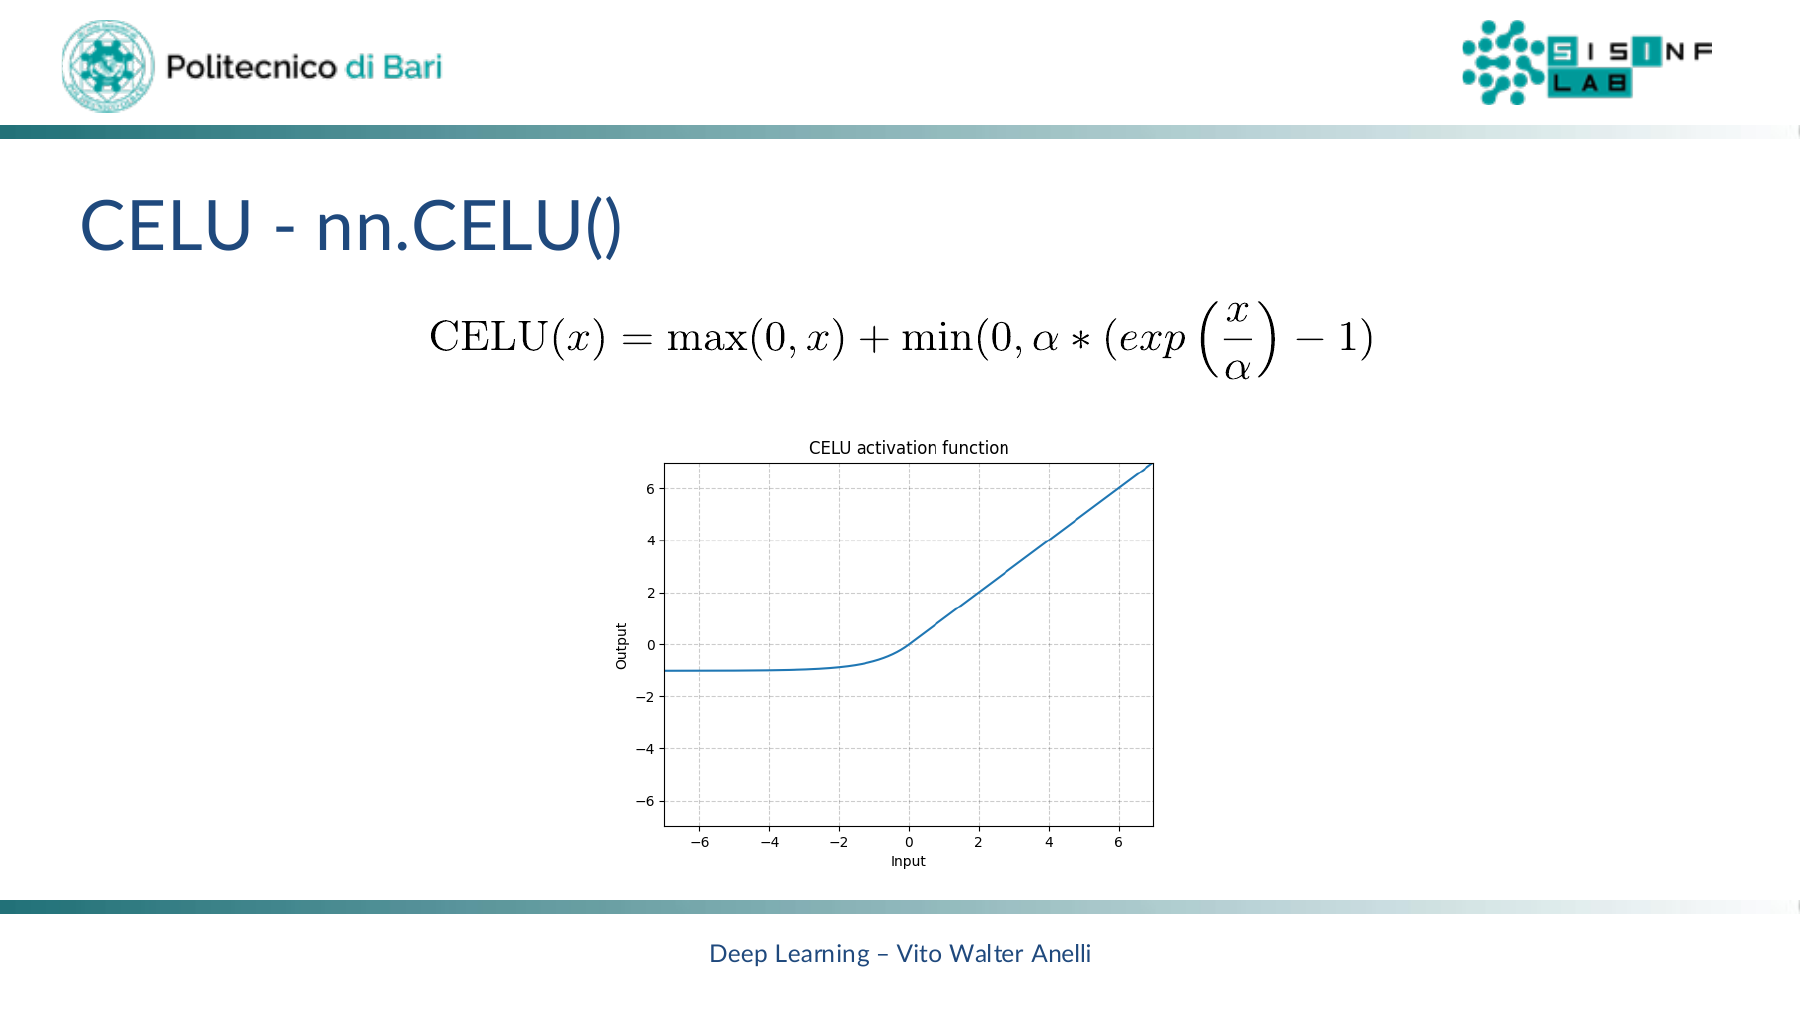
\includegraphics[width=0.72\linewidth]{figures/af03_celu.png}
  \caption{CELU (Continuously Differentiable ELU): reparametrizza ELU in modo
           da garantire la derivabilità continua in $x=0$ per qualsiasi valore
           di $\alpha$, migliorando la stabilità numerica del training.}
  \label{fig:celu}
\end{figure}

\subsection{SELU -- \texttt{nn.SELU()}}
\label{subsec:selu}

\begin{equation}
  \operatorname{SELU}(x) = \mathrm{scale} \cdot
  \bigl(\max(0,x) + \min\!\bigl(0,\,\alpha\cdot(\exp(x)-1)\bigr)\bigr),
\end{equation}
con $\mathrm{scale} \approx 1{,}0507$ e $\alpha \approx 1{,}6733$
(valori calcolati analiticamente da Klambauer et al., 2017).

\begin{figure}[H]
  \centering
  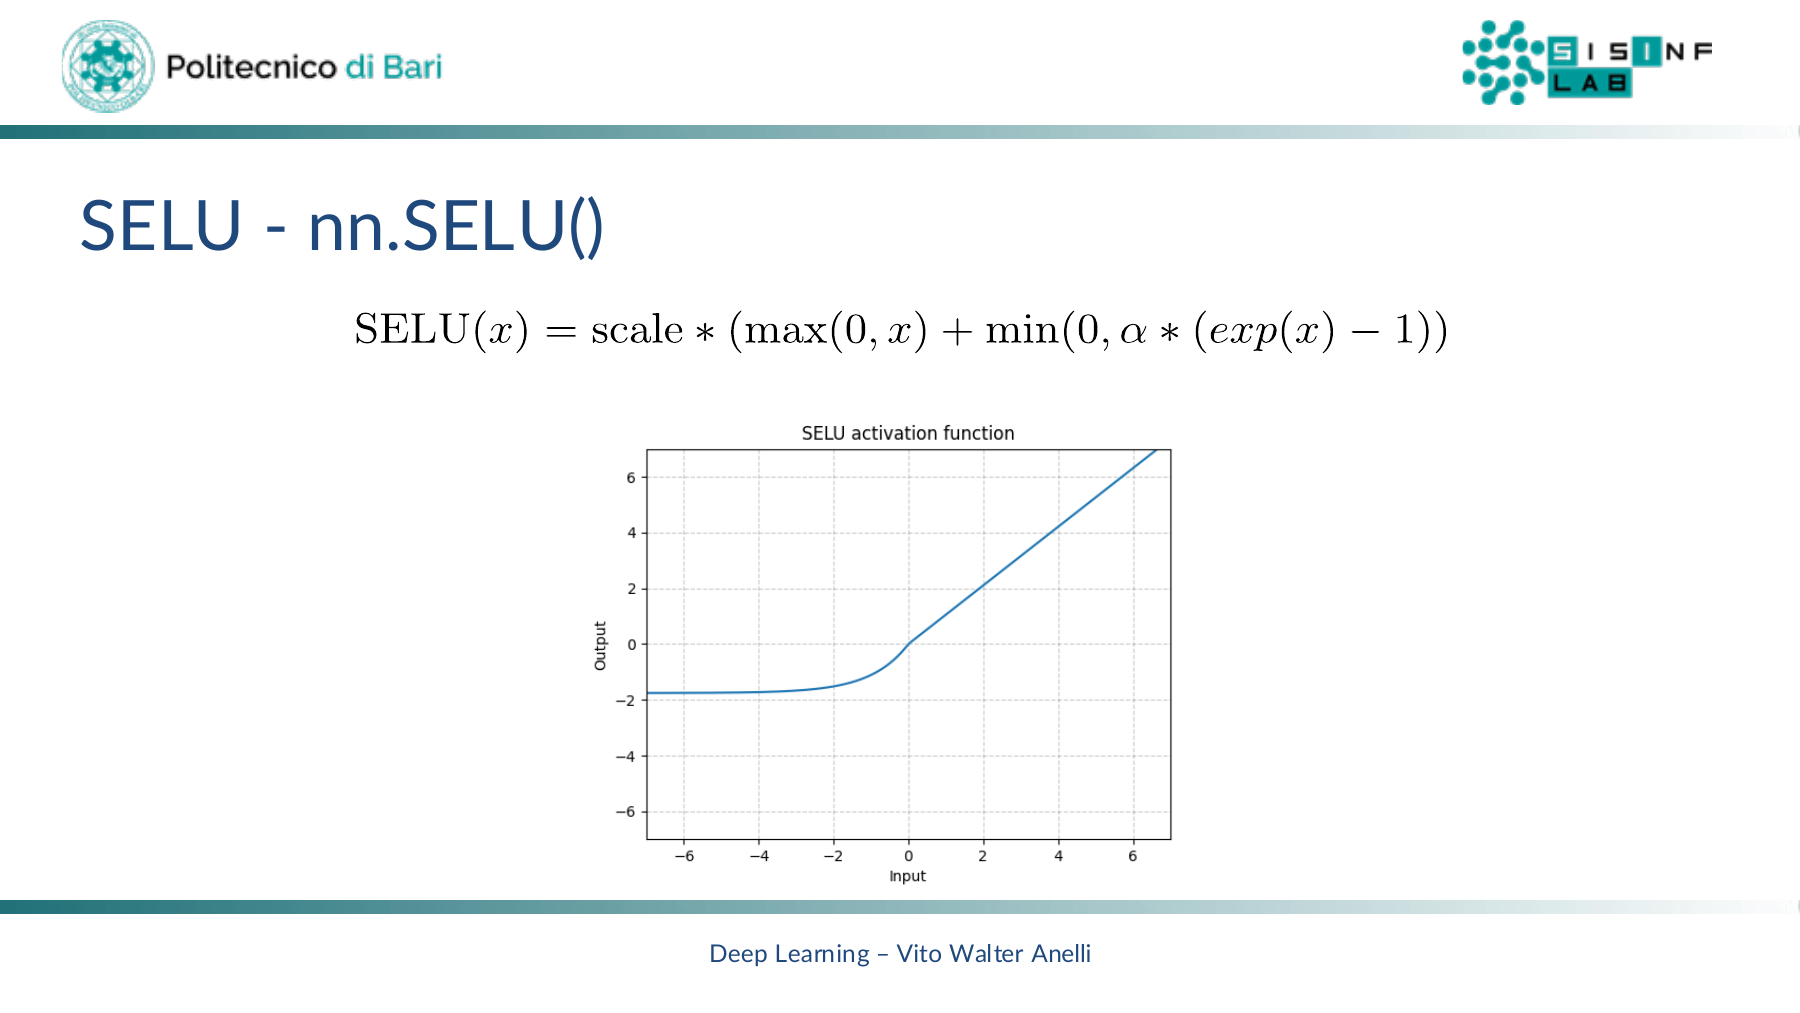
\includegraphics[width=0.72\linewidth]{figures/af03_selu.png}
  \caption{SELU (Scaled ELU): aggiunge un fattore di scala alla ELU.
           Con le costanti $\alpha$ e \emph{scale} opportune, la SELU garantisce
           \emph{self-normalizing} properties: attivazioni con media $0$ e
           varianza $1$ si propagano stabili attraverso layer arbitrariamente
           profondi, senza necessità di Batch Normalization.}
  \label{fig:selu}
\end{figure}

%------------------------------------------------------------
\section{Softplus e GELU}
\label{sec:softplus-gelu}

\subsection{Softplus -- \texttt{nn.Softplus()}}
\label{subsec:softplus}

\begin{equation}
  \operatorname{Softplus}(x) = \frac{1}{\beta} \cdot \log\!\bigl(1 + \exp(\beta x)\bigr).
\end{equation}

\begin{figure}[H]
  \centering
  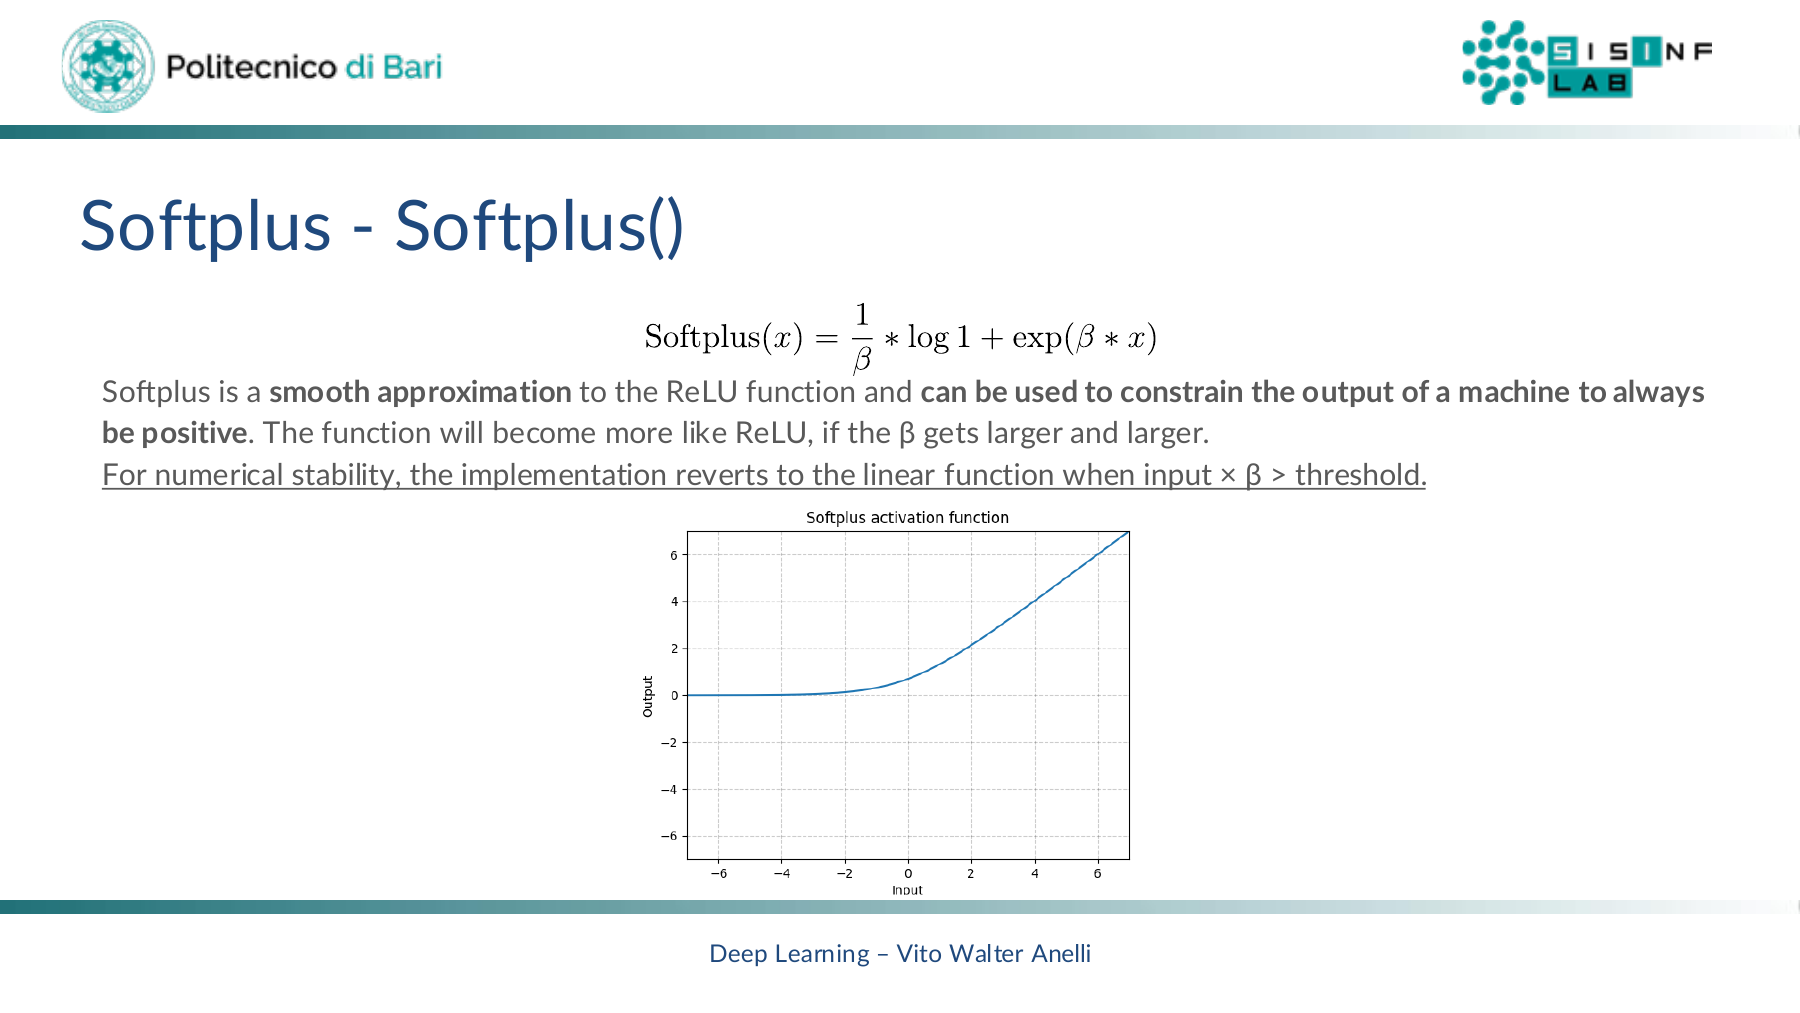
\includegraphics[width=0.72\linewidth]{figures/af03_softplus.png}
  \caption{Softplus: approssimazione \textbf{smooth} di ReLU, con derivata continua
           in tutto $\mathbb{R}$. All'aumentare di $\beta$ converge a ReLU.
           Può essere usata per \emph{vincolare l'output a essere sempre positivo}.
           Per stabilità numerica, l'implementazione torna alla funzione lineare
           quando $x \cdot \beta > \mathrm{threshold}$.}
  \label{fig:softplus}
\end{figure}

La Softplus è la primitiva della Sigmoid: $\frac{d}{dx}\operatorname{Softplus}(x) = \sigma(x)$,
il che ne chiarisce il ruolo teorico come ``versione continua'' di ReLU.

\subsection{GELU -- \texttt{nn.GELU()}}
\label{subsec:gelu}

\begin{equation}
  \operatorname{GELU}(x) = x \cdot \Phi(x),
\end{equation}
dove $\Phi(x)$ è la \emph{Cumulative Distribution Function} della distribuzione gaussiana standard.

\begin{figure}[H]
  \centering
  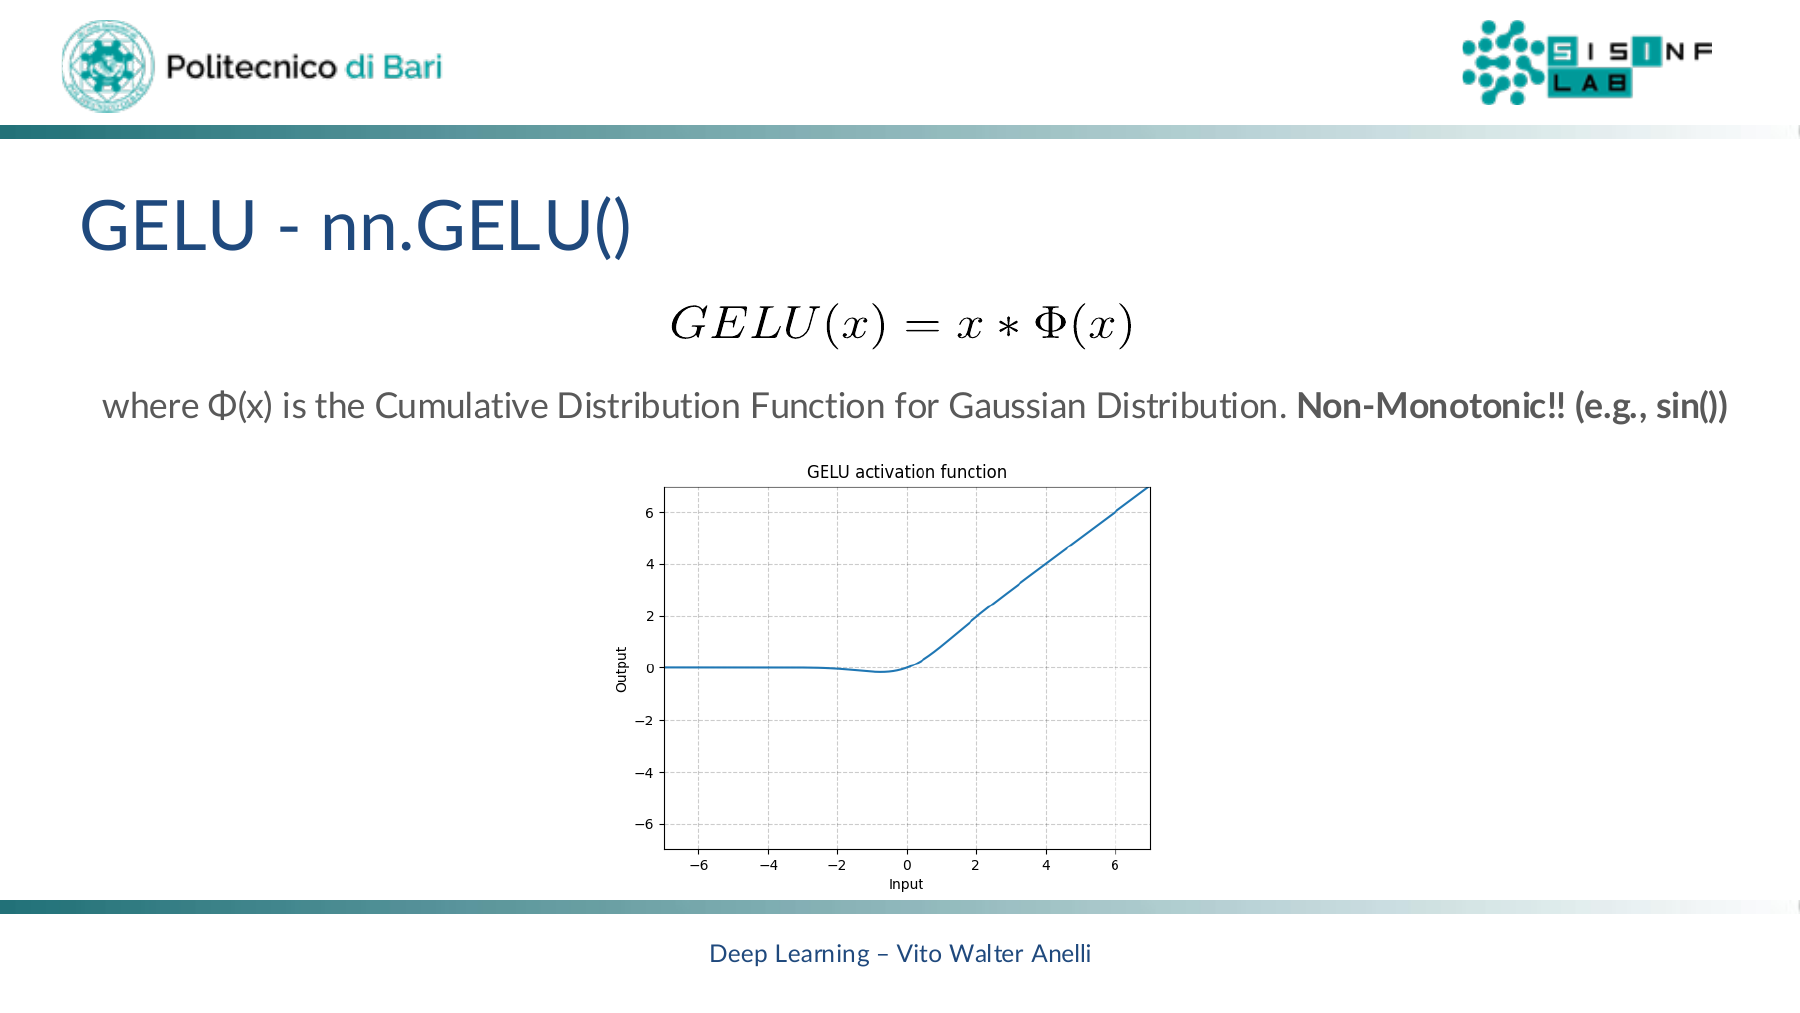
\includegraphics[width=0.72\linewidth]{figures/af03_gelu.png}
  \caption{GELU (Gaussian Error Linear Unit): funzione \textbf{non monotona},
           a differenza di ReLU e delle sue varianti. Nella regione $x < 0$
           l'output decresce, poi risale, imitando il comportamento del dropout
           stocastico. È la funzione di attivazione predefinita nei Transformer
           (BERT, GPT) per le sue proprietà di regolarizzazione implicita.}
  \label{fig:gelu}
\end{figure}

L'approssimazione pratica spesso utilizzata è:
\begin{equation}
  \operatorname{GELU}(x) \approx 0{,}5\, x
  \left(1 + \tanh\!\left[\sqrt{\frac{2}{\pi}}\bigl(x + 0{,}044715\, x^3\bigr)\right]\right).
\end{equation}

%------------------------------------------------------------
\section{Funzioni Saturanti}
\label{sec:saturating}

\subsection{Sigmoid -- \texttt{nn.Sigmoid()}}
\label{subsec:sigmoid}

\begin{equation}
  \operatorname{Sigmoid}(x) = \sigma(x) = \frac{1}{1 + \exp(-x)}.
\end{equation}

\begin{figure}[H]
  \centering
  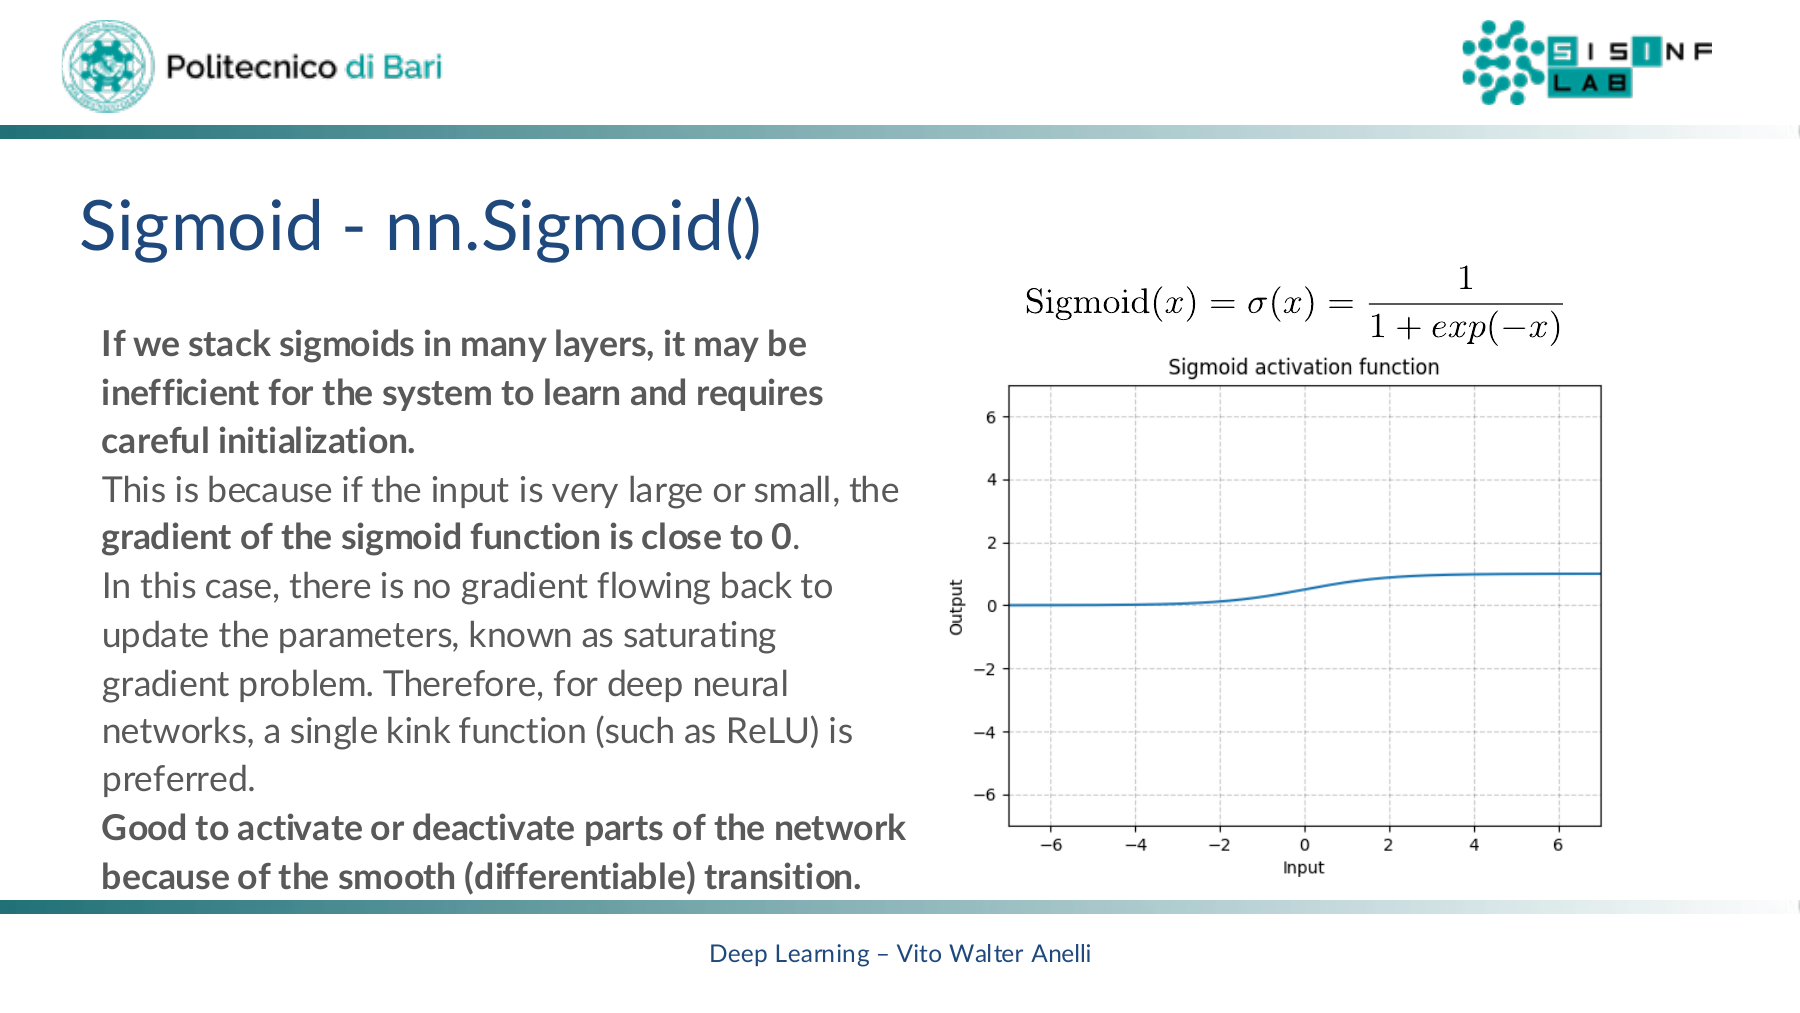
\includegraphics[width=0.85\linewidth]{figures/af03_sigmoid.png}
  \caption{Sigmoid: output in $(0,1)$, il che la rende ideale come gate
           (LSTM, GRU) o per output probabilistici di classificatori binari.
           Impilare molti layer sigmoid causa il vanishing gradient: il gradiente
           della sigmoid è prossimo a zero per $|x| \gg 0$, bloccando la
           retropropagazione. Per reti profonde si preferisce ReLU.}
  \label{fig:sigmoid}
\end{figure}

\paragraph{Connessione con Softmax.}
Come mostrato nelle slide (Sez.~\ref{sec:softmax}), la Sigmoid è un caso
speciale della Softmax a due classi: posto $x_2 = 0$,
\begin{equation}
  z_1 = \frac{e^{x_1}}{e^{x_1}+e^{x_2}}
      = \frac{e^{x_1}}{e^{x_1}+1}
      = \frac{1}{1+e^{-x_1}} = \sigma(x_1).
\end{equation}

\subsection{Tanh -- \texttt{nn.Tanh()}}
\label{subsec:tanh}

\begin{equation}
  \operatorname{Tanh}(x) = \tanh(x) = \frac{\exp(x) - \exp(-x)}{\exp(x) + \exp(-x)}.
\end{equation}

\begin{figure}[H]
  \centering
  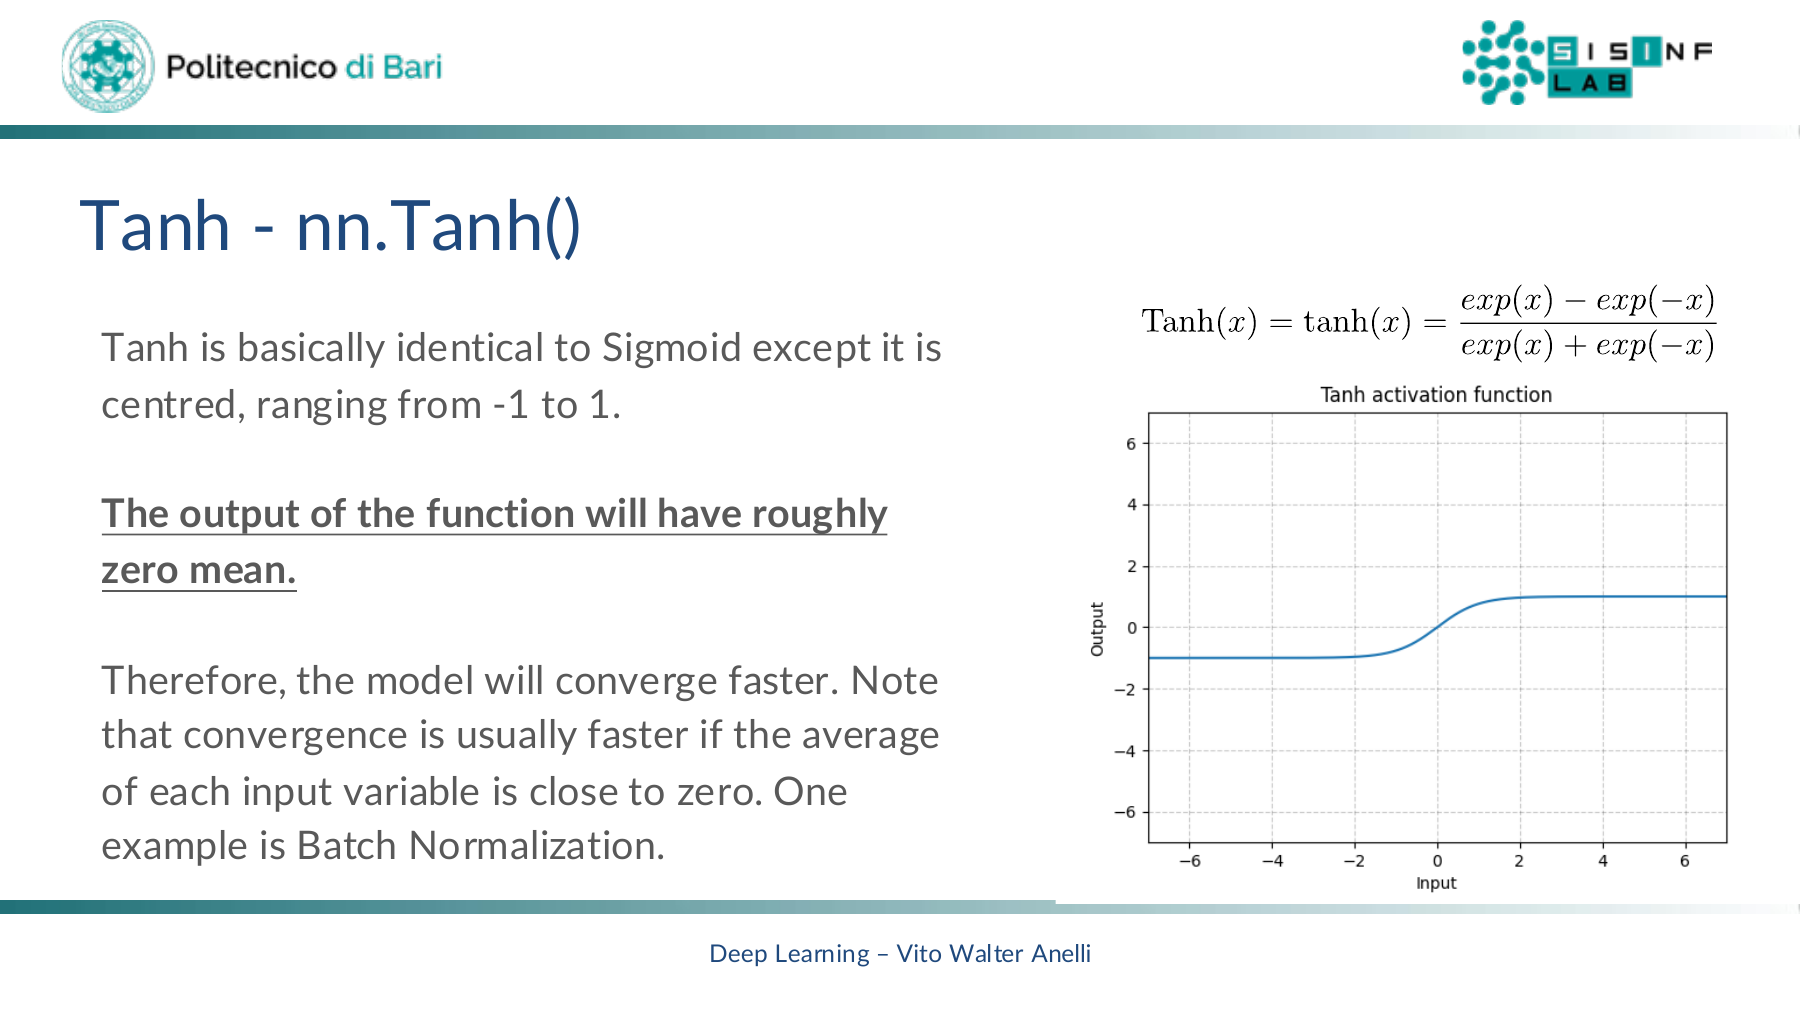
\includegraphics[width=0.85\linewidth]{figures/af03_tanh.png}
  \caption{Tanh: versione centrata della Sigmoid con output in $(-1, 1)$.
           L'output ha media approssimativamente zero, accelerando la convergenza
           rispetto a Sigmoid (nota fondamentale: la convergenza è più rapida
           quando la media degli input è vicina a zero, come avviene nel
           Batch Normalization). Soffre comunque del vanishing gradient.}
  \label{fig:tanh}
\end{figure}

\paragraph{Relazione con Sigmoid.}
$\tanh(x) = 2\sigma(2x) - 1$: Tanh è semplicemente una Sigmoid riscalata e
traslata. Preferire Tanh a Sigmoid nei layer nascosti perché l'output centrato
evita bias sistematici nel gradiente \citep{bishop2024}.

\subsection{Hardtanh -- \texttt{nn.Hardtanh()}}
\label{subsec:hardtanh}

\begin{equation}
  \operatorname{Hardtanh}(x) =
  \begin{cases}
    1,  & \text{se } x > 1 \\
    -1, & \text{se } x < -1 \\
    x,  & \text{altrimenti}
  \end{cases}
\end{equation}

\begin{figure}[H]
  \centering
  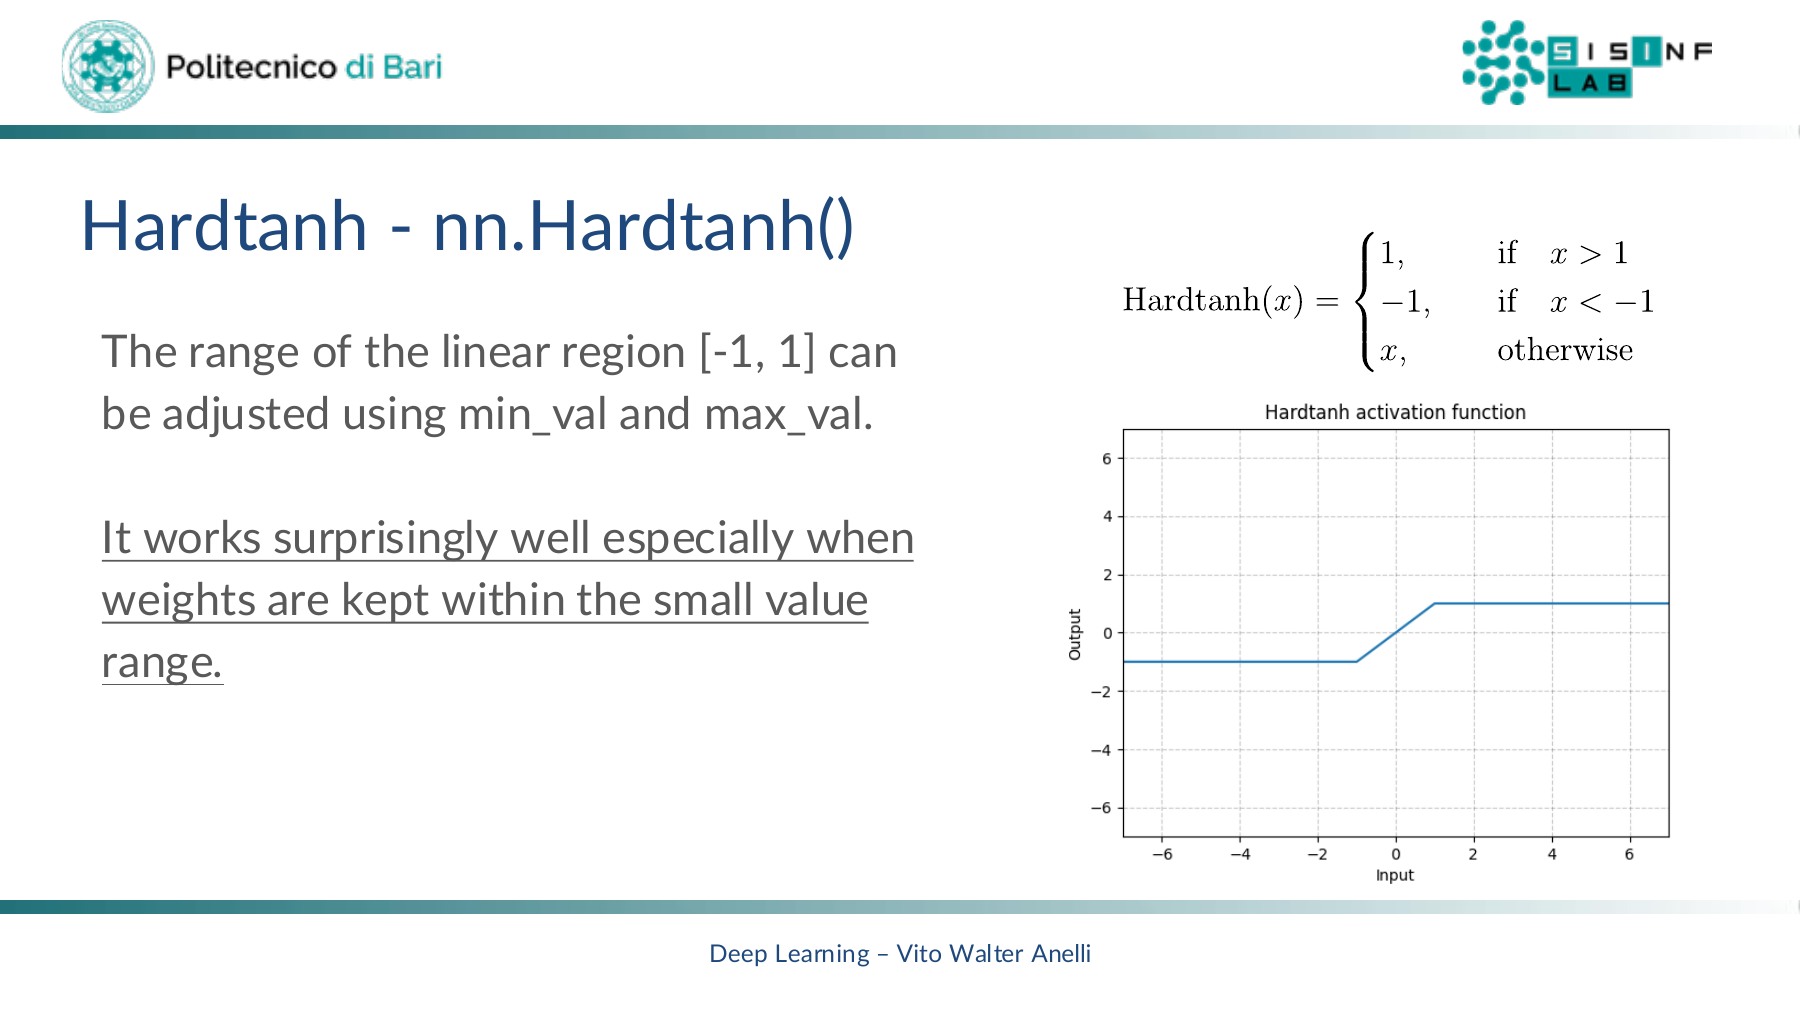
\includegraphics[width=0.85\linewidth]{figures/af03_hardtanh.png}
  \caption{Hardtanh: approssimazione lineare a tratti di Tanh.
           I valori di saturazione $[-1, 1]$ sono regolabili tramite
           \texttt{min\_val} e \texttt{max\_val}. Funziona sorprendentemente
           bene quando i pesi rimangono in un range di valori piccoli, ed è
           computazionalmente più leggera di Tanh.}
  \label{fig:hardtanh}
\end{figure}

\subsection{Softsign -- \texttt{nn.Softsign()}}
\label{subsec:softsign}

\begin{equation}
  \operatorname{SoftSign}(x) = \frac{x}{1 + |x|}.
\end{equation}

\begin{figure}[H]
  \centering
  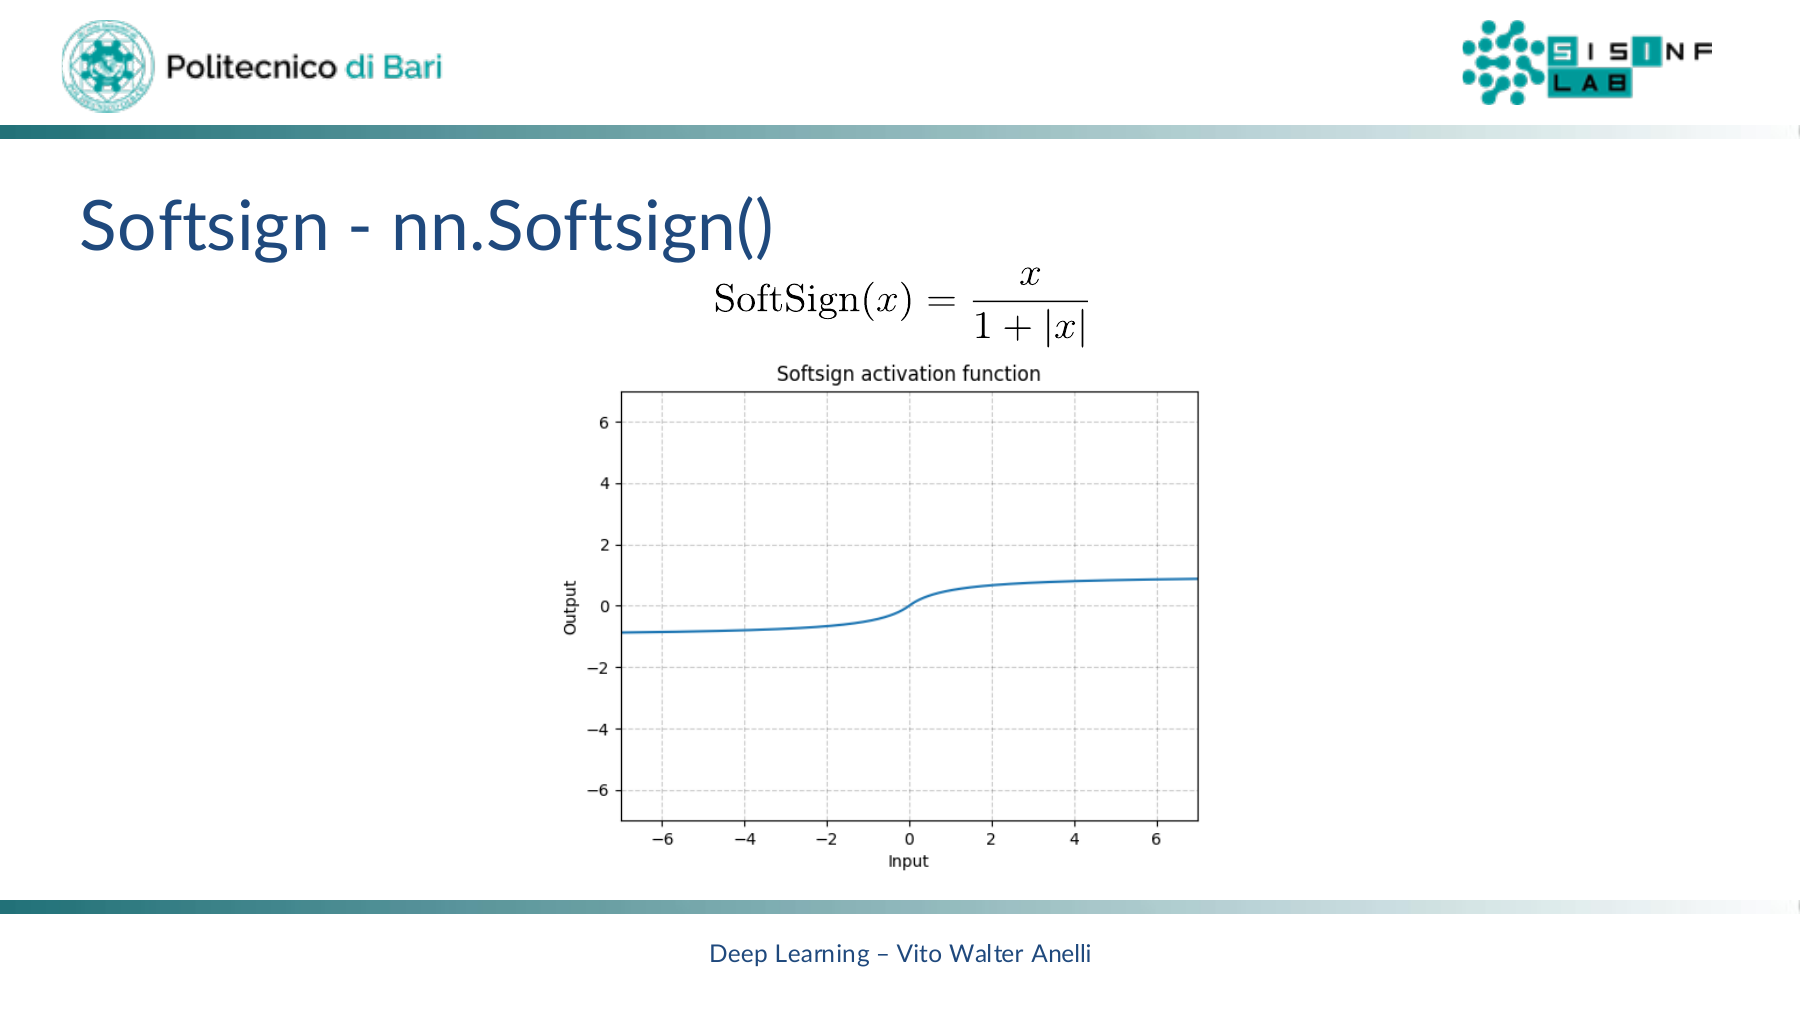
\includegraphics[width=0.72\linewidth]{figures/af03_softsign.png}
  \caption{Softsign: alternativa a Tanh con saturazione più lenta
           (decadimento polinomiale anziché esponenziale). Le code più
           pesanti implicano gradienti meno soggetti al vanishing problem
           rispetto a Tanh, ma l'output rimane in $(-1,1)$.}
  \label{fig:softsign}
\end{figure}

%------------------------------------------------------------
\section{Funzioni Shrink e Threshold}
\label{sec:shrink-threshold}

\subsection{Threshold -- \texttt{nn.Threshold()}}
\label{subsec:threshold}

\begin{equation}
  \operatorname{threshold}(x) =
  \begin{cases}
    x, & \text{se } x > \mathrm{threshold} \\
    v, & \text{altrimenti}
  \end{cases}
\end{equation}

\begin{figure}[H]
  \centering
  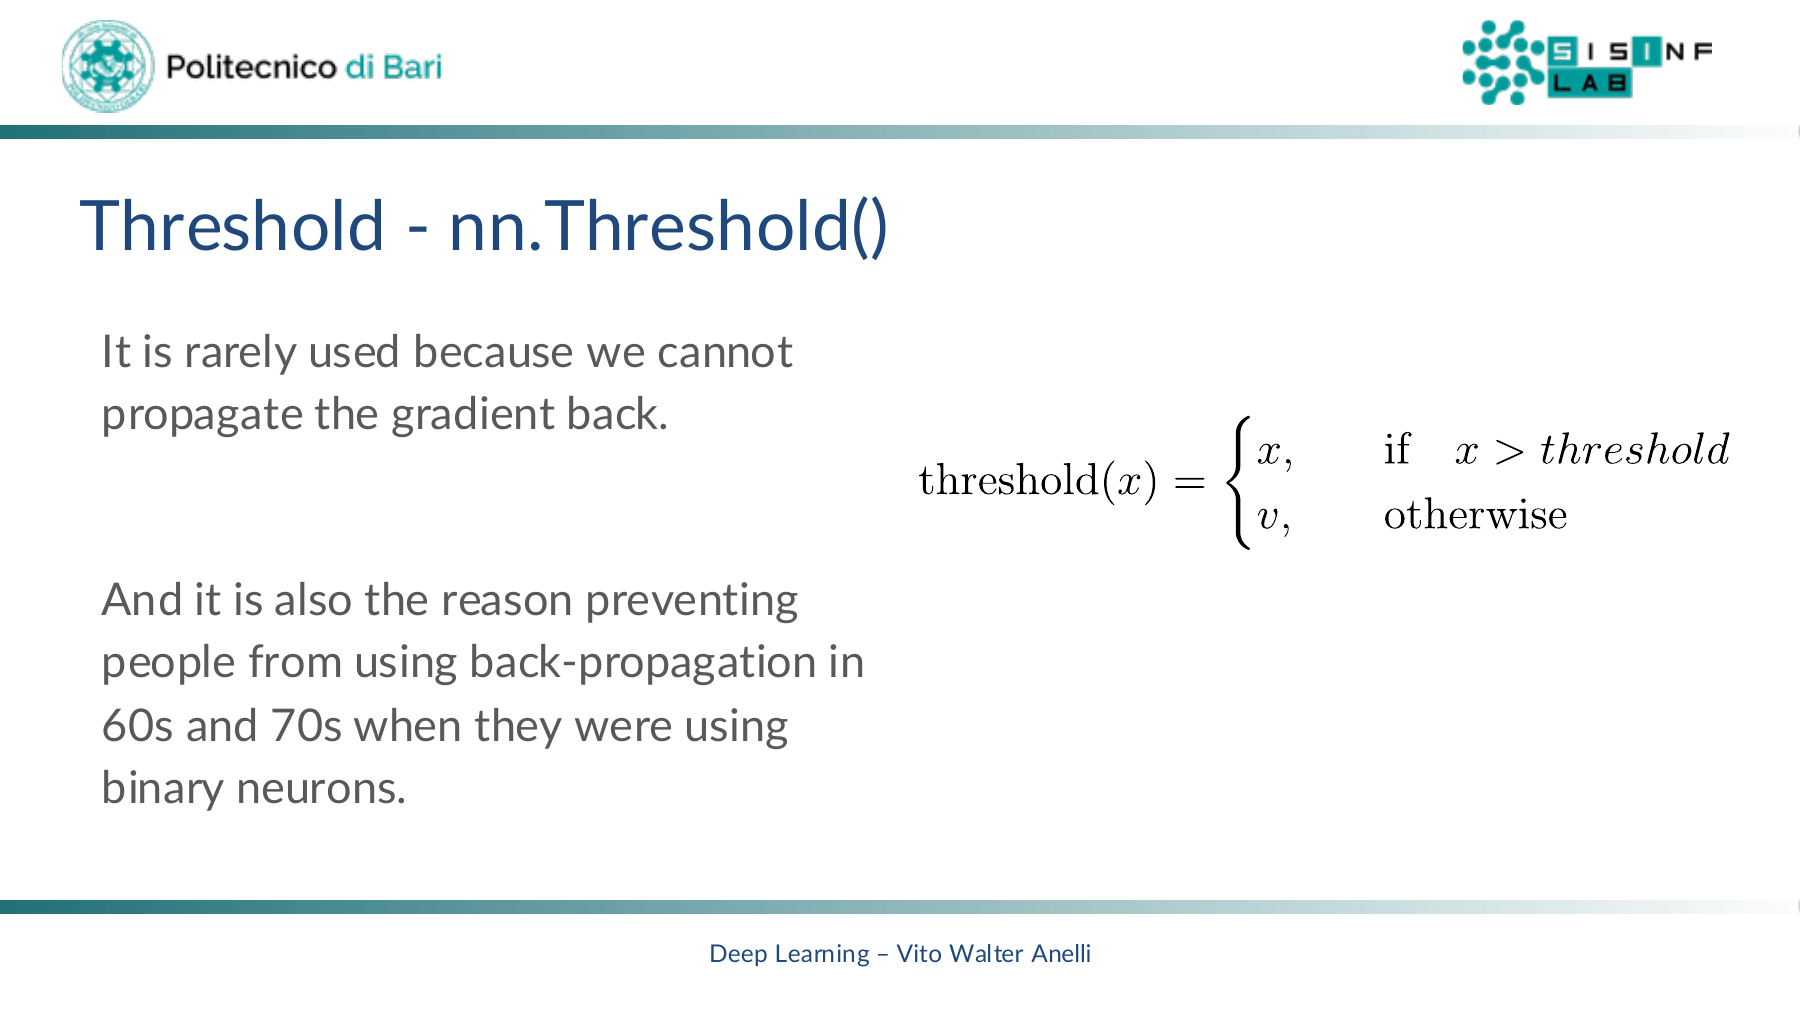
\includegraphics[width=0.72\linewidth]{figures/af03_threshold.png}
  \caption{Threshold (neurone binario): il gradiente è zero nella regione
           subthreshold, rendendo impossibile la retropropagazione per quei neuroni.
           È la ragione storica per cui la backpropagation non venne adottata
           negli anni '60--'70, quando si usavano neuroni binari.
           Attualmente non è utilizzata in reti moderne.}
  \label{fig:threshold}
\end{figure}

\subsection{Tanhshrink -- \texttt{nn.Tanhshrink()}}
\label{subsec:tanhshrink}

\begin{equation}
  \operatorname{Tanhshrink}(x) = x - \tanh(x).
\end{equation}

\begin{figure}[H]
  \centering
  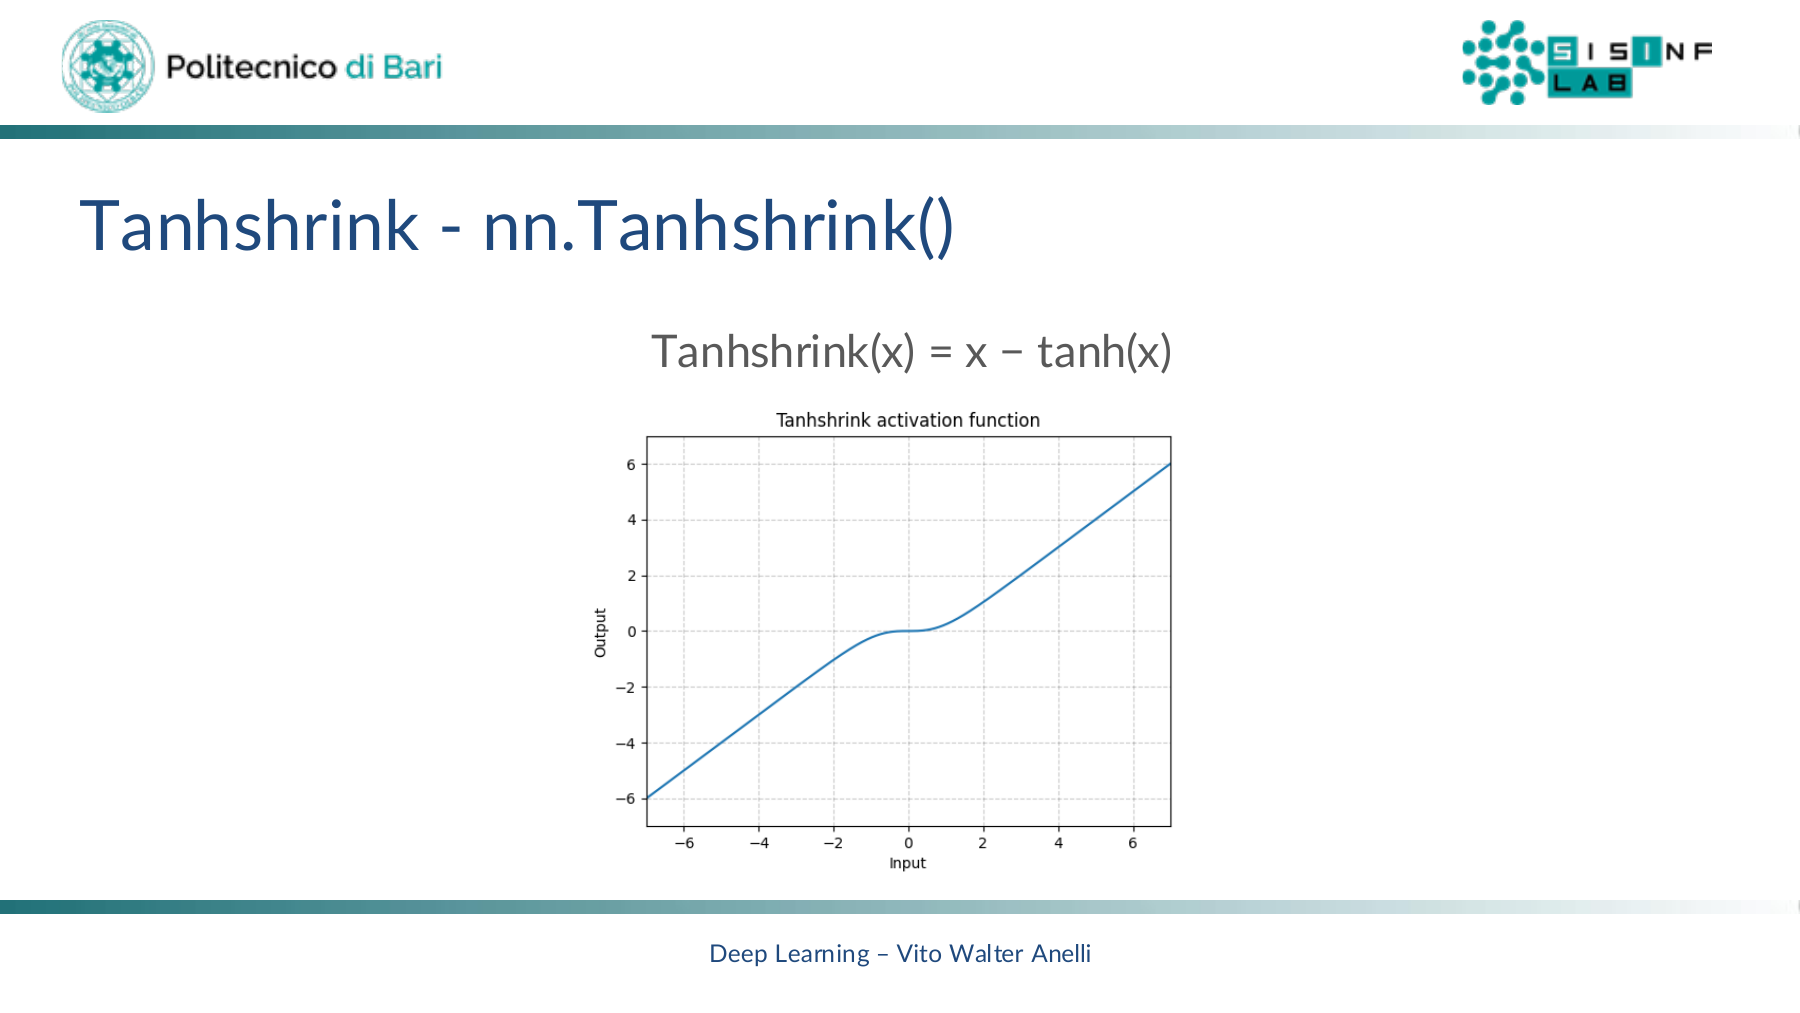
\includegraphics[width=0.72\linewidth]{figures/af03_tanhshrink.png}
  \caption{Tanhshrink: sottrae $\tanh(x)$ dall'input, producendo una funzione
           quasi lineare (con una lieve curvatura centrale). Usata in contesti
           di sparse coding per promuovere rappresentazioni sparse.}
  \label{fig:tanhshrink}
\end{figure}

\subsection{Softshrink -- \texttt{nn.Softshrink()}}
\label{subsec:softshrink}

\begin{equation}
  \operatorname{Softshrinkage}(x) =
  \begin{cases}
    x - \lambda, & \text{se } x > \lambda \\
    x + \lambda, & \text{se } x < -\lambda \\
    0,           & \text{altrimenti}
  \end{cases}
\end{equation}

\begin{figure}[H]
  \centering
  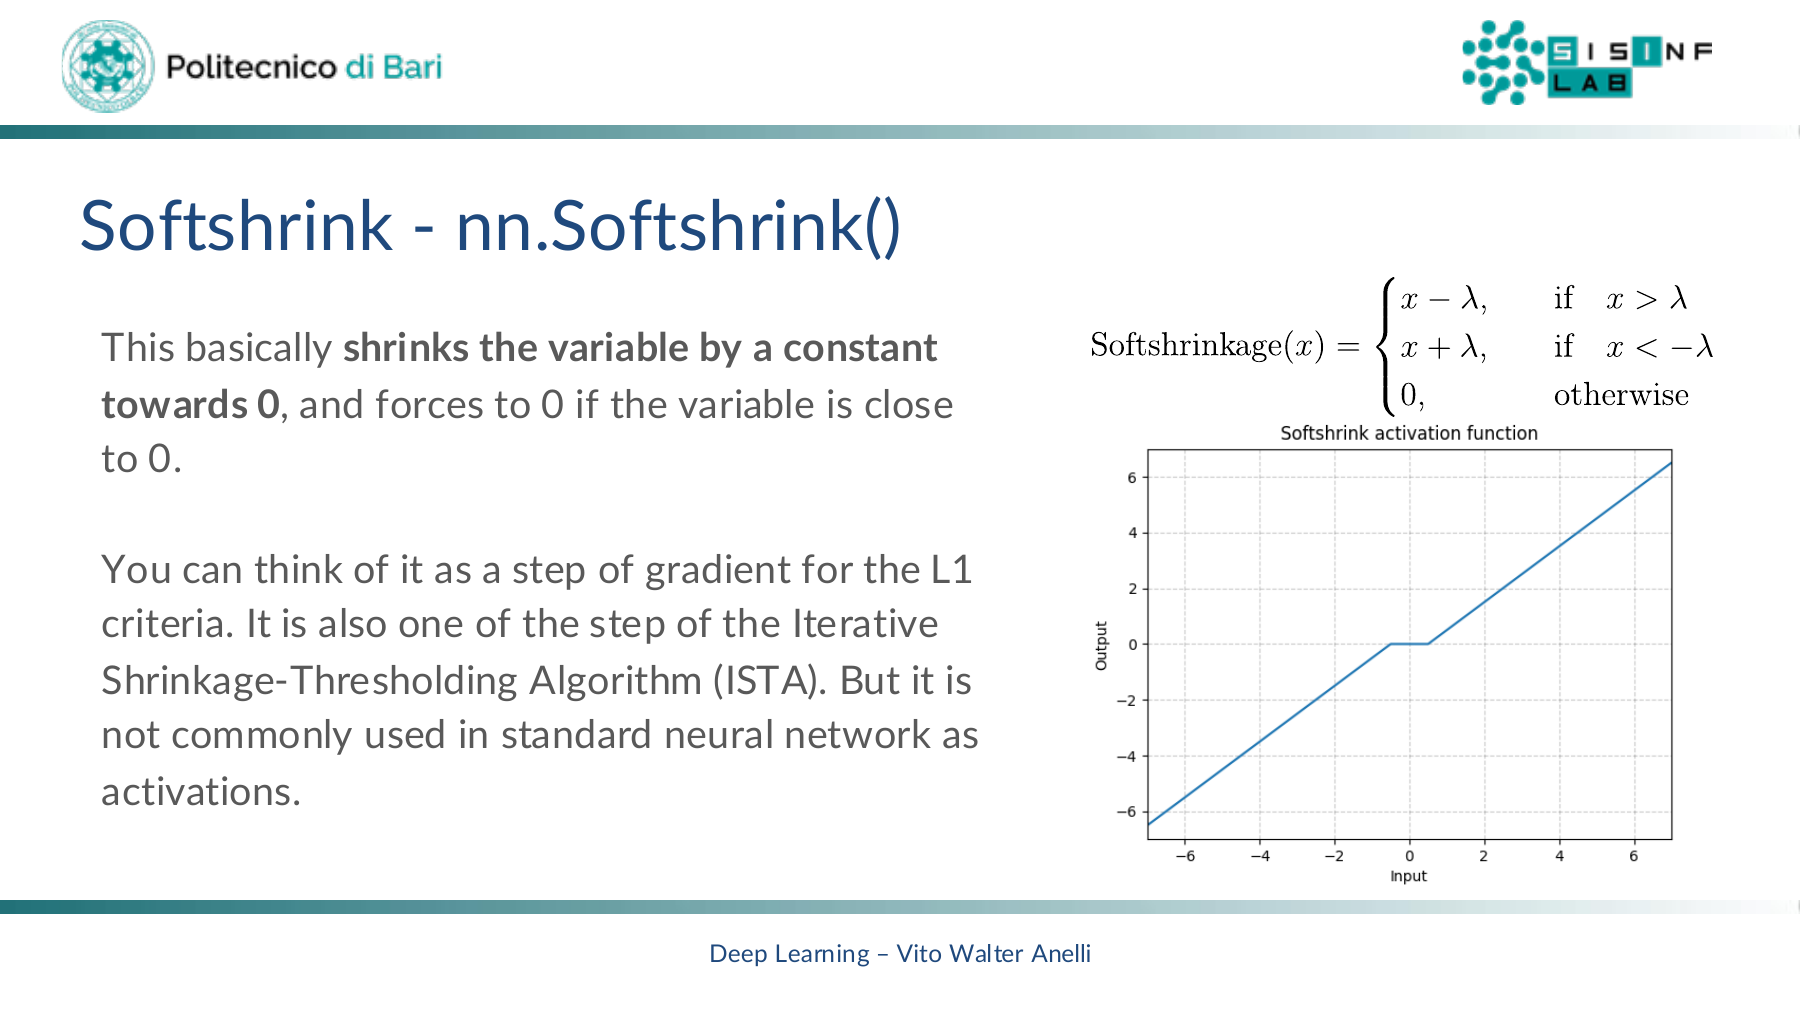
\includegraphics[width=0.85\linewidth]{figures/af03_softshrink.png}
  \caption{Softshrink: riduce il valore assoluto di $x$ di $\lambda$ verso zero,
           forzando a zero gli input nell'intervallo $[-\lambda, \lambda]$.
           Corrisponde a un passo del gradiente per la norma $L_1$ ed è
           uno step dell'algoritmo ISTA (\emph{Iterative Shrinkage-Thresholding}).
           Non è comunemente usata come attivazione nelle reti standard.}
  \label{fig:softshrink}
\end{figure}

\subsection{Hardshrink -- \texttt{nn.Hardshrink()}}
\label{subsec:hardshrink}

\begin{equation}
  \operatorname{Hardshrink}(x) =
  \begin{cases}
    x, & \text{se } x > \lambda \\
    x, & \text{se } x < -\lambda \\
    0, & \text{altrimenti}
  \end{cases}
\end{equation}

\begin{figure}[H]
  \centering
  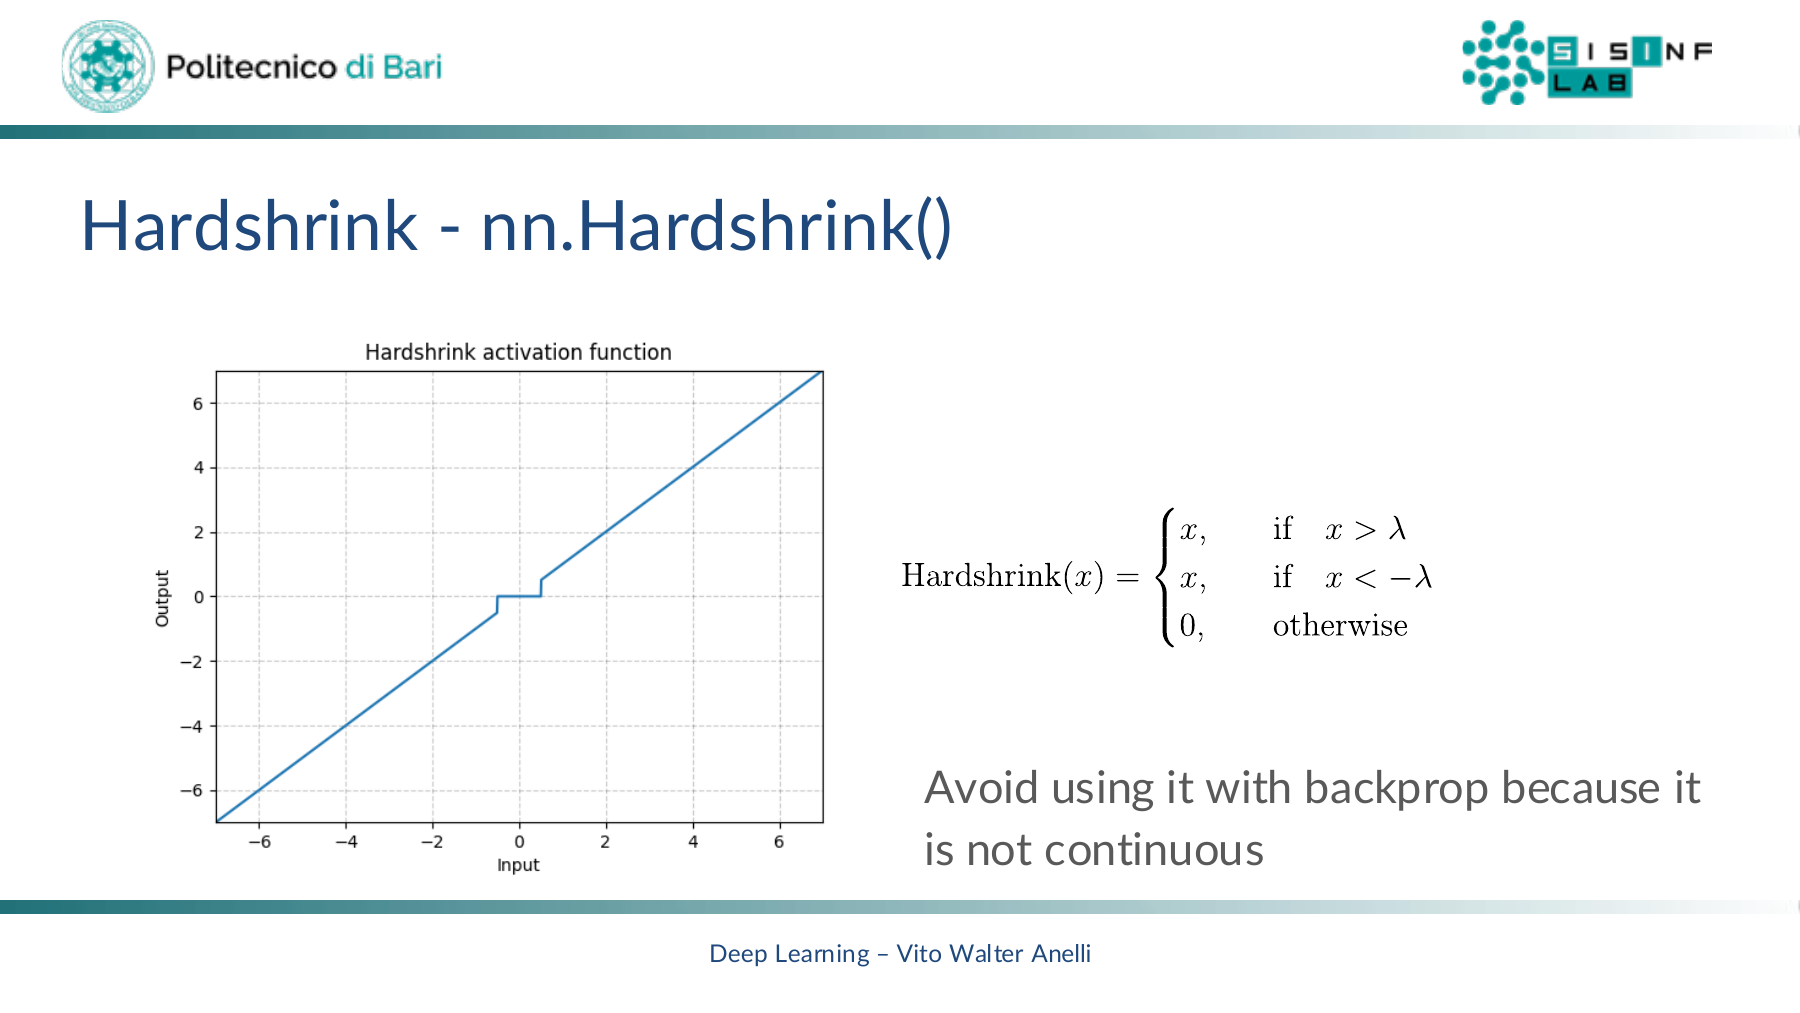
\includegraphics[width=0.85\linewidth]{figures/af03_hardshrink.png}
  \caption{Hardshrink: variante discontinua di Softshrink. La discontinuità in
           $x = \pm\lambda$ rende il gradiente non definito in quei punti, per
           cui \textbf{è sconsigliato l'uso con backpropagation}.
           Utilizzata in alcuni algoritmi di sparse coding fuori dal contesto
           delle reti neurali gradient-based.}
  \label{fig:hardshrink}
\end{figure}

%------------------------------------------------------------
\section{LogSigmoid -- \texttt{nn.LogSigmoid()}}
\label{sec:logsigmoid}

\begin{equation}
  \operatorname{LogSigmoid}(x) = \log\!\left(\frac{1}{1+\exp(-x)}\right).
\end{equation}

\begin{figure}[H]
  \centering
  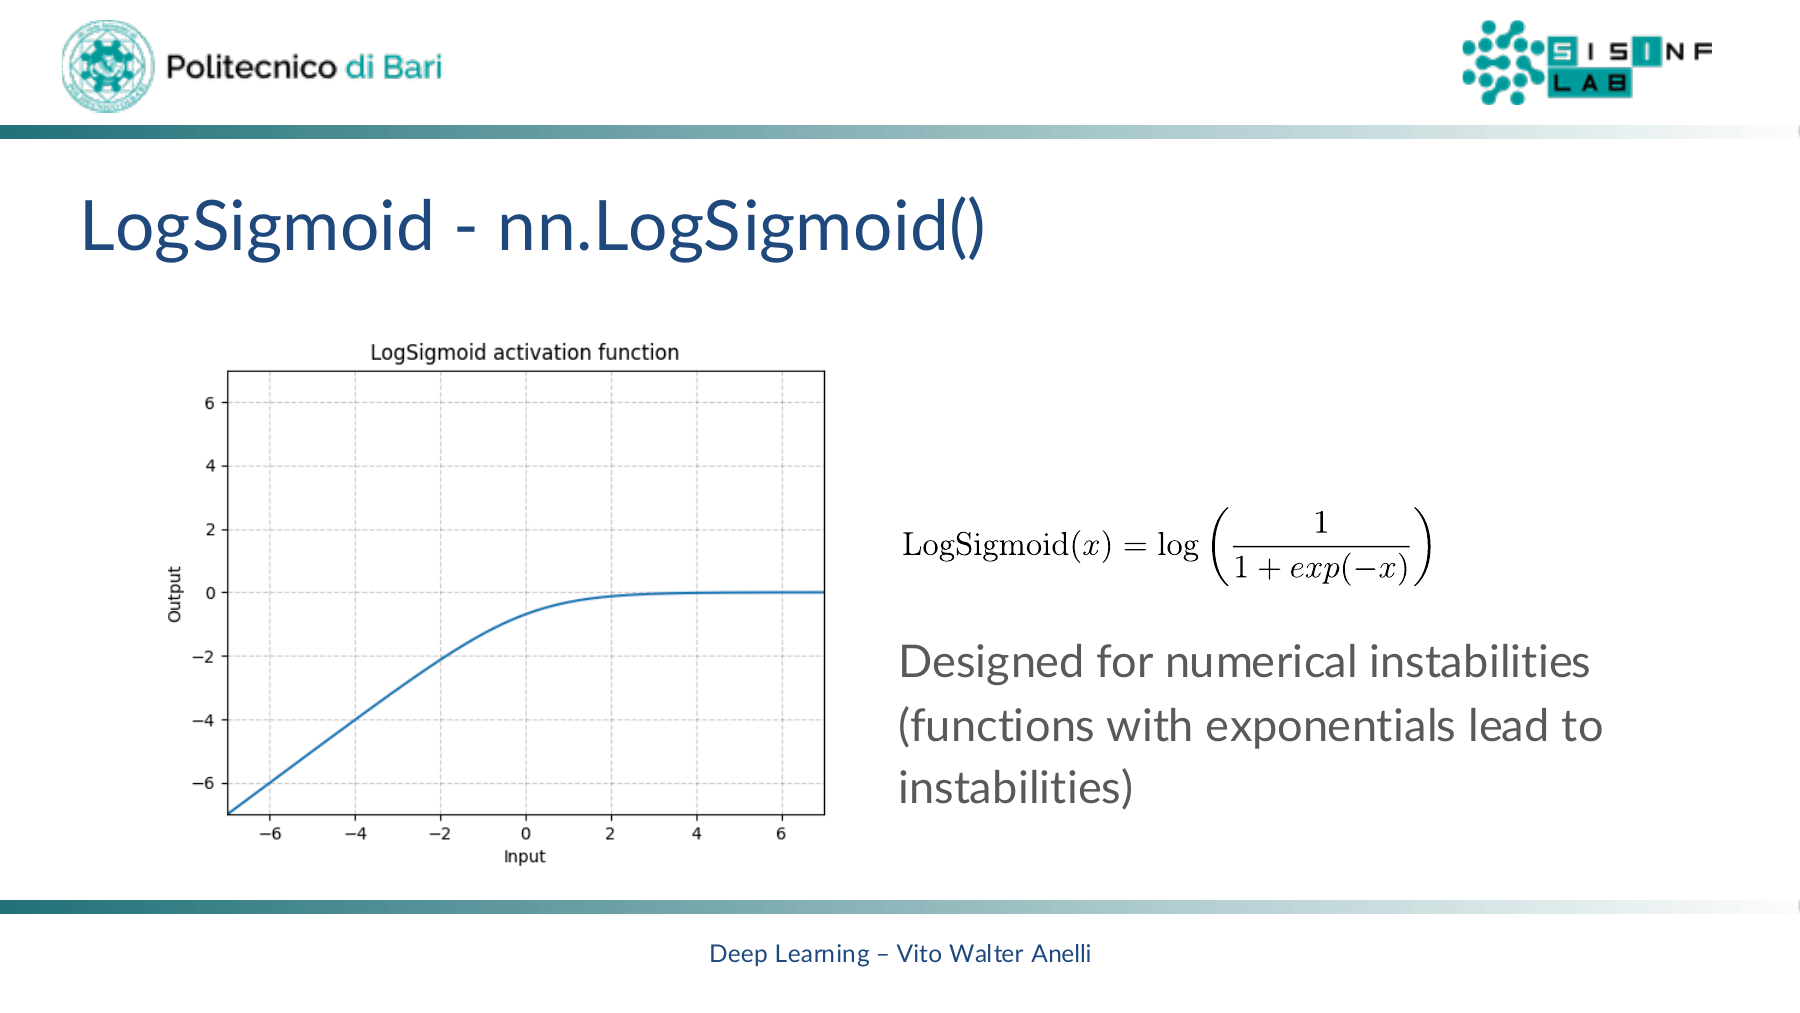
\includegraphics[width=0.85\linewidth]{figures/af03_logsigmoid.png}
  \caption{LogSigmoid: logaritmo della Sigmoid. Progettata per gestire le
           instabilità numeriche che emergono quando funzioni con esponenziali
           vengono composte (overflow/underflow). Usata prevalentemente nelle
           funzioni di costo, non come attivazione interna.}
  \label{fig:logsigmoid}
\end{figure}

%------------------------------------------------------------
\section{Funzioni Vettoriali: Softmin, Softmax, LogSoftmax}
\label{sec:softmax}

Le funzioni di questa sezione agiscono su \textbf{vettori interi}, trasformando
un vettore di scores in una distribuzione di probabilità. Non sono usate come
attivazioni interne, ma tipicamente nell'ultimo layer per compiti di
classificazione multiclasse.

\subsection{Softmin -- \texttt{nn.Softmin()}}
\label{subsec:softmin}

\begin{equation}
  \operatorname{Softmin}(x_i) = \frac{\exp(-x_i)}{\sum_j \exp(-x_j)}.
\end{equation}

\begin{figure}[H]
  \centering
  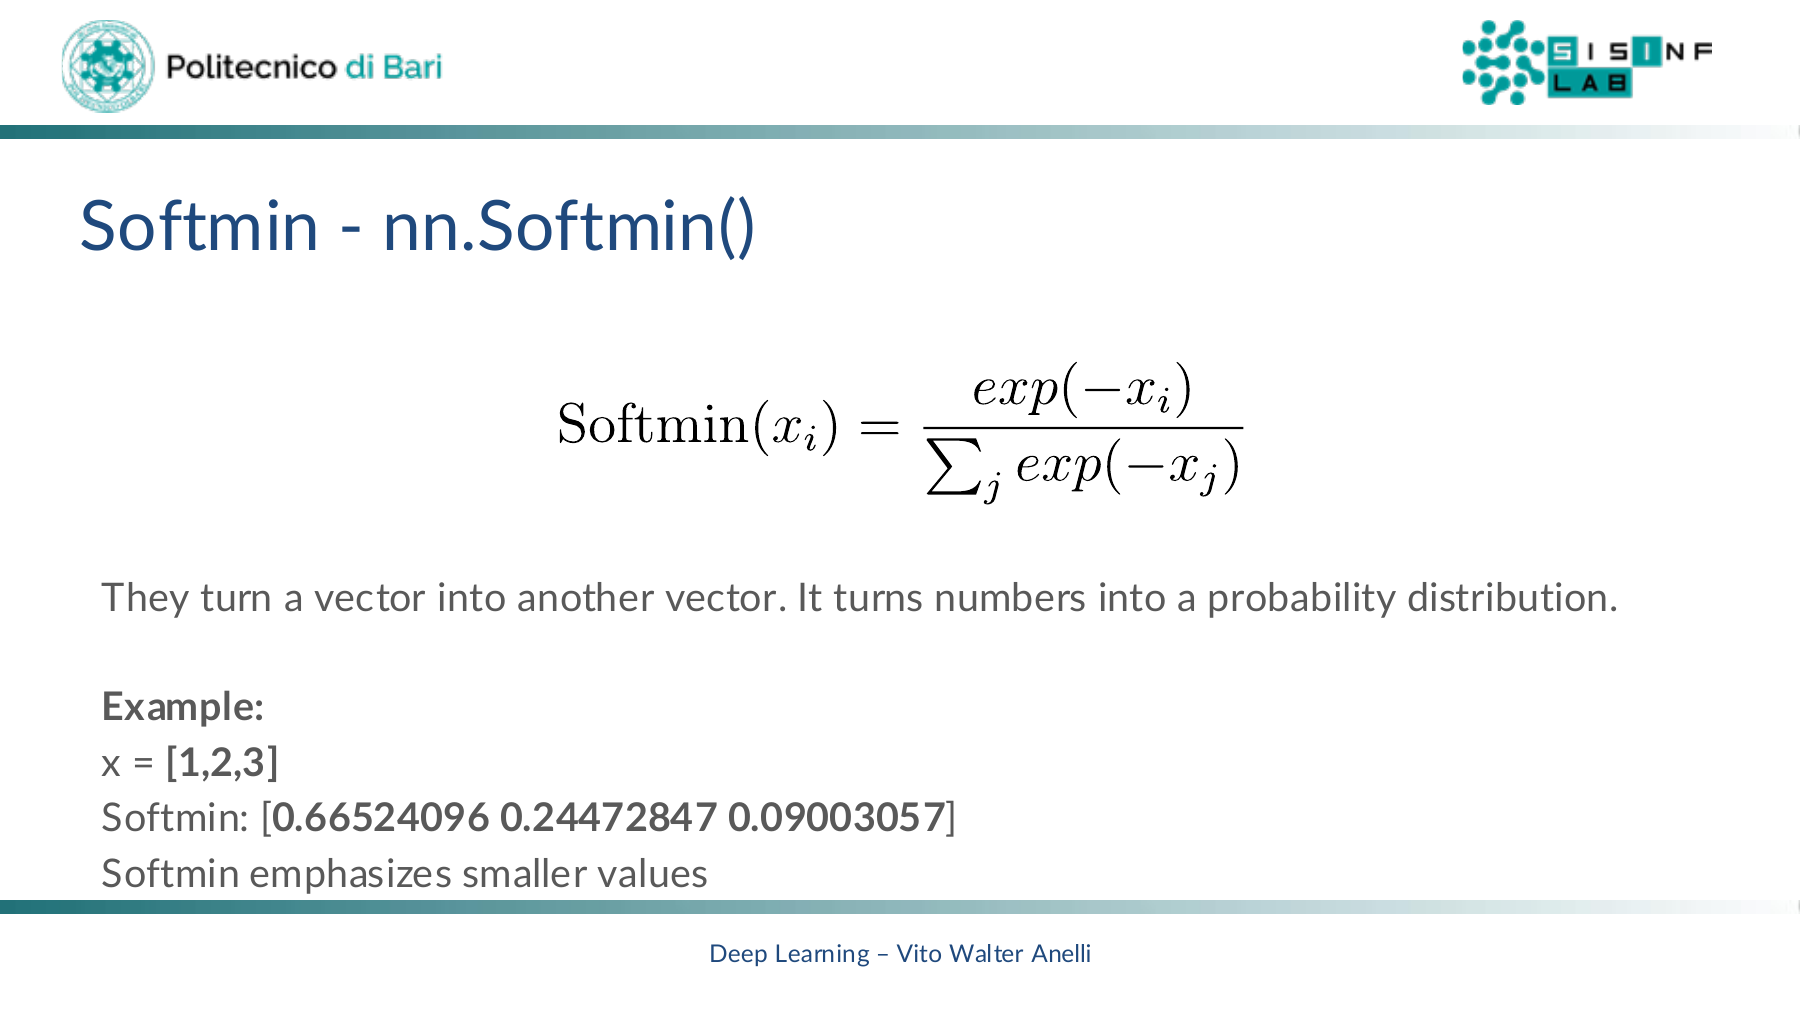
\includegraphics[width=0.72\linewidth]{figures/af03_softmin.png}
  \caption{Softmin: enfatizza i valori più \emph{piccoli} del vettore input.
           Per $x = [1,2,3]$ produce $[0{,}665,\, 0{,}245,\, 0{,}090]$:
           il valore più piccolo ($1$) riceve la probabilità maggiore.
           Raro in pratica; utile in contesti dove si vuole ``selezionare''
           il minimo in modo differenziabile.}
  \label{fig:softmin}
\end{figure}

\subsection{Soft(arg)max -- \texttt{nn.Softmax()}}
\label{subsec:softmax}

\begin{equation}
  \operatorname{Softmax}(x_i) = \frac{\exp(x_i)}{\sum_j \exp(x_j)}.
\end{equation}

\begin{figure}[H]
  \centering
  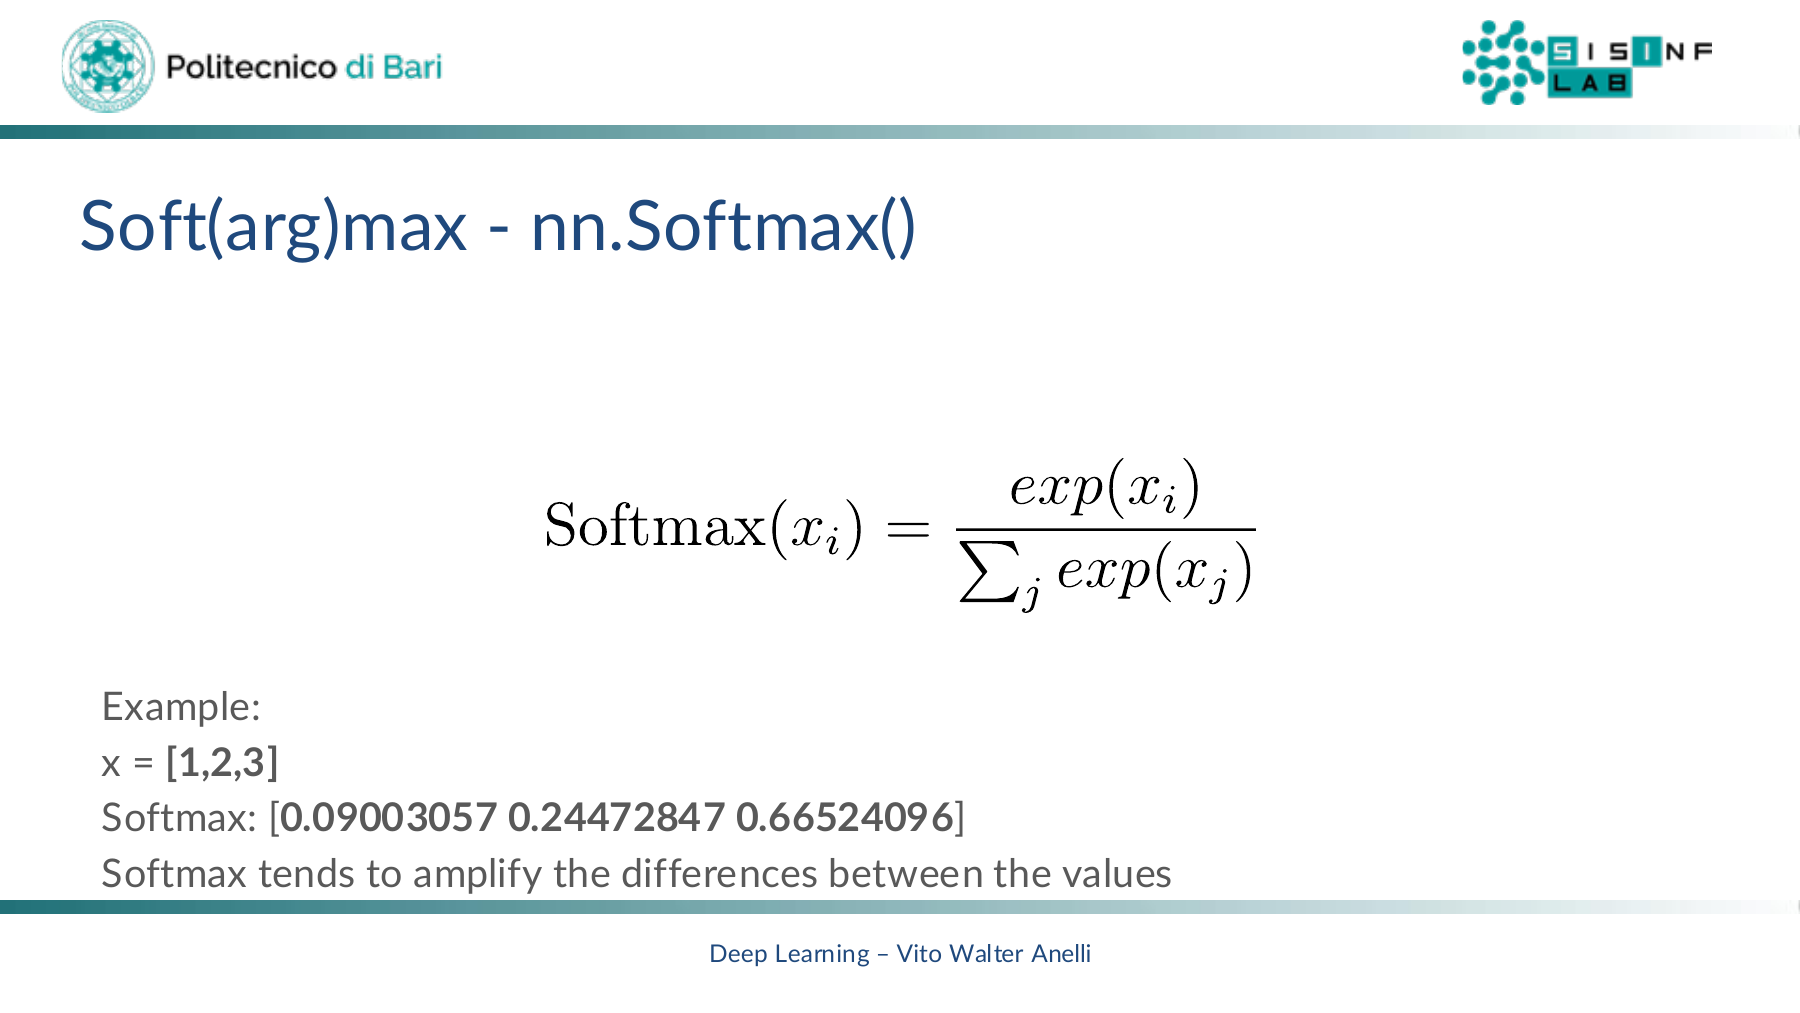
\includegraphics[width=0.72\linewidth]{figures/af03_softmax.png}
  \caption{Softmax: trasforma uno score vettoriale in una distribuzione di
           probabilità sommante a $1$. Enfatizza il valore più grande:
           per $x=[1,2,3]$ produce $[0{,}090,\, 0{,}245,\, 0{,}665]$.
           Amplifica le differenze tra i valori (\emph{winner-takes-all}).}
  \label{fig:softmax}
\end{figure}

\paragraph{Softmax come generalizzazione di Sigmoid.}
La Sigmoid è un caso speciale della Softmax per due classi.
Fissando $x_2 = 0$:

\begin{equation}
  z_1 = \frac{e^{x_1}}{e^{x_1} + e^{x_2}}
      \xrightarrow{x_2=0}
      \frac{e^{x_1}}{e^{x_1} + 1}
      = \frac{1}{1 + e^{-x_1}} = \sigma(x_1).
\end{equation}

\begin{figure}[H]
  \centering
  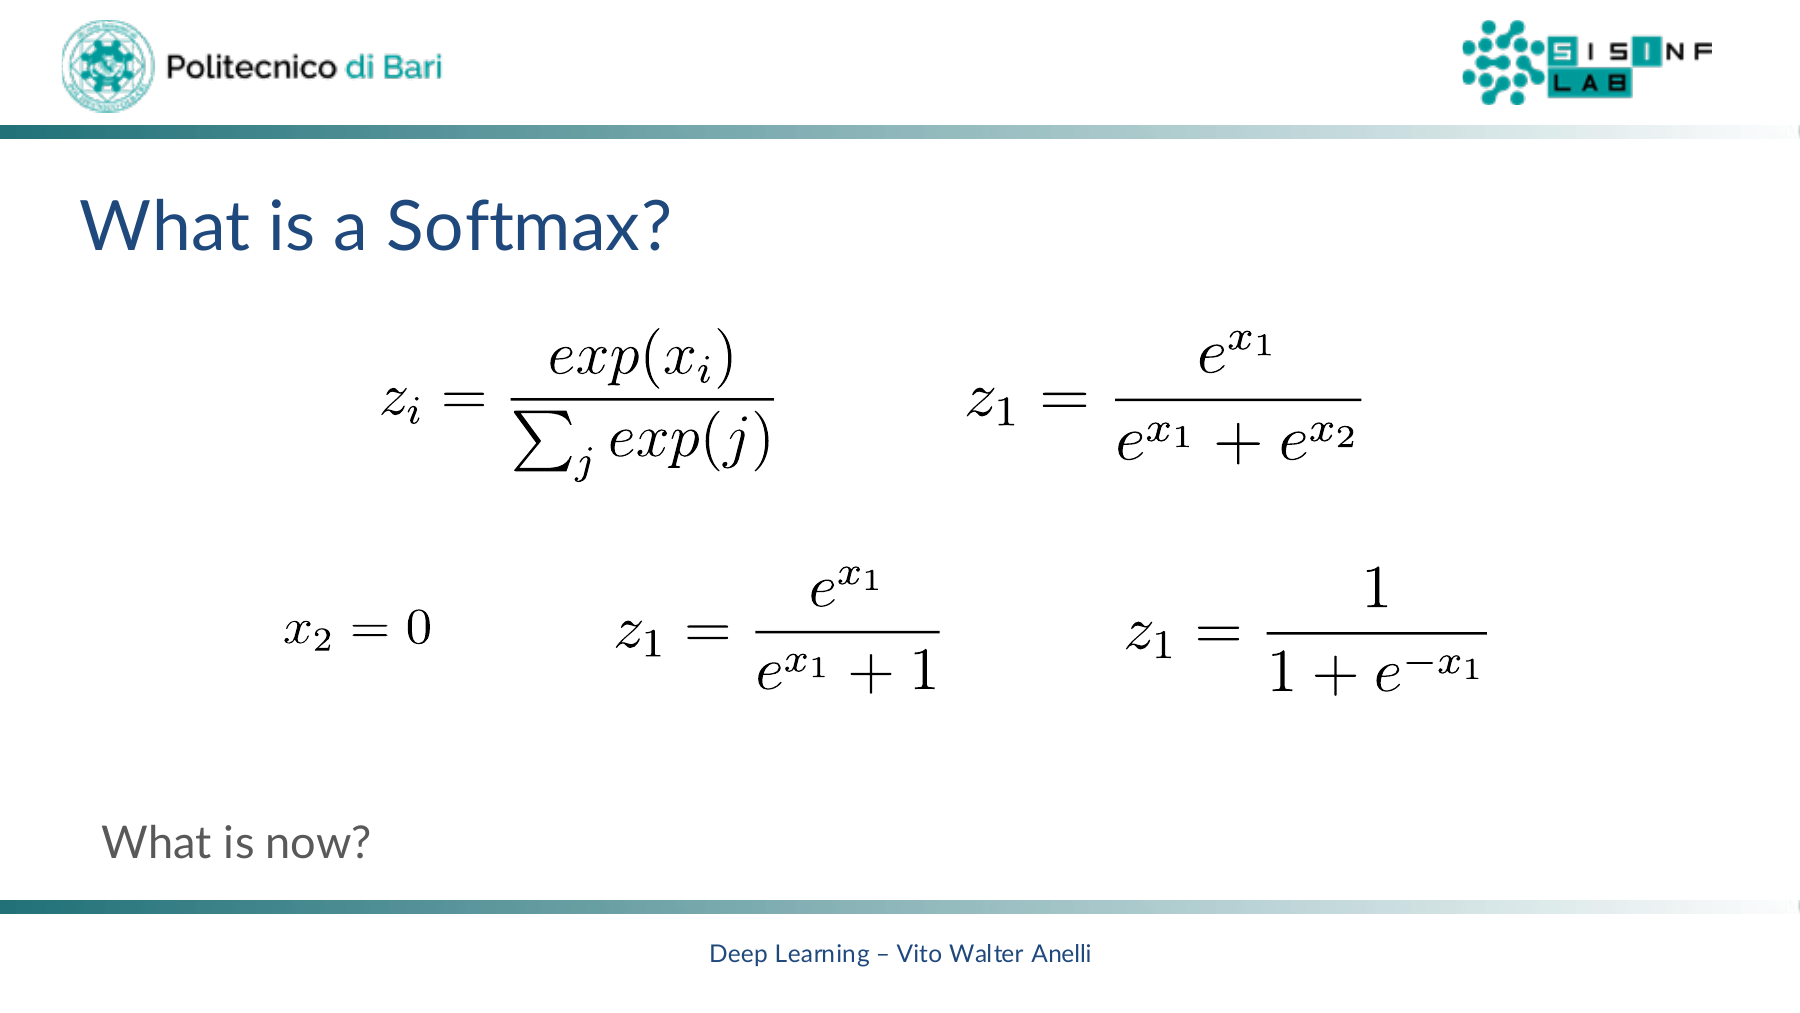
\includegraphics[width=0.72\linewidth]{figures/af03_softmax_relation_sigmoid.png}
  \caption{Derivazione della Sigmoid come caso speciale della Softmax a 2 classi.
           Questa relazione spiega perché la regressione logistica binaria
           (che usa Sigmoid) è un caso speciale della Softmax multiclasse.}
  \label{fig:softmax_relation_sigmoid}
\end{figure}

\subsection{LogSoft(arg)max -- \texttt{nn.LogSoftmax()}}
\label{subsec:logsoftmax}

\begin{equation}
  \operatorname{LogSoftmax}(x_i) = \log\!\left(\frac{\exp(x_i)}{\sum_j \exp(x_j)}\right).
\end{equation}

\begin{figure}[H]
  \centering
  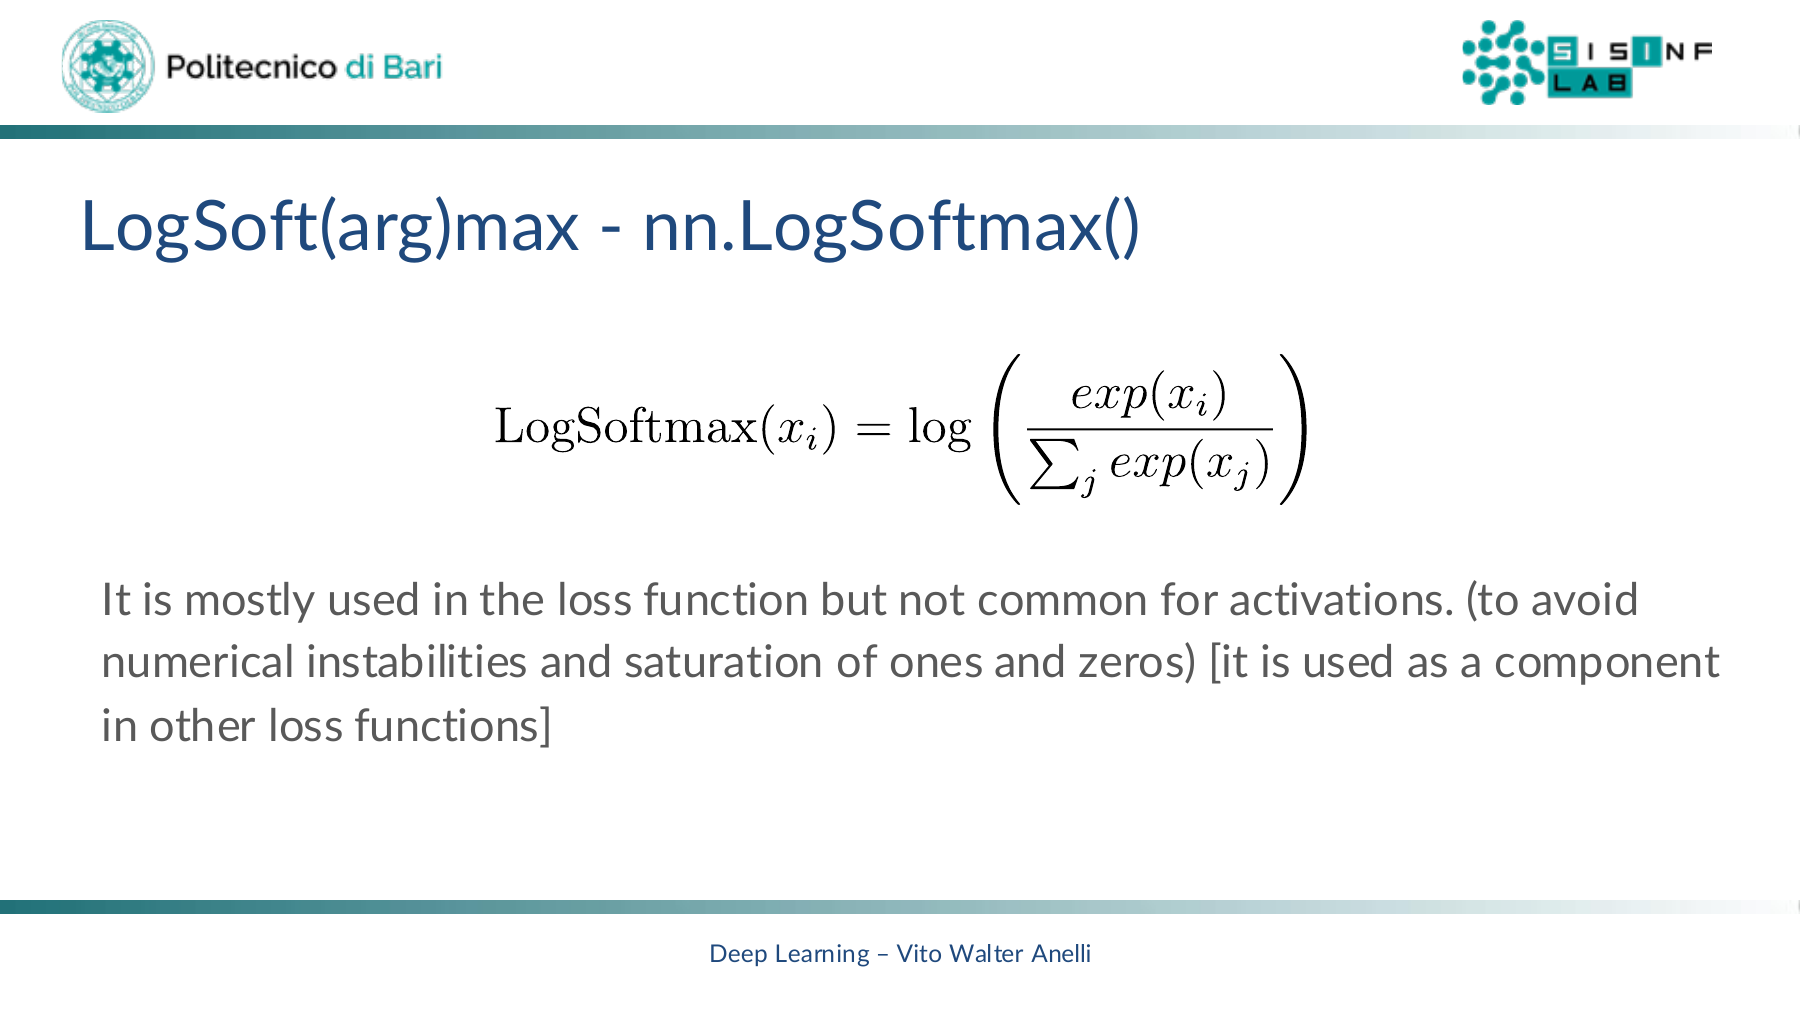
\includegraphics[width=0.72\linewidth]{figures/af03_logsoftmax.png}
  \caption{LogSoftmax: usato principalmente nelle funzioni di costo (es.\ in
           combinazione con \texttt{nn.NLLLoss}) per evitare instabilità
           numeriche (overflow/underflow per esponenziali grandi) e la
           saturazione di valori in $0$ e $1$. Non è comune come attivazione
           interna.}
  \label{fig:logsoftmax}
\end{figure}

%------------------------------------------------------------
\section{Softmax e Cross-Entropy Loss}
\label{sec:softmax-crossentropy}

Nell'ultimo layer di un classificatore multiclasse, la Softmax viene accoppiata
alla \textbf{Cross-Entropy Loss}:

\begin{equation}
  \mathcal{L}_{\mathrm{CE}} = -\sum_i q_i \log(p_i),
\end{equation}
dove $q_i \in \{0,1\}$ è la label one-hot e $p_i = \operatorname{Softmax}(x_i)$.
Per un vettore one-hot, la somma collassa a un solo termine:

\begin{equation}
  \mathcal{L}_{\mathrm{CE}} = -\log\bigl(\operatorname{Softmax}(x_{\mathrm{corr}})\bigr),
\end{equation}
ossia si \emph{massimizza la probabilità assegnata alla classe corretta}
(o equivalentemente si minimizza il suo logaritmo negativo).

\begin{figure}[H]
  \centering
  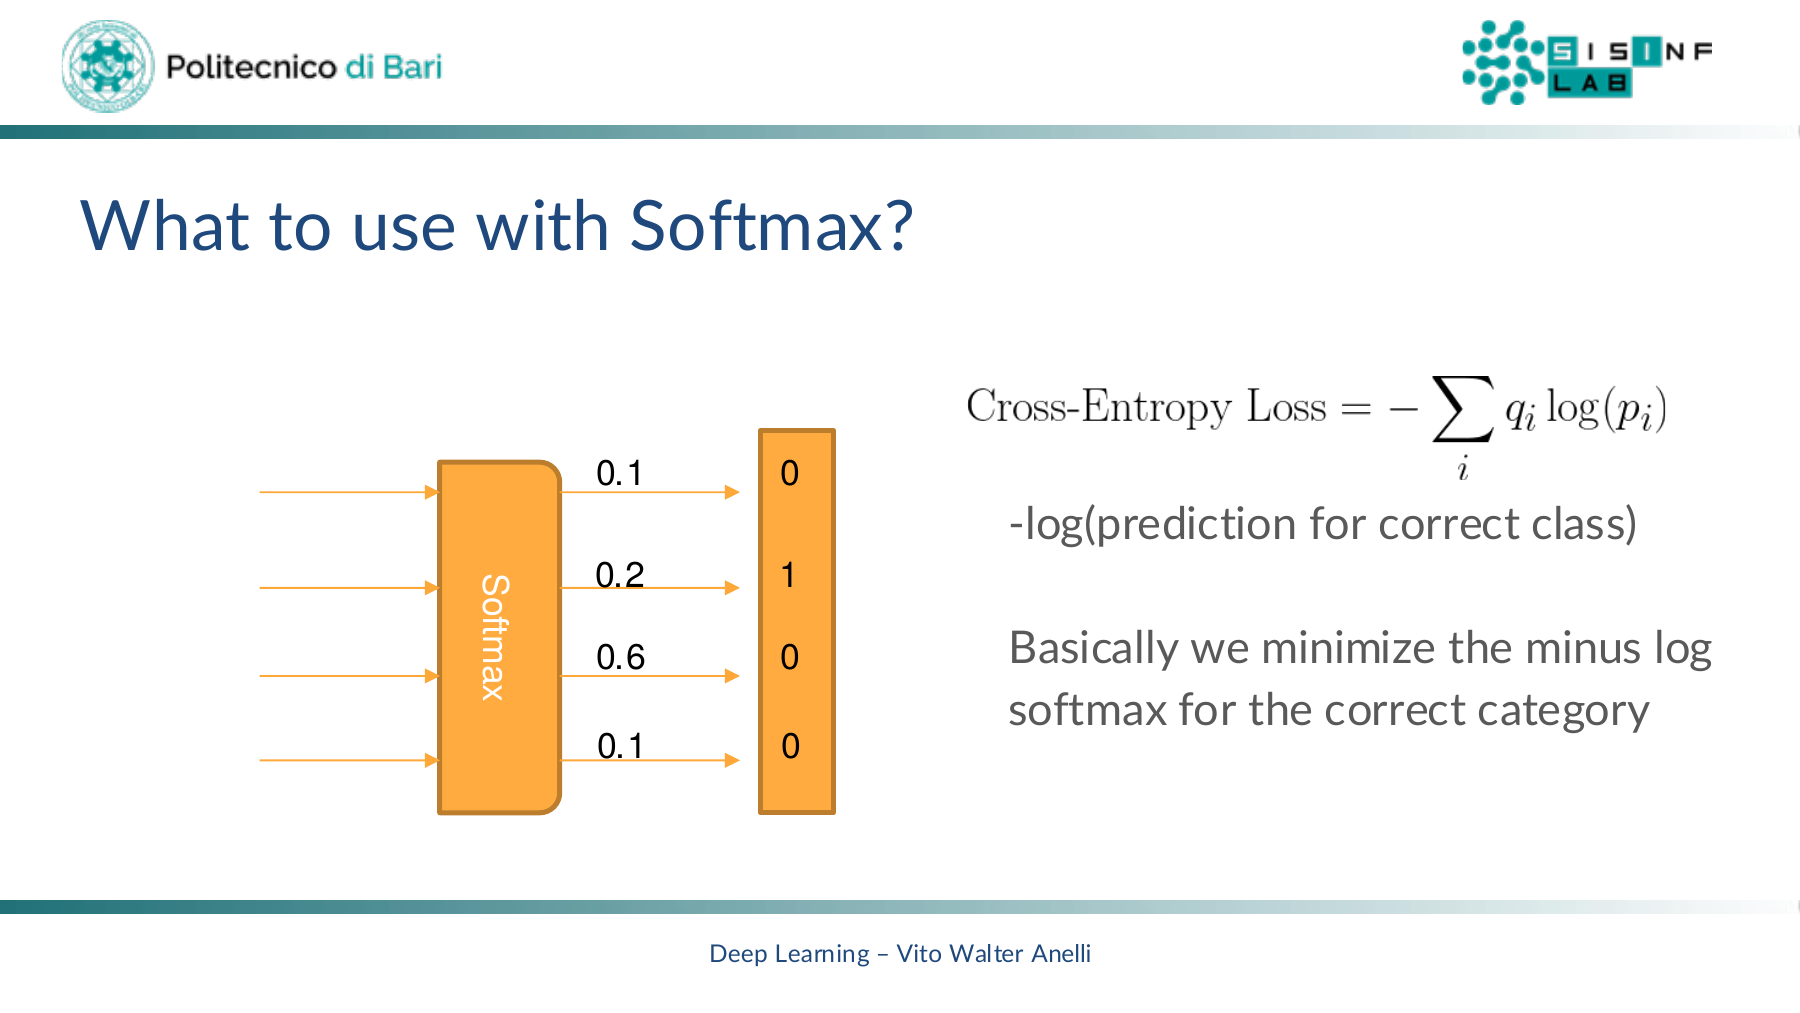
\includegraphics[width=0.82\linewidth]{figures/af03_softmax_crossentropy.png}
  \caption{Softmax + Cross-Entropy Loss: il layer Softmax produce una distribuzione
           $[0{,}1,\ 0{,}2,\ 0{,}6,\ 0{,}1]$ mentre il target one-hot seleziona
           la classe 2 ($[0,1,0,0]$). La loss è $-\log(0{,}2)$. In pratica
           si usa \texttt{nn.CrossEntropyLoss} in PyTorch che fonde
           \texttt{LogSoftmax} e \texttt{NLLLoss} per stabilità numerica.}
  \label{fig:softmax_crossentropy}
\end{figure}

In PyTorch è raccomandato usare \texttt{nn.CrossEntropyLoss} anziché
\texttt{nn.Softmax} + \texttt{nn.NLLLoss} separatamente, perché la
formulazione unificata implementa il log-sum-exp trick che evita overflow
numerici \citep{bishop2024}.

%------------------------------------------------------------
\section{Guida Pratica alla Scelta}
\label{sec:practical-guide}

La scelta della funzione di attivazione dipende dal task, dalla profondità
della rete e dai requisiti computazionali. Le linee guida di \citet{bishop2024}
e del corso NYU-DL possono essere sintetizzate nella Tabella~\ref{tab:activation_guide}.

\begin{table}[H]
  \centering
  \caption{Guida pratica alla scelta della funzione di attivazione.}
  \label{tab:activation_guide}
  \small
  \begin{tabularx}{\linewidth}{l l l X}
    \toprule
    \textbf{Funzione} & \textbf{Output range} & \textbf{Gradiente} & \textbf{Uso tipico} \\
    \midrule
    ReLU       & $[0, +\infty)$                  & Non sat.\ (pos.) & Default hidden layer \\
    Leaky ReLU & $(-\infty,+\infty)$              & Non saturante    & ReLU con dead neurons \\
    PReLU      & $(-\infty,+\infty)$              & Apprendibile     & Quando LReLU è insufficiente \\
    ELU        & $(-\alpha, +\infty)$             & Non saturante    & Hidden, mean $\approx 0$ \\
    SELU       & $(\approx{-1{,}76}, +\infty)$   & Self-norm.       & Reti senza BatchNorm \\
    GELU       & $\approx(-0{,}17, +\infty)$     & Non mon.         & Transformer (BERT, GPT) \\
    Sigmoid    & $(0, 1)$                         & Saturante        & Output prob.\ binaria, gate \\
    Tanh       & $(-1, 1)$                        & Saturante        & RNN, output centrato \\
    Softmax    & $(0,1)^C$, $\sum=1$              & Vettoriale       & Output multiclasse \\
    \bottomrule
  \end{tabularx}
\end{table}

\paragraph{Raccomandazioni operative.}
\begin{enumerate}
  \item \textbf{Punto di partenza}: usare \textbf{ReLU} per i layer nascosti
        di MLP e CNN; è semplice, efficiente e funziona bene nella maggior parte
        dei casi.
  \item \textbf{Dead neurons}: se si osservano molti neuroni inattivi (output
        sempre zero), passare a \textbf{Leaky ReLU} o \textbf{ELU}.
  \item \textbf{Reti senza BatchNorm}: considerare \textbf{SELU}, che fornisce
        self-normalization automatica.
  \item \textbf{Transformer}: preferire \textbf{GELU}, che è la scelta standard
        in BERT, GPT-2/3 e modelli derivati.
  \item \textbf{Output layer}: usare \textbf{Sigmoid} per classificazione binaria,
        \textbf{Softmax} per multiclasse, nessuna attivazione (o ReLU/Softplus)
        per regressione con output positivo.
  \item \textbf{Loss function}: abbinare sempre \texttt{nn.CrossEntropyLoss}
        alla Softmax (fuse internamente con \texttt{LogSoftmax}) per stabilità
        numerica.
\end{enumerate}

%------------------------------------------------------------
\section{Riepilogo}
\label{sec:summary-ch3}

\begin{center}
\small
\begin{tabularx}{\linewidth}{l l X}
  \toprule
  \textbf{Problema} & \textbf{Causa} & \textbf{Soluzione} \\
  \midrule
  Vanishing gradient  & Saturazione Sigmoid/Tanh  & ReLU, ELU, GELU \\
  Dead neurons        & ReLU $=0$ per input neg.  & LReLU, PReLU, ELU \\
  Output non centrato & ReLU $\geq 0$ sempre      & ELU, SELU, BatchNorm \\
  Instabilità num.    & Exp.\ overflow in Softmax & LogSoftmax, CrossEntropyLoss \\
  Parametri extra     & PReLU: $a$ apprendibile   & Beneficio: adattività \\
  Non monotonicità    & GELU ha un ``dip''         & Proprietà regolatrice \\
  \bottomrule
\end{tabularx}
\end{center}

Le funzioni di attivazione rappresentano uno degli assi portanti
dell'ingegneria delle reti neurali: la scelta sbagliata può precludere
l'apprendimento nei layer profondi (vanishing gradient), mentre la scelta
giusta velocizza la convergenza e migliora la generalizzazione.
Il consenso attuale nella letteratura è di usare ReLU o le sue varianti
non saturanti come default, riservando Sigmoid e Tanh ai casi in cui
la struttura del problema lo impone (output probabilistici, meccanismi
di gating, reti ricorrenti).

%============================================================
%  Capitolo 4 – Loss Functions
%============================================================
\chapter{Loss Functions}
\label{ch:loss-functions}

La \textbf{funzione di perdita} (loss function, o cost function) misura la discrepanza
tra la previsione della rete e il target desiderato. La scelta della loss è tanto
importante quanto quella dell'architettura: determina \textit{cosa} la rete impara
ad ottimizzare, e influenza il comportamento del gradiente durante il training.

In PyTorch tutte le loss sono implementate nel modulo \texttt{torch.nn} e seguono
una convenzione comune: accettano un input \texttt{x} (la predizione) e un target
\texttt{y}, e supportano l'argomento \texttt{reduction} (\texttt{'none'},
\texttt{'mean'}, \texttt{'sum'}) per controllare come le loss elementari vengono
aggregate sul batch \citep{bishop2024}.

%------------------------------------------------------------
\section{Loss per Regressione}
\label{sec:regression-losses}

\subsection{MSE Loss -- \texttt{nn.MSELoss()}}
\label{subsec:mse}

La \textbf{Mean Squared Error} (errore quadratico medio, norma L2 al quadrato)
è la loss di regressione più comune:

\begin{equation}
  l(x, y) = L = \{l_1, \ldots, l_N\}^\top, \qquad
  l_n = (x_n - y_n)^2,
\end{equation}

dove $N$ è la dimensione del batch. Con \texttt{reduction='none'} la loss viene
restituita come vettore; altrimenti:

\begin{equation}
  l(x, y) =
  \begin{cases}
    \operatorname{mean}(L), & \text{se reduction} = \texttt{'mean'} \\
    \operatorname{sum}(L),  & \text{se reduction} = \texttt{'sum'}
  \end{cases}
\end{equation}

La somma opera su tutti gli elementi e, con \texttt{'mean'}, divide per $n$.
Per evitare la divisione si usa \texttt{reduction='sum'}.

\paragraph{Pro e contro.}
MSE è differenziabile ovunque e penalizza fortemente gli errori grandi (il quadrato
amplifica gli outlier). In task di regressione con output continui è la scelta
predefinita, ma soffre di elevata sensibilità al rumore.

\subsection{L1 Loss -- \texttt{nn.L1Loss()}}
\label{subsec:l1}

La \textbf{Mean Absolute Error} (MAE) misura l'errore assoluto medio:

\begin{equation}
  l(x, y) = L = \{l_1, \ldots, l_N\}^\top, \qquad
  l_n = |x_n - y_n|.
\end{equation}

Supporta le stesse opzioni di riduzione di \texttt{nn.MSELoss()}.

\paragraph{Vantaggio rispetto a L2.}
L1 è più robusta agli outlier: gli errori non vengono elevati al quadrato, quindi
i punti rumorosi influenzano meno la loss totale. Il valore $y$ che minimizza la
distanza L1 è la \textbf{mediana} (anziché la media per L2), il che produce
predizioni meno sfocate in task come la super-risoluzione d'immagine.

\begin{quote}
\textit{L1 ha gradienti costanti: anche quando la loss si avvicina a zero,
il gradiente non si annulla, producendo immagini predette più nitide.}
\end{quote}

\paragraph{Limite.}
L1 \textbf{non è differenziabile in} $x=0$ (dove la funzione valore assoluto ha
un ``angolo''). Questo richiede attenzione nella gestione del gradiente
(cfr.\ \texttt{nn.Softshrink}). Per questo motivo è stata introdotta la
SmoothL1Loss.

\subsection{Smooth L1 Loss (Huber Loss) -- \texttt{nn.SmoothL1Loss()}}
\label{subsec:smooth-l1}

Combina L2 per errori piccoli e L1 per errori grandi, eliminando il problema
della non-differenziabilità in zero:

\begin{equation}
  \operatorname{loss}(x, y) = \frac{1}{n}\sum_i z_i, \qquad
  z_i =
  \begin{cases}
    0.5\,(x_i - y_i)^2,   & \text{se } |x_i - y_i| < 1 \\
    |x_i - y_i| - 0.5,    & \text{altrimenti}
  \end{cases}
\end{equation}

Nota anche come \textbf{Huber Loss} o \textbf{Elastic Network} quando usata come
funzione obiettivo. È stata resa popolare da Ross Girshick in Fast R-CNN.

\paragraph{Pro e contro.}
Meno sensibile agli outlier rispetto a MSE e smooth nel punto zero.
Usata frequentemente in \textbf{computer vision} (object detection) per
proteggere contro outlier nelle coordinate dei bounding box.
Il limite è la presenza del fattore di scala $0.5$ fisso nella regione quadratica.

\subsection{L1 vs.\ L2 in Computer Vision}
\label{subsec:l1-l2-cv}

In task di predizione d'immagine dove esistono molte possibili output $y$:

\begin{itemize}
  \item \textbf{MSE (L2)}: la previsione converge alla \textit{media} di tutte
        le possibili $y$. In visione artificiale questo produce immagini
        \textbf{sfocate} (blur), perché la media di immagini nitide con
        strutture leggermente diverse è un'immagine priva di dettagli.
  \item \textbf{L1}: la previsione converge alla \textit{mediana}, che non
        produce blur ma è difficile da definire in spazi multidimensionali.
\end{itemize}

\begin{figure}[H]
  \centering
  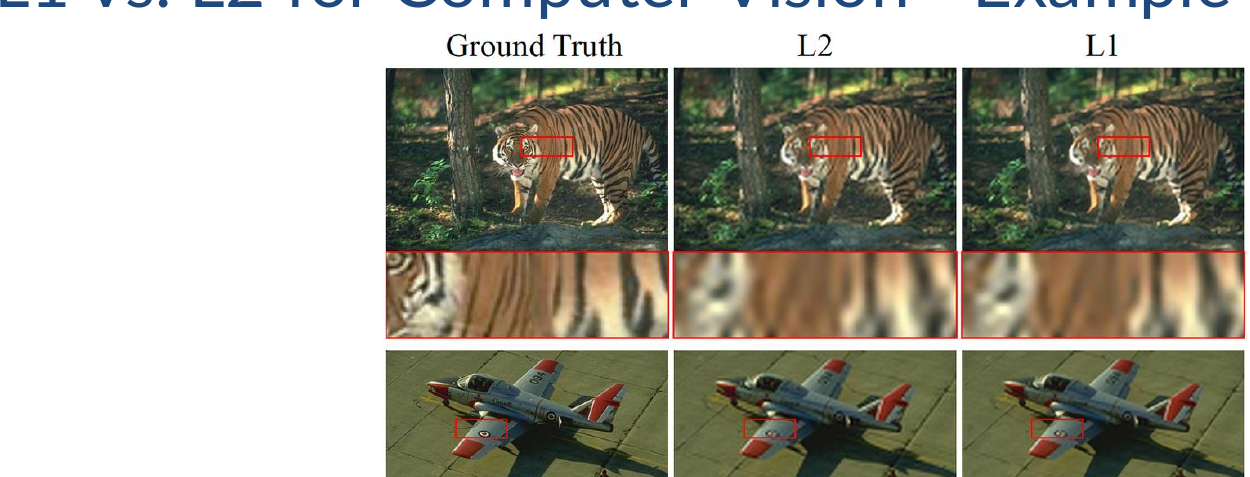
\includegraphics[width=0.82\linewidth]{figures/cf04_l1l2_cv_example.png}
  \caption{Confronto visivo tra Ground Truth, predizione con L2 (sfocata) e
           predizione con L1 (più nitida) su due esempi: una tigre e un aereo.
           Il dettaglio ingrandito mostra come L2 produca un'area blurred nel
           crop della tigre, mentre L1 preserva meglio le strutture.
           [Fonte: towardsdatascience.com/perceptual-losses-for-image-restoration]}
  \label{fig:l1l2_cv}
\end{figure}

%------------------------------------------------------------
\section{Loss per Classificazione}
\label{sec:classification-losses}

\subsection{NLL Loss -- \texttt{nn.NLLLoss()}}
\label{subsec:nll}

La \textbf{Negative Log Likelihood Loss} è usata per problemi di classificazione
con $C$ classi. Matematicamente, l'input dovrebbe essere una log-likelihood
(come l'output di \texttt{nn.LogSoftmax}), ma PyTorch non lo impone.

Loss non ridotta:
\begin{equation}
  l(x, y) = L = \{l_1, \ldots, l_N\}^\top, \qquad
  l_n = -w_{y_n}\, x_{n,\, y_n}, \qquad
  w_c = \operatorname{weight}[c] \cdot \mathbf{1}\{c \neq \texttt{ignore\_index}\}.
\end{equation}

Con riduzione:
\begin{equation}
  l(x,y) =
  \begin{cases}
    \displaystyle\sum_{n=1}^{N} \frac{1}{\sum_{n=1}^{N} w_{y_n}} l_n,
      & \text{se reduction} = \texttt{'mean'} \\[6pt]
    \displaystyle\sum_{n=1}^{N} l_n,
      & \text{se reduction} = \texttt{'sum'}
  \end{cases}
\end{equation}

L'argomento opzionale \textbf{weight} accetta un tensore 1D che assegna un peso
a ciascuna classe, utile per gestire dataset sbilanciati.

\subsection{Gestione dei Dataset Sbilanciati}
\label{subsec:imbalanced}

Quando la frequenza delle classi differisce notevolmente (es.\ influenza comune vs
cancro al polmone), si possono adottare due strategie:

\paragraph{Strategia 1 -- Pesi nella loss.}
Aumentare il peso \texttt{weight[c]} per le classi minoritarie in \texttt{NLLLoss}
o \texttt{CrossEntropyLoss}.

\paragraph{Strategia 2 -- Equalizzazione della frequenza (preferita).}
Invece di assegnare pesi, è meglio \textbf{equalizzare la frequenza nel training}
per sfruttare meglio i gradienti stocastici:
\begin{enumerate}
  \item Raccogliere i campioni di ogni classe in buffer separati.
  \item Generare ogni minibatch prendendo lo stesso numero di campioni da ciascun
        buffer.
  \item Quando il buffer della classe minoritaria si esaurisce, ricominciare
        dall'inizio (buffer circolare) finché tutti i campioni della classe
        maggioritaria sono stati usati.
\end{enumerate}

\textbf{Attenzione}: non ridurre artificialmente la classe maggioritaria scartando
campioni --- non sprecare dati. Se si equalizza la frequenza, il modello non
conosce più la frequenza reale delle classi. Per correggere questo, si eseguono
pochi epoch finali con la distribuzione reale delle classi, affinché il sistema
adatti i bias dell'output layer.

\subsection{Cross-Entropy Loss -- \texttt{nn.CrossEntropyLoss()}}
\label{subsec:cross-entropy}

Combina \texttt{nn.LogSoftmax} e \texttt{nn.NLLLoss} in un'unica classe,
massimizzando lo score della classe corretta:

\begin{equation}
  \operatorname{loss}(x, c) =
  -\log\!\left(\frac{\exp(x[c])}{\sum_j \exp(x[j])}\right)
  = -x[c] + \log\!\left(\sum_j \exp(x[j])\right).
\end{equation}

Con peso per classe $w[c]$:
\begin{equation}
  \operatorname{loss}(x, c) = w[c]\!\left(-x[c] + \log\!\left(\sum_j \exp(x[j])\right)\right).
\end{equation}

\paragraph{Perché unire LogSoftmax e NLLLoss?}
Quando il valore dopo Softmax è vicino a $0$ o $1$, il suo logaritmo tende a
$-\infty$ e la derivata del $\log$ vicino a $0$ tende a $+\infty$, causando
instabilità numerica durante la retropropagazione. Unendo le due operazioni,
i gradienti vengono saturati a valori ragionevoli tramite il \textbf{log-sum-exp trick}.

\paragraph{Interpretazione probabilistica: KL Divergence.}
La Cross-Entropy ha una lettura information-theoretic: misura la
\textbf{divergenza di Kullback-Leibler} tra la distribuzione predetta $q$ e
quella target $p$:

\begin{align}
  H(p, q) &= H(p) + \mathcal{D}_{KL}(p \,\|\, q) \\
  H(p, q) &= -\sum_i p(x_i)\log q(x_i) \qquad \text{(cross-entropy)} \\
  H(p)    &= -\sum_i p(x_i)\log p(x_i) \qquad \text{(entropia)} \\
  \mathcal{D}_{KL}(p\|q) &= \sum_i p(x_i)\log\frac{p(x_i)}{q(x_i)} \quad \text{(KL divergence)}
\end{align}

Nel caso classificazione, $p$ è il vettore one-hot (0 sulle classi errate, 1 sulla
corretta) e $q$ è il vettore Softmax delle predizioni. Minimizzare la Cross-Entropy
equivale a minimizzare la KL Divergence tra predizioni e target.

\subsection{Binary Cross Entropy -- \texttt{nn.BCELoss()}}
\label{subsec:bce}

Caso speciale della Cross-Entropy per \textbf{due classi}:

\begin{equation}
  l(x, y) = L = \{l_1, \ldots, l_N\}^\top, \qquad
  l_n = -w_n\bigl[y_n \log x_n + (1-y_n)\log(1-x_n)\bigr].
\end{equation}

Usata tipicamente per misurare l'errore di ricostruzione in un auto-encoder.
\textbf{Attenzione}: la formula assume che $x$ e $y$ siano probabilità, quindi
strettamente in $(0, 1)$.

\subsection{BCE with Logits -- \texttt{nn.BCEWithLogitsLoss()}}
\label{subsec:bce-logits}

Versione numericamente più stabile di BCELoss: accetta score grezzi (logit) non
normalizzati e applica internamente la Sigmoid prima del log:

\begin{equation}
  l_n = -w_n\bigl[y_n \log\sigma(x_n) + (1-y_n)\log(1-\sigma(x_n))\bigr].
\end{equation}

Non assume che $x \in (0,1)$ e combina Sigmoid + BCE in un'unica operazione
numericamente stabile. \textbf{È preferita a \texttt{nn.BCELoss}} nelle reti con
output layer lineare.

\subsection{NLL Loss Adattiva -- \texttt{nn.AdaptiveLogSoftmaxWithLoss()}}
\label{subsec:adaptive}

Approssimazione efficiente di Softmax per un numero molto elevato di classi
(nell'ordine dei milioni). Implementa il metodo descritto in
\textit{Efficient softmax approximation for GPUs} (Grave et al., 2017), che
raggruppa le classi per frequenza e usa head di dimensioni diverse per classi
rare vs frequenti.

\subsection{KL Divergence Loss -- \texttt{nn.KLDivLoss()}}
\label{subsec:kldiv}

\begin{equation}
  l(x, y) = L = \{l_1, \ldots, l_N\}^\top, \qquad
  l_n = y_n(\log y_n - \log x_n).
\end{equation}

Utile quando il target è una distribuzione one-hot. Assume che $x$ e $y$ siano
probabilità. \textbf{Svantaggio}: non è integrata con una Softmax o LogSoftmax,
quindi può soffrire di instabilità numerica. Per questo motivo si preferisce
\texttt{nn.CrossEntropyLoss} nella maggior parte dei casi.

%------------------------------------------------------------
\section{Loss Basate su Margine}
\label{sec:margin-losses}

Le \textbf{margin losses} sono una categoria importante di loss functions: invece
di misurare la distanza assoluta tra predizione e target, richiedono che la
predizione corretta superi quella errata di almeno un certo margine.

\subsection{Hinge Embedding Loss -- \texttt{nn.HingeEmbeddingLoss()}}
\label{subsec:hinge-embedding}

Usata in apprendimento semi-supervisionato per misurare la similarità/dissimilarità
tra coppie di input:

\begin{equation}
  l_n =
  \begin{cases}
    x_n,                        & y_n = 1  \\
    \max\{0,\, \delta - x_n\},  & y_n = -1
  \end{cases}
\end{equation}

La variabile $y$ indica se la coppia $(x)$ è simile ($+1$) o dissimile ($-1$).
Con la hinge loss, lo score è positivo se $y=1$ e viene penalizzato se $y=-1$
ma non supera il margine $\delta$.
Di solito si usa con la distanza L1 a coppie come $x$.

\subsection{Margin Ranking Loss -- \texttt{nn.MarginRankingLoss()}}
\label{subsec:margin-ranking}

\begin{equation}
  L(x, y) = \max\bigl(-y \cdot (x_1 - x_2) + \operatorname{margin},\; 0\bigr).
\end{equation}

Richiede che un input sia maggiore dell'altro di almeno \texttt{margin}:
\begin{itemize}
  \item $x_1, x_2$: score assegnati dalla rete a due item (positivo e negativo).
  \item $y = +1$: si vuole $x_1 > x_2$ (item positivo deve avere score maggiore).
  \item $y = -1$: si vuole $x_2 > x_1$ (flip del confronto).
  \item \texttt{margin}: soglia minima della differenza desiderata tra gli score.
\end{itemize}

Se $y \cdot (x_1 - x_2) > \operatorname{margin}$, il costo è $0$; altrimenti
cresce linearmente. In classificazione, $x_1$ è lo score della risposta corretta
e $x_2$ è lo score più alto tra le risposte errate nel minibatch.
Nei modelli energy-based (EBM), questa loss abbassa l'energia della risposta
corretta $x_1$ e alza quella della risposta errata $x_2$.

\subsection{Triplet Margin Loss -- \texttt{nn.TripletMarginLoss()}}
\label{subsec:triplet}

\begin{equation}
  L(a, p, n) = \max\bigl\{d(a_i, p_i) - d(a_i, n_i) + \operatorname{margin},\; 0\bigr\},
\end{equation}

dove $a$ è l'anchor, $p$ è il campione positivo (stessa classe), $n$ è quello
negativo (classe diversa) e $d(\cdot, \cdot)$ è una metrica di distanza.

Usata per misurare similarità relativa tra campioni:
\begin{itemize}
  \item Due immagini della stessa categoria passate a una CNN devono produrre
        vettori \textbf{vicini}.
  \item Due immagini di categorie diverse devono produrre vettori
        \textbf{lontani}.
\end{itemize}

La loss spinge la distanza della coppia positiva verso $0$ e quella della coppia
negativa oltre il margine. Ciò che conta è che la distanza della coppia buona sia
\textit{minore} di quella della coppia cattiva, non i valori assoluti.

\subsection{Soft Margin Loss -- \texttt{nn.SoftMarginLoss()}}
\label{subsec:soft-margin}

\begin{equation}
  L(x, y) = \sum_i \frac{\log\bigl(1 + \exp(-y[i] \cdot x[i])\bigr)}{n.\mathrm{nelement}()}.
\end{equation}

Versione \textbf{soft} (continua) della margin loss: ottimizza una perdita
logistica per classificazione a due classi con target $y \in \{-1, +1\}$.
Vuole che $\exp(-y[i] \cdot x[i])$ per la risposta corretta sia più piccolo che
per le altre: avvicina i valori positivi di $y[i] \cdot x[i]$ e allontana quelli
negativi, ma con un effetto esponenzialmente decrescente (a differenza di un hard
margin).

\subsection{Multi-Class Hinge Loss -- \texttt{nn.MultiLabelMarginLoss()}}
\label{subsec:multilabel-margin}

\begin{equation}
  L(x, y) = \sum_{ij} \frac{\max\bigl(0,\; 1 - (x[y[j]] - x[i])\bigr)}{x.\mathrm{size}(0)}.
\end{equation}

Estende la hinge loss al caso multiclasse, permettendo a diversi input di avere
quantità variabili di target. Somma la hinge loss su tutte le categorie target.
Nei modelli EBM, abbassa l'energia delle categorie desiderate e alza quella delle
non-desiderate.

%------------------------------------------------------------
\section{Loss per Embedding: Cosine Embedding Loss}
\label{sec:cosine-embedding}

\subsection{Formulazione}
\label{subsec:cosine-formula}

\texttt{nn.CosineEmbeddingLoss()} misura se due input sono simili o dissimili
usando la \textbf{distanza coseno}:

\begin{equation}
  l_n =
  \begin{cases}
    1 - \cos(x_1, x_2),                      & y = 1  \\
    \max\{0,\; \cos(x_1, x_2) - \operatorname{margin}\}, & y = -1
  \end{cases}
\end{equation}

Tipicamente usata per apprendere embedding non lineari o in apprendimento
semi-supervisionato.

\begin{figure}[H]
  \centering
  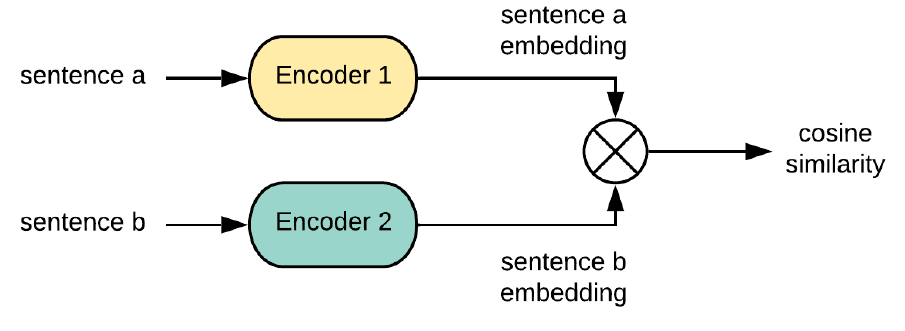
\includegraphics[width=0.68\linewidth]{figures/cf04_cosine_encoder_diagram.png}
  \caption{Schema della CosineEmbeddingLoss: due input (\textit{sentence a} e
           \textit{sentence b}) vengono proiettati attraverso due encoder e i
           rispettivi embedding vengono confrontati tramite cosine similarity.
           Il simbolo $\otimes$ indica il prodotto scalare normalizzato.}
  \label{fig:cosine_encoder}
\end{figure}

\subsection{Interpretazione Geometrica}
\label{subsec:cosine-geometry}

$1 - \cos(\theta)$ tra due vettori è equivalente alla \textbf{distanza euclidea
normalizzata}: dopo aver portato i vettori sulla sfera unitaria, la loro distanza
dipende solo dall'angolo $\theta$ tra loro, non dalla loro norma.

\begin{figure}[H]
  \centering
  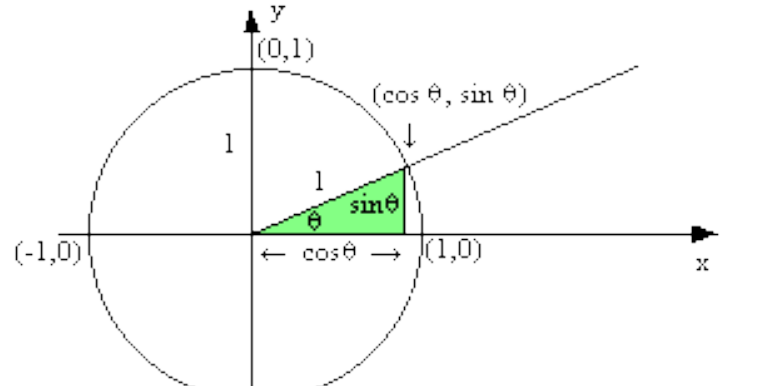
\includegraphics[width=0.52\linewidth]{figures/cf04_cosine_unit_circle.png}
  \caption{Cerchio unitario: il punto $(\cos\theta, \sin\theta)$ giace sulla
           sfera unitaria. La distanza coseno $1 - \cos\theta$ misura quanto
           due vettori normalizzati differiscono in direzione, indipendentemente
           dalla loro magnitudine.}
  \label{fig:cosine_circle}
\end{figure}

\paragraph{Perché normalizzare?}
Se si vuole massimizzare la distanza tra vettori dissimili, la rete potrebbe
semplicemente allungare i vettori anziché ruotarli nella direzione corretta.
La normalizzazione forza la rete a \textbf{ruotare} i vettori, non a scalarne
la norma. In uno spazio ad alta dimensione, la maggior parte dell'``area'' della
sfera si trova vicino all'equatore: dopo la normalizzazione, campioni semanticamente
simili devono stare vicini sulla sfera, quelli dissimili devono essere
\textbf{ortogonali}.

\paragraph{Comportamento per le due casistiche:}
\begin{itemize}
  \item \textbf{Coppie positive} ($y=1$): la loss cerca di allineare i vettori
        il più possibile ($\cos\theta \to 1$).
  \item \textbf{Coppie negative} ($y=-1$): la loss spinge il coseno sotto un
        margine positivo piccolo, rendendo i vettori ortogonali o opposti.
\end{itemize}

%------------------------------------------------------------
\section{Guida Pratica alla Scelta della Loss}
\label{sec:loss-guide}

\begin{table}[H]
  \centering
  \caption{Guida alla scelta della funzione di perdita.}
  \label{tab:loss_guide}
  \small
  \begin{tabularx}{\linewidth}{l l X}
    \toprule
    \textbf{Task} & \textbf{Loss consigliata} & \textbf{Note} \\
    \midrule
    Regressione standard        & \texttt{MSELoss}             & Sensibile agli outlier \\
    Regressione robusta         & \texttt{SmoothL1Loss}        & Huber, usata in CV \\
    Regressione con immagini    & \texttt{L1Loss}              & Predizioni più nitide \\
    Classificazione multiclasse & \texttt{CrossEntropyLoss}    & Input = logit grezzi \\
    Classificazione binaria     & \texttt{BCEWithLogitsLoss}   & Numericamente stabile \\
    Classi sbilanciate          & \texttt{NLLLoss} + weight    & O equalizzare frequenza \\
    Classi $\gg 10^4$           & \texttt{AdaptiveLogSoftmax}  & Approssimazione efficiente \\
    Ranking / retrieval         & \texttt{MarginRankingLoss}   & Coppia positivo/negativo \\
    Metric learning             & \texttt{TripletMarginLoss}   & Tripla anchor/pos/neg \\
    Embedding similarity        & \texttt{CosineEmbeddingLoss} & Direzione vettoriale \\
    \bottomrule
  \end{tabularx}
\end{table}

\paragraph{Regole operative.}
\begin{enumerate}
  \item Usare sempre \texttt{nn.CrossEntropyLoss} (non \texttt{Softmax} +
        \texttt{NLLLoss} separatamente) per stabilità numerica del gradiente.
  \item Per classificazione binaria preferire \texttt{BCEWithLogitsLoss}
        a \texttt{BCELoss}: non richiedere che l'output sia già in $(0,1)$.
  \item In computer vision generativa (super-risoluzione, inpainting) preferire
        L1 a L2 per evitare immagini sfocate.
  \item Per dataset sbilanciati, privilegiare l'equalizzazione della frequenza
        sui buffer rispetto ai pesi nella loss, e fare fine-tuning finale con la
        distribuzione reale.
  \item Nelle loss basate su margine, scegliere il valore del margine tramite
        validation set: un margine troppo piccolo produce scarsa separazione, uno
        troppo grande può impedire la convergenza.
\end{enumerate}

%------------------------------------------------------------
\section{Riepilogo}
\label{sec:summary-ch4}

\begin{center}
\small
\begin{tabular}{lll}
  \toprule
  \textbf{Categoria} & \textbf{Loss} & \textbf{Proprietà chiave} \\
  \midrule
  Regressione   & MSE               & Media, sensibile outlier \\
                & L1                & Mediana, robusta, non diff.\ in 0 \\
                & SmoothL1 (Huber)  & L2 vicino a 0, L1 lontano \\
  \midrule
  Classificazione & CrossEntropyLoss & LogSoftmax + NLL fusi \\
                  & BCEWithLogitsLoss & Sigmoid + BCE fusi \\
                  & NLLLoss           & Con pesi per classi sbilanciate \\
                  & KLDivLoss         & Distanza tra distribuzioni \\
  \midrule
  Margine       & HingeEmbedding    & Similarità/dissimilarità \\
                & MarginRanking     & Ordinamento relativo \\
                & TripletMargin     & Anchor/Positivo/Negativo \\
                & CosineEmbedding   & Similarità angolare normalizzata \\
  \bottomrule
\end{tabular}
\end{center}

La scelta della loss non è separabile dall'architettura: \texttt{CrossEntropyLoss}
richiede logit grezzi in input (non una Softmax esplicita), \texttt{BCEWithLogitsLoss}
richiede logit (non probabilità), e le loss basate su margine operano su coppie o
triple che devono essere costruite correttamente nel DataLoader.
Come sottolinea \citet{bishop2024}, la loss function codifica l'assunzione
probabilistica sul rumore del dato: MSE corrisponde a un modello gaussiano,
L1 a un modello laplaciano, e la Cross-Entropy al massimo della
verosimiglianza per distribuzioni categoriali.

%============================================================
%  Capitolo 5 – Ottimizzazione
%============================================================
\chapter{Ottimizzazione}
\label{ch:optimization}

L'ottimizzazione è il processo che permette alla rete neurale di apprendere,
aggiornando iterativamente i parametri $\mathbf{w}$ in modo da minimizzare la
funzione di perdita $\mathcal{L}$. A differenza dell'ottimizzazione classica, in
Deep Learning la funzione obiettivo è \emph{non convessa}, ad alta dimensionalità
e valutatata su dati rumorosi campionati in mini-batch. La comprensione della
geometria della superficie di errore e dei metodi per percorrerla efficientemente
è fondamentale tanto quanto la scelta dell'architettura \citep{bishop2024}.

%------------------------------------------------------------
\section{La Superficie di Errore}
\label{sec:error-surface}

\subsection{Neuroni Lineari e Ciotola Quadratica}
\label{subsec:quadratic-bowl}

La \textbf{superficie di errore} vive in uno spazio con un asse orizzontale per
ogni peso e un asse verticale per il valore della loss. Per un neurone lineare
con errore quadratico medio la superficie è una \textbf{ciotola quadratica}
(quadratic bowl):

\begin{itemize}
  \item Le sezioni verticali sono \textbf{parabole}.
  \item Le sezioni orizzontali sono \textbf{ellissi} (o cerchi se il problema
        è ben condizionato).
\end{itemize}

Per reti multi-layer non lineari la superficie è molto più complessa, ma
\emph{localmente} una ciotola quadratica rimane un'ottima approssimazione.

\begin{figure}[H]
  \centering
  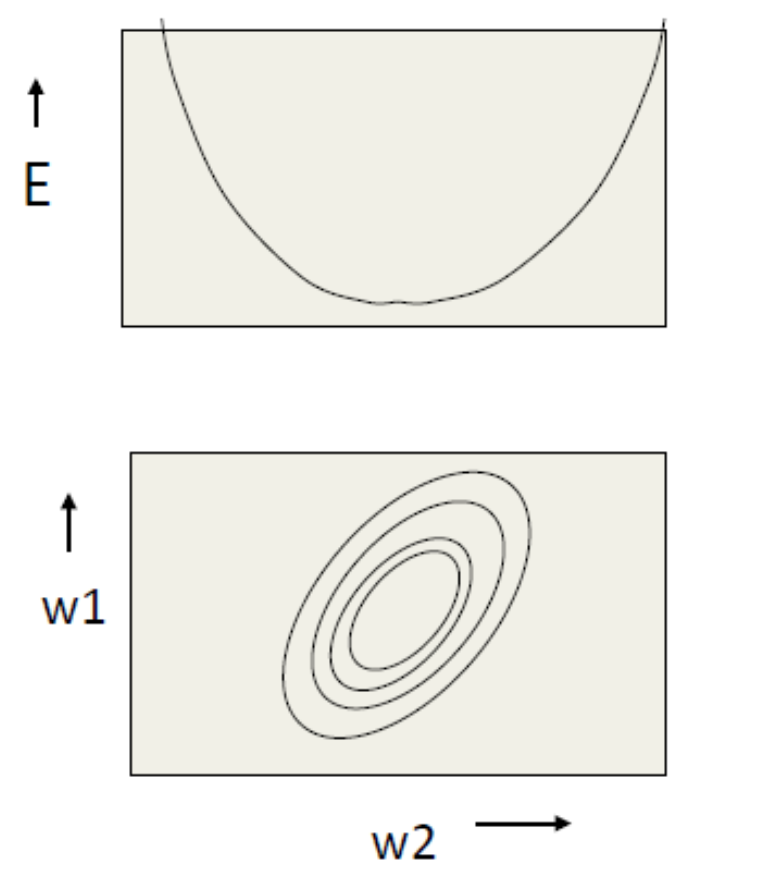
\includegraphics[width=0.72\linewidth]{figures/cf05_error_surface_bowl.png}
  \caption{Sinistra: sezione verticale della superficie di errore per un
           neurone lineare (parabola). Destra: sezione orizzontale (ellissi
           concentriche) nello spazio dei pesi $w_1$--$w_2$.}
  \label{fig:error_surface}
\end{figure}

\subsection{Il Problema della Direzione del Gradiente}
\label{subsec:gradient-direction}

Nella discesa del gradiente si scende lungo la direzione di massima pendenza,
ma questo non coincide con la direzione verso il minimo salvo che le ellissi
siano cerchi. Il problema nasce perché:

\begin{itemize}
  \item Il gradiente è \textbf{grande} nella direzione in cui vogliamo percorrere
        una piccola distanza (curvatura elevata).
  \item Il gradiente è \textbf{piccolo} nella direzione in cui vogliamo percorrere
        una grande distanza (curvatura bassa).
\end{itemize}

Questa asimmetria rende la convergenza lenta e produce i caratteristici
\emph{zig-zag} osservabili nelle traiettorie di ottimizzazione su superfici
ellittiche.

%------------------------------------------------------------
\section{Algoritmi di Apprendimento: Batch, Mini-Batch, Online}
\label{sec:learning-algorithms}

\subsection{Ridondanza nel Dataset}
\label{subsec:redundancy}

Quando il dataset è \textbf{altamente ridondante}, il gradiente calcolato sulla
prima metà dei dati è quasi identico a quello calcolato sulla seconda metà. In
questo caso conviene aggiornare i pesi più volte per epoch, anziché attendere il
calcolo del gradiente completo.

\begin{description}
  \item[Full Batch] Il gradiente viene calcolato sull'intero dataset. Sono
        disponibili metodi più sofisticati (gradiente coniugato non lineare,
        L-BFGS) ma il costo per iterazione è elevato.
  \item[Online (SGD puro)] Il peso viene aggiornato dopo ogni singolo esempio.
        Noisy ma veloce nelle prime fasi.
  \item[Mini-Batch] Compromesso ottimale per reti grandi: si calcola il gradiente
        su un sottoinsieme $B$ di esempi. Sfrutta la moltiplicazione
        matrice-matrice accelerata da GPU e bilancia rumore e costo computazionale.
\end{description}

\paragraph{Regola pratica.}
Per reti neurali grandi su dataset grandi e ridondanti il \textbf{mini-batch} è
quasi sempre la scelta migliore \citep{bishop2024}. I mini-batch devono essere
bilanciati tra le classi per evitare gradienti sistematicamente distorti.

%------------------------------------------------------------
\section{Accorgimenti per il Mini-Batch Gradient Descent}
\label{sec:tricks-minibatch}

\subsection{Learning Rate e Quando Ridurlo}
\label{subsec:lr-schedule}

Abbassare il learning rate $\eta$ durante l'addestramento riduce le fluttuazioni
casuali della loss dovute ai diversi gradienti sui diversi mini-batch:

\begin{itemize}
  \item Si ottiene un \emph{guadagno rapido} nel breve periodo (la loss scende
        più liscia).
  \item Si rallenta però l'apprendimento nel lungo periodo.
\end{itemize}

\begin{figure}[H]
  \centering
  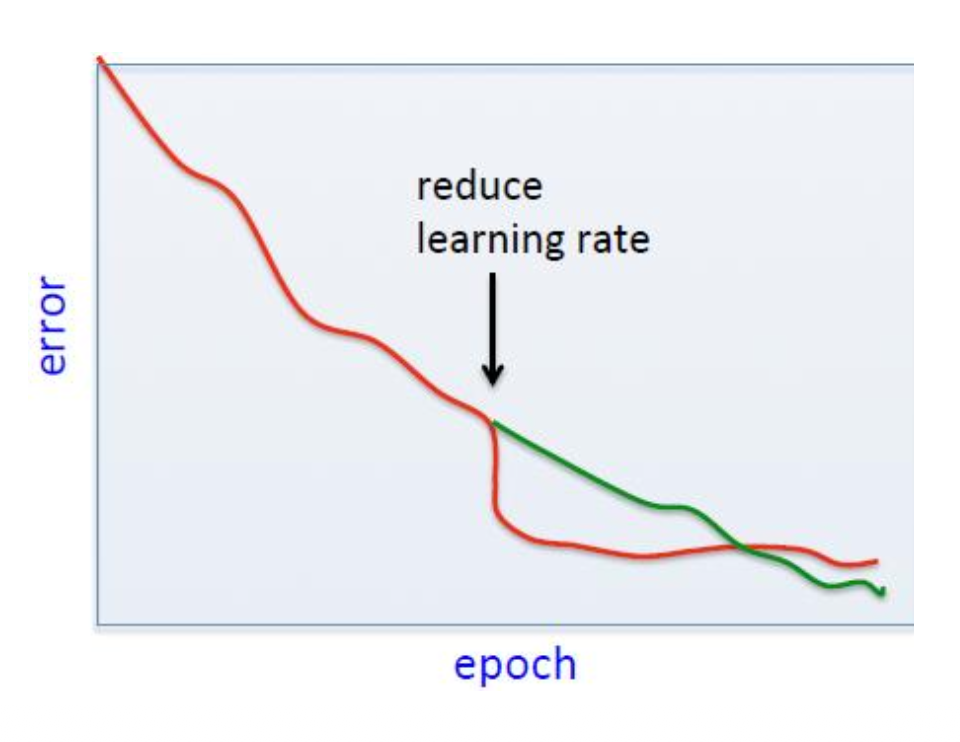
\includegraphics[width=0.60\linewidth]{figures/cf05_lr_schedule.png}
  \caption{Effetto della riduzione del learning rate sulla curva di addestramento.
           La riduzione prematura (rosso) porta a convergenza lenta; quella
           ritardata (verde) sfrutta le oscillazioni iniziali per esplorare meglio
           lo spazio dei parametri.}
  \label{fig:lr_schedule}
\end{figure}

\textbf{Non ridurre il learning rate troppo presto!}

\subsection{Inizializzazione dei Pesi}
\label{subsec:weight-init}

Se due unità nascoste hanno esattamente lo stesso bias e gli stessi pesi in
ingresso e in uscita, riceveranno sempre lo stesso gradiente e non potranno mai
imparare feature diverse. Questo problema, detto \emph{symmetry breaking},
si risolve inizializzando i pesi con valori casuali piccoli.

\paragraph{Fan-in e overshooting.}
Un'unità con fan-in elevato (molti ingressi) può subire un effetto di
\emph{overshoot}: piccole variazioni su molti pesi in ingresso si sommano,
spostando eccessivamente l'uscita. La regola empirica è:

\begin{equation}
  w \propto \frac{\mathcal{N}(0,1)}{\sqrt{n_{\text{in}}}},
\end{equation}

dove $n_{\text{in}}$ è il numero di connessioni in ingresso (fan-in).

\subsubsection{Inizializzazione di Xavier / Glorot}
\label{subsubsec:xavier}

\citet{glorot2010} hanno mostrato che, per preservare la varianza dei segnali
sia in forward che in backward pass, conviene tenere conto sia del fan-in che del
fan-out. Per una distribuzione \textbf{uniforme} $\mathcal{U}(-a, a)$:

\begin{equation}
  a = \text{gain} \times \sqrt{\frac{6}{n_{\text{in}} + n_{\text{out}}}},
\end{equation}

mentre per una distribuzione \textbf{normale} $\mathcal{N}(0, \sigma^2)$:

\begin{equation}
  \sigma = \text{gain} \times \sqrt{\frac{2}{n_{\text{in}} + n_{\text{out}}}}.
\end{equation}

Il parametro \texttt{gain} dipende dalla funzione di attivazione (es.\ $1$ per
la sigmoide, $\sqrt{5}$ per ReLU nella variante He). In PyTorch:
\texttt{nn.init.xavier\_uniform\_} e \texttt{nn.init.xavier\_normal\_}.

\subsection{Pre-elaborazione degli Input}
\label{subsec:input-preprocessing}

Traslare e scalare gli input (\emph{shift and scale}) in modo che abbiano
media zero e varianza unitaria rende la superficie di errore più \emph{circolare}
(meno ellittica), migliorando la velocità di convergenza. Un approccio più
avanzato è la \textbf{decorrelazione} tramite PCA:

\begin{enumerate}
  \item Eliminare le componenti principali con autovalori più piccoli
        (riduzione della dimensionalità).
  \item Dividere le componenti rimanenti per la radice quadrata dei rispettivi
        autovalori (\emph{whitening}).
\end{enumerate}

Per un neurone lineare, il whitening converte la superficie di errore da
un'ellissi allineata agli assi a un cerchio, rendendo ottimale la discesa del
gradiente puro.

%------------------------------------------------------------
\section{Il Metodo del Momentum}
\label{sec:momentum}

\subsection{Intuizione Fisica}
\label{subsec:momentum-intuition}

L'idea del momentum si ispira alla fisica classica: immaginiamo una pallina che
rotola sulla superficie di errore. La posizione della pallina nel piano
orizzontale rappresenta il vettore dei pesi. Inizialmente la pallina segue il
gradiente, ma non appena acquisisce velocità smette di seguire la direzione di
massima pendenza: il \emph{momentum} la trascina nella direzione in cui si stava
già muovendo.

\begin{figure}[H]
  \centering
  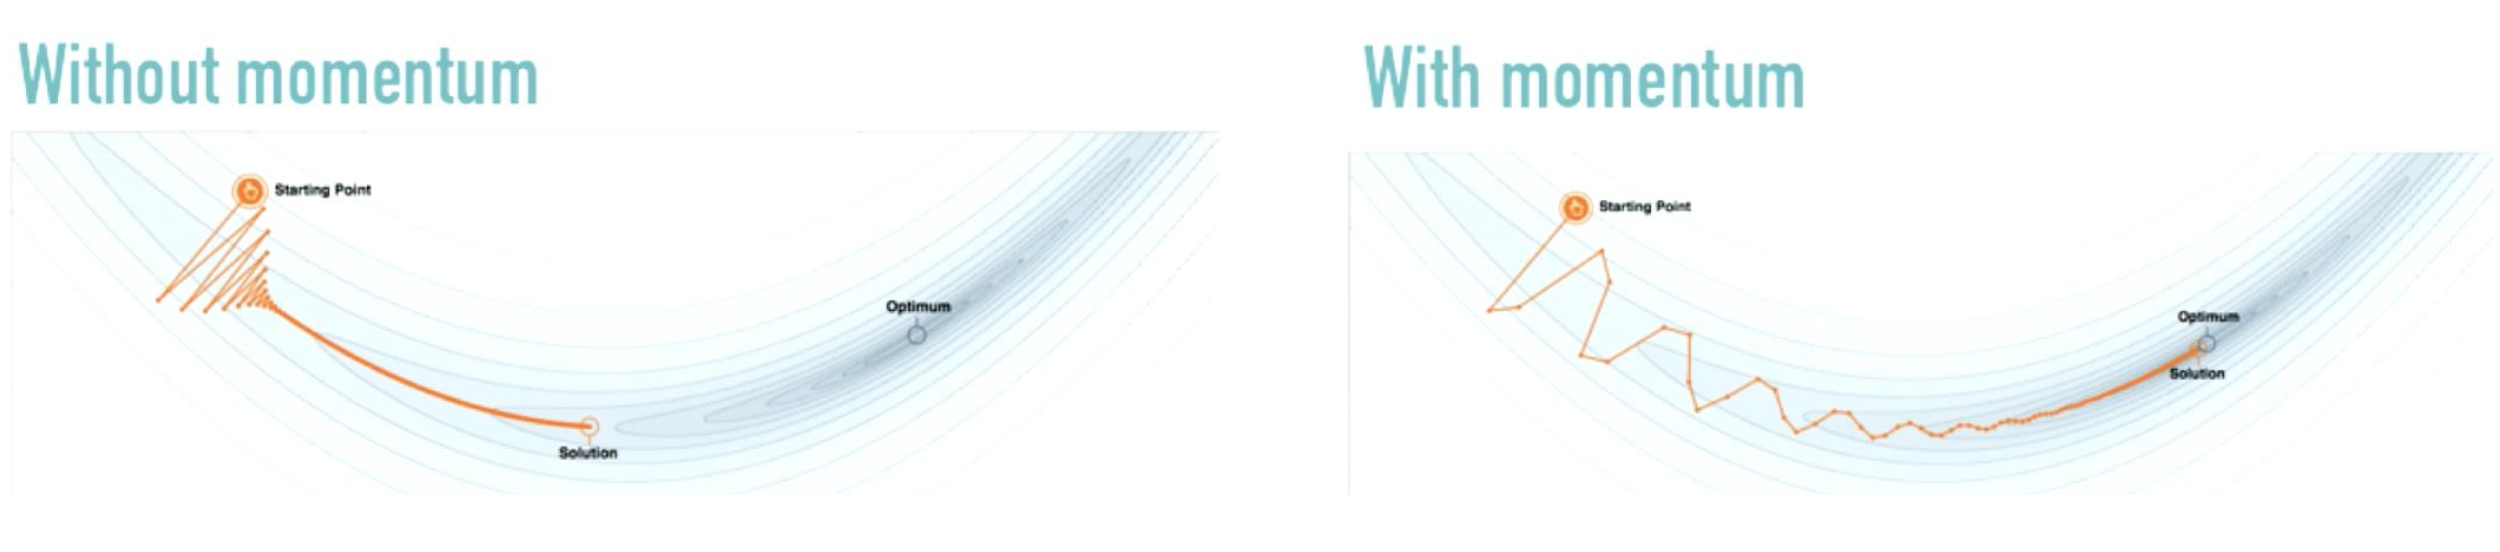
\includegraphics[width=0.75\linewidth]{figures/cf05_momentum_comparison.png}
  \caption{Confronto tra SGD senza momentum (sinistra) e con momentum (destra).
           Senza momentum la traiettoria oscilla fortemente in direzione
           trasversale; con momentum le oscillazioni vengono smorzate e la
           discesa verso il minimo è più diretta.}
  \label{fig:momentum_comparison}
\end{figure}

I benefici principali sono due:
\begin{itemize}
  \item \textbf{Smorzamento delle oscillazioni} nelle direzioni ad alta curvatura,
        combinando gradienti con segno opposto.
  \item \textbf{Accelerazione} nelle direzioni a gradiente piccolo ma consistente.
\end{itemize}

\subsection{Equazioni del Momentum (SGD con Momentum)}
\label{subsec:momentum-equations}

In SGD con momentum si mantengono due quantità: il vettore dei pesi $\mathbf{w}$
e il \emph{termine di momentum} $\mathbf{p}$ (un running average dei gradienti).
Le equazioni di aggiornamento sono:

\begin{align}
  \mathbf{p}_{k+1} &= \beta\,\mathbf{p}_k + \eta\,\nabla\mathcal{L}(X, y, \mathbf{w}_k), \\
  \mathbf{w}_{k+1} &= \mathbf{w}_k - \gamma\,\mathbf{p}_{k+1},
\end{align}

dove $\beta \in (0,1)$ è il \textbf{coefficiente di smorzamento} (dampening
factor o momentum coefficient) ed $\eta$ è il learning rate. Il parametro $\beta$
deve essere strettamente maggiore di zero (altrimenti si ricade nel semplice
gradient descent) e strettamente minore di uno (altrimenti le quantità
esplodono).

\paragraph{Effetto di $\beta$.}
Valori piccoli di $\beta$ permettono di cambiare direzione più rapidamente;
valori grandi producono una traiettoria più inerziale, con curve più lente ma
smorzamento maggiore delle oscillazioni.

\subsection{Momentum di Nesterov (NAG)}
\label{subsec:nesterov}

Il metodo standard calcola il gradiente nella posizione corrente e poi compie un
grande salto. \citet{sutskever2012} ha proposto una variante ispirata al metodo
di Nesterov per funzioni convesse:

\begin{enumerate}
  \item Compie un grande salto nella direzione del gradiente \emph{accumulato
        precedentemente}.
  \item Misura il gradiente nella nuova posizione e applica una correzione.
\end{enumerate}

Le equazioni diventano:

\begin{align}
  \hat{\mathbf{w}}_k &= \mathbf{w}_k - \beta\,\mathbf{p}_k, \\
  \mathbf{p}_{k+1}   &= \beta\,\mathbf{p}_k + \eta\,\nabla\mathcal{L}(X, y,
                         \hat{\mathbf{w}}_k), \\
  \mathbf{w}_{k+1}   &= \mathbf{w}_k - \gamma\,\mathbf{p}_{k+1}.
\end{align}

\begin{figure}[H]
  \centering
  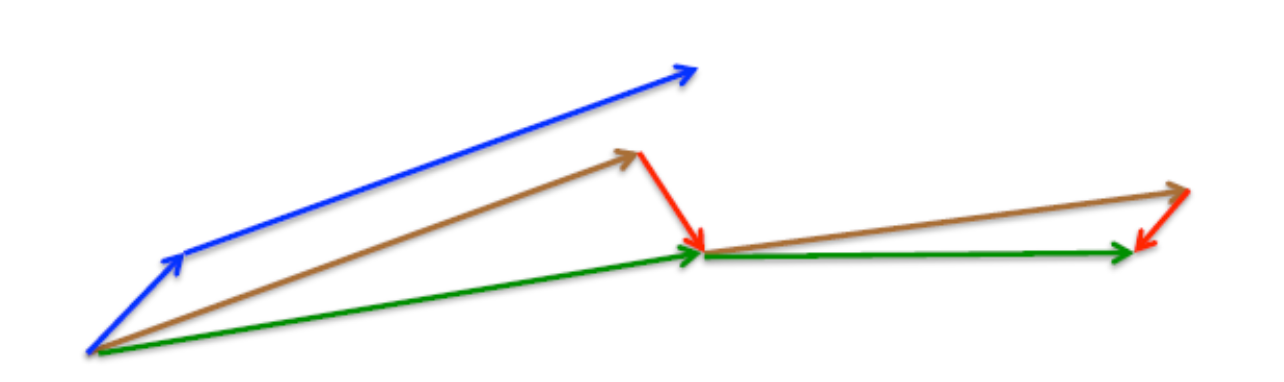
\includegraphics[width=0.55\linewidth]{figures/cf05_nesterov_vectors.png}
  \caption{Intuizione del Nesterov Accelerated Gradient. Il vettore marrone è il
           salto nella direzione accumulata, il rosso è la correzione, il verde è
           il gradiente accumulato risultante. I vettori blu rappresentano il
           percorso del momentum standard.}
  \label{fig:nesterov}
\end{figure}

\paragraph{Perché il momentum funziona?}
Esistono due spiegazioni complementari:

\begin{description}
  \item[Accelerazione] Con Nesterov è dimostrabile una convergenza accelerata su
        problemi \emph{convessi}. Per reti neurali la prova non si applica
        direttamente, e l'accelerazione regge solo su superfici quadratiche. In
        più, l'accelerazione non funziona bene in presenza di rumore stocastico.
  \item[Noise Smoothing] Ragione probabilmente più importante in pratica: il
        momentum è un \emph{running average} dei gradienti. Dove SGD richiederebbe
        di mediare molti aggiornamenti prima di fare un passo, il momentum lo fa
        automaticamente, rendendo ogni singolo aggiornamento una buona
        approssimazione della direzione corretta.
\end{description}

In sintesi, sia l'accelerazione che il noise smoothing contribuiscono alle buone
prestazioni del momentum SGD. Il noise smoothing evita il rimbalzamento sul
"pavimento" del minimo (bottom of the valley), mentre l'accelerazione velocizza
la discesa nelle regioni a bassa curvatura.

%------------------------------------------------------------
\section{Learning Rate Adattativi Separati}
\label{sec:adaptive-lr}

\subsection{Motivazione}
\label{subsec:adaptive-lr-motivation}

In una rete multi-layer i learning rate ottimali possono variare molto tra i
pesi:

\begin{itemize}
  \item Le ampiezze dei gradienti sono spesso molto diverse tra i layer,
        specialmente con pesi iniziali piccoli.
  \item Il fan-in di un'unità determina l'entità dell'effetto di overshoot
        causato dalla modifica simultanea di molti pesi in ingresso.
\end{itemize}

La strategia è usare un \textbf{learning rate globale} (impostato a mano)
moltiplicato per un \textbf{guadagno locale} $g_{ij}(t)$ determinato
empiricamente per ogni peso.

\subsection{Determinazione dei Guadagni Locali}
\label{subsec:local-gains}

Si parte da $g_{ij}(t_0) = 1$ per ogni peso. Poi, ad ogni step:

\begin{equation}
  \Delta w_{ij} = -\epsilon\, g_{ij}\, \frac{\partial E}{\partial w_{ij}}
\end{equation}

\begin{equation}
  g_{ij}(t) =
  \begin{cases}
    g_{ij}(t-1) + 0.05
      & \text{se } \dfrac{\partial E}{\partial w_{ij}}(t)\cdot
                   \dfrac{\partial E}{\partial w_{ij}}(t-1) > 0 \\[8pt]
    g_{ij}(t-1) \times 0.95
      & \text{altrimenti}
  \end{cases}
\end{equation}

Aumenti additivi e decrementi moltiplicativi garantiscono che i grandi guadagni
decadano rapidamente non appena iniziano le oscillazioni. I guadagni vengono
limitati in un intervallo ragionevole (es.\ $[0.1,\, 10]$ oppure $[0.01,\, 100]$).

\begin{tcolorbox}[colback=blue!5!white, colframe=blue!50!black, title=Analogia: AIMD nel controllo della congestione TCP]
Il meccanismo di aumento additivo e decremento moltiplicativo (AIMD) è lo stesso
principio usato nel controllo della congestione TCP: aumenta linearmente la
finestra di congestione finché non si verifica una perdita, poi la dimezza.
Questo garantisce robustezza e veloce recupero dalle oscillazioni.
\end{tcolorbox}

\paragraph{Combinare con il momentum.}
I learning rate adattativi possono essere combinati con il momentum usando
l'accordo di segno tra il gradiente corrente e la velocità del peso
(Jacobs, 1989). Nota che i learning rate adattativi gestiscono solo effetti
allineati agli assi (derivate parziali), mentre il momentum non dipende
dall'allineamento degli assi.

%------------------------------------------------------------
\section{rprop e rmsprop}
\label{sec:rprop-rmsprop}

\subsection{rprop: Solo il Segno del Gradiente}
\label{subsec:rprop}

Quando l'ampiezza del gradiente varia molto tra pesi diversi e durante
l'addestramento, è difficile scegliere un unico learning rate globale. Per il
\textbf{full batch learning} si può ovviare usando solo il \emph{segno} del
gradiente:

\begin{itemize}
  \item Tutti gli aggiornamenti di peso hanno la stessa ampiezza.
  \item Si esce rapidamente dalle regioni a gradiente quasi nullo (plateau).
\end{itemize}

\textbf{rprop} combina l'uso del solo segno del gradiente con l'adattamento
della dimensione del passo per ogni peso separatamente:

\begin{itemize}
  \item Se i segni degli ultimi due gradienti \emph{concordano}: moltiplica la
        dimensione del passo per $1.2$.
  \item Altrimenti: moltiplica per $0.5$.
  \item Limita la dimensione del passo nell'intervallo $[10^{-6},\, 50]$.
\end{itemize}

\paragraph{Perché rprop non funziona con i mini-batch.}
SGD media implicitamente i gradienti su mini-batch successivi (quando il
learning rate è piccolo). rprop, invece, aggiorna la dimensione del passo sulla
base del \emph{segno} in ogni mini-batch separatamente. Se un peso riceve
gradiente $+0.1$ per nove mini-batch e $-0.9$ per uno, rprop incrementerebbe il
peso nove volte e lo decrementerà una sola volta, portando a un'esplosione del
peso. Questo motiva la necessità di rmsprop.

\subsection{rmsprop: Versione Mini-Batch di rprop}
\label{subsec:rmsprop}

\textbf{rmsprop} mantiene una media mobile del quadrato del gradiente per ogni
peso e divide il gradiente per la radice di questa media:

\begin{equation}
  \text{MeanSquare}(w, t) =
    0.9\;\text{MeanSquare}(w, t-1) + 0.1\left(\frac{\partial E}{\partial w}\right)^2,
\end{equation}

\begin{equation}
  \Delta w = -\frac{\eta}{\sqrt{\text{MeanSquare}(w,t)}}\;\frac{\partial E}{\partial w}.
\end{equation}

Dividere per $\sqrt{\text{MeanSquare}(w,t)}$ normalizza il gradiente rispetto
alla sua ampiezza recente, ottenendo l'effetto di rprop ma in modo compatibile
con i mini-batch. I valori suggeriti da Hinton sono $\gamma = 0.9$ e
$\eta = 0.001$.

%------------------------------------------------------------
\section{Metodi Adattativi Avanzati}
\label{sec:advanced-adaptive}

\subsection{Adagrad}
\label{subsec:adagrad}

\textbf{Adagrad} adatta il learning rate a ciascun parametro, effettuando
aggiornamenti più grandi per parametri rari e più piccoli per quelli frequenti.
Definendo $g_{t,i} = \nabla_\theta J(\theta_{t,i})$, l'aggiornamento SGD
standard diventa:

\begin{equation}
  \theta_{t+1,i} = \theta_{t,i} - \frac{\eta}{\sqrt{G_{t,ii} + \epsilon}}
                   \cdot g_{t,i},
\end{equation}

dove $G_t \in \mathbb{R}^{d \times d}$ è una matrice diagonale il cui elemento
$(i,i)$ è la \textbf{somma dei quadrati di tutti i gradienti passati} rispetto
a $\theta_i$ fino al passo $t$, e $\epsilon \approx 10^{-8}$ evita la
divisione per zero.

\paragraph{Vantaggi e limiti.}
Adagrad elimina la necessità di regolare manualmente il learning rate (default
$0.01$). Il limite principale è che la somma dei gradienti al quadrato cresce
monotonamente: il learning rate si riduce fino a diventare infinitesimo,
bloccando l'apprendimento.

\subsection{Adadelta}
\label{subsec:adadelta}

\textbf{Adadelta} risolve il problema di Adagrad sostituendo la somma
cumulativa dei quadrati del gradiente con una \emph{media esponenzialmente
decrescente}:

\begin{equation}
  E[g^2]_t = \gamma\, E[g^2]_{t-1} + (1-\gamma)\, g_t^2.
\end{equation}

L'aggiornamento diventa:

\begin{equation}
  \theta_{t+1,i} = \theta_{t,i} - \frac{\text{RMS}[\Delta\theta]_{t-1}}
                                        {\text{RMS}[g]_t}\, g_t,
\end{equation}

dove $\text{RMS}[g]_t = \sqrt{E[g^2]_t + \epsilon}$ e
$\text{RMS}[\Delta\theta]_{t-1}$ è la radice del mean square degli aggiornamenti
passati (anch'esso calcolato con media esponenziale). In questo modo il learning
rate viene eliminato dall'equazione e non deve essere impostato.

\paragraph{Relazione con rmsprop.}
RMSprop e Adadelta sono stati sviluppati indipendentemente nello stesso periodo
per risolvere lo stesso problema. RMSprop corrisponde esattamente al primo
vettore di aggiornamento di Adadelta.

\subsection{Adam: Adaptive Moment Estimation}
\label{subsec:adam}

\textbf{Adam} \citep{kingma2014adam} combina l'idea di rmsprop (media del quadrato
dei gradienti) con quella del momentum (media dei gradienti), mantenendo stime
del \emph{primo momento} (media) e del \emph{secondo momento non centrato}
(varianza) dei gradienti:

\begin{align}
  m_t &= \beta_1\, m_{t-1} + (1-\beta_1)\, g_t, \\
  v_t &= \beta_2\, v_{t-1} + (1-\beta_2)\, g_t^2.
\end{align}

Poiché $m_0 = v_0 = \mathbf{0}$, le stime sono distorte verso zero nelle prime
iterazioni. Si correggono con:

\begin{equation}
  \hat{m}_t = \frac{m_t}{1 - \beta_1^t}, \qquad
  \hat{v}_t = \frac{v_t}{1 - \beta_2^t}.
\end{equation}

L'aggiornamento finale è:

\begin{equation}
  \theta_{t+1} = \theta_t - \frac{\eta}{\sqrt{\hat{v}_t} + \epsilon}\,\hat{m}_t.
\end{equation}

I valori di default suggeriti dagli autori sono $\beta_1 = 0.9$,
$\beta_2 = 0.999$, $\epsilon = 10^{-8}$.

\paragraph{Interpretazione.}
Quando i gradienti rimangono approssimativamente costanti (discesa uniforme),
la varianza è quasi nulla e $v_t \approx m_t^2$, quindi
$\hat{m}_t / \sqrt{\hat{v}_t} \approx 1$: il passo è dell'ordine di $\eta$.
Quando i gradienti cambiano rapidamente, $\sqrt{\hat{v}_t} \gg \hat{m}_t$ e il
passo diventa molto più piccolo di $\eta$. Adam adatta quindi la dimensione del
passo in modo automatico per ciascun peso.

\begin{figure}[H]
  \centering
  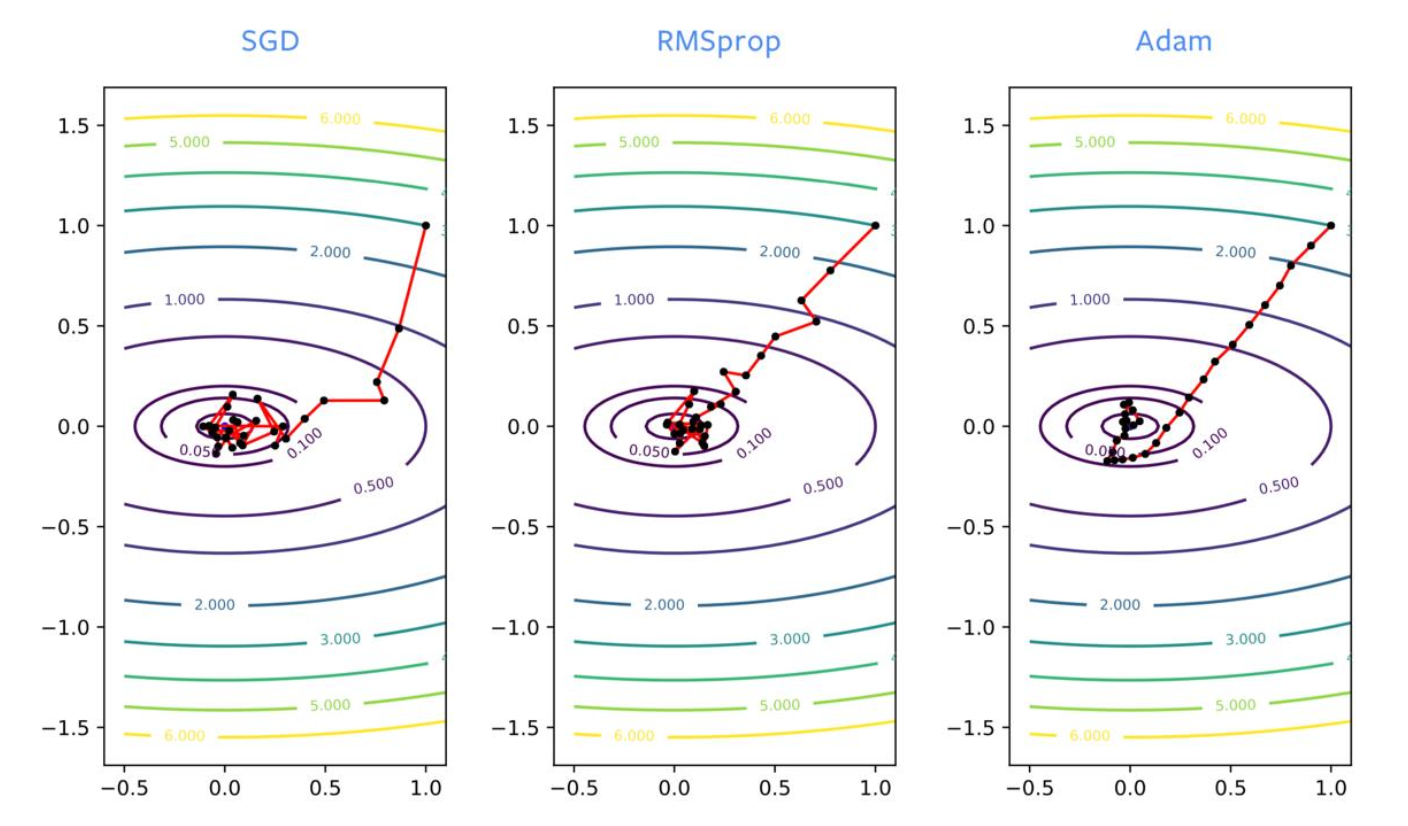
\includegraphics[width=0.88\linewidth]{figures/cf05_sgd_rmsprop_adam.png}
  \caption{Confronto delle traiettorie di SGD, RMSprop e Adam sulla stessa
           superficie di errore. Adam converge in modo più diretto verso il
           minimo grazie alla combinazione di momentum e normalizzazione
           adattiva.}
  \label{fig:sgd_vs_adam}
\end{figure}

\subsubsection{Limitazioni di Adam}
\label{subsubsec:adam-limits}

\begin{itemize}
  \item Su problemi semplici è dimostrabile che Adam \textbf{non converge}.
  \item Tende a produrre \textbf{errori di generalizzazione} maggiori rispetto a
        SGD, specialmente in computer vision: trovare il minimo locale più vicino
        (invece del minimo "piatto" favorito da SGD) porta a minori capacità di
        generalizzazione.
  \item Richiede \textbf{3 buffer} invece di 1 (pesi, $m_t$, $v_t$): per modelli
        da miliardi di parametri questo può diventare limitante in memoria.
  \item Sono necessari 2 iperparametri di momentum da regolare invece di 1.
\end{itemize}

\subsection{AdamW: Adam con Weight Decay Corretto}
\label{subsec:adamw}

Le librerie di deep learning implementano tipicamente la \emph{L2
regularization} aggiungendo $\lambda\, w$ al gradiente prima dell'aggiornamento.
Tuttavia questo non è equivalente al weight decay per gli ottimizzatori
adattativi: il termine di regolarizzazione viene normalizzato da $\sqrt{v_t}$,
quindi i pesi con gradienti grandi vengono regolarizzati \emph{meno} di quelli
con gradienti piccoli. \textbf{AdamW} separa il weight decay dall'aggiornamento
adattivo:

\begin{equation}
  \mathbf{x}_t \leftarrow \mathbf{x}_{t-1}
    - \eta_t \left(\frac{\alpha\,\hat{m}_t}{\sqrt{\hat{v}_t} + \epsilon}\right)
    - \eta_t\, w\, \mathbf{x}_{t-1}.
\end{equation}

Il termine di regolarizzazione $w\,\mathbf{x}_{t-1}$ è proporzionale al solo
valore del peso e non viene influenzato dalla normalizzazione adattiva,
replicando il comportamento del weight decay in SGD e migliorando la
generalizzazione.

\subsection{Lion: EvoLved Sign Momentum}
\label{subsec:lion}

\textbf{Lion} \citep{chen2023lion} è un ottimizzatore scoperto tramite
\emph{program search} (ricerca evolutiva sullo spazio dei programmi). Richiede
meno memoria di Adam (mantiene solo il momentum, non il secondo momento) e
produce aggiornamenti di ampiezza uniforme grazie all'operazione \texttt{sign}:

\begin{lstlisting}[language=Python, caption={Pseudocodice di Lion.}, label={lst:lion}]
def train(weight, gradient, momentum, lr):
    update   = interp(gradient, momentum, beta1)  # (1-b1)*m + b1*g
    update   = sign(update)
    momentum = interp(gradient, momentum, beta2)
    update   = update + weight * lambda_wd         # weight decay
    update   = update * lr
    return update, momentum
\end{lstlisting}

Le prestazioni di Lion crescono con la dimensione del mini-batch e richiedono un
learning rate più piccolo rispetto ad Adam a causa della norma maggiore prodotta
dalla funzione \texttt{sign}.

%------------------------------------------------------------
\section{Metodi di Secondo Ordine}
\label{sec:second-order}

\subsection{Riduzione dell'Errore e Rapporto Gradiente/Curvatura}
\label{subsec:gradient-curvature}

La riduzione massima dell'errore percorrendo una direzione $\mathbf{d}$ dipende
dal \textbf{rapporto gradiente/curvatura}. Una buona direzione ha un rapporto
elevato anche se il gradiente è piccolo. Per trovare queste direzioni si può
usare la matrice di curvatura (Hessiana):

\begin{equation}
  H_{i,j} = \frac{\partial^2 f}{\partial x_i \partial x_j}.
\end{equation}

\begin{description}
  \item[Gradiente] Vettore delle derivate prime di un campo scalare.
  \item[Jacobiano] Matrice dei gradienti per le componenti di un campo vettoriale
        ($J_{i,j} = \partial F_i / \partial x_j$).
  \item[Hessiana] Matrice delle derivate miste di secondo ordine di un campo
        scalare.
\end{description}

\subsection{Metodo di Newton}
\label{subsec:newton}

Il metodo di Newton moltiplica il vettore del gradiente per l'inversa della
matrice di curvatura $H$:

\begin{equation}
  \Delta \mathbf{w} = -\epsilon\, H(\mathbf{w})^{-1}\, \frac{dE}{d\mathbf{w}}.
\end{equation}

Su una superficie quadratica reale converge al minimo in un unico passo. Il
problema pratico è che con un milione di pesi la matrice di curvatura ha un
trilione di termini: \textbf{inverirla è computazionalmente intrattabile}.

\paragraph{Matrici di curvatura.}
Ogni elemento della matrice specifica come il gradiente in una direzione cambia
spostandosi in un'altra. I termini fuori diagonale corrispondono alle
\emph{torsioni} della superficie di errore. La ragione per cui la discesa del
gradiente produce zig-zag è che aggiornare un peso muta il gradiente di tutti
gli altri.

\subsection{Hessian-Free Optimization e Gradiente Coniugato}
\label{subsec:hessian-free}

Il metodo \textbf{Hessian-Free} (HF) approssima la matrice di curvatura e,
assumendo che quell'approssimazione sia corretta, minimizza l'errore usando il
\textbf{gradiente coniugato} (CG). Poi aggiorna l'approssimazione e minimizza di
nuovo.

\paragraph{Gradiente Coniugato.}
Invece di invertire $H$ in un solo passo, CG usa una sequenza di passi ognuno
dei quali minimizza l'errore lungo una direzione:

\begin{itemize}
  \item Ogni nuova direzione è \emph{coniugata} alle precedenti: muoversi in
        essa non altera i gradienti nelle direzioni già ottimizzate.
  \item Dopo $N$ passi è garantita la convergenza al minimo di una superficie
        quadratica $N$-dimensionale.
  \item Applicato a superfici non quadratiche (CG non lineare) funziona comunque
        bene nella pratica.
\end{itemize}

L'ottimizzatore HF usa CG sulla superficie quadratica approssimata (dove CG è
ottimale). Per le RNN è importante aggiungere un vincolo che impedisce di
modificare troppo le attività nascoste da un'iterazione all'altra.

%------------------------------------------------------------
\section{Riepilogo dei Metodi di Ottimizzazione}
\label{sec:optim-summary}

\begin{table}[H]
  \centering
  \caption{Guida alla scelta dell'ottimizzatore.}
  \label{tab:optim_guide}
  \small
  \begin{tabular}{lll}
    \toprule
    \textbf{Scenario} & \textbf{Ottimizzatore} & \textbf{Note} \\
    \midrule
    Dataset piccolo ($\leq$10k) / bassa ridondanza
      & Full-batch (CG, L-BFGS, rprop)
      & Convergenza precisa \\
    Dataset grande e ridondante
      & Mini-batch SGD + Momentum
      & Default per CV \\
    Gradient sparso / NLP / embedding
      & Adam / AdamW
      & Adattività per feature rare \\
    Modelli grandi, generalizzazione critica
      & AdamW o SGD + momentum
      & AdamW corregge weight decay \\
    Memoria limitata, batch grande
      & Lion
      & Un solo buffer di stato \\
    \bottomrule
  \end{tabular}
\end{table}

\paragraph{Regole operative.}
\begin{enumerate}
  \item Inizializzare i pesi con \textbf{Xavier/Glorot} (sigmoide/tanh) o
        \textbf{He} (ReLU); mai inizializzare a zero tutti i pesi hidden.
  \item Normalizzare gli input (media zero, varianza unitaria) o usare Batch
        Normalization per accelerare la convergenza.
  \item Per reti grandi preferire \textbf{AdamW} come default; passare a SGD
        con momentum e cosine annealing per massimizzare la generalizzazione.
  \item Non abbassare il learning rate troppo presto: attendere che la loss si
        sia stabilizzata su un plateau.
  \item Usare mini-batch bilanciati tra le classi (cfr.\ Sezione
        \ref{subsec:redundancy}) e limitare la dimensione del mini-batch
        tenendo conto che batch più grandi richiedono learning rate più alti
        (linear scaling rule).
  \item Per i learning rate adattativi limitare sempre i guadagni locali in un
        intervallo ragionevole e usare mini-batch grandi per ridurre il rumore
        nelle stime dei segni del gradiente.
\end{enumerate}

Come sottolinea \citet{bishop2024}, non esiste una ricetta universale perché le
reti neurali differiscono enormemente (reti molto profonde, reti ricorrenti,
reti wide-shallow) e i task pongono requisiti diversi (accuratezza dei pesi,
presenza di feature rare, …). La scelta dell'ottimizzatore va quindi fatta
considerando congiuntamente architettura, dataset e obiettivo di generalizzazione.

%============================================================
%  Capitolo 6 – Normalization Layers
%============================================================
\chapter{Normalization Layers}
\label{ch:normalization}

I \textbf{layer di normalizzazione} sono componenti ormai indispensabili nelle
reti neurali profonde. Senza di essi, addestrare reti molto profonde è
difficoltoso: i gradienti esplodono o svaniscono, i tempi di convergenza si
allungano e la scelta del learning rate diventa critica. Questo capitolo
introduce il problema del \emph{covariate shift}, la soluzione più nota
(Batch Normalization), le varianti sviluppate per contesti diversi e una
discussione critica su \emph{perché} la normalizzazione funziona davvero
\citep{bishop2024}.

%------------------------------------------------------------
\section{Covariate Shift e Internal Covariate Shift}
\label{sec:covariate-shift}

Il \textbf{covariate shift} è un cambiamento nella distribuzione degli input
di un sistema di apprendimento: tipicamente la distribuzione durante il test
differisce da quella durante il training. Questo fenomeno danneggia le
prestazioni e viene normalmente affrontato con tecniche di \emph{domain
adaptation}.

Nelle reti neurali profonde esiste un fenomeno analogo ma interno:
l'\textbf{internal covariate shift}. Durante il training, gli aggiornamenti
dei pesi nei layer inferiori modificano continuamente la distribuzione degli
input per i layer superiori. I layer successivi devono quindi adattarsi non
solo a nuovi dati, ma a distribuzioni che cambiano ad ogni step di
ottimizzazione, rallentando significativamente il training.

%------------------------------------------------------------
\section{Batch Normalization}
\label{sec:batch-norm}

\subsection{Idea di Base}
\label{subsec:bn-idea}

La \textbf{Batch Normalization} (BN) \citep{ioffe2015batch} è un metodo di
normalizzazione applicato ai layer interni della rete. Normalmente gli input
alla rete vengono normalizzati nell'intervallo $[0,1]$ o $[-1,1]$ oppure
portati a media zero e varianza unitaria. BN estende questa pratica ai layer
intermedi, eseguendo un'\emph{operazione di whitening} sulle attivazioni
ad ogni step.

\subsection{Perché l'Approccio Naïf Non Funziona}
\label{subsec:naive-approach}

L'approccio banale sarebbe: addestrare su un batch, aggiornare i parametri,
poi normalizzare le attivazioni. Questo però \textbf{non funziona}: porta a
un'esplosione dei bias mentre i parametri di distribuzione (media e varianza)
rimangono invariati. Il motivo è che l'ottimizzazione con discesa del
gradiente non tiene conto della normalizzazione che avverrà al passo
successivo, ignorando sistematicamente il suo effetto.

\subsection{La Soluzione: un Layer di Normalizzazione Differenziabile}
\label{subsec:bn-layer}

La soluzione proposta da \citet{ioffe2015batch} è aggiungere un \textbf{layer
esplicito} che esegua la normalizzazione come parte del grafo computazionale,
in modo che il gradiente possa ``vedere'' la normalizzazione e fare
aggiustamenti se necessario.

\begin{figure}[H]
  \centering
  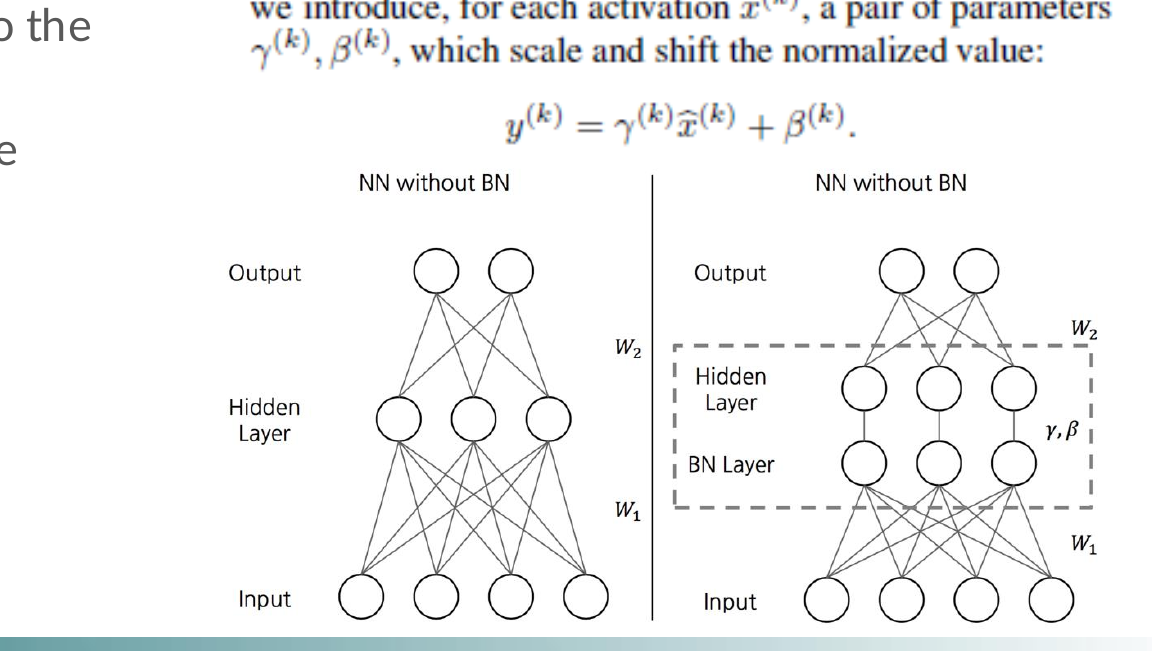
\includegraphics[width=0.72\linewidth]{figures/cf06_bn_layer_diagram.png}
  \caption{Confronto tra una rete senza BN (sinistra) e con BN (destra). Il
           BN Layer, inserito tra il layer lineare e quello successivo,
           introduce i parametri apprendibili $\gamma$ e $\beta$ che scalano
           e traslano le attivazioni normalizzate.}
  \label{fig:bn_layer_diagram}
\end{figure}

\paragraph{Algoritmo formale.}
Dato un mini-batch $\mathcal{B} = \{x_1, \ldots, x_m\}$ e i parametri
apprendibili $\gamma, \beta$, il layer BN calcola:

\begin{align}
  \mu_{\mathcal{B}}   &\leftarrow \frac{1}{m} \sum_{i=1}^{m} x_i
                       && \text{// media del mini-batch} \\[4pt]
  \sigma_{\mathcal{B}}^2 &\leftarrow \frac{1}{m} \sum_{i=1}^{m}
                           (x_i - \mu_{\mathcal{B}})^2
                       && \text{// varianza del mini-batch} \\[4pt]
  \hat{x}_i           &\leftarrow \frac{x_i - \mu_{\mathcal{B}}}
                           {\sqrt{\sigma_{\mathcal{B}}^2 + \epsilon}}
                       && \text{// normalizzazione (z-score)} \\[4pt]
  y_i                 &\leftarrow \gamma\,\hat{x}_i + \beta
                        \;\equiv\; \mathrm{BN}_{\gamma,\beta}(x_i)
                       && \text{// scala e trasla}
\end{align}

dove $\epsilon \approx 10^{-5}$ evita la divisione per zero.

\begin{figure}[H]
  \centering
  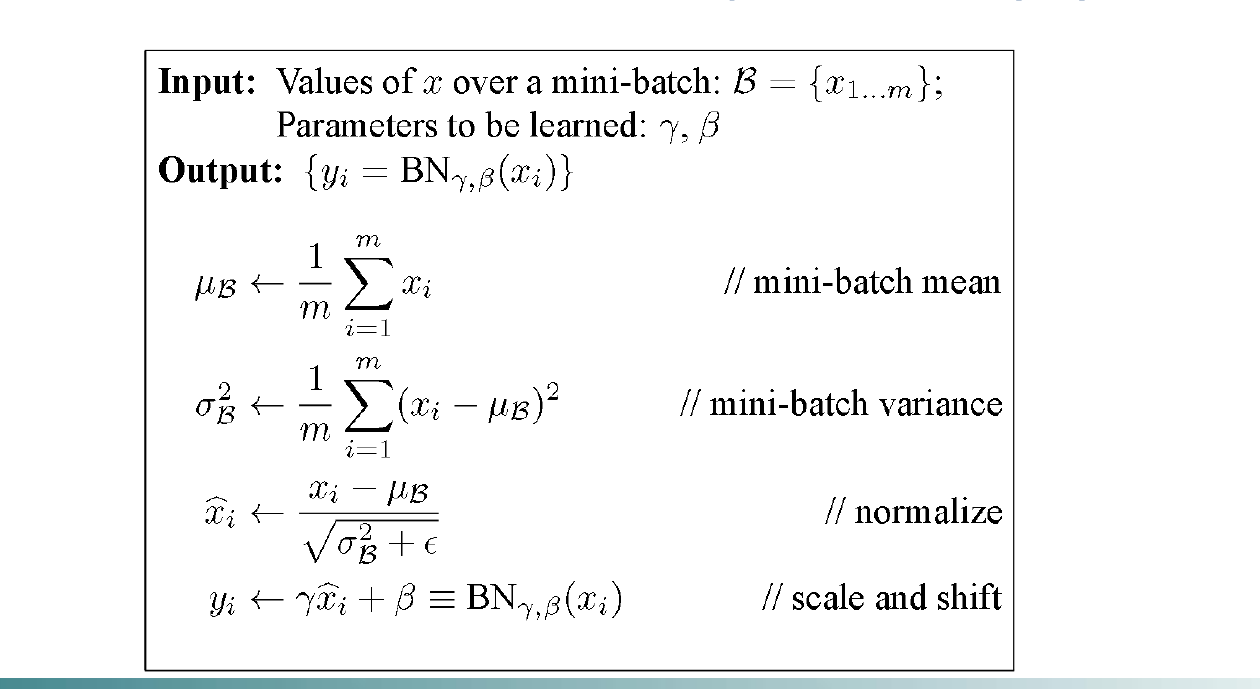
\includegraphics[width=0.62\linewidth]{figures/cf06_bn_algorithm.png}
  \caption{Pseudocodice dell'algoritmo di Batch Normalization come presentato
           nel paper originale \citep{ioffe2015batch}. Le quattro operazioni
           (media, varianza, normalizzazione, scale-and-shift) costituiscono
           il forward pass del layer BN.}
  \label{fig:bn_algorithm}
\end{figure}

\subsection{Parametri Apprendibili $\gamma$ e $\beta$}
\label{subsec:bn-gamma-beta}

Senza $\gamma$ e $\beta$, l'output del layer BN avrebbe sempre media $0$ e
deviazione standard $1$, limitando la capacità rappresentativa della rete.
I parametri $\gamma$ (fattore di scala) e $\beta$ (bias) permettono alla rete
di operare su qualsiasi range di valori.

Un aspetto cruciale è che $\gamma$ e $\beta$ \textbf{non annullano la
normalizzazione}: sono parametri appresi per discesa del gradiente e risultano
molto più stabili di $\mu$ e $\sigma$ (che cambiano ad ogni mini-batch). Il
layer ha persino la capacità di imparare la funzione identità (per
``de-normalizzare'' se necessario), ma lo fa solo se il task lo richiede.

%------------------------------------------------------------
\section{Vantaggi della Batch Normalization}
\label{sec:bn-benefits}

\subsection{Benefici Teorici (Motivazione Originale)}
\label{subsec:bn-theory}

\begin{description}
  \item[Riduzione dell'Internal Covariate Shift] La motivazione originale
        del paper. Con BN, ogni neurone tende ad avere un'attivazione
        approssimativamente gaussiana (solitamente non attivo, a volte
        parzialmente attivo, raramente molto attivo). Il covariate shift è
        indesiderabile perché i layer successivi devono continuamente
        adattarsi a cambiamenti nel \emph{tipo} di distribuzione, non solo
        nei parametri.

        \begin{tcolorbox}[colback=orange!5!white, colframe=orange!60!black,
                          title={Nota critica}]
          \textbf{Questa motivazione è stata confutata sperimentalmente.}
          Ricerche successive hanno dimostrato che BN non riduce
          significativamente l'internal covariate shift. I veri benefici
          hanno spiegazioni diverse (cfr.\ Sezione~\ref{sec:why-works}).
        \end{tcolorbox}

  \item[Riduzione di vanishing/exploding gradients] Con attivazioni
        distribuite normalmente, il segnale del gradiente si propaga in modo
        più stabile tra i layer. Senza BN, attivazioni basse in un layer
        possono propagarsi a cascata producendo attivazioni sempre più piccole
        nei layer successivi.
\end{description}

\subsection{Benefici Pratici}
\label{subsec:bn-practical}

\begin{itemize}
  \item \textbf{Riduce i tempi di training}: meno problemi di gradienti
        anomali $\Rightarrow$ convergenza più rapida.
  \item \textbf{Riduce il bisogno di regolarizzazione} (dropout, L2): le
        medie e varianze calcolate sul batch introducono rumore stocastico
        che impedisce alla rete di memorizzare le risposte corrette per ogni
        esempio (effetto implicito di regolarizzazione).
  \item \textbf{Permette learning rate più alti}: minor pericolo di
        esplosione del gradiente consente di usare $\eta$ più grandi senza
        instabilità.
  \item \textbf{Abilita funzioni di attivazione saturanti in reti profonde}:
        la normalizzazione impedisce alle attivazioni di finire nelle zone di
        saturazione della sigmoide (valori molto alti o molto bassi), dove
        il gradiente è quasi nullo.
\end{itemize}

\begin{figure}[H]
  \centering
  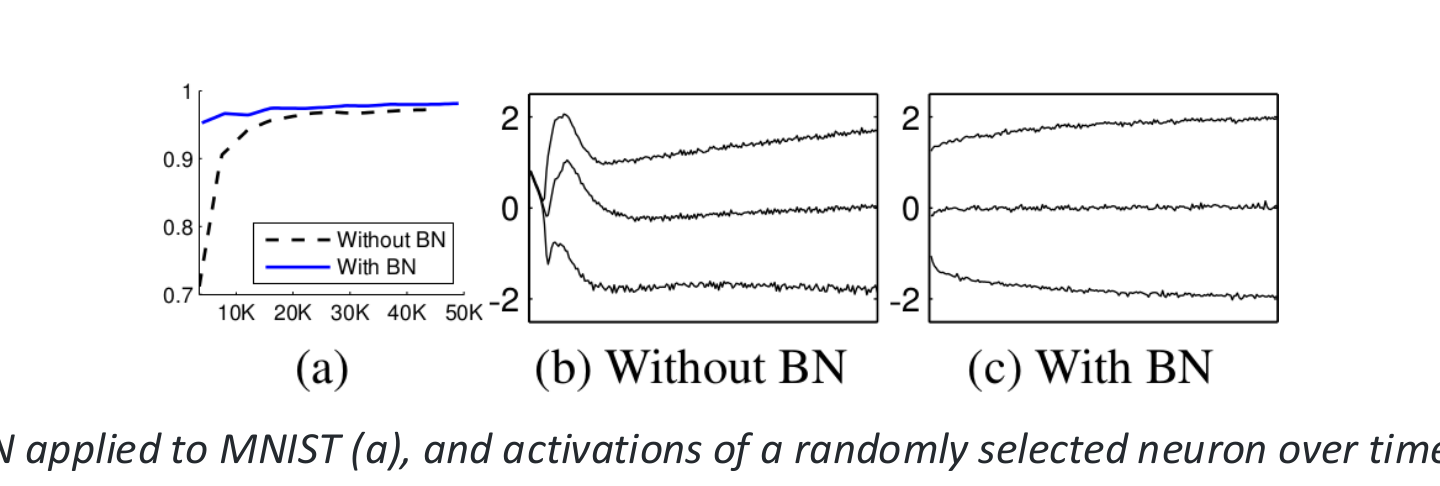
\includegraphics[width=0.82\linewidth]{figures/cf06_bn_mnist_activations.png}
  \caption{Risultati sperimentali su MNIST \citep{ioffe2015batch}.
           (a) Accuratezza durante il training: con BN si raggiunge
           convergenza più rapida e accuratezza finale più alta.
           (b) Senza BN: l'attivazione di un neurone casuale oscilla
           ampiamente nel tempo. (c) Con BN: le attivazioni si stabilizzano
           presto e rimangono nella stessa distribuzione per tutto il
           training.}
  \label{fig:bn_mnist}
\end{figure}

%------------------------------------------------------------
\section{Posizionamento del Layer BN}
\label{sec:bn-position}

Il BN layer viene tipicamente inserito \textbf{tra il layer lineare (o
convolutivo) e la funzione di attivazione}. Questa posizione permette di
normalizzare le attivazioni prima che vengano passate alla non-linearità,
evitando la saturazione.

\begin{figure}[H]
  \centering
  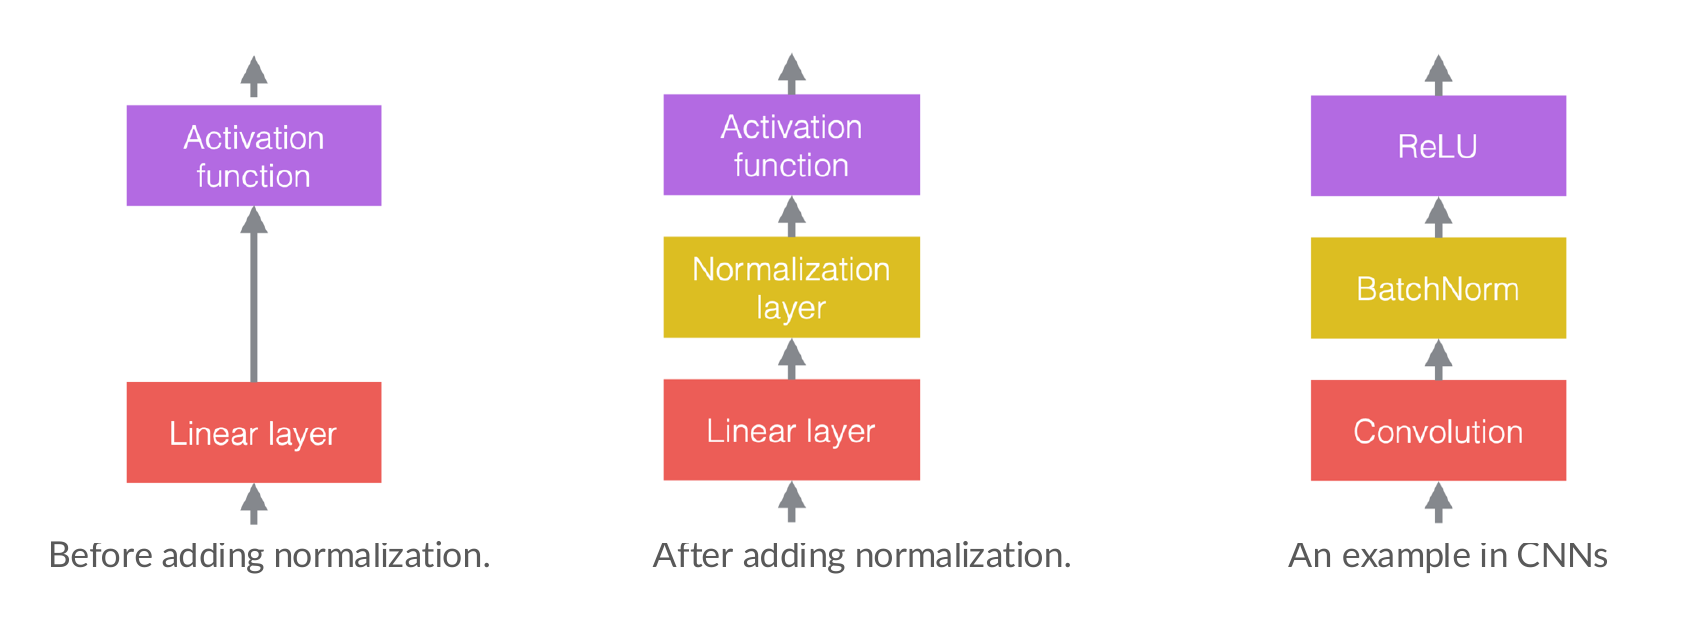
\includegraphics[width=0.82\linewidth]{figures/cf06_bn_positions.png}
  \caption{Posizionamento del layer di normalizzazione nell'architettura.
           Sinistra: rete senza normalizzazione (Linear $\to$ Activation).
           Centro: rete con normalizzazione (Linear $\to$ Norm $\to$
           Activation). Destra: esempio tipico in una CNN (Convolution $\to$
           BatchNorm $\to$ ReLU).}
  \label{fig:bn_positions}
\end{figure}

\paragraph{Fase di inferenza.}
Durante il training, $\mu$ e $\sigma^2$ vengono calcolati sul mini-batch
corrente. Durante l'inferenza, non si può usare lo stesso approccio
(il batch potrebbe contenere un solo esempio). Si usano invece le
\textbf{statistiche mobili} (running mean e running variance) accumulate
durante il training:

\begin{equation}
  \hat{\mu} \leftarrow (1 - \alpha)\,\hat{\mu} + \alpha\,\mu_{\mathcal{B}},
  \qquad
  \hat{\sigma}^2 \leftarrow (1 - \alpha)\,\hat{\sigma}^2
                             + \alpha\,\sigma_{\mathcal{B}}^2.
\end{equation}

In PyTorch questo comportamento è gestito automaticamente con
\texttt{model.train()} e \texttt{model.eval()}.

%------------------------------------------------------------
\section{Varianti di Normalizzazione}
\label{sec:norm-variants}

La scelta di \emph{quali} elementi del tensore usare per calcolare media e
varianza dà origine a diverse varianti. Per un mini-batch di $N$ immagini di
altezza $H$, larghezza $W$ e $C$ canali:

\begin{figure}[H]
  \centering
  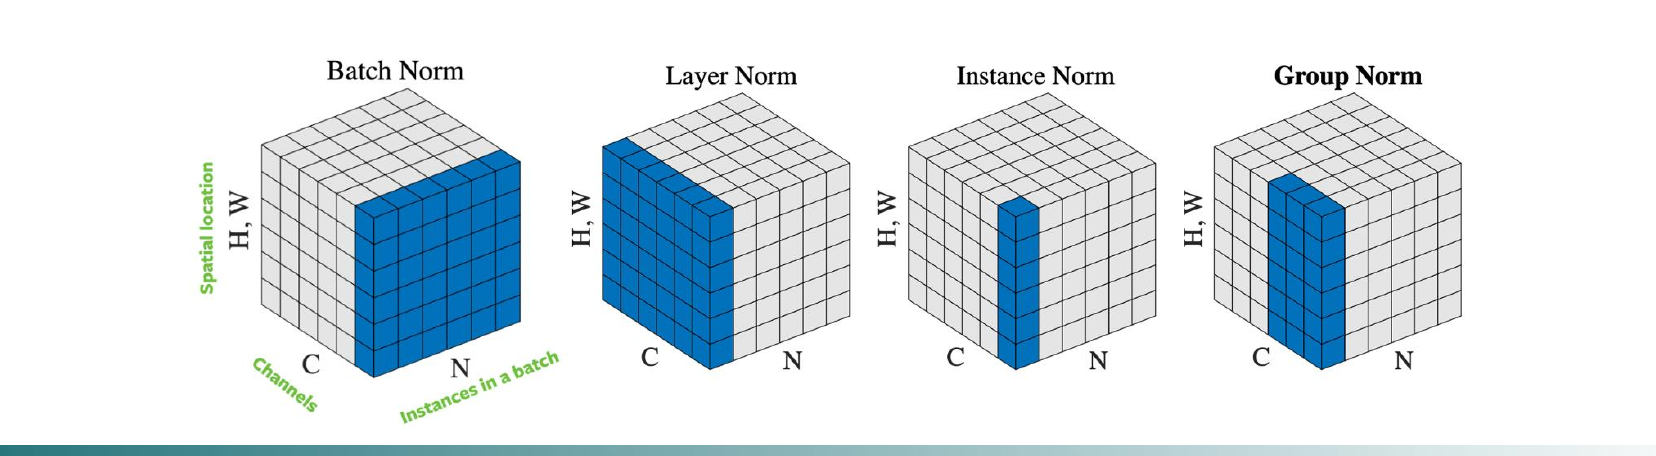
\includegraphics[width=0.90\linewidth]{figures/cf06_norm_types.png}
  \caption{Le quattro principali operazioni di normalizzazione. In blu sono
           evidenziati gli elementi usati per calcolare media e varianza per
           ogni singola statistica. Assi: $N$ (istanze nel batch), $C$
           (canali), $H \times W$ (posizioni spaziali).}
  \label{fig:norm_types}
\end{figure}

\subsection{Batch Normalization (BN)}
\label{subsec:bn-variant}

Normalizza \textbf{lungo la dimensione del batch} $N$: per ogni canale $c$,
calcola media e varianza su tutti gli elementi $(n, c, h, w)$ al variare di
$n$, $h$, $w$. Produce statistiche stabili per batch grandi ma è inadatta a
batch piccoli (le stime di $\mu$ e $\sigma$ diventano rumorose) o a sequenze
di lunghezza variabile.

\begin{equation}
  \mu_c = \frac{1}{N \cdot H \cdot W} \sum_{n,h,w} x_{n,c,h,w}, \qquad
  \sigma_c^2 = \frac{1}{N \cdot H \cdot W}
               \sum_{n,h,w} (x_{n,c,h,w} - \mu_c)^2.
\end{equation}

\subsection{Layer Normalization (LN)}
\label{subsec:layer-norm}

Normalizza \textbf{lungo i canali} per ogni singola istanza: per ogni
campione $n$, calcola media e varianza su tutti i canali e le posizioni
spaziali. Non dipende dal batch, quindi funziona perfettamente con batch di
dimensione $1$ ed è la scelta standard nei \textbf{Transformer} (dove le
sequenze hanno lunghezza variabile).

\begin{equation}
  \mu_n = \frac{1}{C \cdot H \cdot W} \sum_{c,h,w} x_{n,c,h,w}.
\end{equation}

In PyTorch: \texttt{nn.LayerNorm}.

\subsection{Instance Normalization (IN)}
\label{subsec:instance-norm}

Normalizza \textbf{per canale per istanza}: media e varianza sono calcolate
su $H \times W$ per ogni coppia $(n, c)$ indipendentemente. Utile in
\textbf{style transfer} e generazione di immagini, dove la normalizzazione
deve essere specifica per ogni immagine e ogni feature map.

\begin{equation}
  \mu_{n,c} = \frac{1}{H \cdot W} \sum_{h,w} x_{n,c,h,w}.
\end{equation}

In PyTorch: \texttt{nn.InstanceNorm2d}.

\subsection{Group Normalization (GN)}
\label{subsec:group-norm}

Compromesso tra LN e IN: divide i $C$ canali in $G$ gruppi e normalizza
ogni gruppo separatamente per ogni istanza. Non dipende da $N$ e mantiene
buone prestazioni anche con batch piccoli (es.\ $N=1$ o $N=2$ tipici in
object detection con immagini ad alta risoluzione).

\begin{equation}
  \mu_{n,g} = \frac{1}{(C/G) \cdot H \cdot W}
               \sum_{c \in \text{gruppo } g, h, w} x_{n,c,h,w}.
\end{equation}

In PyTorch: \texttt{nn.GroupNorm}. Con $G = C$ si ottiene Instance Norm;
con $G = 1$ si ottiene Layer Norm.

\begin{table}[H]
  \centering
  \caption{Confronto delle varianti di normalizzazione.}
  \label{tab:norm_comparison}
  \small
  \begin{tabular}{lllll}
    \toprule
    \textbf{Metodo} & \textbf{Calcola su} & \textbf{Dipende da $N$?}
      & \textbf{Uso tipico} & \textbf{PyTorch} \\
    \midrule
    Batch Norm   & $N, H, W$ per canale  & Sì  & CNN classifica  & \texttt{BatchNorm2d} \\
    Layer Norm   & $C, H, W$ per istanza & No  & Transformer, RNN & \texttt{LayerNorm} \\
    Instance Norm & $H, W$ per (n,c)     & No  & Style transfer  & \texttt{InstanceNorm2d} \\
    Group Norm   & gruppo di canali per istanza & No & Detection, segm. & \texttt{GroupNorm} \\
    \bottomrule
  \end{tabular}
\end{table}

%------------------------------------------------------------
\section{Perché la Normalizzazione Funziona Davvero?}
\label{sec:why-works}

Nonostante la normalizzazione funzioni bene in pratica, le ragioni della sua
efficacia sono ancora oggetto di dibattito. La motivazione originale
(riduzione dell'internal covariate shift) è stata confutata sperimentalmente.
I meccanismi attualmente più accreditati sono tre:

\begin{description}
  \item[Effetto di ottimizzazione] Le reti con layer di normalizzazione sono
        più facili da ottimizzare e permettono l'uso di learning rate più
        alti. La normalizzazione \emph{liscia} la superficie di perdita,
        rendendola più uniforme e riducendo la necessità di seguire
        direzioni di gradiente complesse.

  \item[Effetto di regolarizzazione] Le stime di media e varianza calcolate
        su un mini-batch sono \textbf{rumorose} (cambiano da batch a batch).
        Questo rumore aggiuntivo agisce come un regolarizzatore implicito,
        migliorando la generalizzazione in modo simile al dropout. La rete
        non può memorizzare valori fissi perché la normalizzazione li cambia
        ad ogni step.

  \item[Riduzione della sensibilità all'inizializzazione dei pesi] Grazie
        alla normalizzazione, l'inizializzazione dei pesi diventa meno
        critica: la distribuzione delle attivazioni viene corretta
        automaticamente al primo forward pass.
\end{description}

Come conseguenza pratica, la normalizzazione permette di essere più
``distratti'' nella progettazione: si possono combinare quasi qualsiasi
blocco architetturale e avere buone probabilità di convergenza senza dover
analizzare il condizionamento della rete.

%------------------------------------------------------------
\section{Riepilogo e Linee Guida Pratiche}
\label{sec:norm-summary}

\paragraph{Regole operative.}
\begin{enumerate}
  \item Per \textbf{CNN su immagini con batch $\geq 16$}: usare
        \texttt{nn.BatchNorm2d} dopo ogni layer conv, prima della ReLU.
        Ricordare di chiamare \texttt{model.eval()} durante l'inferenza per
        usare le running statistics.
  \item Per \textbf{Transformer e modelli sequence-to-sequence}: usare
        \texttt{nn.LayerNorm}; BN è inadatta a sequenze di lunghezza
        variabile e batch piccoli.
  \item Per \textbf{object detection / segmentazione semantica} con batch
        piccoli ($N \leq 4$): preferire \texttt{nn.GroupNorm} (tipicamente
        $G = 32$) che non degrada al calare di $N$.
  \item Per \textbf{style transfer e GAN}: \texttt{nn.InstanceNorm2d}
        normalizza per immagine, preservando le statistiche di stile
        specifiche per ciascun esempio.
  \item Non usare BN dopo layer con batch size $1$ o in presenza di
        sequenze molto corte: le stime di $\mu$ e $\sigma$ saranno
        inaffidabili.
  \item Ricordarsi che BN introduce un bias implicito per ciascun canale
        tramite $\beta$: quando BN segue un layer lineare/conv con bias, il
        bias del layer precedente è ridondante e può essere disabilitato
        (\texttt{bias=False}).
\end{enumerate}

Come sottolinea \citet{bishop2024}, i layer di normalizzazione sono oggi
parte integrante di quasi ogni architettura di successo. La loro semplicità
implementativa, unita all'impatto significativo su velocità di convergenza e
generalizzazione, li rende uno strumento imprescindibile nel toolkit del Deep
Learning moderno.

%============================================================
%  Capitolo 7 – Reti Neurali Convoluzionali (CNN)
%============================================================
\chapter{Reti Neurali Convoluzionali}
\label{ch:cnn}

Le \textbf{Reti Neurali Convoluzionali} (Convolutional Neural Networks, CNN o ConvNet) sono
una classe di architetture progettate specificamente per elaborare dati strutturati su una
griglia, come le immagini (griglia 2D di pixel). La loro idea fondamentale risale ai lavori di
Fukushima sulla gerarchia semplice/complessa della corteccia visiva e alla prima CNN sviluppata
da Yann LeCun a Toronto tra il 1988 e il 1989, successivamente consolidata nel celebre lavoro
su LeNet-5 per il riconoscimento di cifre scritte a mano \citep{bishop2024}.

%------------------------------------------------------------
\section{Limiti delle Reti Completamente Connesse sulle Immagini}
\label{sec:fc-limits}

Nelle reti \emph{fully connected} classiche, ogni neurone riceve in ingresso tutti i valori del
volume di input. Questo approccio \textbf{non scala} alle immagini reali:

\begin{itemize}
  \item Un'immagine CIFAR-10 di dimensioni $32 \times 32 \times 3$ genera già
        $32 \cdot 32 \cdot 3 = 3072$ pesi per un singolo neurone del primo strato nascosto.
  \item Un'immagine di dimensioni più realistiche, ad esempio $200 \times 200 \times 3$,
        porterebbe a $200 \cdot 200 \cdot 3 = 120\,000$ pesi per neurone.
  \item Con molti neuroni i parametri si accumulano rapidamente, determinando
        \textbf{overfitting} e un costo computazionale proibitivo.
\end{itemize}

La connettività totale è dunque uno spreco: pixel vicini sono altamente correlati, e le feature
visive utili (bordi, texture, forme) compaiono in posizioni diverse dell'immagine ma con la
stessa struttura locale.

%------------------------------------------------------------
\section{Volumi 3D e Connettività Locale}
\label{sec:3d-volumes}

\subsection{Organizzazione tridimensionale}
\label{subsec:3d-org}

A differenza di una rete fully connected, i layer di una ConvNet organizzano le proprie unità
in \textbf{tre dimensioni}: larghezza ($W$), altezza ($H$) e profondità ($D$). Il termine
\emph{profondità} qui si riferisce alla terza dimensione del \emph{volume di attivazione} (per
esempio i 3 canali RGB di un'immagine), \emph{non} al numero di layer della rete.

\subsection{Connettività locale}
\label{subsec:local-connectivity}

Per input ad alta dimensionalità è impraticabile collegare ogni unità a tutti i valori del
volume precedente. La soluzione è connettere ogni unità soltanto a una \textbf{regione locale}
dell'input. L'estensione spaziale di questa connessione è un iperparametro chiamato
\textbf{campo recettivo} (receptive field) dell'unità, che coincide con la dimensione del
filtro.

Due proprietà fondamentali:
\begin{enumerate}
  \item \textbf{Connessione locale in 2D}: lungo larghezza e altezza ogni unità vede solo una
        piccola finestra dell'input.
  \item \textbf{Connessione piena in profondità}: lungo la dimensione di profondità la
        connessione si estende all'intera profondità del volume di input (ad esempio tutti e 3
        i canali RGB).
\end{enumerate}

%------------------------------------------------------------
\section{Il Layer di Convoluzione}
\label{sec:conv-layer}

\subsection{Operazione di convoluzione}
\label{subsec:conv-operation}

Il layer convoluzionale fa scorrere (\emph{slide}) un filtro $\mathbf{w}$ di dimensioni
$F \times F \times D$ su tutte le posizioni spaziali del volume di input. In ogni posizione
viene calcolato un \textbf{prodotto scalare} tra il filtro e il corrispondente blocco
dell'input, producendo un singolo scalare di attivazione:

\begin{equation}
  a = \mathbf{w}^{\top} \mathbf{x} + b,
  \label{eq:conv-dot}
\end{equation}

dove $\mathbf{x}$ è il vettore di $F \cdot F \cdot D$ valori del blocco corrente e $b$ è il
bias del filtro. Per un filtro $5 \times 5 \times 3$ il prodotto scalare ha dimensione
$5 \cdot 5 \cdot 3 = 75$.

\begin{figure}[H]
  \centering
  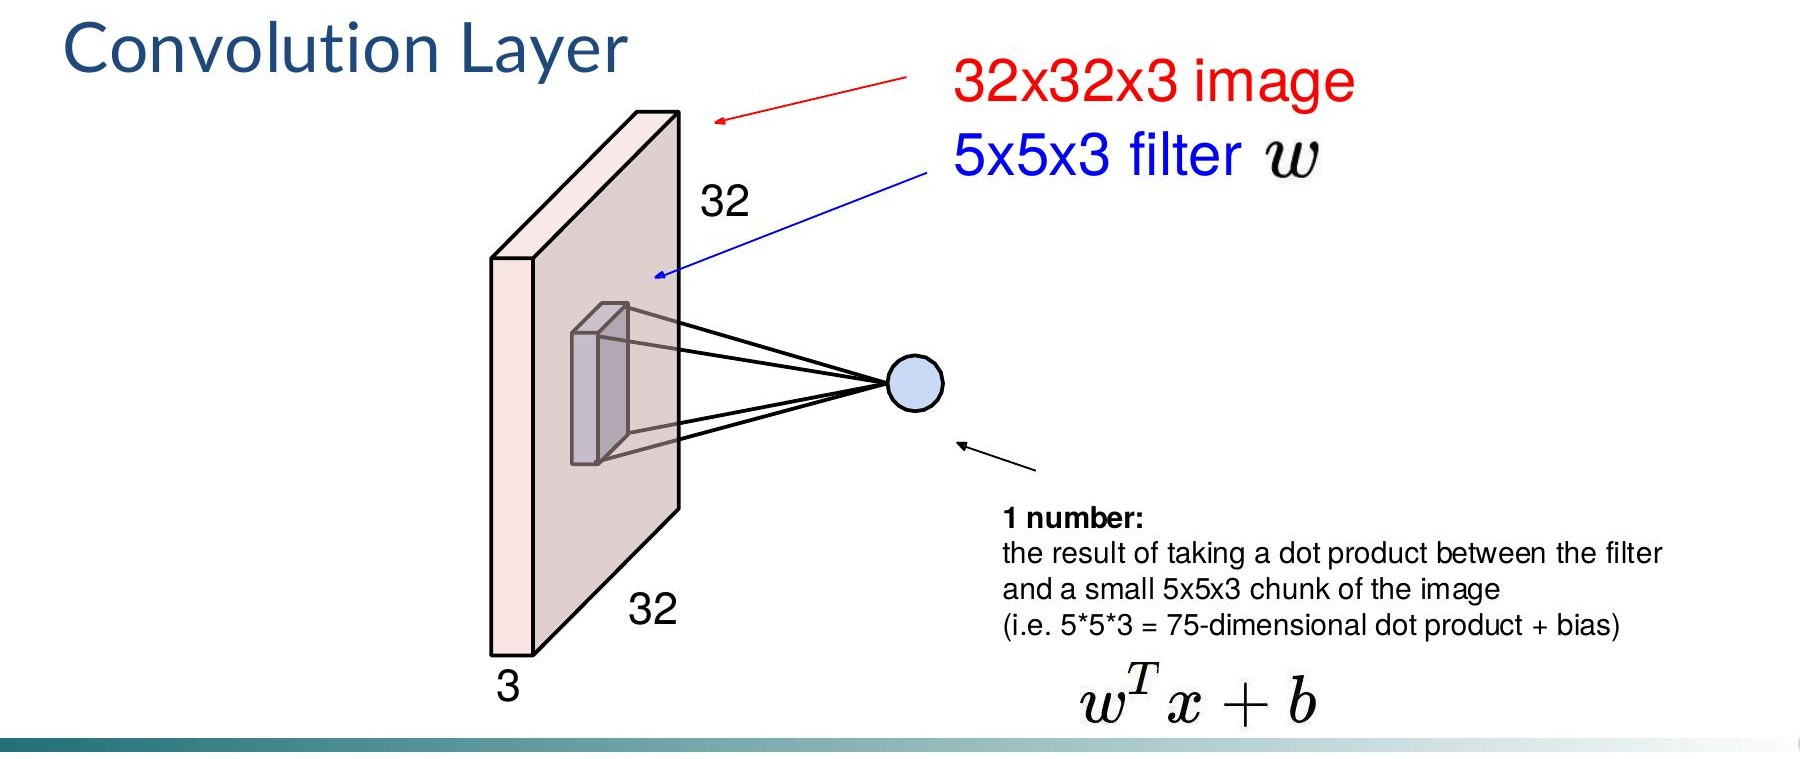
\includegraphics[width=0.82\linewidth]{figures/cf07_conv_dot_product.jpg}
  \caption{Convoluzione di un filtro $5\times5\times3$ su un'immagine $32\times32\times3$:
           ogni neurone di output calcola il prodotto scalare 75-dimensionale
           $\mathbf{w}^{\top}\mathbf{x}+b$ tra il filtro e il blocco locale dell'immagine.}
  \label{fig:conv-dot}
\end{figure}

Il layer si chiama \emph{convoluzionale} perché l'operazione è formalmente legata alla
convoluzione discreta tra due segnali:
\begin{equation}
  (f * g)[x, y] = \sum_{n_1=-\infty}^{+\infty} \sum_{n_2=-\infty}^{+\infty}
    f[n_1, n_2]\cdot g[x - n_1,\, y - n_2],
  \label{eq:conv-formula}
\end{equation}
ovvero una moltiplicazione elemento per elemento e somma tra il filtro e il segnale (immagine).

\subsection{Mappe di attivazione}
\label{subsec:activation-maps}

Facendo scorrere un singolo filtro su tutto il volume di input si ottiene una
\textbf{mappa di attivazione} (activation map) bidimensionale. Se si usano $K$ filtri si
ottengono $K$ mappe, che vengono impilate lungo la dimensione di profondità per formare il
volume di output.

\begin{figure}[H]
  \centering
  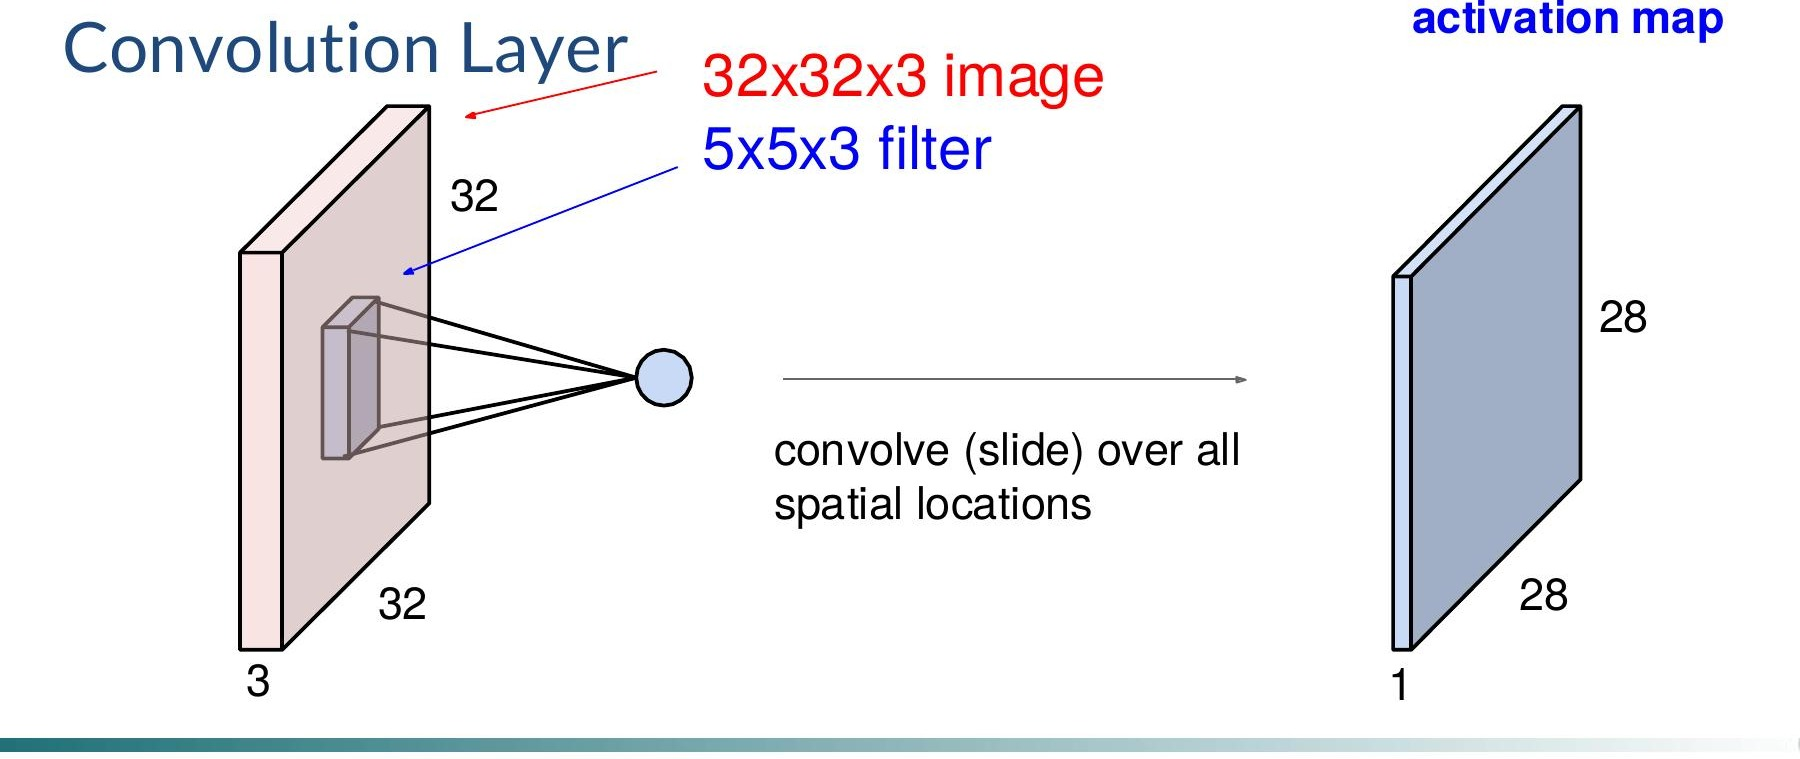
\includegraphics[width=0.82\linewidth]{figures/cf07_activation_map.jpg}
  \caption{Un singolo filtro $5\times5\times3$ applicato sull'immagine $32\times32\times3$
           produce una mappa di attivazione $28\times28\times1$.}
  \label{fig:activation-map}
\end{figure}

\begin{figure}[H]
  \centering
  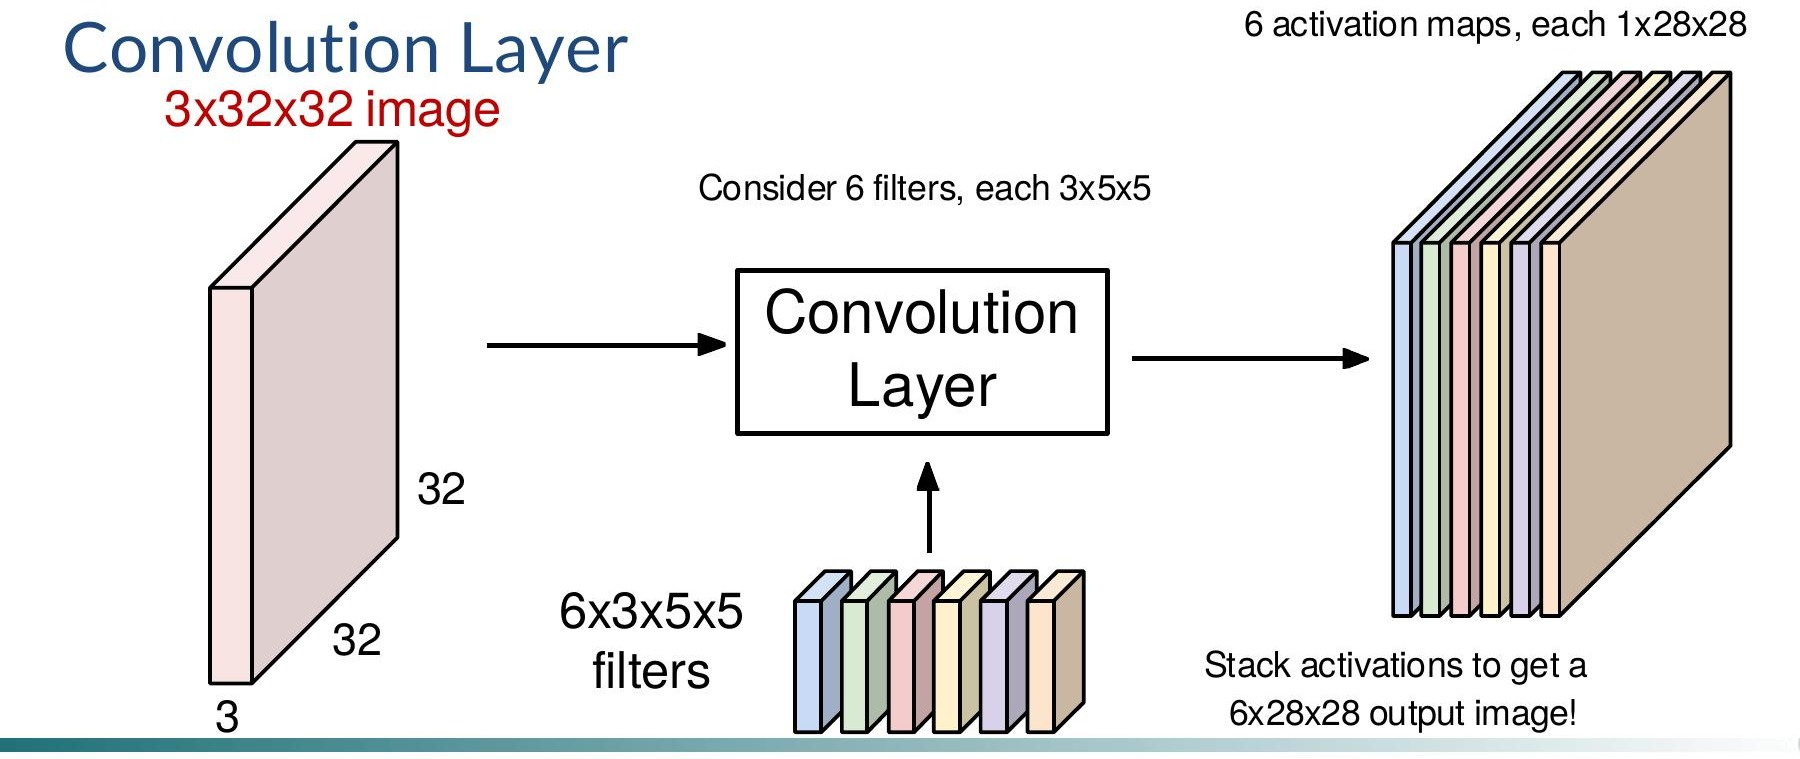
\includegraphics[width=0.90\linewidth]{figures/cf07_six_filters_output.jpg}
  \caption{Con 6 filtri $3\times5\times5$, il layer convoluzionale produce 6 mappe di
           attivazione che vengono impilate per ottenere un output $6\times28\times28$.}
  \label{fig:six-filters}
\end{figure}

\paragraph{Esempio.} Per un'immagine $32 \times 32 \times 3$ con un filtro $5 \times 5 \times
3$ e stride 1, la mappa di attivazione risultante ha dimensioni $28 \times 28 \times 1$. Con
6 filtri si ottiene un volume $28 \times 28 \times 6$.

In generale, con $K$ filtri di dimensione $F \times F \times D_{\text{in}}$:
\begin{itemize}
  \item ogni filtro ha $F \cdot F \cdot D_{\text{in}} + 1$ parametri (incluso il bias);
  \item il volume di output ha profondità $K$;
  \item il numero totale di parametri del layer è $K \cdot (F \cdot F \cdot D_{\text{in}} + 1)$.
\end{itemize}

\subsection{Dimensioni spaziali: stride e zero-padding}
\label{subsec:spatial-dims}

La dimensione spaziale dell'output dipende da tre iperparametri:

\begin{description}
  \item[Stride $S$] Passo con cui il filtro scorre sull'input. Stride maggiore produce output
        più piccoli e sottocampiona la rappresentazione.
  \item[Zero-padding $P$] Aggiunta di zeri intorno al bordo dell'input, che permette di
        controllare la dimensione dell'output.
  \item[Dimensione del filtro $F$] Controlla il campo recettivo locale.
\end{description}

La formula generale per la dimensione spaziale dell'output è:
\begin{equation}
  W_{\text{out}} = \frac{W_{\text{in}} + 2P - F}{S} + 1,
  \label{eq:output-size}
\end{equation}
e analogamente per $H_{\text{out}}$. Se il risultato non è intero, la combinazione
$(F, S, P)$ è incompatibile con l'input dato.

\begin{figure}[H]
  \centering
  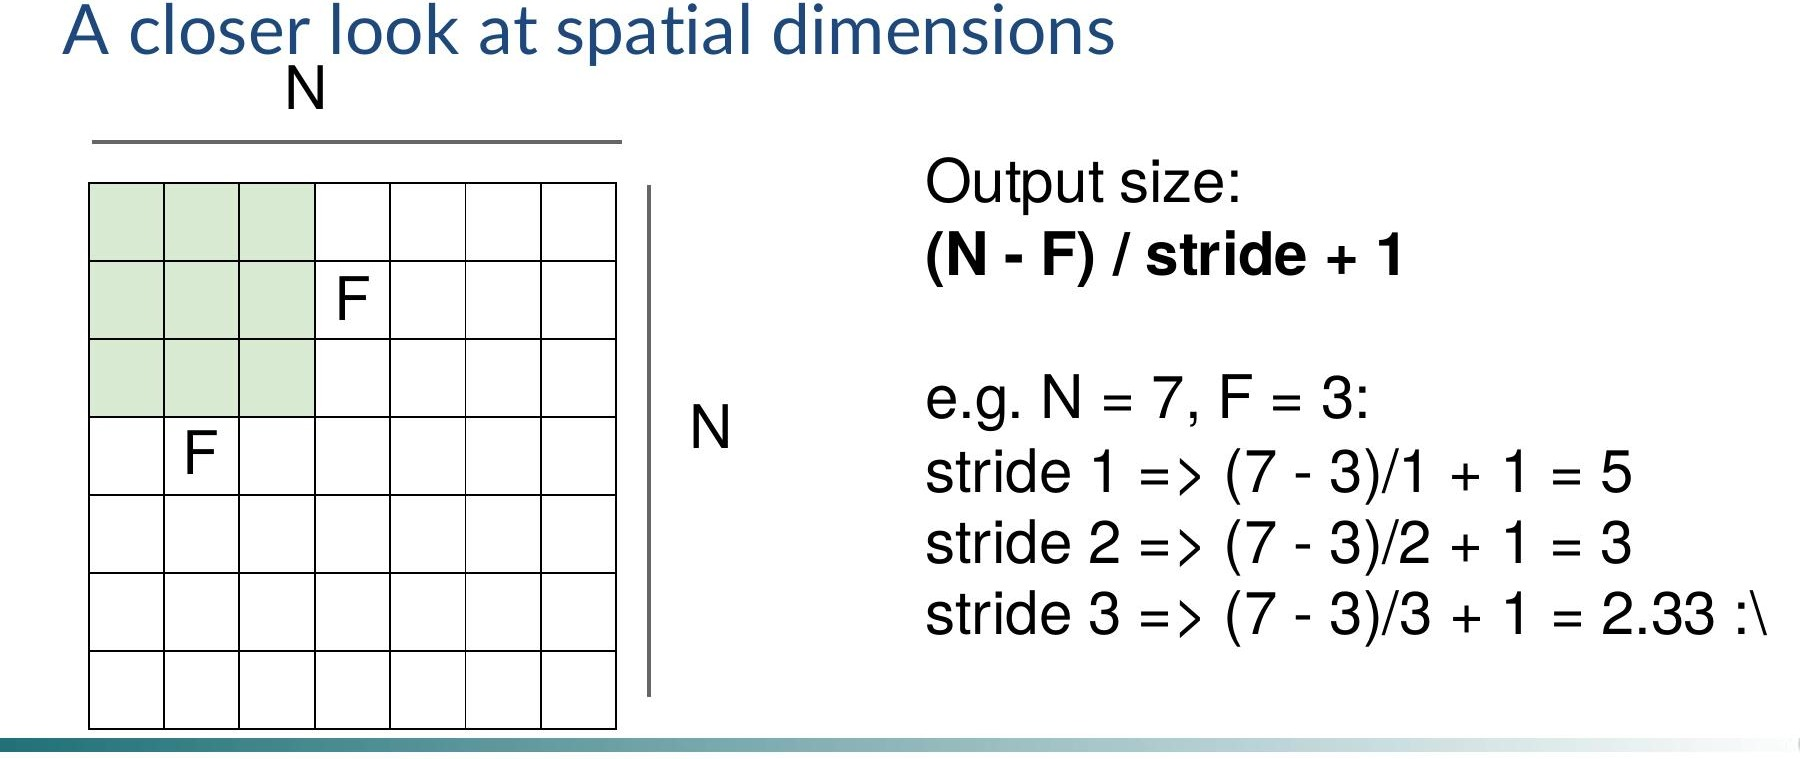
\includegraphics[width=0.82\linewidth]{figures/cf07_stride_formula.jpg}
  \caption{Formula per la dimensione dell'output $(N-F)/\text{stride}+1$ con esempi
           numerici: $N=7,\,F=3$ con stride 1 ($\to5$), stride 2 ($\to3$), stride 3
           (risultato non intero $\Rightarrow$ non valido).}
  \label{fig:stride-formula}
\end{figure}

\paragraph{Zero-padding per preservare la dimensione.} È comune usare stride 1, filtri di
dimensione $F \times F$ e zero-padding pari a $P = (F-1)/2$: questo preserva la dimensione
spaziale dell'input (formula aggiornata: $(N + 2P - F)/S + 1$). Per esempio,
$F = 3 \Rightarrow P = 1$; $F = 5 \Rightarrow P = 2$; $F = 7 \Rightarrow P = 3$.

\begin{figure}[H]
  \centering
  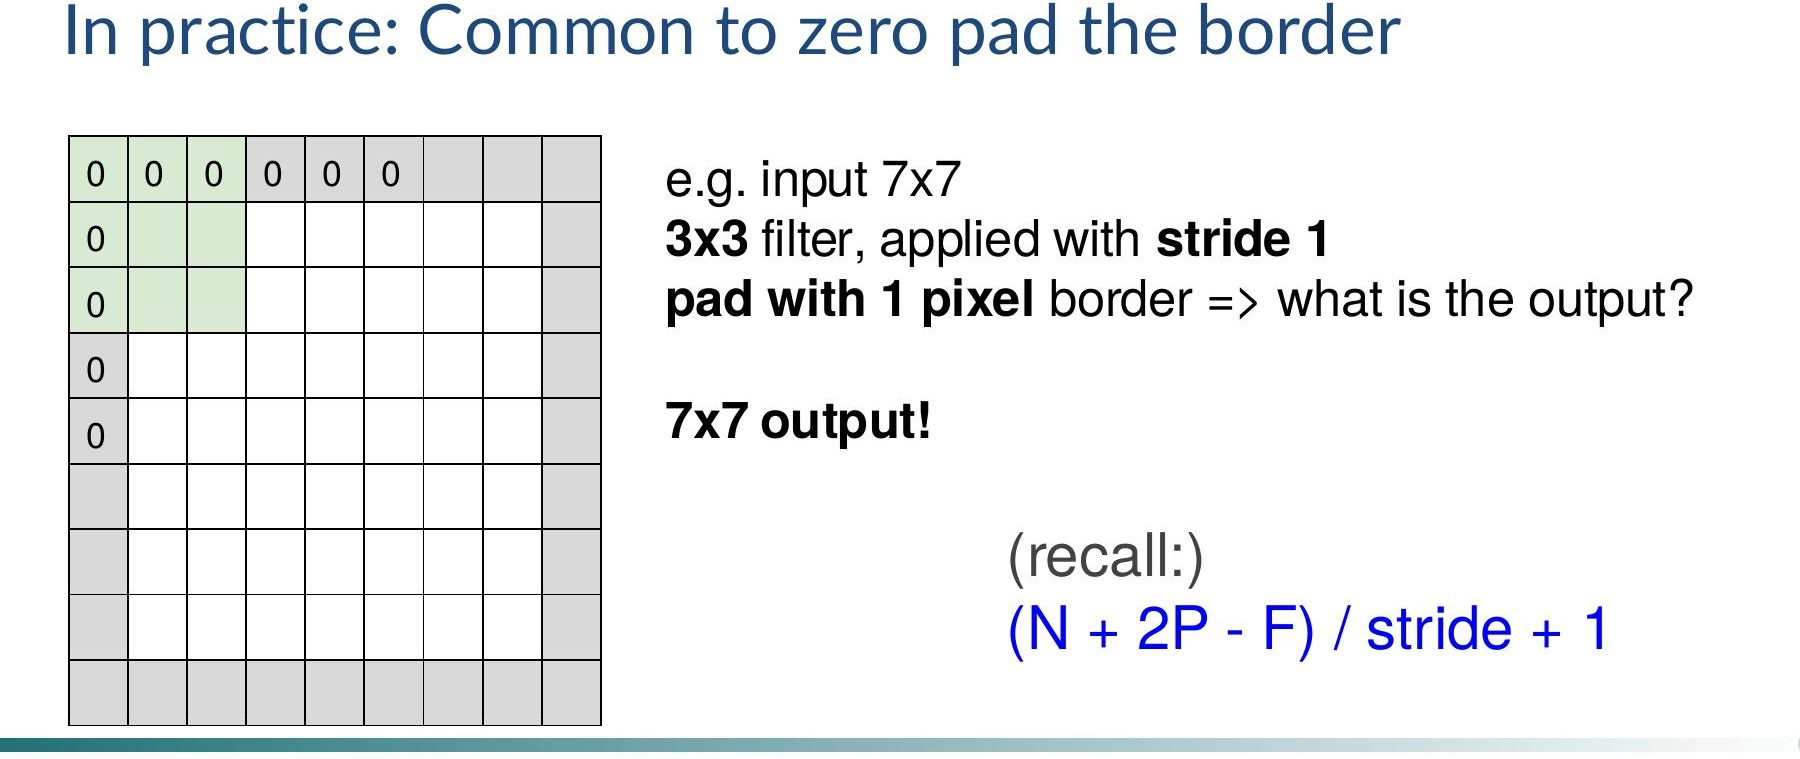
\includegraphics[width=0.82\linewidth]{figures/cf07_zero_padding.jpg}
  \caption{Zero-padding di 1 pixel intorno a un input $7\times7$: con filtro $3\times3$ e
           stride 1, l'output è ancora $7\times7$ (formula: $(7+2\cdot1-3)/1+1=7$).}
  \label{fig:zero-padding}
\end{figure}

\subsection{Convoluzione 1\texttimes1}
\label{subsec:1x1-conv}

Un filtro di dimensione $1 \times 1 \times D_{\text{in}}$ esegue un prodotto scalare
$D_{\text{in}}$-dimensionale in ogni posizione spaziale senza alcuna interazione spaziale.
Questo tipo di convoluzione è utile per:
\begin{itemize}
  \item \textbf{Riduzione di dimensionalità} lungo la profondità (collo di bottiglia),
        senza modificare la risoluzione spaziale.
  \item Aggiungere nonlinearità puntuali tra i layer convoluzionali.
\end{itemize}

%------------------------------------------------------------
\section{Campi Recettivi}
\label{sec:receptive-fields}

Il \textbf{campo recettivo} di un'unità è la regione dell'input originale che influenza il suo
valore di attivazione. Con un kernel di dimensione $K$, ogni elemento dell'output dipende da
una regione $K \times K$ del layer precedente. Ogni convoluzione successiva aggiunge $K-1$
alla dimensione del campo recettivo; con $L$ layer:

\begin{equation}
  \text{RF} = 1 + L \cdot (K - 1).
  \label{eq:receptive-field}
\end{equation}

\begin{figure}[H]
  \centering
  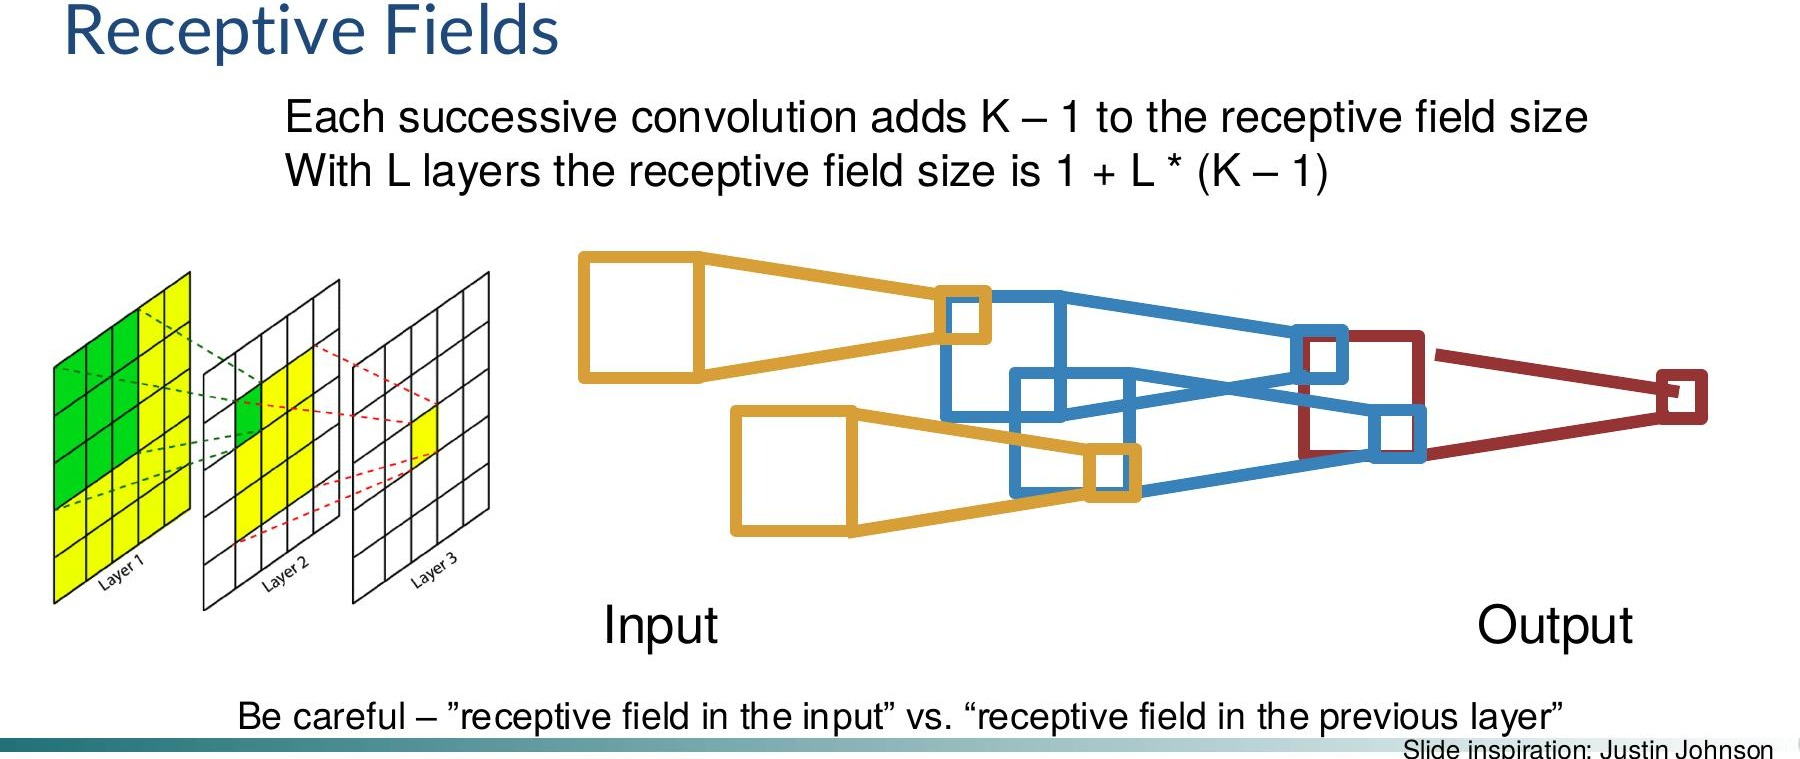
\includegraphics[width=0.88\linewidth]{figures/cf07_receptive_fields.jpg}
  \caption{Campi recettivi attraverso tre layer convoluzionali successivi: ogni layer
           espande la porzione dell'input originale vista da ciascuna unità. Con $L$ layer
           e kernel $K$, il campo recettivo totale sull'input è $1+L(K-1)$.
           Nota: ``receptive field in the input'' vs.\  ``receptive field in the previous
           layer'' sono concetti distinti.}
  \label{fig:receptive-fields}
\end{figure}

\paragraph{Problema per immagini grandi.}
Per immagini grandi è necessario un numero molto elevato di layer affinché ogni unità
dell'output ``veda'' l'intera immagine. La \textbf{soluzione} è il sottocampionamento
(\emph{downsampling}) all'interno della rete, ottenuto con:
\begin{itemize}
  \item \textbf{Convoluzione con stride $> 1$}: riduce direttamente la risoluzione spaziale.
  \item \textbf{Pooling}: layer dedicati al sottocampionamento (vedi
        Sezione~\ref{sec:pooling}).
\end{itemize}

%------------------------------------------------------------
\section{Cosa Imparano i Filtri Convoluzionali?}
\label{sec:what-filters-learn}

I filtri del primo layer fungono da \emph{template} locali sull'immagine. Dopo l'addestramento
su grandi dataset, i filtri del primo layer imparano a rilevare feature di basso livello come
bordi orientati in varie direzioni, colori opposti e frequenze spaziali diverse (in AlexNet,
64 filtri $3\times11\times11$). Nei layer successivi le mappe combinano le risposte precedenti,
rilevando pattern di complessità crescente: angoli al secondo layer, parti di oggetti al
terzo, interi oggetti agli strati più profondi.

%------------------------------------------------------------
\section{Il Layer di Pooling}
\label{sec:pooling}

Il layer di pooling serve a \textbf{ridurre la risoluzione spaziale} delle mappe di
attivazione, rendendo la rappresentazione più compatta e introducendo una certa
\textbf{invarianza traslazionale}. Opera in modo \emph{indipendente} su ciascuna mappa.

\subsection{Max Pooling}
\label{subsec:max-pooling}

Il \textbf{Max Pooling} è la variante più comune: data una finestra di dimensioni
$P_H \times P_W$ con stride $S$, si prende il massimo dei valori nella finestra.

\begin{figure}[H]
  \centering
  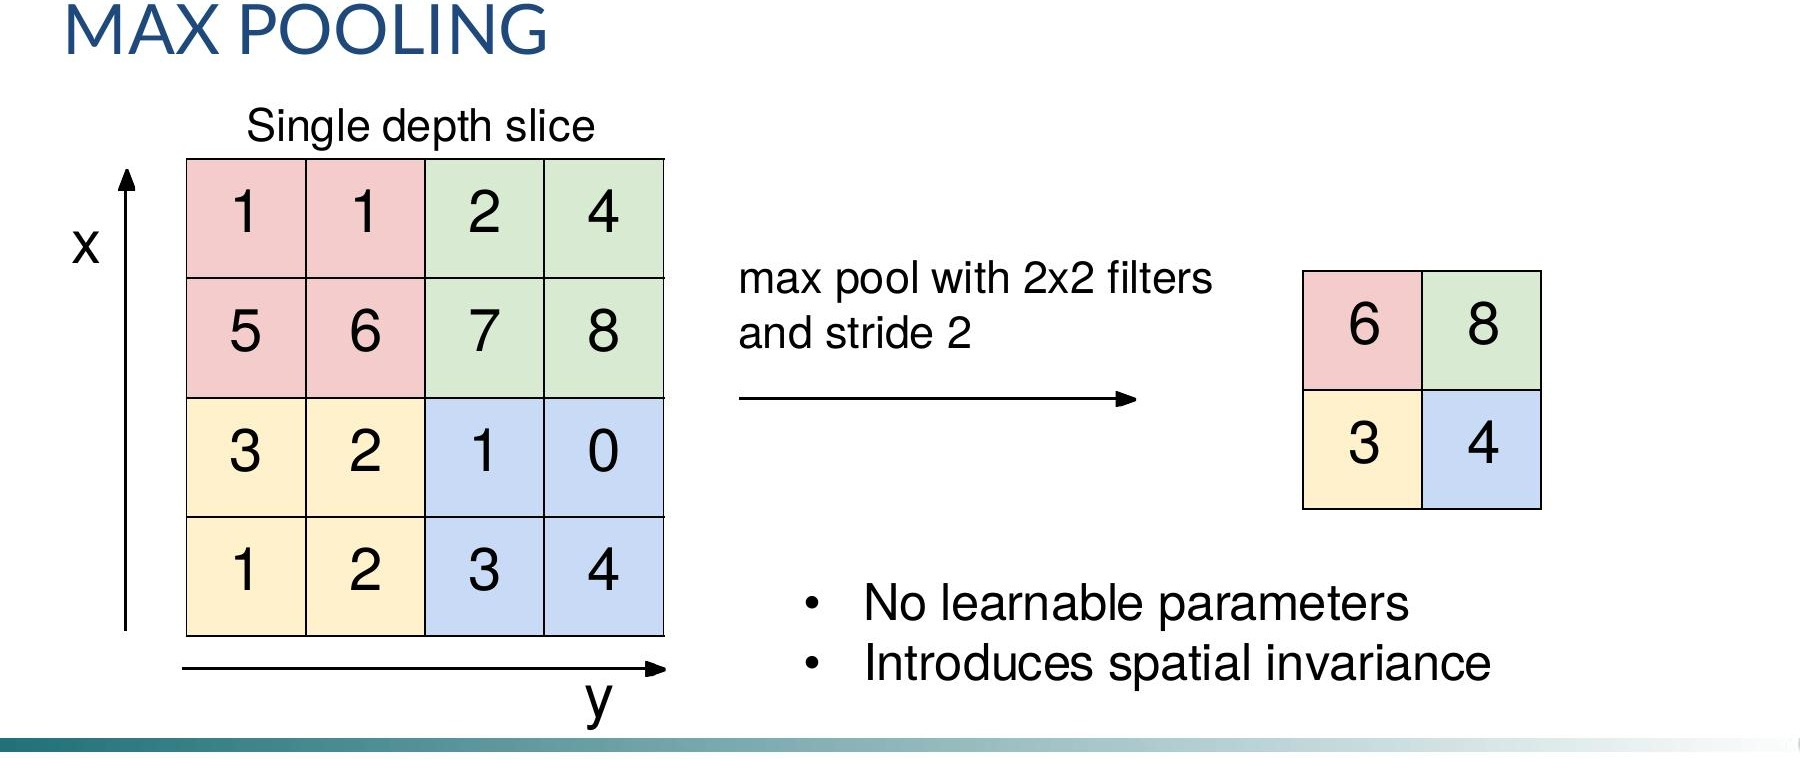
\includegraphics[width=0.82\linewidth]{figures/cf07_max_pooling.jpg}
  \caption{Max pooling $2\times2$ con stride 2 su una singola mappa $4\times4$: ogni
           quadrante $2\times2$ viene sostituito dal suo valore massimo, dimezzando la
           risoluzione spaziale. Nessun parametro apprendibile; introduce invarianza
           spaziale locale.}
  \label{fig:max-pooling}
\end{figure}

In formule, il max pooling $2\times2$ con stride 2 sull'esempio delle slide produce:
\begin{equation}
  \begin{pmatrix}
    1 & 1 & 2 & 4 \\
    5 & 6 & 7 & 8 \\
    3 & 2 & 1 & 0 \\
    1 & 2 & 3 & 4
  \end{pmatrix}
  \xrightarrow{\text{MaxPool }2\times2,\,s=2}
  \begin{pmatrix}
    6 & 8 \\
    3 & 4
  \end{pmatrix}.
  \label{eq:maxpool-example}
\end{equation}

Proprietà chiave: nessun parametro apprendibile; invarianza spaziale locale (piccole
traslazioni non cambiano l'output); riduzione spaziale tipicamente di un fattore 2.

\subsection{Altre varianti di pooling}
\label{subsec:other-pooling}

\begin{description}
  \item[Average Pooling] Calcola la media dei valori nella finestra.
  \item[Global Average Pooling (GAP)] Riduce ogni mappa a un unico scalare (media globale).
        Usato in GoogLeNet e ResNet come alternativa ai layer FC finali.
  \item[LP-Norm Pooling] $\bigl(\sum_i x_i^p\bigr)^{1/p}$; per $p\to\infty$ si ottiene il
        max pooling.
\end{description}

%------------------------------------------------------------
\section{Il Layer Fully Connected}
\label{sec:fc-layer}

Dopo un certo numero di layer CONV/ReLU/POOL, le mappe di attivazione vengono
\textbf{appiattite} (\emph{flatten}) in un vettore unidimensionale e passate a uno o più
\textbf{layer fully connected} (FC), dove ogni neurone è connesso a tutti i valori
dell'input. Questi layer eseguono la classificazione vera e propria combinando le feature
estratte dai layer convoluzionali. Il layer finale produce un punteggio per ciascuna delle
$C$ classi, tipicamente seguito da \textbf{softmax} per ottenere una distribuzione di
probabilità.

%------------------------------------------------------------
\section{Architettura Tipica di una ConvNet}
\label{sec:typical-arch}

Una ConvNet classica è costruita impilando ripetutamente layer CONV$+$ReLU, seguiti
periodicamente da layer di pooling e, alla fine, da layer FC:

\begin{equation}
  \underbrace{[(\text{CONV} \to \text{ReLU})^{\times N} \to \text{POOL?}]^{\times M}}
    _{\text{estrazione di feature}}
  \;\longrightarrow\;
  \underbrace{(\text{FC} \to \text{ReLU})^{\times K} \to \text{Softmax}}
    _{\text{classificazione}}
  \label{eq:typical-arch}
\end{equation}

dove tipicamente $N \lesssim 5$, $M$ è grande, $0 \le K \le 2$.

\paragraph{Trend moderni.}
\begin{itemize}
  \item Filtri piccoli ($3 \times 3$) in stack profondi al posto di filtri grandi (due
        $3\times3$ hanno lo stesso campo recettivo di un $5\times5$ ma con meno parametri e
        più nonlinearità).
  \item Eliminazione progressiva del pooling, sostituito da convoluzioni con stride 2.
  \item Architetture come \textbf{ResNet} e \textbf{GoogLeNet} sfidano il paradigma
        sequenziale con connessioni residue e moduli Inception.
\end{itemize}

\subsection{Esempio di stack convoluzionale}
\label{subsec:conv-stack-example}

\begin{table}[H]
  \centering
  \caption{Evoluzione delle dimensioni dei volumi in una ConvNet di esempio su
           un'immagine $32\times32\times3$.}
  \label{tab:conv-stack}
  \small
  \begin{tabular}{lccc}
    \toprule
    \textbf{Layer} & \textbf{Filtri / Operazione} & \textbf{Output} & \textbf{Param.} \\
    \midrule
    Input          & --                                       & $32\times32\times3$  & 0 \\
    CONV1+ReLU     & 6 filtri $5\times5$, $s=1$, $P=0$       & $28\times28\times6$  & 456 \\
    CONV2+ReLU     & 10 filtri $5\times5$, $s=1$, $P=0$      & $24\times24\times10$ & 1510 \\
    MaxPool        & $2\times2$, $s=2$                        & $12\times12\times10$ & 0 \\
    FC+ReLU        & 120 unità                                & $120$                & 173\,640 \\
    Softmax        & 10 classi                                & $10$                 & 1210 \\
    \bottomrule
  \end{tabular}
\end{table}

%------------------------------------------------------------
\section{Proprietà Fondamentali delle ConvNet}
\label{sec:cnn-properties}

\subsection{Parameter sharing}
\label{subsec:param-sharing}

In un layer convoluzionale, lo \textbf{stesso filtro} (con gli stessi pesi) viene applicato
in \emph{tutte} le posizioni spaziali dell'input. Questo si basa sull'assunzione che una
feature utile in una posizione sia utile anche in un'altra (\emph{equivarianza
traslazionale}). Il vantaggio pratico è una drastica riduzione del numero di parametri.

\subsection{Equivarianza traslazionale}
\label{subsec:equivariance}

La convoluzione è \textbf{equivariante per traslazione}: traslare l'input causa una
traslazione corrispondente nella mappa di attivazione. Formalmente, se $T_\Delta$ è una
traslazione di $\Delta$ posizioni:
\begin{equation}
  f(T_\Delta(\mathbf{x})) = T_\Delta(f(\mathbf{x})).
  \label{eq:equivariance}
\end{equation}
Il pooling con stride $> 1$ introduce invece \textbf{invarianza approssimata}: una
traslazione di 1 pixel nell'input diventa 0.5 pixel dopo un pooling $2\times2$.

\subsection{Connessioni sparse}
\label{subsec:sparse-conn}

Ogni unità dell'output dipende solo da una piccola regione locale dell'input invece che da
tutti i pixel, riducendo la complessità computazionale e favorendo la generalizzazione.

%------------------------------------------------------------
\section{Riepilogo dei Componenti Principali}
\label{sec:cnn-summary}

\begin{table}[H]
  \centering
  \caption{Riepilogo dei layer fondamentali di una ConvNet.}
  \label{tab:cnn-summary}
  \small
  \begin{tabular}{p{2.8cm}p{5.2cm}p{4.2cm}}
    \toprule
    \textbf{Layer} & \textbf{Funzione} & \textbf{Iperparametri principali} \\
    \midrule
    CONV            & Estrazione di feature locali tramite
                      prodotti scalari con filtri appresi &
                      $F$, $K$, $S$, $P$ \\
    \addlinespace
    ReLU            & Nonlinearità puntuale $\max(0,x)$ & -- \\
    \addlinespace
    POOL (Max/Avg)  & Sottocampionamento spaziale &
                      Finestra $P_H\times P_W$, $S$ \\
    \addlinespace
    FC              & Classificazione globale & Numero di unità \\
    \addlinespace
    Softmax         & Distribuzione di probabilità sulle classi & -- \\
    \bottomrule
  \end{tabular}
\end{table}

\paragraph{Regole pratiche.}
\begin{enumerate}
  \item Preferire filtri piccoli ($3 \times 3$) in stack profondi.
  \item Usare zero-padding $P = (F-1)/2$ per preservare la risoluzione nei layer CONV con
        stride 1.
  \item Il pooling $2 \times 2$ con stride 2 è la scelta più comune; il global average
        pooling è preferibile nei classificatori moderni.
  \item Verificare sempre che l'equazione~\eqref{eq:output-size} dia un intero.
  \item Aumentare la profondità (più filtri per layer) man mano che la risoluzione spaziale
        diminuisce, per mantenere la capacità rappresentativa della rete.
\end{enumerate}

Come sottolinea \citet{bishop2024}, la scelta dell'architettura convoluzionale è guidata da
considerazioni sul campo recettivo, dalla capacità del modello rispetto alla dimensione del
dataset e dal costo computazionale del training e dell'inference.

%============================================================
%  Capitolo 8 – Reti Ricorrenti
%============================================================
\chapter{Reti Ricorrenti}
\label{ch:recurrent-networks}

I dati del mondo reale sono spesso intrinsecamente \emph{sequenziali}: la
posizione futura di un oggetto in moto, le parole di un testo, le note di una
melodia o i fotogrammi di un video dipendono da ciò che è accaduto
\emph{prima}. Le reti neurali standard (feed-forward) ignorano questa struttura
temporale: ricevono un input di dimensione fissa e producono un output
indipendente da ogni elaborazione precedente. Le \textbf{reti neurali
ricorrenti} (RNN) colmano questa lacuna introducendo un meccanismo di
\emph{memoria implicita} che trasmette informazioni da un passo temporale al
successivo \citep{bishop2024}.

%------------------------------------------------------------
\section{Motivazione: Modellare Sequenze}
\label{sec:rnn-motivation}

\subsection{Il Problema della Modellazione Sequenziale}
\label{subsec:seq-problem}

Consideriamo il compito di predire la prossima parola in una frase. Un primo
approccio naïve consiste nell'usare una finestra fissa di $k$ parole precedenti
come input a una rete feed-forward (\emph{fixed-window approach}). Questo schema
soffre però di tre limitazioni fondamentali:

\begin{description}
  \item[Dipendenze a lungo termine] Una finestra fissa non può catturare
        contesti lontani nel tempo. Frase come \emph{``France is where I grew
        up, but I now live in Boston. I speak fluent \underline{\hspace{1cm}}''}
        richiedono informazioni che si trovano decine di parole prima.
  \item[Mancato rispetto dell'ordine] La rappresentazione a \emph{bag of words}
        codifica solo la presenza/assenza di parole: non distingue \emph{``The
        food was good, not bad at all''} da \emph{``The food was bad, not good
        at all''}.
  \item[Assenza di condivisione dei parametri] Con una finestra grande ogni
        posizione ha i propri pesi separati; ciò impedisce di trasferire le
        conoscenze apprese in una posizione alle altre.
\end{description}

Le RNN risolvono questi problemi mantenendo uno \textbf{stato nascosto}
$\mathbf{h}_t$ che riassume tutta la storia della sequenza fino al passo $t$.

\subsection{Rappresentazione Numerica del Linguaggio}
\label{subsec:word-embedding}

Le reti neurali richiedono input numerici; le parole devono essere quindi
trasformate in vettori. Il processo si articola in tre fasi: costruire un
\textbf{vocabolario} (corpus di tutte le parole), assegnare un indice a ogni
parola (\textbf{indicizzazione}), e infine convertire l'indice in un vettore di
dimensione fissa tramite \textbf{embedding}.

\begin{figure}[H]
  \centering
  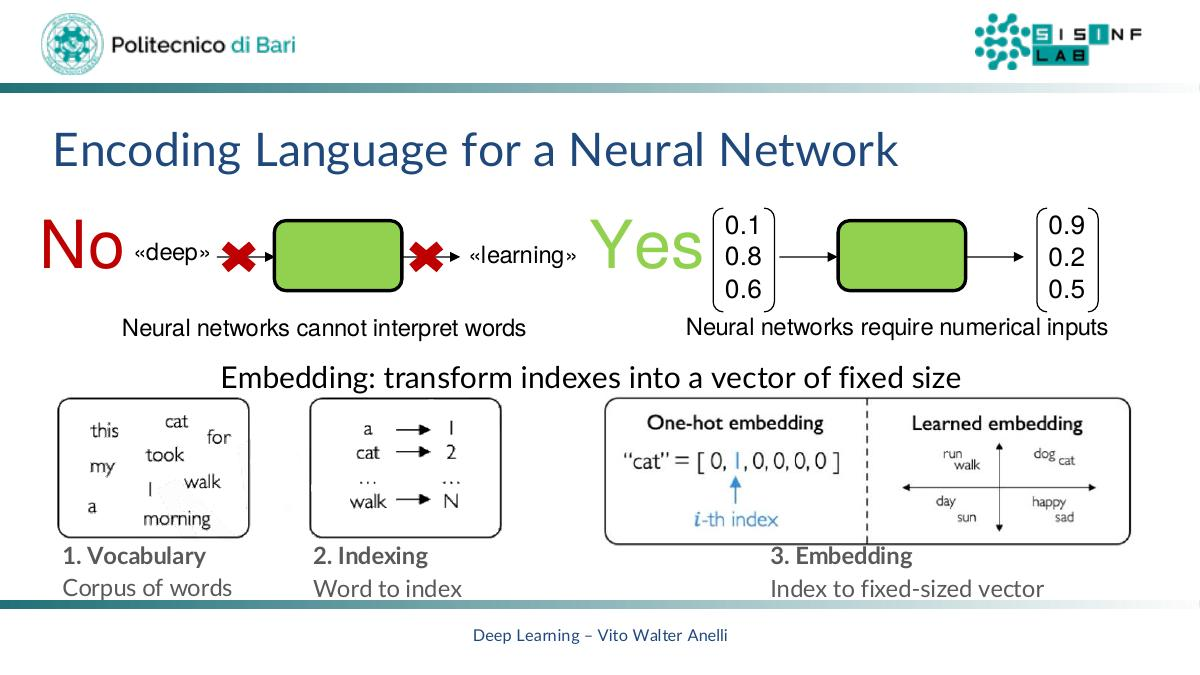
\includegraphics[width=0.82\linewidth]{figures/cf08_word_embedding.jpg}
  \caption{Codifica del linguaggio per una rete neurale. Sinistra: le parole non
           possono essere date direttamente in input. Centro: one-hot encoding
           (sparso, non apprende similarità semantiche). Destra: learned
           embedding (denso, cattura relazioni tra parole nello spazio
           vettoriale).}
  \label{fig:word_embedding}
\end{figure}

L'\textbf{one-hot encoding} rappresenta la parola $i$ come un vettore binario
di lunghezza $|V|$ con un solo 1 nella posizione $i$; è semplice ma non codifica
alcuna nozione di similarità semantica. Il \textbf{learned embedding} (es.
Word2Vec, GloVe) apprende durante l'addestramento una matrice
$E \in \mathbb{R}^{|V| \times d}$ che proietta ogni indice in un vettore denso
di dimensione $d$, catturando relazioni semantiche come
$\text{king} - \text{man} + \text{woman} \approx \text{queen}$.

%------------------------------------------------------------
\section{Reti Neurali Ricorrenti (RNN)}
\label{sec:rnn}

\subsection{Neuroni con Ricorrenza}
\label{subsec:neurons-recurrence}

Una rete feed-forward calcola $\hat{\mathbf{y}}_t = f(\mathbf{x}_t)$
indipendentemente per ogni passo temporale. Una \textbf{RNN} invece aggiunge
una connessione ricorrente dallo stato nascosto al passo precedente:

\begin{equation}
  \hat{\mathbf{y}}_t = f(\mathbf{x}_t,\, \mathbf{h}_{t-1}).
  \label{eq:rnn-output}
\end{equation}

L'equazione di \textbf{aggiornamento dello stato nascosto} e di
\textbf{produzione dell'output} di una RNN vanilla sono:

\begin{align}
  \mathbf{h}_t &= \tanh\!\left(W_{hh}^{T}\,\mathbf{h}_{t-1}
                   + W_{xh}^{T}\,\mathbf{x}_t\right),
  \label{eq:rnn-hidden} \\
  \hat{\mathbf{y}}_t &= W_{hy}^{T}\,\mathbf{h}_t,
  \label{eq:rnn-output2}
\end{align}

dove $W_{hh} \in \mathbb{R}^{d_h \times d_h}$, $W_{xh} \in \mathbb{R}^{d_x
\times d_h}$ e $W_{hy} \in \mathbb{R}^{d_h \times d_y}$ sono le matrici dei
pesi, \emph{condivise tra tutti i passi temporali}. Questa condivisione è la
chiave dell'efficienza parametrica delle RNN.

\begin{figure}[H]
  \centering
  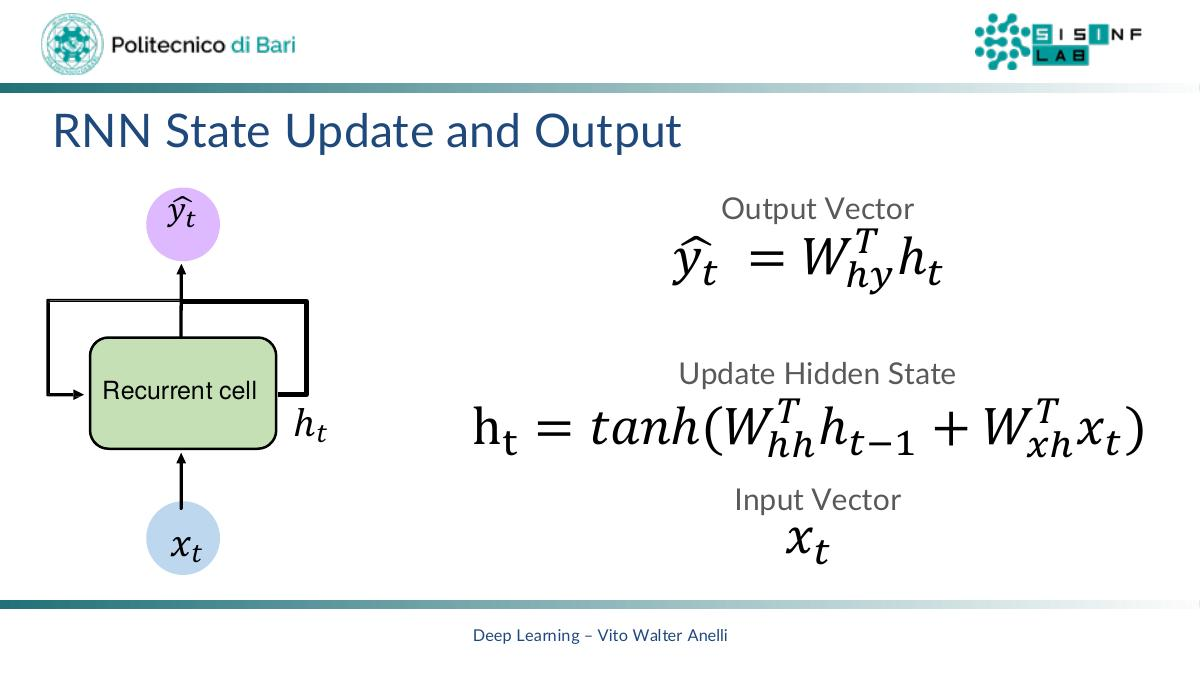
\includegraphics[width=0.82\linewidth]{figures/cf08_rnn_state_update.jpg}
  \caption{Cella ricorrente: sinistra, la rappresentazione compatta con il loop
           di ricorrenza; destra, le equazioni di aggiornamento dello stato
           nascosto $\mathbf{h}_t$ e di calcolo dell'output $\hat{\mathbf{y}}_t$.}
  \label{fig:rnn_state_update}
\end{figure}

\paragraph{Implementazione in PyTorch.}
\begin{lstlisting}[language=Python, caption={RNN minima in PyTorch.}, label={lst:rnn-pytorch}]
import torch.nn as nn

rnn = nn.RNN(input_size=d_x, hidden_size=d_h,
             num_layers=1, batch_first=True)
# output: (batch, seq_len, d_h), h_n: (1, batch, d_h)
output, h_n = rnn(x, h_0)
\end{lstlisting}

\subsection{Grafo Computazionale nel Tempo}
\label{subsec:unrolled-graph}

Una RNN può essere visualizzata come una rete feed-forward molto profonda
ottenuta \emph{srotolando} (\emph{unrolling}) la ricorrenza nel tempo. Ad ogni
passo temporale si inserisce un livello che condivide i pesi con tutti gli
altri. La loss totale è la somma delle loss ai singoli istanti:

\begin{equation}
  \mathcal{L} = \sum_{t=0}^{T} \mathcal{L}_t\!\left(\hat{\mathbf{y}}_t,
  \mathbf{y}_t\right).
  \label{eq:rnn-total-loss}
\end{equation}

\begin{figure}[H]
  \centering
  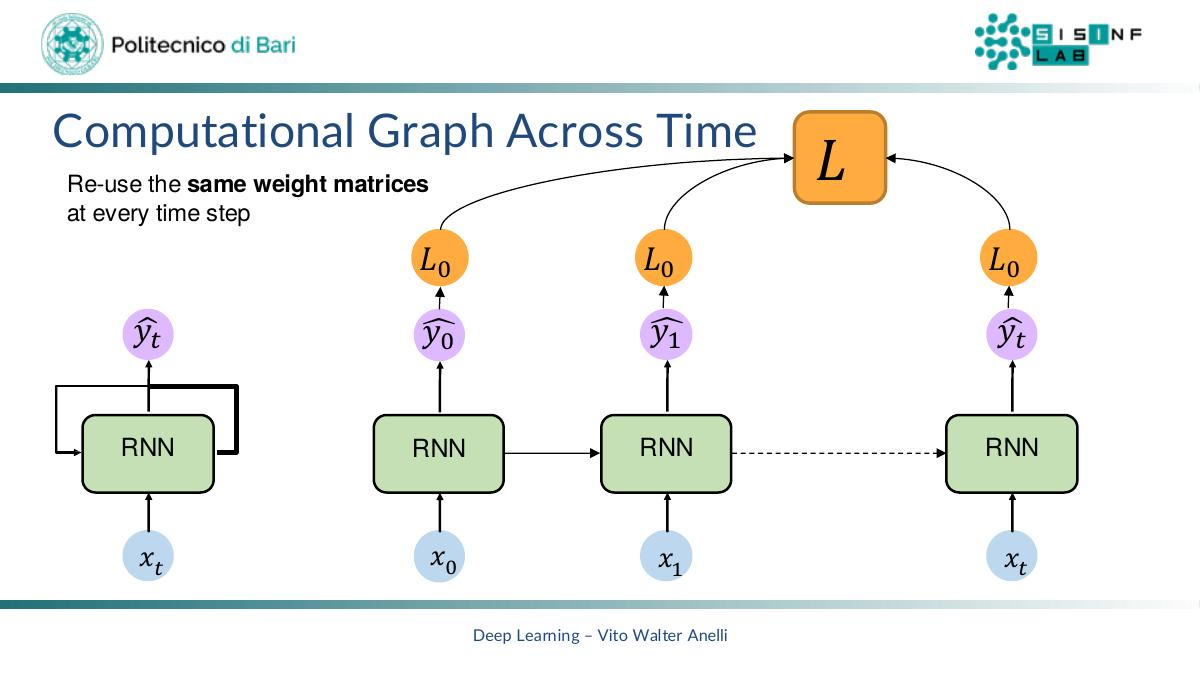
\includegraphics[width=0.82\linewidth]{figures/cf08_rnn_unrolled.jpg}
  \caption{Grafo computazionale di una RNN srotolato nel tempo. Le stesse
           matrici dei pesi $W_{hh}$, $W_{xh}$, $W_{hy}$ vengono riusate a ogni
           passo; la loss $\mathcal{L}$ è la somma delle loss parziali
           $\mathcal{L}_0, \mathcal{L}_1, \ldots$}
  \label{fig:rnn_unrolled}
\end{figure}

\subsection{Architetture Sequenziali}
\label{subsec:rnn-architectures}

A seconda del rapporto tra lunghezza dell'input e dell'output si distinguono:

\begin{description}
  \item[One-to-One] Rete vanilla senza ricorrenza.
  \item[Many-to-One] Una sequenza in ingresso produce un singolo output
        (es.\ classificazione del sentiment).
  \item[One-to-Many] Un singolo input produce una sequenza in uscita
        (es.\ generazione di musica o di testo).
  \item[Many-to-Many] Sequenza in ingresso, sequenza in uscita (es.\
        traduzione automatica, etichettatura POS).
\end{description}

%------------------------------------------------------------
\section{Backpropagation Through Time (BPTT)}
\label{sec:bptt}

\subsection{Algoritmo}
\label{subsec:bptt-algorithm}

Poiché la RNN srotolata è equivalente a una rete feed-forward con pesi
condivisi, la si può addestrare con la normale backpropagation applicata al
grafo computazionale nel tempo: è il cosiddetto algoritmo di
\textbf{Backpropagation Through Time (BPTT)} \citep{bishop2024}.

\begin{itemize}
  \item Il \emph{forward pass} scorre la sequenza da $t=0$ a $t=T$,
        costruendo uno stack delle attività nascoste $\mathbf{h}_0, \ldots,
        \mathbf{h}_T$.
  \item Il \emph{backward pass} disimpila le attività e calcola i gradienti
        dell'errore a ogni passo temporale.
  \item I gradienti rispetto a $W_{hh}$, $W_{xh}$, $W_{hy}$ vengono sommati
        su tutti i passi prima dell'aggiornamento.
\end{itemize}

Formalmente, il gradiente dell'errore rispetto allo stato nascosto al passo $t$
dipende da tutti i passi successivi:

\begin{equation}
  \frac{\partial \mathcal{L}}{\partial \mathbf{h}_t} =
  \frac{\partial \mathcal{L}_t}{\partial \mathbf{h}_t} +
  \frac{\partial \mathcal{L}}{\partial \mathbf{h}_{t+1}}
  \frac{\partial \mathbf{h}_{t+1}}{\partial \mathbf{h}_t}.
\end{equation}

\subsection{Il Problema dei Gradienti che Svaniscono o Esplodono}
\label{subsec:vanishing-exploding}

Il calcolo del gradiente rispetto allo stato nascosto iniziale $\mathbf{h}_0$
richiede il prodotto di $T$ fattori $W_{hh}$ (moltiplicazione matriciale
ripetuta). Questo genera due patologie simmetriche:

\begin{description}
  \item[Gradienti che svaniscono] Se i valori singolari di $W_{hh}$ sono
        $< 1$, il prodotto converge a zero esponenzialmente: le informazioni
        distanti nel tempo non riescono più a influenzare i pesi.
  \item[Gradienti che esplodono] Se i valori singolari sono $> 1$, il prodotto
        diverge: l'addestramento diventa instabile.
\end{description}

\begin{figure}[H]
  \centering
  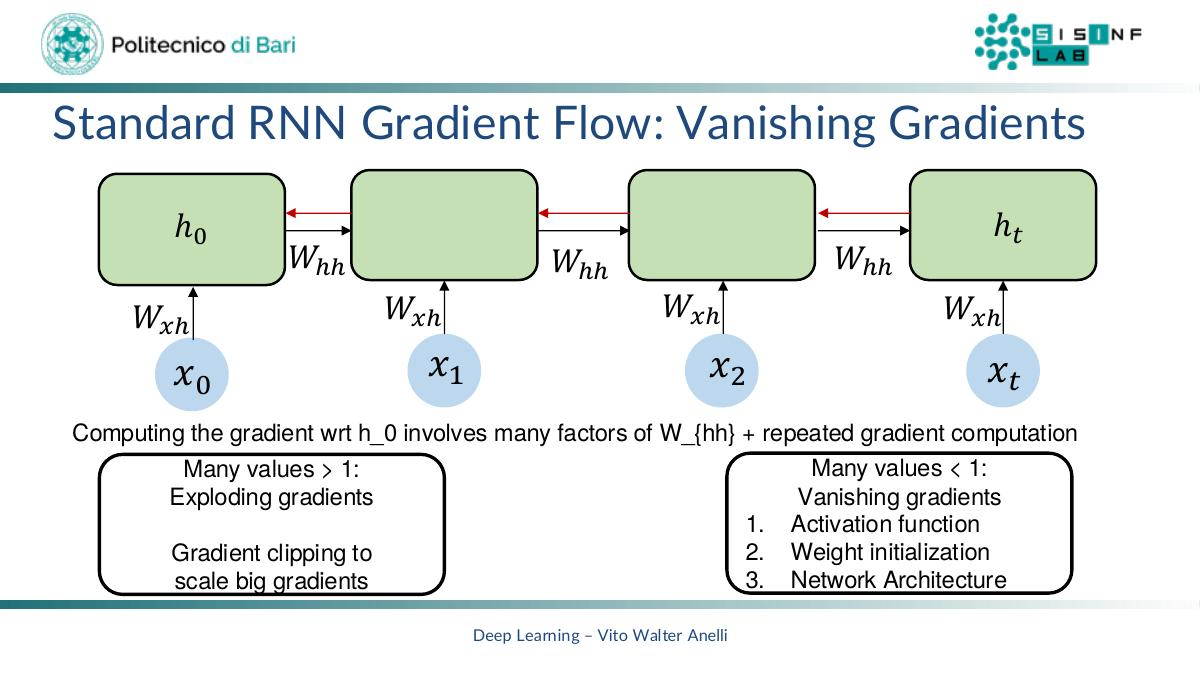
\includegraphics[width=0.82\linewidth]{figures/cf08_vanishing_gradients.jpg}
  \caption{Flusso del gradiente in una RNN standard. Le frecce rosse mostrano
           come il gradiente debba attraversare molte moltiplicazioni per
           $W_{hh}$ per raggiungere $\mathbf{h}_0$. Se $\|W_{hh}\| < 1$:
           vanishing; se $\|W_{hh}\| > 1$: exploding.}
  \label{fig:vanishing_gradients}
\end{figure}

\paragraph{Soluzioni pratiche.}
\begin{itemize}
  \item \textbf{Gradient clipping}: si riscalano i gradienti quando la loro
        norma supera una soglia $\theta$:
        $\nabla \leftarrow \frac{\theta}{\|\nabla\|}\,\nabla$ se
        $\|\nabla\| > \theta$. Mitiga l'esplosione.
  \item \textbf{Inizializzazione della matrice $W_{hh}$} come matrice ortogonale
        (valori singolari = 1): rallenta il collasso.
  \item \textbf{Architetture con gate} (LSTM, GRU): soluzione strutturale
        al problema del vanishing (Sezione \ref{sec:lstm}).
\end{itemize}

\paragraph{Nota sul backward pass lineare.}
A differenza del forward pass — dove funzioni di attivazione come $\tanh$
saturano e \emph{comprimono} i valori — il backward pass è localmente
\emph{lineare}: raddoppiare i gradienti all'uscita raddoppia tutti i gradienti
a ritroso nella rete. Questo amplifica la fragilità numerica del BPTT su
sequenze lunghe.

%------------------------------------------------------------
\section{Long Short-Term Memory (LSTM)}
\label{sec:lstm}

\subsection{Motivazione: La Memoria Analogica}
\label{subsec:lstm-motivation}

\citet{hochreiter1997lstm} propongono di risolvere il problema del vanishing
gradient introducendo una \textbf{cella di memoria} con connessioni lineari
di auto-rinforzo (peso di auto-collegamento uguale a 1) e \textbf{porte}
(\emph{gates}) che controllano selettivamente la scrittura, la lettura e la
cancellazione delle informazioni.

\begin{figure}[H]
  \centering
  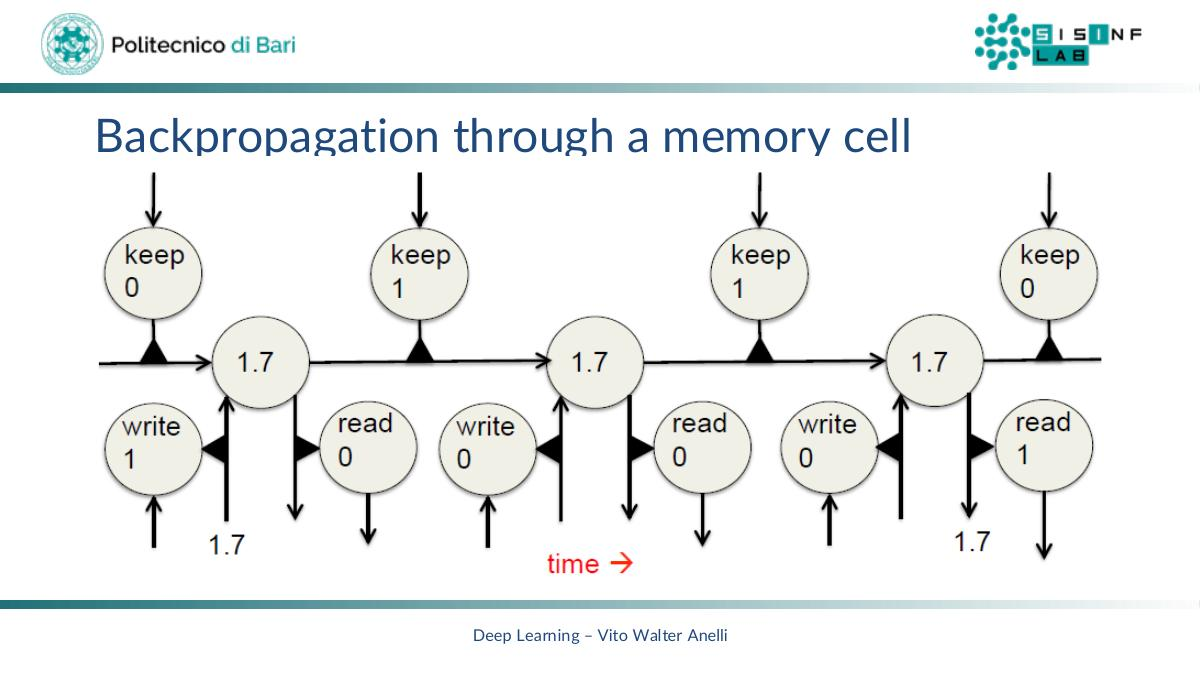
\includegraphics[width=0.82\linewidth]{figures/cf08_memory_cell_bptt.jpg}
  \caption{Cella di memoria analogica: il valore 1.7 viene scritto quando il
           gate \emph{write}~=~1, mantenuto finché \emph{keep}~=~1, e letto
           quando \emph{read}~=~1. La backpropagation attraversa questo
           circuito perché le porte logistiche hanno derivate ben definite.}
  \label{fig:memory_cell}
\end{figure}

\subsection{Architettura della Cella LSTM}
\label{subsec:lstm-architecture}

Una cella LSTM mantiene due vettori di stato distinti:
\begin{itemize}
  \item $\mathbf{c}_t \in \mathbb{R}^{d_h}$: \textbf{cell state}, la memoria
        a lungo termine.
  \item $\mathbf{h}_t \in \mathbb{R}^{d_h}$: \textbf{hidden state}, la memoria
        a breve termine e l'output della cella.
\end{itemize}

\begin{figure}[H]
  \centering
  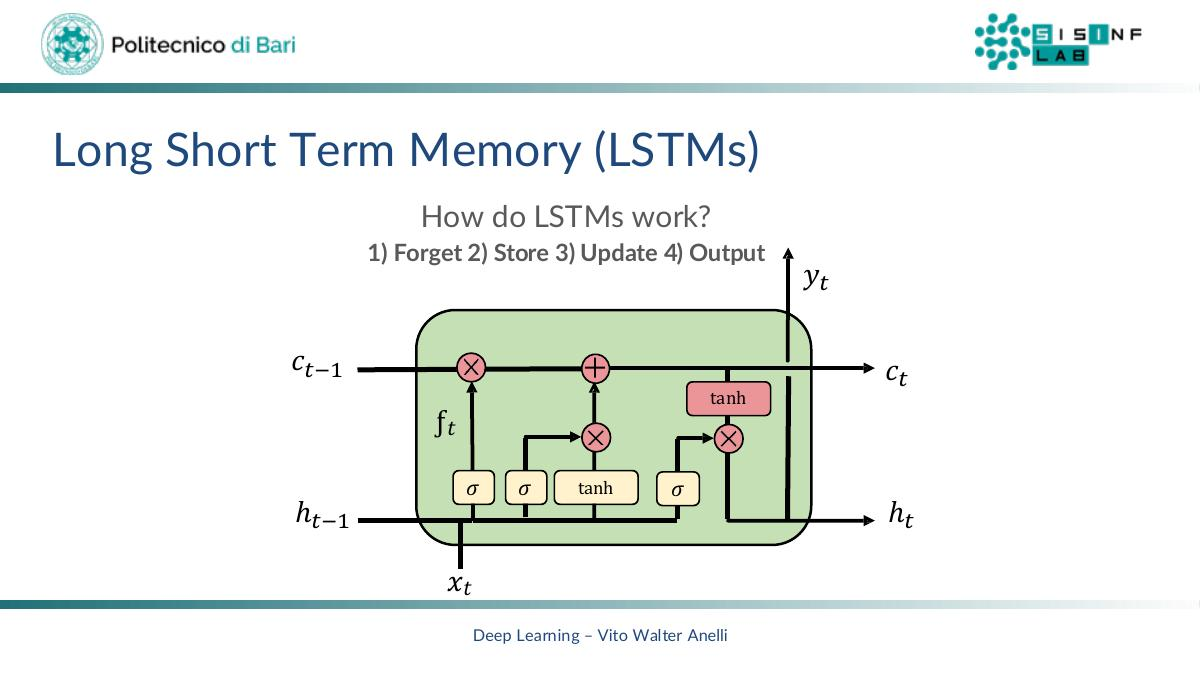
\includegraphics[width=0.75\linewidth]{figures/cf08_lstm_full.jpg}
  \caption{Schema completo della cella LSTM. Il cell state $\mathbf{c}_t$
           scorre orizzontalmente subendo solo operazioni element-wise
           (moltiplicazione e addizione), garantendo un flusso del gradiente
           non interrotto durante la BPTT.}
  \label{fig:lstm_full}
\end{figure}

Il comportamento della cella si articola in quattro fasi.

\subsubsection{Forget Gate (Cancellazione)}
\label{subsubsec:forget-gate}

Il forget gate decide quali informazioni eliminare dallo stato della cella:

\begin{equation}
  \mathbf{f}_t = \sigma\!\left(W_f \begin{bmatrix}\mathbf{h}_{t-1}\\
  \mathbf{x}_t\end{bmatrix} + \mathbf{b}_f\right),
  \label{eq:forget-gate}
\end{equation}

dove $\sigma$ è la sigmoide. Un valore $f_t^{(i)} \approx 0$ cancella
l'$i$-esima componente del cell state; $f_t^{(i)} \approx 1$ la conserva.

\begin{figure}[H]
  \centering
  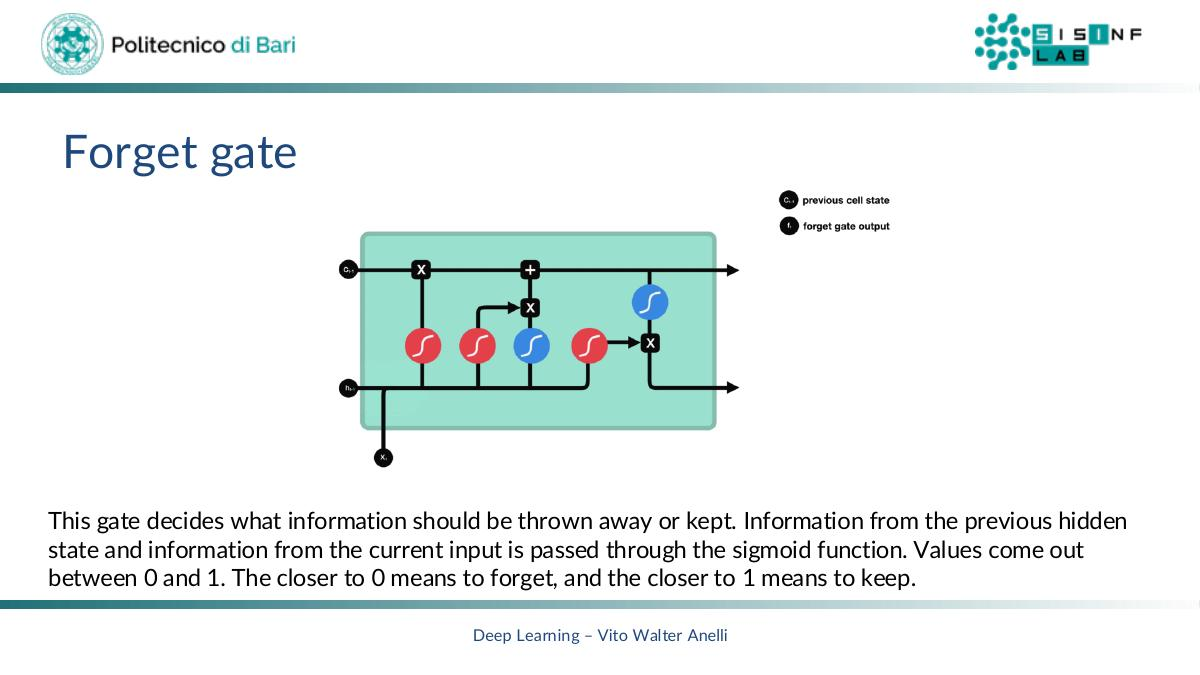
\includegraphics[width=0.70\linewidth]{figures/cf08_lstm_forget_gate.jpg}
  \caption{Forget gate: le attivazioni sigmoidee (in rosso) determinano quali
           informazioni del cell state precedente vengono eliminate (moltiplicazione
           per $\mathbf{f}_t$).}
  \label{fig:lstm_forget}
\end{figure}

\subsubsection{Input Gate (Memorizzazione)}
\label{subsubsec:input-gate}

Due sub-gate cooperano per aggiungere nuova informazione al cell state:

\begin{align}
  \mathbf{i}_t &= \sigma\!\left(W_i \begin{bmatrix}\mathbf{h}_{t-1}\\
                    \mathbf{x}_t\end{bmatrix} + \mathbf{b}_i\right),
  \label{eq:input-gate} \\
  \tilde{\mathbf{c}}_t &= \tanh\!\left(W_c \begin{bmatrix}\mathbf{h}_{t-1}\\
                    \mathbf{x}_t\end{bmatrix} + \mathbf{b}_c\right).
  \label{eq:candidate-cell}
\end{align}

$\mathbf{i}_t$ (gate sigmoid) seleziona quali componenti aggiornare;
$\tilde{\mathbf{c}}_t$ (gate tanh) genera il valore candidato da scrivere.

\subsubsection{Aggiornamento del Cell State}
\label{subsubsec:cell-update}

Il cell state viene aggiornato combinando la cancellazione e la scrittura
selettiva:

\begin{equation}
  \mathbf{c}_t = \mathbf{f}_t \odot \mathbf{c}_{t-1}
                + \mathbf{i}_t \odot \tilde{\mathbf{c}}_t,
  \label{eq:cell-update}
\end{equation}

dove $\odot$ indica il prodotto element-wise (Hadamard).

\subsubsection{Output Gate (Uscita)}
\label{subsubsec:output-gate}

L'output gate filtra il cell state per produrre il nuovo hidden state:

\begin{align}
  \mathbf{o}_t &= \sigma\!\left(W_o \begin{bmatrix}\mathbf{h}_{t-1}\\
                    \mathbf{x}_t\end{bmatrix} + \mathbf{b}_o\right),
  \label{eq:output-gate} \\
  \mathbf{h}_t &= \mathbf{o}_t \odot \tanh(\mathbf{c}_t).
  \label{eq:hidden-output}
\end{align}

\subsection{Flusso del Gradiente nelle LSTM}
\label{subsec:lstm-gradient}

Il punto cruciale delle LSTM è che la backpropagation da $\mathbf{c}_t$ a
$\mathbf{c}_{t-1}$ richiede \emph{solo operazioni element-wise} (moltiplicazione
per $\mathbf{f}_t$ e addizione); non c'è alcuna moltiplicazione matriciale lungo
il percorso del cell state. Di conseguenza:

\begin{itemize}
  \item Il gradiente scorre quasi indisturbato per centinaia di passi temporali
        (\emph{uninterrupted gradient flow}).
  \item Il forget gate impara a modulare il decay del gradiente in modo
        \emph{adattivo}: quando $\mathbf{f}_t \approx \mathbf{1}$ il gradiente
        viene interamente preservato; quando $\mathbf{f}_t \approx \mathbf{0}$
        la dipendenza dal passato viene eliminata.
\end{itemize}

\begin{lstlisting}[language=Python, caption={LSTM in PyTorch.}, label={lst:lstm-pytorch}]
import torch.nn as nn

lstm = nn.LSTM(input_size=d_x, hidden_size=d_h,
               num_layers=n_layers, batch_first=True)
# h_0, c_0: (n_layers, batch, d_h)
output, (h_n, c_n) = lstm(x, (h_0, c_0))
\end{lstlisting}

%------------------------------------------------------------
\section{Gated Recurrent Unit (GRU)}
\label{sec:gru}

\subsection{Architettura}
\label{subsec:gru-architecture}

La \textbf{Gated Recurrent Unit} \citep{cho2014gru} è una semplificazione delle
LSTM che elimina il cell state separato e usa solo due porte, riducendo il numero
di parametri e spesso raggiungendo prestazioni comparabili.

\paragraph{Reset gate.}
Il reset gate $\mathbf{r}_t$ controlla quanta memoria del passato viene
dimenticata nel calcolo del candidato:

\begin{equation}
  \mathbf{r}_t = \sigma\!\left(W_r\,[\mathbf{h}_{t-1};\,\mathbf{x}_t]
                 + \mathbf{b}_r\right).
  \label{eq:gru-reset}
\end{equation}

\paragraph{Update gate.}
Il update gate $\mathbf{z}_t$ determina in che misura il candidato
$\tilde{\mathbf{h}}_t$ sostituisce il vecchio hidden state:

\begin{equation}
  \mathbf{z}_t = \sigma\!\left(W_z\,[\mathbf{h}_{t-1};\,\mathbf{x}_t]
                 + \mathbf{b}_z\right).
  \label{eq:gru-update}
\end{equation}

\begin{figure}[H]
  \centering
  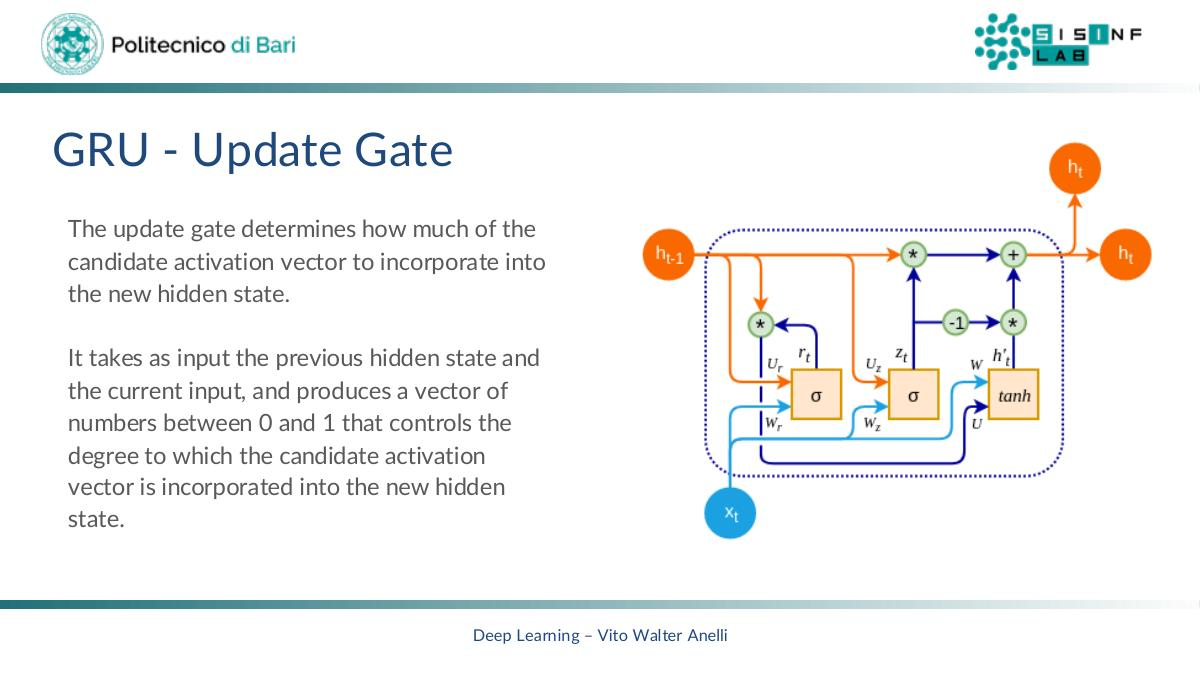
\includegraphics[width=0.72\linewidth]{figures/cf08_gru_update_gate.jpg}
  \caption{GRU: update gate $\mathbf{z}_t$ (a destra nel diagramma). Il
           vettore di output è una media pesata tra il vecchio stato e il
           candidato, con il bilanciamento controllato da $\mathbf{z}_t$.}
  \label{fig:gru_update}
\end{figure}

\paragraph{Candidato e aggiornamento.}

\begin{align}
  \tilde{\mathbf{h}}_t &= \tanh\!\left(W\,[\mathbf{r}_t \odot
                           \mathbf{h}_{t-1};\, \mathbf{x}_t]
                           + \mathbf{b}\right),
  \label{eq:gru-candidate} \\
  \mathbf{h}_t &= (\mathbf{1} - \mathbf{z}_t) \odot \mathbf{h}_{t-1}
                + \mathbf{z}_t \odot \tilde{\mathbf{h}}_t.
  \label{eq:gru-final}
\end{align}

L'equazione \eqref{eq:gru-final} mostra che la GRU interpola linearmente tra
lo stato vecchio e quello candidato: quando $\mathbf{z}_t \approx \mathbf{1}$
l'intero hidden state viene rimpiazzato; quando $\mathbf{z}_t \approx \mathbf{0}$
lo stato viene mantenuto intatto (effetto simile a quello dell'LSTM con forget
gate chiuso e input gate aperto).

\subsection{Confronto LSTM vs GRU}
\label{subsec:lstm-vs-gru}

\begin{table}[H]
  \centering
  \caption{Confronto tra LSTM e GRU.}
  \label{tab:lstm-gru}
  \small
  \begin{tabular}{lll}
    \toprule
    \textbf{Caratteristica} & \textbf{LSTM} & \textbf{GRU} \\
    \midrule
    Numero di porte & 3 (forget, input, output) & 2 (reset, update) \\
    Vettori di stato & 2 ($\mathbf{h}_t$, $\mathbf{c}_t$) & 1 ($\mathbf{h}_t$) \\
    Parametri per cella & $4 \times (d_h^2 + d_h d_x + d_h)$ & $3 \times (d_h^2 + d_h d_x + d_h)$ \\
    Vanishing gradient & Risolto (cell state lineare) & Risolto (interpolazione) \\
    Prestazioni tipiche & Migliori su sequenze lunghissime & Comparabili, più veloci \\
    \bottomrule
  \end{tabular}
\end{table}

%------------------------------------------------------------
\section{Bi-LSTM e Architetture Avanzate}
\label{sec:bilstm}

\subsection{LSTM Bidirezionale}
\label{subsec:bilstm}

Una \textbf{Bi-LSTM} elabora la sequenza in entrambe le direzioni temporali
(sinistra→destra e destra→sinistra) e concatena i due hidden state. Questo
consente all'output al passo $t$ di dipendere sia dal contesto passato che da
quello futuro. Formalmente:

\begin{align}
  \overrightarrow{\mathbf{h}}_t &= \mathrm{LSTM}_{\text{fwd}}(\mathbf{x}_t,
                                    \overrightarrow{\mathbf{h}}_{t-1}), \\
  \overleftarrow{\mathbf{h}}_t  &= \mathrm{LSTM}_{\text{bwd}}(\mathbf{x}_t,
                                    \overleftarrow{\mathbf{h}}_{t+1}), \\
  \mathbf{h}_t                  &= \left[\overrightarrow{\mathbf{h}}_t;\,
                                    \overleftarrow{\mathbf{h}}_t\right].
\end{align}

Le Bi-LSTM trovano ampio impiego in NLP per task come Named Entity Recognition
(NER), Part-of-Speech tagging e relazione semantica, dove il contesto futuro è
disponibile al momento dell'inferenza. Non sono adatte alla generazione
autoregressiva (la direzione futura non è disponibile durante il decoding).

\subsection{Encoder--Decoder per la Traduzione Automatica}
\label{subsec:seq2seq}

Il paradigma \textbf{sequence-to-sequence} (Seq2Seq) usa due RNN separate:

\begin{description}
  \item[Encoder] Legge la sequenza sorgente e la comprime in un vettore di
        contesto fisso $\mathbf{c} = \mathbf{h}_T^{\text{enc}}$.
  \item[Decoder] Genera la sequenza target autoregressivamente, condizionato
        su $\mathbf{c}$:
        $\mathbf{h}_t^{\text{dec}} = f(\mathbf{h}_{t-1}^{\text{dec}},
        \hat{y}_{t-1}, \mathbf{c})$.
\end{description}

Il vettore di contesto fisso costituisce un \textbf{collo di bottiglia}
informativo: per sequenze molto lunghe non riesce a codificare tutta
l'informazione rilevante. Questo limite motiva l'introduzione dei
\textbf{meccanismi di attenzione}, che permettono al decoder di accedere
direttamente a tutti gli hidden state dell'encoder pesandoli in modo
apprendibile \citep{bahdanau2015attention}.

%------------------------------------------------------------
\section{Applicazioni delle RNN}
\label{sec:rnn-applications}

\begin{description}
  \item[Generazione di musica] La rete riceve caratteri di notazione musicale
        e predice il prossimo carattere (schema many-to-many con teacher
        forcing durante l'addestramento).
  \item[Classificazione del sentiment] Una LSTM legge una sequenza di parole
        e l'ultimo hidden state viene passato a un classificatore lineare
        (many-to-one).
  \item[Traduzione automatica] Architettura Seq2Seq encoder--decoder, idealmente
        potenziata con attenzione.
  \item[Predizione di sequenze fisiche] Stima della traiettoria di oggetti in
        moto come predizione della prossima posizione di una pallina.
  \item[Modellazione del linguaggio] Calcolo della distribuzione di probabilità
        $P(w_t \mid w_1, \ldots, w_{t-1})$ alla base di modelli linguistici e
        sistemi di completamento automatico.
\end{description}

%------------------------------------------------------------
\section{Riepilogo e Linee Guida Pratiche}
\label{sec:rnn-summary}

\begin{table}[H]
  \centering
  \caption{Guida alla scelta dell'architettura ricorrente.}
  \label{tab:rnn_guide}
  \small
  \begin{tabular}{lll}
    \toprule
    \textbf{Scenario} & \textbf{Architettura} & \textbf{Note} \\
    \midrule
    Sequenze corte, baseline rapida & RNN vanilla & Instabile su $T > 20$ \\
    Dipendenze a lungo termine & LSTM & Standard de facto pre-Transformer \\
    Risorse computazionali limitate & GRU & Meno parametri, buona efficienza \\
    Contesto bidirezionale disponibile & Bi-LSTM & NER, POS tagging \\
    Traduzione, summarization & Seq2Seq + Attenzione & Precursore dei Transformer \\
    \bottomrule
  \end{tabular}
\end{table}

\paragraph{Consigli operativi.}
\begin{enumerate}
  \item Usare \textbf{gradient clipping} (norma soglia $\approx 5$) per tutte
        le RNN vanilla; nelle LSTM è meno critico ma consigliabile.
  \item Inizializzare $W_{hh}$ come matrice \textbf{ortogonale} per stabilizzare
        le prime fasi dell'addestramento.
  \item Preferire le \textbf{LSTM} alle RNN vanilla se la sequenza supera i 20--30
        passi; passare alle \textbf{GRU} per ridurre la memoria necessaria.
  \item Per l'NLP, usare un \textbf{learned embedding} pre-addestrato (es.\
        GloVe, FastText) come layer di input: riduce drasticamente i tempi di
        convergenza.
  \item Le RNN possono essere sostituite dai \textbf{Transformer} per molti task
        di sequenza, ma rimangono preferibili quando si ha memoria limitata, si
        lavora su dispositivi edge o quando la lunghezza della sequenza è molto
        variabile \citep{bishop2024}.
  \item Per il Seq2Seq, integrare sempre un \textbf{meccanismo di attenzione}:
        rompe il collo di bottiglia del vettore di contesto fisso e migliora
        significativamente la qualità delle traduzioni lunghe.
\end{enumerate}

%============================================================
%  Capitolo 9 – Migliorare la Generalizzazione
%============================================================
\chapter{Migliorare la Generalizzazione}
\label{ch:generalization}

Addestrare una rete neurale significa minimizzare la funzione di perdita sul
training set. Ma l'obiettivo reale è ottenere buone prestazioni su dati
\emph{mai visti} durante l'addestramento. La differenza tra errore di training
ed errore di test prende il nome di \textbf{gap di generalizzazione}: ridurlo è
il problema centrale del Deep Learning applicato \citep{bishop2024}.

%------------------------------------------------------------
\section{Il Problema dell'Overfitting}
\label{sec:overfitting-recap}

I dati di addestramento contengono due tipi di informazione:

\begin{enumerate}
  \item \textbf{Regolarità reali}: la struttura autentica della mappatura
        input→output che il modello deve apprendere.
  \item \textbf{Errore di campionamento}: fluttuazioni accidentali dovute al
        particolare sottoinsieme di esempi scelto per il training.
\end{enumerate}

Il modello non può distinguere tra le due: \emph{fitta entrambe}. Se la rete ha
capacità elevata, riesce a modellare anche il rumore campionario molto bene,
producendo curve di addestramento quasi perfette ma generalizzazione scarsa.
Questo fenomeno è l'\textbf{overfitting}.

\paragraph{Tre approcci principali per prevenirlo.}
\begin{description}
  \item[Più dati] Raccogliere ulteriori esempi è quasi sempre la strategia più
        efficace: con dati abbondanti l'errore di campionamento si riduce e il
        modello è costretto ad apprendere le regolarità vere.
  \item[Capacità giusta] Usare un'architettura abbastanza grande da catturare le
        regolarità reali, ma non tanto da fittare il rumore.
  \item[Media di modelli] Combinare le predizioni di molti modelli diversi riduce
        la varianza senza aumentare il bias.
\end{description}

%------------------------------------------------------------
\section{Metodi per Limitare la Capacità}
\label{sec:limit-capacity}

La \textbf{capacità effettiva} di una rete può essere controllata lungo
quattro assi, spesso combinati tra loro:

\begin{description}
  \item[Architettura] Limitare il numero di layer nascosti e di unità per layer.
        È la forma più diretta di controllo ma richiede una ricerca manuale
        dell'architettura ottimale.
  \item[Early stopping] Interrompere l'addestramento prima che il modello
        inizi a fittare il rumore di campionamento (Sezione
        \ref{sec:early-stopping}).
  \item[Weight decay] Penalizzare i pesi grandi con un termine aggiuntivo
        alla loss (Sezione \ref{sec:weight-decay}).
  \item[Rumore] Aggiungere rumore ai pesi o alle attivazioni durante il
        training (Sezione \ref{sec:noise-regularizer}).
\end{description}

%------------------------------------------------------------
\section{Early Stopping}
\label{sec:early-stopping}

\subsection{Intuizione: Capacità come Funzione dei Pesi}
\label{subsec:early-stopping-intuition}

Quando i pesi sono molto piccoli, ogni unità nascosta opera nella sua
\textbf{regione lineare}: l'attivazione sigmoide o tanh si comporta
approssimativamente come una funzione lineare per piccoli argomenti. Una
rete con sole trasformazioni lineari ha capacità espressiva limitata,
equivalente a un singolo layer lineare.

Man mano che i pesi crescono, le unità nascono a utilizzare la propria
\textbf{regione non lineare}, aumentando la capacità della rete. L'early
stopping sfrutta questa dinamica: partendo da pesi piccoli e interrompendo
l'addestramento abbastanza presto si ottiene una rete con capacità
efficace \emph{limitata}, anche se l'architettura dichiarata sarebbe molto
capiente.

\begin{figure}[H]
  \centering
  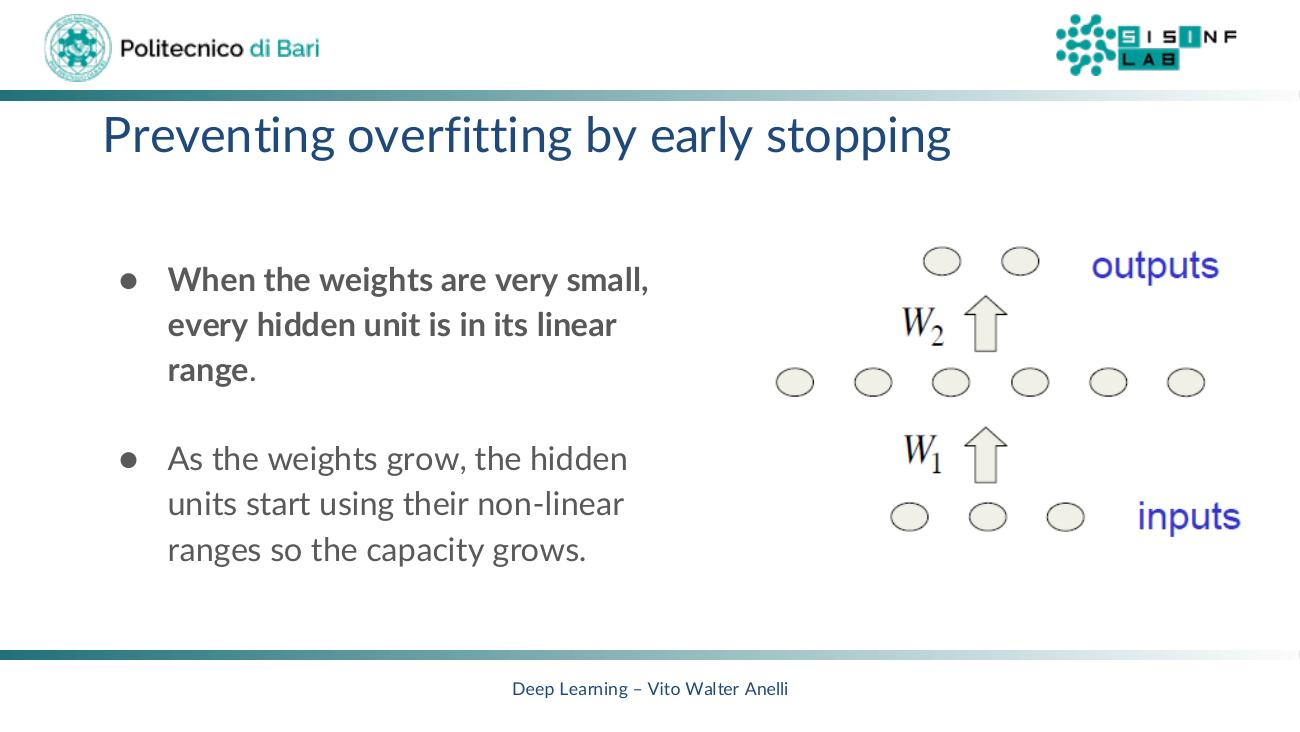
\includegraphics[width=0.72\linewidth]{figures/cf09_early_stopping_capacity.jpg}
  \caption{Early stopping e capacità. Con pesi piccoli ($W_1, W_2 \approx 0$)
           le unità nascoste sono nel regime lineare (bassa capacità). Al
           crescere dei pesi entrano nel regime non lineare e la capacità
           aumenta: fermarsi prima limita implicitamente la complessità del
           modello.}
  \label{fig:early_stopping}
\end{figure}

\subsection{Procedura Pratica}
\label{subsec:early-stopping-procedure}

\begin{enumerate}
  \item Tenere un \textbf{validation set} separato dal training set.
  \item Monitorare la validation loss a ogni epoch (o a intervalli regolari).
  \item Salvare i pesi ogni volta che la validation loss raggiunge un nuovo
        minimo (\emph{checkpoint}).
  \item Interrompere l'addestramento quando la validation loss non migliora
        per $k$ epoch consecutive (\emph{patience} $k$).
  \item Ripristinare i pesi del checkpoint migliore.
\end{enumerate}

\paragraph{Nota.} L'early stopping è concettualmente equivalente a una forma
di \emph{regolarizzazione implicita}: il numero di passi di aggiornamento svolge
lo stesso ruolo del coefficiente di penalizzazione in un problema di
ottimizzazione vincolata \citep{bishop2024}.

%------------------------------------------------------------
\section{Weight Decay (Regolarizzazione L2 e L1)}
\label{sec:weight-decay}

\subsection{Penalità L2}
\label{subsec:l2-penalty}

La \textbf{regolarizzazione L2} (o weight decay) aggiunge alla funzione di
costo un termine proporzionale alla somma dei quadrati dei pesi:

\begin{equation}
  \widetilde{\mathcal{L}}(\mathbf{w}) = \mathcal{L}(\mathbf{w})
    + \frac{\lambda}{2}\,\|\mathbf{w}\|^2
  = \mathcal{L}(\mathbf{w}) + \frac{\lambda}{2}\sum_i w_i^2.
  \label{eq:l2-loss}
\end{equation}

Il gradiente del termine di penalizzazione è $\lambda\,\mathbf{w}$, che si
sottrae ad ogni aggiornamento:

\begin{equation}
  w_i \leftarrow w_i - \eta\,\frac{\partial \mathcal{L}}{\partial w_i}
              - \eta\,\lambda\, w_i
  = w_i\,(1 - \eta\,\lambda) - \eta\,\frac{\partial\mathcal{L}}{\partial w_i}.
  \label{eq:l2-update}
\end{equation}

Il fattore $(1-\eta\lambda)$ riduce il peso ad ogni passo: i pesi rimangono
piccoli a meno che non contribuiscano a ridurre la loss, cioè a meno che
$\partial\mathcal{L}/\partial w_i$ sia grande. La penalità L2 corrisponde a
una \textbf{prior gaussiana} $p(w_i) \propto \exp(-\lambda w_i^2 / 2)$ nella
prospettiva bayesiana.

\subsection{Penalità L1}
\label{subsec:l1-penalty}

La \textbf{regolarizzazione L1} penalizza il valore assoluto dei pesi:

\begin{equation}
  \widetilde{\mathcal{L}}(\mathbf{w}) = \mathcal{L}(\mathbf{w})
    + \lambda\,\|\mathbf{w}\|_1
  = \mathcal{L}(\mathbf{w}) + \lambda\sum_i |w_i|.
  \label{eq:l1-loss}
\end{equation}

L'aggiornamento coinvolge il segno del peso:

\begin{equation}
  w_i \leftarrow w_i - \eta\,\frac{\partial\mathcal{L}}{\partial w_i}
              - \eta\,\lambda\,\operatorname{sign}(w_i).
  \label{eq:l1-update}
\end{equation}

La L1 tende a produrre soluzioni \textbf{sparse}: molti pesi vengono azzerati
esattamente. Equivale a una prior di Laplace $p(w_i) \propto
\exp(-\lambda|w_i|)$ e trova applicazione quando si desidera selezionare
automaticamente le feature rilevanti.

\begin{table}[H]
  \centering
  \caption{Confronto tra penalità L1 e L2.}
  \label{tab:l1-vs-l2}
  \small
  \begin{tabular}{lll}
    \toprule
    \textbf{Proprietà} & \textbf{L2 (Ridge)} & \textbf{L1 (Lasso)} \\
    \midrule
    Formula & $\lambda\sum w_i^2$ & $\lambda\sum |w_i|$ \\
    Effetto & Pesi piccoli ma non zero & Pesi sparsi (molti $= 0$) \\
    Prior bayesiana & Gaussiana & Laplace \\
    Derivabilità & Sì & No in $w_i=0$ \\
    Feature selection implicita & No & Sì \\
    Implementazione PyTorch & \texttt{weight\_decay} in optimizer & Penalità manuale \\
    \bottomrule
  \end{tabular}
\end{table}

%------------------------------------------------------------
\section{Rumore come Regolarizzatore}
\label{sec:noise-regularizer}

\subsection{Rumore Gaussiano sugli Input e L2 Implicita}
\label{subsec:gaussian-noise}

Aggiungere rumore gaussiano $\mathcal{N}(0, \sigma_i^2)$ all'input $x_i$ di
una rete semplice con unità di output lineare produce un effetto
regolarizzante equivalente alla penalità L2. La varianza del rumore viene
\emph{amplificata} dal quadrato del peso $w_i$ prima di contribuire all'uscita:

\begin{align}
  \tilde{x}_i &= x_i + \epsilon_i, \quad \epsilon_i \sim \mathcal{N}(0,\sigma_i^2),
  \label{eq:noisy-input} \\
  \tilde{y}_j &= y_j + \mathcal{N}(0, w_i^2 \sigma_i^2).
  \label{eq:noisy-output}
\end{align}

Minimizzare l'errore quadratico medio con input rumorosi equivale a minimizzare
l'errore quadratico medio originale più un termine $\sum_i w_i^2 \sigma_i^2$,
che è proporzionale alla penalità L2.

\begin{figure}[H]
  \centering
  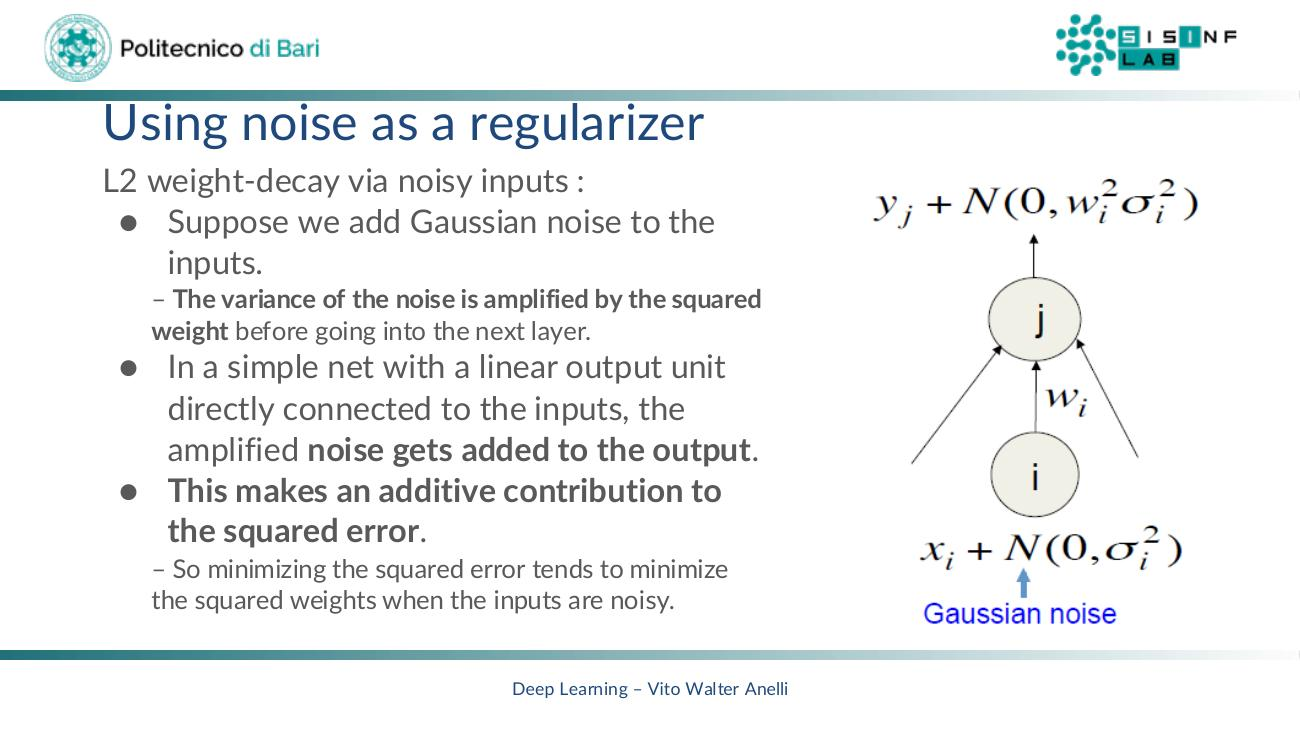
\includegraphics[width=0.62\linewidth]{figures/cf09_noise_regularizer.jpg}
  \caption{Rumore gaussiano come regolarizzatore L2. Il rumore sull'input
           $x_i \sim \mathcal{N}(0,\sigma_i^2)$ viene amplificato a
           $\mathcal{N}(0, w_i^2\sigma_i^2)$ nell'uscita $y_j$: minimizzare
           l'errore quadratico porta implicitamente a minimizzare $\sum_i w_i^2$.}
  \label{fig:noise_regularizer}
\end{figure}

\subsection{Forme di Rumore più Avanzate}
\label{subsec:advanced-noise}

Il rumore può essere applicato anche:
\begin{itemize}
  \item \textbf{Ai pesi} durante il forward pass: equivale ad una regolarizzazione
        sull'entropia della distribuzione dei pesi.
  \item \textbf{Alle attivazioni} dei layer nascosti: questa è la base del
        \textbf{Dropout} (Sezione \ref{sec:dropout}), dove il rumore ha la forma
        di una maschera binaria moltiplicativa.
\end{itemize}

%------------------------------------------------------------
\section{Combinare Modelli: Media degli Ensemble}
\label{sec:model-averaging}

\subsection{Bias-Variance Trade-off}
\label{subsec:bias-variance}

Per un problema di regressione, l'errore quadratico atteso si decompone in:

\begin{equation}
  \mathbb{E}\!\left[(y - \hat{y})^2\right]
  = \underbrace{\left(\mathbb{E}[\hat{y}] - y\right)^2}_{\text{Bias}^2}
  + \underbrace{\mathbb{E}\!\left[(\hat{y} - \mathbb{E}[\hat{y}])^2\right]}_{\text{Varianza}}
  + \sigma_\epsilon^2,
  \label{eq:bias-variance}
\end{equation}

dove $\sigma_\epsilon^2$ è la varianza del rumore irriducibile. La tabella
seguente riassume il trade-off:

\begin{table}[H]
  \centering
  \caption{Trade-off bias--varianza al variare della capacità del modello.}
  \label{tab:bias-variance}
  \small
  \begin{tabular}{lll}
    \toprule
    \textbf{Capacità} & \textbf{Bias} & \textbf{Varianza} \\
    \midrule
    Troppo bassa (underfitting) & Alto & Bassa \\
    Giusta & Basso & Bassa \\
    Troppo alta (overfitting) & Basso & Alta \\
    \bottomrule
  \end{tabular}
\end{table}

L'averaging di ensemble sfrutta il fatto che la \textbf{varianza di una media}
è inferiore alla varianza dei singoli modelli: combinando $M$ modelli
indipendenti con varianza $\sigma^2$ ciascuno si ottiene varianza $\sigma^2/M$.
Il bias invece non cambia. Si possono quindi usare modelli ad alta capacità
(basso bias, alta varianza) e ridurre la varianza via averaging
\citep{bishop2024}.

\subsection{Due Modi di Combinare i Modelli}
\label{subsec:mixture-product}

Dati $M$ modelli con distribuzione di output $P_m(y \mid \mathbf{x})$, esistono
due strategie di combinazione:

\paragraph{Mixture (media aritmetica).}
\begin{equation}
  P_{\text{mix}}(y \mid \mathbf{x}) = \frac{1}{M}\sum_{m=1}^{M} P_m(y \mid \mathbf{x}).
  \label{eq:mixture}
\end{equation}
La probabilità combinata è la media delle probabilità individuali. Corrisponde
a scegliere uniformemente uno dei modelli e campionare da esso.

\paragraph{Product (media geometrica).}
\begin{equation}
  P_{\text{prod}}(y \mid \mathbf{x}) \propto \prod_{m=1}^{M} P_m(y \mid \mathbf{x})
  = \exp\!\left(\frac{1}{M}\sum_{m=1}^{M} \log P_m(y \mid \mathbf{x})\right).
  \label{eq:product}
\end{equation}
La probabilità combinata è proporzionale al prodotto (o equivalentemente alla
media geometrica). È più \emph{conservativa}: assegna peso basso alle classi
che \emph{anche solo un} modello ritiene improbabili.

\begin{figure}[H]
  \centering
  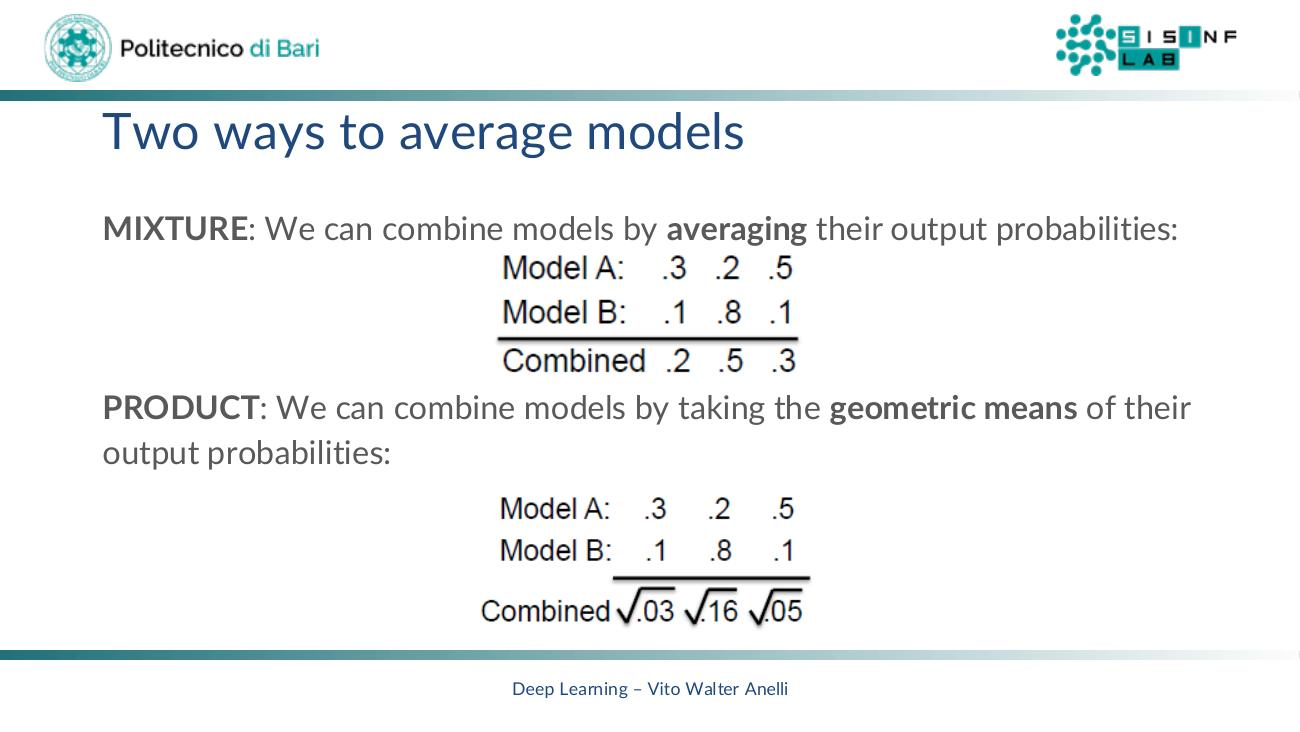
\includegraphics[width=0.70\linewidth]{figures/cf09_mixture_vs_product.jpg}
  \caption{Confronto numerico tra Mixture e Product su due modelli con tre
           classi. La mixture media aritmeticamente le probabilità; il product
           usa la media geometrica, producendo distribuzioni più concentrate
           sulle classi su cui i modelli concordano.}
  \label{fig:mixture_vs_product}
\end{figure}

\subsection{Come Rendere i Modelli Diversi}
\label{subsec:diverse-models}

Per massimizzare il beneficio dell'averaging, i modelli devono fare
\emph{errori diversi}. Le strategie principali sono:

\begin{description}
  \item[Bagging] Addestrare modelli diversi su sottoinsiemi estratti con
        rimpiazzo (\emph{bootstrap}). Le Random Forests applicano il bagging
        a alberi di decisione. Con reti neurali è molto costoso.
  \item[Boosting] Addestrare in sequenza modelli a bassa capacità, aumentando
        il peso degli esempi su cui i modelli precedenti hanno sbagliato. Focalizza
        le risorse computazionali sugli esempi difficili.
  \item[Diversità architetturale] Variare numero di layer, unità per layer,
        tipo di unità, tipo e forza della penalizzazione, algoritmo di
        ottimizzazione.
  \item[Diversità stocastica] Sfruttare la convergenza a minimi locali diversi
        in funzione dell'inizializzazione casuale (meno affidabile ma a costo zero).
\end{description}

%------------------------------------------------------------
\section{Dropout}
\label{sec:dropout}

\subsection{Definizione e Meccanismo}
\label{subsec:dropout-mechanism}

Il \textbf{Dropout} \citep{srivastava2014dropout} è una tecnica di
regolarizzazione che, a ogni forward pass durante il training, azzera
casualmente ciascuna unità nascosta con probabilità $p_{\text{drop}} = 1-p$
(dove $p$ è la \emph{keep probability}):

\begin{equation}
  \tilde{h}_i = m_i \cdot h_i, \quad
  m_i \sim \operatorname{Bernoulli}(p),
  \label{eq:dropout-mask}
\end{equation}

dove $\mathbf{m}$ è la \textbf{maschera} campionata indipendentemente per
ogni esempio e per ogni passo di training.

\begin{figure}[H]
  \centering
  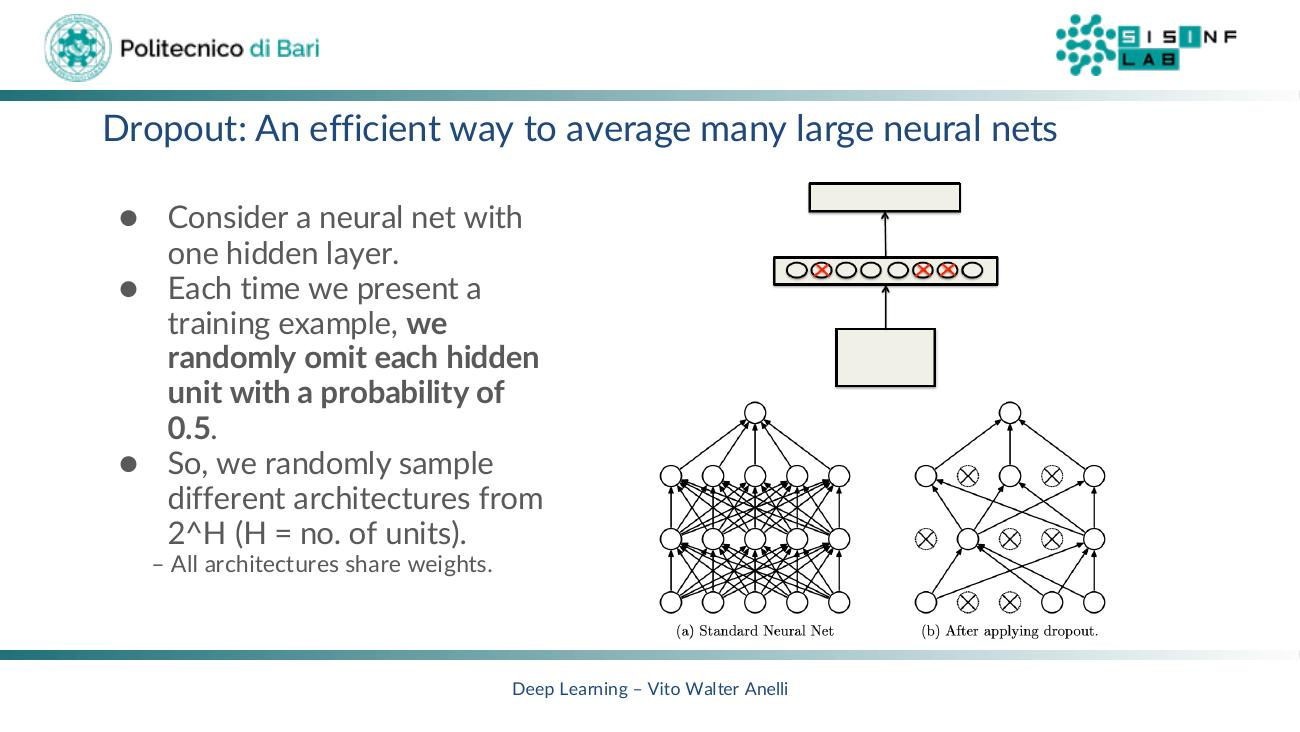
\includegraphics[width=0.82\linewidth]{figures/cf09_dropout_architecture.jpg}
  \caption{Dropout: (a) rete standard; (b) rete con dropout applicato -- le
           unità barrate (×) vengono annullate per quel forward pass. Con $H$
           unità nascoste si campiona tra $2^H$ sottoreti distinte, tutte con
           pesi condivisi.}
  \label{fig:dropout_arch}
\end{figure}

Con $H$ unità nascoste si esplorano fino a $2^H$ possibili sottoreti ad ogni
mini-batch. Tutte le sottoreti condividono gli stessi pesi, il che rappresenta
una regolarizzazione molto forte: ogni configurazione di pesi deve funzionare
bene per esponenzialmente molte architetture diverse.

\subsection{Dropout come Model Averaging}
\label{subsec:dropout-averaging}

Il Dropout può essere interpretato come una forma \emph{estrema} di bagging:
ogni sottorete viene addestrata su \emph{un solo} esempio (la configurazione di
maschera è unica per ogni forward pass). Rispetto al bagging classico i modelli
condividono però i pesi, il che li rende molto più fortemente regolarizzati di
quanto non farebbe la L2 o la L1 da soli.

\subsection{Inferenza a Tempo di Test: Weight Scaling}
\label{subsec:dropout-test}

Durante il test non si fa dropout: si usano \emph{tutte} le unità. Per
compensare il fatto che durante il training ogni unità era attiva solo con
probabilità $p$, i pesi in uscita vengono scalati:

\begin{equation}
  W_{\text{test}} = p \cdot W_{\text{train}}.
  \label{eq:weight-scaling}
\end{equation}

Questo garantisce che il valore atteso dell'attivazione a test time coincida
con quello a training time \citep{srivastava2014dropout}. In pratica, la
maggior parte dei framework (PyTorch, TensorFlow) implementa la variante
\textbf{inverted dropout}: durante il training i pesi \emph{attivi} vengono
divisi per $p$, così a test time non occorre alcun riscalamento:

\begin{equation}
  \tilde{h}_i = \frac{m_i \cdot h_i}{p}.
  \label{eq:inverted-dropout}
\end{equation}

\paragraph{Dropout multi-layer.}
Con più layer nascosti si applica dropout a ciascuno (tipicamente con $p = 0.5$
per i layer nascosti; $p = 0.8$--$0.9$ per il layer di input, che è più
sensibile alla perdita di features). Il modello medio (\emph{mean net}) con
tutti i pesi dimezzati non è esattamente la media geometrica di tutte le
sottoreti, ma è un'ottima approssimazione computazionalmente gratuita.

\paragraph{Dropout bayesiano (MC-Dropout).}
Eseguire il modello stocastico (con dropout attivo) $K$ volte sullo stesso
input durante il test fornisce una stima della \textbf{distribuzione di
incertezza} della predizione. Questa tecnica, nota come \emph{Monte Carlo
Dropout}, permette di quantificare l'incertezza predittiva senza richiedere
framework probabilistici complessi.

\subsection{Interpretazione della Co-Adattamento}
\label{subsec:coadaptation}

Un'unità nascosta che sa sempre quali altre unità sono presenti può
\emph{co-adattarsi}: specializzarsi in un compito che funziona solo in presenza
di un certo sottoinsieme di co-lavoratori. Tali co-adattazioni complesse sono
fragili su nuovi dati. Il Dropout rompe questo meccanismo: ogni unità deve
essere utile in combinazione con un insieme \emph{combinatorialmente diverso}
di co-lavoratori, il che la spinge a imparare feature autonomamente utili.

\begin{lstlisting}[language=Python, caption={Dropout in PyTorch.}, label={lst:dropout-pytorch}]
import torch.nn as nn

model = nn.Sequential(
    nn.Linear(d_in, d_h),
    nn.ReLU(),
    nn.Dropout(p=0.5),          # p = probabilita' di azzerare
    nn.Linear(d_h, d_h),
    nn.ReLU(),
    nn.Dropout(p=0.5),
    nn.Linear(d_h, d_out)
)

# Importante: attivare/disattivare il dropout correttamente
model.train()   # Dropout attivo
model.eval()    # Dropout disattivo (mean net)
\end{lstlisting}

%------------------------------------------------------------
\section{Riepilogo e Linee Guida Pratiche}
\label{sec:gen-summary}

\begin{table}[H]
  \centering
  \caption{Guida alla scelta della strategia di regolarizzazione.}
  \label{tab:regularization-guide}
  \small
  \begin{tabular}{lll}
    \toprule
    \textbf{Scenario} & \textbf{Strategia} & \textbf{Note} \\
    \midrule
    Dataset piccolo, modello semplice & L2 + Early Stopping & Baseline robusta \\
    Feature sparse / selezione & L1 (Lasso) & Produce pesi esattamente zero \\
    Reti profonde, dati medi & Dropout ($p=0.5$) & Standard per FC layers \\
    Reti convoluzionali & Batch Norm + Weight Decay & Dropout meno efficace nei conv \\
    Budget di compute limitato & Early Stopping & Costo zero aggiuntivo \\
    Incertezza predittiva & MC-Dropout & Stime probabilistiche \\
    Massima accuratezza disponibile & Ensemble + Dropout & Costoso ma efficace \\
    \bottomrule
  \end{tabular}
\end{table}

\paragraph{Regole operative.}
\begin{enumerate}
  \item Iniziare \textbf{sempre} con l'early stopping: non ha costo
        computazionale aggiuntivo e previene sprechi di addestramento.
  \item Aggiungere \textbf{weight decay} (L2) come regolarizzazione di base;
        usare AdamW che separa il weight decay dall'adattività del gradiente
        (cfr.\ Capitolo~\ref{ch:optimization}).
  \item Applicare \textbf{Dropout} nei layer fully-connected con $p = 0.5$;
        ridurre a $p = 0.2$--$0.3$ per layer convoluzionali o transformer,
        dove la ridondanza spaziale già regolarizza.
  \item Per la \textbf{stima dell'incertezza} usare MC-Dropout: fare $K = 30$
        --$100$ forward pass con dropout attivo e calcolare media e deviazione
        standard delle predizioni.
  \item Preferire \textbf{più dati} (o data augmentation) a regolarizzazioni
        aggressive: la regolarizzazione aiuta ma non sostituisce la ricchezza
        informativa del dataset.
  \item Ricordare di chiamare \texttt{model.eval()} prima dell'inferenza
        in PyTorch: altrimenti il Dropout rimane attivo e le predizioni
        risultano stocastiche e sub-ottimali.
\end{enumerate}

Come notato da \citet{bishop2024}, le tecniche di regolarizzazione non vanno
considerate alternative esclusive: la combinazione di early stopping, weight
decay e dropout è la norma nei moderni sistemi di deep learning ad alte
prestazioni.

%============================================================
%  Capitolo 10 – Autoencoder
%============================================================
\chapter{Autoencoder}
\label{ch:autoencoders}

Gli autoencoder sono reti neurali addestrate a riprodurre il proprio input
all'uscita. L'obiettivo apparente è banale ($h_\theta(\mathbf{x}) \approx
\mathbf{x}$), ma l'interesse non risiede nell'output bensì nella
\textbf{rappresentazione interna} appresa durante il processo. Imponendo
opportuni vincoli sul collo di bottiglia centrale, la rete è costretta a
estrarre una rappresentazione compatta e informativa dei dati,
utile per compressione, riduzione dimensionale, generazione e
pre-addestramento non supervisionato \citep{bishop2024}.

%------------------------------------------------------------
\section{Autoencoder Classico}
\label{sec:ae-classic}

\subsection{Struttura e Formulazione}
\label{subsec:ae-structure}

Un autoencoder è composto da due sotto-reti simmetriche:

\begin{description}
  \item[Encoder] $e_\phi : \mathbb{R}^d \to \mathbb{R}^k$ con $k \ll d$,
        mappa l'input $\mathbf{x}$ in una rappresentazione latente
        $\mathbf{z} = e_\phi(\mathbf{x})$.
  \item[Decoder] $d_\psi : \mathbb{R}^k \to \mathbb{R}^d$, ricostruisce
        l'input dalla rappresentazione latente: $\hat{\mathbf{x}} =
        d_\psi(\mathbf{z})$.
\end{description}

La loss di addestramento è l'\textbf{errore di ricostruzione}:

\begin{equation}
  \mathcal{L}_{\text{rec}} = \frac{1}{N}\sum_{n=1}^{N}
    \bigl\|d_\psi(e_\phi(\mathbf{x}_n)) - \mathbf{x}_n\bigr\|^2.
  \label{eq:ae-rec-loss}
\end{equation}

Senza vincoli aggiuntivi la rete potrebbe imparare la funzione identità
in modo banale (es.\ con pesi unitari). La soluzione interessante emerge
solo quando si impone che lo strato intermedio abbia dimensionalità ridotta
($k < d$, \emph{undercomplete autoencoder}) o che le attivazioni siano
sparse (\emph{sparse autoencoder}).

\begin{figure}[H]
  \centering
  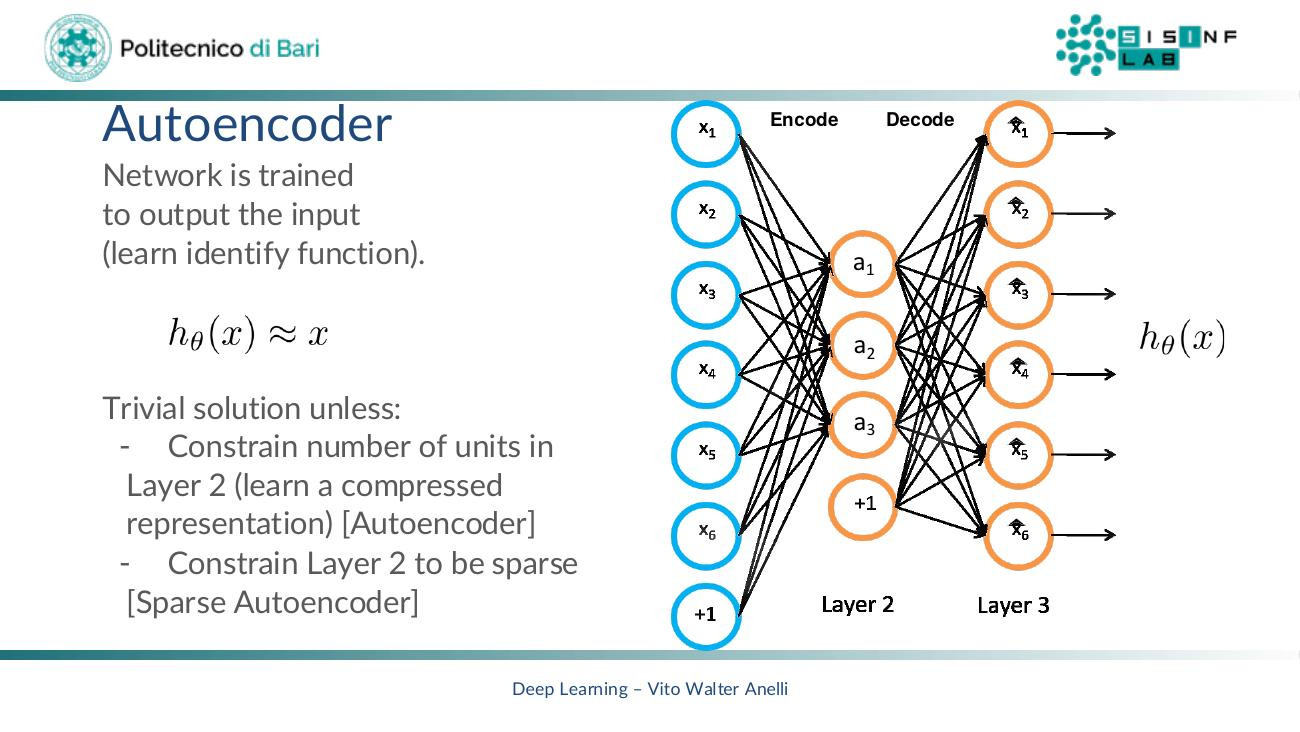
\includegraphics[width=0.82\linewidth]{figures/cf10_ae_architecture.jpg}
  \caption{Architettura di un autoencoder con 6 neuroni di input, 3 unità
           latenti $a_1, a_2, a_3$ (Layer~2) e 6 neuroni di output (Layer~3).
           La rete apprende la funzione $h_\theta(\mathbf{x}) \approx
           \mathbf{x}$ attraverso il collo di bottiglia.}
  \label{fig:ae_architecture}
\end{figure}

\subsection{Sparse Autoencoder}
\label{subsec:sparse-ae}

Nello \textbf{sparse autoencoder} la dimensionalità del collo di bottiglia
può anche essere maggiore di quella dell'input ($k > d$,
\emph{overcomplete}), ma le attivazioni latenti vengono penalizzate con un
termine L1 che le forza a essere sparse:

\begin{equation}
  \mathcal{L}_{\text{sparse}} = \underbrace{\|h_\theta(\mathbf{x}) -
    \mathbf{x}\|^2}_{\text{errore di ricostruzione}}
    + \lambda \underbrace{\sum_{i} |a_i|}_{\text{termine L1 di sparsità}},
  \label{eq:sparse-ae-loss}
\end{equation}

dove $a_i$ è l'attivazione dell'$i$-esima unità latente. Il vincolo
di sparsità induce la rete a usare solo poche unità attive per ogni
esempio, producendo una rappresentazione distribuita e interpretabile.
Questa formulazione è strettamente collegata alla \emph{dictionary
learning} e ai metodi di codifica sparsa \citep{bishop2024}.

%------------------------------------------------------------
\section{Deep Autoencoder}
\label{sec:deep-ae}

\subsection{Stacking di Autoencoder}
\label{subsec:stacking}

La profondità può essere aumentata impilando più coppie encoder-decoder.
Ogni livello impara una rappresentazione sempre più astratta dell'input;
i pesi dei livelli di decodifica sono tipicamente condivisi (o trasposti)
rispetto ai livelli di codifica (\emph{tied weights}):

\begin{equation}
  W_{\text{dec},\ell} = W_{\text{enc},\ell}^T.
  \label{eq:tied-weights}
\end{equation}

\begin{figure}[H]
  \centering
  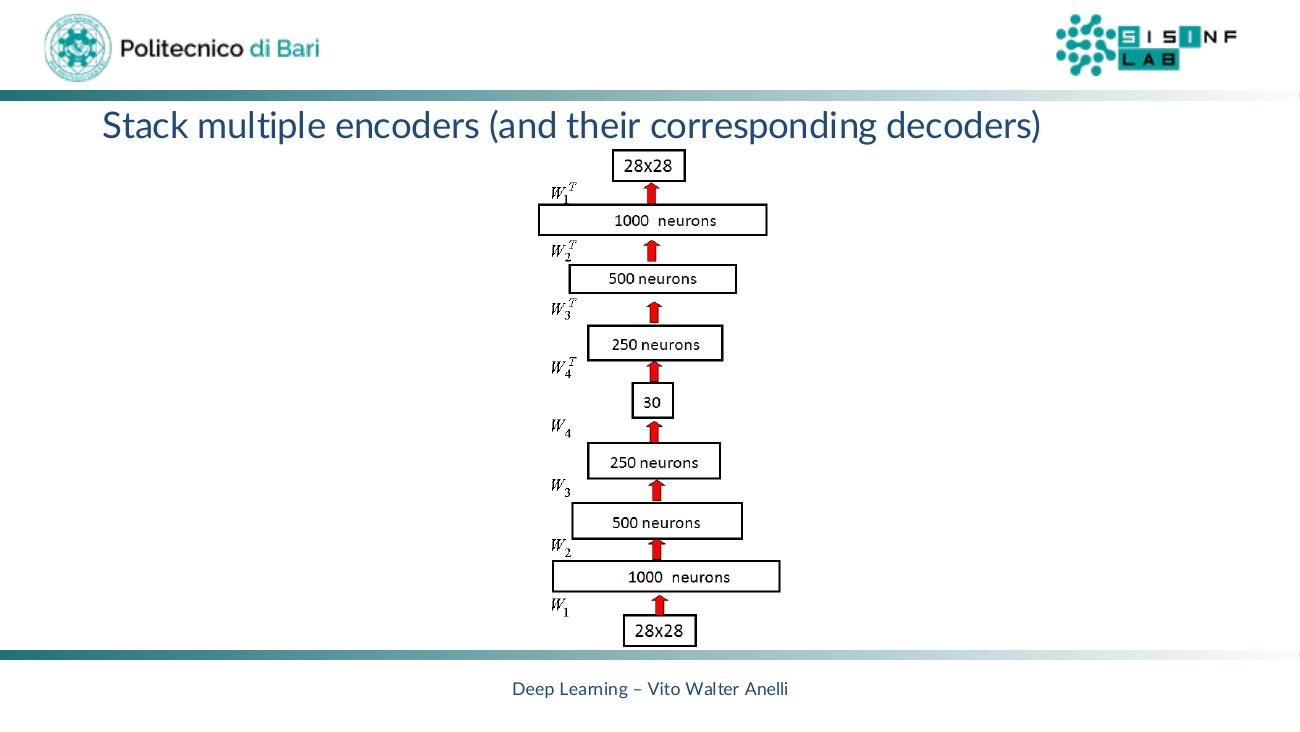
\includegraphics[width=0.55\linewidth]{figures/cf10_deep_ae_stacked.jpg}
  \caption{Deep autoencoder per immagini $28\times28$ (MNIST): il percorso
           di codifica comprime $784 \to 1000 \to 500 \to 250 \to 30$
           neuroni; il percorso di decodifica (con pesi $W_i^T$) ricostruisce
           simmetricamente fino alla dimensione originale.}
  \label{fig:deep_ae}
\end{figure}

\subsection{Confronto con la PCA}
\label{subsec:ae-vs-pca}

Un autoencoder lineare a un livello nascosto apprende esattamente lo
stesso sottospazio della \textbf{PCA}: il collo di bottiglia proietta
i dati sulle $k$ componenti principali a maggiore varianza. Un autoencoder
\emph{non lineare} (con funzioni di attivazione) apprende una varietà
non lineare, catturando strutture più complesse.

\begin{figure}[H]
  \centering
  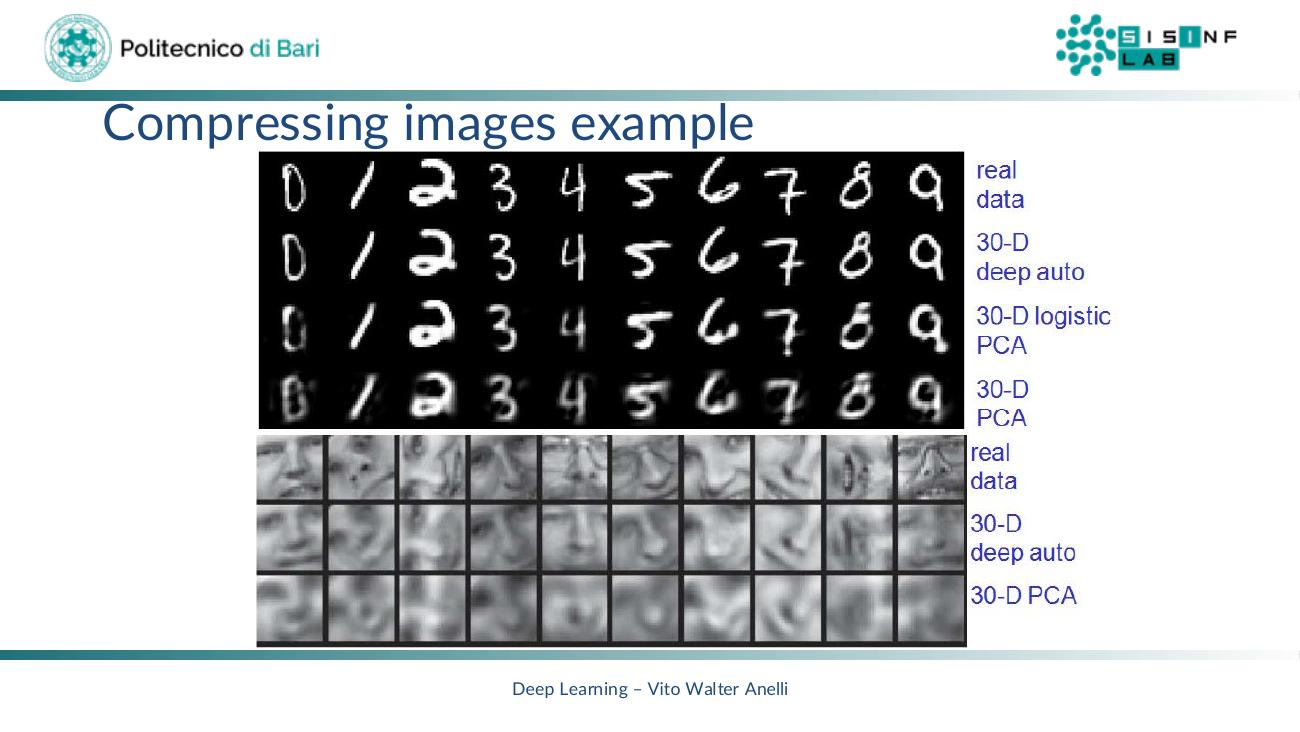
\includegraphics[width=0.82\linewidth]{figures/cf10_ae_compression_mnist.jpg}
  \caption{Compressione a 30 dimensioni su MNIST (sopra) e su volti
           (sotto). Il deep autoencoder (riga 2) preserva dettagli fini che
           la PCA lineare a 30 componenti (riga~4) non riesce a catturare,
           confermando la superiorità delle rappresentazioni non lineari.}
  \label{fig:ae_compression}
\end{figure}

%------------------------------------------------------------
\section{U-Net}
\label{sec:unet}

\subsection{Segmentazione Semantica}
\label{subsec:semantic-segmentation}

La \textbf{segmentazione semantica} è il compito di assegnare una classe
a ogni singolo pixel di un'immagine. I modelli sono addestrati usando
\emph{mappe di segmentazione} come target: per ogni immagine si dispone
di una mappa binaria che distingue i pixel di interesse (es.\ cellule
biologiche) da quelli di sfondo. La perdita tipica per questa formulazione
è la \textbf{cross-entropy binaria} pixel-per-pixel o la
\textbf{Dice loss}, che massimizza la sovrapposizione tra maschera
predetta e maschera vera.

\subsection{Architettura U-Net}
\label{subsec:unet-architecture}

La \textbf{U-Net} \citep{ronneberger2015unet} è un autoencoder
convoluzionale progettato per la segmentazione semantica, originariamente
concepita per immagini medicali. La struttura simmetrica a forma di U
comprende tre componenti:

\begin{description}
  \item[Percorso contrattivo (Encoder)] Sequenze di blocchi convoluzionali
        seguiti da max-pooling; riduce progressivamente la risoluzione
        spaziale aumentando il numero di feature map.
  \item[Percorso espansivo (Decoder)] Blocchi di deconvoluzione
        (convoluzione trasposta) che ripristinano la risoluzione spaziale,
        alternati a convoluzioni standard.
  \item[Skip connections] Connessioni dirette che concatenano le feature
        map del percorso contrattivo al livello corrispondente del percorso
        espansivo.
\end{description}

\begin{figure}[H]
  \centering
  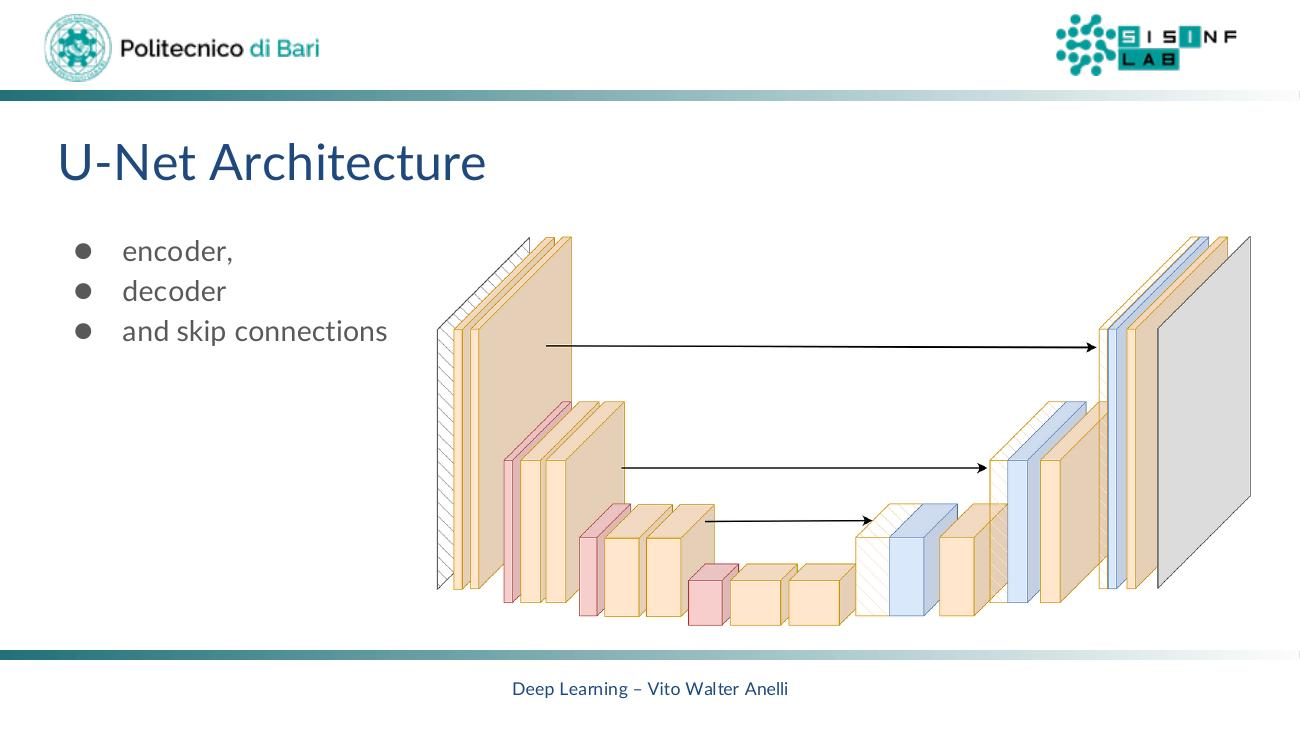
\includegraphics[width=0.82\linewidth]{figures/cf10_unet_architecture.jpg}
  \caption{Architettura U-Net: la forma a U è evidente dalla progressiva
           riduzione spaziale nel percorso di sinistra (encoder) e dalla
           riespansione nel percorso di destra (decoder). Le frecce
           orizzontali rappresentano le skip connections.}
  \label{fig:unet_arch}
\end{figure}

\subsection{Skip Connections}
\label{subsec:skip-connections}

Le skip connections sono la differenza architettonica cruciale rispetto
a un autoencoder classico, nel quale encoder e decoder devono essere
strettamente separati (altrimenti la compressione non avrebbe senso).
Nella U-Net questa restrizione non esiste: l'output è una mappa di
segmentazione della \emph{stessa risoluzione} dell'input, non una
ricostruzione.

Ogni skip connection concatena l'ultimo feature map del blocco
convoluzionale $k$ con l'output del blocco deconvoluzionale
corrispondente, fornendo due tipi di informazione complementari:

\begin{itemize}
  \item \textbf{Estrazione di feature}: le feature ad alto livello
        apprese nel percorso espansivo.
  \item \textbf{Localizzazione}: la posizione spaziale delle feature
        estratte dal corrispondente livello convoluzionale dell'encoder.
\end{itemize}

\begin{figure}[H]
  \centering
  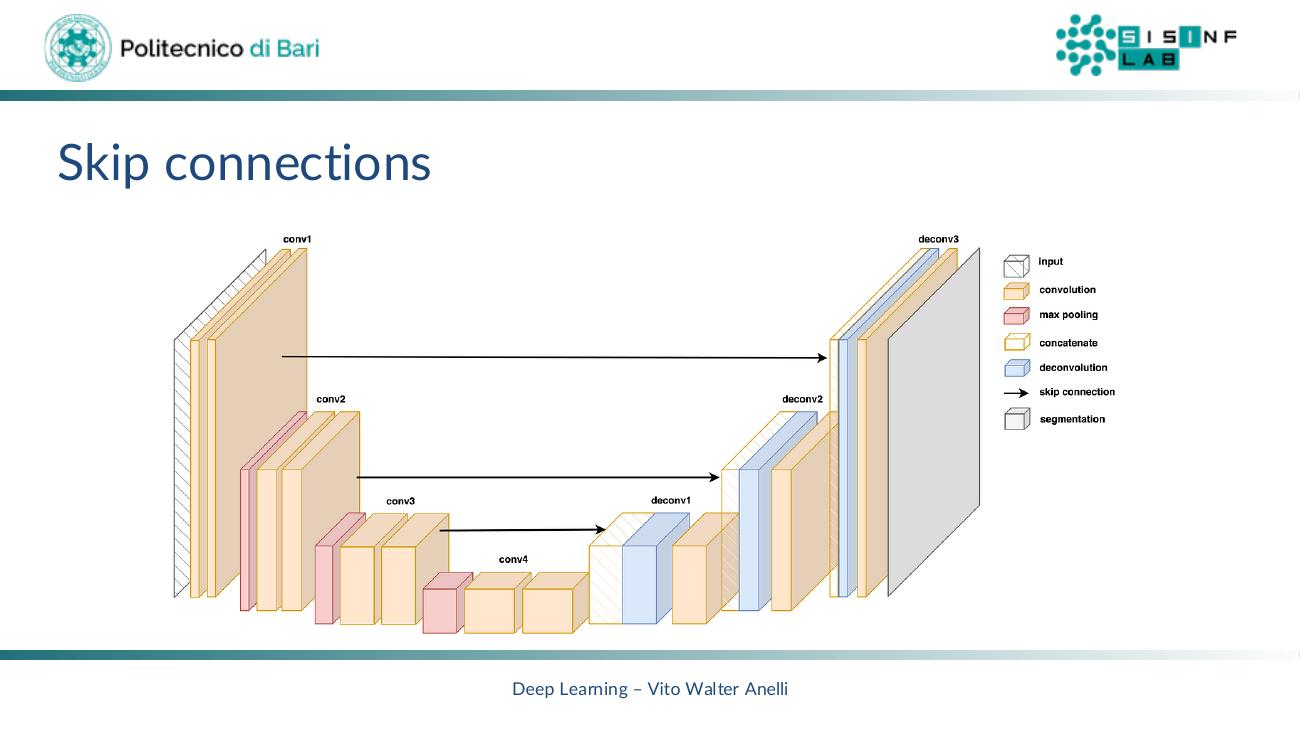
\includegraphics[width=0.82\linewidth]{figures/cf10_unet_skip_connections.jpg}
  \caption{Skip connections nella U-Net: ogni freccia orizzontale
           (conv\,1$\to$deconv\,3, conv\,2$\to$deconv\,2, conv\,3$\to$deconv\,1)
           concatena la mappa del livello convoluzionale con quella del
           corrispondente livello deconvoluzionale, combinando localizzazione
           e semantica.}
  \label{fig:unet_skip}
\end{figure}

\subsection{Deconvoluzione e Upsampling}
\label{subsec:deconvolution}

Il percorso espansivo utilizza \textbf{convoluzione trasposta}
(\emph{deconvolution} o \emph{transposed convolution}) per aumentare
la risoluzione spaziale in modo apprendibile, a differenza del
max-pooling che usa una regola fissa. In Keras/TensorFlow:

\begin{lstlisting}[language=Python, caption={Blocco espansivo U-Net in
  Keras.}, label={lst:unet-block}]
deconv = Conv2DTranspose(filters, (3,3),
                         strides=(2,2), padding="same")(prev)
uconv  = concatenate([deconv, skip_conv])   # skip connection
uconv  = Dropout(0.5)(uconv)
uconv  = Conv2D(filters, (3,3), activation="relu",
                padding="same")(uconv)
uconv  = Conv2D(filters, (3,3), activation="relu",
                padding="same")(uconv)
\end{lstlisting}

\paragraph{Layer di output.}
Il layer finale è una convoluzione $1\times1$ con attivazione sigmoide
che mappa ogni pixel a una probabilità di appartenenza alla classe
target. Nella U-Net \emph{non sono presenti layer fully-connected}:
l'intera rete è \emph{fully convolutional}, il che la rende applicabile
a immagini di dimensioni arbitrarie.

\begin{lstlisting}[language=Python, caption={Layer di output U-Net.},
  label={lst:unet-output}]
output = Conv2D(1, (1,1), padding="same",
                activation="sigmoid")(uconv1)
\end{lstlisting}

%------------------------------------------------------------
\section{Variational Autoencoder (VAE)}
\label{sec:vae}

\subsection{Limitazioni dell'Autoencoder Classico}
\label{subsec:ae-limitations}

Nell'autoencoder classico il collo di bottiglia mappa ogni input in un
\emph{punto} dello spazio latente. Campionare un punto arbitrario da
tale spazio e decodificarlo non produce necessariamente output
semanticamente significativi: lo spazio latente non è strutturato in
modo da garantire \emph{continuità} (punti vicini $\Rightarrow$ output
simili) né \emph{completezza} (ogni punto è decodificabile
in modo sensato). Il VAE risolve questi limiti imponendo una
\textbf{regolarizzazione probabilistica} sullo spazio latente.

\subsection{Confronto AE vs VAE: Flusso Computazionale}
\label{subsec:ae-vs-vae}

\begin{figure}[H]
  \centering
  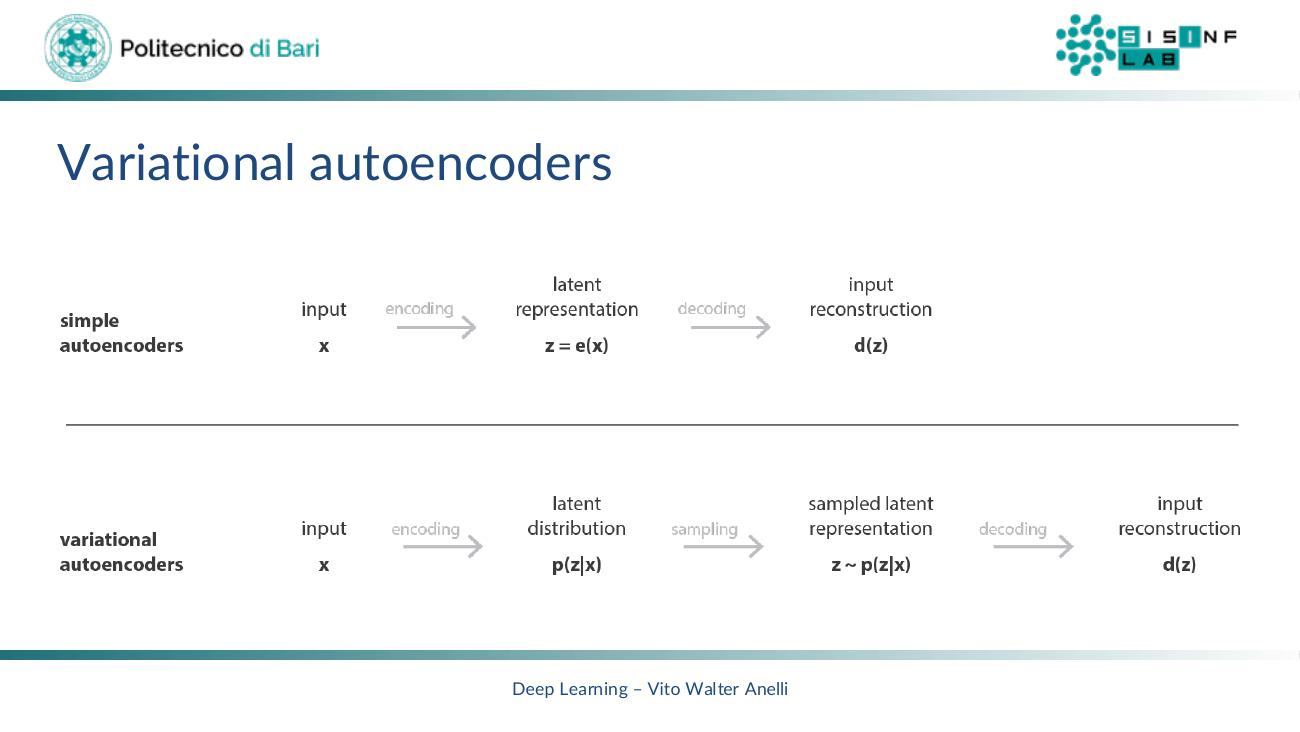
\includegraphics[width=0.82\linewidth]{figures/cf10_ae_vs_vae_flow.jpg}
  \caption{Confronto tra autoencoder classico (sopra) e variazionale
           (sotto). Nell'AE classico l'encoder produce un punto
           $\mathbf{z} = e(\mathbf{x})$; nel VAE produce una
           \emph{distribuzione} $p(\mathbf{z}|\mathbf{x})$, da cui viene
           campionato $\mathbf{z}$ prima della decodifica.}
  \label{fig:ae_vs_vae}
\end{figure}

\subsection{Modello Probabilistico}
\label{subsec:vae-probabilistic}

Il VAE \citep{kingma2014vae} adotta una prospettiva generativa. Si
definiscono due variabili:

\begin{itemize}
  \item $\mathbf{x}$: i dati osservati.
  \item $\mathbf{z}$: variabile latente \emph{non osservata} (rappresentazione
        compressa).
\end{itemize}

Il processo generativo assume:

\begin{align}
  p(\mathbf{z}) &\equiv \mathcal{N}(\mathbf{0}, \mathbf{I})
    \quad \text{(prior standard gaussiana)},
  \label{eq:vae-prior} \\
  p(\mathbf{x}|\mathbf{z}) &\equiv \mathcal{N}(f(\mathbf{z}),\, c\mathbf{I})
    \quad f \in F,\; c > 0
  \label{eq:vae-likelihood}
\end{align}

dove $f$ è la funzione \textbf{decoder} (una rete neurale) e $c$ è un
iperparametro di scala della varianza. Si ridefiniscono encoder e decoder
in termini probabilistici:

\begin{description}
  \item[Decoder probabilistico] $p(\mathbf{x}|\mathbf{z})$: distribuzione
        della variabile decodificata dato il codice.
  \item[Encoder probabilistico] $p(\mathbf{z}|\mathbf{x})$: distribuzione
        della variabile latente dato l'input (posteriore di Bayes).
\end{description}

\paragraph{Il teorema di Bayes nel VAE.}
Per il teorema di Bayes:

\begin{equation}
  p(\mathbf{z}|\mathbf{x}) = \frac{p(\mathbf{x}|\mathbf{z})\,p(\mathbf{z})}{p(\mathbf{x})}
  = \frac{p(\mathbf{x}|\mathbf{z})\,p(\mathbf{z})}{\displaystyle\int p(\mathbf{x}|\mathbf{u})\,p(\mathbf{u})\,d\mathbf{u}}.
  \label{eq:bayes-vae}
\end{equation}

L'integrale al denominatore è \textbf{intrattabile} nella maggior parte
dei casi (richiede l'integrazione su tutto lo spazio latente), pertanto
si ricorre all'inferenza variazionale.

\subsection{Inferenza Variazionale}
\label{subsec:variational-inference}

L'\textbf{inferenza variazionale} (VI) approssima la posteriore
$p(\mathbf{z}|\mathbf{x})$, intrattabile, con una distribuzione più semplice
$q_\mathbf{x}(\mathbf{z})$ parametrizzata da una famiglia di gaussiane:

\begin{equation}
  q_\mathbf{x}(\mathbf{z}) \equiv \mathcal{N}(g(\mathbf{x}),\, h(\mathbf{x})),
  \quad g \in G,\; h \in H,
  \label{eq:vi-approx}
\end{equation}

dove $g$ e $h$ (le funzioni che producono media e varianza) sono
implementate come rami dell'encoder. La coppia ottimale $(g^*, h^*)$
minimizza la \textbf{divergenza di Kullback-Leibler}:

\begin{align}
  (g^*, h^*) &= \operatorname*{arg\,min}_{(g,h) \in G \times H}
    \mathrm{KL}\!\left(q_\mathbf{x}(\mathbf{z})\,\|\,p(\mathbf{z}|\mathbf{x})\right)
  \notag \\
  &= \operatorname*{arg\,max}_{(g,h) \in G \times H}
    \left(\mathbb{E}_{\mathbf{z} \sim q_\mathbf{x}}
      \!\left[\log p(\mathbf{x}|\mathbf{z})\right]
    - \mathrm{KL}\!\left(q_\mathbf{x}(\mathbf{z})\,\|\,p(\mathbf{z})\right)
    \right).
  \label{eq:vi-objective}
\end{align}

Il secondo membro della \eqref{eq:vi-objective} è chiamato
\textbf{Evidence Lower Bound} (ELBO).

\subsection{Funzione di Loss del VAE}
\label{subsec:vae-loss}

Incorporando anche la scelta del decoder $f$, l'obiettivo completo del
VAE è:

\begin{equation}
  (f^*, g^*, h^*) = \operatorname*{arg\,max}_{(f,g,h) \in F \times G \times H}
    \left(\mathbb{E}_{\mathbf{z} \sim q_\mathbf{x}}\!\left[
      -\frac{\|\mathbf{x} - f(\mathbf{z})\|^2}{2c}
    \right]
    - \mathrm{KL}\!\left(q_\mathbf{x}(\mathbf{z}),\, p(\mathbf{z})\right)
    \right).
  \label{eq:vae-full-objective}
\end{equation}

Equivalentemente, minimizzando il negativo dell'ELBO, la loss del VAE è:

\begin{equation}
  \mathcal{L}_{\text{VAE}} =
    \underbrace{C\,\|\mathbf{x} - f(\mathbf{z})\|^2}_{\text{errore di ricostruzione}}
    + \underbrace{\mathrm{KL}\!\left[\mathcal{N}(\boldsymbol{\mu}_\mathbf{x},
    \boldsymbol{\sigma}_\mathbf{x}),\, \mathcal{N}(\mathbf{0}, \mathbf{I})\right]}_{\text{termine di regolarizzazione}},
  \label{eq:vae-loss}
\end{equation}

dove $\boldsymbol{\mu}_\mathbf{x} = g(\mathbf{x})$ e
$\boldsymbol{\sigma}_\mathbf{x} = h(\mathbf{x})$ sono i parametri
della distribuzione latente prodotti dall'encoder. La KL-divergenza tra
due gaussiane ha forma chiusa:

\begin{equation}
  \mathrm{KL}\!\left[\mathcal{N}(\boldsymbol{\mu}, \boldsymbol{\sigma}^2\mathbf{I}),\,
    \mathcal{N}(\mathbf{0}, \mathbf{I})\right]
  = \frac{1}{2}\sum_{j}\!\left(\sigma_j^2 + \mu_j^2 - 1 - \log\sigma_j^2\right).
  \label{eq:kl-gaussian}
\end{equation}

\begin{figure}[H]
  \centering
  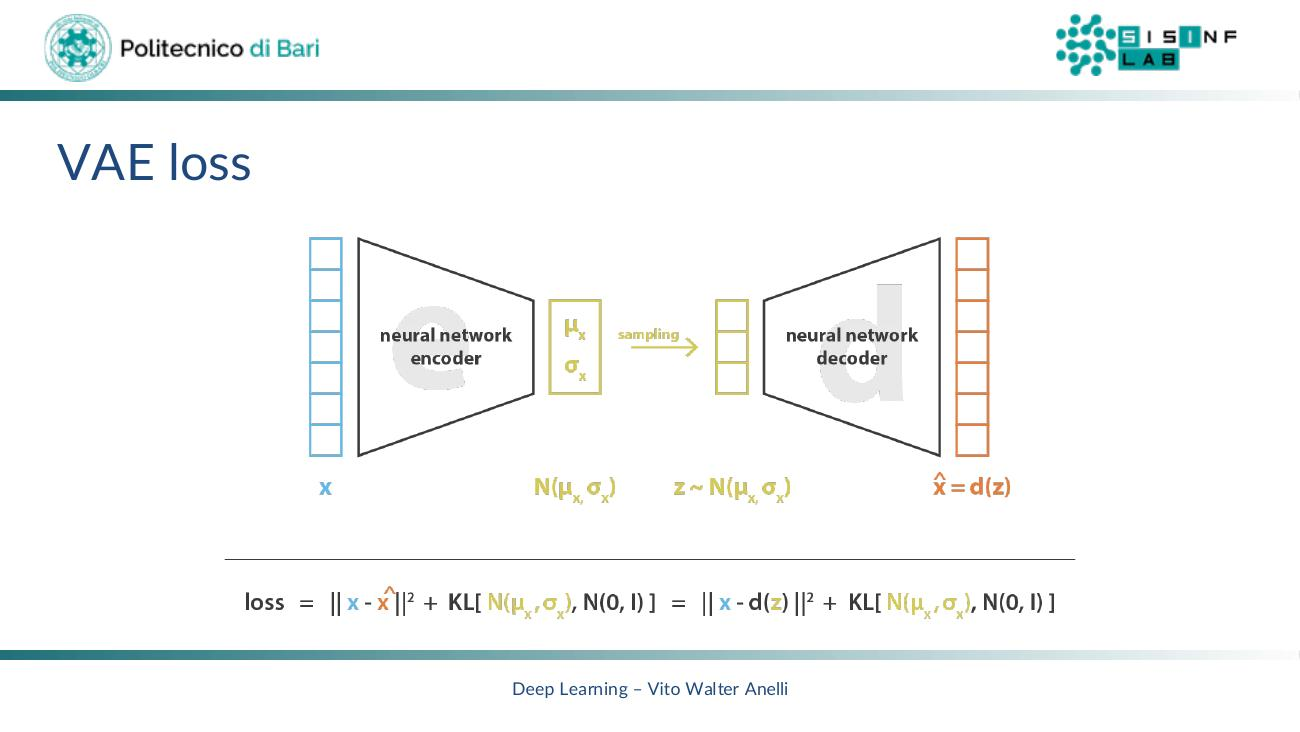
\includegraphics[width=0.82\linewidth]{figures/cf10_vae_loss_diagram.jpg}
  \caption{Schema della loss del VAE. L'encoder produce
           $(\boldsymbol{\mu}_\mathbf{x}, \boldsymbol{\sigma}_\mathbf{x})$;
           un punto $\mathbf{z} \sim \mathcal{N}(\boldsymbol{\mu}_\mathbf{x},
           \boldsymbol{\sigma}_\mathbf{x})$ viene decodificato in
           $\hat{\mathbf{x}} = d(\mathbf{z})$. La loss combina
           errore di ricostruzione e KL-divergenza.}
  \label{fig:vae_loss}
\end{figure}

\subsection{Proprietà dello Spazio Latente Regolarizzato}
\label{subsec:vae-latent-space}

Le due proprietà fondamentali che la regolarizzazione KL impone allo
spazio latente sono:

\begin{description}
  \item[Continuità] Punti vicini nello spazio latente producono output
        simili una volta decodificati.
  \item[Completezza] Qualsiasi punto campionato dalla prior
        $p(\mathbf{z}) = \mathcal{N}(\mathbf{0},\mathbf{I})$ produce un
        output semanticamente significativo.
\end{description}

Senza regolarizzazione, l'encoder potrebbe imparare distribuzioni con
varianza nulla (riducendosi a un autoencoder classico) o con medie molto
distanti tra loro, rendendo lo spazio latente discontinuo e privo di
significato generativo.

\begin{figure}[H]
  \centering
  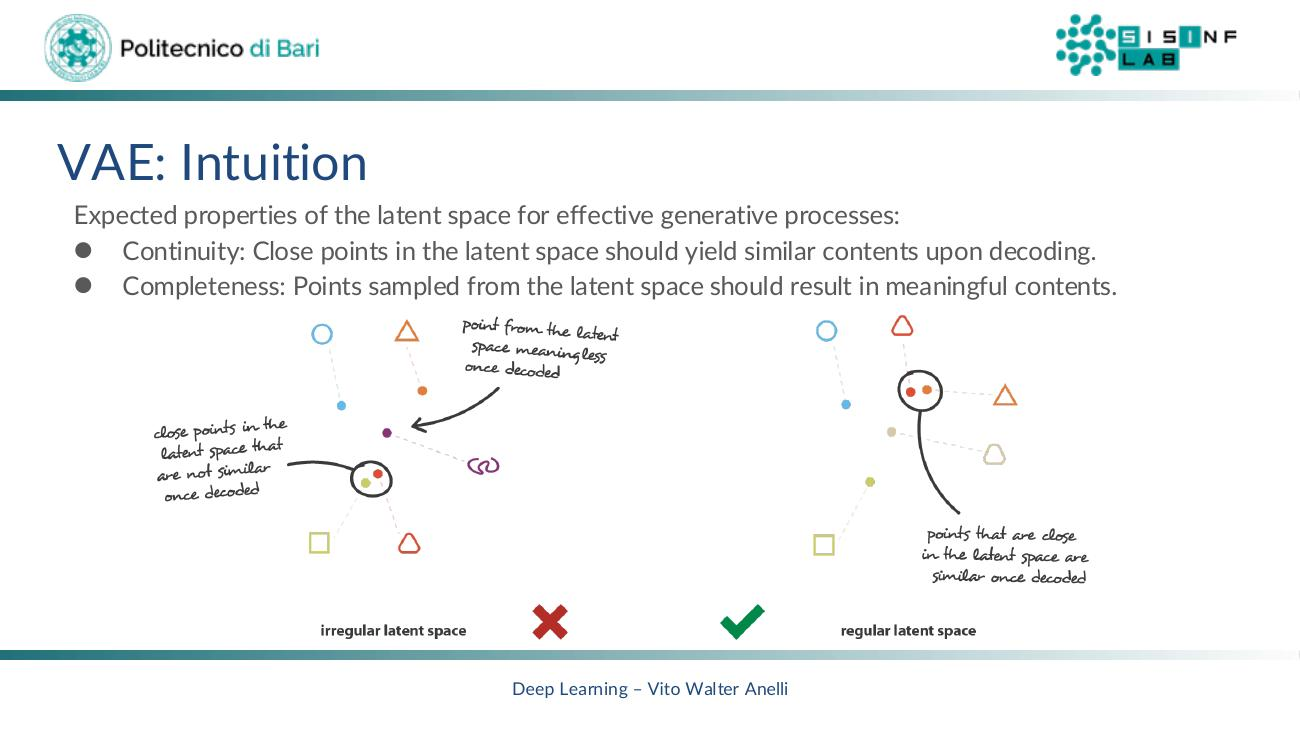
\includegraphics[width=0.82\linewidth]{figures/cf10_vae_latent_space_intuition.jpg}
  \caption{Confronto tra spazio latente irregolare (sinistra, autoencoder
           senza regolarizzazione: punti vicini non simili, regioni vuote)
           e spazio latente regolare (destra, VAE: distribuzioni continue
           e sovrapposte, proprietà di continuità e completezza
           garantite).}
  \label{fig:vae_latent}
\end{figure}

\subsection{Il Reparametrization Trick}
\label{subsec:reparam-trick}

Il campionamento $\mathbf{z} \sim \mathcal{N}(\boldsymbol{\mu}_\mathbf{x},
\boldsymbol{\sigma}_\mathbf{x})$ è un'operazione \emph{stocastica} non
differenziabile; i gradienti non possono fluire attraverso di essa verso i
parametri dell'encoder. Il \textbf{reparametrization trick}
\citep{kingma2014vae} risolve il problema spostando la stocasticità su
una variabile ausiliaria $\boldsymbol{\zeta}$ indipendente dai parametri:

\begin{equation}
  \boldsymbol{\zeta} \sim \mathcal{N}(\mathbf{0}, \mathbf{I}),
  \qquad
  \mathbf{z} = \boldsymbol{\sigma}_\mathbf{x} \odot \boldsymbol{\zeta}
             + \boldsymbol{\mu}_\mathbf{x}.
  \label{eq:reparam}
\end{equation}

Il grafo computazionale risultante è differenziabile rispetto a
$\boldsymbol{\mu}_\mathbf{x}$ e $\boldsymbol{\sigma}_\mathbf{x}$, poiché
il campionamento avviene su $\boldsymbol{\zeta}$, che non dipende dai
parametri della rete.

\begin{figure}[H]
  \centering
  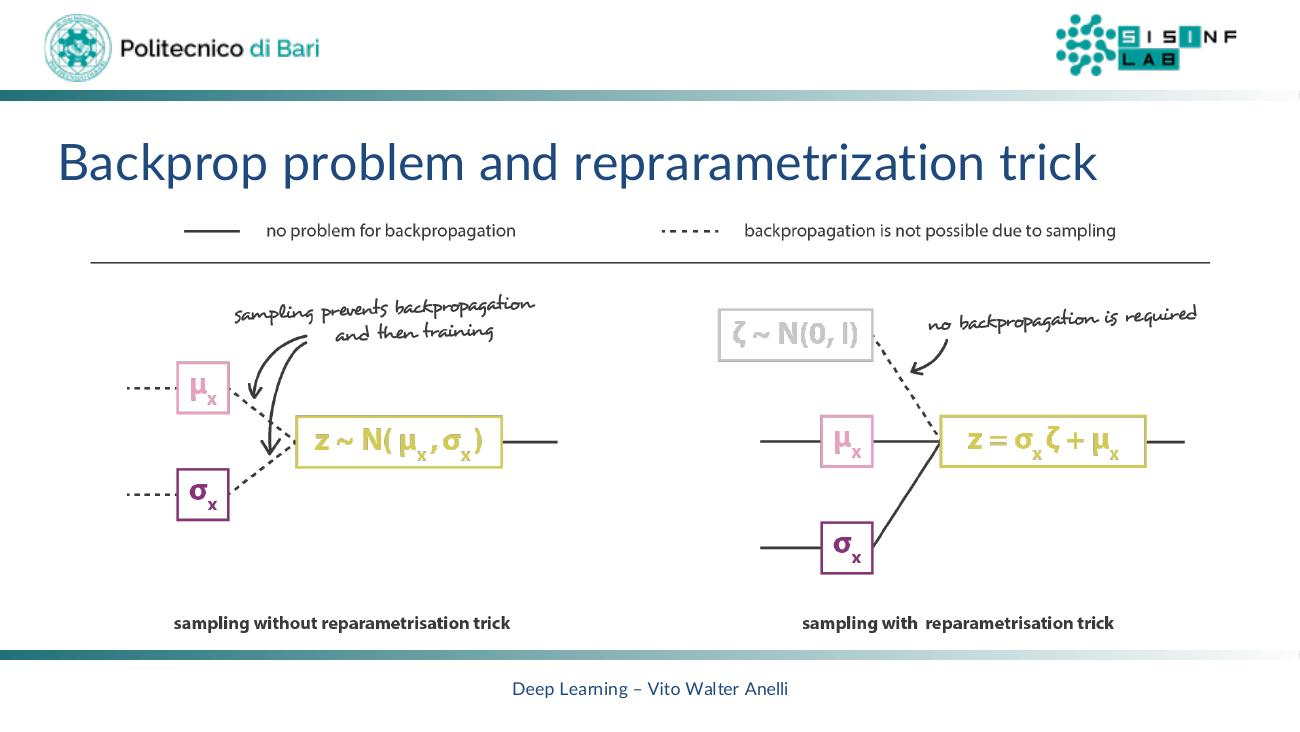
\includegraphics[width=0.82\linewidth]{figures/cf10_vae_reparam_trick.jpg}
  \caption{Reparametrization trick. Sinistra: il campionamento diretto
           $\mathbf{z} \sim \mathcal{N}(\boldsymbol{\mu}_\mathbf{x},
           \boldsymbol{\sigma}_\mathbf{x})$ blocca la backpropagation
           (linee tratteggiate). Destra: con il trick,
           $\boldsymbol{\zeta} \sim \mathcal{N}(\mathbf{0},\mathbf{I})$
           è esterno al grafo, e la trasformazione
           $\mathbf{z} = \boldsymbol{\sigma}_\mathbf{x}\boldsymbol{\zeta}
           + \boldsymbol{\mu}_\mathbf{x}$ è differenziabile (linee
           continue).}
  \label{fig:reparam}
\end{figure}

\subsection{Schema Completo del VAE}
\label{subsec:vae-complete}

\begin{figure}[H]
  \centering
  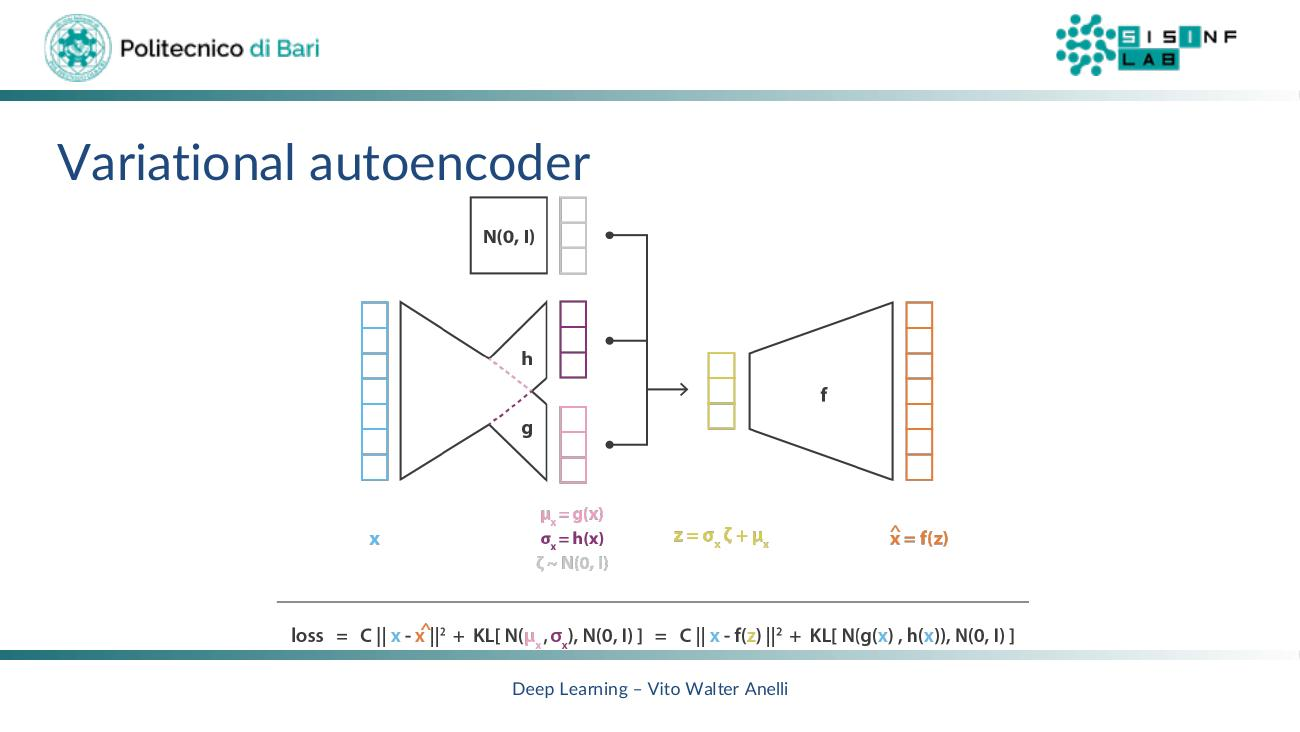
\includegraphics[width=0.88\linewidth]{figures/cf10_vae_full_diagram.jpg}
  \caption{Schema completo del VAE con reparametrization trick. L'encoder
           produce $\boldsymbol{\mu}_\mathbf{x} = g(\mathbf{x})$ e
           $\boldsymbol{\sigma}_\mathbf{x} = h(\mathbf{x})$; il campionamento
           è realizzato tramite $\mathbf{z} = \boldsymbol{\sigma}_\mathbf{x}
           \boldsymbol{\zeta} + \boldsymbol{\mu}_\mathbf{x}$ con
           $\boldsymbol{\zeta} \sim \mathcal{N}(\mathbf{0},\mathbf{I})$;
           il decoder restituisce $\hat{\mathbf{x}} = f(\mathbf{z})$. La loss
           è la somma di errore di ricostruzione e KL-divergenza.}
  \label{fig:vae_full}
\end{figure}

\paragraph{Implementazione in PyTorch.}

\begin{lstlisting}[language=Python, caption={VAE: encoder, reparametrization
  e loss in PyTorch.}, label={lst:vae-pytorch}]
import torch
import torch.nn as nn
import torch.nn.functional as F

class VAE(nn.Module):
    def __init__(self, d_in, d_h, d_z):
        super().__init__()
        # Encoder: produce mu e log-varianza
        self.fc1    = nn.Linear(d_in, d_h)
        self.fc_mu  = nn.Linear(d_h, d_z)
        self.fc_log = nn.Linear(d_h, d_z)
        # Decoder
        self.fc3    = nn.Linear(d_z, d_h)
        self.fc4    = nn.Linear(d_h, d_in)

    def encode(self, x):
        h = F.relu(self.fc1(x))
        return self.fc_mu(h), self.fc_log(h)

    def reparametrize(self, mu, log_var):
        std = torch.exp(0.5 * log_var)
        zeta = torch.randn_like(std)   # N(0,I)
        return mu + std * zeta         # eq. (10.13)

    def decode(self, z):
        h = F.relu(self.fc3(z))
        return torch.sigmoid(self.fc4(h))

    def forward(self, x):
        mu, log_var = self.encode(x)
        z = self.reparametrize(mu, log_var)
        x_hat = self.decode(z)
        return x_hat, mu, log_var

def vae_loss(x_hat, x, mu, log_var):
    rec = F.mse_loss(x_hat, x, reduction="sum")
    kl  = -0.5 * torch.sum(
              1 + log_var - mu.pow(2) - log_var.exp())
    return rec + kl
\end{lstlisting}

%------------------------------------------------------------
\section{Confronto e Riepilogo}
\label{sec:ae-summary}

\begin{table}[H]
  \centering
  \caption{Confronto tra le varianti di autoencoder trattate.}
  \label{tab:ae-comparison}
  \small
  \begin{tabular}{lllll}
    \toprule
    \textbf{Modello} & \textbf{Vincolo} & \textbf{Spazio latente}
      & \textbf{Generativo} & \textbf{Applicazione tipica} \\
    \midrule
    AE classico & $k < d$ & Punto & No & Compressione, pre-training \\
    Sparse AE   & $\ell_1$ su $\mathbf{a}$ & Punto sparso & No &
      Feature learning \\
    Deep AE     & Più livelli & Punto profondo & No &
      Compressione non lineare \\
    U-Net       & Skip connections & --- & No &
      Segmentazione semantica \\
    VAE         & KL$(\cdot\|\mathcal{N}(\mathbf{0},\mathbf{I}))$ &
      Distribuzione & Sì & Generazione, interpolazione \\
    \bottomrule
  \end{tabular}
\end{table}

\paragraph{Linee guida pratiche.}
\begin{enumerate}
  \item Per \textbf{compressione} o \textbf{riduzione dimensionale}:
        usare un deep autoencoder con tied weights; la dimensione del
        collo di bottiglia è un iperparametro da cercare tramite
        validation.
  \item Per \textbf{feature learning} non supervisionato: preferire lo
        sparse autoencoder (o un denoising autoencoder, che aggiunge
        rumore all'input e lo richiede pulito all'uscita).
  \item Per \textbf{segmentazione semantica pixel-per-pixel}: usare la
        U-Net con skip connections; la scelta della profondità ($n$ livelli
        di pooling) dipende dalla risoluzione dell'immagine.
  \item Per \textbf{generazione} e \textbf{interpolazione nello spazio
        latente}: usare un VAE; il bilanciamento tra termine di
        ricostruzione e termine KL (tramite un iperparametro $\beta$,
        come nel $\beta$-VAE) controlla il trade-off tra qualità
        ricostruttiva e regolarità dello spazio latente.
  \item Ricordare il reparametrization trick: senza di esso la
        backpropagation non attraversa il nodo di campionamento e
        l'addestramento del VAE non converge.
\end{enumerate}

Come sottolinea \citet{bishop2024}, gli autoencoder rappresentano un
paradigma fondamentale dell'apprendimento non supervisionato: la
successione AE $\to$ Sparse AE $\to$ Denoising AE $\to$ VAE traccia
un percorso verso modelli generativi sempre più strutturati, che
costituisce la base concettuale dei modelli di diffusione moderni.
%============================================================
%  Capitolo 11 – Generative Adversarial Networks
%============================================================
\chapter{Generative Adversarial Networks}
\label{ch:gans}

Le \textbf{Generative Adversarial Networks} (GAN) sono un framework di
apprendimento generativo proposto da Goodfellow et al.\ nel 2014 in cui
due reti neurali --- un \emph{generatore} e un \emph{discriminatore} ---
vengono addestrate simultaneamente in un regime di competizione.
L'idea fondamentale consiste nel sostituire la comparazione diretta tra
distribuzioni di probabilità con un \emph{task} di discriminazione
indiretto, che spinge il generatore a produrre campioni sempre più
indistinguibili dai dati reali \citep{bishop2024}.

%------------------------------------------------------------
\section{Preliminari: Variabili Aleatorie e Modelli Generativi}
\label{sec:gan-preliminaries}

\subsection{Generazione di Variabili Aleatorie}
\label{subsec:rand-vars}

Il processo di generazione di variabili aleatorie complesse parte dalla
constatazione che i calcolatori sono deterministici: non è possibile
produrre vera casualità, ma algoritmi \emph{pseudorandom} consentono di
generare sequenze di numeri con proprietà statisticamente molto vicine
a quelle di una distribuzione uniforme nell'intervallo $[0,1]$.

A partire da queste variabili uniformi si possono ottenere distribuzioni
più complesse attraverso diverse tecniche:

\begin{description}
  \item[Inverse Transform Method] L'idea è di estendere il metodo
        dell'inversa della CDF a una nozione più generale di
        \emph{transform method}: si genera una variabile casuale come
        funzione di variabili più semplici (non necessariamente uniformi).
        La funzione di trasformazione \emph{deforma} la distribuzione
        iniziale, sottraendo massa dove la distribuzione di partenza è
        troppo alta rispetto al target e aggiungendola dove è troppo
        bassa.
  \item[Rejection Sampling] Si campiona da una distribuzione
        proponente più semplice e si accetta o rifiuta il campione in
        base a un criterio probabilistico.
  \item[Metropolis-Hastings] Algoritmo MCMC che costruisce una catena
        di Markov la cui distribuzione stazionaria coincide con la
        distribuzione target.
\end{description}

\subsection{Modelli Generativi}
\label{subsec:generative-models}

Si consideri il problema di generare immagini in bianco e nero di
dimensione $n \times n$ pixel. Ogni immagine può essere rappresentata
come un vettore $\mathbf{x} \in \mathbb{R}^N$ con $N = n^2$ (i pixel
vengono appiattiti colonna per colonna). Le immagini che
\emph{assomigliano} a una certa categoria (es.\ cani) non sono
distribuite uniformemente nello spazio $\mathbb{R}^N$: esiste una
distribuzione di probabilità specifica, molto complessa e ad alta
dimensionalità, che assegna alta probabilità ai vettori corrispondenti
a cani realistici e bassa probabilità agli altri.

Questo implica due osservazioni fondamentali:

\begin{enumerate}
  \item La distribuzione target è \textbf{molto complessa} e definita
        su uno spazio ad altissima dimensionalità.
  \item Anche se possiamo assumerne l'esistenza, \textbf{non sappiamo
        come esprimerla esplicitamente}.
\end{enumerate}

Generare una nuova immagine di un cane è quindi equivalente al problema
di campionare un nuovo vettore che segua la distribuzione target.
L'approccio con reti neurali consiste nel modellare questa distribuzione
implicitamente attraverso una \textbf{rete generativa}: la rete riceve
in input variabili aleatorie semplici (ad esempio uniformi o gaussiane)
e produce in output un campione distribuito (dopo l'addestramento)
secondo la distribuzione target.

\begin{figure}[H]
  \centering
  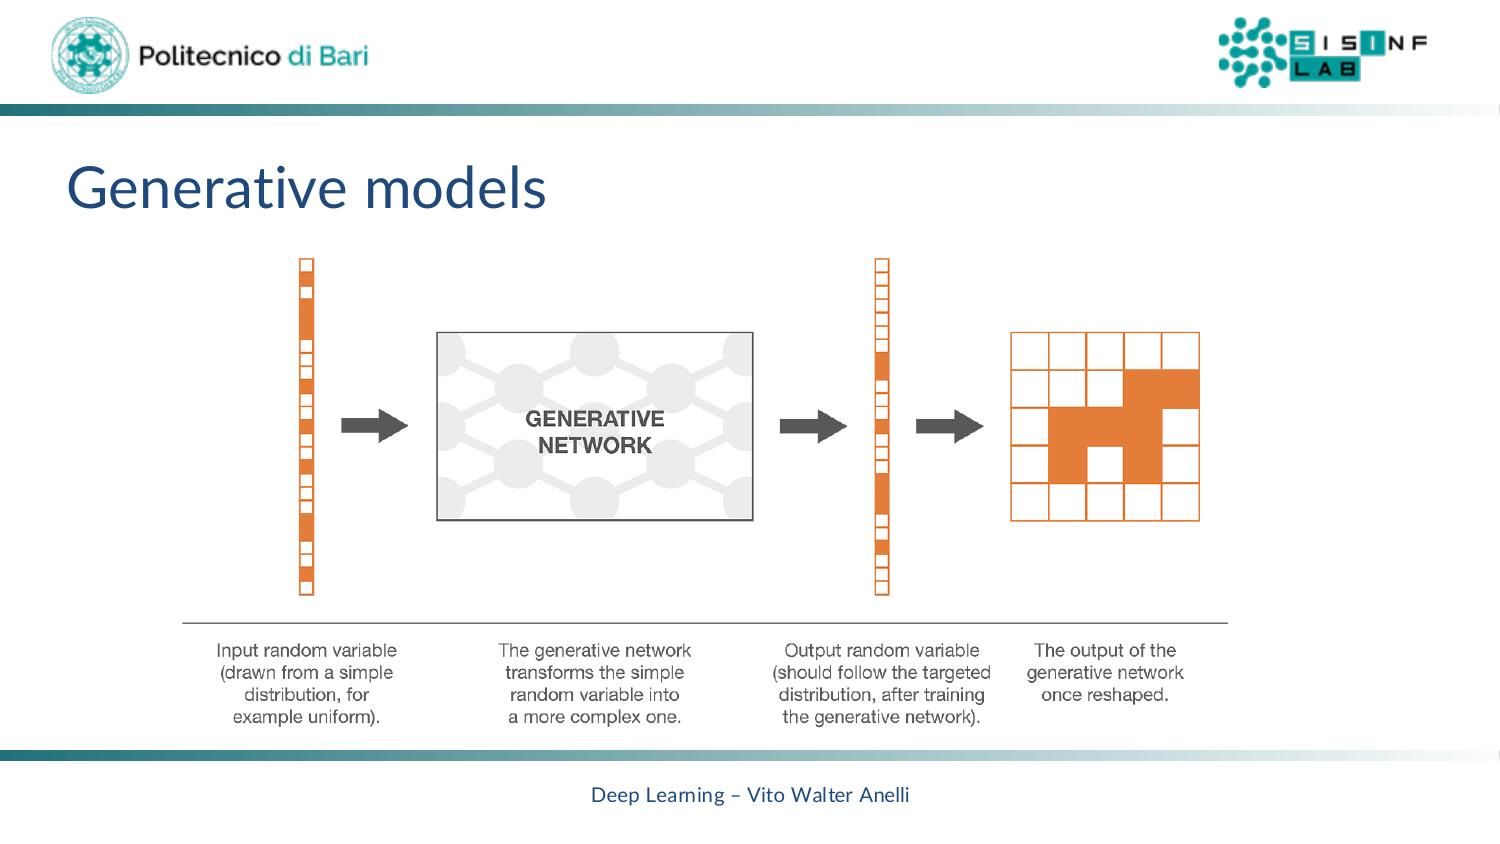
\includegraphics[width=0.82\linewidth]{figures/cf11_gan_generative_model.jpg}
  \caption{Schema di una rete generativa. Una variabile casuale campionata
           da una distribuzione semplice (uniforme) viene trasformata
           dalla rete in un vettore ad alta dimensionalità che, una volta
           ridimensionato a matrice, produce un'immagine sintetica. Dopo
           l'addestramento, la distribuzione dell'output deve coincidere
           con la distribuzione target.}
  \label{fig:gan_generative_model}
\end{figure}

\subsubsection{Addestramento Diretto}

L'approccio ``diretto'' consiste nel ripetere iterativamente i seguenti
passi:

\begin{enumerate}
  \item Campionare alcuni input uniformi $\mathbf{z}$.
  \item Propagarli attraverso la rete e raccogliere gli output generati
        $\mathbf{x}' = G(\mathbf{z})$.
  \item Confrontare la distribuzione generata con quella reale usando una
        metrica campionaria (es.\ la \emph{Maximum Mean Discrepancy},
        MMD).
  \item Eseguire un passo di discesa del gradiente per ridurre la
        distanza tra le due distribuzioni.
\end{enumerate}

\begin{figure}[H]
  \centering
  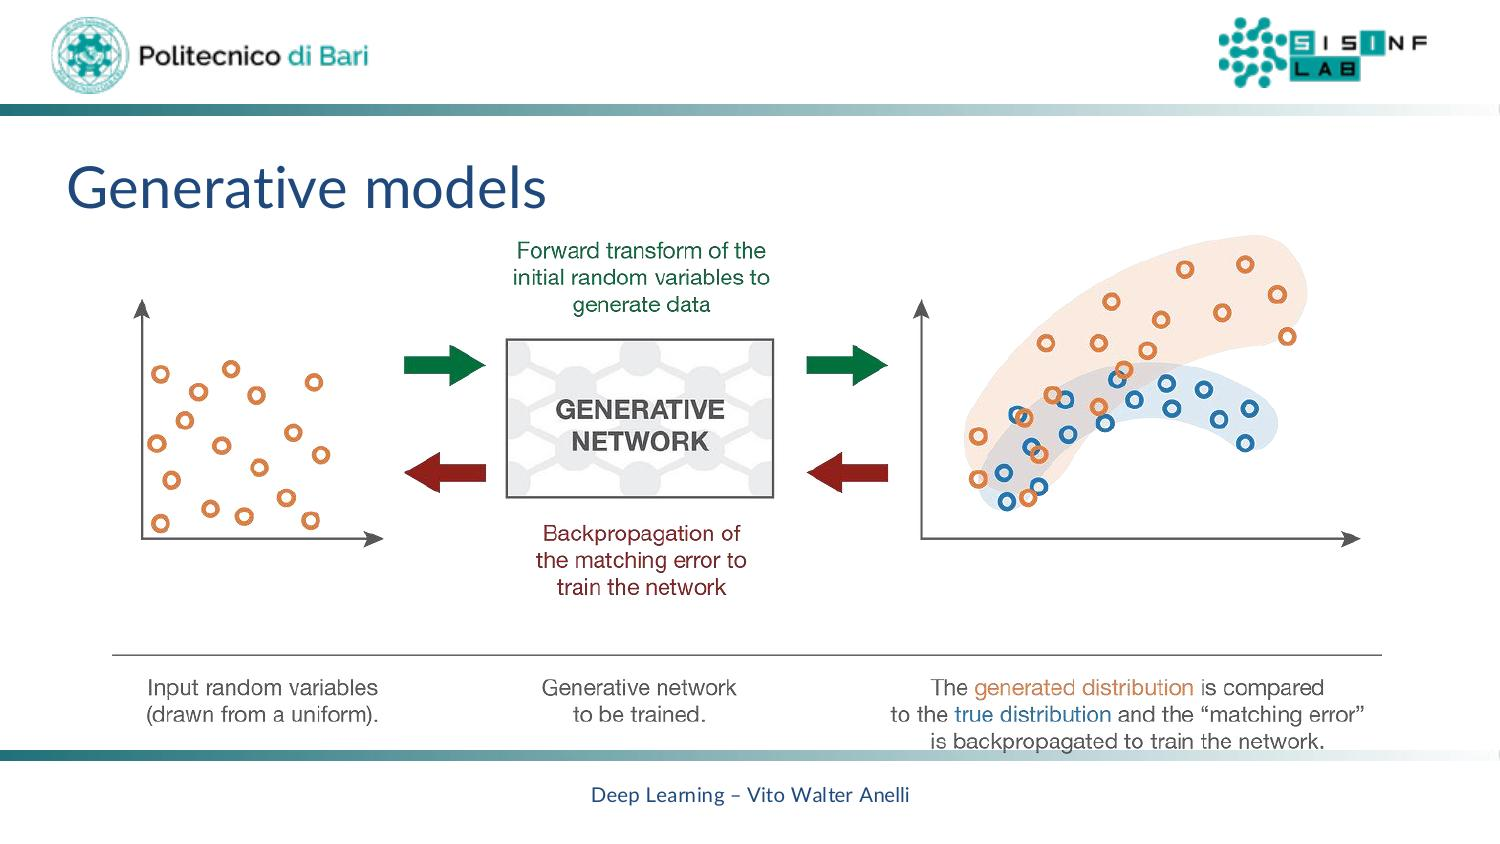
\includegraphics[width=0.82\linewidth]{figures/cf11_gan_training_loop.jpg}
  \caption{Schema dell'addestramento diretto di una rete generativa.
           La distribuzione generata (arancione) viene confrontata con
           quella reale (blu) e l'errore di corrispondenza viene
           retropropagato per aggiornare i pesi della rete.}
  \label{fig:gan_training_loop}
\end{figure}

La difficoltà principale di questo approccio è che il confronto diretto
tra distribuzioni di probabilità a partire da campioni è
computazionalmente costoso e spesso mal condizionato in alta dimensione.
Le GAN propongono una soluzione elegante a questo problema.

%------------------------------------------------------------
\section{Generative Adversarial Networks}
\label{sec:gan-core}

\subsection{L'Idea Fondamentale: Confronto Indiretto}
\label{subsec:gan-idea}

La brillante intuizione alla base delle GAN consiste nel rimpiazzare
il confronto diretto tra distribuzioni con uno \textbf{indiretto}, che
assume la forma di un task a valle (\emph{downstream task}) di
discriminazione tra campioni reali e campioni generati. L'addestramento
del generatore viene svolto rispetto a questo task in modo tale che la
distribuzione generata venga spinta progressivamente verso quella reale
\citep{bishop2024}.

Il task a valle è un \textbf{problema di classificazione binaria}: dato
un campione, determinare se esso proviene dalla distribuzione reale
(``vero'') o dal generatore (``falso''). Dal punto di vista del
generatore, si tratta di un task di \emph{non-discriminazione}: si
vuole che la classificazione fallisca il più possibile.

\subsection{Architettura GAN}
\label{subsec:gan-arch}

In un'architettura GAN sono presenti due reti:

\begin{description}
  \item[Generatore $G$] Rete neurale che modella una funzione di
        trasformazione. Riceve in input una variabile latente
        $\mathbf{z} \in \mathbb{R}^d$ campionata da una distribuzione
        semplice (tipicamente $\mathbf{z} \sim \mathcal{N}(\mathbf{0},
        \mathbf{I})$) e produce un campione sintetico
        $\mathbf{x}' = G(\mathbf{z})$.
        L'obiettivo, una volta addestrato, è che $\mathbf{x}'$ segua
        la distribuzione target.
  \item[Discriminatore $D$] Rete neurale che modella una funzione
        discriminativa. Riceve in input un punto $\mathbf{x}$ (vettore
        $N$-dimensionale) e restituisce la probabilità stimata che tale
        punto provenga dalla distribuzione reale:
        $D(\mathbf{x}) \in [0, 1]$.
\end{description}

Le due reti vengono addestrate \textbf{congiuntamente} con obiettivi
opposti:

\begin{itemize}
  \item Il generatore cerca di \emph{ingannare} il discriminatore, ossia
        è addestrato a \textbf{massimizzare} l'errore di classificazione
        (gradiente ascendente sull'errore rispetto ai parametri di $G$).
  \item Il discriminatore cerca di \emph{rilevare} i campioni falsi,
        ossia è addestrato a \textbf{minimizzare} l'errore di
        classificazione (discesa del gradiente rispetto ai parametri
        di $D$).
\end{itemize}

\begin{figure}[H]
  \centering
  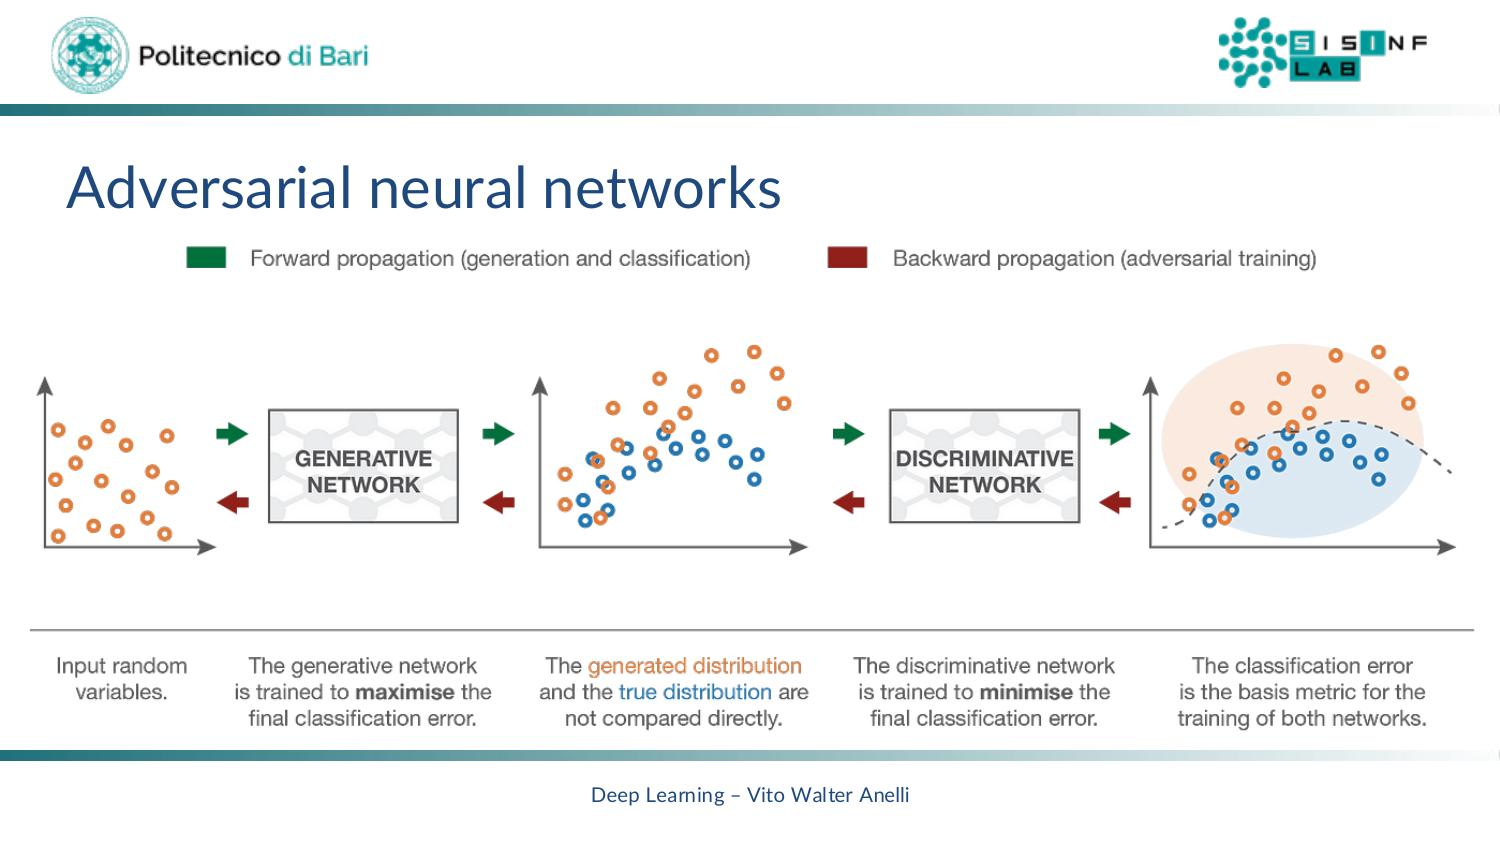
\includegraphics[width=0.95\linewidth]{figures/cf11_gan_adversarial_arch.jpg}
  \caption{Architettura adversariale. La rete generativa (sinistra)
           trasforma variabili casuali in campioni sintetici; la rete
           discriminativa (destra) riceve campioni reali e generati e
           tenta di classificarli correttamente. Le frecce rosse
           rappresentano la backpropagation avversariale: il generatore
           è addestrato a massimizzare l'errore di classificazione,
           il discriminatore a minimizzarlo.}
  \label{fig:gan_adversarial_arch}
\end{figure}

\subsection{Architettura Pratica}
\label{subsec:gan-practical-arch}

\begin{figure}[H]
  \centering
  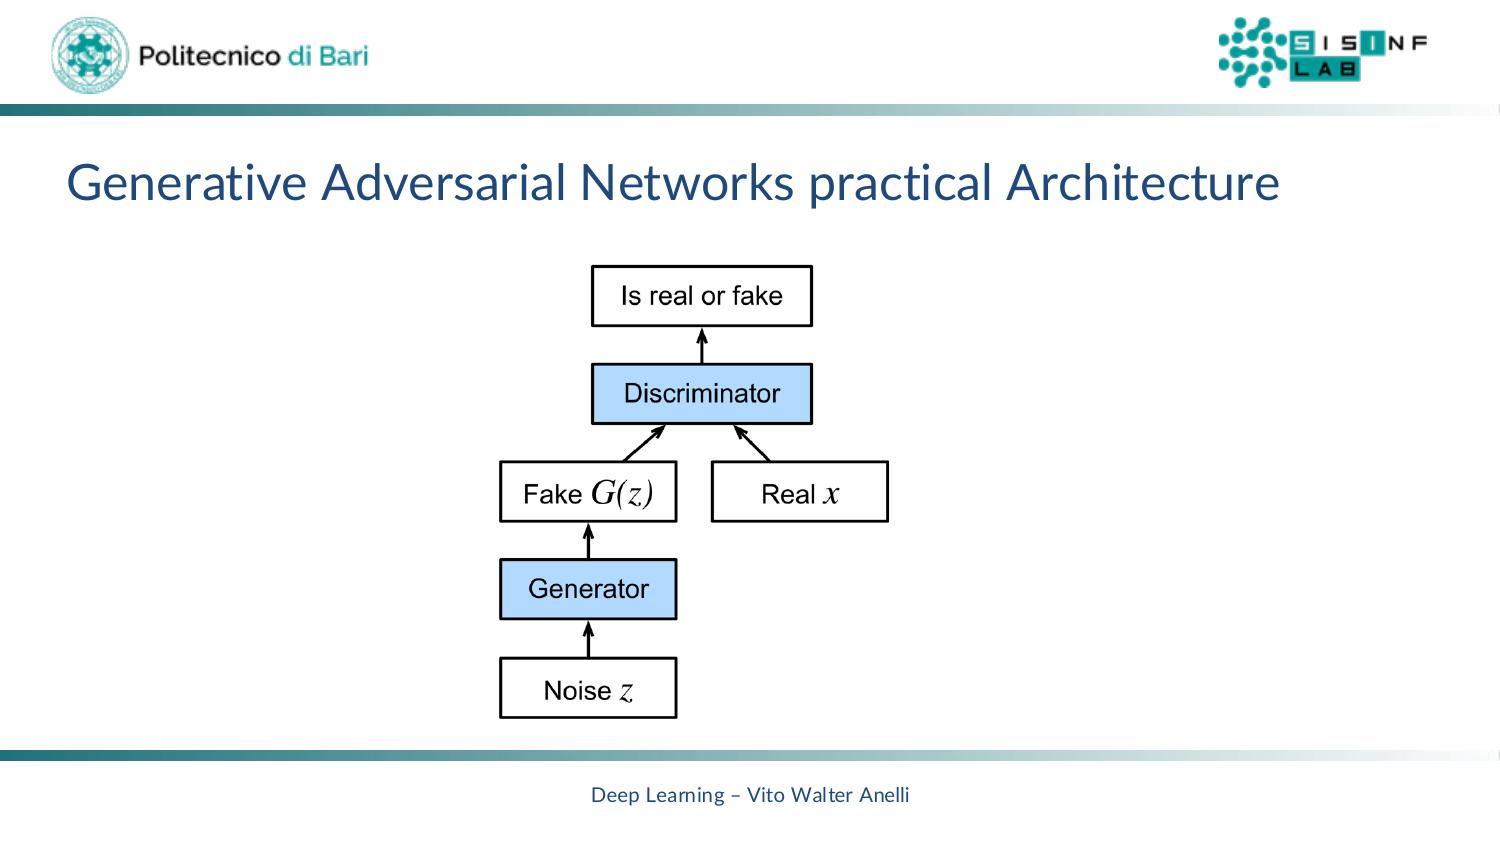
\includegraphics[width=0.60\linewidth]{figures/cf11_gan_practical_arch.jpg}
  \caption{Architettura GAN pratica. Il generatore riceve il rumore
           $\mathbf{z}$ e produce $G(\mathbf{z})$ (campione falso). Il
           discriminatore riceve sia i campioni reali $\mathbf{x}$ che
           quelli falsi $G(\mathbf{z})$ e produce una predizione scalare
           (\emph{reale} o \emph{falso}).}
  \label{fig:gan_practical_arch}
\end{figure}

%------------------------------------------------------------
\section{Formulazione Matematica}
\label{sec:gan-math}

\subsection{Loss del Discriminatore}
\label{subsec:gan-loss-disc}

Il discriminatore è un classificatore binario. L'output è una
probabilità scalare $D(\mathbf{x}) = 1/(1 + e^{-o})$, dove $o$ è
l'uscita pre-sigmoid (tipicamente uno strato completamente connesso con
dimensione nascosta 1). Le etichette sono $y = 1$ per i dati reali e
$y = 0$ per quelli generati. La loss del discriminatore è la
\textbf{cross-entropy binaria}:

\begin{equation}
  \mathcal{L}_D = \min_{D}
    \Bigl\{-y \log D(\mathbf{x}) - (1 - y)\log(1 - D(\mathbf{x}))\Bigr\}.
  \label{eq:gan-disc-loss}
\end{equation}

Espandendo sulle due classi separatamente:

\begin{align}
  \mathcal{L}_D &= \min_{D}
    \Bigl\{-\mathbb{E}_{x \sim p_{\text{data}}} \log D(\mathbf{x})
           -\mathbb{E}_{z \sim p_z} \log(1 - D(G(\mathbf{z})))\Bigr\}.
  \label{eq:gan-disc-loss-expanded}
\end{align}

\subsection{Loss del Generatore}
\label{subsec:gan-loss-gen}

Per un dato discriminatore $D$, il generatore $G$ viene aggiornato per
massimizzare la cross-entropy loss quando $y = 0$, ovvero:

\begin{equation}
  \max_{G}\bigl\{-(1-y)\log(1 - D(G(\mathbf{z})))\bigr\}
    = \max_{G}\bigl\{-\log(1 - D(G(\mathbf{z})))\bigr\}.
  \label{eq:gan-gen-loss-orig}
\end{equation}

Tuttavia, quando il generatore produce campioni di qualità
($D(G(\mathbf{z})) \approx 1$), la funzione
$-\log(1 - D(G(\mathbf{z})))$ tende a zero e i gradienti risultano
troppo piccoli per fare progressi efficaci. Si preferisce quindi
minimizzare la seguente loss equivalente (con i target etichettati come
se fossero reali, $y = 1$):

\begin{equation}
  \min_{G}\bigl\{\log(1 - D(G(\mathbf{z})))\bigr\}
    \approx \max_{G}\bigl\{-\log(D(G(\mathbf{z})))\bigr\}.
  \label{eq:gan-gen-loss-flip}
\end{equation}

Questa formulazione (\emph{non-saturating GAN loss}) ha gradienti
significativi anche nelle prime fasi dell'addestramento, quando il
discriminatore riesce facilmente a distinguere campioni reali da falsi.

\subsection{Obiettivo Minimax Complessivo}
\label{subsec:gan-minimax}

Unificando le due loss, $D$ e $G$ giocano un gioco minimax a due
giocatori con la seguente funzione obiettivo:

\begin{equation}
  \min_{D}\max_{G}
    \Bigl\{-\mathbb{E}_{x \sim p_{\text{data}}} \log D(\mathbf{x})
           -\mathbb{E}_{z \sim p_z} \log(1 - D(G(\mathbf{z})))\Bigr\}.
  \label{eq:gan-minimax}
\end{equation}

\begin{figure}[H]
  \centering
  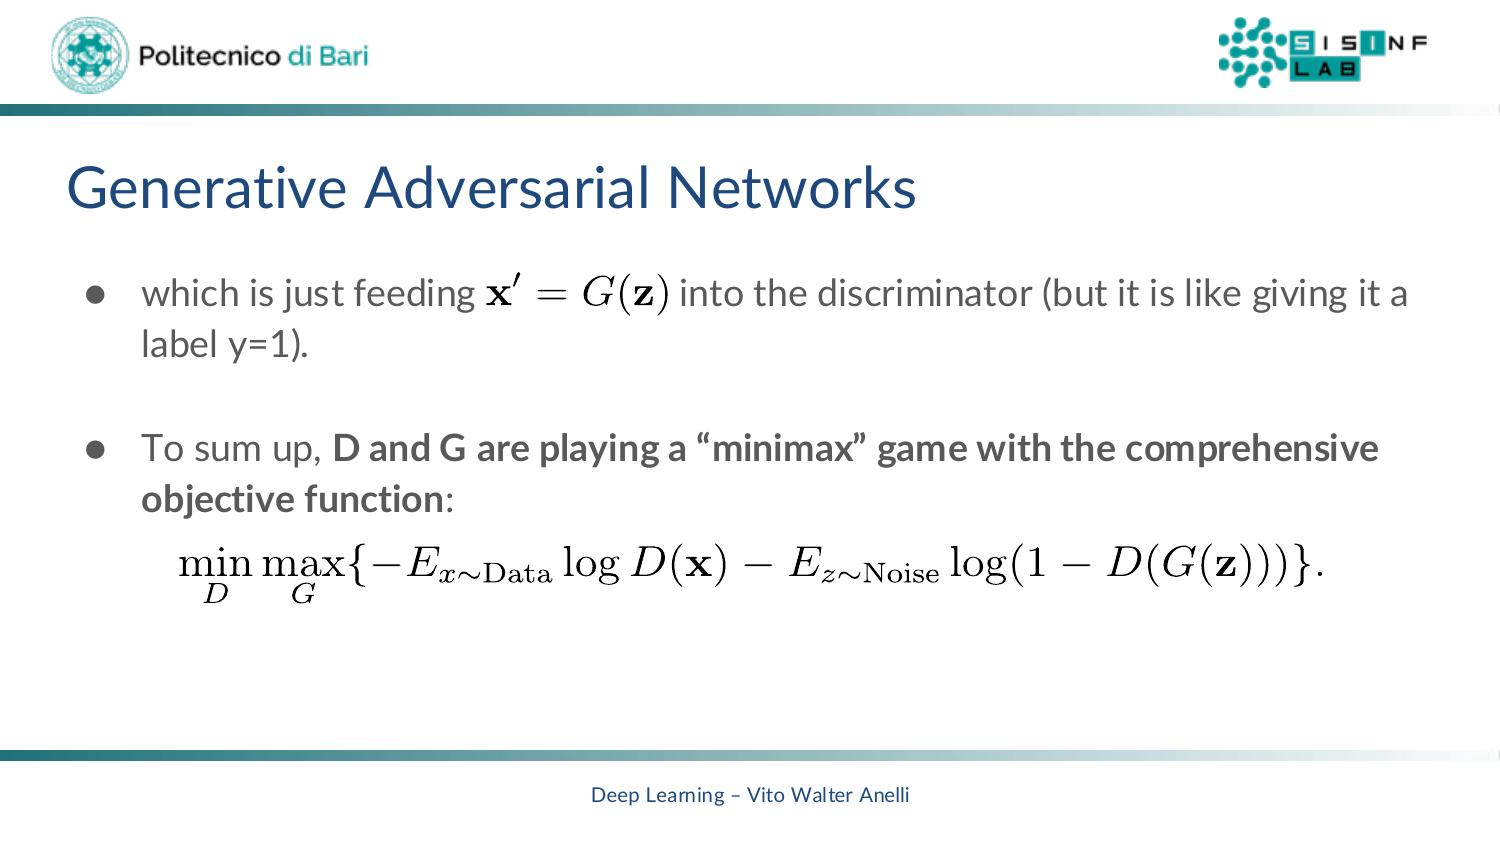
\includegraphics[width=0.82\linewidth]{figures/cf11_gan_minimax.jpg}
  \caption{Obiettivo minimax della GAN. Il discriminatore $D$ minimizza
           la cross-entropy binaria; il generatore $G$ la massimizza
           alimentando campioni falsi $G(\mathbf{z})$ nel discriminatore
           come se fossero reali ($y = 1$).}
  \label{fig:gan_minimax}
\end{figure}

\subsection{Interpretazione Game-Theoretic}
\label{subsec:gan-game-theory}

Dal punto di vista della teoria dei giochi, questa formulazione
corrisponde a un \textbf{gioco minimax a due giocatori}. Lo stato di
equilibrio (equilibrio di Nash) è raggiunto quando:

\begin{itemize}
  \item Il generatore produce campioni dalla distribuzione target esatta:
        $p_G = p_{\text{data}}$.
  \item Il discriminatore non riesce a fare meglio di una classificazione
        casuale: $D(\mathbf{x}) = 1/2$ per ogni punto $\mathbf{x}$.
\end{itemize}

Si può dimostrare che, a questo equilibrio, l'obiettivo minimax
equivale a minimizzare la \textbf{Jensen-Shannon Divergence} (JSD) tra
$p_{\text{data}}$ e $p_G$ \citep{bishop2024}:

\begin{equation}
  \mathcal{L}^* = -2\log 2
    + 2 \cdot \mathrm{JSD}(p_{\text{data}} \| p_G).
  \label{eq:gan-jsd}
\end{equation}

L'obiettivo è quindi minimizzare la JSD, che è zero se e solo se
$p_G = p_{\text{data}}$.

%------------------------------------------------------------
\section{Dinamica dell'Addestramento}
\label{sec:gan-training}

\subsection{Il Caso Ideale: Discriminatore Oracolo}
\label{subsec:gan-ideal-case}

Per comprendere la dinamica adversariale si consideri il caso
monodimensionale in cui la distribuzione target è una gaussiana
$\mathcal{N}(\mu, \sigma^2)$ e il generatore produce campioni da
un'altra gaussiana con parametri diversi.

Nell'approccio diretto, il generatore viene aggiornato
iterativamente correggendo la differenza misurata tra le due
distribuzioni fino a convergenza. Con un discriminatore oracolo (che
conosce esattamente le due distribuzioni), il gradiente fornito al
generatore è proporzionale alla differenza puntuale tra le densità.
Man mano che le due gaussiane si avvicinano, il discriminatore fatica
sempre di più a distinguerle, e all'equilibrio --- quando le
distribuzioni coincidono --- la sua accuratezza degrada a $50\%$.

\begin{figure}[H]
  \centering
  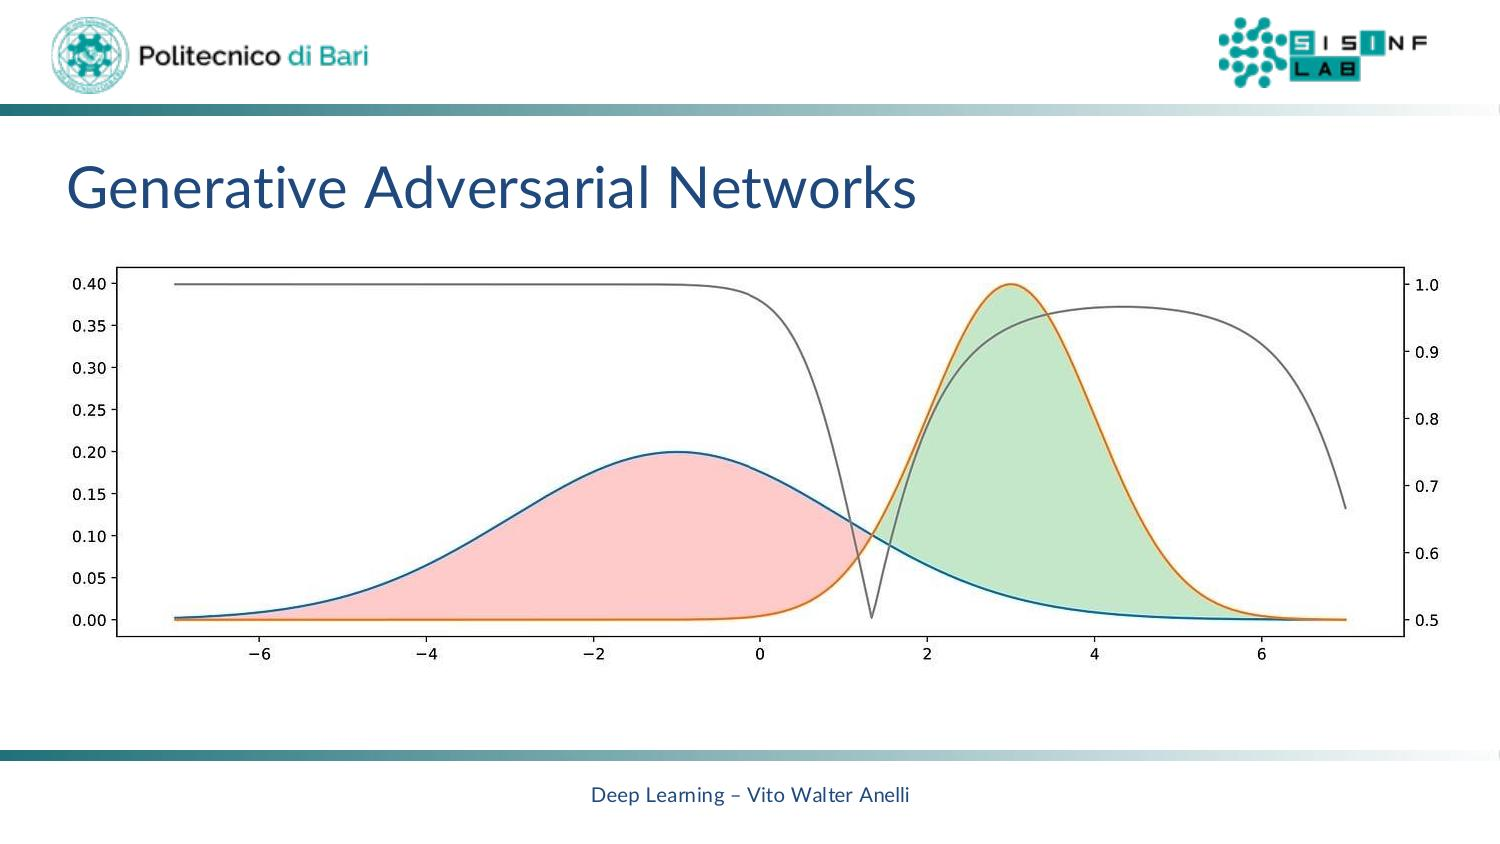
\includegraphics[width=0.82\linewidth]{figures/cf11_gan_discriminator_viz.jpg}
  \caption{Visualizzazione della dinamica discriminatore--generatore.
           In blu: distribuzione reale; in arancione: distribuzione
           generata. In grigio (asse destro): probabilità predetta dal
           discriminatore oracolo. L'area rossa indica le regioni in
           cui la distribuzione generata è in eccesso rispetto alla
           reale (da ridurre); l'area verde le regioni in difetto (da
           aumentare). Quanto più le due distribuzioni si sovrappongono,
           tanto più spesso il discriminatore commette errori.}
  \label{fig:gan_discriminator_viz}
\end{figure}

\subsection{L'Approssimazione Pratica: Reti Neurali}
\label{subsec:gan-approx}

Nella pratica, né il generatore né il discriminatore sono oracoli:
entrambi vengono approssimati con reti neurali e addestrati
congiuntamente. Ad ogni iterazione del ciclo di addestramento:

\begin{enumerate}
  \item I pesi della rete generativa vengono aggiornati in direzione di
        \textbf{ascesa del gradiente} rispetto all'errore di
        classificazione (i.e., $G$ cerca di aumentare l'errore).
  \item I pesi della rete discriminativa vengono aggiornati in direzione
        di \textbf{discesa del gradiente} rispetto allo stesso errore
        (i.e., $D$ cerca di ridurre l'errore).
\end{enumerate}

In questo modo entrambe le reti ``progrediscono'' rispetto ai propri
obiettivi, migliorandosi a vicenda: il discriminatore più capace spinge
il generatore a produrre campioni migliori; il generatore più convincente
costringe il discriminatore a diventare più selettivo. Questo meccanismo
di co-evoluzione dà il nome di \emph{adversarial training}.

\subsection{Procedura di Addestramento}
\label{subsec:gan-training-procedure}

L'algoritmo di addestramento alterna aggiornamenti del discriminatore e
del generatore. Nella formulazione originale \citep{bishop2024}:

\begin{enumerate}
  \item \textbf{Aggiornamento del Discriminatore} (k passi):
        \begin{enumerate}
          \item Campionare un mini-batch di dati reali
                $\{\mathbf{x}^{(i)}\}_{i=1}^{m}$ da $p_{\text{data}}$.
          \item Campionare un mini-batch di rumore latente
                $\{\mathbf{z}^{(i)}\}_{i=1}^{m}$ da $p_z$.
          \item Aggiornare $D$ con discesa del gradiente stocastica:
                \[
                  \nabla_{\theta_D} \frac{1}{m} \sum_{i=1}^{m}
                  \Bigl[\log D(\mathbf{x}^{(i)})
                       + \log\bigl(1 - D(G(\mathbf{z}^{(i)}))\bigr)\Bigr].
                \]
        \end{enumerate}
  \item \textbf{Aggiornamento del Generatore} (1 passo):
        \begin{enumerate}
          \item Campionare un mini-batch di rumore latente
                $\{\mathbf{z}^{(i)}\}_{i=1}^{m}$ da $p_z$.
          \item Aggiornare $G$ con ascesa del gradiente stocastica:
                \[
                  \nabla_{\theta_G} \frac{1}{m} \sum_{i=1}^{m}
                  \log\bigl(D(G(\mathbf{z}^{(i)}))\bigr).
                \]
        \end{enumerate}
\end{enumerate}

Nella pratica, il discriminatore viene tipicamente aggiornato più volte
per ogni aggiornamento del generatore ($k > 1$), in modo da mantenere
il discriminatore ``più forte'' del generatore e fornire un segnale di
gradiente più informativo.

%------------------------------------------------------------
\section{Problematiche nell'Addestramento delle GAN}
\label{sec:gan-issues}

Nonostante l'eleganza teorica, l'addestramento delle GAN presenta
diverse difficoltà pratiche note.

\subsection{Mode Collapse}
\label{subsec:mode-collapse}

Il \textbf{mode collapse} si verifica quando il generatore impara a
produrre solo un sottoinsieme limitato di modi della distribuzione
target, ignorando la varietà presente nei dati reali. In casi estremi,
$G$ converge a produrre sempre lo stesso campione (o pochi campioni
simili), perché questo inganna sistematicamente il discriminatore.
Dal punto di vista della JSD, il mode collapse corrisponde a una
situazione in cui $p_G$ ha supporto molto più piccolo di
$p_{\text{data}}$.

\subsection{Instabilità dell'Addestramento}
\label{subsec:training-instability}

L'equilibrio di Nash del gioco minimax è difficile da raggiungere con
la discesa del gradiente stocastica, perché i gradienti dei due
giocatori interferiscono reciprocamente. Fenomeni tipici sono:

\begin{itemize}
  \item \textbf{Oscillazioni}: generatore e discriminatore non
        convergono ma oscillano in modo ciclico.
  \item \textbf{Vanishing gradients}: se il discriminatore diventa
        troppo forte, $D(G(\mathbf{z})) \approx 0$ e il gradiente
        verso $G$ svanisce.
  \item \textbf{Exploding gradients}: in alcune configurazioni di
        architettura, i gradienti esplodono.
\end{itemize}

\subsection{Soluzioni Proposte}
\label{subsec:gan-solutions}

Diverse varianti architetturali e algoritmiche sono state proposte per
mitigare queste problematiche:

\begin{description}
  \item[Wasserstein GAN (WGAN)] Sostituisce la JSD con la
        \emph{Wasserstein distance} (distanza di Earth Mover), che
        fornisce gradienti più stabili anche quando le distribuzioni
        hanno supporti disgiunti. Richiede il clipping dei pesi del
        discriminatore (o il \emph{gradient penalty}) per soddisfare
        il vincolo di Lipschitz.
  \item[DCGAN] Utilizza convoluzioni nel generatore e nel
        discriminatore, con batch normalization e funzioni di
        attivazione specifiche (ReLU nel generatore, LeakyReLU nel
        discriminatore), migliorando la stabilità su dati visivi.
  \item[Conditional GAN (cGAN)] Condiziona sia il generatore che il
        discriminatore su un'etichetta di classe $y$, permettendo la
        generazione controllata di campioni di una categoria specifica.
  \item[Progressive GAN] Addestra generatore e discriminatore in modo
        progressivo, aumentando gradualmente la risoluzione delle
        immagini sintetizzate.
\end{description}

%------------------------------------------------------------
\section{Implementazione in PyTorch}
\label{sec:gan-pytorch}

Di seguito è riportata un'implementazione minimalista di una GAN per
dati monodimensionali, che illustra i concetti chiave dell'addestramento
adversariale.

\begin{lstlisting}[language=Python,
  caption={GAN minimale in PyTorch: generatore, discriminatore e ciclo
           di addestramento.},
  label={lst:gan-pytorch}]
import torch
import torch.nn as nn
import torch.optim as optim

# -- Architetture ------------------------------------------------------
class Generator(nn.Module):
    def __init__(self, d_z: int, d_out: int):
        super().__init__()
        self.net = nn.Sequential(
            nn.Linear(d_z, 128), nn.ReLU(),
            nn.Linear(128, 256), nn.ReLU(),
            nn.Linear(256, d_out),
        )

    def forward(self, z):
        return self.net(z)


class Discriminator(nn.Module):
    def __init__(self, d_in: int):
        super().__init__()
        self.net = nn.Sequential(
            nn.Linear(d_in, 256), nn.LeakyReLU(0.2),
            nn.Linear(256, 128), nn.LeakyReLU(0.2),
            nn.Linear(128, 1),   nn.Sigmoid(),
        )

    def forward(self, x):
        return self.net(x)


# -- Iperparametri -----------------------------------------------------
d_z, d_x = 16, 1
G = Generator(d_z, d_x)
D = Discriminator(d_x)
criterion = nn.BCELoss()
opt_G = optim.Adam(G.parameters(), lr=1e-4)
opt_D = optim.Adam(D.parameters(), lr=1e-4)

# -- Ciclo di addestramento --------------------------------------------
for step in range(10_000):
    batch = 64
    real = torch.randn(batch, d_x) * 0.5 + 2.0  # target: N(2, 0.25)
    z    = torch.randn(batch, d_z)
    fake = G(z).detach()                          # non backprop in G

    # -- Aggiornamento Discriminatore ----------------------------------
    loss_D = criterion(D(real), torch.ones(batch, 1)) \
           + criterion(D(fake), torch.zeros(batch, 1))
    opt_D.zero_grad(); loss_D.backward(); opt_D.step()

    # -- Aggiornamento Generatore --------------------------------------
    fake = G(torch.randn(batch, d_z))
    # non-saturating loss: massimizzare log D(G(z))
    loss_G = criterion(D(fake), torch.ones(batch, 1))
    opt_G.zero_grad(); loss_G.backward(); opt_G.step()
\end{lstlisting}

%------------------------------------------------------------
\section{Confronto tra Modelli Generativi}
\label{sec:gan-comparison}

\begin{table}[H]
  \centering
  \caption{Confronto tra i principali framework generativi.}
  \label{tab:gen-comparison}
  \small
  \begin{tabularx}{\linewidth}{l X X X}
    \toprule
    \textbf{Modello} & \textbf{Spazio latente}
      & \textbf{Qualità campioni} & \textbf{Criticità} \\
    \midrule
    VAE              & Distribuzione $\mathcal{N}(\boldsymbol{\mu}, \boldsymbol{\sigma}^2)$ & Media (campioni sfocati)    & Ottimizzazione ELBO \\
    GAN              & Vettore latente $\mathbf{z} \sim p_z$                               & Alta (campioni nitidi)      & Mode collapse, instabilità \\
    Normalizing Flow & Biiezione esatta                                                     & Alta (log-likelihood esatta)& Architettura vincolata \\
    Diffusion Model  & Processo di diffusione                                               & Molto alta (SOTA)           & Inferenza lenta \\
    \bottomrule
  \end{tabularx}
\end{table}

Le GAN eccellono nella \textbf{qualità visiva} dei campioni generati,
in particolare per immagini ad alta risoluzione, ma richiedono una
calibrazione attenta degli iperparametri e dell'architettura per evitare
mode collapse e instabilità. I modelli di diffusione, più recenti, hanno
in larga misura superato le GAN sulla qualità generativa al costo di
un'inferenza più lenta, ma le GAN rimangono rilevanti per applicazioni
in tempo reale e per la loro interpretazione game-theoretic
\citep{bishop2024}.

\paragraph{Considerazioni pratiche.}
\begin{enumerate}
  \item Per la \textbf{generazione di immagini ad alta risoluzione}
        preferire DCGAN o Progressive GAN con batch normalization.
  \item Per \textbf{stabilità di addestramento}: usare la Wasserstein
        loss con gradient penalty (WGAN-GP) invece della cross-entropy
        standard; il discriminatore non deve saturare prima che il
        generatore abbia avuto modo di aggiornarsi.
  \item Monitorare sia la loss del discriminatore che quella del
        generatore: se $\mathcal{L}_D \to 0$, il discriminatore ha
        preso troppo vantaggio e il segnale verso $G$ svanisce.
  \item La \textbf{non-saturating loss} (eq.~\ref{eq:gan-gen-loss-flip})
        fornisce gradienti più stabili rispetto alla formulazione
        minimax originale e deve essere preferita nella pratica.
  \item Il \textbf{mode collapse} può essere diagnosticato monitorando
        la varianza dei campioni generati su mini-batch successivi; se
        la varianza crolla, il generatore ha collassato su pochi modi.
\end{enumerate}

%============================================================
%  Capitolo 12 -- Transformers
%  Basato sulle slide di Vito Walter Anelli (Politecnico di Bari)
%  Riferimento: Vaswani et al., "Attention is All You Need", 2017
%============================================================
\chapter{Transformers}
\label{ch:transformers}

L'architettura \textbf{Transformer}, introdotta da Vaswani et al.\ nel
2017 con il titolo \emph{Attention is All You Need}, ha rivoluzionato
il deep learning per sequenze eliminando la ricorrenza e la convoluzione
a favore di un meccanismo puramente basato sull'\emph{attention}.
Il modello risultante e' altamente parallelizzabile, cattura dipendenze
a lungo raggio in modo diretto ed e' diventato la base di quasi tutti
i modelli linguistici moderni \citep{bishop2024}.

%------------------------------------------------------------
\section{Architettura ad Alto Livello}
\label{sec:transformer-overview}

\subsection{Stack Encoder--Decoder}
\label{subsec:enc-dec}

Nella formulazione originale per la traduzione automatica, il
Transformer e' composto da due moduli:

\begin{description}
  \item[Stack di Encoder] Una sequenza di $N = 6$ encoder identici
        in struttura ma con pesi indipendenti.
        Ogni encoder riceve la sequenza intera e produce una
        rappresentazione contestualizzata di ciascun token.
  \item[Stack di Decoder] Una sequenza di $N = 6$ decoder che generano
        la sequenza di output un token alla volta, condizionandosi
        sulle rappresentazioni prodotte dall'encoder.
\end{description}

\begin{figure}[H]
  \centering
  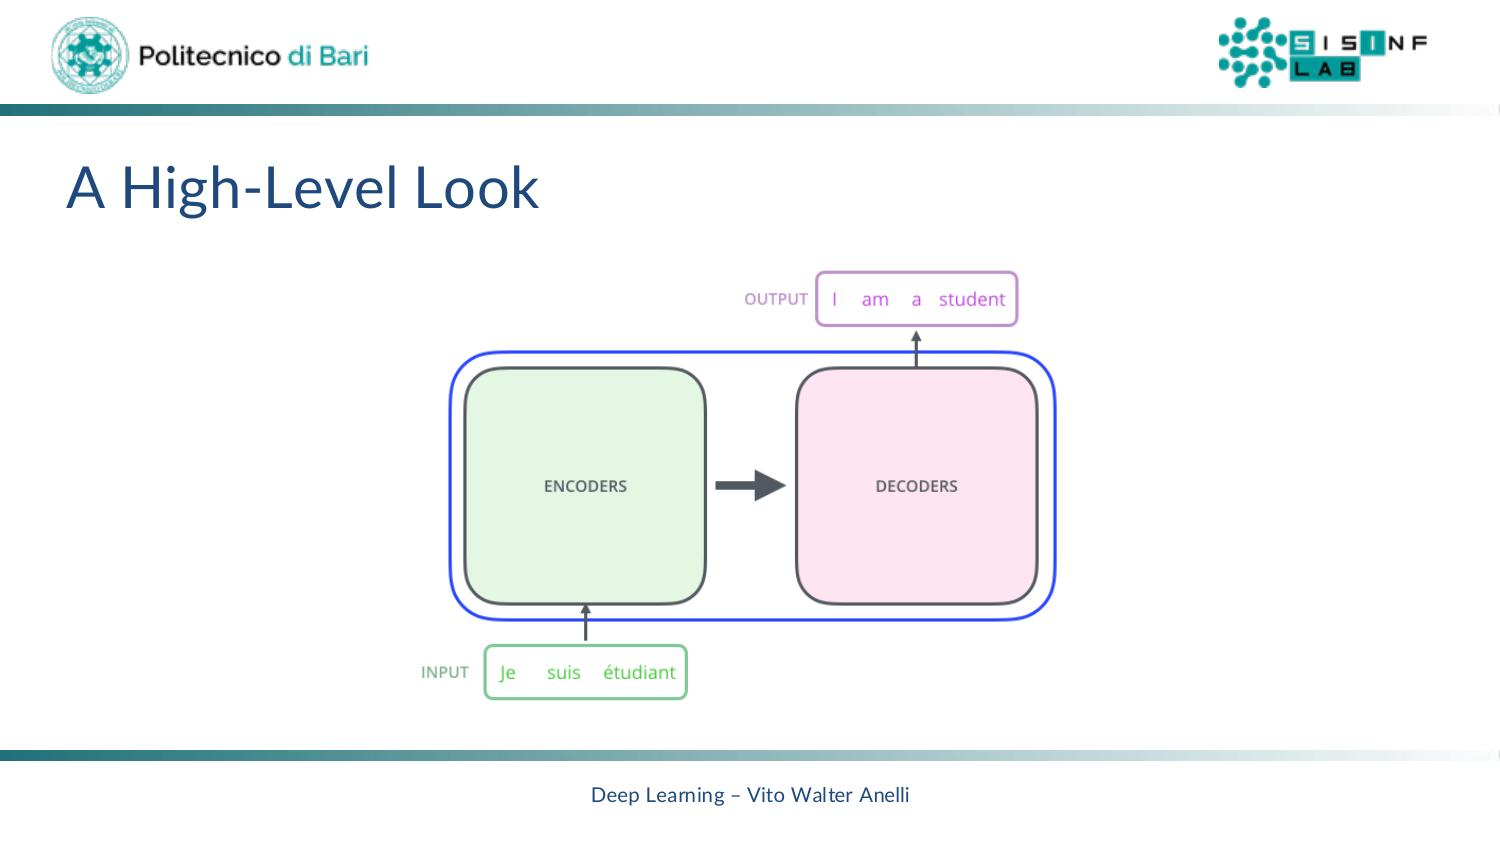
\includegraphics[width=0.62\linewidth]{figures/cf12_01_highlevel_enc_dec.jpg}
  \caption{Vista ad alto livello del Transformer. La frase di input
           (es.\ francese) attraversa lo stack di encoder; la
           rappresentazione prodotta alimenta lo stack di decoder che
           genera la traduzione (es.\ inglese) token per token.}
  \label{fig:highlevel_enc_dec}
\end{figure}

\subsection{Struttura Interna dell'Encoder}
\label{subsec:encoder-internal}

Ogni encoder e' composto da due sotto-livelli in cascata:

\begin{enumerate}
  \item \textbf{Self-Attention}: consente a ogni posizione di guardare
        tutte le altre posizioni durante la codifica, integrando il
        contesto globale nella rappresentazione di ciascun token.
        Le dipendenze tra percorsi esistono solo qui.
  \item \textbf{Feed-Forward Neural Network (FFN)}: applicata
        indipendentemente e identicamente a ciascuna posizione;
        non introduce dipendenze tra posizioni diverse, quindi i
        percorsi possono essere eseguiti in parallelo.
\end{enumerate}

\begin{figure}[H]
  \centering
  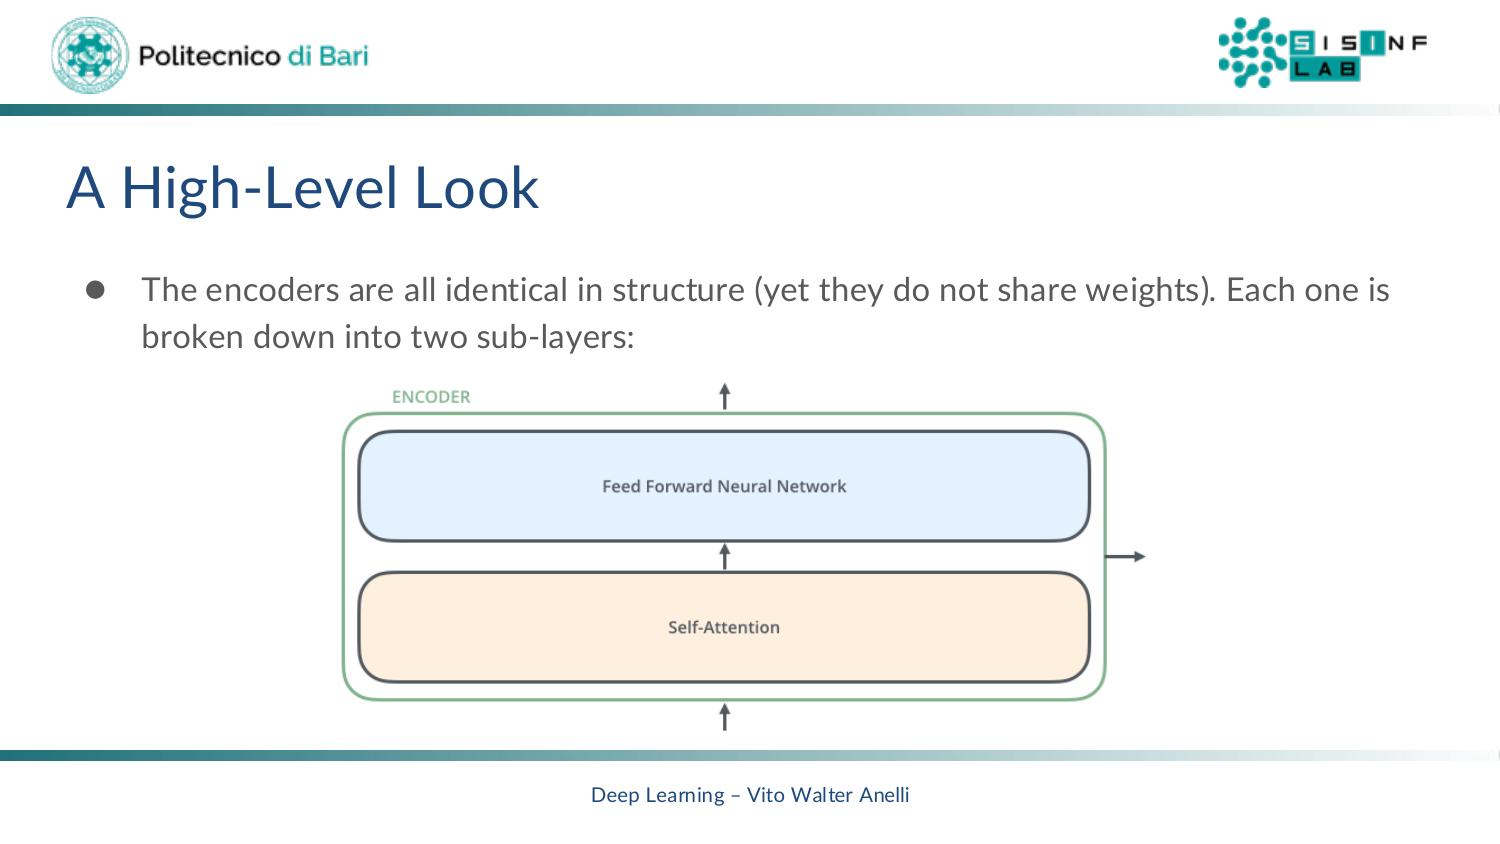
\includegraphics[width=0.60\linewidth]{figures/cf12_02_encoder_sublayers.jpg}
  \caption{Struttura interna di un singolo encoder: Self-Attention
           (rosa, sotto) produce rappresentazioni contestuali che vengono
           poi elaborate dal Feed-Forward Network (azzurro, sopra).}
  \label{fig:encoder_sublayers}
\end{figure}

\subsection{Struttura del Decoder}
\label{subsec:decoder-internal}

Il decoder aggiunge un terzo sotto-livello tra self-attention e FFN:
lo strato di \textbf{Encoder-Decoder Attention}, che consente al decoder
di focalizzarsi sulle parti rilevanti della sequenza di input. La
self-attention nel decoder e' \emph{mascherata}: ogni posizione puo'
attendere solo alle posizioni precedenti, preservando la causalita'.

\begin{figure}[H]
  \centering
  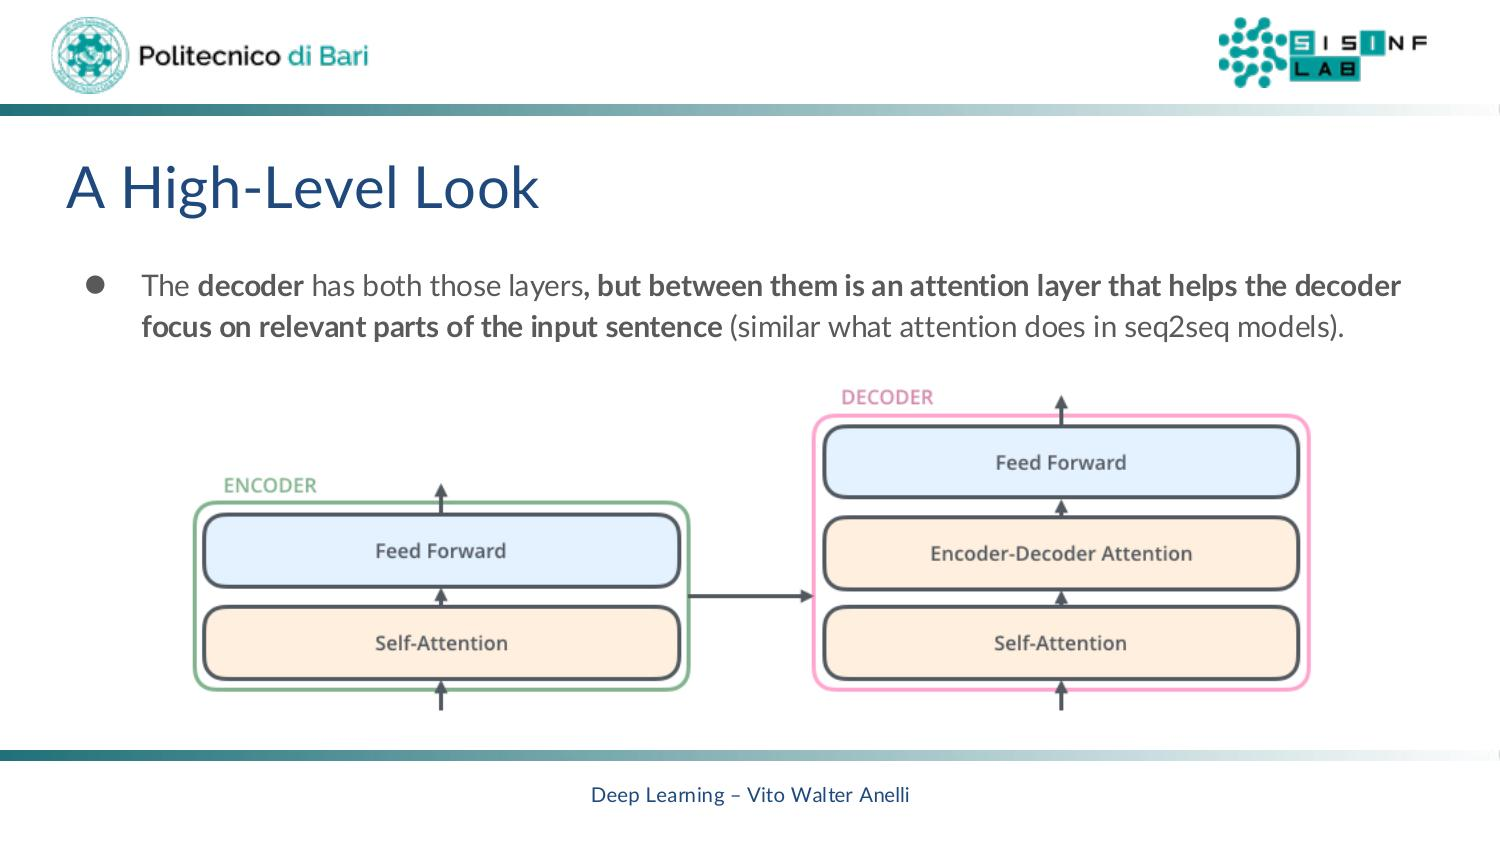
\includegraphics[width=0.82\linewidth]{figures/cf12_03_enc_dec_compare.jpg}
  \caption{Confronto tra encoder (sinistra, due sotto-livelli:
           Self-Attention + FFN) e decoder (destra, tre sotto-livelli:
           Masked Self-Attention, Encoder-Decoder Attention, FFN).
           L'Encoder-Decoder Attention riceve K e V dall'encoder.}
  \label{fig:enc_dec_compare}
\end{figure}

\subsection{Flusso dei Tensori}
\label{subsec:tensor-flow}

Prima di entrare nel primo encoder ogni token viene trasformato in un
vettore di dimensione $d_{\text{model}} = 512$ tramite una matrice
di embedding. Nei livelli successivi l'input e' l'output dell'encoder
precedente, sempre di dimensione $d_{\text{model}}$.

\begin{figure}[H]
  \centering
  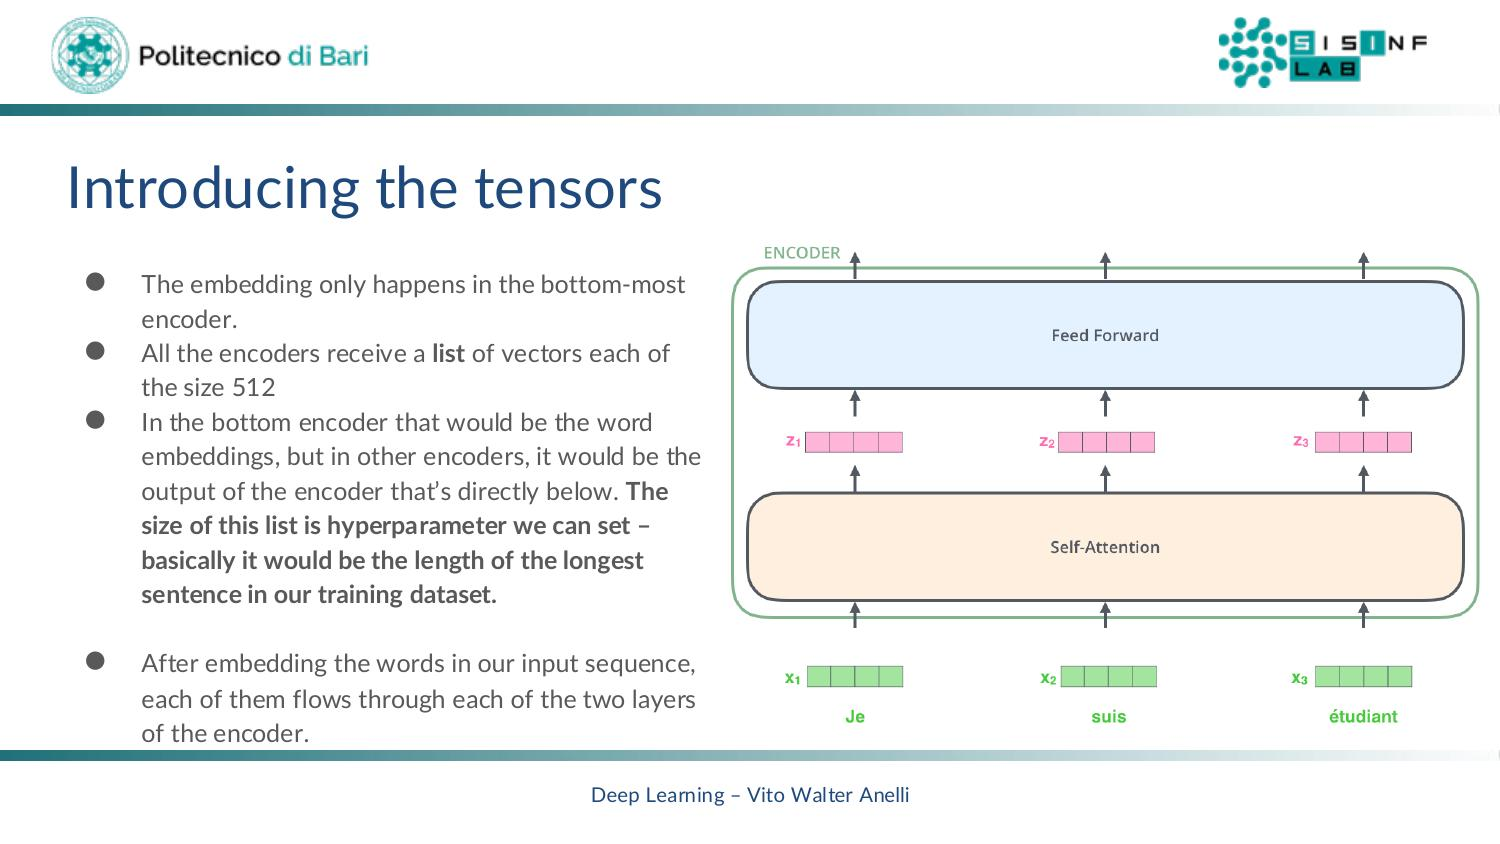
\includegraphics[width=0.78\linewidth]{figures/cf12_04_tensor_flow.jpg}
  \caption{Flusso dei tensori in un encoder. Ogni token $x_i$ (vettore
           di dimensione 512) scorre lungo il proprio percorso
           indipendente. La Self-Attention introduce dipendenze tra
           percorsi (vettori $z_i$ connessi); il FFN li processa in
           parallelo.}
  \label{fig:tensor_flow}
\end{figure}

%------------------------------------------------------------
\section{Self-Attention}
\label{sec:self-attention}

\subsection{Query, Key, Value}
\label{subsec:qkv}

Per ogni token $i$ si calcolano tre vettori tramite proiezione
lineare dell'embedding $\mathbf{x}_i$:

\begin{align}
  \mathbf{q}_i &= \mathbf{x}_i \, W^Q, \label{eq:query}\\
  \mathbf{k}_i &= \mathbf{x}_i \, W^K, \label{eq:key}\\
  \mathbf{v}_i &= \mathbf{x}_i \, W^V, \label{eq:value}
\end{align}

con $W^Q, W^K, W^V \in \mathbb{R}^{512 \times 64}$ apprese durante
il training. Il significato intuitivo e':

\begin{description}
  \item[Query $\mathbf{q}_i$] Rappresenta il token corrente nella
        ricerca: \emph{``Cosa sto cercando?''}
  \item[Key $\mathbf{k}_j$] Etichetta del token $j$:
        \emph{``Cosa offro come contenuto?''}
  \item[Value $\mathbf{v}_j$] Contenuto effettivo del token $j$:
        la rappresentazione che verra' aggregata.
\end{description}

Lo score di attenzione di $i$ verso $j$ e' il prodotto scalare
$s_{ij} = \mathbf{q}_i \cdot \mathbf{k}_j$, scalato per
$\sqrt{d_k}$ (con $d_k = 64$, fattore $= 8$) per stabilizzare
i gradienti, poi normalizzato con softmax:

\begin{equation}
  \alpha_{ij} = \frac{\exp(s_{ij}/\sqrt{d_k})}
                     {\sum_j \exp(s_{ij}/\sqrt{d_k})}.
  \label{eq:attn-weights}
\end{equation}

L'output per il token $i$ e' la somma pesata dei value:
$\mathbf{z}_i = \sum_j \alpha_{ij}\,\mathbf{v}_j$.

\subsection{Calcolo Matriciale}
\label{subsec:attn-matrix}

Impacchettando gli embedding in $X \in \mathbb{R}^{n \times 512}$
e calcolando $Q = XW^Q$, $K = XW^K$, $V = XW^V$, tutti i token
vengono elaborati simultaneamente:

\begin{equation}
  \boxed{
    Z = \mathrm{softmax}\!\left(\frac{Q K^\top}{\sqrt{d_k}}\right) V
  }
  \label{eq:self-attn-matrix}
\end{equation}

\begin{figure}[H]
  \centering
  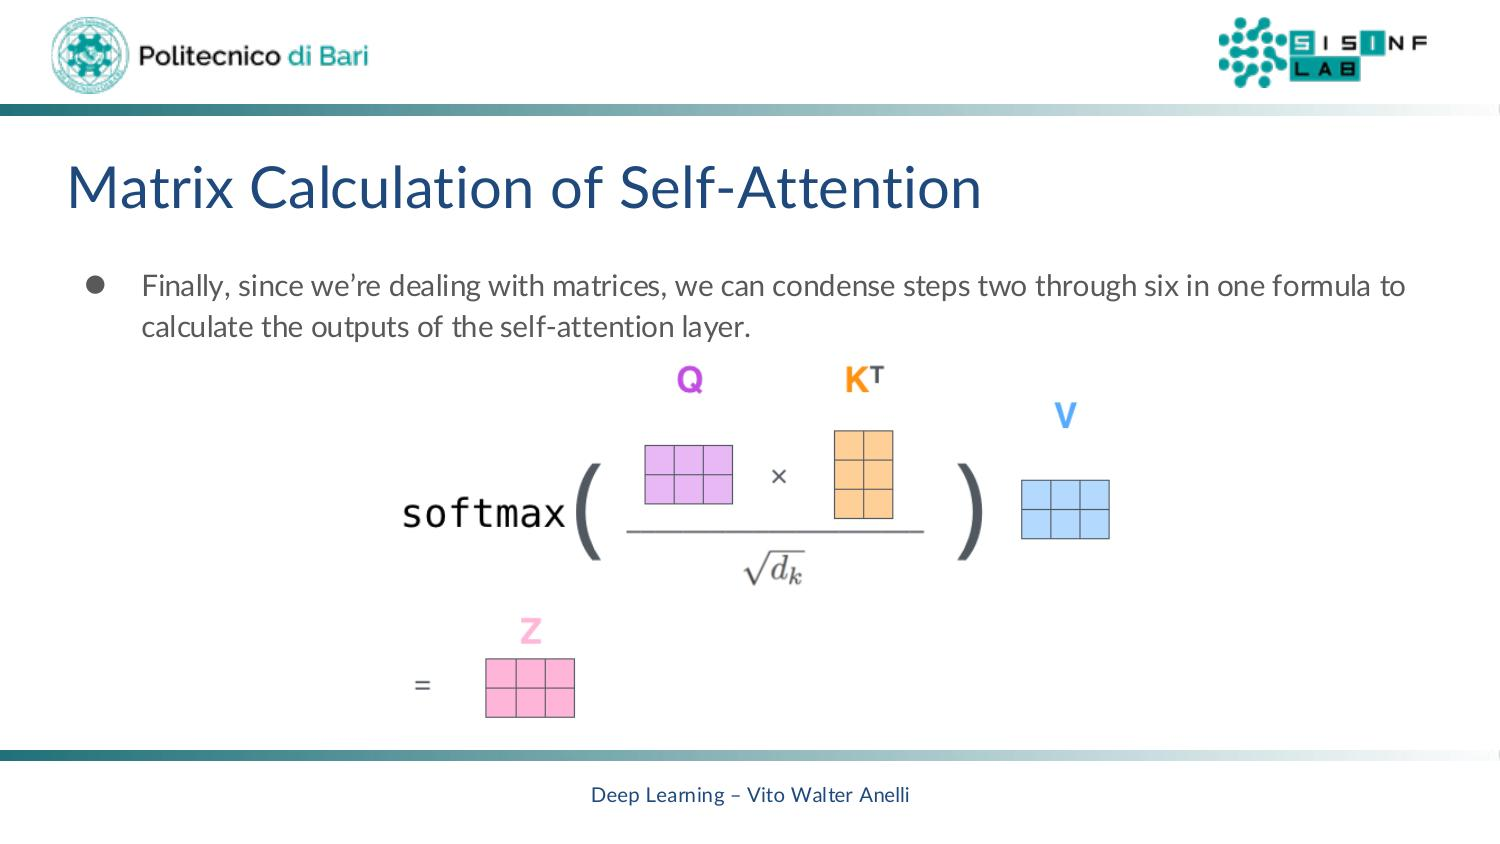
\includegraphics[width=0.62\linewidth]{figures/cf12_05_self_attn_formula.jpg}
  \caption{Formula matriciale della self-attention:
           $Z = \mathrm{softmax}(QK^\top/\sqrt{d_k})\,V$.
           $Q$ (viola) e $K^\top$ (arancione) sono $n \times 64$;
           $V$ (azzurro) e' $n \times 64$; $Z$ (rosa) e' $n \times 64$.}
  \label{fig:self_attn_formula}
\end{figure}

%------------------------------------------------------------
\section{Multi-Head Attention}
\label{sec:multihead}

L'attenzione \textbf{multi-head} (MHA) porta due vantaggi rispetto
alla singola testa:

\begin{enumerate}
  \item \textbf{Focus su posizioni diverse}: ogni testa si specializza
        su relazioni diverse (sintattiche, semantiche, posizionali).
  \item \textbf{Sottospazi multipli}: con $h$ teste si hanno $h$
        proiezioni indipendenti dello spazio semantico.
\end{enumerate}

Il paper originale usa $h = 8$ teste. Per ogni testa $i$ si
mantengono matrici separate $W_i^Q, W_i^K, W_i^V$ e si calcola
$Z_i$ con la formula~\eqref{eq:self-attn-matrix}. Poi:

\begin{equation}
  \mathrm{MHA}(Q,K,V) = \mathrm{Concat}(Z_0,\ldots,Z_7)\, W^O,
  \label{eq:mha}
\end{equation}

con $W^O \in \mathbb{R}^{h \cdot d_v \times d_{\text{model}}}$.

\begin{figure}[H]
  \centering
  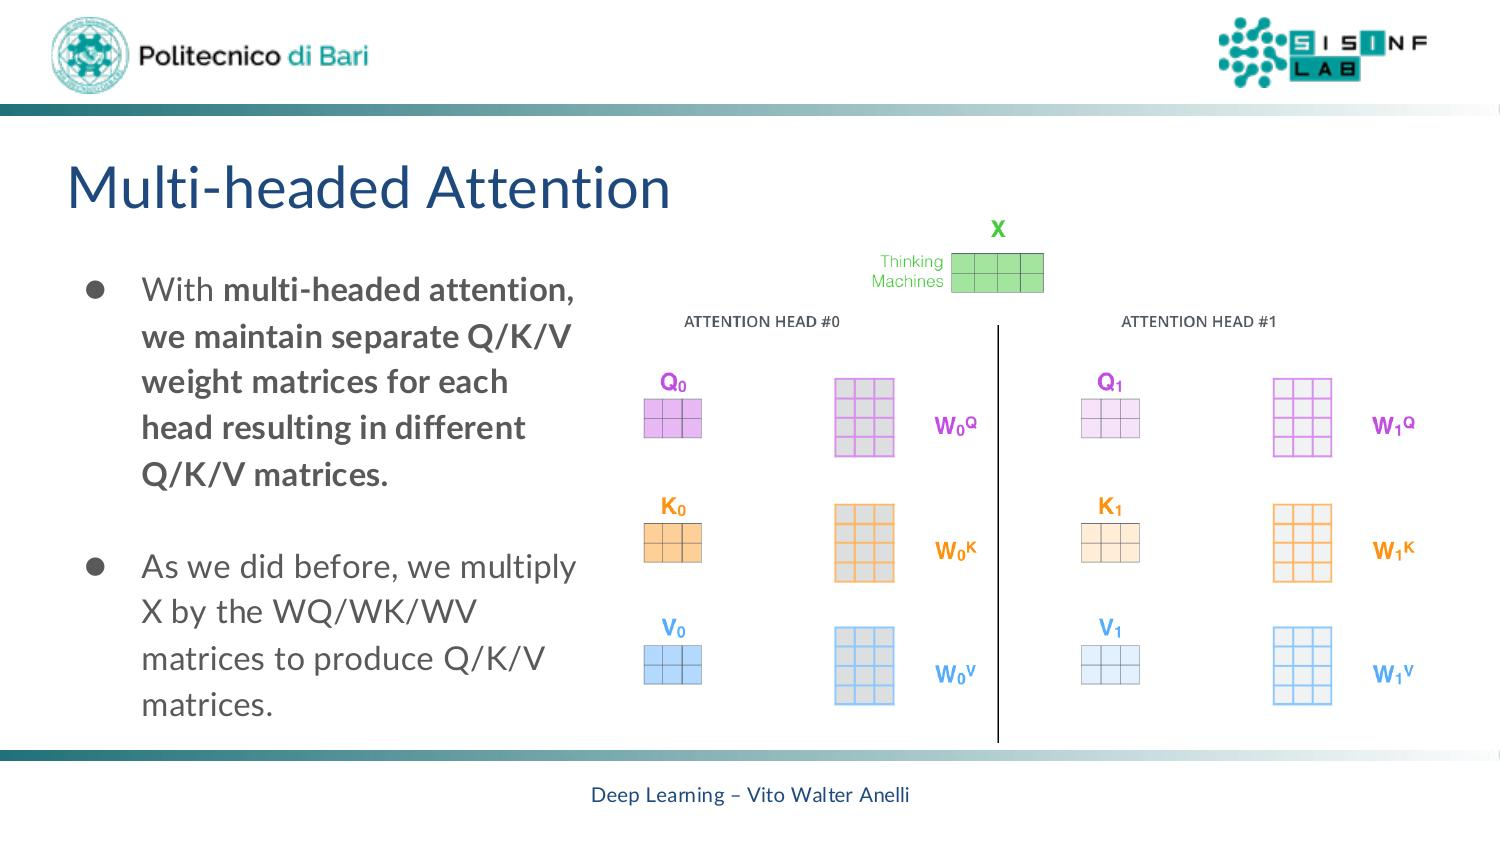
\includegraphics[width=0.82\linewidth]{figures/cf12_06_multihead_separate_qkv.jpg}
  \caption{Multi-head attention: set di pesi $W^Q$, $W^K$, $W^V$
           separati per ogni testa, producendo matrici Q, K, V
           distinte. Le due teste mostrate operano su diversi
           ``sottospazi di rappresentazione''.}
  \label{fig:multihead_qkv}
\end{figure}

\begin{figure}[H]
  \centering
  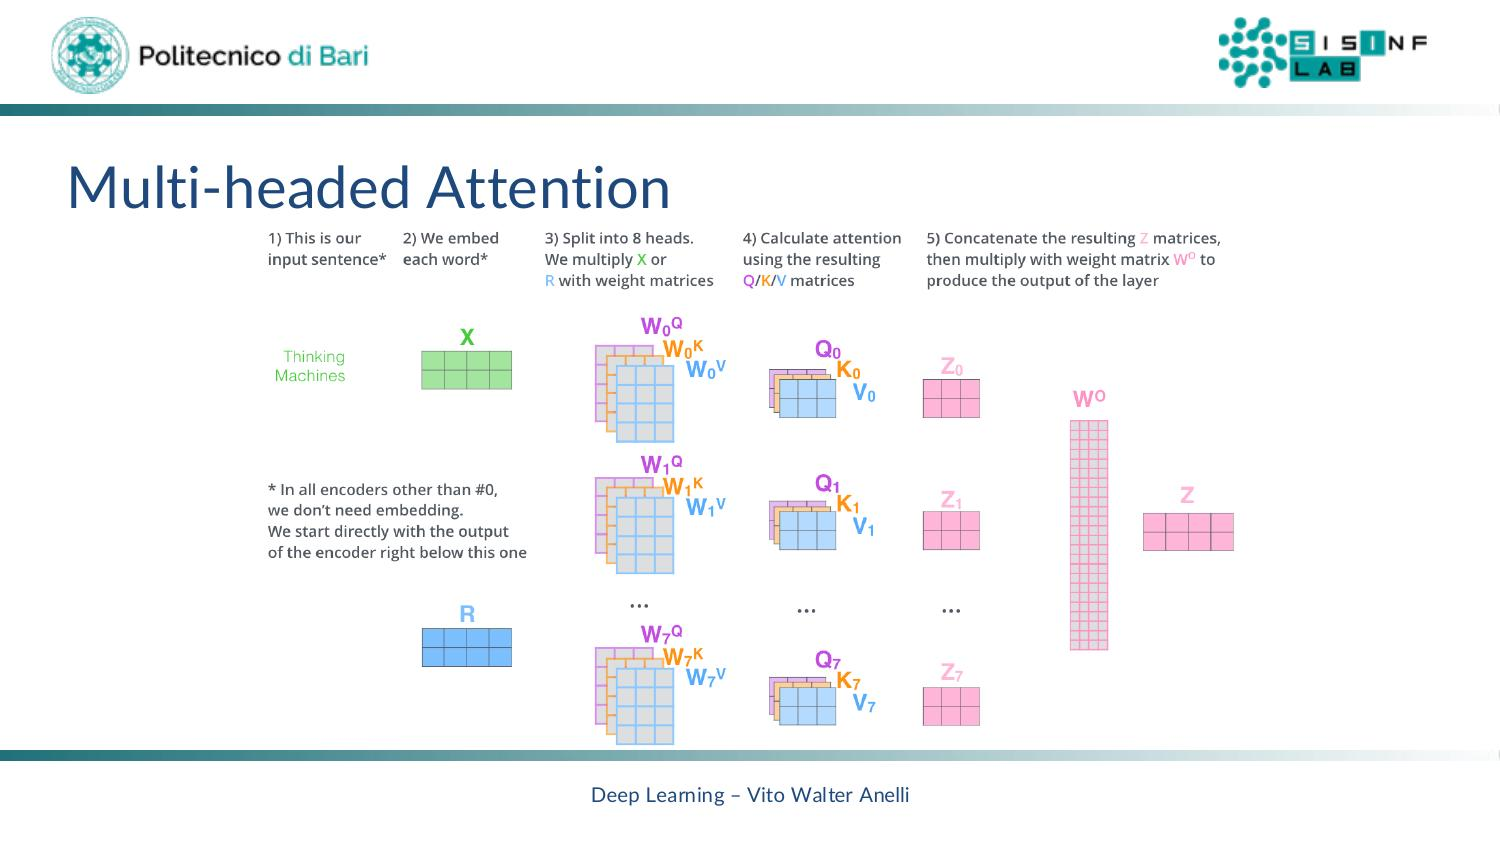
\includegraphics[width=0.95\linewidth]{figures/cf12_07_multihead_full_pipeline.jpg}
  \caption{Pipeline completa della Multi-Head Attention con $h=8$.
           (1) Frase di input. (2) Embedding. (3) Calcolo di
           $Q_i, K_i, V_i$ per ogni testa. (4) Calcolo di $Z_i$.
           (5) Concatenazione e proiezione con $W^O$.}
  \label{fig:multihead_pipeline}
\end{figure}

%------------------------------------------------------------
\section{Positional Encoding}
\label{sec:positional-encoding}

Il Transformer processa tutti i token in parallelo: senza segnale
di posizione, sarebbe invariante alla permutazione dei token.
Il \textbf{positional encoding} risolve il problema sommando un
vettore di posizione all'embedding:

\begin{figure}[H]
  \centering
  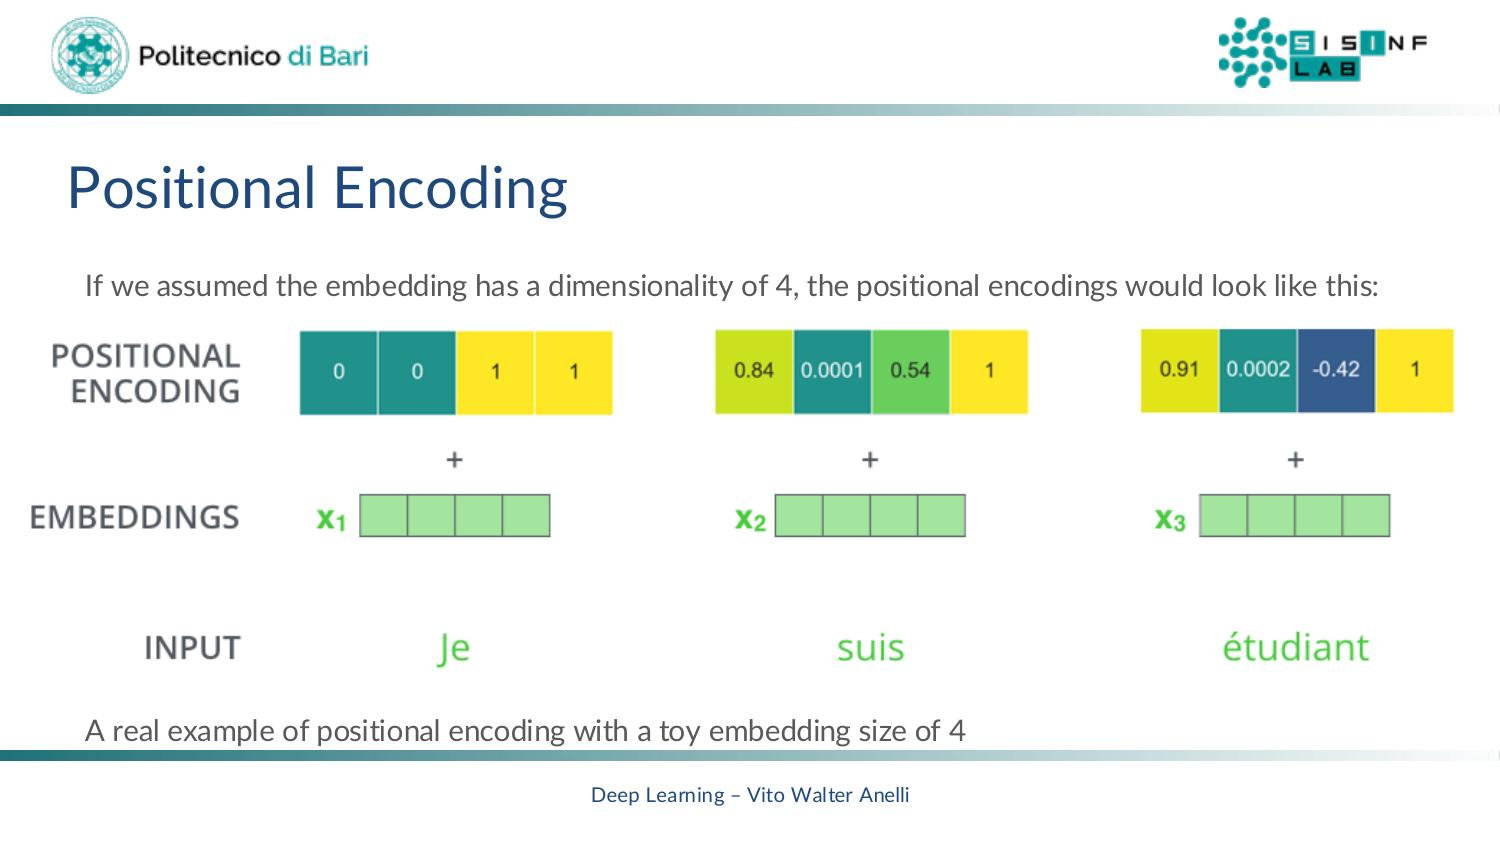
\includegraphics[width=0.88\linewidth]{figures/cf12_08_positional_encoding_example.jpg}
  \caption{Positional encoding con $d = 4$. Per ogni token si somma
           l'embedding $x_i$ al vettore PE corrispondente alla sua
           posizione. Posizioni diverse ricevono vettori diversi.}
  \label{fig:pe_example}
\end{figure}

La codifica sinusoidale deterministica del paper e':

\begin{align}
  \mathrm{PE}(pos,\, 2i)   &= \sin\!\left(\tfrac{pos}{10000^{2i/d_{\text{model}}}}\right),
  \label{eq:pe-sin}\\[4pt]
  \mathrm{PE}(pos,\, 2i+1) &= \cos\!\left(\tfrac{pos}{10000^{2i/d_{\text{model}}}}\right),
  \label{eq:pe-cos}
\end{align}

dove $pos$ e' la posizione e $i$ indicizza la dimensione. Le frequenze
variano geometricamente, permettendo di apprendere relazioni posizionali
relative a qualsiasi distanza. Non introduce parametri aggiuntivi e
generalizza a sequenze piu' lunghe di quelle di training.

\begin{figure}[H]
  \centering
  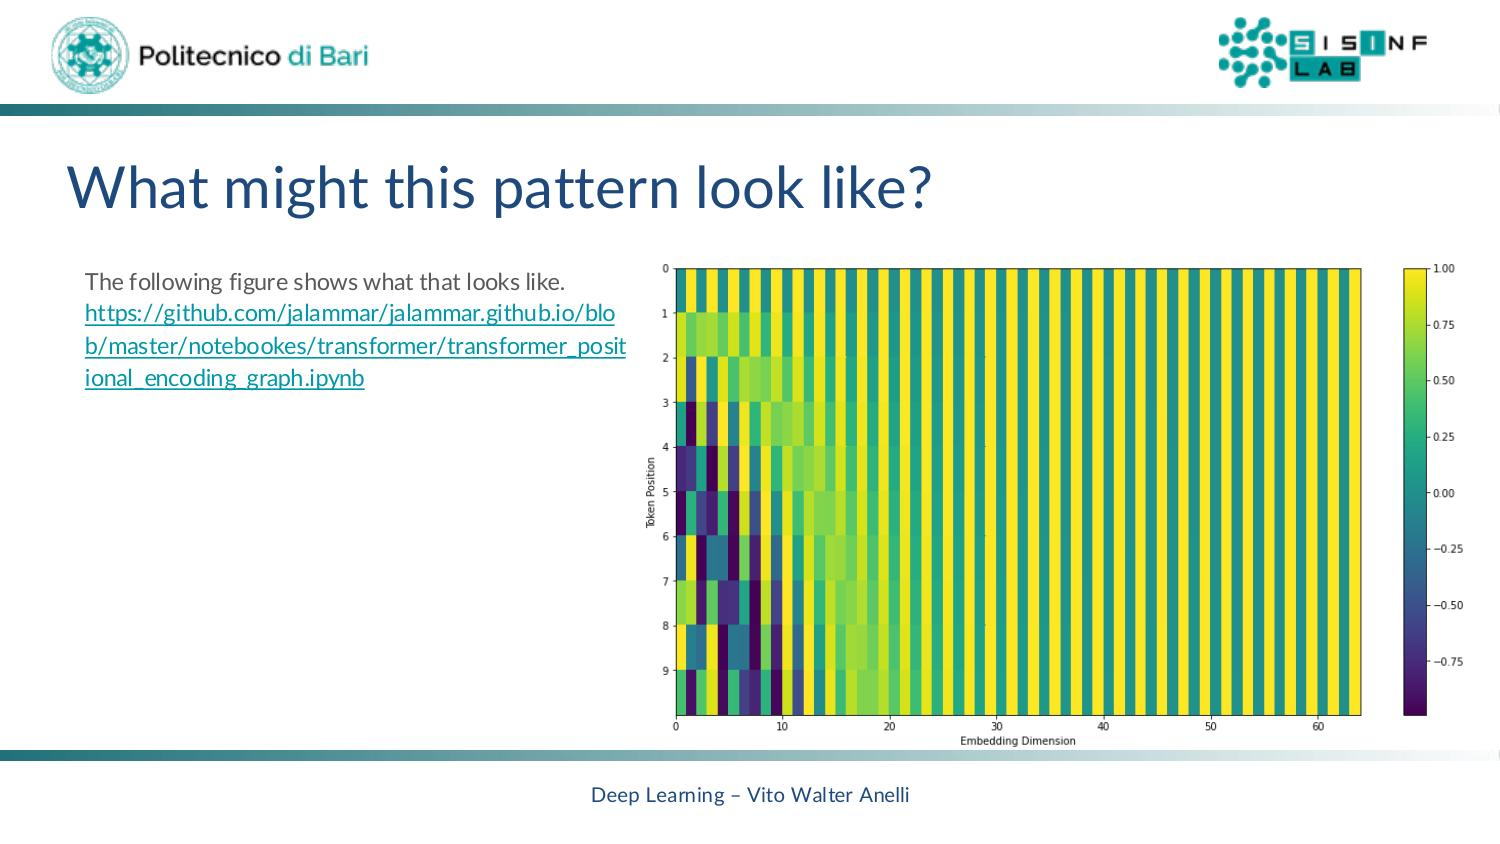
\includegraphics[width=0.72\linewidth]{figures/cf12_09_pe_heatmap.jpg}
  \caption{Heatmap dei vettori di PE ($y$: posizione del token,
           $x$: dimensione dell'embedding). Le prime dimensioni hanno
           alta frequenza (pattern fitto), le ultime bassa frequenza
           (pattern lento). Ogni riga e' il vettore PE per quella
           posizione.}
  \label{fig:pe_heatmap}
\end{figure}

%------------------------------------------------------------
\section{Residual Connections e Layer Normalization}
\label{sec:residuals}

Ogni sotto-livello e' avvolto da una \textbf{connessione residuale}
seguita da \textbf{layer normalization}:

\begin{equation}
  \mathbf{y} = \mathrm{LayerNorm}\!\left(\mathbf{x}
               + \mathrm{Sublayer}(\mathbf{x})\right).
  \label{eq:residual}
\end{equation}

Le connessioni residuali mitigano il vanishing gradient nelle reti
profonde. La layer normalization normalizza su ciascun esempio
(non sul batch), risultando piu' adatta alle sequenze di lunghezza
variabile rispetto alla batch normalization.

\begin{figure}[H]
  \centering
  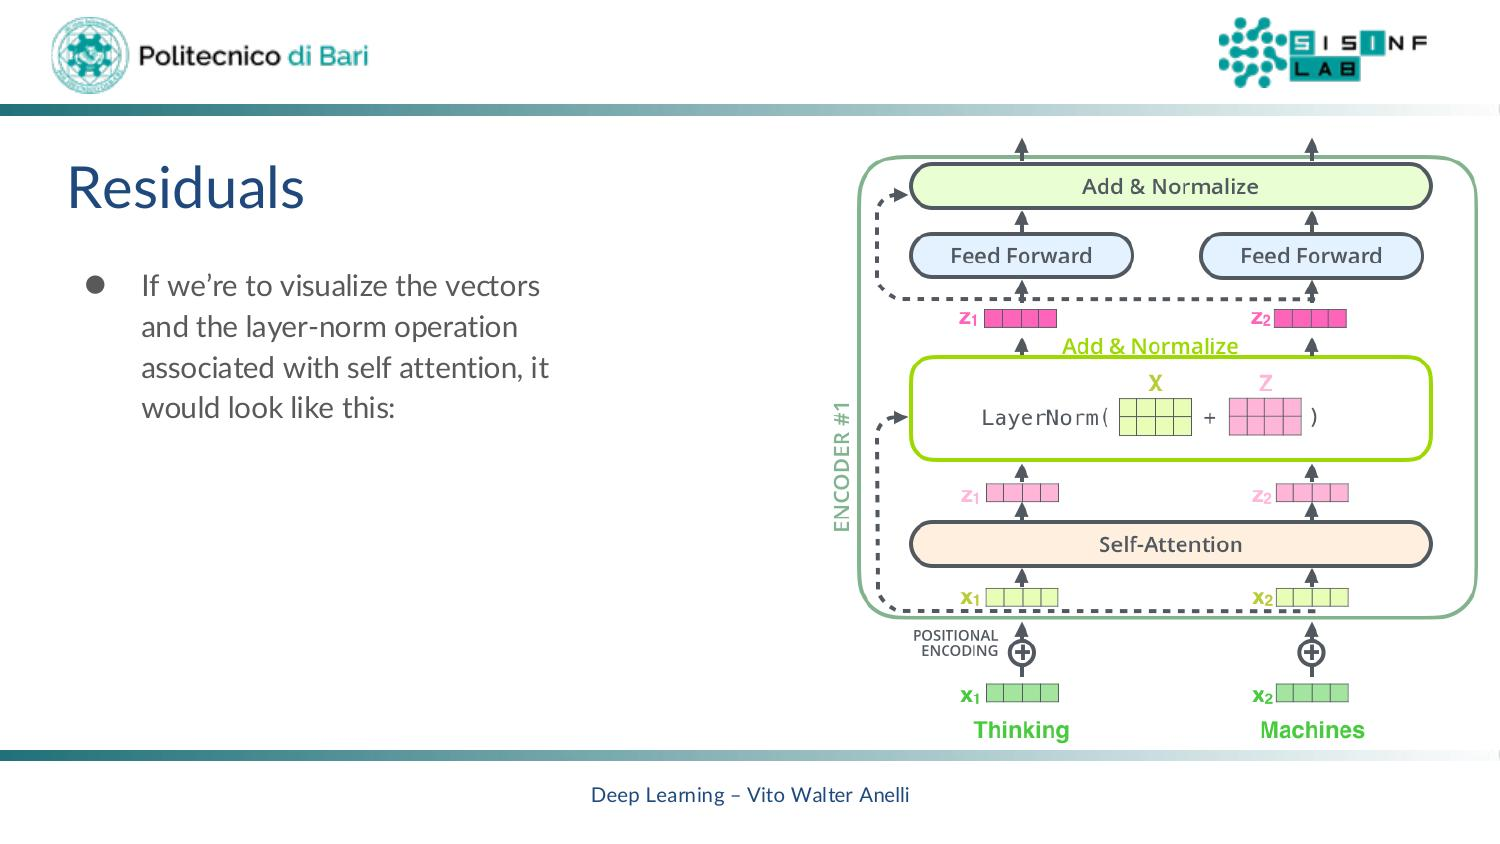
\includegraphics[width=0.62\linewidth]{figures/cf12_10_residuals_layernorm.jpg}
  \caption{Encoder con residual connections e layer normalization.
           I vettori $x_1, x_2$ (con PE sommato) attraversano
           Self-Attention producendo $z_1, z_2$; si applica
           $\mathrm{LayerNorm}(x + z)$; poi FFN con un secondo
           Add \& Normalize.}
  \label{fig:residuals_layernorm}
\end{figure}

%------------------------------------------------------------
\section{Lato Decoder}
\label{sec:decoder}

\subsection{Encoder-Decoder Attention e Generazione}
\label{subsec:dec-operation}

Il top encoder produce K e V che alimentano l'Encoder-Decoder
Attention di ogni decoder block; le Q provengono dal decoder stesso.
La generazione e' autoregressiva: al passo $t$ il decoder riceve
la sequenza generata fino a $t-1$ e produce la distribuzione su $w_t$.

\begin{figure}[H]
  \centering
  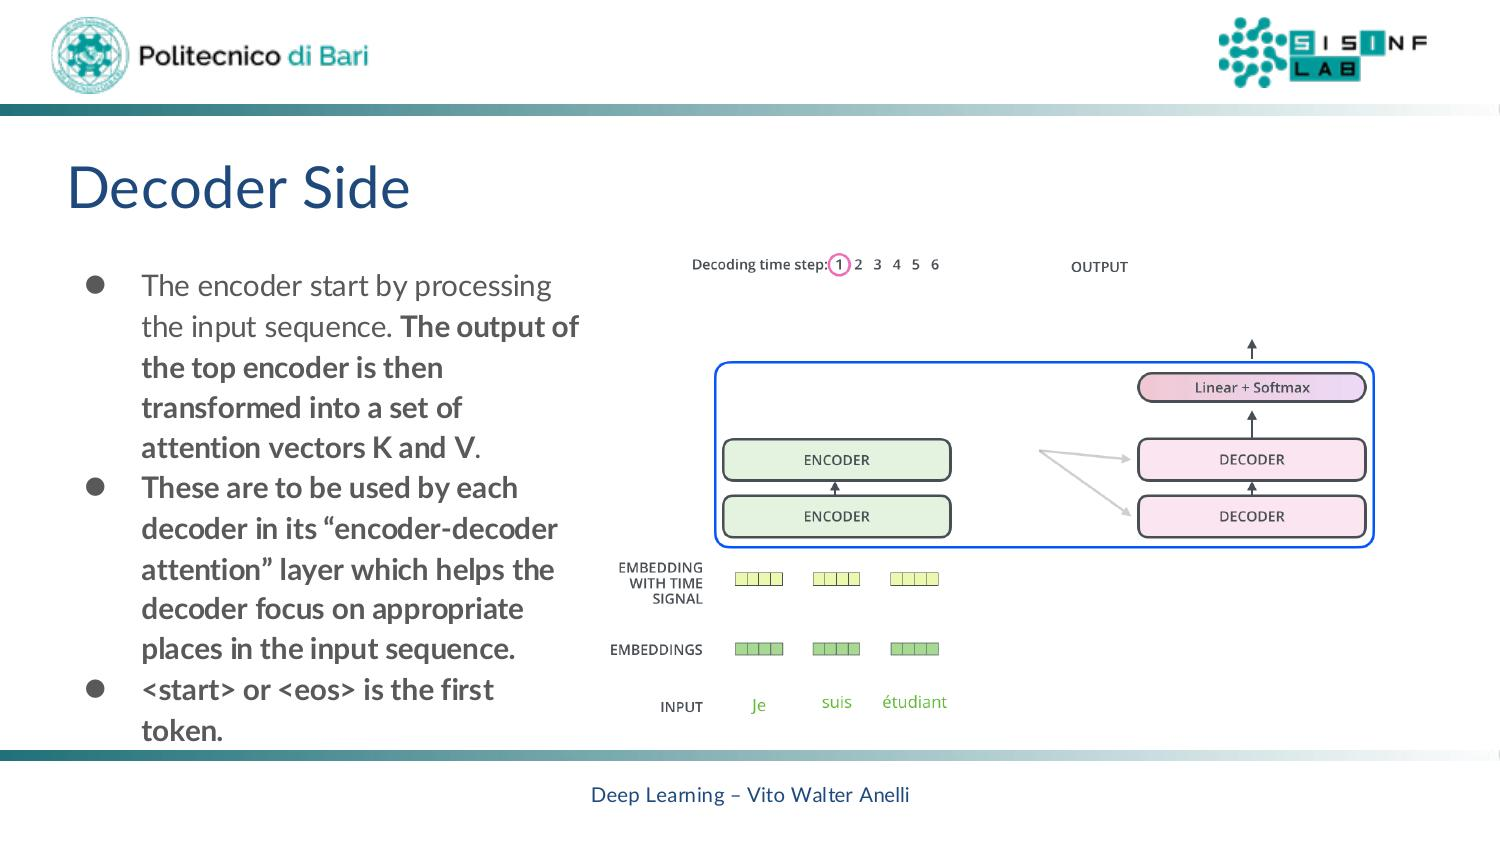
\includegraphics[width=0.82\linewidth]{figures/cf12_11_decoder_side.jpg}
  \caption{Lato decoder: K e V dell'encoder alimentano ogni decoder
           block. La generazione avviene passo per passo (time step
           1, 2, \ldots); ogni token prodotto viene rialimentato
           come input del passo successivo.}
  \label{fig:decoder_side}
\end{figure}

La masked self-attention garantisce la causalita' imponendo:

\begin{equation}
  \tilde{S}_{ij} = \begin{cases}
    S_{ij}  & j \le i,\\
    -\infty & j > i.
  \end{cases}
  \label{eq:attn-mask}
\end{equation}

\subsection{Strato Lineare e Softmax Finale}
\label{subsec:linear-softmax}

Il vettore di output del decoder ($d_{\text{model}}$ dim) viene
proiettato su $|\mathcal{V}|$ logit da uno strato lineare, poi
una softmax produce la distribuzione:

\begin{equation}
  P(w) = \frac{e^{\ell_w}}{\sum_{w'} e^{\ell_{w'}}}.
  \label{eq:output-softmax}
\end{equation}

\begin{figure}[H]
  \centering
  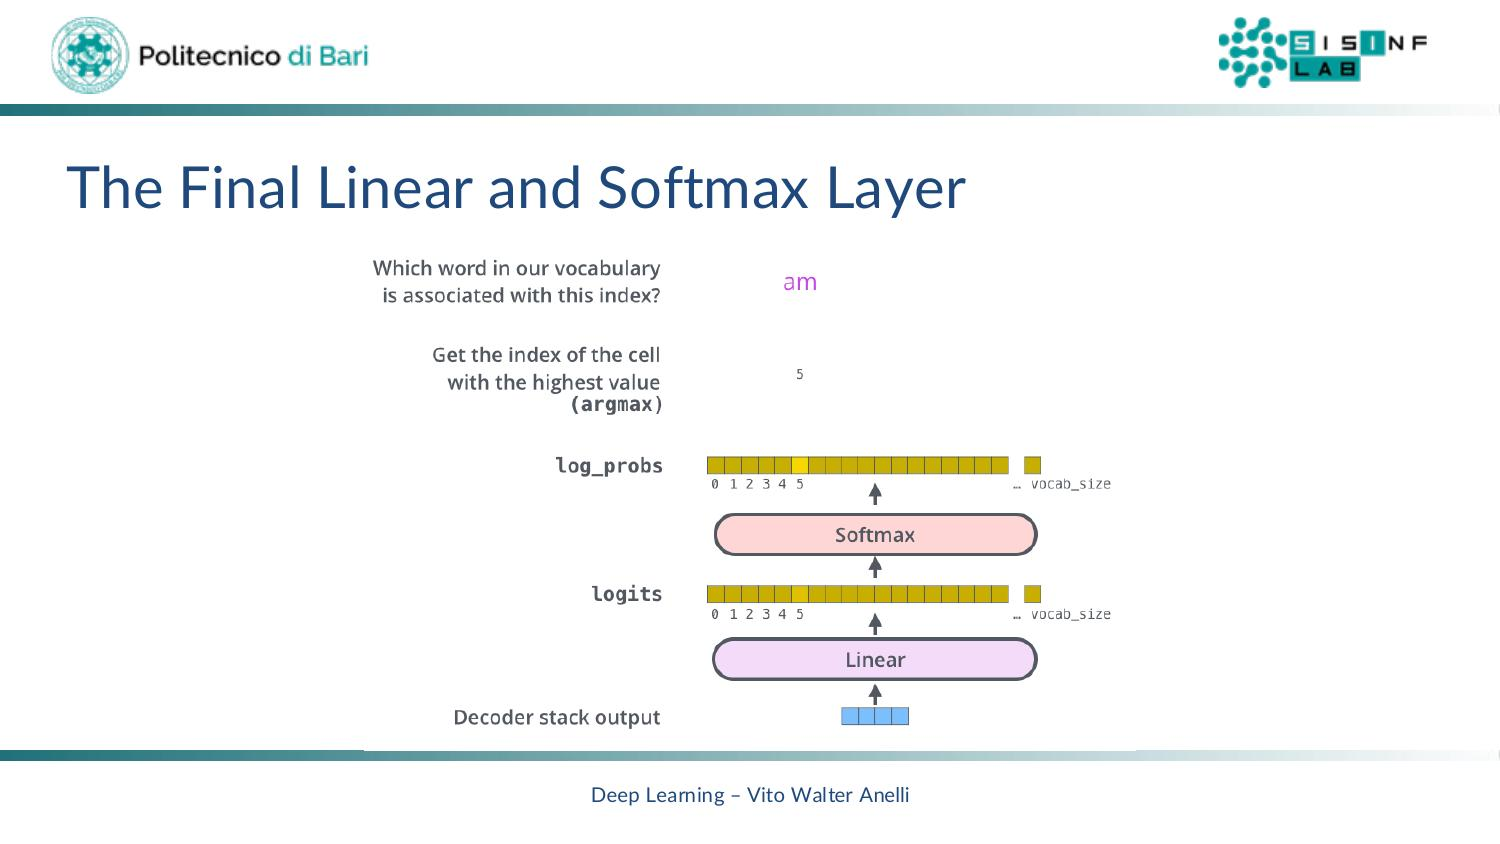
\includegraphics[width=0.56\linewidth]{figures/cf12_12_linear_softmax.jpg}
  \caption{Pipeline di output: il decoder stack output passa attraverso
           lo strato lineare (logits, dim $= |\mathcal{V}|$), poi la
           softmax produce le log-probabilita'. L'argmax sull'indice
           restituisce il token predetto (es.\ ``am'' all'indice 5).}
  \label{fig:linear_softmax}
\end{figure}

%------------------------------------------------------------
\section{Addestramento del Transformer}
\label{sec:training}

Durante il training si usa il \emph{teacher forcing}: il decoder
riceve l'intera sequenza target shiftata di una posizione a destra
(\texttt{<start>}, $w_1^*, w_2^*, \ldots$). La masked self-attention
garantisce che la posizione $t$ non veda i token successivi.

La loss e' la cross-entropy media su tutte le posizioni:

\begin{equation}
  \mathcal{L} = -\frac{1}{T}\sum_{t=1}^{T}
                \log P\!\left(w_t^* \mid w_1^*, \ldots, w_{t-1}^*\right).
  \label{eq:loss}
\end{equation}

%------------------------------------------------------------
\section{BERT}
\label{sec:bert}

\subsection{Architettura}
\label{subsec:bert-arch}

BERT (\emph{Bidirectional Encoder Representations from Transformers})
usa solo lo stack di encoder senza decoder. Essendo non causale,
ogni token puo' attendere a tutti gli altri in entrambe le direzioni
(\emph{bidirezionale}). Le due varianti principali sono:

\begin{itemize}
  \item \textbf{BERT Base}: 12 layer, $d_{\text{model}} = 768$,
        12 teste, 110M parametri.
  \item \textbf{BERT Large}: 24 layer, $d_{\text{model}} = 1024$,
        16 teste, 340M parametri.
\end{itemize}

Il primo token e' sempre \texttt{[CLS]} (\emph{classification}): il
suo vettore di output aggrega informazione globale sulla sequenza ed
e' usato per i task di classificazione.

\begin{figure}[H]
  \centering
  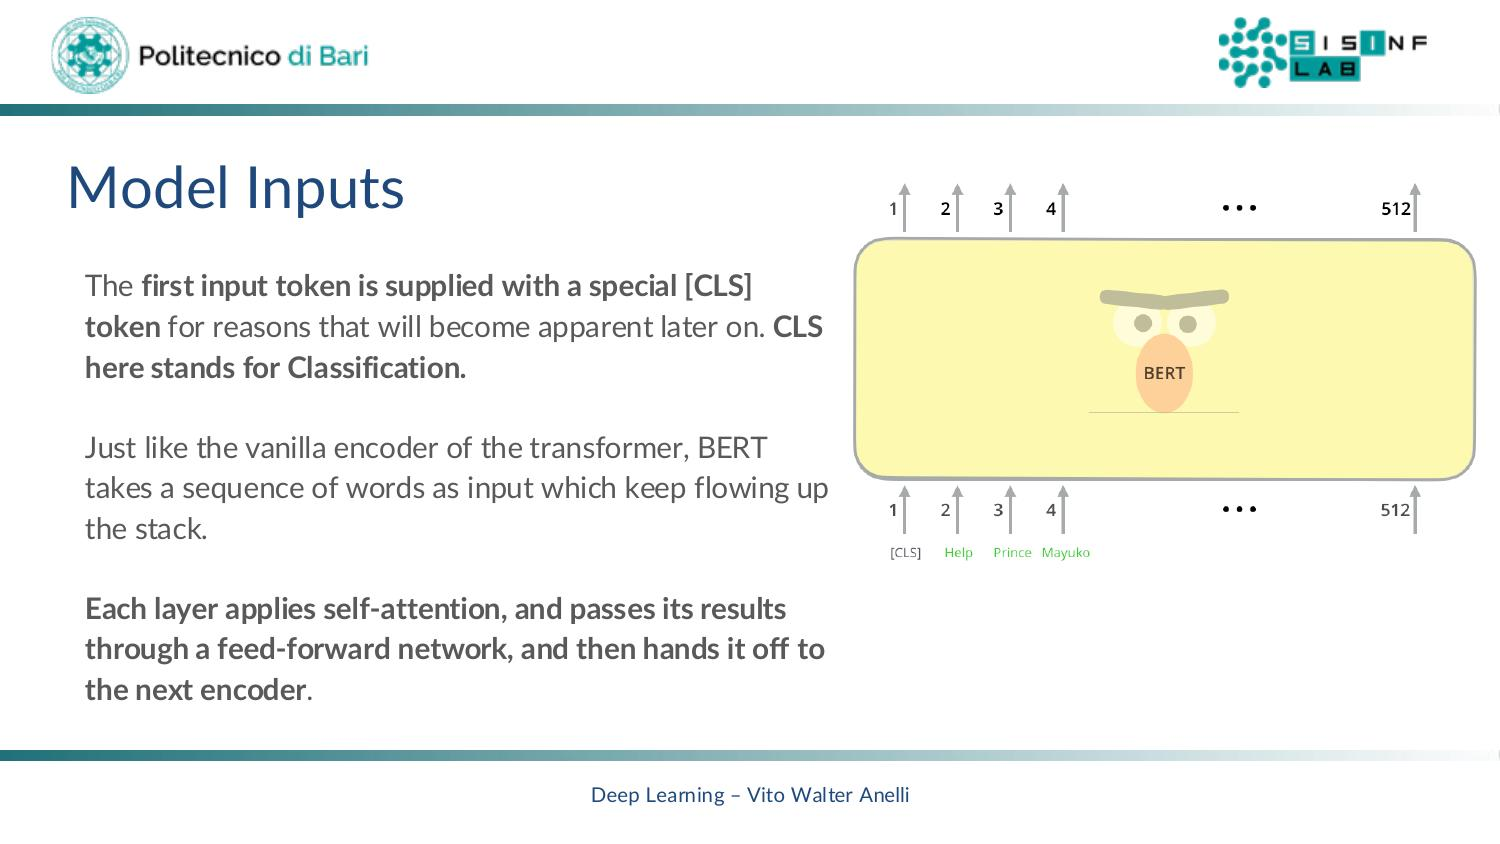
\includegraphics[width=0.70\linewidth]{figures/cf12_13_bert_inputs.jpg}
  \caption{Input di BERT: la sequenza inizia con \texttt{[CLS]},
           seguita dai token della frase. I 12 encoder layer
           producono un vettore di output per ogni posizione.}
  \label{fig:bert_inputs}
\end{figure}

\begin{figure}[H]
  \centering
  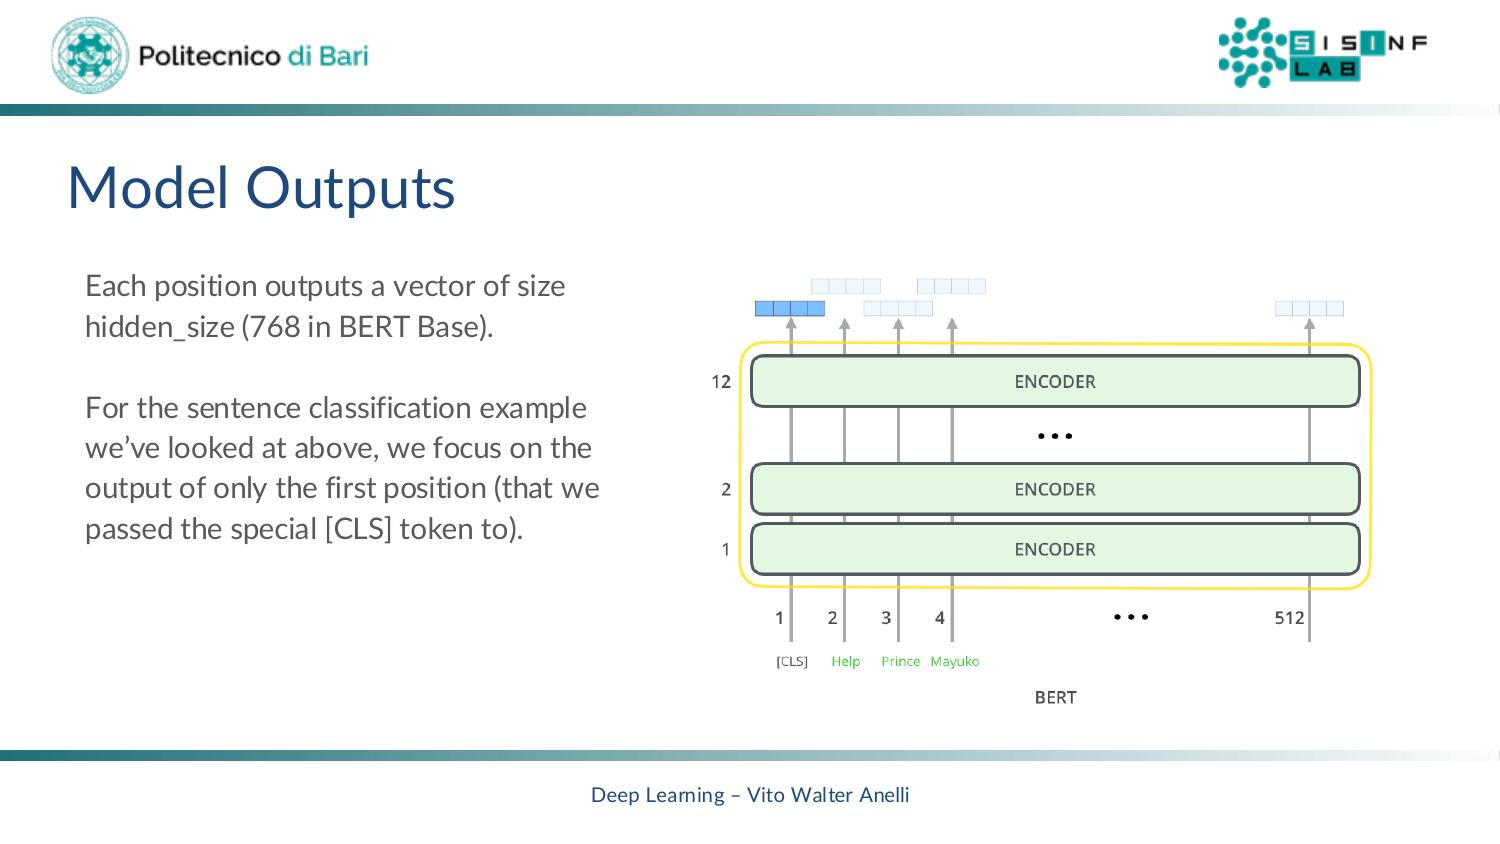
\includegraphics[width=0.70\linewidth]{figures/cf12_14_bert_outputs.jpg}
  \caption{Output di BERT per la classificazione. Ogni posizione
           produce un vettore di 768 dim. Per task a livello di frase
           si usa solo il vettore \texttt{[CLS]} (posizione 1),
           passato a un classificatore lineare + softmax.}
  \label{fig:bert_outputs}
\end{figure}

\subsection{Pre-training}
\label{subsec:bert-pretrain}

\begin{description}
  \item[Masked Language Model (MLM)] Il 15\% dei token viene
        selezionato: l'80\% sostituito con \texttt{[MASK]}, il 10\%
        con token casuale, il 10\% lasciato invariato. Il modello
        deve predire il token originale.
  \item[Next Sentence Prediction (NSP)] Il modello decide se la
        frase B segue naturalmente la frase A nel testo originale.
\end{description}

\subsection{Utilizzo}
\label{subsec:bert-use}

\begin{description}
  \item[Fine-tuning] Si aggiunge un classificatore sul vettore
        \texttt{[CLS]} e si ri-addestra l'intero modello con
        learning rate ridotto.
  \item[Feature extraction] BERT e' congelato; i vettori contestuali
        sono usati come features per un modello esterno. La
        combinazione degli ultimi 4 layer raggiunge risultati
        vicini al fine-tuning su task come NER.
\end{description}

%------------------------------------------------------------
\section{GPT}
\label{sec:gpt}

\subsection{Architettura Decoder-Only}
\label{subsec:gpt-arch}

GPT (\emph{Generative Pretrained Transformer}) usa solo lo stack di
decoder (\emph{decoder-only}): l'Encoder-Decoder Attention viene
rimosso; ogni blocco ha solo Masked Self-Attention + FFN. Il modello
e' autoregressivo: genera un token alla volta condizionandosi su
tutti quelli precedenti.

\subsection{Masked Self-Attention: Dettaglio Numerico}
\label{subsec:masked-sa}

\begin{figure}[H]
  \centering
  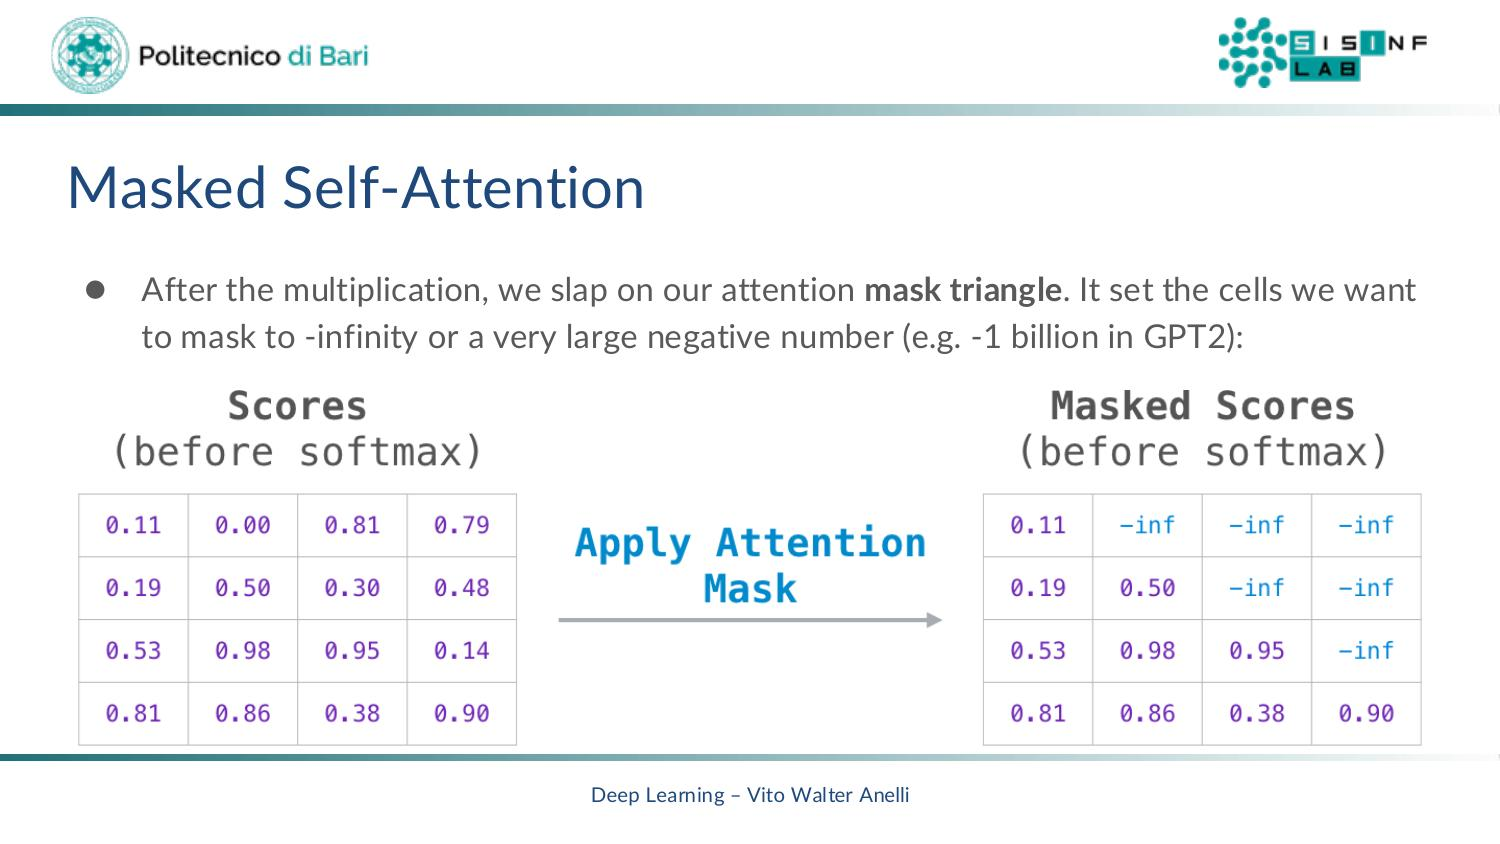
\includegraphics[width=0.88\linewidth]{figures/cf12_16_masked_attn_triangle.jpg}
  \caption{Applicazione della maschera triangolare. Sinistra: score
           originali. Destra: score mascherati con $-\infty$ nelle
           posizioni future (triangolo superiore). La riga $i$ puo'
           attendere solo alle colonne $j \le i$.}
  \label{fig:masked_triangle}
\end{figure}

\begin{figure}[H]
  \centering
  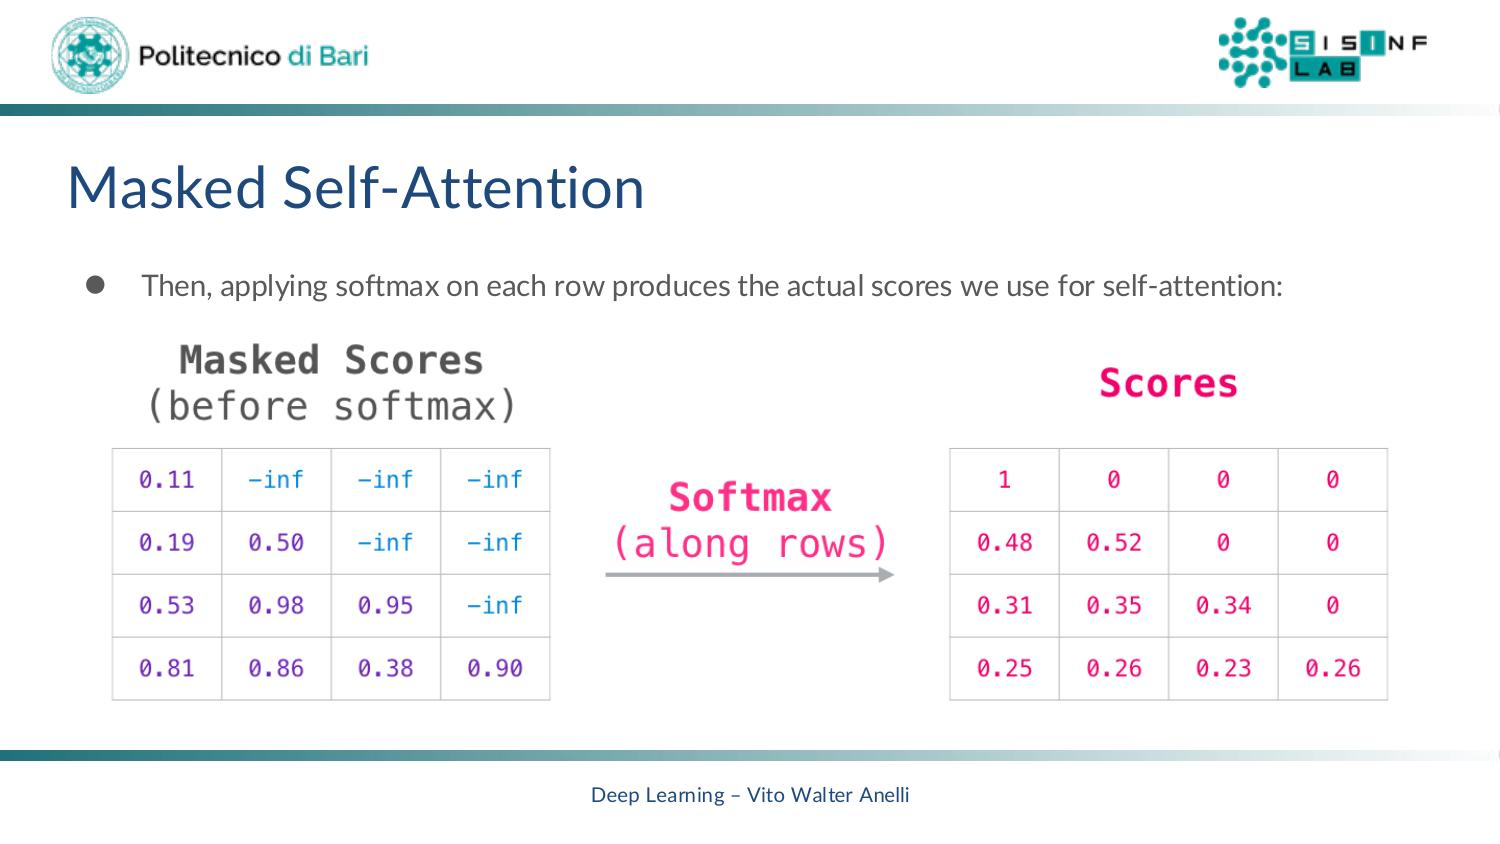
\includegraphics[width=0.88\linewidth]{figures/cf12_17_masked_attn_softmax.jpg}
  \caption{Dopo la softmax per righe, i valori $-\infty$ diventano 0.
           La prima riga attende solo se stessa $(1, 0, 0, 0)$;
           la quarta puo' attendere a tutti e 4 i token.}
  \label{fig:masked_softmax}
\end{figure}

\subsection{Decoder Block e Generazione}
\label{subsec:gpt-gen}

\begin{figure}[H]
  \centering
  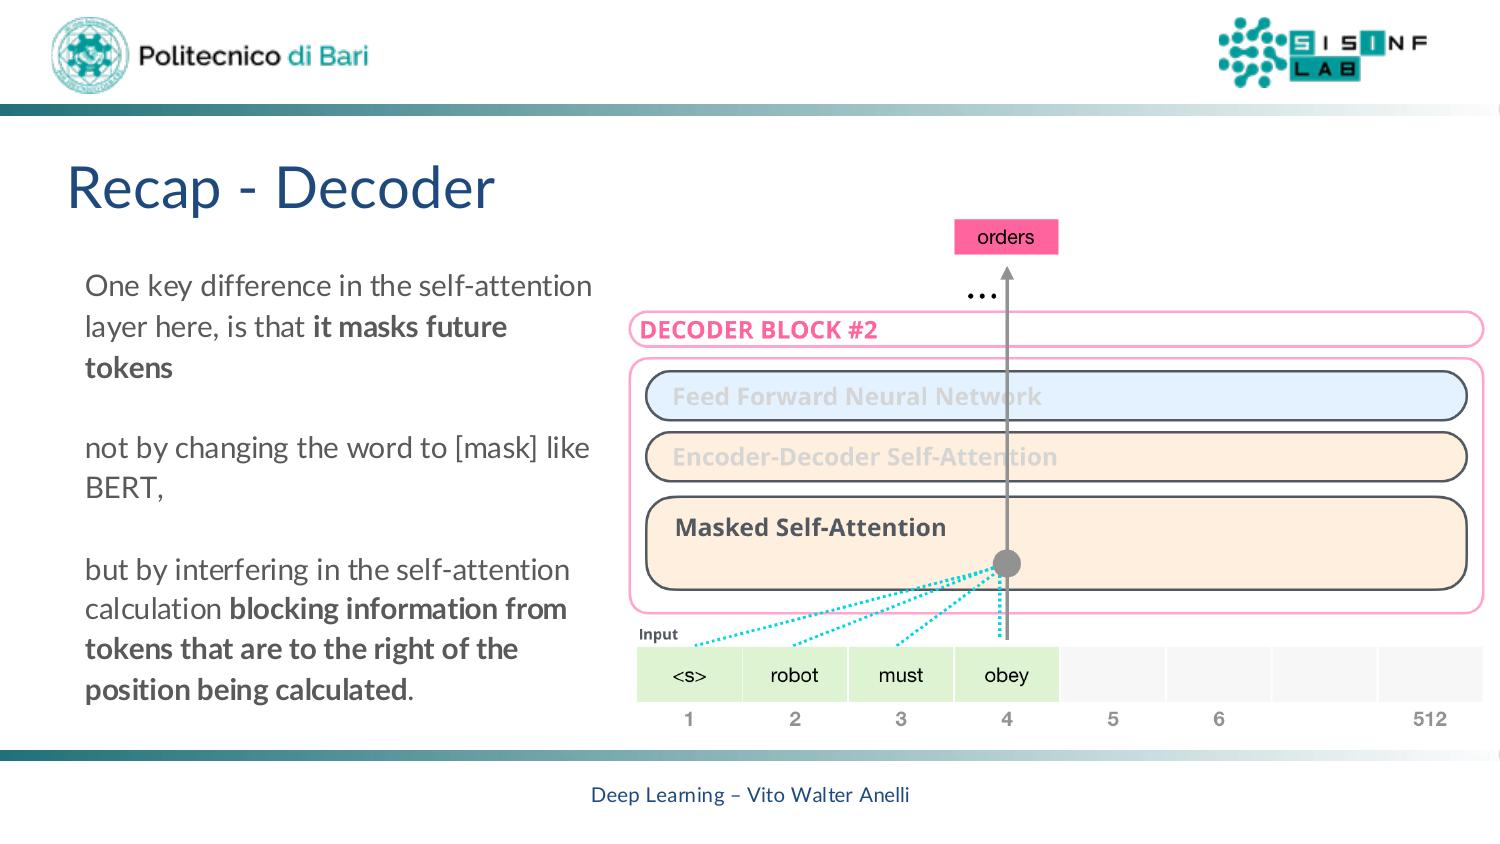
\includegraphics[width=0.82\linewidth]{figures/cf12_15_decoder_masked_recap.jpg}
  \caption{Decoder block di GPT: il Masked Self-Attention blocca le
           informazioni dai token alla destra della posizione corrente
           interferendo nel calcolo degli score, non sostituendo i
           token con \texttt{[MASK]} come BERT.}
  \label{fig:decoder_masked}
\end{figure}

Durante l'inferenza GPT genera un token alla volta (\emph{auto-regressione}).
La \textbf{KV cache} conserva le chiavi e i valori dei token gia'
elaborati, evitando il ricalcolo completo ad ogni passo.
Il parametro \textbf{top-k} controlla la varieta': con $k=1$ si usa
il token piu' probabile (greedy); con $k > 1$ si campiona tra i $k$
piu' probabili.

\subsection{Pipeline Self-Attention in GPT-2 Small}
\label{subsec:gpt2-pipeline}

GPT-2 Small: $h = 12$ teste, $d_{\text{model}} = 768$, $d_k = 64$.

\begin{description}
  \item[Fase 1 -- q, k, v] Il vettore di input (768) e' moltiplicato
        per una matrice $768 \times 2304$, ottenendo per
        concatenazione i vettori q, k, v (768 dim ciascuno).
  \item[Fase 1.5 -- Split] q (e analogamente k, v) viene rimodellato
        in $12 \times 64$: una riga per testa.
\end{description}

\begin{figure}[H]
  \centering
  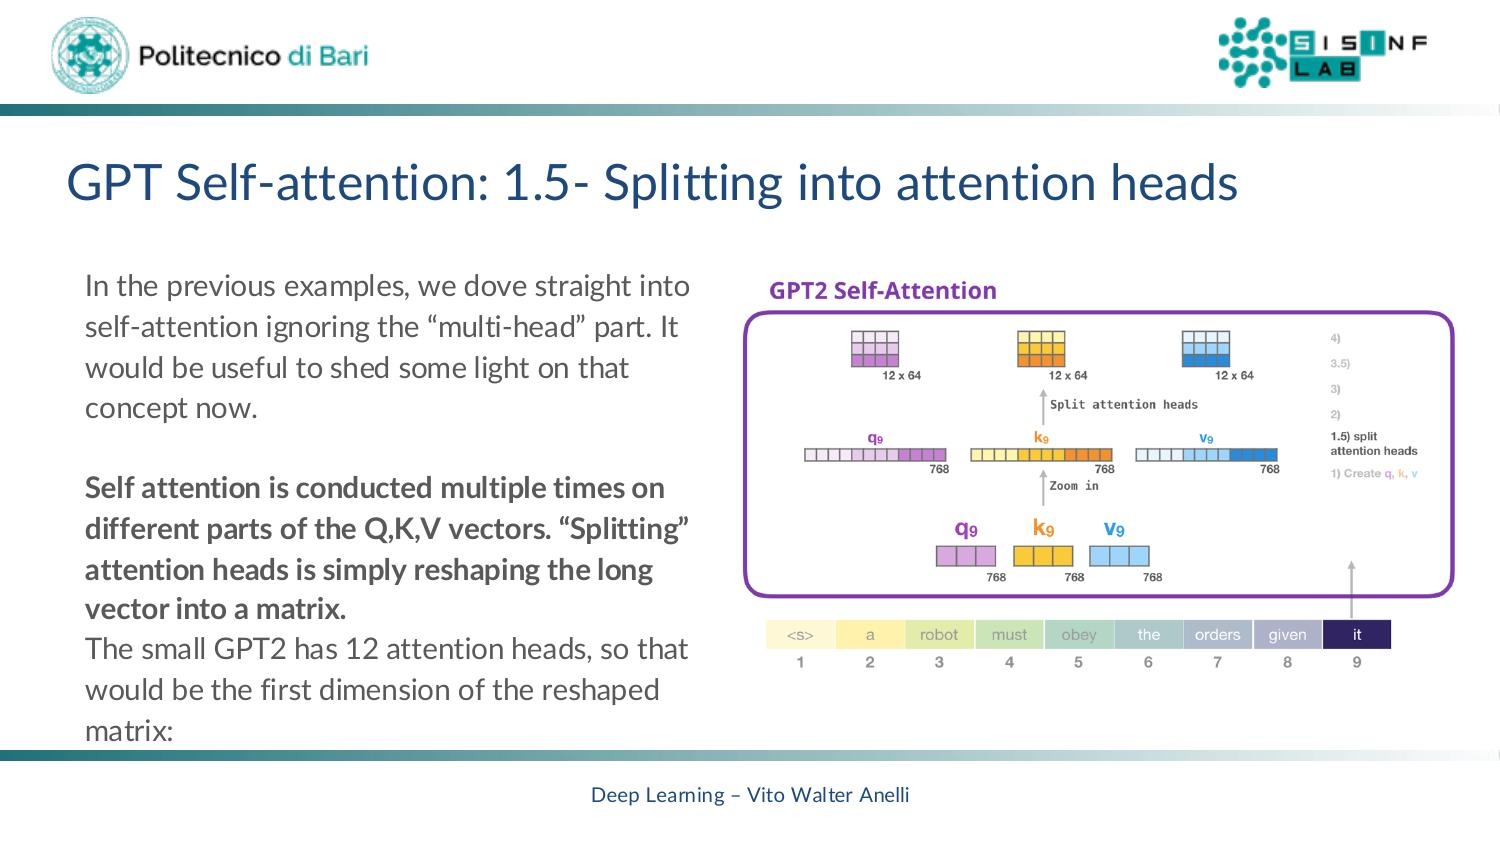
\includegraphics[width=0.85\linewidth]{figures/cf12_18_gpt_head_split.jpg}
  \caption{Split delle teste in GPT-2. I vettori q, k, v di 768 dim
           sono rimodellati in matrici $12 \times 64$. Ogni testa opera
           su 64 dimensioni della rappresentazione originale.}
  \label{fig:head_split}
\end{figure}

\begin{description}
  \item[Fase 2 -- Scoring] Ogni testa calcola il prodotto scalare
        tra la propria query e le chiavi di tutti i token precedenti
        (KV cache), scalato per $\sqrt{64}$.
  \item[Fase 3 -- Somma] I value sono pesati dagli score softmaxati
        e sommati.
  \item[Fase 3.5 -- Merge] I 12 vettori di output sono concatenati
        (768 dim totali).
  \item[Fase 4 -- Proiezione] Il vettore concatenato e' proiettato
        da $W^O \in \mathbb{R}^{768 \times 768}$ per produrre
        l'output della self-attention.
\end{description}

\begin{figure}[H]
  \centering
  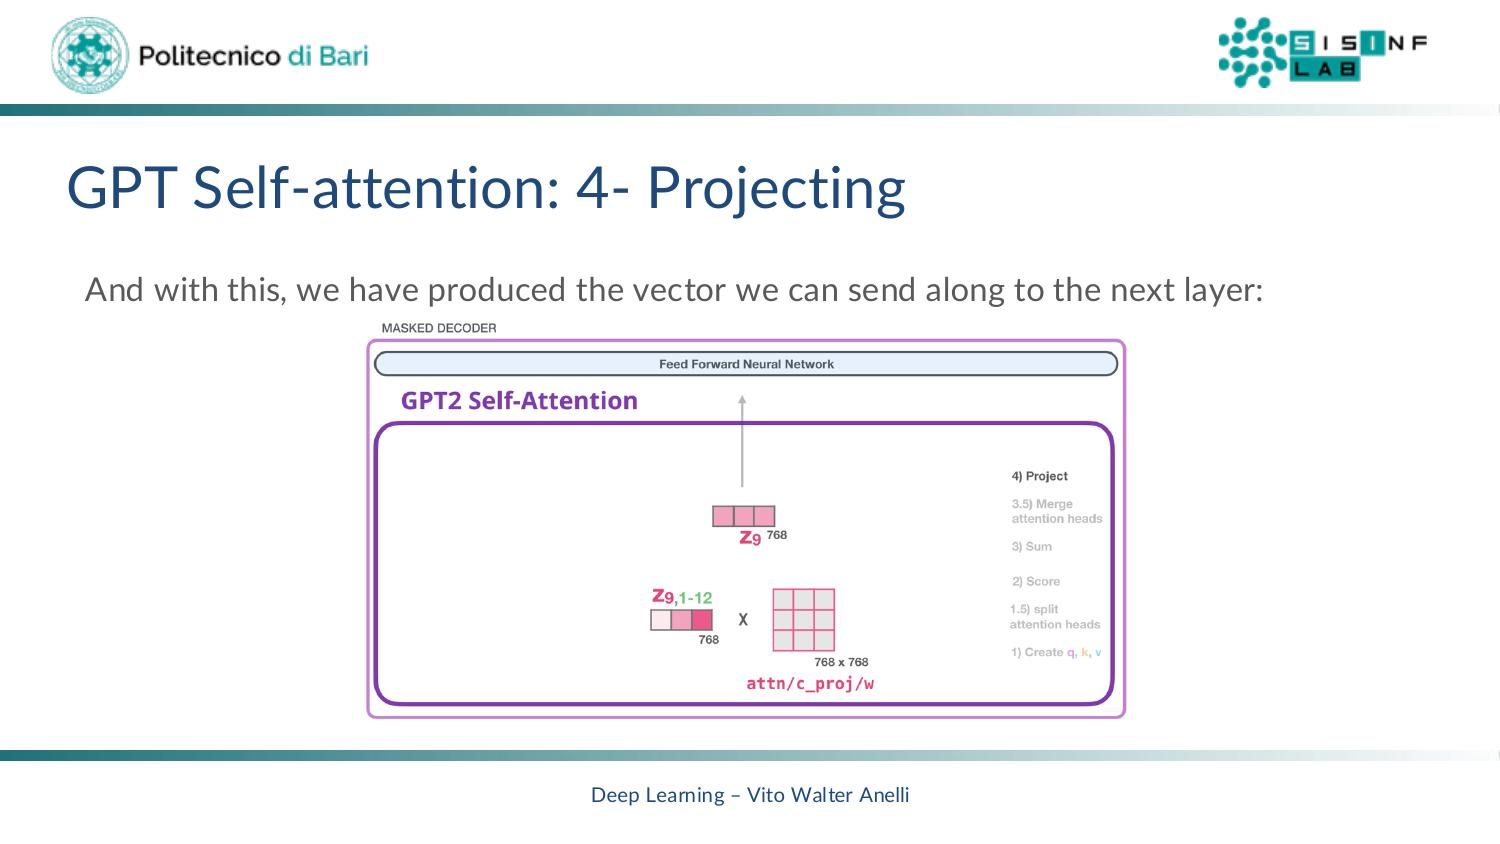
\includegraphics[width=0.70\linewidth]{figures/cf12_19_gpt_projection.jpg}
  \caption{Fase 4: il vettore $Z_{9,1\text{-}12}$ (768 dim,
           concatenazione delle 12 teste) e' proiettato da
           $W^O$ ($768 \times 768$) producendo $Z_9$ (768 dim),
           che passa al FFN del blocco.}
  \label{fig:gpt_proj}
\end{figure}

\subsection{Matrici di Peso in GPT-2 Small}
\label{subsec:gpt2-weights}

\begin{figure}[H]
  \centering
  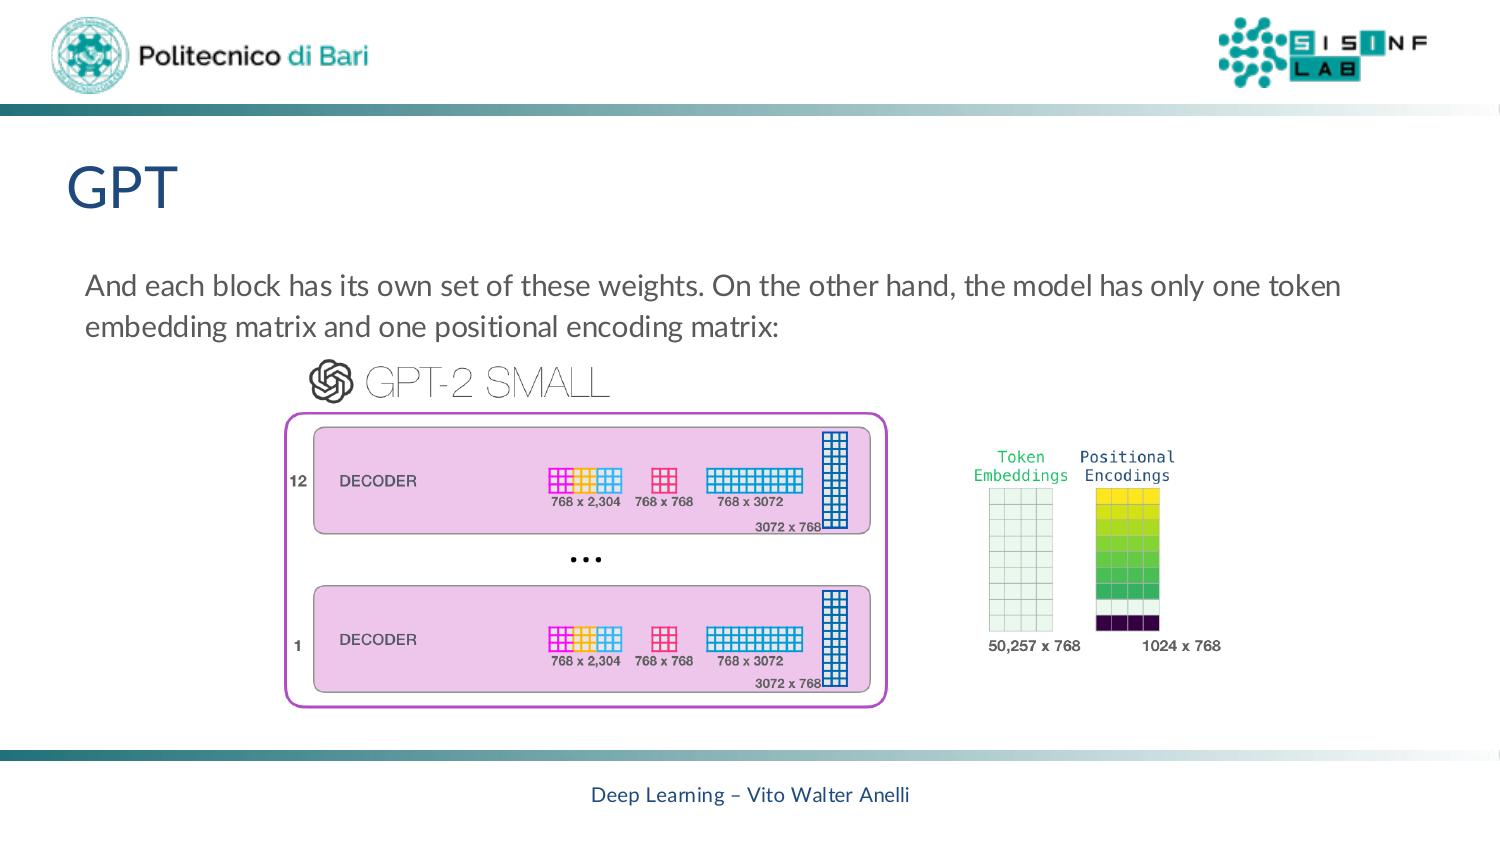
\includegraphics[width=0.88\linewidth]{figures/cf12_20_gpt2_weight_matrices.jpg}
  \caption{Matrici di peso di GPT-2 Small. Ogni decoder block ha:
           $768 \times 2304$ (Q/K/V), $768 \times 768$ (proiezione
           attenzione), $768 \times 3072$ e $3072 \times 768$ (FFN).
           Il modello condivide una sola matrice di token embedding
           ($50257 \times 768$) e una di positional encoding
           ($1024 \times 768$).}
  \label{fig:gpt2_weights}
\end{figure}

Il FFN interno a ogni blocco applica:

\begin{equation}
  \mathrm{FFN}(\mathbf{x})
    = \mathrm{GELU}(\mathbf{x}\,W_1 + b_1)\,W_2 + b_2,
  \label{eq:ffn}
\end{equation}

con $W_1 \in \mathbb{R}^{768 \times 3072}$ e
$W_2 \in \mathbb{R}^{3072 \times 768}$
(dimensione interna $= 4 \times d_{\text{model}}$).

%------------------------------------------------------------
\section{BERT vs.\ GPT: Confronto}
\label{sec:bert-gpt}

\begin{table}[H]
  \centering
  \caption{Confronto tra BERT e GPT.}
  \label{tab:bert-gpt}
  \small
  \begin{tabular}{lll}
    \toprule
    \textbf{Caratteristica} & \textbf{BERT} & \textbf{GPT} \\
    \midrule
    Blocchi usati         & Solo encoder            & Solo decoder \\
    Direzione attenzione  & Bidirezionale           & Causale (sx) \\
    Paradigma             & Fill-in-the-blank (MLM) & Autoregressivo \\
    Pre-training          & MLM + NSP               & Language modeling \\
    Uso principale        & Comprensione (NLU)      & Generazione (NLG) \\
    Autoregressivo        & No                      & Si \\
    \bottomrule
  \end{tabular}
\end{table}

BERT eccelle nei task di comprensione in cui il contesto bilaterale
e' disponibile. GPT e' naturale per la generazione. Architetture
ibride come T5 e BART combinano entrambi gli stack.

%------------------------------------------------------------
\section{Riepilogo delle Componenti}
\label{sec:summary}

\begin{table}[H]
  \centering
  \caption{Componenti principali del Transformer.}
  \label{tab:components}
  \small
  \begin{tabular}{p{4.2cm}p{9cm}}
    \toprule
    \textbf{Componente} & \textbf{Funzione} \\
    \midrule
    Token Embedding
      & Mappa ogni token in $\mathbb{R}^{d_{\text{model}}}$. \\[2pt]
    Positional Encoding
      & Sinusoidi a frequenze diverse; nessun parametro extra. \\[2pt]
    Self-Attention (scalata)
      & $\mathrm{softmax}(QK^\top/\sqrt{d_k})\,V$. \\[2pt]
    Multi-Head Attention
      & $h$ teste in parallelo, concat + proiezione $W^O$. \\[2pt]
    Masked Self-Attention
      & Come SA ma con maschera causale ($-\infty$ per $j > i$). \\[2pt]
    Encoder-Decoder Attention
      & Q dal decoder, K e V dall'encoder. \\[2pt]
    Feed-Forward Network
      & Due layer lineari con GELU, per-posizione. \\[2pt]
    Residual + LayerNorm
      & $\mathrm{LayerNorm}(x + \mathrm{Sublayer}(x))$. \\[2pt]
    Linear + Softmax output
      & Proiezione sul vocabolario e distribuzione di probabilita'. \\
    \bottomrule
  \end{tabular}
\end{table}

%============================================================
%  Capitolo 13 – Diffusion Models
%============================================================
\chapter{Diffusion Models}
\label{ch:diffusion}

I \textbf{modelli di diffusione} (\emph{diffusion models}) rappresentano
la classe di modelli generativi allo stato dell'arte per la sintesi di
immagini ad alta qualità. A differenza delle GAN (Cap.~\ref{ch:gans}),
che apprendono implicitamente la distribuzione dei dati attraverso un
gioco adversariale, i modelli di diffusione apprendono a \emph{invertire}
un processo stocastico di corruzione progressiva dei dati
\citep{bishop2024}. Il modello più noto che sfrutta questa architettura
è \textbf{Stable Diffusion}, un \emph{latent diffusion model} (LDM) che
sposta il processo di diffusione dallo spazio dei pixel a uno spazio
latente compresso, ottenendo un drastico miglioramento dell'efficienza
computazionale.

%------------------------------------------------------------
\section{Stable Diffusion: Architettura Generale}
\label{sec:sd-architecture}

Stable Diffusion è in grado di ricevere come input un \textbf{prompt
testuale} (text-to-image) oppure la combinazione di un testo e
un'immagine di riferimento (text\,+\,image), producendo in uscita
un'immagine sintetica coerente con le indicazioni fornite.

\subsection{Componenti Principali}
\label{subsec:sd-components}

L'architettura di Stable Diffusion è articolata in tre macro-componenti
che operano in sequenza:

\begin{description}
  \item[Text Encoder (CLIPText)] Converte il prompt testuale in una
        sequenza di embedding numerici. Riceve in ingresso fino a 77
        token e produce in uscita 77 vettori di embedding, ciascuno con
        768 dimensioni.
  \item[Image Information Creator (UNet + Scheduler)] È il nucleo del
        modello e il responsabile principale del miglioramento
        qualitativo rispetto ai modelli precedenti. Opera \emph{interamente
        nello spazio latente} e genera iterativamente le informazioni
        sull'immagine attraverso un numero configurabile di passi
        (tipicamente 50 o 100). La sua implementazione tecnica è basata
        su una rete \textbf{UNet} e un \textbf{algoritmo di scheduling}.
  \item[Image Decoder (Autoencoder Decoder)] Converte il tensore di
        informazioni latenti elaborato nella corrispondente immagine
        nello spazio dei pixel. Riceve in ingresso un tensore di
        dimensioni $(4, 64, 64)$ e produce un'immagine di dimensioni
        $(3, 512, 512)$, corrispondenti ai canali
        (rosso/verde/blu, larghezza, altezza).
\end{description}

\begin{figure}[H]
  \centering
  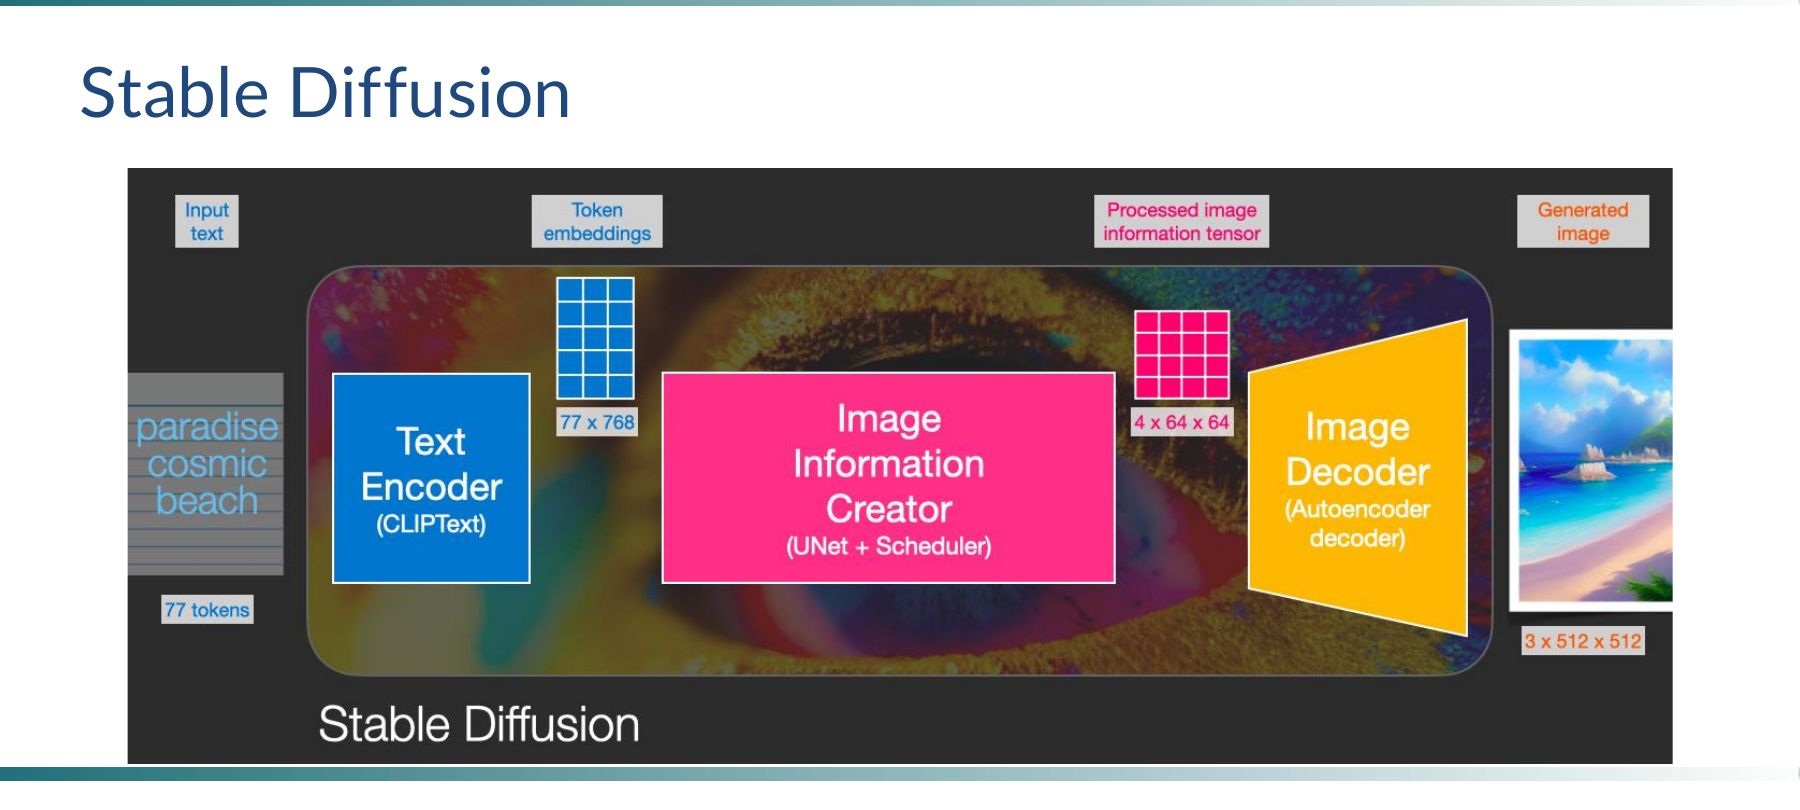
\includegraphics[width=0.92\linewidth]{figures/cf13_sd_full_pipeline.png}
  \caption{Architettura di Stable Diffusion. Il testo in ingresso
           viene prima codificato dal \emph{Text Encoder} (CLIPText)
           in 77 token embedding di dimensione 768. L'\emph{Image
           Information Creator} (UNet + Scheduler) opera nello spazio
           latente producendo un tensore $4\times64\times64$, che viene
           infine decodificato dall'\emph{Image Decoder} (autoencoder
           decoder) nell'immagine finale $3\times512\times512$.}
  \label{fig:sd_components}
\end{figure}

Il processo complessivo si divide in tre fasi numerate:
\begin{enumerate}
  \item Il \textbf{Text Encoder} converte i 77 token di input negli
        embedding testuali.
  \item L'\textbf{Image Information Creator} riceve gli embedding
        testuali e un tensore di rumore casuale, e li elabora
        attraverso la diffusione latente.
  \item L'\textbf{Image Decoder} traduce il tensore latente elaborato
        nell'immagine generata.
\end{enumerate}

%------------------------------------------------------------
\section{Il Processo di Diffusione}
\label{sec:diffusion-process}

\subsection{Forward Diffusion: Corruzione con Rumore}
\label{subsec:forward-diffusion}

Il \textbf{processo di diffusione in avanti} (\emph{forward diffusion})
consiste nel costruire il dataset di addestramento del predittore del
rumore. Dato un'immagine del dataset, si generano esempi di
addestramento secondo lo schema seguente:

\begin{enumerate}
  \item Si seleziona un'immagine dal dataset di addestramento.
  \item Si genera un campione di rumore casuale.
  \item Si seleziona una quantità di rumore da aggiungere.
  \item Si aggiunge il rumore all'immagine nella quantità stabilita.
\end{enumerate}

Poiché la quantità di rumore è controllabile con precisione, è possibile
creare decine di esempi di addestramento per ogni immagine, distribuendo
la corruzione su decine di passi discreti.

\subsection{Addestramento del Predittore del Rumore}
\label{subsec:noise-predictor-training}

Il dataset così costruito, in cui ogni esempio è composto da
(immagine corrotta, quantità di rumore aggiunta, campione di rumore
effettivo), viene utilizzato per addestrare un modello denominato
\textbf{Noise Predictor}, implementato come rete \textbf{UNet}.
Un singolo passo di addestramento comprende:

\begin{enumerate}
  \item Selezionare un esempio di addestramento dal dataset.
  \item Far predire alla UNet il campione di rumore contenuto
        nell'immagine.
  \item Calcolare la \emph{loss} confrontando la previsione con il
        rumore effettivo.
  \item Aggiornare i pesi del modello tramite backpropagation.
\end{enumerate}

\subsection{Reverse Diffusion: Rimozione Iterativa del Rumore}
\label{subsec:reverse-diffusion}

Una volta addestrato, il \emph{Noise Predictor} è in grado di stimare
il rumore contenuto in un'immagine rumorosa. La generazione di nuove
immagini sfrutta la \textbf{diffusione inversa} (\emph{reverse
diffusion}):

\begin{enumerate}
  \item Si genera un tensore completamente casuale (rumore puro).
  \item Il predittore del rumore stima il rumore presente.
  \item Il rumore stimato viene sottratto dal tensore corrente,
        ottenendo un'immagine leggermente de-rumorata.
  \item I passi 2 e 3 vengono ripetuti per un numero fissato di
        iterazioni di campionamento.
\end{enumerate}

Ripetendo questo processo, l'immagine ``emerge'' progressivamente dal
rumore. Se il dataset di addestramento era composto da immagini
esteticamente pregevoli (ad esempio LAION Aesthetics, su cui è stato
addestrato Stable Diffusion), l'immagine generata tenderà ad essere
anch'essa esteticamente pregevole. Il risultato finale dipende dunque
direttamente dalla natura del dataset di addestramento: un modello
addestrato su loghi produrrà loghi, uno addestrato su fotografie
produrrà fotografie.

\begin{figure}[H]
  \centering
  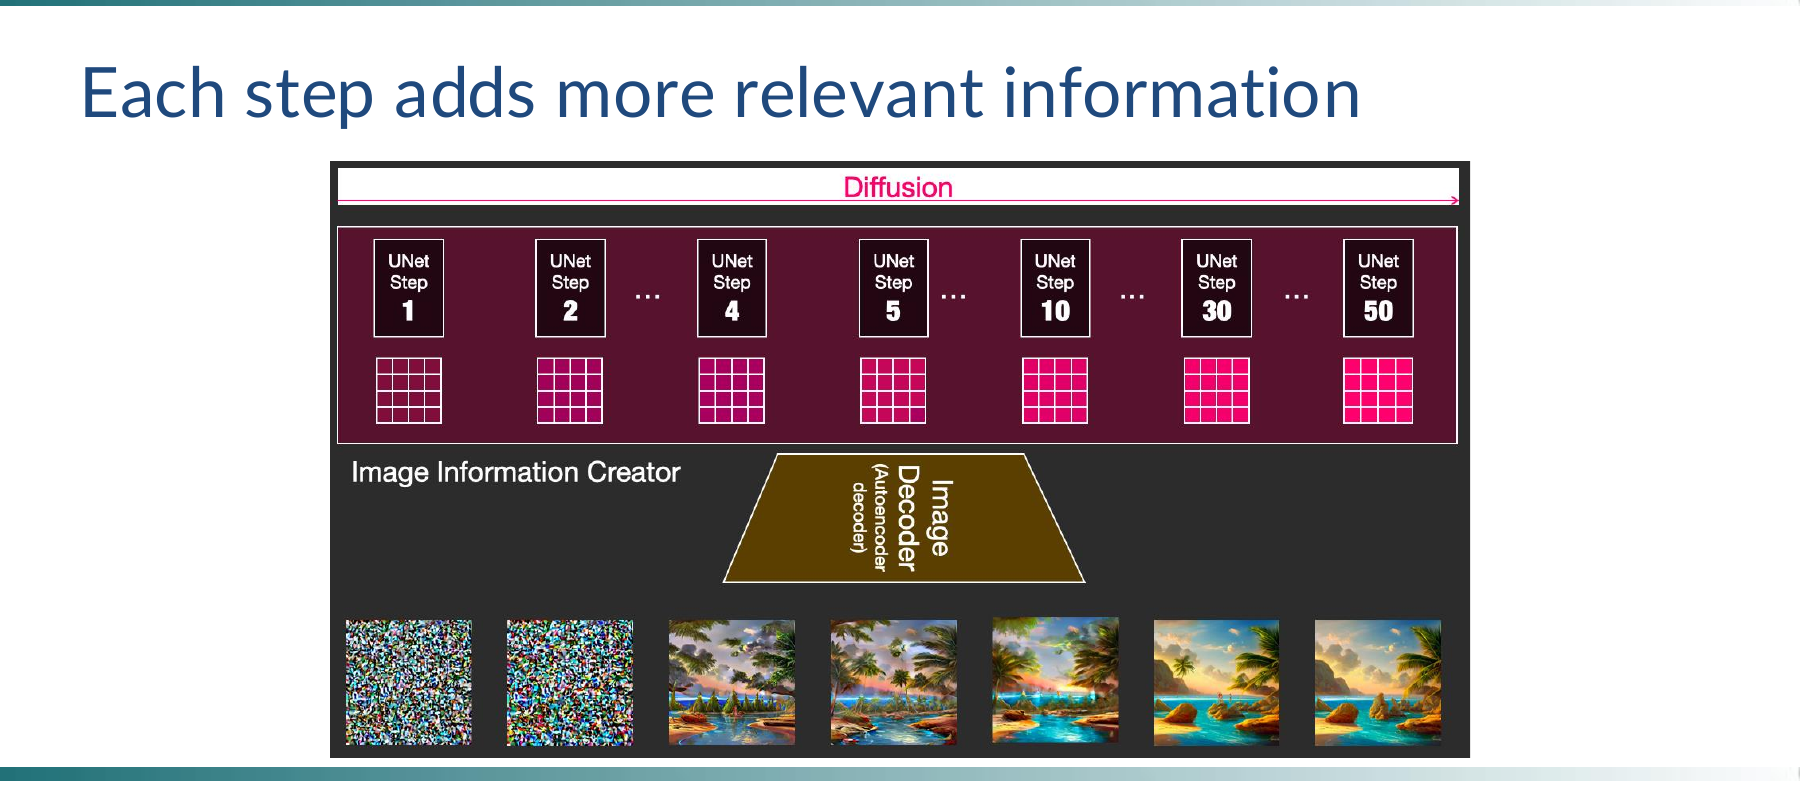
\includegraphics[width=0.90\linewidth]{figures/cf13_reverse_diffusion_steps.png}
  \caption{Processo di diffusione inversa. Partendo da un tensore
           di rumore puro (in basso a sinistra), il predittore del
           rumore (UNet) sottrae iterativamente il rumore stimato.
           A ogni passo si ottiene un'immagine via via più pulita,
           fino all'immagine finale generata (in basso a destra).}
  \label{fig:reverse_diffusion}
\end{figure}

\subsection{Noise Schedule}
\label{subsec:noise-schedule}

Il passaggio dall'immagine rumorosa a quella pulita avviene attraverso
una progressione definita dal \textbf{noise schedule}. Il noise schedule
specifica la quantità attesa di rumore residuo a ciascun passo di
campionamento e può essere configurato liberamente:

\begin{itemize}
  \item Si può scegliere di rimuovere la stessa quantità di rumore
        a ogni passo (\emph{uniform schedule}).
  \item Si può rimuovere più rumore nelle fasi iniziali del processo
        (\emph{decaying schedule}).
\end{itemize}

In ciascun passo il \textbf{sampler} sottrae esattamente la quantità
di rumore necessaria per raggiungere il livello atteso dal noise schedule
al passo successivo.

%------------------------------------------------------------
\section{Latent Diffusion: Diffusione nello Spazio Compresso}
\label{sec:latent-diffusion}

\subsection{Motivazione: Limiti della Diffusione nello Spazio dei Pixel}
\label{subsec:pixel-space-limits}

L'esecuzione del processo di diffusione direttamente nello \textbf{spazio
dei pixel} presenta limitazioni computazionali severe. Un'immagine
$512 \times 512$ con tre canali colore (rosso, verde, blu) occupa uno
spazio di $786\,432$ dimensioni: per ogni immagine è necessario
specificare quel numero di valori. Modelli come \textbf{Google Imagen}
e \textbf{OpenAI DALL-E} operano nello spazio dei pixel e, pur
adottando alcune ottimizzazioni, rimangono computazionalmente costosi e
non eseguibili su una singola GPU di consumo.

\subsection{Spazio Latente e Variational Autoencoder}
\label{subsec:latent-space-vae}

Stable Diffusion risolve questo problema spostando l'intero processo di
diffusione in uno \textbf{spazio latente} compresso, 48 volte più piccolo
dello spazio dei pixel. Questo approccio è reso possibile dalla
\textbf{manifold hypothesis}: le immagini naturali non sono casuali,
ma presentano un'alta regolarità strutturale (un viso segue specifiche
relazioni spaziali tra occhi, naso, guance e bocca; un cane ha quattro
zampe e una forma caratteristica). L'alta dimensionalità dello spazio
dei pixel è quindi in larga misura \emph{artificiale}: le immagini
naturali possono essere compresse nello spazio latente senza perdita
significativa di informazione \citep{bishop2024}.

La compressione e la successiva ricostruzione sono delegate a un
\textbf{Variational Autoencoder} (VAE), composto da:

\begin{description}
  \item[Encoder] Comprime l'immagine dallo spazio dei pixel
        $(3, 512, 512)$ alla rappresentazione latente $(4, 64, 64)$.
  \item[Decoder] Ricostruisce l'immagine dalla rappresentazione latente
        allo spazio dei pixel.
\end{description}

\begin{figure}[H]
  \centering
  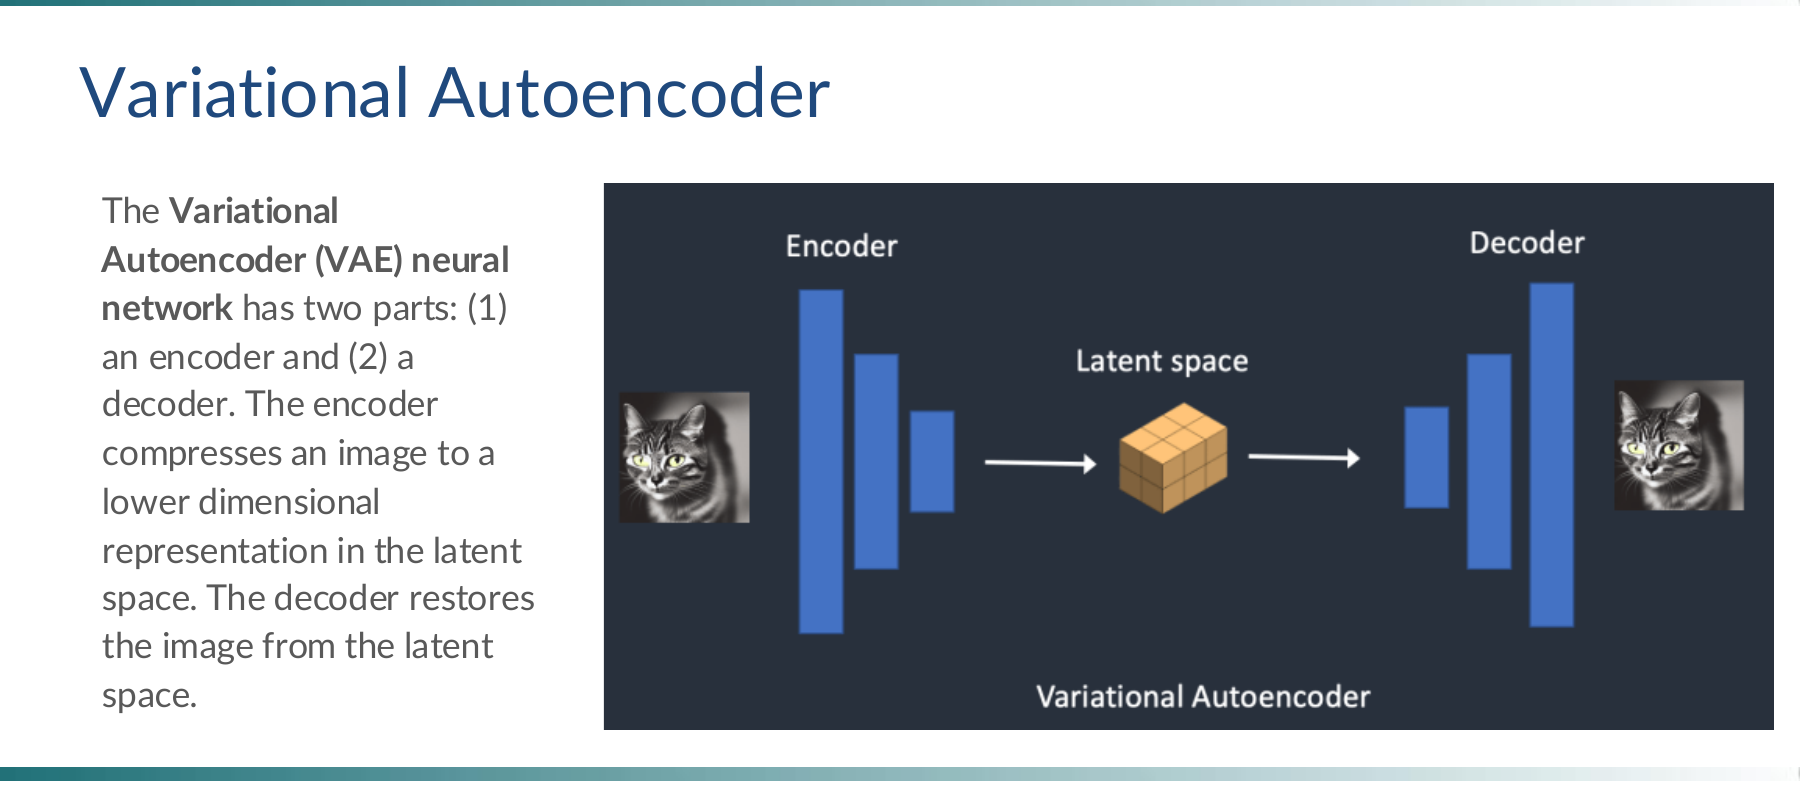
\includegraphics[width=0.88\linewidth]{figures/cf13_vae.png}
  \caption{Variational Autoencoder (VAE) utilizzato in Stable Diffusion.
           L'\emph{encoder} comprime l'immagine nello spazio latente
           $(4\times64\times64)$; il \emph{decoder} la ricostruisce
           nello spazio dei pixel $(3\times512\times512)$.}
  \label{fig:vae}
\end{figure}

\subsection{Addestramento e Inferenza Latente}
\label{subsec:latent-training-inference}

Durante l'\textbf{addestramento}, il processo di diffusione in avanti
opera direttamente sulle rappresentazioni latenti:

\begin{enumerate}
  \item L'immagine originale viene codificata nell'encoder VAE, ottenendo
        il corrispondente tensore latente.
  \item Vengono generati esempi di addestramento aggiungendo quantità
        variabili di rumore al tensore latente (non all'immagine pixel).
  \item Il Noise Predictor (UNet) viene addestrato a predire il rumore
        aggiunto nella rappresentazione latente.
\end{enumerate}

Durante l'\textbf{inferenza} (generazione), la diffusione inversa viene
eseguita interamente nello spazio latente:

\begin{enumerate}
  \item Si genera un tensore latente casuale.
  \item Il Noise Predictor stima il rumore del tensore latente.
  \item Il rumore stimato viene sottratto dal tensore latente.
  \item I passi 2 e 3 vengono ripetuti per il numero di passi di
        campionamento prescelti.
  \item Il decoder VAE converte il tensore latente finale nell'immagine
        generata.
\end{enumerate}

\paragraph{Nota sulla risoluzione.} La dimensione del tensore latente
è direttamente proporzionale alla risoluzione dell'immagine: per
immagini $512\times512$ il latente è $4\times64\times64$, mentre per
un'immagine ritratto $768\times512$ è $4\times96\times64$. Poiché
Stable Diffusion v1 è stato ottimizzato su immagini $512\times512$,
generare immagini di dimensioni superiori può produrre artefatti
(ad esempio oggetti duplicati).

%------------------------------------------------------------
\section{Condizionamento Testuale}
\label{sec:text-conditioning}

\subsection{Dalla Diffusione Non Condizionata al Condizionamento}
\label{subsec:conditioning-intro}

Il processo di diffusione inversa descritto finora è \textbf{non
condizionato}: il modello genera immagini casuali senza possibilità
di controllo sul contenuto. Per ottenere un modello \emph{text-to-image}
è necessario introdurre il \textbf{condizionamento}, ossia un meccanismo
che guidi il predittore del rumore affinché le immagini generate siano
coerenti con il prompt testuale.

\subsection{Text Encoder: CLIP}
\label{subsec:clip}

La componente di codifica testuale di Stable Diffusion è basata su
\textbf{CLIP} (\emph{Contrastive Language–Image Pre-training}), un
modello pre-addestrato su 400 milioni di coppie immagine--didascalia
raccolte dal Web (tramite i tag \texttt{alt} delle immagini).

CLIP è composto da due encoder:
\begin{description}
  \item[Image Encoder] Mappa immagini in uno spazio di embedding.
  \item[Text Encoder] Mappa testi nello stesso spazio di embedding.
\end{description}

L'addestramento avviene per \textbf{contrasto}: dato un mini-batch di
coppie (immagine, didascalia), CLIP massimizza la \emph{cosine
similarity} tra gli embedding di coppie corrispondenti e la minimizza
tra coppie non corrispondenti. Al termine dell'addestramento, embedding
di immagini e testi semanticamente simili si trovano in regioni vicine
dello spazio.

Il prompt testuale viene elaborato come segue:
\begin{enumerate}
  \item Un \textbf{tokenizer} converte ogni parola del prompt in un
        token numerico (ad esempio: ``photo'' $\to$ 50, ``cat'' $\to$
        239).
  \item Ogni token viene convertito in un vettore di embedding a 768
        valori.
  \item Gli embedding vengono processati dal \textbf{text transformer},
        che produce la sequenza finale di 77 vettori pronti per essere
        consumati dal Noise Predictor.
\end{enumerate}

\paragraph{Importanza della scelta del language model.} Il paper di
Google Imagen ha dimostrato sperimentalmente che la qualità del
modello linguistico utilizzato come encoder testuale ha un impatto
maggiore sulla qualità delle immagini generate rispetto alla dimensione
dei componenti di generazione dell'immagine. Per questo motivo Stable
Diffusion v2 ha adottato \textbf{OpenCLIP}, una variante open-source
di CLIP con modelli testuali fino a 354M parametri (contro i 63M di
CLIPText usato in v1), migliorando la qualità delle immagini generate.

\subsection{Cross-Attention: Integrazione del Testo nella UNet}
\label{subsec:cross-attention}

Il condizionamento testuale viene integrato nel Noise Predictor attraverso
un meccanismo di \textbf{cross-attention} inserito tra i blocchi ResNet
della UNet. I blocchi ResNet non accedono direttamente al testo:
i layer di cross-attention fondono le rappresentazioni testuali nello
spazio latente, consentendo ai blocchi ResNet successivi di sfruttare
tale informazione nel proprio processing.

Il \textbf{meccanismo di cross-attention} è un'estensione dell'attenzione
del Transformer che combina due sequenze di embedding distinte. A
differenza della \emph{self-attention}, che opera su una singola
sequenza, la cross-attention riceve:

\begin{itemize}
  \item Una sequenza $S_1$ (il condizionamento, ad esempio gli embedding
        testuali), da cui si derivano le matrici \textbf{Key} ($K$) e
        \textbf{Value} ($V$).
  \item Una sequenza $S_2$ (lo stato latente corrente), da cui si derivano
        le \textbf{Query} ($Q$).
\end{itemize}

Il calcolo segue la formula standard dell'attenzione scalata:
\begin{equation}
  \mathrm{CrossAttention}(S_1, S_2)
  \;=\;
  \mathrm{softmax}\!\left(
    \frac{(W_Q S_2)(W_K S_1)^\top}{\sqrt{d_k}}
  \right) W_V S_1
  \label{eq:cross-attention}
\end{equation}
dove $W_Q$, $W_K$, $W_V$ sono matrici di proiezione apprese, e $d_k$
è la dimensione delle chiavi. L'output ha la stessa dimensione e lunghezza
della sequenza $S_2$ (lo stato latente).

\begin{figure}[H]
  \centering
  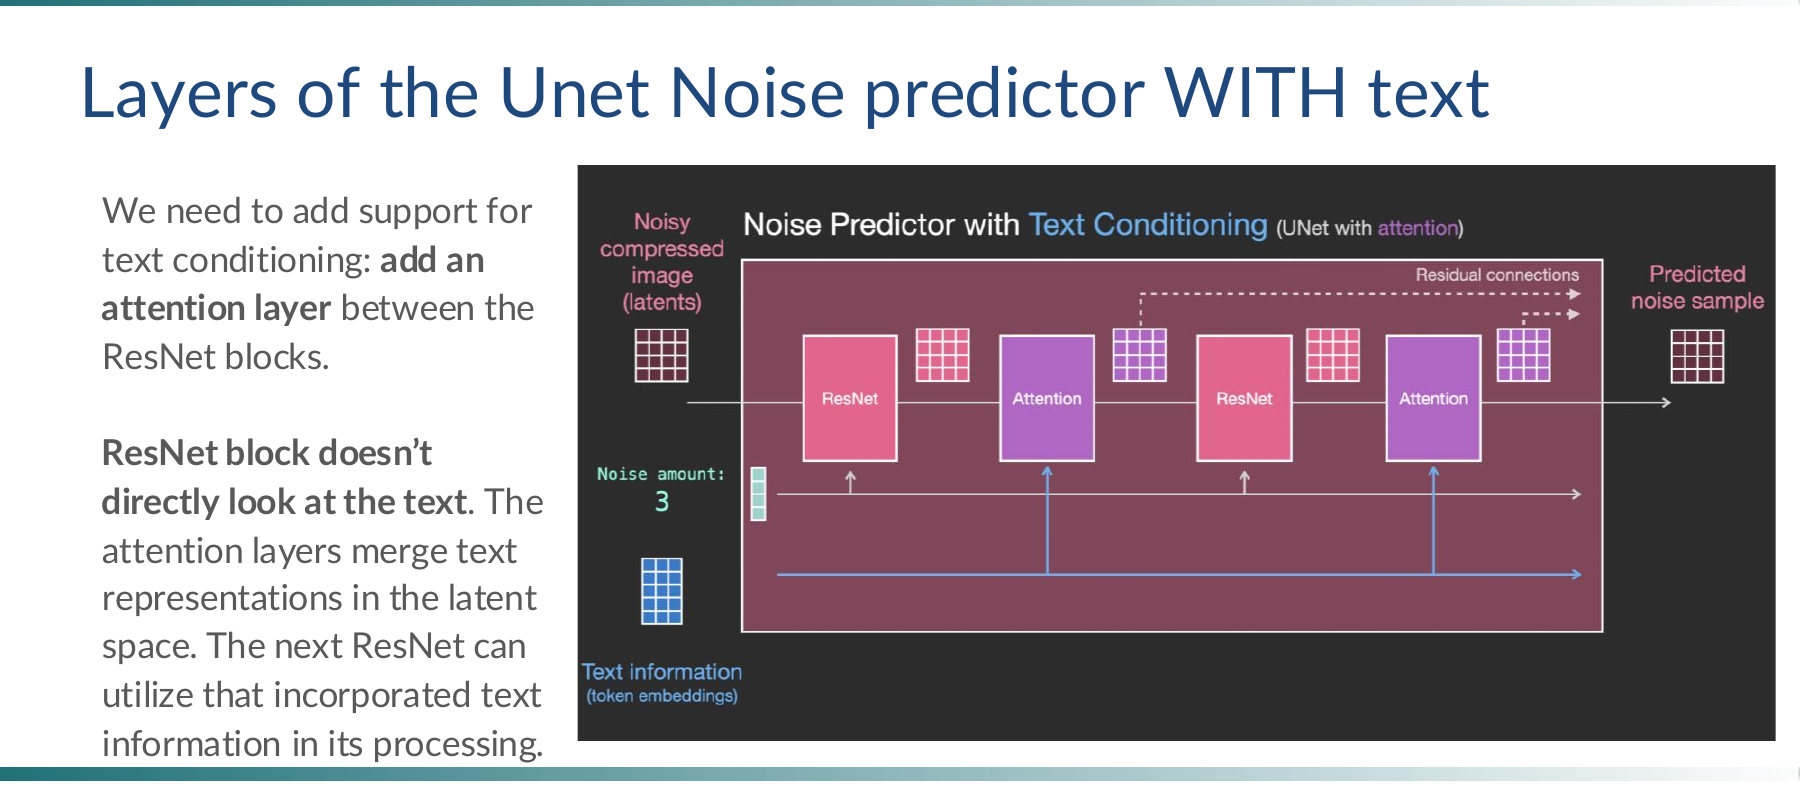
\includegraphics[width=0.88\linewidth]{figures/cf13_unet_with_attention.png}
  \caption{Struttura interna del Noise Predictor (UNet) con
           condizionamento testuale. I blocchi \emph{ResNet} processano
           il tensore latente; i layer di \emph{Attention} fondono
           la rappresentazione testuale nello spazio latente tramite
           cross-attention. Le connessioni residuali collegano le
           rappresentazioni intermedie alle parti più profonde della rete.}
  \label{fig:unet_attention}
\end{figure}

\begin{figure}[H]
  \centering
  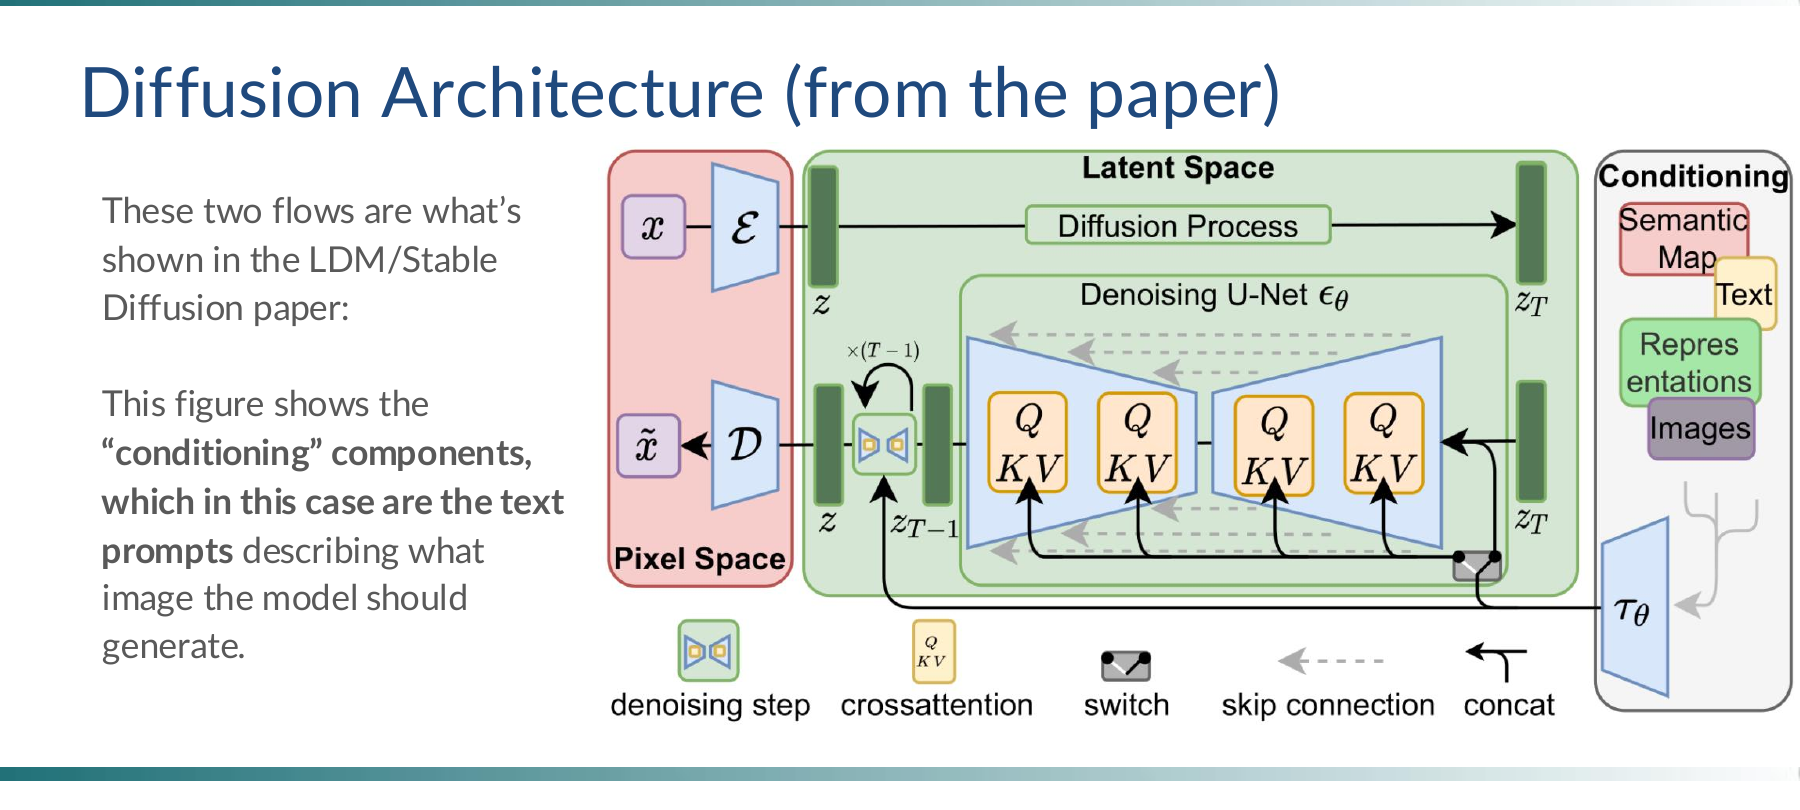
\includegraphics[width=0.92\linewidth]{figures/cf13_ldm_architecture.png}
  \caption{Architettura del Latent Diffusion Model (LDM) dal paper originale.
           L'encoder $\mathcal{E}$ comprime l'immagine nello spazio latente;
           la denoising UNet $\epsilon_\theta$ opera su tale spazio attraverso
           moduli di cross-attention ($Q$/$K$/$V$) che integrano il
           condizionamento $\tau_\theta$ (testo, mappe semantiche, immagini);
           il decoder $\mathcal{D}$ ricostruisce l'immagine nello spazio pixel.}
  \label{fig:ldm_architecture}
\end{figure}

\paragraph{Esempio: self-attention e cross-attention nel prompt.}
Considerando il prompt ``A man with blue eyes'': Stable Diffusion
sfrutta la \emph{self-attention} all'interno del prompt per associare
i token ``blue'' ed ``eyes'', generando un uomo con gli occhi blu e
non una camicia blu. Successivamente, la \emph{cross-attention} tra
prompt e immagine guida il processo di diffusione inversa verso immagini
contenenti occhi blu.

%------------------------------------------------------------
\section{Classifier-Free Guidance (CFG)}
\label{sec:cfg}

\subsection{Classifier Guidance}
\label{subsec:classifier-guidance}

Il \textbf{classifier guidance} è una tecnica che incorpora etichette
di classe nel processo di diffusione, guidando la generazione verso
immagini appartenenti a una categoria specifica (ad esempio ``gatto'').
La \emph{classifier guidance scale} controlla quanto strettamente il
processo di diffusione deve seguire l'etichetta:
\begin{itemize}
  \item Con una scala \textbf{bassa}, i campioni generati coprono
        un'ampia porzione della distribuzione della categoria.
  \item Con una scala \textbf{alta}, i campioni sono fortemente
        vincolati alle caratteristiche più tipiche e non ambigue della
        categoria, a scapito della diversità.
\end{itemize}

\subsection{Classifier-Free Guidance}
\label{subsec:cfg}

Sebbene il classifier guidance abbia ottenuto risultati eccellenti,
richiede un modello classificatore separato, il che complica
l'addestramento. Il \textbf{Classifier-Free Guidance} (CFG) risolve
questo problema incorporando la guida direttamente nel Noise Predictor,
senza la necessità di un classificatore esterno. Invece di etichette
di classe, il condizionamento avviene tramite \textbf{didascalie
testuali} e un modello di diffusione condizionato, esattamente come
nel paradigma text-to-image.

La \textbf{CFG scale} è il parametro che controlla l'intensità del
condizionamento:
\begin{itemize}
  \item Con CFG scale pari a \textbf{0}, la generazione è non
        condizionata (il prompt viene ignorato).
  \item Con valori \textbf{crescenti}, il processo di diffusione
        viene guidato sempre più strettamente verso il prompt testuale,
        producendo immagini più fedeli ma meno variate.
\end{itemize}

%------------------------------------------------------------
\section{Modalità di Generazione Avanzate}
\label{sec:advanced-modes}

\subsection{Image-to-Image}
\label{subsec:img2img}

Il metodo \textbf{image-to-image} (\emph{SDEdit}) estende la generazione
text-to-image ricevendo in input sia un prompt testuale sia un'immagine
di riferimento. L'immagine generata è condizionata da entrambi gli input.
Il processo si articola come segue:

\begin{enumerate}
  \item L'immagine di input viene codificata nello spazio latente
        tramite l'encoder VAE.
  \item Viene aggiunto rumore al tensore latente. Il parametro
        \textbf{denoising strength} controlla la quantità di rumore:
        con 0 non viene aggiunto rumore, con 1 viene aggiunto il
        massimo (il tensore diventa completamente casuale).
  \item Il Noise Predictor (UNet) riceve il tensore latente rumoroso
        e il prompt testuale, e predice il rumore nello spazio latente.
  \item Il rumore predetto viene sottratto dal tensore latente.
  \item I passi 3 e 4 vengono ripetuti per il numero prefissato di
        passi di campionamento.
  \item Il decoder VAE converte il tensore latente finale nell'immagine
        generata.
\end{enumerate}

\subsection{Inpainting}
\label{subsec:inpainting}

L'\textbf{inpainting} è un caso particolare di image-to-image in cui
il rumore viene aggiunto esclusivamente alle regioni dell'immagine che
si intende modificare. La quantità di rumore è controllata, anche in
questo caso, dal parametro di \emph{denoising strength}.

\subsection{Depth-to-Image}
\label{subsec:depth2img}

Il metodo \textbf{depth-to-image} estende l'image-to-image con un
condizionamento aggiuntivo basato su una \textbf{mappa di profondità}.
La mappa viene stimata automaticamente dall'immagine di input tramite
il modello \textbf{MiDaS} e viene fornita come ulteriore condizionamento
al Noise Predictor nella fase di predizione del rumore.

\subsection{Altri Condizionamenti: ControlNet}
\label{subsec:controlnet}

Il prompt testuale non è l'unico modo per condizionare un modello di
diffusione. \textbf{ControlNet} condiziona il Noise Predictor con
contorni rilevati automaticamente, pose umane stimate, mappe di
segmentazione e altri segnali strutturali, ottenendo un controllo
preciso sulla composizione delle immagini generate.

%------------------------------------------------------------
\section{Stable Diffusion v1 vs.\ v2}
\label{sec:sd-v1-v2}

\subsection{Differenze nel Modello}
\label{subsec:v1v2-model}

La principale differenza architetturale tra le due versioni riguarda
il \textbf{text encoder}:

\begin{itemize}
  \item \textbf{Stable Diffusion v1} utilizza \textbf{CLIP ViT-L/14}
        di OpenAI (63M parametri).
  \item \textbf{Stable Diffusion v2} utilizza \textbf{OpenCLIP},
        una variante open-source con modelli testuali fino a
        354M parametri (circa 5 volte più grande).
\end{itemize}

Il passaggio a OpenCLIP migliora la qualità delle immagini (modelli
linguistici più grandi migliorano le prestazioni generative) e offre
maggiore trasparenza al mondo della ricerca, poiché il training data
è pubblicamente documentato.

\subsection{Differenze nei Dati di Addestramento}
\label{subsec:v1v2-data}

\paragraph{Stable Diffusion v1.4} è stato addestrato su:
\begin{itemize}
  \item 237k passi a risoluzione $256\times256$ sul dataset
        \texttt{laion2B-en}.
  \item 194k passi a risoluzione $512\times512$ su
        \texttt{laion-high-resolution}.
  \item 225k passi a $512\times512$ su \texttt{laion-aesthetics v2 5+},
        con il 10\% di \emph{dropping} del condizionamento testuale.
\end{itemize}

\paragraph{Stable Diffusion v2.0} è stato addestrato su un sottoinsieme
di \texttt{LAION-5B} filtrato per contenuti espliciti (con classificatore
LAION-NSFW, $p_\text{unsafe}=0.1$, score estetico $\geq 4.5$):
\begin{itemize}
  \item 550k passi a $256\times256$.
  \item 850k passi a $512\times512$ su immagini con risoluzione
        $\geq 512\times512$.
  \item 150k passi con un \emph{v-objective}.
  \item 140k passi aggiuntivi a $768\times768$.
\end{itemize}

\paragraph{Stable Diffusion v2.1} è un fine-tuning di v2.0:
\begin{itemize}
  \item 55k passi aggiuntivi con $p_\text{unsafe}=0.1$.
  \item 155k passi con $p_\text{unsafe}=0.98$ (filtro NSFW
        sostanzialmente disattivato nelle ultime fasi).
\end{itemize}

\subsection{Differenze nelle Prestazioni}
\label{subsec:v1v2-perf}

Gli utenti riscontrano in v2 una minore capacità di controllare lo stile
artistico e di riprodurre celebrity rispetto a v1. Questo è probabilmente
dovuto alla differenza nei dati di addestramento: il dataset proprietario
di OpenAI su cui è stato addestrato CLIP ViT-L/14 contiene verosimilmente
più opere d'arte e fotografie di personaggi noti.

%------------------------------------------------------------
\section{Confronto con le GAN e con altri Modelli Generativi}
\label{sec:diffusion-vs-gans}

I modelli di diffusione hanno in larga misura superato le GAN in termini
di qualità generativa, in particolare per:

\begin{itemize}
  \item \textbf{Diversità dei campioni}: assenza del mode collapse,
        tipico delle GAN.
  \item \textbf{Stabilità dell'addestramento}: il processo di
        addestramento basato su una semplice loss di predizione del
        rumore è molto più stabile rispetto al gioco adversariale.
  \item \textbf{Qualità delle immagini}: campioni ad alta fedeltà
        con struttura semantica coerente, grazie al condizionamento
        testuale tramite cross-attention.
\end{itemize}

Il principale svantaggio rimane la \textbf{lentezza dell'inferenza}:
la generazione richiede decine o centinaia di passi di denoising, mentre
una GAN genera un campione in un singolo passaggio forward.

\begin{table}[H]
  \centering
  \caption{Confronto tra modelli generativi principali.}
  \label{tab:diffusion-comparison}
  \small
  \begin{tabular}{lllll}
    \toprule
    \textbf{Modello} & \textbf{Spazio di lavoro}
      & \textbf{Qualità} & \textbf{Diversità} & \textbf{Criticità} \\
    \midrule
    GAN
      & Pixel / latente
      & Alta
      & Bassa (mode collapse)
      & Instabilità, mode collapse \\
    VAE
      & Latente
      & Media
      & Alta
      & Campioni sfocati \\
    Normalizing Flow
      & Biiezione
      & Alta
      & Alta
      & Architettura vincolata \\
    Diffusion (pixel)
      & Pixel
      & Molto alta
      & Alta
      & Inferenza molto lenta \\
    Latent Diffusion
      & Latente
      & Molto alta (SOTA)
      & Alta
      & Inferenza lenta \\
    \bottomrule
  \end{tabular}
\end{table}

\paragraph{Considerazioni pratiche.}
\begin{enumerate}
  \item Il parametro \textbf{steps} (numero di passi UNet) è il
        principale trade-off qualità/velocità: più passi producono
        immagini migliori ma tempi di generazione più lunghi.
  \item La \textbf{CFG scale} controlla il bilanciamento tra fedeltà
        al prompt e diversità: valori tipici sono nell'intervallo 7--12.
  \item Il parametro \textbf{denoising strength} in image-to-image
        determina quanto l'immagine di output si discosterà da quella
        di input.
  \item In Stable Diffusion v1, è consigliabile mantenere almeno un
        lato dell'immagine a 512 pixel e usare un \emph{AI upscaler}
        per risoluzioni superiori, per evitare artefatti dovuti alla
        fuori distribuzione.
  \item I \textbf{VAE files} (decoder fine-tunati) possono essere
        utilizzati in Stable Diffusion v1 per migliorare la resa di
        occhi e volti, poiché la compressione VAE comporta una perdita
        di dettagli fini che il decoder specializzato è in grado di
        recuperare.
\end{enumerate}

%============================================================
%  Capitolo 14 – Graph Neural Networks e Graph Convolutional Networks
%============================================================
\chapter{Graph Neural Networks}
\label{ch:gnn}

I \textbf{Graph Neural Networks} (GNN) sono una famiglia di modelli di
deep learning progettati per operare su dati strutturati come grafi.
A differenza di CNN e RNN, che assumono rispettivamente una griglia
regolare o una sequenza ordinata, le GNN sono in grado di gestire
strutture di connettività arbitrarie, sfruttando la topologia del
grafo per apprendere rappresentazioni ricche di nodi, archi e del
grafo nel suo insieme \citep{bishop2024}.

%------------------------------------------------------------
\section{Grafi come Strutture Dati}
\label{sec:graphs}

\subsection{Definizione e Attributi}
\label{subsec:graph-def}

Un \textbf{grafo} $G = (V, E)$ è una struttura dati composta da nodi
(vertici) e archi, privi di un inizio o una fine definiti. I grafi
possono essere \emph{diretti} (la direzione della connessione è
rilevante) o \emph{indiretti} (l'ordine non conta). I grafi diretti
possono essere unidirezionali o bidirezionali.

Ogni grafo è caratterizzato da tre tipi di attributi:

\begin{description}
  \item[$V$ — Vertex attributes] Attributi associati a ciascun nodo,
        ad esempio l'identità del nodo o il numero di vicini.
  \item[$E$ — Edge attributes] Attributi associati a ciascun arco,
        incluse la direzione, il peso o l'identità dell'arco.
  \item[$U$ — Global attributes] Attributi globali dell'intero grafo,
        detti anche \emph{master node} o \emph{context vector},
        ad esempio il numero totale di nodi o il cammino più lungo.
\end{description}

\begin{figure}[H]
  \centering
  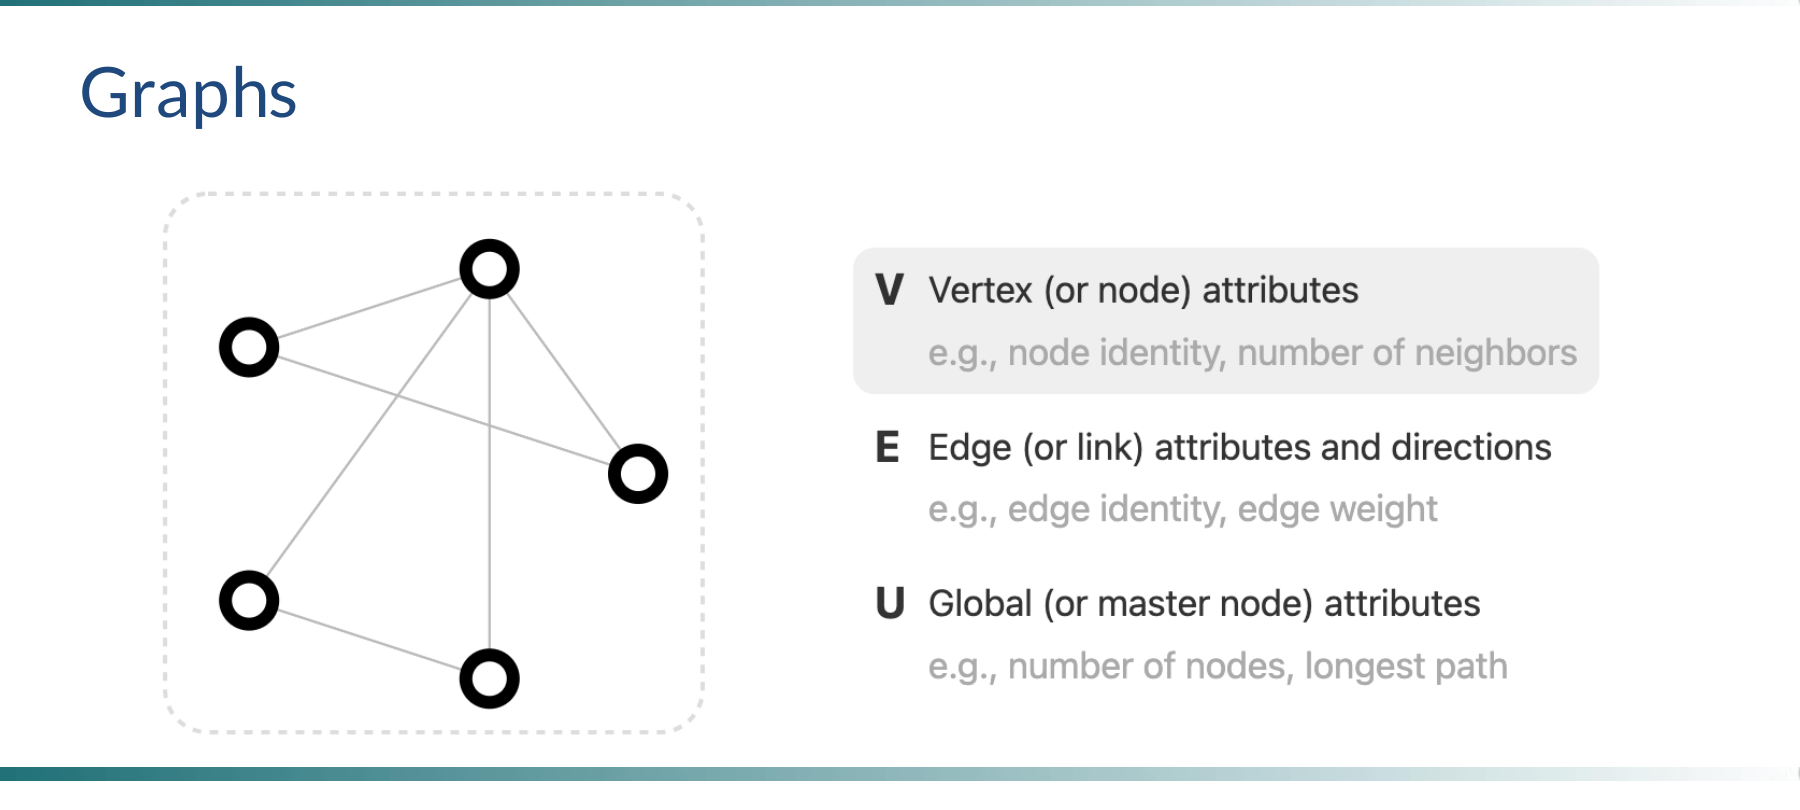
\includegraphics[width=0.82\linewidth]{figures/cf14_graph_attributes.png}
  \caption{Un grafo con i tre tipi di attributi: $V$ (nodi),
           $E$ (archi) e $U$ (globale). I nodi memorizzano
           proprietà locali, gli archi codificano relazioni,
           il vettore globale riassume proprietà dell'intero grafo.}
  \label{fig:graph_attributes}
\end{figure}

\subsection{Grafi in Natura: Esempi di Dominio}
\label{subsec:graph-examples}

I grafi modellano naturalmente numerosi tipi di dati reali:

\begin{description}
  \item[Immagini come grafi] Un'immagine può essere rappresentata come
        un grafo con struttura regolare, in cui ogni pixel è un nodo
        connesso via arco ai pixel adiacenti. Ogni nodo memorizza il
        vettore RGB del pixel. La matrice di adiacenza risultante ha
        una struttura a bande, poiché ogni pixel è connesso a un
        numero fisso di vicini (al massimo 8).
  \item[Testo come grafo] In una sequenza testuale ogni parola è un
        nodo connesso alla parola precedente e alla successiva. La
        matrice di adiacenza è puramente diagonale.
  \item[Molecole come grafi] Gli atomi sono nodi e i legami covalenti
        sono archi. La rappresentazione grafica è una comoda
        astrazione di un oggetto tridimensionale.
  \item[Reti sociali come grafi] Gli individui sono nodi e le loro
        relazioni sono archi. Permettono di studiare comportamenti
        collettivi di persone e organizzazioni.
\end{description}

\begin{figure}[H]
  \centering
  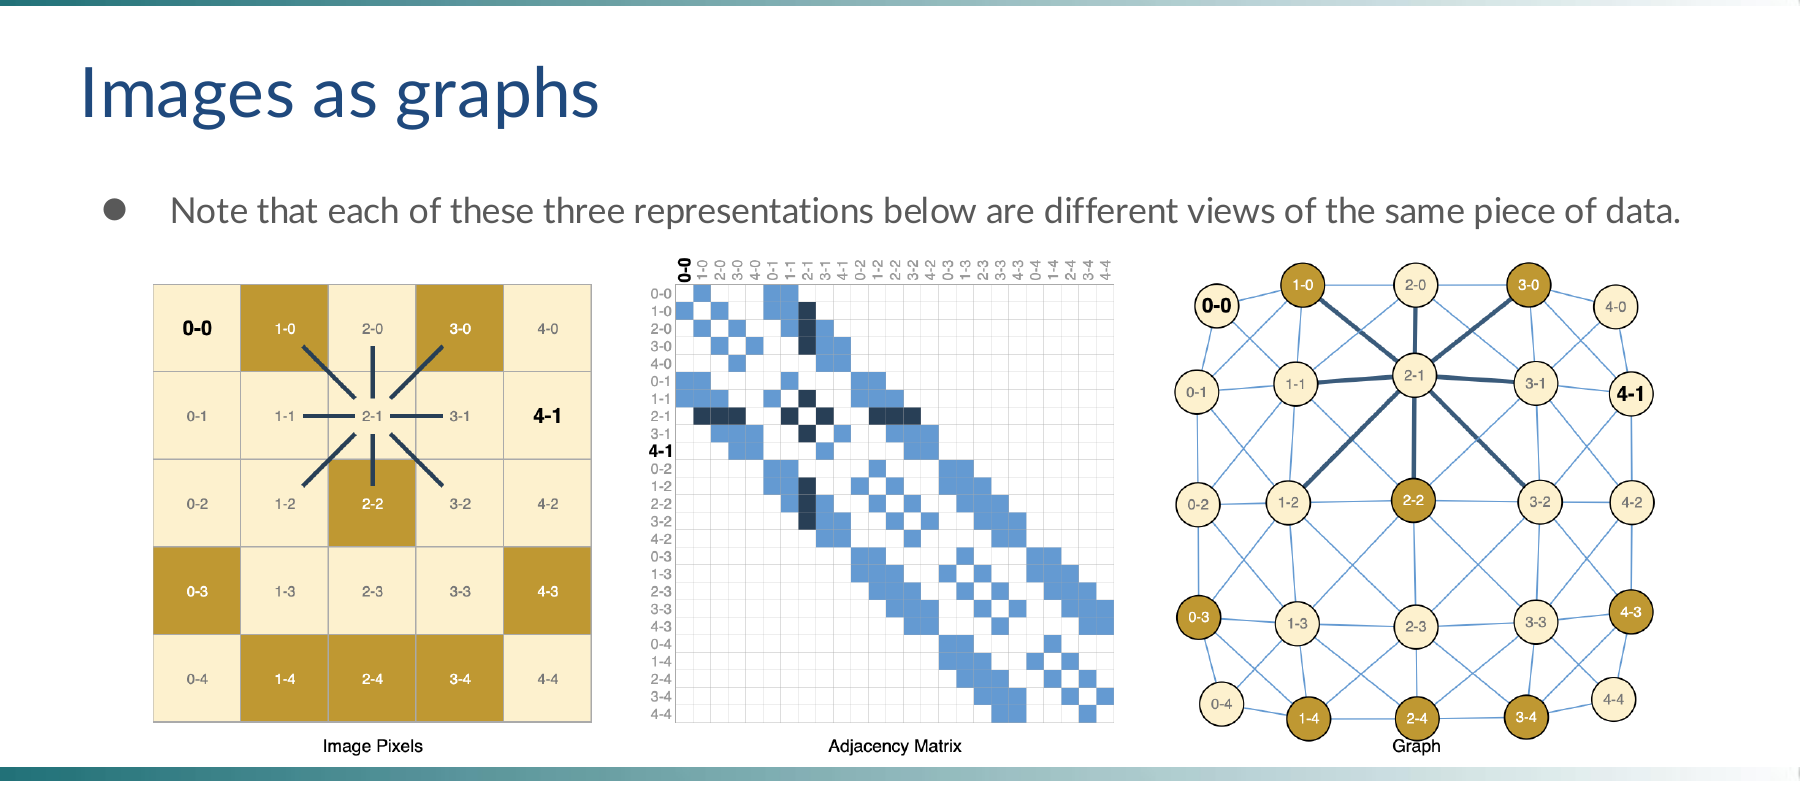
\includegraphics[width=0.92\linewidth]{figures/cf14_images_as_graphs.png}
  \caption{Tre rappresentazioni equivalenti della stessa immagine
           $5\times5$: l'immagine a pixel (sinistra), la matrice di
           adiacenza a bande (centro) e il grafo esplicito (destra).
           I nodi centrali dell'immagine hanno più connessioni rispetto
           ai nodi di bordo.}
  \label{fig:images_as_graphs}
\end{figure}

\subsection{Task su Grafi}
\label{subsec:graph-tasks}

I principali task di machine learning su grafi sono:

\begin{description}
  \item[Graph-level task] Predire una proprietà dell'intero grafo,
        ad esempio se una molecola è tossica o a cosa si lega.
        È l'analogo della classificazione di immagini con MNIST.
  \item[Node-level task] Predire l'identità o il ruolo di ciascun
        nodo. Un esempio classico è il \emph{Karate Club} di Zachary:
        classificare i membri in base all'allegiance a uno dei due
        club dopo una scissione politica. È analogo alla
        segmentazione semantica delle immagini.
  \item[Edge-level task] Predire le relazioni tra nodi (scene
        understanding) o l'esistenza di archi mancanti
        (link prediction).
  \item[Node Clustering] Raggruppare nodi simili sulla base della
        connettività.
  \item[Influence Maximization] Identificare i nodi più influenti
        in una rete.
\end{description}

\subsection{Dataset di Grafi Reali}
\label{subsec:graph-datasets}

\begin{figure}[H]
  \centering
  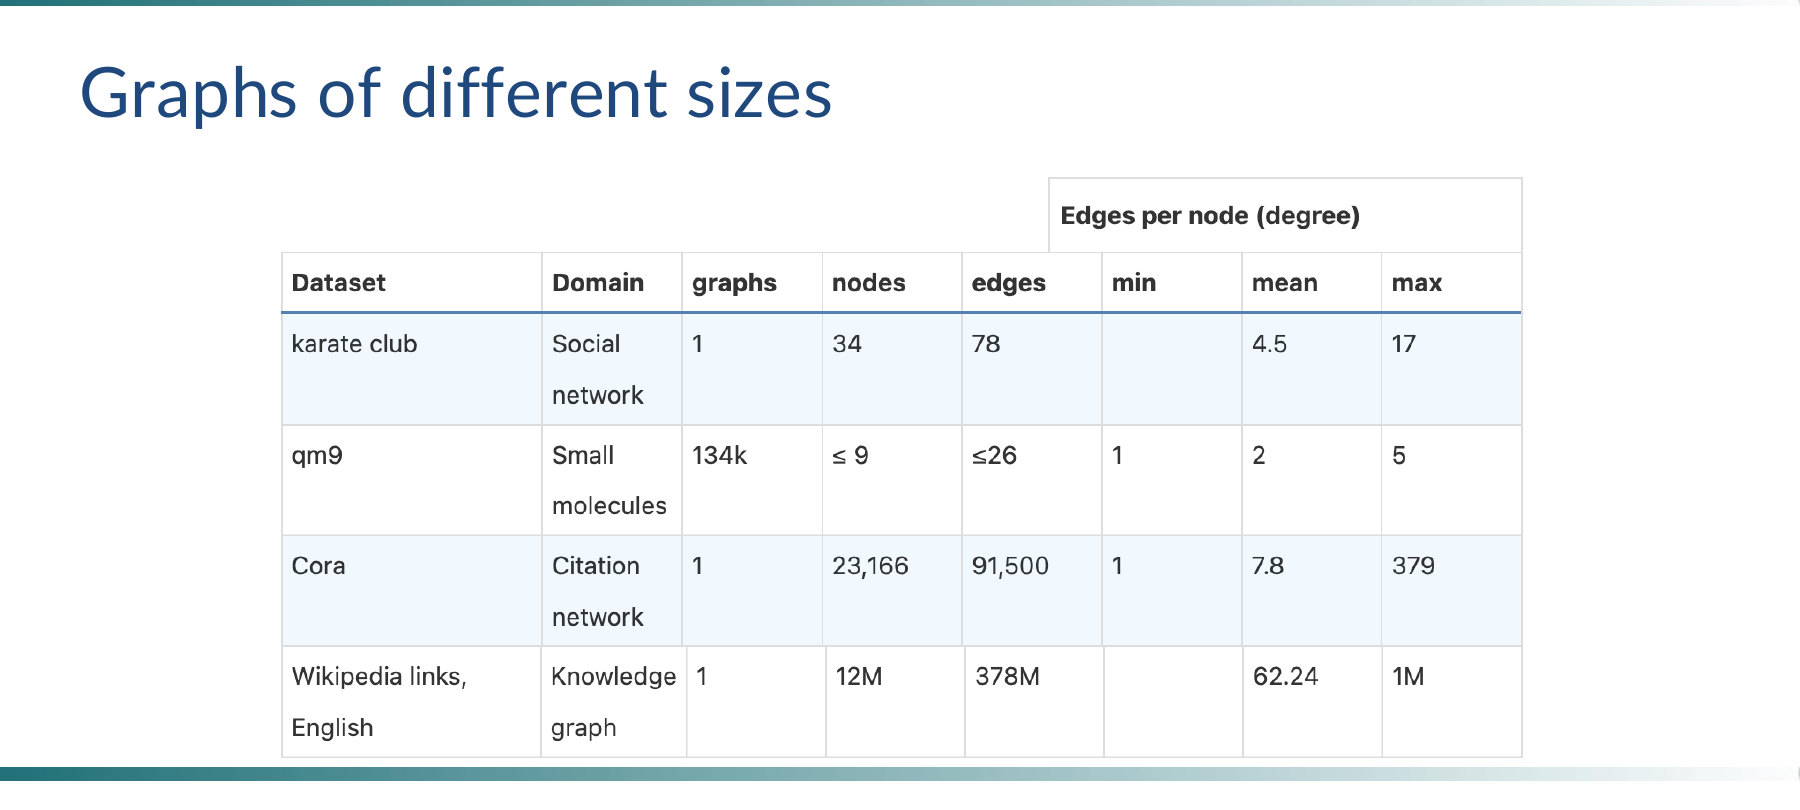
\includegraphics[width=0.82\linewidth]{figures/cf14_graph_datasets.png}
  \caption{Statistiche di dataset di grafi reali: il karate club
           (rete sociale, 34 nodi, 78 archi), QM9 (molecole piccole,
           $\leq9$ nodi, $\leq26$ archi), Cora (citation network,
           23\,166 nodi, 91\,500 archi), Wikipedia (knowledge graph,
           12M nodi, 378M archi).}
  \label{fig:graph_datasets}
\end{figure}

%------------------------------------------------------------
\section{Le Sfide del Calcolo su Grafi}
\label{sec:graph-challenges}

\subsection{Struttura Non Uniforme}
\label{subsec:irregular-structure}

I grafi sono modelli matematici estremamente flessibili, ma proprio
per questo mancano di una struttura uniforme tra istanze diverse.
Considerando la predizione di tossicità di molecole, emergono
immediatamente le seguenti difficoltà:

\begin{itemize}
  \item Le molecole possono avere numeri diversi di atomi.
  \item Gli atomi possono essere di tipo diverso.
  \item Ogni atomo può avere un numero diverso di connessioni.
  \item Le connessioni possono avere forze diverse.
\end{itemize}

\subsection{Node-Order Equivariance}
\label{subsec:equivariance}

Rappresentare un grafo come vettore richiede di fissare un ordinamento
dei nodi. Tuttavia, quando i nodi non hanno un ordine intrinseco, lo
stesso grafo può essere descritto da matrici di adiacenza diverse (una
per ogni permutazione dei nodi). Si desidera quindi che gli algoritmi
siano \textbf{node-order equivarianti}: non devono dipendere
dall'ordinamento scelto, e se i nodi vengono permutati, le
rappresentazioni risultanti devono essere permutate allo stesso modo.

\subsection{Scalabilità}
\label{subsec:scalability}

I grafi possono essere enormi (reti sociali con miliardi di utenti).
Fortunatamente, i grafi naturali sono \emph{sparsi}: il numero di archi
tende a crescere linearmente nel numero di nodi. Ciò permette di usare
metodi efficienti basati su \textbf{liste di adiacenza}, che evitano
di allocare l'intera matrice $n_{\text{nodes}}^2$.

\subsection{Rappresentazione con Liste di Adiacenza}
\label{subsec:adjacency-list}

\begin{figure}[H]
  \centering
  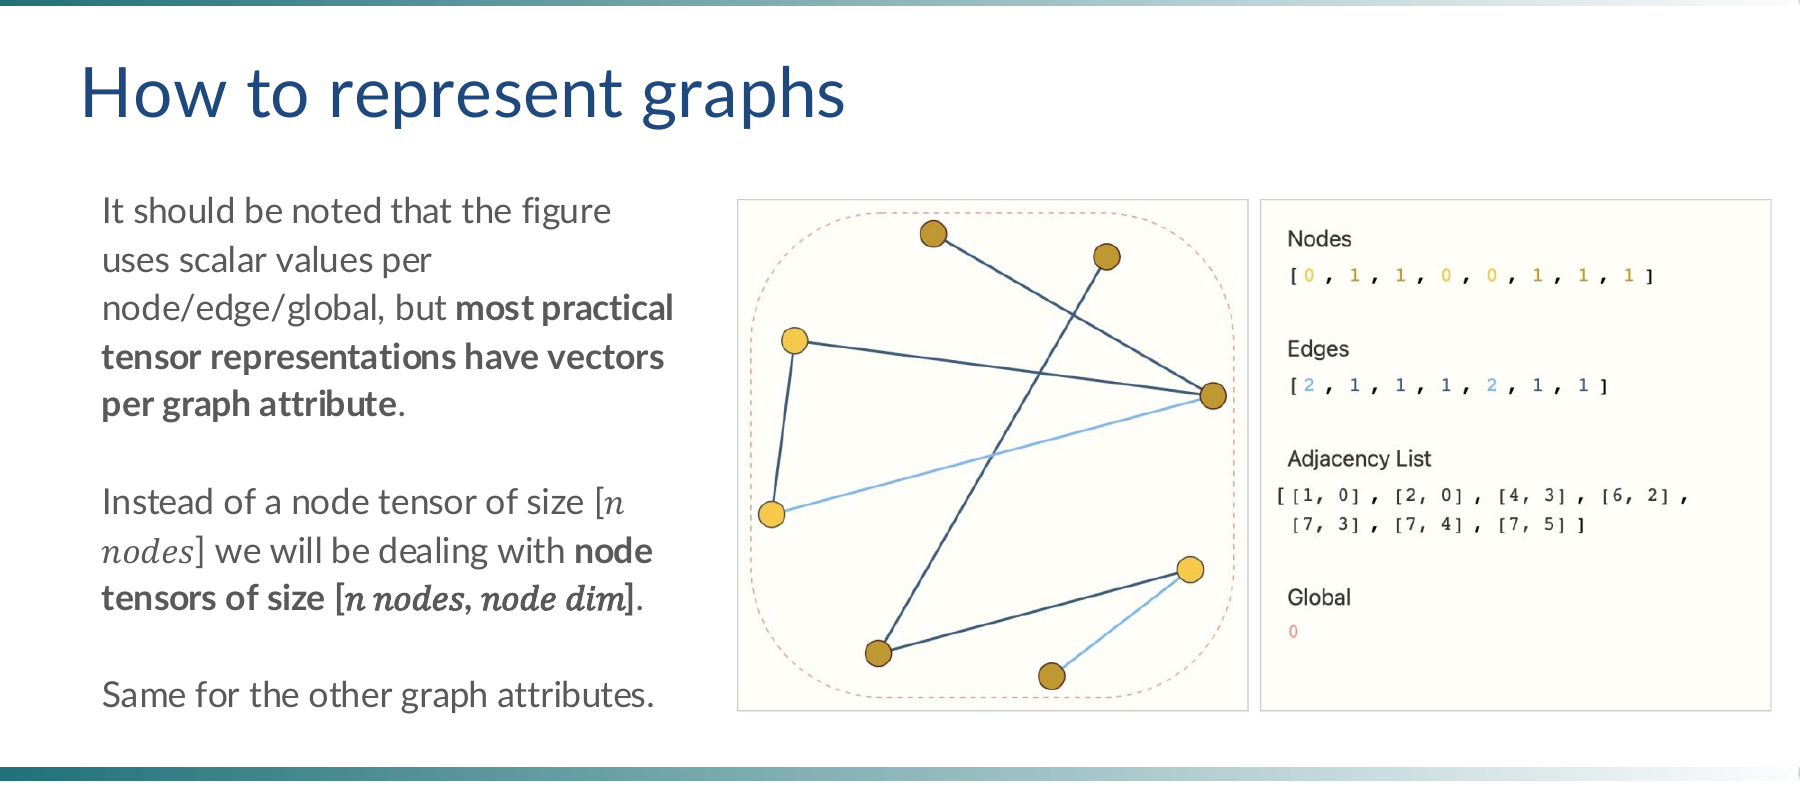
\includegraphics[width=0.88\linewidth]{figures/cf14_graph_representation.png}
  \caption{Rappresentazione di un grafo tramite lista di adiacenza.
           Ogni arco $e_k$ tra i nodi $n_i$ e $n_j$ è codificato
           come coppia $(i,j)$. In pratica ogni attributo di nodo è
           un tensore di dimensione $[n_{\text{nodes}},
           \text{node\_dim}]$ e ogni attributo di arco di dimensione
           $[n_{\text{edges}}, \text{edge\_dim}]$.}
  \label{fig:graph_representation}
\end{figure}

%------------------------------------------------------------
\section{Graph Neural Networks}
\label{sec:gnn-core}

\subsection{Definizione e Framework}
\label{subsec:gnn-def}

Una \textbf{GNN} è una trasformazione ottimizzabile su tutti gli
attributi del grafo (nodi, archi, contesto globale) che preserva le
simmetrie del grafo (invarianza alla permutazione dei nodi). Il
framework adottato è il \emph{message passing neural network}
(Gilmer et al., 2017) con la schematizzazione \emph{Graph Nets}
(Battaglia et al., 2018). Le GNN adottano un'architettura
\textbf{graph-in, graph-out}: accettano un grafo come input,
trasformano progressivamente gli embedding di nodi, archi e contesto
globale, senza modificare la connettività del grafo.

\subsection{La GNN più Semplice}
\label{subsec:simplest-gnn}

La GNN più semplice apprende nuovi embedding per tutti gli attributi
del grafo senza usare la connettività. Applica un MLP separato a
ogni componente:

\begin{itemize}
  \item Per ogni vettore nodo, l'MLP produce un nuovo vettore nodo.
  \item Per ogni arco, l'MLP produce un embedding per arco.
  \item Per il contesto globale, l'MLP produce un singolo embedding
        per l'intero grafo.
\end{itemize}

\begin{figure}[H]
  \centering
  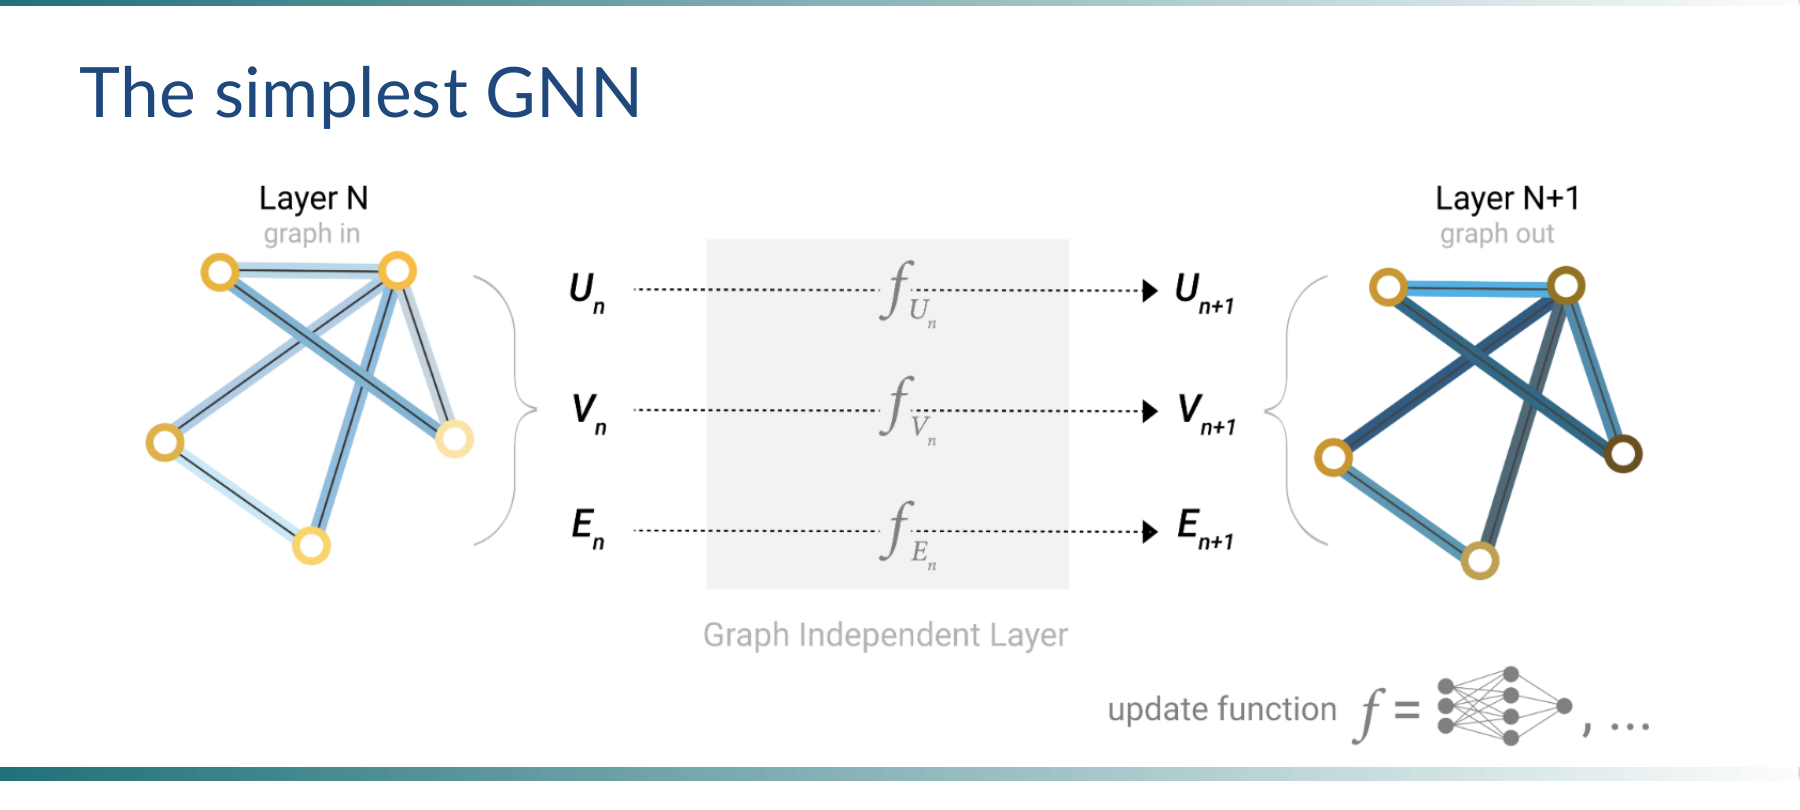
\includegraphics[width=0.88\linewidth]{figures/cf14_simplest_gnn.png}
  \caption{La GNN più semplice (Graph Independent Layer). Al layer $N$
           il grafo in ingresso ha attributi $U_n$, $V_n$, $E_n$;
           ciascuno è trasformato da una funzione di aggiornamento $f$
           (un MLP) indipendentemente dagli altri, producendo
           $U_{n+1}$, $V_{n+1}$, $E_{n+1}$ al layer $N+1$.}
  \label{fig:simplest_gnn}
\end{figure}

\subsection{Predizioni tramite Pooling}
\label{subsec:pooling}

Quando le informazioni necessarie per una predizione si trovano in un
attributo diverso da quello su cui si vuole predire, è necessario il
\textbf{pooling}. Il pooling si svolge in due passi:
\begin{enumerate}
  \item Per ogni elemento da aggregare, raccogliere tutti gli embedding
        e concatenarli in una matrice.
  \item Aggregare gli embedding raccolti, solitamente tramite somma.
\end{enumerate}

L'operazione di pooling è denotata con $\rho$, con il pedice che
indica la direzione del flusso (ad esempio $\rho_{E_n \to V_n}$
per aggregare archi verso nodi).

\subsection{Message Passing}
\label{subsec:message-passing}

Per rendere gli embedding consapevoli della connettività del grafo, si
introduce il \textbf{message passing}: i nodi (o archi) vicini si
scambiano informazioni e influenzano reciprocamente i propri embedding.
Il processo si articola in tre passi:

\begin{enumerate}
  \item Per ogni nodo, raccogliere tutti gli embedding dei nodi vicini
        (messaggi).
  \item Aggregare tutti i messaggi tramite una funzione (es.\ somma).
  \item Passare i messaggi aggregati attraverso una funzione di
        aggiornamento appresa (MLP).
\end{enumerate}

Applicando il message passing una volta si ottiene il più semplice
layer GNN con connettività. Impilando $K$ layer, un nodo incorpora
informazioni da tutti i nodi a distanza al più $K$ hop.

\begin{figure}[H]
  \centering
  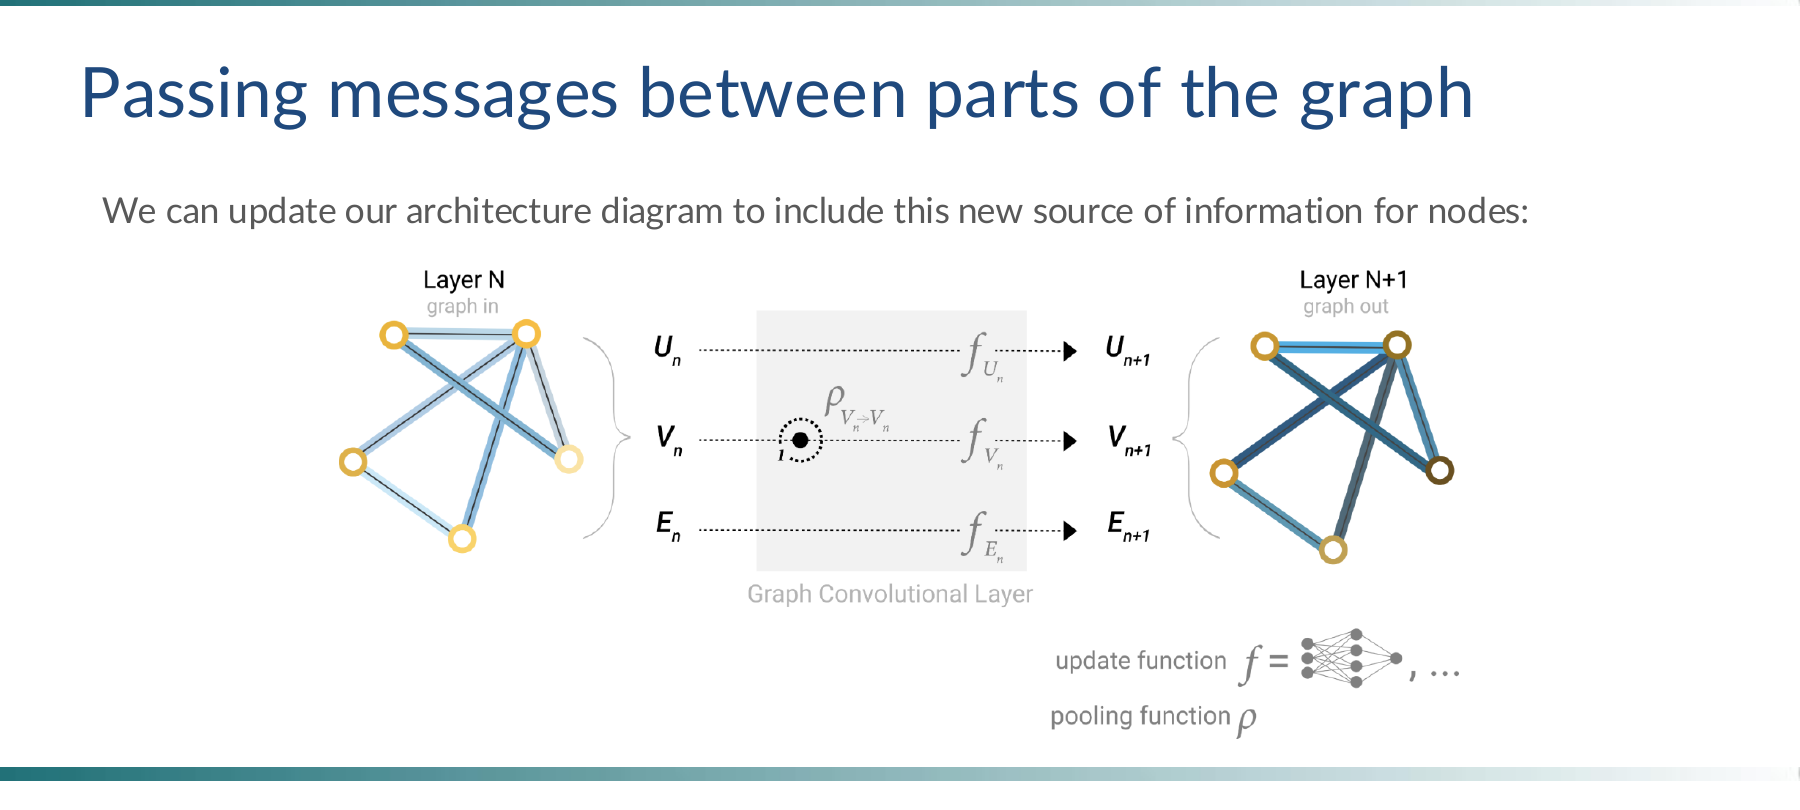
\includegraphics[width=0.92\linewidth]{figures/cf14_message_passing.png}
  \caption{Layer di Graph Convolutional con message passing. Il grafo
           al layer $N$ ha attributi $(U_n, V_n, E_n)$; la funzione
           di pooling $\rho_{V_n \to V_i}$ aggrega i vicini di ciascun
           nodo; la funzione di aggiornamento $f_{V_n}$ (MLP) produce
           i nuovi embedding $V_{n+1}$. Lo stesso avviene per $U$ e
           $E$.}
  \label{fig:message_passing}
\end{figure}

\subsection{Apprendimento di Rappresentazioni degli Archi}
\label{subsec:edge-repr}

Quando il dataset contiene solo informazioni sugli archi ma la
predizione deve essere fatta sui nodi, è possibile condividere
informazioni tra nodi e archi all'interno del layer GNN tramite
message passing. Le principali strategie di fusione sono:
concatenazione, mapping lineare dallo spazio degli archi a quello
dei nodi (o viceversa), o aggiornamento \emph{weave} che mantiene
quattro rappresentazioni aggiornate (nodo$\to$nodo, arco$\to$arco,
nodo$\to$arco, arco$\to$nodo).

\subsection{Rappresentazioni Globali}
\label{subsec:global-repr}

Un limite delle reti descritte finora è che nodi molto distanti
potrebbero non riuscire a scambiare informazioni in modo efficiente
anche con molti layer di message passing (con $K$ layer, l'informazione
si propaga al massimo $K$ hop). La soluzione adottata in Graph Nets
è il \textbf{vettore di contesto globale} $U$ (\emph{master node}),
connesso a tutti i nodi e archi della rete, che funge da canale di
comunicazione a lungo raggio.

\begin{figure}[H]
  \centering
  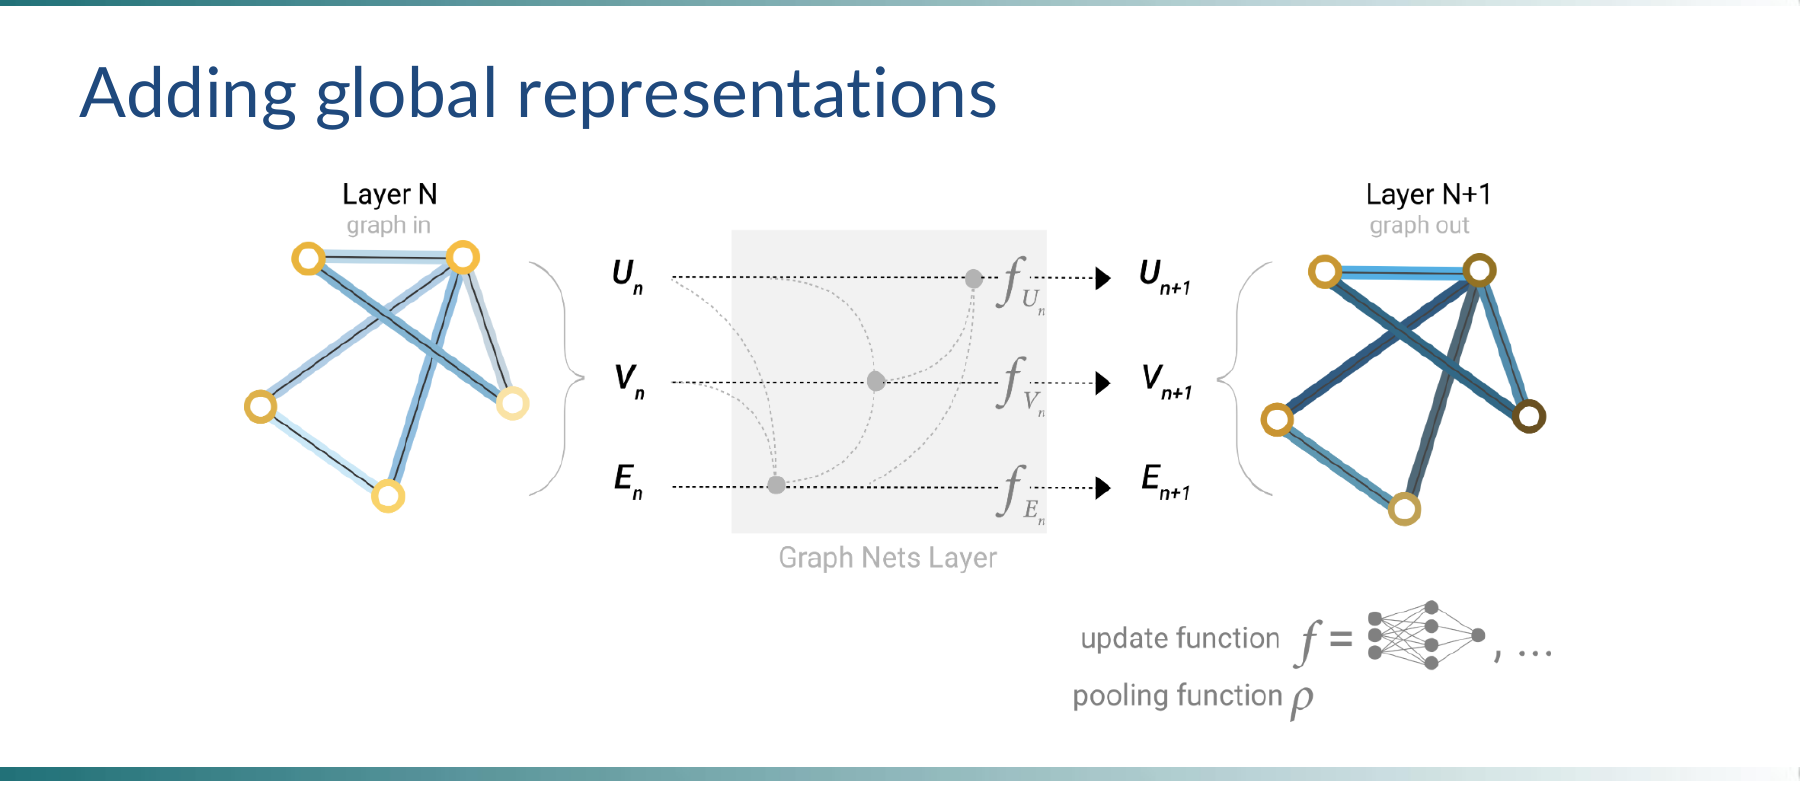
\includegraphics[width=0.92\linewidth]{figures/cf14_global_representations.png}
  \caption{Graph Nets Layer con rappresentazioni globali. Il vettore
           globale $U_n$ è connesso a tutti i nodi e archi, agendo da
           ponte per il trasferimento di informazioni a lungo raggio.
           Le funzioni di aggiornamento $f_{U_n}$, $f_{V_n}$,
           $f_{E_n}$ sono MLP condivisi.}
  \label{fig:global_repr}
\end{figure}

\subsection{Funzioni di Condizionamento}
\label{subsec:conditioning}

Con tutti gli attributi del grafo dotati di rappresentazioni apprese,
è possibile condizionare l'embedding di un nodo su tutte le sorgenti
di informazione disponibili: nodi vicini, archi connessi e
rappresentazione globale.

\begin{figure}[H]
  \centering
  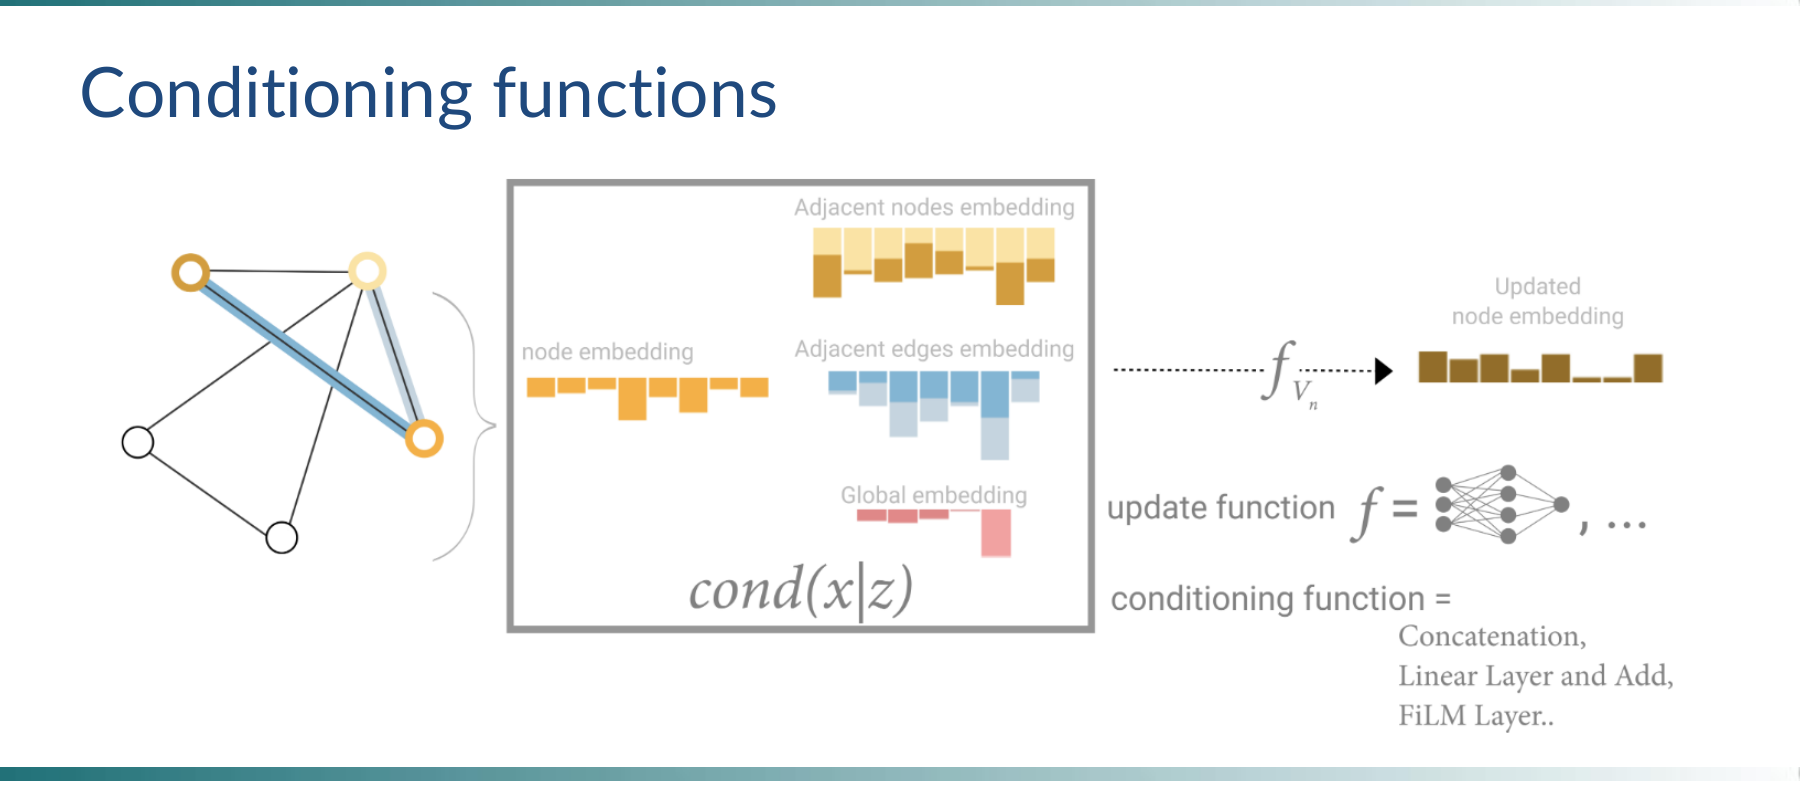
\includegraphics[width=0.88\linewidth]{figures/cf14_conditioning_functions.png}
  \caption{Funzione di condizionamento $\text{cond}(x|z)$ per un
           nodo. L'embedding del nodo viene concatenato con gli
           embedding degli archi adiacenti, dei nodi vicini e del
           vettore globale, quindi trasformato dall'update function
           $f_{V_n}$. Le opzioni di condizionamento includono
           concatenazione, layer lineare + add e FiLM layer.}
  \label{fig:conditioning}
\end{figure}

%------------------------------------------------------------
\section{GNN in a Nutshell: Formalizzazione}
\label{sec:gnn-math}

L'operazione matematica primaria in una GNN è lo schema di
\emph{message passing}, eseguito iterativamente su più layer.

\paragraph{Node Aggregation.} Per ogni nodo $i$, la funzione di
aggregazione combina le rappresentazioni dei nodi vicini $j$ e del
nodo corrente $i$:
\begin{equation}
  m_i^{(l)} = \sum_{j \in \mathcal{N}(i)}
  f^{(l)}\!\left(h_j^{(l-1)},\, h_i^{(l-1)},\, e_{ij}\right)
  \label{eq:gnn-aggregation}
\end{equation}
dove $h_i^{(l-1)}$ è la rappresentazione del nodo $i$ al layer
precedente, $e_{ij}$ è l'attributo dell'arco $(i,j)$ e $f^{(l)}$
è una funzione apprendibile.

\paragraph{Node Update.} I risultati dell'aggregazione vengono usati
per aggiornare la rappresentazione del nodo:
\begin{equation}
  h_i^{(l)} = g^{(l)}\!\left(h_i^{(l-1)},\, m_i^{(l)}\right)
  \label{eq:gnn-update}
\end{equation}
dove $g^{(l)}$ è una funzione apprendibile (tipicamente un MLP).

\paragraph{Graph-level Readout.} Una funzione di readout aggrega le
rappresentazioni dei nodi per ottenere una rappresentazione a livello
di grafo:
\begin{equation}
  h_G = \text{READOUT}\!\left(\left\{h_i^{(K)} \mid i \in V\right\}\right)
  \label{eq:gnn-readout}
\end{equation}

%------------------------------------------------------------
\section{Filtri Polinomiali e Graph Laplacian}
\label{sec:spectral}

\subsection{Il Graph Laplacian}
\label{subsec:laplacian}

Dato un grafo $G$ con $n$ nodi, sia $A$ la matrice di adiacenza
$0$-$1$ e $D$ la matrice diagonale dei gradi, dove
$D_{vv} = \sum_u A_{vu}$. Il \textbf{Graph Laplacian} è definito come:
\begin{equation}
  L = D - A
  \label{eq:laplacian}
\end{equation}

$L$ è il discreto analogo dell'operatore Laplaciano. È
\emph{positivo semidefinito} (tutti gli autovalori $\geq 0$) e
codifica la stessa informazione della matrice di adiacenza $A$:
dati $A$ o $L$, è possibile ricostruire l'altro. Il Laplacian
compare in numerosi problemi matematici su grafi: random walks,
spectral clustering, diffusione.

\begin{figure}[H]
  \centering
  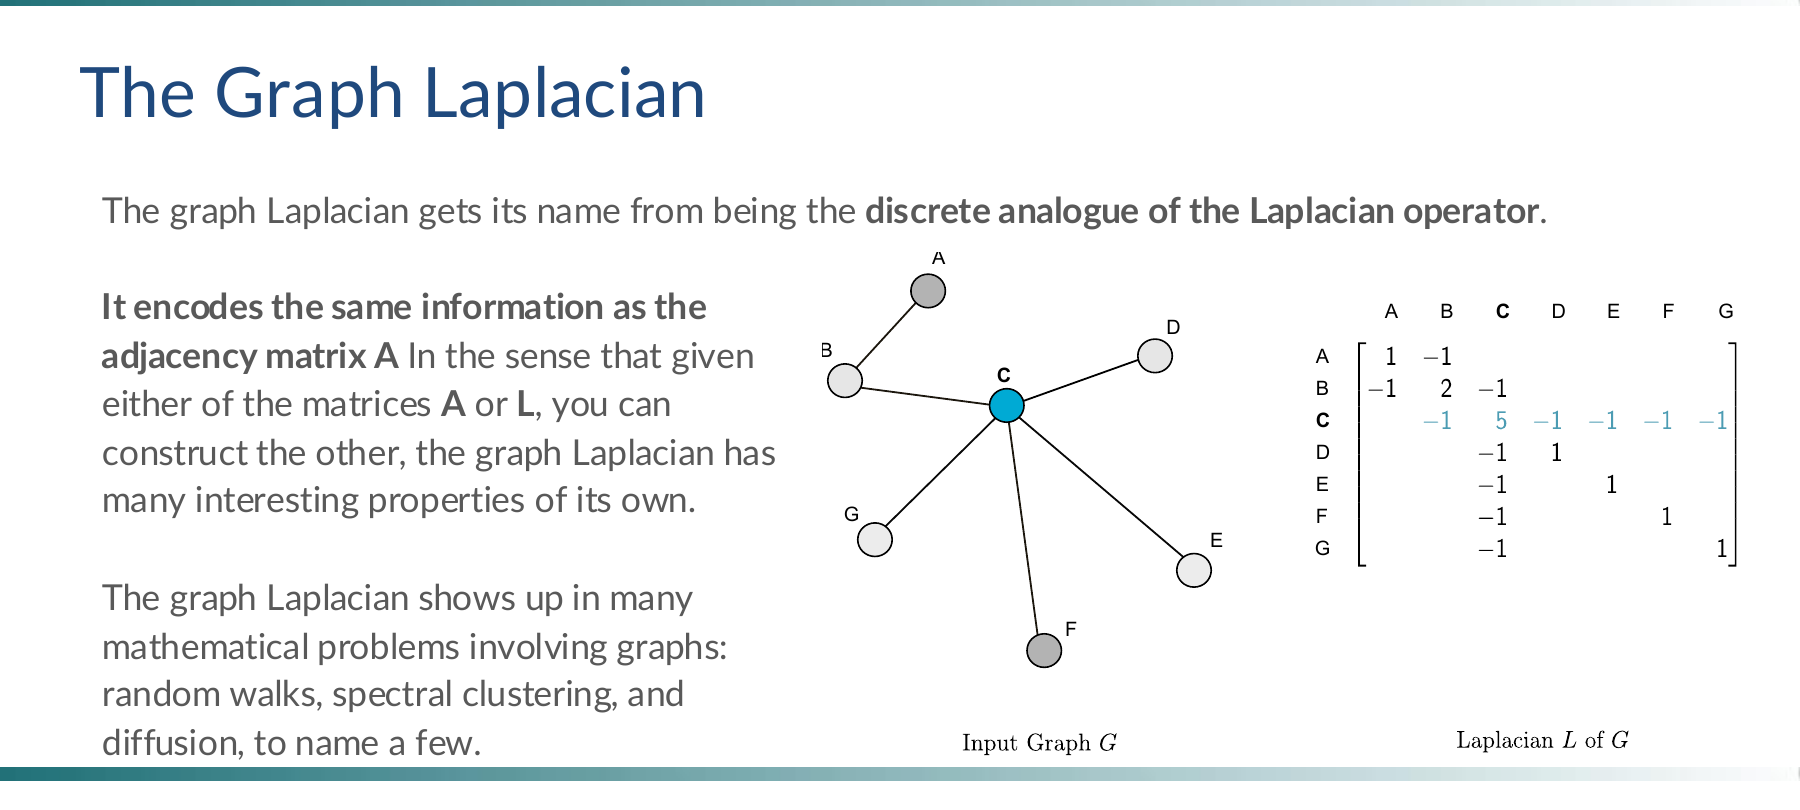
\includegraphics[width=0.88\linewidth]{figures/cf14_graph_laplacian.png}
  \caption{Un grafo $G$ con 7 nodi (sinistra) e la sua matrice
           Laplaciana $L = D - A$ (destra). Il nodo $C$, avente
           grado 5, ha $L_{CC} = 5$; gli archi incidenti in $C$
           producono $-1$ nelle posizioni corrispondenti. La riga
           highlighted (turchese) mostra la riga di $C$ nella
           matrice $L$.}
  \label{fig:graph_laplacian}
\end{figure}

\subsection{Filtri Polinomiali}
\label{subsec:poly-filters}

Si possono costruire \textbf{filtri polinomiali} del Laplacian della
forma:
\begin{equation}
  p_w(L) = \sum_{d=0}^{D} w_d\, L^d
  \label{eq:poly-filter}
\end{equation}

I coefficienti $w = [w_0, \ldots, w_D]$ sono i pesi appresi del
filtro, analogi ai pesi dei filtri nelle CNN. La convoluzione del
segnale $x \in \mathbb{R}^n$ (vettore delle feature dei nodi) con
il filtro $p_w$ è:
\begin{equation}
  x' = p_w(L)\, x
  \label{eq:poly-conv}
\end{equation}

La potenza $L^d$ ha la proprietà che $(L^d)_{vu} \neq 0$ solo se il
nodo $u$ è a distanza al più $d$ hop dal nodo $v$. Pertanto, il
filtro polinomiale di grado $d$ è \textbf{localizzato}: la
convoluzione al nodo $v$ coinvolge solo i nodi a distanza al massimo
$d$ hop. Il grado controlla la localizzazione.

\subsection{ChebNet}
\label{subsec:chebnet}

\textbf{ChebNet} (Defferrard et al., 2016) raffina i filtri
polinomiali usando i polinomi di Chebyshev di primo tipo $T_i$
applicati al Laplacian normalizzato $\tilde{L}$:
\begin{equation}
  p_w(\tilde{L}) = \sum_{i=0}^{D} w_i\, T_i(\tilde{L}),
  \qquad
  \tilde{L} = \frac{2L}{\lambda_{\max}(L)} - I
  \label{eq:chebnet}
\end{equation}

La normalizzazione garantisce che gli autovalori di $\tilde{L}$ siano
nell'intervallo $[-1, 1]$, prevenendo l'esplosione delle potenze di
$L$. I polinomi di Chebyshev assicurano stabilità numerica
nell'interpolazione. I filtri polinomiali sono node-order equivarianti
per costruzione (la somma sulle feature dei vicini non dipende
dall'ordine).

\paragraph{Embedding computation.} Impilando $K$ layer di ChebNet
con non-linearità, si ottiene una rete profonda in cui il $k$-esimo
layer ha i propri pesi appresi $w^{(k)}$:
\begin{equation}
  x^{(k)} = \sigma\!\left(p_{w^{(k)}}(\tilde{L})\, x^{(k-1)}\right)
  \label{eq:chebnet-stacked}
\end{equation}

I pesi del filtro sono condivisi tra tutti i nodi, esattamente come
il weight-sharing nelle CNN su griglia.

%------------------------------------------------------------
\section{Architetture GNN Moderne}
\label{sec:modern-gnn}

\subsection{Graph Convolutional Networks (GCN)}
\label{subsec:gcn}

Le \textbf{Graph Convolutional Networks} (Kipf \& Welling, 2017)
semplificano ChebNet limitando il filtro al primo ordine ($D=1$) e
applicando un'ulteriore normalizzazione simmetrica. La regola di
propagazione al layer $k$ è:

\begin{equation}
  h_v^{(k)} = f^{(k)}\!\left(
    W^{(k)} \cdot \frac{\sum_{u \in \mathcal{N}(v)} h_u^{(k-1)}}{|\mathcal{N}(v)|}
    + B^{(k)} \cdot h_v^{(k-1)}
  \right)
  \quad \forall\, v \in V
  \label{eq:gcn}
\end{equation}

dove $h_v^{(k)}$ è l'embedding del nodo $v$ al layer $k$,
$\mathcal{N}(v)$ è il vicinato di $v$, $W^{(k)}$ e $B^{(k)}$ sono
matrici di peso apprendibili e $f^{(k)}$ è una funzione non lineare.

\begin{figure}[H]
  \centering
  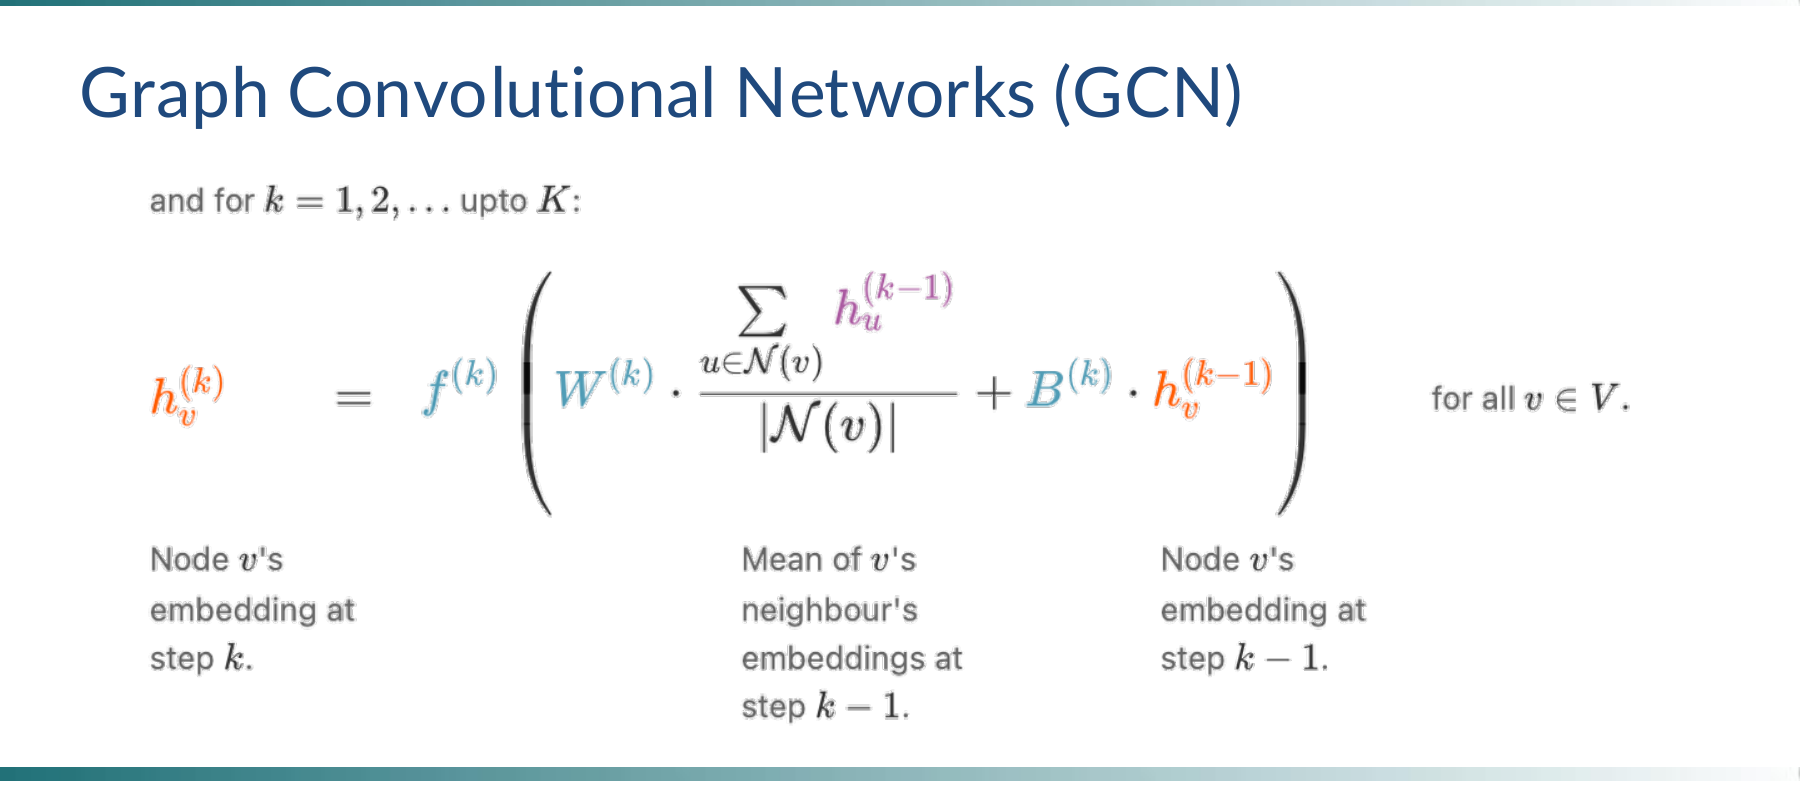
\includegraphics[width=0.88\linewidth]{figures/cf14_gcn_equation.png}
  \caption{Equazione di propagazione GCN. L'embedding
           $h_v^{(k)}$ (rosso) è una funzione apprendibile
           $f^{(k)}$ della media pesata degli embedding dei vicini
           (viola) e dell'embedding del nodo stesso al layer
           precedente (arancione). I pesi $W^{(k)}$ e $B^{(k)}$
           sono condivisi tra tutti i nodi, garantendo la scalabilità
           del modello.}
  \label{fig:gcn_equation}
\end{figure}

La normalizzazione GCN originale usa $\hat{A} = \tilde{D}^{-1/2}
\tilde{A}\, \tilde{D}^{-1/2}$ con $\tilde{A} = A + I$ (aggiunta di
auto-loop), più stabile dell'aggregazione semplice al denominatore.
La predizione finale è:
\begin{equation}
  \hat{y}_v = \text{PREDICT}\!\left(h_v^{(K)}\right)
  \label{eq:gcn-predict}
\end{equation}

\paragraph{Vantaggi GCN.} Il numero di parametri del modello
(proporzionale a $\text{node\_dim}^2 \times K$) è indipendente dalla
dimensione del grafo, garantendo buona scalabilità.

\paragraph{GCN in a nutshell.}
\begin{enumerate}
  \item \textbf{Node Aggregation}: somma pesata delle feature dei
        nodi vicini con normalizzazione per il grado:
        $\sum_{j \in \mathcal{N}(i)} \frac{h_j^{(l-1)}}{\sqrt{d_i\, d_j}}$
  \item \textbf{Node Update}: applicazione di trasformazione lineare
        e attivazione non lineare:
        $h_i^{(l)} = \sigma\!\left(W^{(l)} \cdot \text{AGG}_i\right)$
\end{enumerate}

\subsection{Graph Attention Networks (GAT)}
\label{subsec:gat}

Le \textbf{Graph Attention Networks} (Veličković et al., 2018)
sostituiscono l'aggregazione con pesi uniformi con un meccanismo
di \textbf{attenzione} appreso:

\begin{equation}
  h_v^{(k)} = f^{(k)}\!\left(
    W^{(k)} \cdot \left[
      \sum_{u \in \mathcal{N}(v)} \alpha_{vu}^{(k-1)}\, h_u^{(k-1)}
      + \alpha_{vv}^{(k-1)}\, h_v^{(k-1)}
    \right]
  \right)
  \quad \forall\, v \in V
  \label{eq:gat}
\end{equation}

\begin{figure}[H]
  \centering
  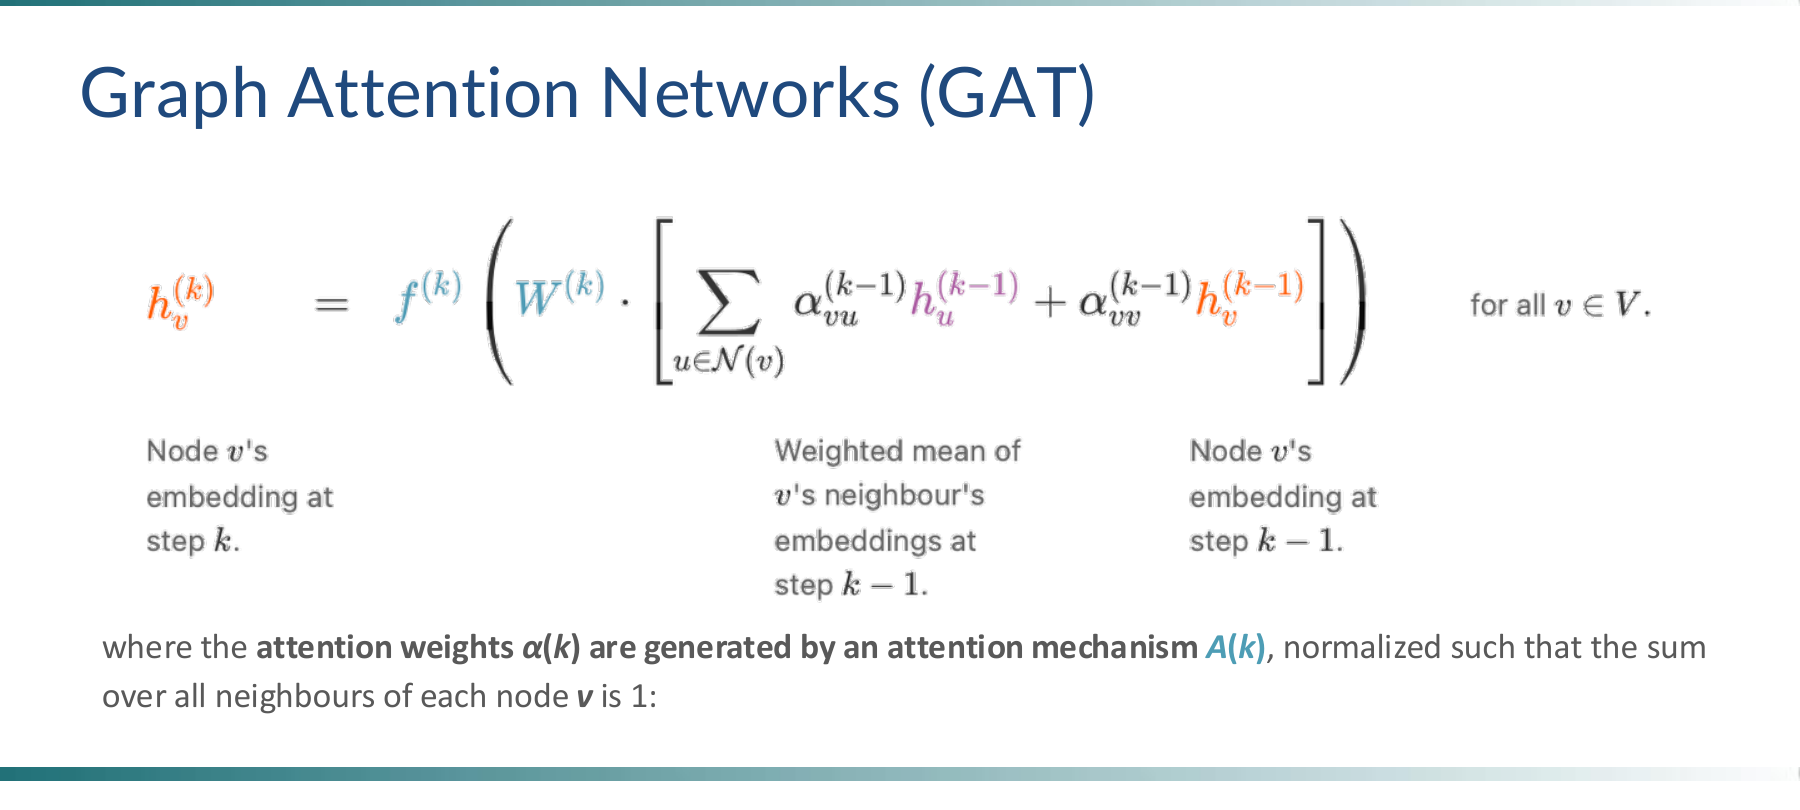
\includegraphics[width=0.88\linewidth]{figures/cf14_gat_equation.png}
  \caption{Equazione di propagazione GAT. I pesi di attenzione
           $\alpha_{vu}^{(k-1)}$ (generati dal meccanismo $A^{(k)}$,
           tipicamente un MLP) ponderano il contributo di ciascun
           vicino all'embedding del nodo. La sommatoria normalizzata
           su tutti i vicini produce la media pesata per attenzione.}
  \label{fig:gat_equation}
\end{figure}

I pesi $\alpha_{vu}^{(k)}$ sono generati da un meccanismo di
attenzione $A^{(k)}$ (spesso un piccolo MLP) e normalizzati con
softmax affinché la loro somma su tutti i vicini di $v$ sia 1:
\begin{equation}
  \sum_{u \in \mathcal{N}(v)} \alpha_{vu}^{(k)} + \alpha_{vv}^{(k)} = 1
  \label{eq:gat-norm}
\end{equation}

La variante discussa utilizza attenzione single-head; la variante
multi-head è analoga.

\subsection{GraphSAGE}
\label{subsec:graphsage}

\textbf{GraphSAGE} (Hamilton et al., 2017) introduce due innovazioni
rispetto a GCN: la scelta esplicita della funzione di aggregazione
e il \emph{neighbourhood sampling}.

La regola di aggiornamento è:
\begin{equation}
  h_v^{(k)} = f^{(k)}\!\left(
    W^{(k)} \cdot \left[h_v^{(k-1)},\, \text{AGG}\!\left(\left\{h_u^{(k-1)}\right\}_{u \in \mathcal{N}(v)}\right)\right]
  \right)
  \label{eq:graphsage}
\end{equation}

Le principali scelte per $\text{AGG}$ sono:
\begin{description}
  \item[Mean] Media degli embedding dei vicini (simile a GCN).
  \item[Max] Massimo elemento per elemento
        (\emph{dimension-wise maximum}).
  \item[LSTM] Aggregazione tramite LSTM dopo un ordinamento casuale
        dei vicini; più espressiva ma non equivariante senza
        ordinamento deterministico.
\end{description}

Il \textbf{neighbourhood sampling} campiona un sottoinsieme di
dimensione fissa del vicinato ad ogni step, indipendentemente
dalla dimensione reale del vicinato. Ciò aumenta la varianza degli
embedding ma rende GraphSAGE applicabile a grafi molto grandi.

\subsection{Graph Isomorphism Network (GIN)}
\label{subsec:gin}

Le \textbf{Graph Isomorphism Networks} (Xu et al., 2019) sono
state progettate per essere massimamente espressive, raggiungendo
il limite superiore teorico del test di isomorfismo
di Weisfeiler-Leman (WL). La regola di aggiornamento è:

\begin{equation}
  h_v^{(k)} = f^{(k)}\!\left(
    \left(1 + \epsilon^{(k)}\right) h_v^{(k-1)}
    + \sum_{u \in \mathcal{N}(v)} h_u^{(k-1)}
  \right)
  \label{eq:gin}
\end{equation}

dove $\epsilon^{(k)}$ è un parametro reale apprendibile (o fissato
a 0). L'idea chiave è che la funzione di aggregazione deve essere
\emph{iniettiva} per distinguere strutture locali diverse; la somma
(a differenza della media o del massimo) preserva questa proprietà
in spazi di feature discreti.

%------------------------------------------------------------
\section{Confronto tra Architetture GNN}
\label{sec:gnn-comparison}

\begin{table}[H]
  \centering
  \caption{Confronto tra le principali architetture GNN moderne.}
  \label{tab:gnn-comparison}
  \small
  \begin{tabularx}{\linewidth}{l X c l X}
    \toprule
    \textbf{Modello} & \textbf{Aggregazione}
      & \textbf{Att.} & \textbf{Espressività} & \textbf{Note} \\
    \midrule
    GCN       & Media normalizzata       & No           & Media       & Semplice, efficiente \\
    GAT       & Media pesata (attention) & Sì (appresa) & Alta        & Multi-head disponibile \\
    GraphSAGE & Mean / Max / LSTM        & No           & Media--Alta & Neighbourhood sampling \\
    GIN       & Somma + $\epsilon$       & No           & Massima (WL)& Teoricamente ottimale \\
    ChebNet   & Filtro polinomiale       & No           & Alta        & Base spettrale \\
    \bottomrule
  \end{tabularx}
\end{table}

\paragraph{Considerazioni pratiche.}
\begin{enumerate}
  \item \textbf{GCN} è il punto di partenza standard: semplice,
        stabile e scalabile. Preferirlo come baseline.
  \item \textbf{GAT} è preferibile quando si sospetta che i vicini
        abbiano importanza diversa; il costo computazionale è
        moderatamente superiore a GCN.
  \item \textbf{GraphSAGE} è la scelta naturale per grafi molto
        grandi (milioni di nodi) grazie al neighbourhood sampling
        e all'inductive learning.
  \item \textbf{GIN} è preferibile quando l'espressività è critica
        (es.\ task di graph isomorphism); richiede più attenzione
        alla regolarizzazione.
  \item Il numero di layer $K$ controlla il \emph{receptive field}:
        con $K$ layer ogni nodo incorpora informazioni da distanza
        al più $K$ hop. Valori tipici sono $K = 2$--$4$; aumentare
        $K$ può causare \emph{over-smoothing}.
  \item Per task \textbf{graph-level}, aggiungere una funzione di
        readout globale (sum/mean pooling o differentiable pooling).
  \item Per task \textbf{node-level} e \textbf{edge-level}, applicare
        direttamente un classificatore lineare agli embedding finali.
\end{enumerate}

%============================================================
%  Capitolo 15 – Energy-Based Models
%============================================================
\chapter{Energy-Based Models}
\label{ch:ebm}

I \textbf{modelli basati sull'energia} (\emph{Energy-Based Models}, EBM)
costituiscono un framework generale per l'apprendimento automatico che
supera i limiti delle reti neurali feed-forward classiche. Una rete
neurale tradizionale utilizza un numero finito e fisso di operazioni per
produrre un singolo output deterministico; tuttavia, molti problemi reali
richiedono o una computazione arbitrariamente complessa per derivare
l'output, oppure ammettono molteplici output compatibili con uno stesso
input (si pensi alla predizione di frame futuri in un video, o alla
traduzione automatica, dove più frasi sono ugualmente corrette). Gli EBM
affrontano questi scenari inquadrando l'inferenza come un problema di
\emph{soddisfacimento di vincoli}: si cerca l'output che minimizza una
funzione scalare chiamata \textbf{funzione energia} \citep{lecun2006tutorial,bishop2024}.

%------------------------------------------------------------
\section{Definizione e Intuizione}
\label{sec:ebm-definition}

La \textbf{funzione energia} $F(\mathbf{x}, \mathbf{y})$ è una funzione
scalare che cattura la compatibilità tra le variabili osservate
$\mathbf{x}$ (input) e le variabili da predire $\mathbf{y}$ (output):

\begin{itemize}
  \item $F(\mathbf{x}, \mathbf{y})$ assume \emph{valori bassi} quando
        $\mathbf{y}$ è compatibile con $\mathbf{x}$.
  \item $F(\mathbf{x}, \mathbf{y})$ assume \emph{valori alti} quando
        $\mathbf{y}$ è incompatibile con $\mathbf{x}$.
\end{itemize}

L'\textbf{inferenza} consiste nel trovare il valore $\hat{\mathbf{y}}$
che minimizza la funzione energia a $\mathbf{x}$ fissato:
\begin{equation}
  \hat{\mathbf{y}} = \arg\min_{\mathbf{y}}\, F(\mathbf{x}, \mathbf{y}).
  \label{eq:ebm-inference}
\end{equation}
Possono esistere più soluzioni, corrispondenti a minimi locali della
superficie energetica. È fondamentale notare che l'energia è usata
per l'inferenza, non direttamente come funzione di perdita
(\emph{loss}) durante l'addestramento.

\begin{figure}[H]
  \centering
  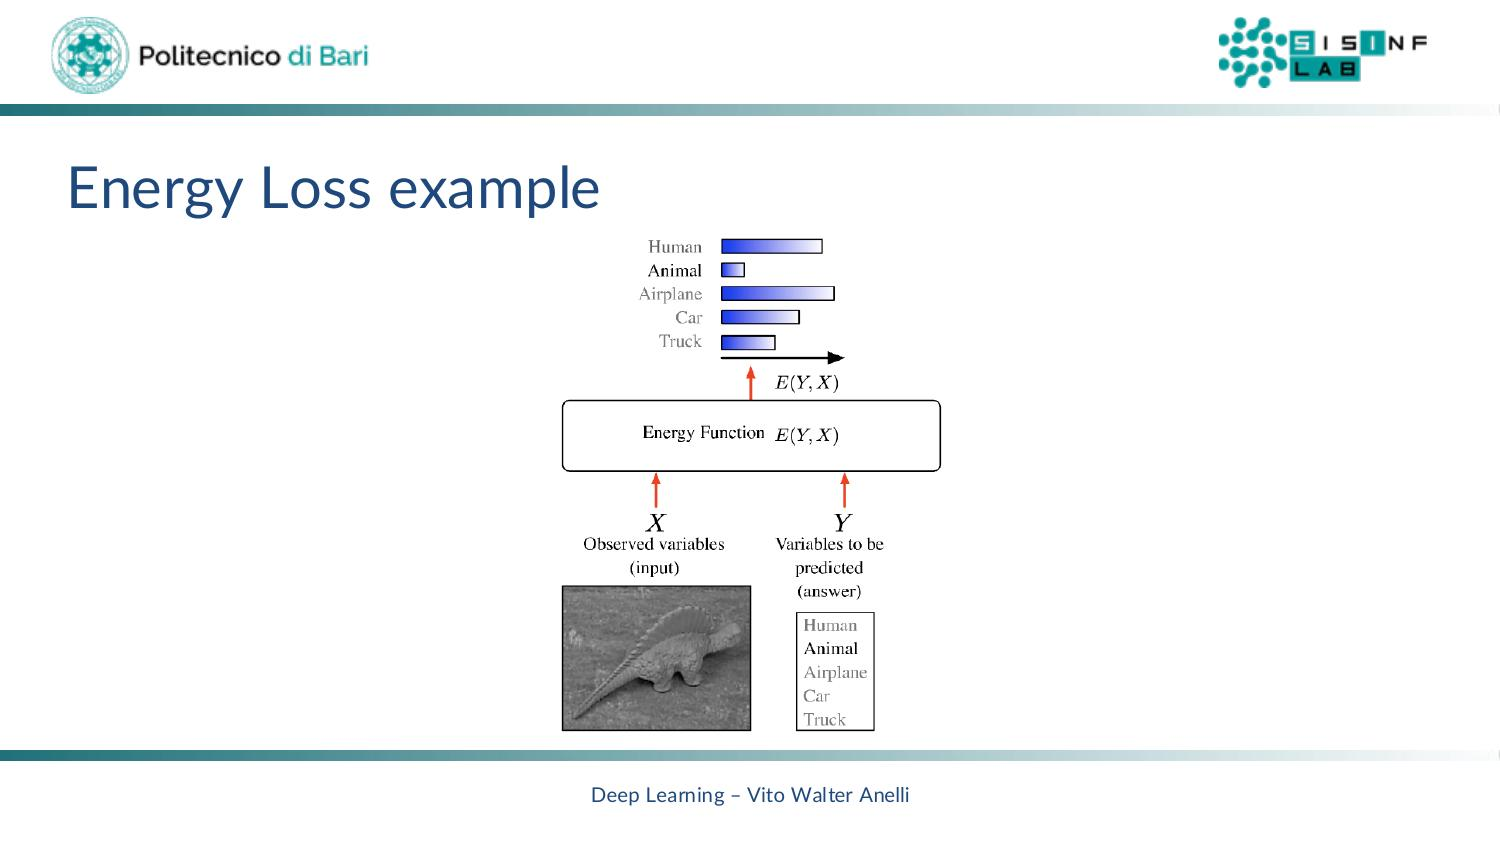
\includegraphics[width=0.85\linewidth]{figures/cf15_energy_loss_example.jpg}
  \caption{Esempio di funzione energia per un problema di classificazione.
           Dato un input $X$ (immagine di un animale) e le possibili
           etichette $Y$ \{Human, Animal, Airplane, Car, Truck\}, la
           funzione energia $E(Y,X)$ restituisce uno scalare per ogni coppia:
           un valore basso indica alta compatibilità tra $X$ e $Y$.}
  \label{fig:ebm-energy-loss-example}
\end{figure}

\subsection{Confronto con i Modelli Feed-Forward}
\label{subsec:ebm-vs-ff}

Un modello \textbf{feed-forward} è una funzione esplicita $\mathbf{y} =
G(\mathbf{x})$: ad ogni input corrisponde un unico output deterministico.
Un \textbf{EBM} è invece una funzione implicita che cattura la
dipendenza tra $\mathbf{x}$ e $\mathbf{y}$ tramite $F(\mathbf{x},
\mathbf{y})$. La differenza cruciale è che più valori di $\mathbf{y}$
possono essere compatibili con un singolo $\mathbf{x}$, corrispondendo
a minimi distinti della superficie energetica.

Perché la funzione $F$ sia utilizzabile con algoritmi di inferenza basati
su gradiente, essa deve essere \emph{liscia} e \emph{differenziabile}
rispetto a $\mathbf{y}$ (quando $\mathbf{y}$ è continuo). La superficie
energia deve presentare bassa energia in prossimità dei punti del dataset
e alta energia altrove.

\begin{figure}[H]
  \centering
  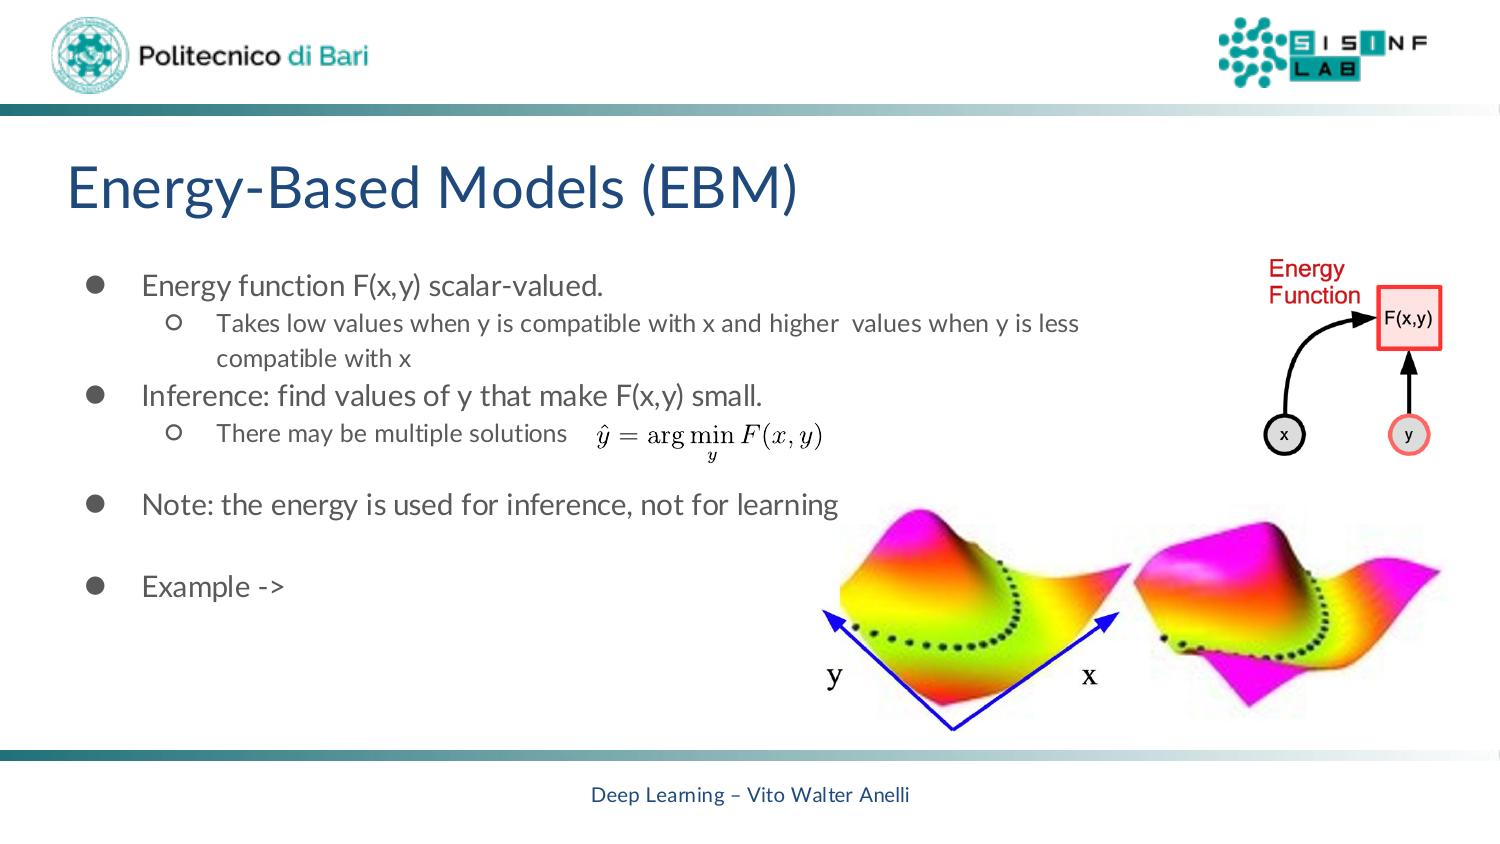
\includegraphics[width=0.85\linewidth]{figures/cf15_ebm_inference.jpg}
  \caption{Superficie energia $F(x,y)$ in funzione delle variabili $x$
           e $y$. La curva tratteggiata indica i punti del training set:
           la rete apprende a collocare i minimi della superficie in
           corrispondenza dei dati osservati. L'inferenza corrisponde a
           discendere il gradiente lungo la dimensione $y$.}
  \label{fig:ebm-inference}
\end{figure}

\subsection{Superfici Energetiche: Buon e Cattivo Addestramento}
\label{subsec:ebm-surfaces}

Un addestramento corretto modella la superficie energetica in modo che
presenti valli nette in prossimità dei dati di training e colline altrove.
Al contrario, un addestramento difettoso può portare alla cosiddetta
\textbf{soluzione collassata}: il modello ignora l'input e produce output
identici, generando una superficie piatta con energia prossima a zero
ovunque. Questo comportamento degenere è il principale rischio dei metodi
privi di un meccanismo esplicito di separazione delle regioni a bassa
energia.

\begin{figure}[H]
  \centering
  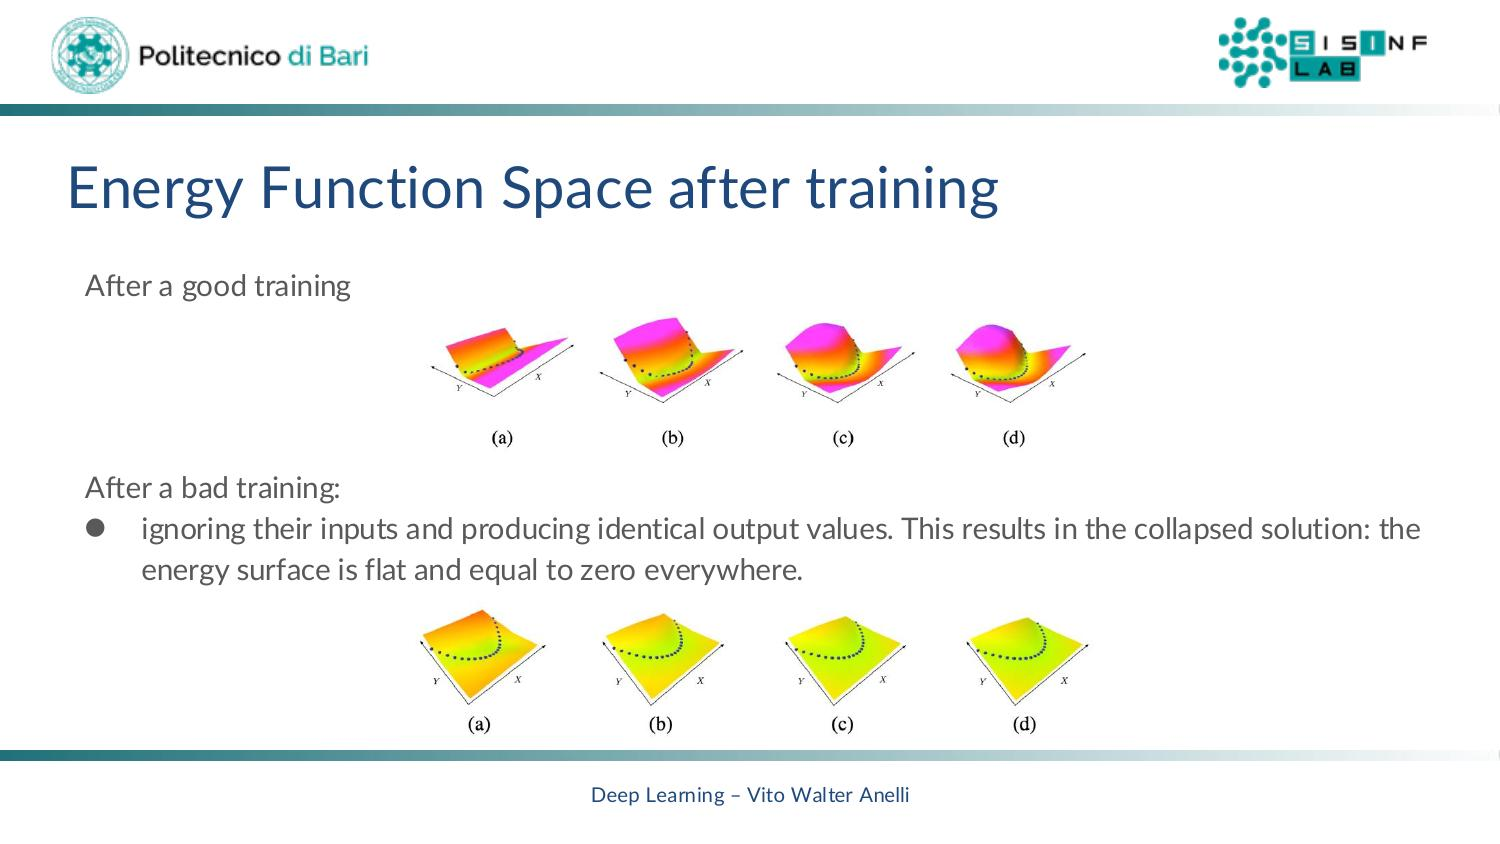
\includegraphics[width=0.88\linewidth]{figures/cf15_energy_surface_training.jpg}
  \caption{Confronto tra superfici energia dopo un buon addestramento
           (riga superiore) e un cattivo addestramento (riga inferiore).
           Nel caso degenere la superficie è piatta (energia costante),
           impedendo qualsiasi discriminazione tra output compatibili e
           incompatibili.}
  \label{fig:ebm-surfaces}
\end{figure}

%------------------------------------------------------------
\section{Architetture EBM per la Predizione Multimodale}
\label{sec:ebm-architectures}

Per gestire distribuzioni multimodali sull'output esistono due famiglie
principali di architetture: i \textbf{joint embedding architectures} e
i \textbf{latent variable models}.

\subsection{Joint Embedding}
\label{subsec:joint-embedding}

Nell'architettura a \textbf{joint embedding}, due rami encoder ($\text{Pred}(x)$
e $\text{Pred}(y)$) proiettano input e output nello stesso spazio delle
feature, producendo le rappresentazioni $\mathbf{h}$ e $\mathbf{h}'$.
La funzione energia è definita come una misura di distanza in questo spazio:
\begin{equation}
  F(\mathbf{x}, \mathbf{y}) = C\bigl(\mathbf{h},\, \mathbf{h}'\bigr),
\end{equation}
dove $C(\cdot, \cdot)$ è tipicamente la distanza euclidea o coseno.
Le multiple predizioni compatibili sono ottenute tramite invarianza alle
features piuttosto che tramite ricostruzione a livello di pixel.

Vantaggi principali:
\begin{itemize}
  \item Nessuna ricostruzione pixel-level, computazionalmente onerosa.
  \item Naturalmente invariante a distorsioni semanticamente irrilevanti
        (illuminazione, prospettiva, occlusioni parziali).
\end{itemize}

Esempi di successo per il riconoscimento di immagini includono
DeepFace~\citep{taigman2014deepface}, PIRL, MoCo e SimCLR.

\subsection{Modelli a Variabili Latenti}
\label{subsec:latent-variable-ebm}

Nei \textbf{modelli a variabili latenti} (LV-EBM), una variabile latente
$\mathbf{z}$ parametrizza l'insieme delle predizioni compatibili con
l'input. Idealmente, $\mathbf{z}$ cattura fattori esplicativi
\emph{indipendenti} della variabilità dell'output. L'architettura è
composta da:

\begin{description}
  \item[$\text{Pred}(x)$] Encoder che produce la rappresentazione
        $\mathbf{h}$ a partire dall'osservazione $\mathbf{x}$.
  \item[$\text{Dec}(\mathbf{z}, \mathbf{h})$] Decoder che genera la
        predizione $\bar{\mathbf{y}}$ combinando $\mathbf{h}$ con la
        variabile latente $\mathbf{z}$.
\end{description}

È critico che la \textbf{capacità informativa} di $\mathbf{z}$ sia
limitata: se $\mathbf{z}$ può memorizzare tutta l'informazione
sull'output, il modello potrebbe ricostruire perfettamente qualsiasi
$\mathbf{y}$ indipendentemente da $\mathbf{x}$, collassando sulla
soluzione banale con superficie piatta.

\paragraph{Esempi applicativi.}
Le variabili latenti sono particolarmente utili quando l'inferenza richiede
informazione ausiliaria non osservata. Per esempio, riconoscere una parola
manoscritta è facilitato dalla conoscenza implicita della posizione dei
caratteri; per il riconoscimento del parlato, conoscere la posizione dei
fonemi e delle parole nell'audio semplifica enormemente il task.

\subsection{LV-EBM Condizionale con Regolarizzazione}
\label{subsec:conditional-lv-ebm}

Per evitare la soluzione collassata, il modello condizionale adotta un
\textbf{regolarizzatore} $R(\mathbf{z})$ che penalizza la capacità di
$\mathbf{z}$. La funzione energia diventa:
\begin{equation}
  E(\mathbf{x}, \mathbf{y}, \mathbf{z})
  = C\!\bigl(\mathbf{y},\; \text{Dec}(\text{Pred}(\mathbf{x}),\, \mathbf{z})\bigr)
  + \lambda\, R(\mathbf{z}).
  \label{eq:conditional-lv-ebm}
\end{equation}

Esempi di regolarizzatori efficaci:
\begin{itemize}
  \item \textbf{Dimensione effettiva} \citep{li2020rethinking}: penalizza
        il rango effettivo della rappresentazione latente.
  \item \textbf{Quantizzazione/discretizzazione}: limita $\mathbf{z}$ a
        un insieme discreto di valori (come nei VQ-VAE).
  \item \textbf{Norma $\ell_0$}: minimizza il numero di componenti non nulle
        di $\mathbf{z}$.
  \item \textbf{Norma $\ell_1$} con normalizzazione del decoder.
  \item \textbf{Inibizione laterale}: promuove la competizione tra unità
        latenti.
  \item \textbf{Aggiunta di rumore} con vincolo sulla norma $\ell_2$
        di $\mathbf{z}$ (come nei VAE~\citep{kingma2013vae}).
\end{itemize}

%------------------------------------------------------------
\section{Addestramento degli EBM}
\label{sec:ebm-training}

L'obiettivo dell'addestramento è plasmare la funzione
$F_\theta(\mathbf{x},\mathbf{y})$, parametrizzata da $\theta$, in modo
che:
\begin{equation}
  F_\theta\!\bigl(\mathbf{x}^{(i)}, \mathbf{y}^{(i)}\bigr)
  <
  F_\theta\!\bigl(\mathbf{x}^{(i)}, \mathbf{y}\bigr)
  \quad \forall\, \mathbf{y} \neq \mathbf{y}^{(i)},
\end{equation}
mantenendo al contempo $F$ \emph{liscia}. I metodi di apprendimento si
dividono in due grandi categorie.

\begin{figure}[H]
  \centering
  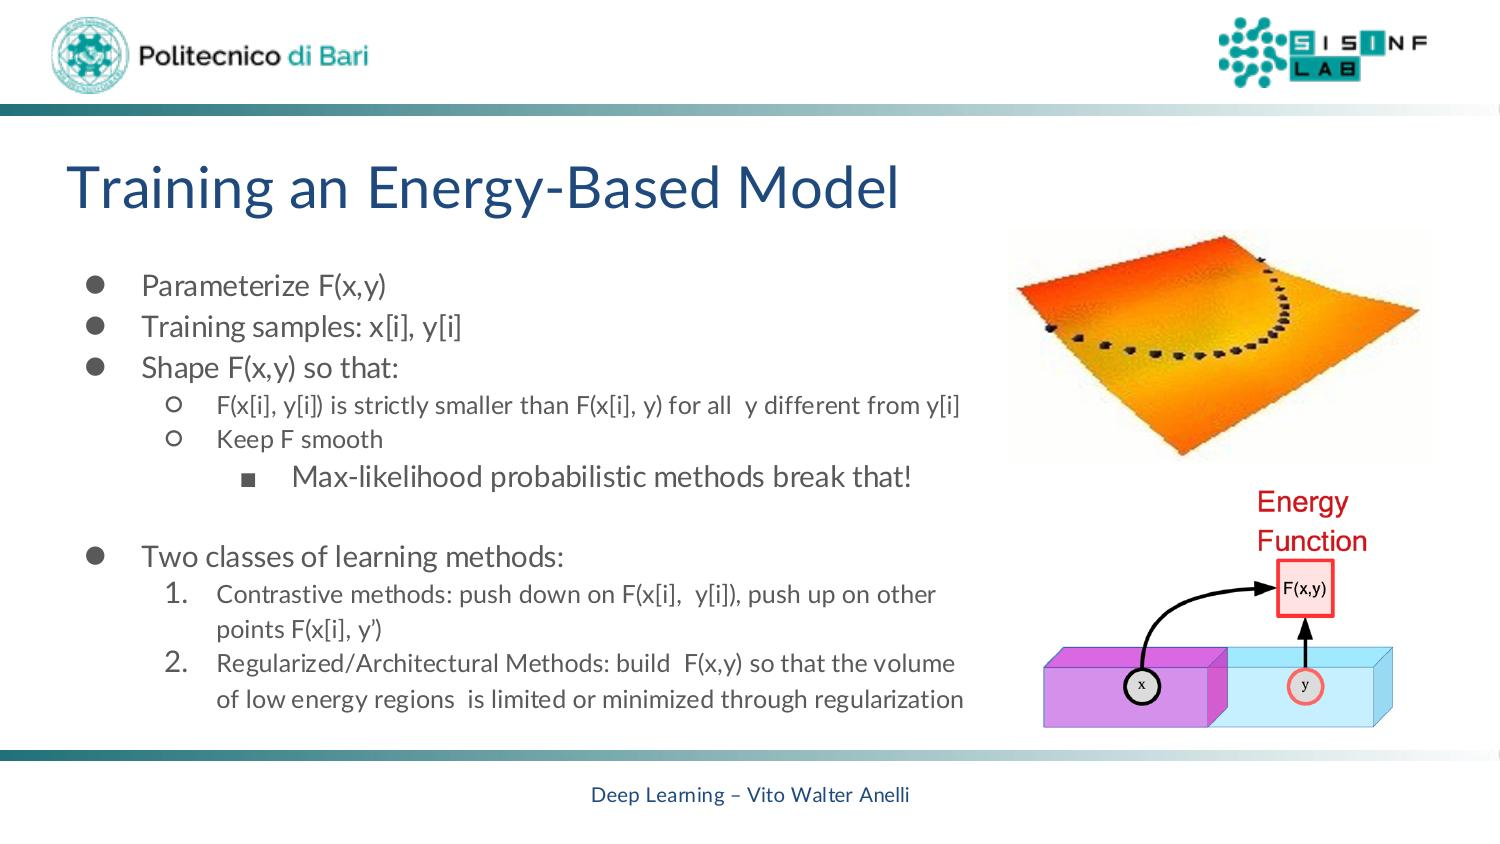
\includegraphics[width=0.75\linewidth]{figures/cf15_training_ebm.jpg}
  \caption{Configurazione per l'addestramento di un EBM. La funzione
           energia $F(\mathbf{x},\mathbf{y})$ viene parametrizzata e
           addestrata a collocare i minimi in corrispondenza dei
           campioni del training set.}
  \label{fig:ebm-training}
\end{figure}

\subsection{Metodi Contrastivi}
\label{subsec:contrastive-methods}

I \textbf{metodi contrastivi} operano con una strategia \emph{push-down /
push-up}: abbassano l'energia sui punti del training set
$(\mathbf{x}^{(i)}, \mathbf{y}^{(i)})$ e la alzano su punti alternativi
$(\mathbf{x}^{(i)}, \mathbf{y}')$ denominati \emph{campioni negativi}
o \emph{contrastivi}.

\begin{figure}[H]
  \centering
  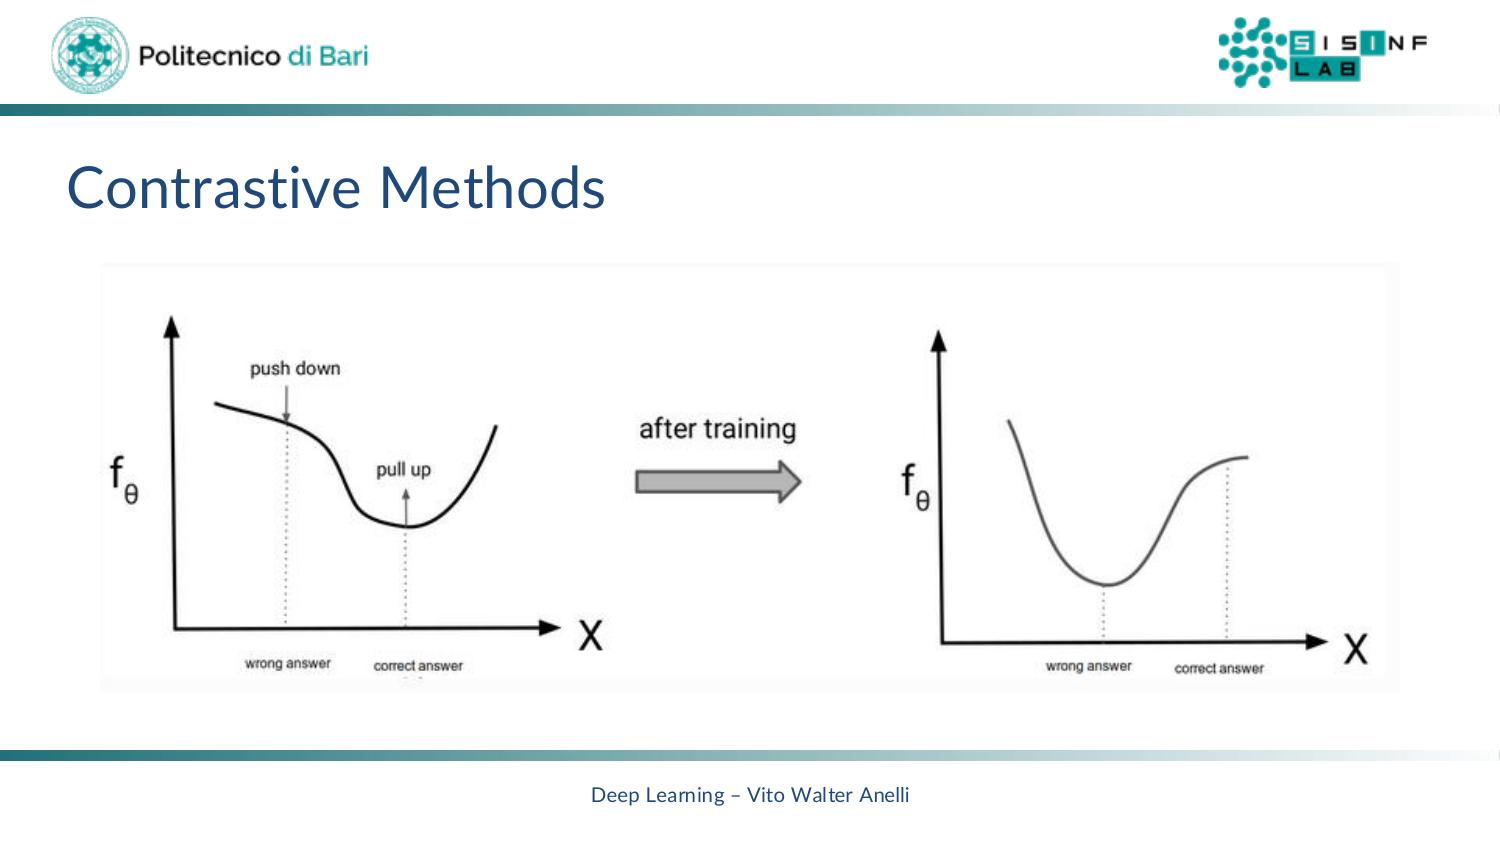
\includegraphics[width=0.80\linewidth]{figures/cf15_contrastive_push_down.jpg}
  \caption{Dinamica dei metodi contrastivi. A sinistra: lo stato iniziale
           prima dell'addestramento con frecce che indicano le direzioni
           di push-down (campione corretto) e push-up (campione errato).
           A destra: la superficie energia dopo l'addestramento, con il
           minimo ben collocato in corrispondenza dell'output corretto.}
  \label{fig:ebm-contrastive-pushdown}
\end{figure}

\paragraph{Interpretazione probabilistica.}
L'energia può essere interpretata come log-densità non normalizzata
(negativa) tramite la \textbf{distribuzione di Gibbs}:
\begin{equation}
  P(\mathbf{y} \mid \mathbf{x}) =
  \frac{\exp\!\bigl[-\beta F(\mathbf{x}, \mathbf{y})\bigr]}
       {\displaystyle\int_{\mathbf{y}'} \exp\!\bigl[-\beta F(\mathbf{x}, \mathbf{y}')\bigr]\, \mathrm{d}\mathbf{y}'},
  \label{eq:gibbs}
\end{equation}
dove $\beta > 0$ è un parametro analogo alla temperatura inversa. Il
denominatore è la \textbf{funzione di partizione} $Z(\mathbf{x})$, spesso
intrattabile per spazi continui ad alta dimensione: questo è il motivo
principale per cui si preferisce evitare l'approccio probabilistico quando
non strettamente necessario.

\paragraph{Massima verosimiglianza.}
Massimizzare $P(\mathbf{y}^{(i)} \mid \mathbf{x}^{(i)})$ equivale a
minimizzare la \emph{negative log-likelihood} (NLL):
\begin{equation}
  \mathcal{L}(\mathbf{y},\mathbf{w})
  = E(\mathbf{y}, \mathbf{w})
  + \frac{1}{\beta}\log\!\int_{\mathbf{y}'} e^{-\beta E(\mathbf{y}',\mathbf{w})},
  \label{eq:nll-loss}
\end{equation}
dove il primo termine va minimizzato (abbassare l'energia sul campione
corretto) e il secondo va massimizzato (alzare l'energia ovunque altrove).

\paragraph{Problema con la massima verosimiglianza.}
La NLL tende a creare un canyon infinitamente profondo e stretto attorno
alla varietà dei dati: vuole massimizzare la differenza di energia tra
i punti del dataset e quelli appena fuori di esso. Questo rende la
superficie non liscia e incompatibile con l'inferenza basata su gradiente.
È pertanto necessario regolarizzare la funzione di perdita (ad esempio con
la distanza di Wasserstein nelle WGAN) per recuperare la proprietà di
smoothness.

\begin{figure}[H]
  \centering
  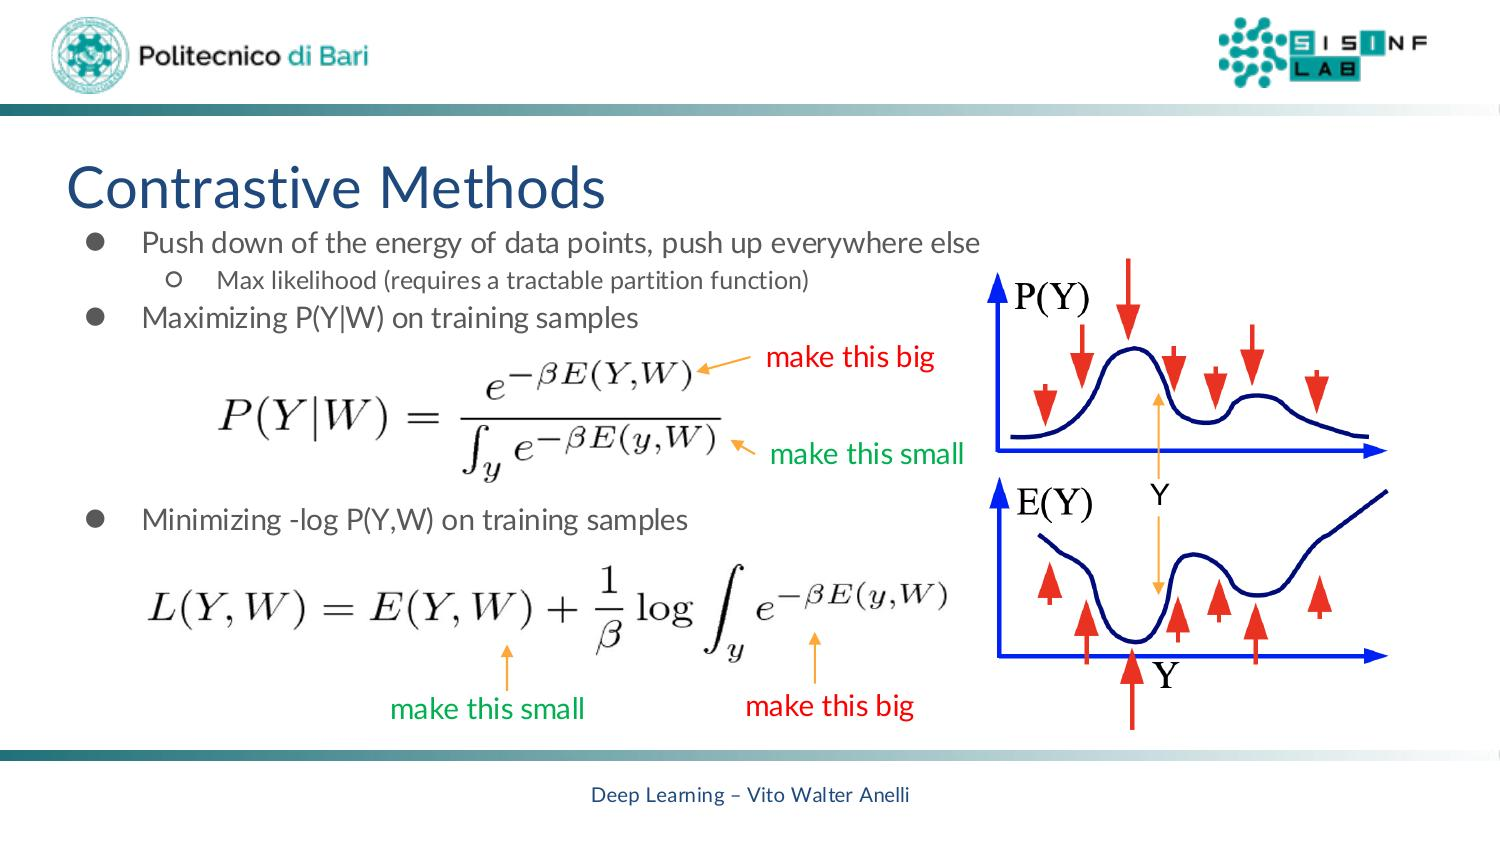
\includegraphics[width=0.85\linewidth]{figures/cf15_contrastive_methods.jpg}
  \caption{Metodi contrastivi in pratica: la probabilità $P(Y|W)$ viene
           massimizzata (riga superiore) portando a un abbassamento
           dell'energia sui campioni corretti e a un innalzamento
           ovunque altrove (riga inferiore).}
  \label{fig:ebm-contrastive}
\end{figure}

\subsection{Addestramento con MCMC}
\label{subsec:mcmc-training}

L'algoritmo pratico per l'addestramento contrastivo, proposto in
\citet{du2019implicit}, sfrutta un buffer di campioni e la
\emph{Langevin dynamics} (una forma di MCMC) per generare campioni negativi:

\begin{enumerate}
  \item Campionare un esempio reale $\mathbf{x}^+_i \sim p_\mathcal{D}$.
  \item Estrarre un campione iniziale dal buffer $B$ con probabilità 95\%,
        o da $\mathcal{U}(-1,1)$ con probabilità 5\%.
  \item Per $k = 1,\ldots,K$ passi, aggiornare il campione con la
        \textbf{Langevin dynamics}:
        \begin{equation}
          \tilde{\mathbf{x}}^k \leftarrow \tilde{\mathbf{x}}^{k-1}
          - \eta\, \nabla_{\mathbf{x}} E_\theta(\tilde{\mathbf{x}}^{k-1})
          + \omega,
          \quad \omega \sim \mathcal{N}(0,\sigma),
        \end{equation}
        ottenendo il campione negativo $\mathbf{x}^- = \tilde{\mathbf{x}}^K$.
  \item Calcolare la \textbf{contrastive divergence loss}:
        \begin{equation}
          \mathcal{L}_{CD} = \frac{1}{N}\sum_i
          E_\theta(\mathbf{x}^+_i) - E_\theta(\mathbf{x}^-_i),
        \end{equation}
        e la \textbf{regularization loss}:
        \begin{equation}
          \mathcal{L}_{RG} = \frac{1}{N}\sum_i
          \bigl[E_\theta(\mathbf{x}^+_i)\bigr]^2
          + \bigl[E_\theta(\mathbf{x}^-_i)\bigr]^2.
        \end{equation}
  \item Aggiornare i parametri con SGD/Adam su
        $\nabla_\theta(\mathcal{L}_{CD} + \alpha\,\mathcal{L}_{RG})$.
  \item Aggiungere $\mathbf{x}^-$ al buffer $B$.
\end{enumerate}

\subsection{Metodi Regolarizzati e Architetturali}
\label{subsec:regularized-methods}

I \textbf{metodi regolarizzati} non richiedono campioni negativi espliciti:
costruiscono $F(\mathbf{x},\mathbf{y})$ in modo che il volume delle regioni
a bassa energia sia intrinsecamente limitato tramite la struttura
dell'architettura o un termine di regolarizzazione.
Questi metodi includono autoencoder, VAE, normalizing flows e le architetture
a joint embedding non contrastive discusse nella Sezione~\ref{sec:ssl}.

%------------------------------------------------------------
\section{Funzioni di Perdita per EBM}
\label{sec:ebm-loss-functions}

La scelta della funzione di perdita è cruciale: le perdite efficaci
devono avere un \textbf{margine non nullo}, ovvero devono garantire che
l'energia del campione corretto sia strettamente inferiore a quella dei
campioni negativi di almeno una quantità $m > 0$.

\begin{figure}[H]
  \centering
  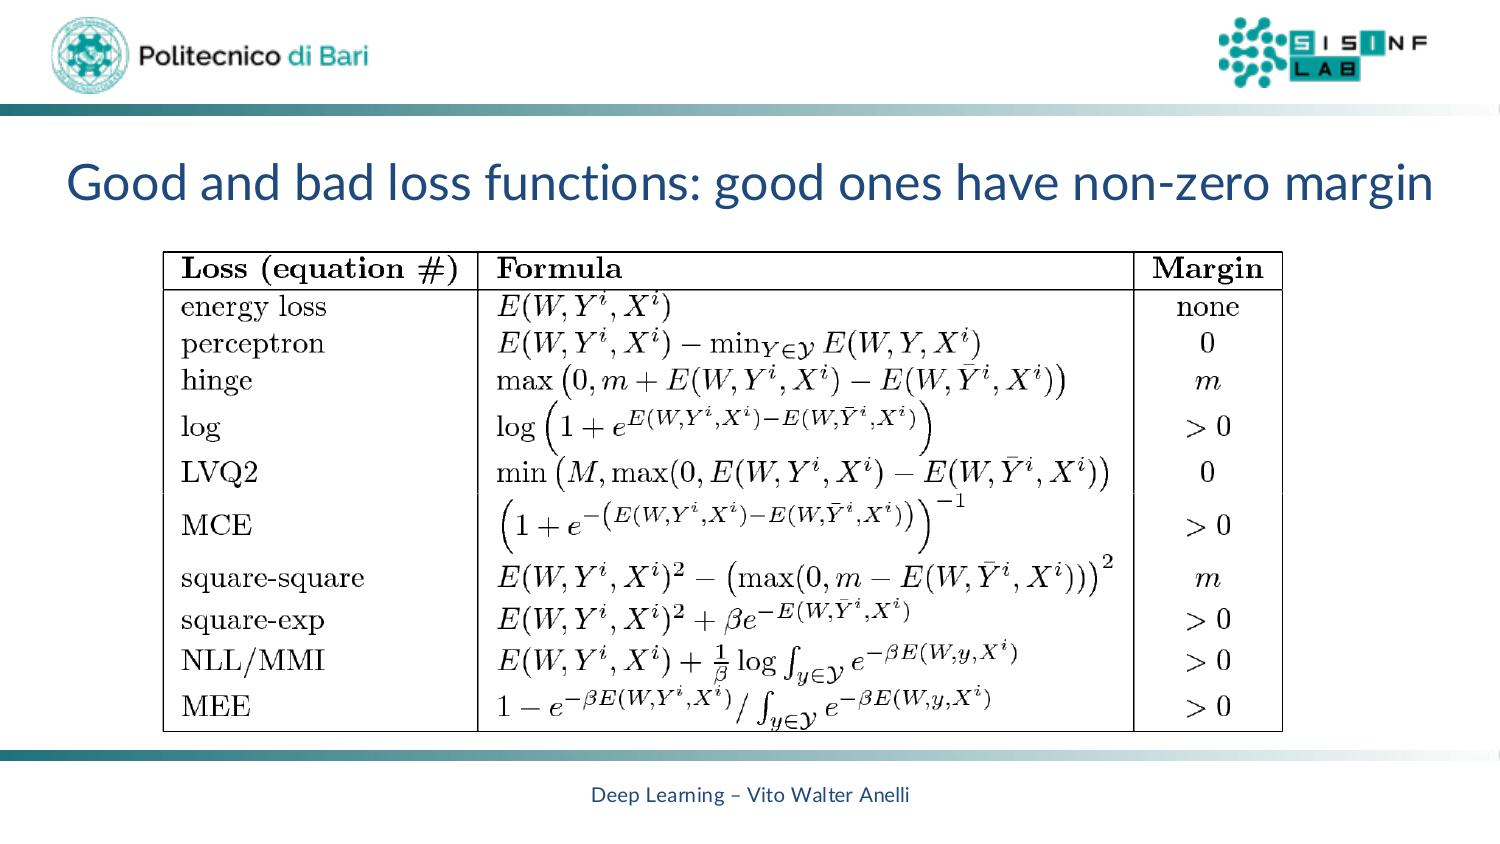
\includegraphics[width=0.90\linewidth]{figures/cf15_loss_functions_table.jpg}
  \caption{Riepilogo delle principali funzioni di perdita per EBM.
           Le perdite con margine non nullo (hinge, square-square,
           MCE, NLL/MMI, MEE, square-exp) sono in genere preferibili
           alla perdita energetica pura e alla perdita percettrone,
           che hanno margine nullo o assente.}
  \label{fig:ebm-loss-functions}
\end{figure}

Le perdite più comuni sono riportate in Tabella~\ref{tab:ebm-losses}.

\begin{table}[H]
  \centering
  \caption{Principali funzioni di perdita per EBM, con relativo margine.
           $E^+\!=\!E(W,Y^i,X^i)$ è l'energia del campione corretto,
           $E^-\!=\!E(W,\bar{Y}^i,X^i)$ è l'energia del campione
           negativo più favorevole.}
  \label{tab:ebm-losses}
  \small
  \begin{tabular}{lll}
    \toprule
    \textbf{Perdita} & \textbf{Formula} & \textbf{Margine} \\
    \midrule
    Energy loss    & $E^+$                                              & nessuno \\
    Perceptron     & $E^+ - \min_{Y\in\mathcal{Y}} E(W,Y,X^i)$          & 0 \\
    Hinge          & $\max(0,\; m + E^+ - E^-)$                         & $m$ \\
    Log            & $\log\!\left(1 + e^{E^+ - E^-}\right)$             & $>0$ \\
    LVQ2           & $\min\!\left(M,\;\max(0,\;E^+ - E^-)\right)$       & 0 \\
    MCE            & $\left(1 + e^{-(E^+ - E^-)}\right)^{-1}$           & $>0$ \\
    Square-square  & $(E^+)^2 - \bigl(\max(0,\;m - E^-)\bigr)^2$        & $m$ \\
    Square-exp     & $(E^+)^2 + \beta\,e^{-E^-}$                        & $>0$ \\
    NLL/MMI        & $E^+ + \frac{1}{\beta}\log\!\int e^{-\beta E}$      & $>0$ \\
    MEE            & $1 - e^{-\beta E^+}\!/\!\int e^{-\beta E}$          & $>0$ \\
    \bottomrule
  \end{tabular}
\end{table}

%------------------------------------------------------------
\section{Joint Embedding Contrastivo}
\label{sec:contrastive-joint-embedding}

Il \textbf{joint embedding contrastivo} combina la struttura a doppio
encoder con la strategia push-down/push-up. Le coppie di campioni sono
di due tipi:

\begin{description}
  \item[Coppia positiva] ($\mathbf{x}$ e $\mathbf{y}$ semanticamente
        equivalenti, ad esempio due viste della stessa immagine): la
        funzione energia $F$ deve essere \emph{piccola}.
  \item[Coppia negativa] ($\mathbf{x}$ e $\mathbf{y}$ semanticamente
        diversi): la funzione energia $F$ deve essere \emph{grande}.
\end{description}

\begin{figure}[H]
  \centering
  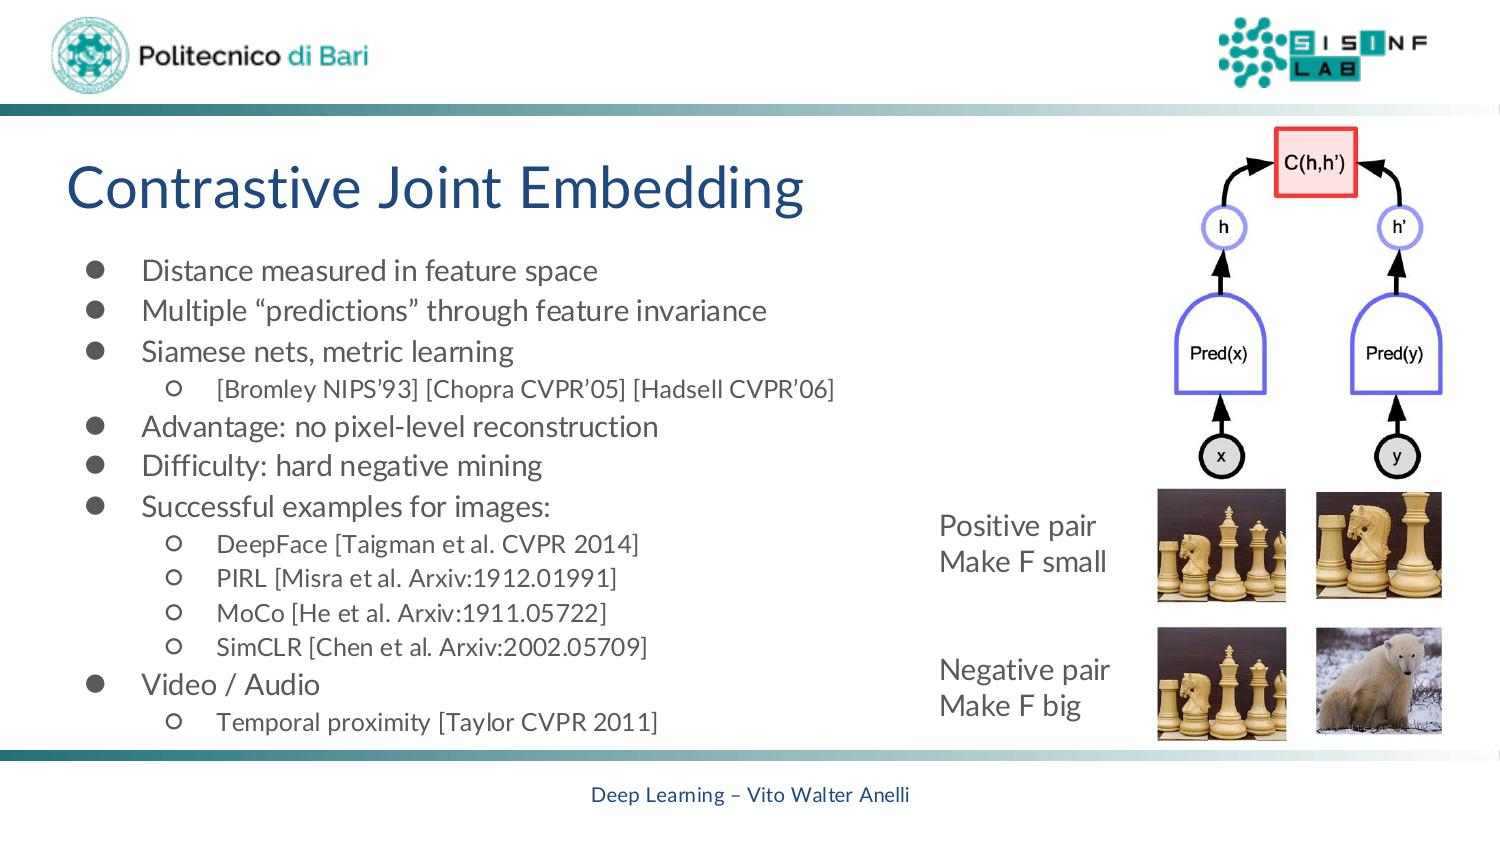
\includegraphics[width=0.85\linewidth]{figures/cf15_contrastive_joint_embedding.jpg}
  \caption{Architettura del joint embedding contrastivo. Due encoder
           $\text{Pred}(x)$ e $\text{Pred}(y)$ proiettano le coppie di
           input nello stesso spazio di feature. La distanza $C(\mathbf{h},
           \mathbf{h}')$ viene minimizzata per le coppie positive (stessa
           scena, diverse prospettive) e massimizzata per le coppie
           negative (scena diversa). Il vantaggio principale è l'assenza
           di ricostruzione pixel-level; la difficoltà principale è il
           \emph{hard negative mining}.}
  \label{fig:contrastive-joint-embedding}
\end{figure}

La principale difficoltà pratica è il \textbf{hard negative mining}: è
necessario identificare campioni negativi sufficientemente informativi
(quelli con bassa energia ma etichetta errata), poiché campioni negativi
facili non forniscono gradiente utile all'addestramento.

\subsection{Joint Embedding Non Contrastivo}
\label{subsec:non-contrastive-embedding}

Per eliminare la necessità di campioni negativi espliciti, i metodi
non contrastivi come \textbf{BYOL}~\citep{grill2020byol}
(\emph{Bootstrap Your Own Latent}, Google DeepMind) e
\textbf{SimSiam}~\citep{chen2021simsiam} adottano una rete siamese
con pesi leggermente diversi tra i due rami. Il ramo \emph{target}
utilizza una media mobile esponenziale (\emph{exponential moving average})
dei pesi del ramo \emph{online}. Questo meccanismo di asimmetria
costituisce un regolarizzatore implicito che impedisce il collasso, senza
richiedere coppie negative.

%------------------------------------------------------------
\section{Self-Supervised Learning}
\label{sec:ssl}

Il \textbf{self-supervised learning} (SSL) risponde alla domanda su come
gli esseri umani e gli animali apprendono a modellare il mondo con
pochissima supervisione esplicita. Nella fase neonatale, l'apprendimento
avviene in larga misura per osservazione: si accumula una quantità
enorme di conoscenza contestuale sulla struttura fisica del mondo
(permanenza degli oggetti, solidity, gravità, inerzia) che costituisce
la base del senso comune.

Nel SSL la \textbf{supervisione è generata autonomamente dai dati stessi}:
si mascherano o corrompono parti dell'input e si addestra il modello a
ricostruirle. Formalmente:
\begin{center}
  \emph{``Predire ogni parte dell'input a partire da tutte le altre.''}
\end{center}

Questo include: predire il futuro dal passato in sequenze temporali,
predire le regioni occultate di un'immagine, completare token mancanti
in una sequenza testuale (come in BERT e GPT).

\subsection{SSL come Riempimento dei Vuoti}
\label{subsec:ssl-fill-blanks}

Il SSL può essere visto come una forma di \emph{riempimento dei vuoti}
(\emph{filling in the blanks}): data una finestra di input, si nasconde
arbitrariamente una porzione (nel tempo, nello spazio, o in entrambi) e
si chiede al modello di predirla. La ricostruzione è un caso speciale di
SSL in cui qualsiasi parte dell'input può essere nota o ignota.

\paragraph{Wav2Vec 2.0.}
Un esempio paradigmatico di SSL applicato al parlato è
\textbf{Wav2Vec 2.0}~\citep{baevski2020wav2vec}: preaddestrato su
960 ore di parlato non etichettato, richiede solo 10 minuti di dati
etichettati per eguagliare le prestazioni del precedente stato dell'arte
che usava 100 ore di etichette. Questo risultato illustra l'efficacia
delle rappresentazioni apprese in modo self-supervised.

\paragraph{Modelli linguistici moderni.}
Nel dominio del testo, i modelli di linguaggio basati su SSL (GPT, BERT,
XLNet, RoBERTa, ALBERT) hanno raggiunto e superato le prestazioni umane
su benchmark di comprensione del testo come il RACE challenge (lettura
tipo SAT), con ALBERT che raggiunge un'accuratezza di 89.4 a fronte di
una baseline umana di circa 95.0 e del precedente SOTA a 83.2.

%------------------------------------------------------------
\section{Connessioni con i Modelli Generativi}
\label{sec:ebm-generative}

\subsection{Relazione con i VAE}
\label{subsec:ebm-vae}

I \textbf{Variational Autoencoders} (VAE) sono un caso speciale di
LV-EBM condizionale in cui il regolarizzatore è la divergenza KL tra la
distribuzione posteriore di $\mathbf{z}$ e una gaussiana standard:
$R(\mathbf{z}) = D_\mathrm{KL}\!\bigl(q(\mathbf{z}|\mathbf{x})
\;\|\; \mathcal{N}(0,I)\bigr)$.
Il rumore aggiunto a $\mathbf{z}$ durante l'addestramento, combinato con
il vincolo sulla norma $\ell_2$, costituisce il meccanismo che limita la
capacità informativa della variabile latente.

\subsection{Confronto con i Metodi Contrastivi e i VAE}
\label{subsec:cd-vs-vae}

\begin{table}[H]
  \centering
  \caption{Confronto tra metodi contrastivi e Variational Autoencoders
           come approcci alternativi per l'addestramento di EBM.}
  \label{tab:cd-vs-vae}
  \small
  \begin{tabular}{lll}
    \toprule
    \textbf{Aspetto}            & \textbf{Metodi Contrastivi}         & \textbf{VAE}                        \\
    \midrule
    Obiettivo principale        & Regolare un EBM                     & Generare dati e apprendere          \\
                                &                                     & una distribuzione esplicita         \\
    Strategia di addestramento  & MCMC per approssimazione            & Discesa del gradiente su ELBO       \\
    Tipo di distribuzione       & Implicita (non parametrica)         & Esplicita (es. gaussiana)           \\
    Efficienza di campionamento & Lenta (più iterazioni MCMC)         & Veloce (spazio latente              \\
                                &                                     & parametrizzato)                     \\
    \bottomrule
  \end{tabular}
\end{table}

%------------------------------------------------------------
\section{Architettura Pratica: ConvNet come EBM}
\label{sec:ebm-convnet}

Un EBM può essere implementato con qualsiasi architettura differenziabile.
Una scelta comune è una \textbf{rete convoluzionale feed-forward} (ConvNet)
che mappa il segnale di input a uno scalare (l'energia). L'architettura
si compone di strati convoluzionali interlacciati con strati di
sottocampionamento, terminando con uno o più strati fully-connected che
producono lo scalare di energia $F(\mathbf{x}, \mathbf{y})$.

Questa configurazione è efficiente poiché sfrutta la condivisione dei
parametri e la località delle connessioni, ed è completamente
differenziabile, consentendo sia l'inferenza per discesa del gradiente
sia l'addestramento tramite backpropagation.

%============================================================
%  Capitolo 16 – Flow Matching e Stable Diffusion 3
%============================================================
\chapter{Flow Matching e Stable Diffusion 3}
\label{ch:flow-matching}

Il \textbf{Flow Matching} (FM) è un paradigma per l'addestramento di
modelli generativi basati su flussi continui normalizzanti (\emph{Continuous
Normalizing Flows}, CNF). Rispetto ai modelli di diffusione classici,
il Flow Matching offre un approccio \emph{simulation-free}: non è
necessario simulare la traiettoria stocastica durante il training, ma
si specifica direttamente il campo vettoriale desiderato e si ottimizzano
i parametri per approssimarlo \citep{lipman2022flow,bishop2024}.

%------------------------------------------------------------
\section{Il Problema della Modellazione Generativa}
\label{sec:fm-generative-problem}

Il problema fondamentale della modellazione generativa consiste nel trovare
una trasformazione $\Phi$ che mappi campioni provenienti da una distribuzione
sorgente $p$ (tipicamente un rumore gaussiano semplice) verso la distribuzione
target $q$ dei dati reali:
\begin{equation}
  X_1 = \Phi(X_0), \qquad X_0 \sim p,\quad X_1 \sim q.
  \label{eq:fm-gen-problem}
\end{equation}
In $\mathbb{R}^d$, ogni immagine (o dato) è un punto, e le distribuzioni
$p$ e $q$ sono insiemi di concentrazione di massa probabilistica nella
stessa spazio ad alta dimensione. Il modello deve imparare a trasportare
la massa da $p$ a $q$.

\subsection{Mappatura Diretta}
\label{subsec:fm-direct-mapping}

L'approccio più immediato è apprendere direttamente la funzione
$X_1 = \Phi(X_0)$ con una rete neurale. Questa strategia ha come
pregio la semplicità e il \textbf{campionamento efficiente} (un solo
forward pass), ma presenta due limiti fondamentali:

\begin{itemize}
  \item Non è intrinsecamente \textbf{probabilistica}: non modella
        esplicitamente la densità della distribuzione target.
  \item Richiede una funzione di perdita \textbf{min-max}, tipicamente
        avversariale (GAN), che è notoriamente instabile durante l'addestramento.
\end{itemize}

\subsection{Processi di Markov a Tempo Continuo}
\label{subsec:fm-ctmp}

Una soluzione più ricca consiste nel modellare la trasformazione come
un \textbf{processo stocastico a tempo continuo} $(X_t)_{0 \le t \le 1}$:
\begin{equation}
  X_{t+h} \leftarrow \Phi_{t+h \mid t}(X_t).
\end{equation}
A seconda della natura dell'operatore di transizione $\Phi_{t+h \mid t}$,
si distinguono tre famiglie principali di processi:

\begin{description}
  \item[\textbf{Flow}] Traiettorie lisce e deterministiche; $\Phi$ è un
        diffeomorfismo.
  \item[\textbf{Diffusione}] Traiettorie stocastiche governate da un'equazione
        differenziale stocastica (SDE); spazio di design più ampio ma
        campionamento più lento.
  \item[\textbf{Jump}] Processi con discontinuità finite; raramente usati
        per dati continui come immagini.
\end{description}

Il \emph{percorso di probabilità marginale} $p_t$ descrive come la
distribuzione marginale dei campioni si trasforma nel tempo:
$X_t \sim p_t$, con $p_0 = p$ e $p_1 = q$.

\begin{figure}[H]
  \centering
  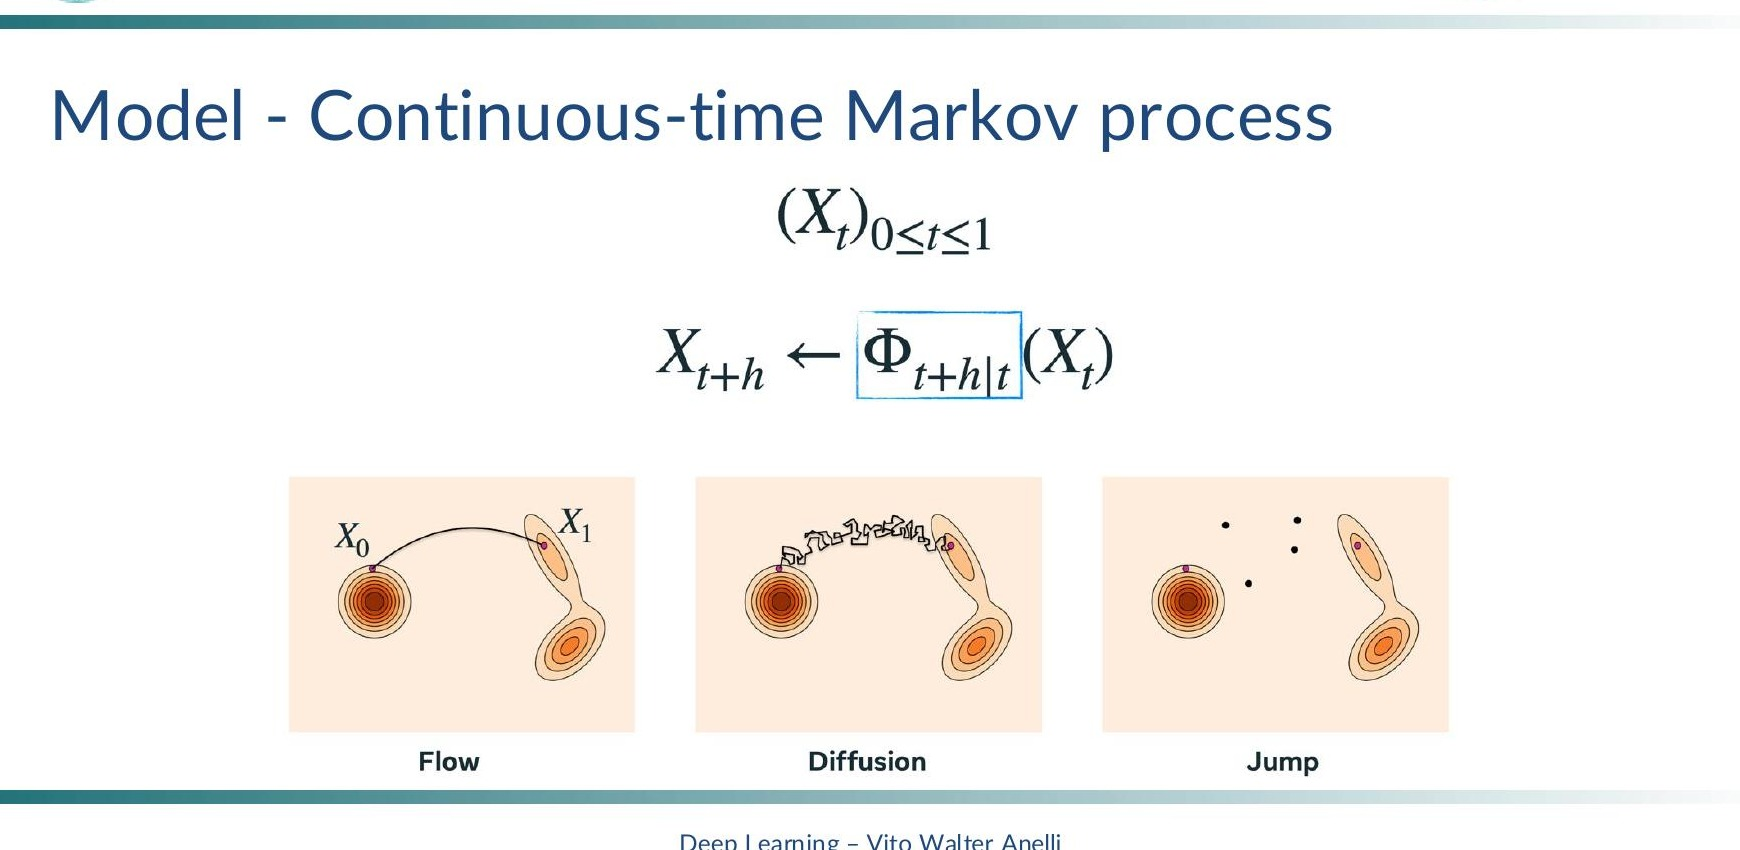
\includegraphics[width=0.82\linewidth]{figures/cf16_ctmp_types.jpg}
  \caption{Le tre famiglie di processi di Markov a tempo continuo.
           \textbf{Flow}: traiettoria liscia e deterministica dal rumore
           al dato. \textbf{Diffusione}: percorso stocastico con
           fluttuazioni browniane. \textbf{Jump}: transizioni discrete
           nello spazio.}
  \label{fig:fm-ctmp-types}
\end{figure}

\subsection{Vantaggi dei Flussi Rispetto alla Diffusione}
\label{subsec:fm-flow-advantages}

I modelli basati su flussi deterministici presentano vantaggi operativi
significativi rispetto ai modelli di diffusione stocastici:

\begin{itemize}
  \item \textbf{Semplicità}: le traiettorie sono lisce e non presentano
        fluttuazioni stocastiche.
  \item \textbf{Campionamento rapido}: è sufficiente risolvere una sola
        ODE, con minor numero di step rispetto alle SDE.
  \item \textbf{Stima esatta della verosimiglianza}: tramite il
        \emph{teorema di cambiamento di variabile} per i flussi continui,
        la log-likelihood è calcolabile in forma chiusa.
  \item \textbf{Flessibilità}: la struttura del flusso è facilmente
        componibile e modificabile.
\end{itemize}

I modelli di diffusione, pur avendo uno spazio di design più ampio,
richiedono in genere la stima di un lower bound (ELBO) della
log-likelihood e un campionamento più lento \citep{ho2020ddpm,bishop2024}.

%------------------------------------------------------------
\section{Flussi, Campi Vettoriali e Velocità}
\label{sec:fm-flows-velocity}

\subsection{Relazione tra Flusso e Campo Vettoriale}
\label{subsec:fm-flow-vector-field}

Un \textbf{campo vettoriale} su $\mathbb{R}^d$ è una funzione
$f : \mathbb{R}^d \to \mathbb{R}^d$ che assegna a ogni punto $x$ dello
\emph{spazio delle fasi} un vettore $v = \dot{x}(t)$. Il
\textbf{campo vettoriale associato al flusso} $\phi_t$ è definito come:
\begin{equation}
  f(x) = \frac{d}{dt}\phi_t(x)\bigg|_{t=0}.
\end{equation}
Poiché $\phi_t(x_0) = x(t)$, il flusso $\phi_t(x)$ è la soluzione al
\textbf{problema ai valori iniziali}:
\begin{equation}
  \frac{d}{dt}\phi_t(x_0) = f\bigl(\phi_t(x_0)\bigr), \qquad \phi_0(x_0) = x_0.
\end{equation}

\subsection{Il Flusso come Funzione di Warping}
\label{subsec:fm-flow-warping}

Un modello generativo basato su flusso apprende una funzione di warping
$\psi_t : \mathbb{R}^d \to \mathbb{R}^d$ parametrizzata da $t \in [0,1]$:
\begin{equation}
  X_t = \psi_t(X_0), \qquad X_0 \sim p, \quad t \in [0,1].
\end{equation}
Il flusso è equivalente, in forma Markoviana, all'aggiornamento:
\begin{equation}
  X_{t+h} = \psi_{t+h \mid t}(X_t).
\end{equation}

La relazione fondamentale tra il flusso $\psi_t$ e la \textbf{velocità}
$u_t$ è data dall'ODE:
\begin{equation}
  \frac{d}{dt}\psi_t(x) = u_t\bigl(\psi_t(x)\bigr).
  \label{eq:fm-ode}
\end{equation}
Dato il flusso, si può ricavare la velocità per differenziazione;
dato il campo di velocità, si può ricavare il flusso integrando l'ODE.

\subsection{Velocità e Distribuzione Marginale}
\label{subsec:fm-velocity-marginal}

Si dice che la velocità $u_t$ \textbf{genera} la distribuzione marginale
$p_t$ se, partendo da campioni $X_0 \sim p$, il processo
$X_t = \psi_t(X_0) \sim p_t$ per ogni $t \in [0,1]$.

\begin{itemize}
  \item \textbf{Pro}: la parametrizzazione tramite velocità è lineare
        rispetto al campo vettoriale (facilita l'apprendimento).
  \item \textbf{Contro}: per generare nuovi campioni è necessario
        simulare (integrare) l'ODE, il che richiede un solutore numerico.
\end{itemize}

\begin{figure}[H]
  \centering
  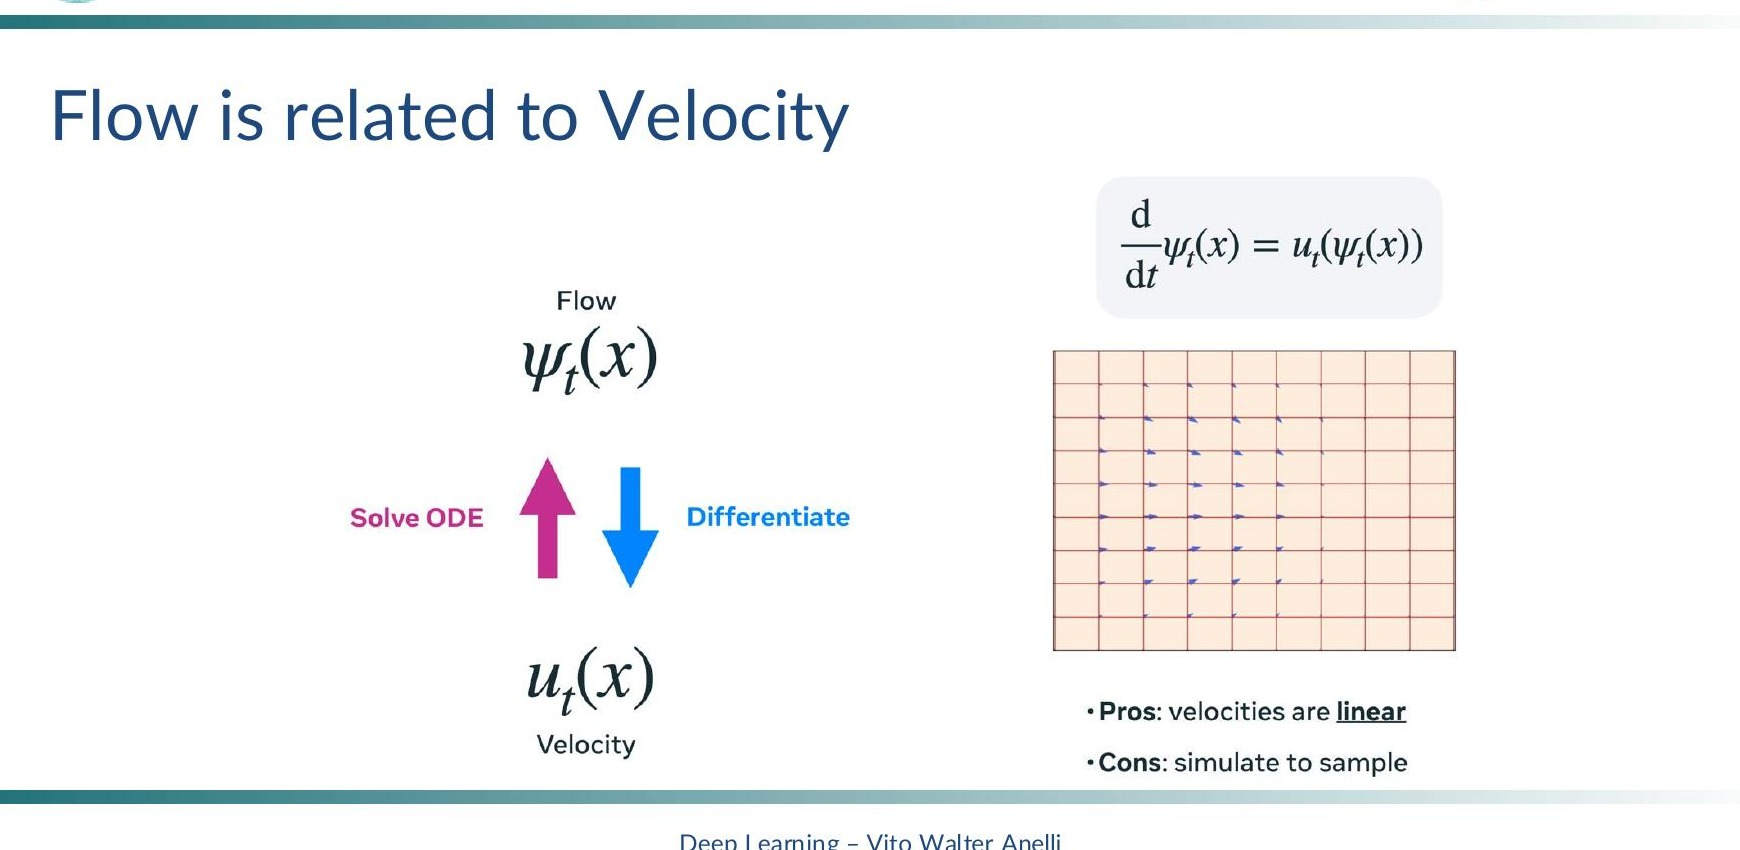
\includegraphics[width=0.72\linewidth]{figures/cf16_velocity_field.jpg}
  \caption{Rappresentazione del campo di velocità $u_t(x)$ su una griglia.
           Ogni freccia indica la direzione e l'intensità dello spostamento
           per i campioni che passano per quella posizione al tempo $t$.}
  \label{fig:fm-velocity-field}
\end{figure}

%------------------------------------------------------------
\section{L'Obiettivo di Flow Matching}
\label{sec:fm-objective}

\subsection{Formulazione Generale}
\label{subsec:fm-general-formulation}

L'idea chiave del Flow Matching è di apprendere una rete neurale
$u_t^\theta : [0,1] \times \mathbb{R}^d \to \mathbb{R}^d$ che approssimi
il campo di velocità marginale $u_t$ capace di trasportare $p_0 = p$ in
$p_1 = q$. Il processo si articola in due fasi:

\begin{enumerate}
  \item \textbf{Training}: minimizzare una funzione di perdita che misura
        la discrepanza tra $u_t^\theta$ e il campo di velocità target.
  \item \textbf{Campionamento}: partire da $X_0 \sim p$ e integrare l'ODE
        $\frac{d}{dt}X_t = u_t^\theta(X_t)$ con un solutore numerico
        (es.\ metodo del punto medio), ottenendo $X_1 \sim q$.
\end{enumerate}

\begin{figure}[H]
  \centering
  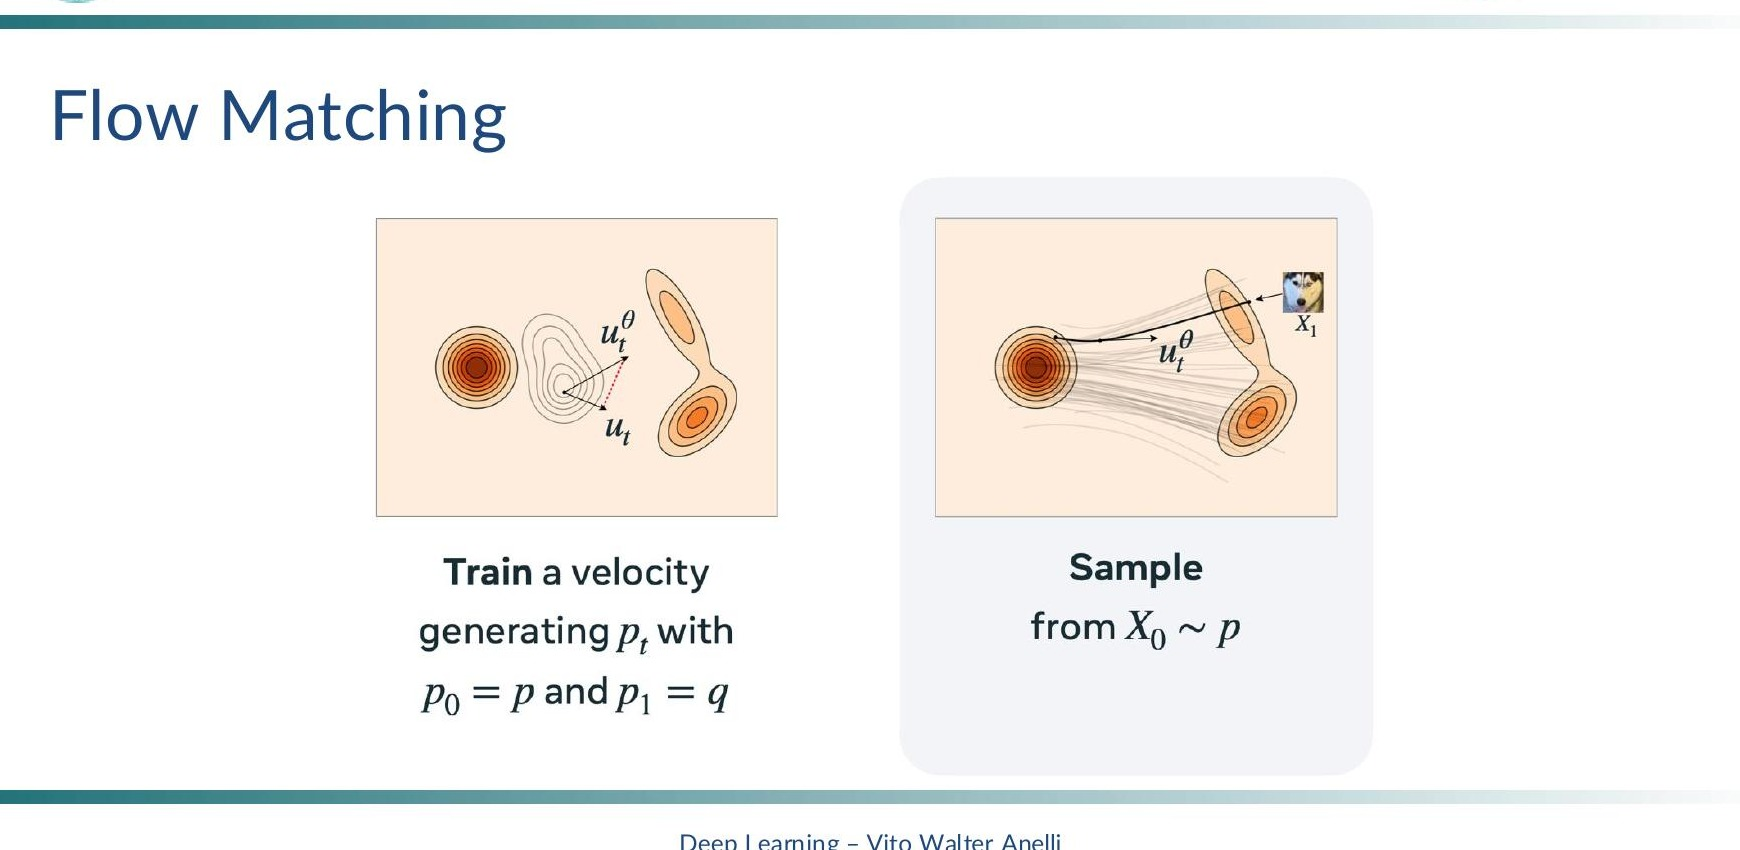
\includegraphics[width=0.85\linewidth]{figures/cf16_fm_train_sample.jpg}
  \caption{Schema di Flow Matching. \textbf{Sinistra}: durante il training,
           la rete $u_t^\theta$ (freccia rossa) viene allineata al campo
           di velocità target $u_t$ (freccia nera). \textbf{Destra}:
           durante il campionamento, le traiettorie sono integrate seguendo
           $u_t^\theta$ a partire da rumore gaussiano $X_0 \sim p$.}
  \label{fig:fm-train-sample}
\end{figure}

\subsection{Versione Più Semplice di Flow Matching}
\label{subsec:fm-simplest-version}

La versione più semplice e pratica del Flow Matching si ottiene
interpolando linearmente tra rumore e dato:
\begin{equation}
  X_t = (1-t)\,X_0 + t\,X_1, \qquad X_0 \sim p,\; X_1 \sim q,
  \label{eq:fm-linear-interp}
\end{equation}
con velocità condizionale costante $u_t(X_t \mid X_1) = X_1 - X_0$.
La funzione di perdita è:
\begin{equation}
  \mathcal{L}(\theta) = \mathbb{E}_{t,\,X_0,\,X_1}\left\|
    u_t^\theta(X_t) - (X_1 - X_0)
  \right\|^2.
  \label{eq:fm-simple-loss}
\end{equation}
In codice PyTorch, il training loop corrispondente è:
\begin{verbatim}
for _ in range(10000):
    x_1 = Tensor(make_moons(256, noise=0.05)[0])
    x_0 = torch.randn_like(x_1)
    t   = torch.rand(len(x_1), 1)
    x_t = (1 - t) * x_0 + t * x_1
    dx_t = x_1 - x_0
    optimizer.zero_grad()
    loss_fn(flow(x_t, t), dx_t).backward()
    optimizer.step()
\end{verbatim}

Il motivo per cui questo funziona risiede nella struttura teorica del
\textbf{Conditional Flow Matching}: il flusso marginale viene costruito
per sovrapposizione di flussi condizionali elementari, ognuno relativo
a un singolo punto target $x_1$.

%------------------------------------------------------------
\section{Flussi Condizionali e il Trucco della Marginalizzazione}
\label{sec:fm-conditional-flows}

\subsection{Costruzione del Flusso da Flussi Condizionali}
\label{subsec:fm-conditional-construction}

Per un singolo punto target $x_1$, si definisce il \textbf{flusso
condizionale}:
\begin{equation}
  X_t = \psi_t(X_0 \mid x_1) = (1-t)\,X_0 + t\,x_1,
\end{equation}
con distribuzione condizionale $p_{t|1}(x \mid x_1)$ e velocità
condizionale $u_t(x \mid x_1)$.

Il flusso e la velocità \textbf{marginali} si ottengono mediando
rispetto alla distribuzione dei dati $q(x_1)$:
\begin{align}
  p_t(x) &= \mathbb{E}_{X_1}\!\left[p_{t|1}(x \mid X_1)\right], \\
  u_t(x) &= \mathbb{E}\!\left[u_t(X_t \mid X_1)\,\Big|\, X_t = x\right].
\end{align}

\subsection{Teorema di Marginalizzazione}
\label{subsec:fm-marginalization-trick}

\begin{theorem}[Marginalizzazione]
La velocità marginale $u_t$ genera il percorso di probabilità marginale
$p_t$. In particolare:
\begin{equation}
  u_t(x) = \mathbb{E}\!\left[u_t(X_t \mid X_1)\,\big|\, X_t = x\right],
  \qquad
  p_t(x) = \mathbb{E}_{X_1}\!\left[p_{t|1}(x \mid X_1)\right].
\end{equation}
\end{theorem}

Questo teorema garantisce che minimizzare la perdita condizionale
\eqref{eq:cfm-loss} sia equivalente a minimizzare la perdita marginale
\eqref{eq:fm-loss}, poiché i loro gradienti rispetto a $\theta$
coincidono.

%------------------------------------------------------------
\section{Funzioni di Perdita per Flow Matching}
\label{sec:fm-losses}

\subsection{Perdita FM e Perdita CFM}
\label{subsec:fm-cfm-losses}

La \textbf{Flow Matching loss} (FM) è:
\begin{equation}
  \mathcal{L}_{\mathrm{FM}}(\theta) =
  \mathbb{E}_{t,\,X_t}\left\|u_t^\theta(X_t) - u_t(X_t)\right\|^2,
  \label{eq:fm-loss}
\end{equation}
dove $u_t$ è il campo di velocità marginale (non direttamente accessibile
in pratica, poiché richiede di conoscere $q$ in forma chiusa).

La \textbf{Conditional Flow Matching loss} (CFM) è:
\begin{equation}
  \mathcal{L}_{\mathrm{CFM}}(\theta) =
  \mathbb{E}_{t,\,X_1,\,X_t}\left\|u_t^\theta(X_t) - u_t(X_t \mid X_1)\right\|^2,
  \label{eq:cfm-loss}
\end{equation}
dove $u_t(x \mid x_1)$ è la velocità condizionale (accessibile per
costruzione tramite la scelta del flusso condizionale).

\begin{theorem}[Equivalenza FM/CFM]
Le due perdite hanno lo stesso gradiente rispetto a $\theta$:
\begin{equation}
  \nabla_\theta\,\mathcal{L}_{\mathrm{FM}}(\theta) =
  \nabla_\theta\,\mathcal{L}_{\mathrm{CFM}}(\theta).
\end{equation}
\end{theorem}

La CFM è quindi trattabile computazionalmente — non richiede
la marginalizzazione esplicita — ed è la perdita usata in pratica.

\subsection{Perdita CFM Generalizzata (Divergenza di Bregman)}
\label{subsec:fm-bregman}

La perdita quadratica può essere generalizzata a qualsiasi
\textbf{divergenza di Bregman} $D$:
\begin{align}
  \mathcal{L}_{\mathrm{FM}}(\theta) &=
    \mathbb{E}_{t,\,X_t}\,D\!\left(u_t(X_t),\, u_t^\theta(X_t)\right), \\
  \mathcal{L}_{\mathrm{CFM}}(\theta) &=
    \mathbb{E}_{t,\,X_1,\,X_t}\,D\!\left(u_t(X_t \mid X_1),\, u_t^\theta(X_t)\right).
\end{align}

\begin{theorem}
  Le due perdite generalizzate sono equivalenti (stessi gradienti) \emph{se
  e solo se} $D$ è una divergenza di Bregman, ovvero:
  \begin{equation}
    \nabla_\theta\,\mathbb{E}_{X,Y}\,D\!\bigl(Y,\, g^\theta(X)\bigr)
    =
    \nabla_\theta\,\mathbb{E}_{X}\,D\!\bigl(\mathbb{E}[Y \mid X],\, g^\theta(X)\bigr).
  \end{equation}
\end{theorem}

%------------------------------------------------------------
\section{Scelta del Flusso Condizionale: Trasporto Ottimale}
\label{sec:fm-ot}

\subsection{Criteri per la Scelta di $\psi_t(x \mid x_1)$}
\label{subsec:fm-ot-criterion}

La scelta del flusso condizionale $\psi_t(x \mid x_1)$ è un grado di
libertà del metodo. La metrica naturale per confrontare le diverse scelte
è l'\textbf{energia cinetica} (KE), ovvero la norma quadrata integrata
del campo di velocità:
\begin{equation}
  \int_0^1 \mathbb{E}_{X_t \sim p_t}\|u_t(X_t)\|^2\,dt
  \;\le\;
  \mathbb{E}_{X_0, X_1}\int_0^1\|\dot\psi_t(X_0 \mid X_1)\|^2\,dt.
\end{equation}

Il \textbf{flusso condizionale lineare} (o \emph{Optimal Transport
condizionale}):
\begin{equation}
  \psi_t(x \mid x_1) = t\,x_1 + (1-t)\,x,
\end{equation}
gode delle seguenti proprietà:
\begin{itemize}
  \item \textbf{Minimizza} il bound sull'energia cinetica.
  \item \textbf{Riduce} l'energia cinetica del coupling iniziale.
  \item È il trasporto ottimale \textbf{esatto} per singoli punti
        (distribuzione di Dirac).
  \item Non è OT nel senso globale, ma produce traiettorie quasi rettilinee
        in alta dimensione.
\end{itemize}

\begin{figure}[H]
  \centering
  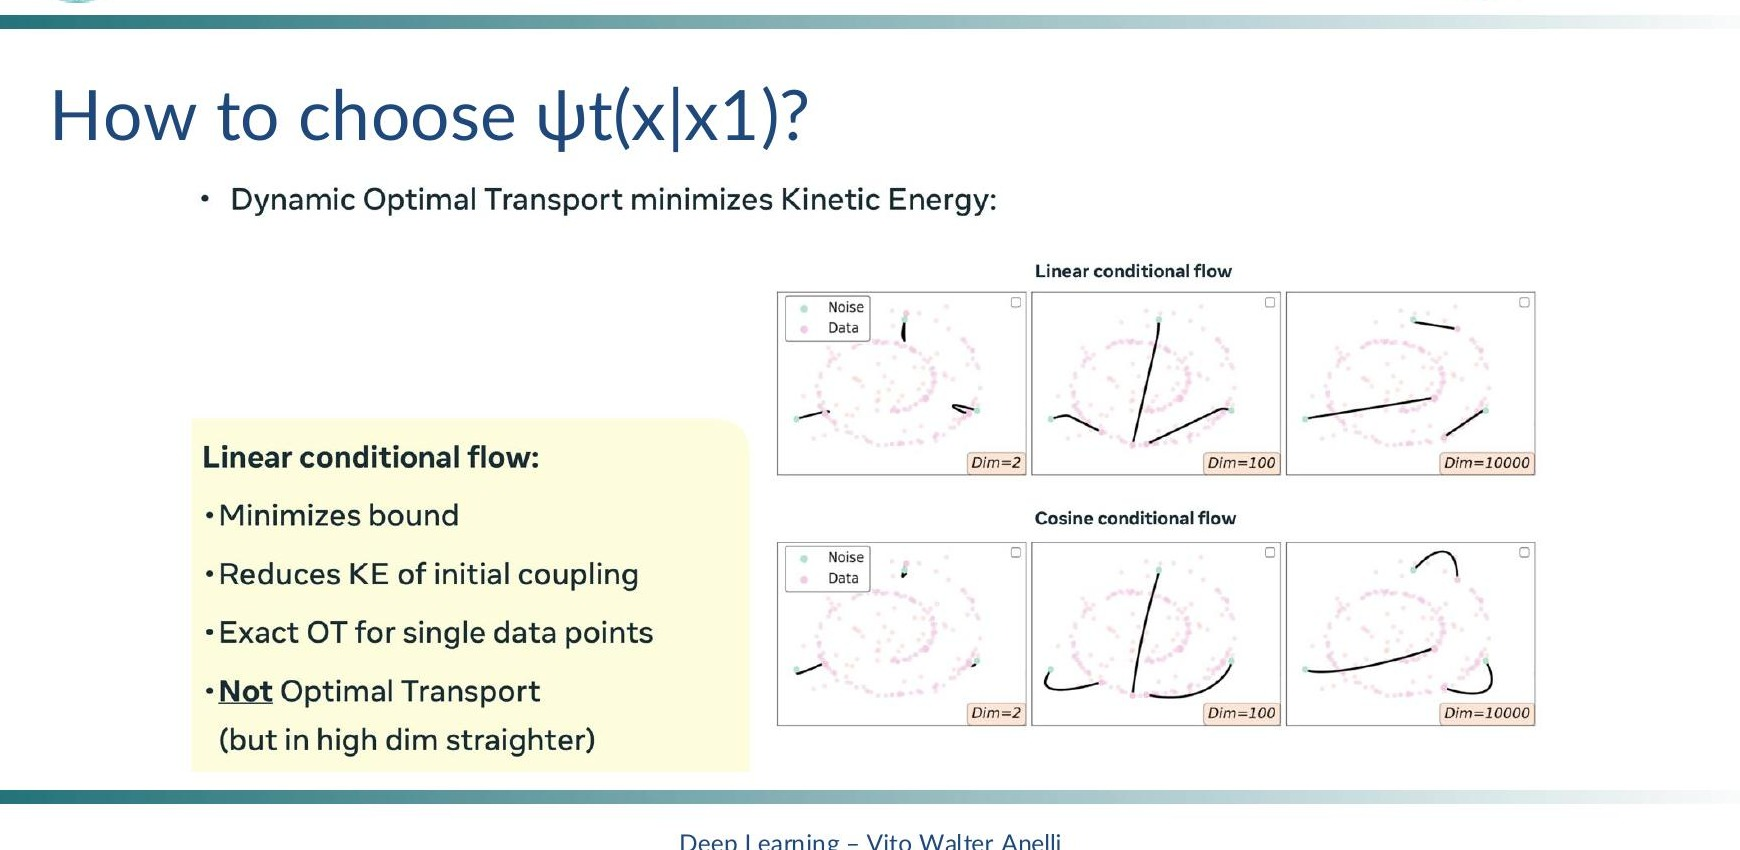
\includegraphics[width=0.88\linewidth]{figures/cf16_linear_vs_cosine.jpg}
  \caption{Confronto tra il flusso condizionale lineare (riga superiore)
           e il flusso condizionale cosinusoidale (riga inferiore) al
           crescere della dimensione ($d=2$, $d=100$, $d=10000$).
           In alta dimensione, le traiettorie lineari si raddrizzano
           sensibilmente, avvicinandosi al trasporto ottimale.}
  \label{fig:fm-linear-vs-cosine}
\end{figure}

\subsection{Flow Matching con Optimal Transport Condizionale}
\label{subsec:fm-cot}

Con la scelta lineare, la perdita CFM diventa:
\begin{align}
  \mathcal{L}_{\mathrm{CFM}}(\theta)
  &= \mathbb{E}\,D\!\left(u_t^\theta(X_t),\; u_t(X_t \mid X_1)\right) \notag\\
  &= \mathbb{E}\left\|u_t^\theta(X_t) - (X_1 - X_0)\right\|^2,
\end{align}
dove $X_t = (1-t)X_0 + tX_1$ e il coupling $(X_0, X_1) \sim \pi_{0,1}$
può essere scelto arbitrariamente (indipendente o strutturato).

%------------------------------------------------------------
\section{Traiettorie Affini e Percorsi Gaussiani}
\label{sec:fm-affine-gaussian}

\subsection{Traiettorie Affini}
\label{subsec:fm-affine}

Una famiglia generale di flussi condizionali è data dai
\textbf{percorsi affini}:
\begin{equation}
  \psi_t(x \mid x_1) = \alpha_t\,x_1 + \sigma_t\,x,
\end{equation}
con $\alpha_0 = 0$, $\alpha_1 = 1$, $\sigma_0 = 1$, $\sigma_1 = 0$
(o varianti con $\sigma_1 \approx 0$ per evitare singolarità).
La velocità corrispondente è:
\begin{equation}
  u_t(x) = \mathbb{E}\!\left[\dot\alpha_t X_1 + \dot\sigma_t X_0 \mid X_t = x\right].
\end{equation}

In questa forma, la velocità ammette tre \textbf{parametrizzazioni
equivalenti}:
\begin{description}
  \item[Predizione di velocità] $u_t(x) = \mathbb{E}[\dot\alpha_t X_1 + \dot\sigma_t X_0 \mid X_t = x]$
  \item[Predizione della sorgente $x_0$] (singolare a $t=0$):
    $u_t(x) = a_t\,x + b_t\,\mathbb{E}[X_0 \mid X_t = x]$
  \item[Predizione del target $x_1$] (singolare a $t=1$):
    $u_t(x) = c_t\,\mathbb{E}[X_1 \mid X_t = x] + d_t$
\end{description}

\subsection{Percorsi Gaussiani e Connessione con la Diffusione}
\label{subsec:fm-gaussian-paths}

Quando la distribuzione sorgente è gaussiana ($p = \mathcal{N}(0, I)$)
e il coupling è indipendente ($\pi_{0,1} = p \cdot q$), i percorsi
affini inducono distribuzioni condizionali gaussiane:
\begin{equation}
  p_{t|1}(x \mid x_1) = \mathcal{N}\!\left(\alpha_t x_1,\; \sigma_t^2 I\right).
\end{equation}
In questo caso, le tre parametrizzazioni della velocità si collegano
direttamente alle formulazioni standard dei modelli di diffusione:

\begin{center}
\begin{tabular}{ll}
  \toprule
  \textbf{Parametrizzazione} & \textbf{Corrispondente nei modelli di diffusione} \\
  \midrule
  Predizione sorgente $x_0$ & Predizione del rumore $\varepsilon$ (\emph{noise prediction}) \\
                             & Probability Flow ODE \\
  Predizione target $x_1$   & Predizione $x_1$ (\emph{denoiser}), $x_1$-prediction \\
  \bottomrule
\end{tabular}
\end{center}

I modelli di diffusione deterministici (es.\ DDIM) sono quindi un caso
speciale di Flow Matching con percorsi Gaussiani, distribuzione sorgente
gaussiana standard, e coupling indipendente \citep{song2020ddim}.

\begin{figure}[H]
  \centering
  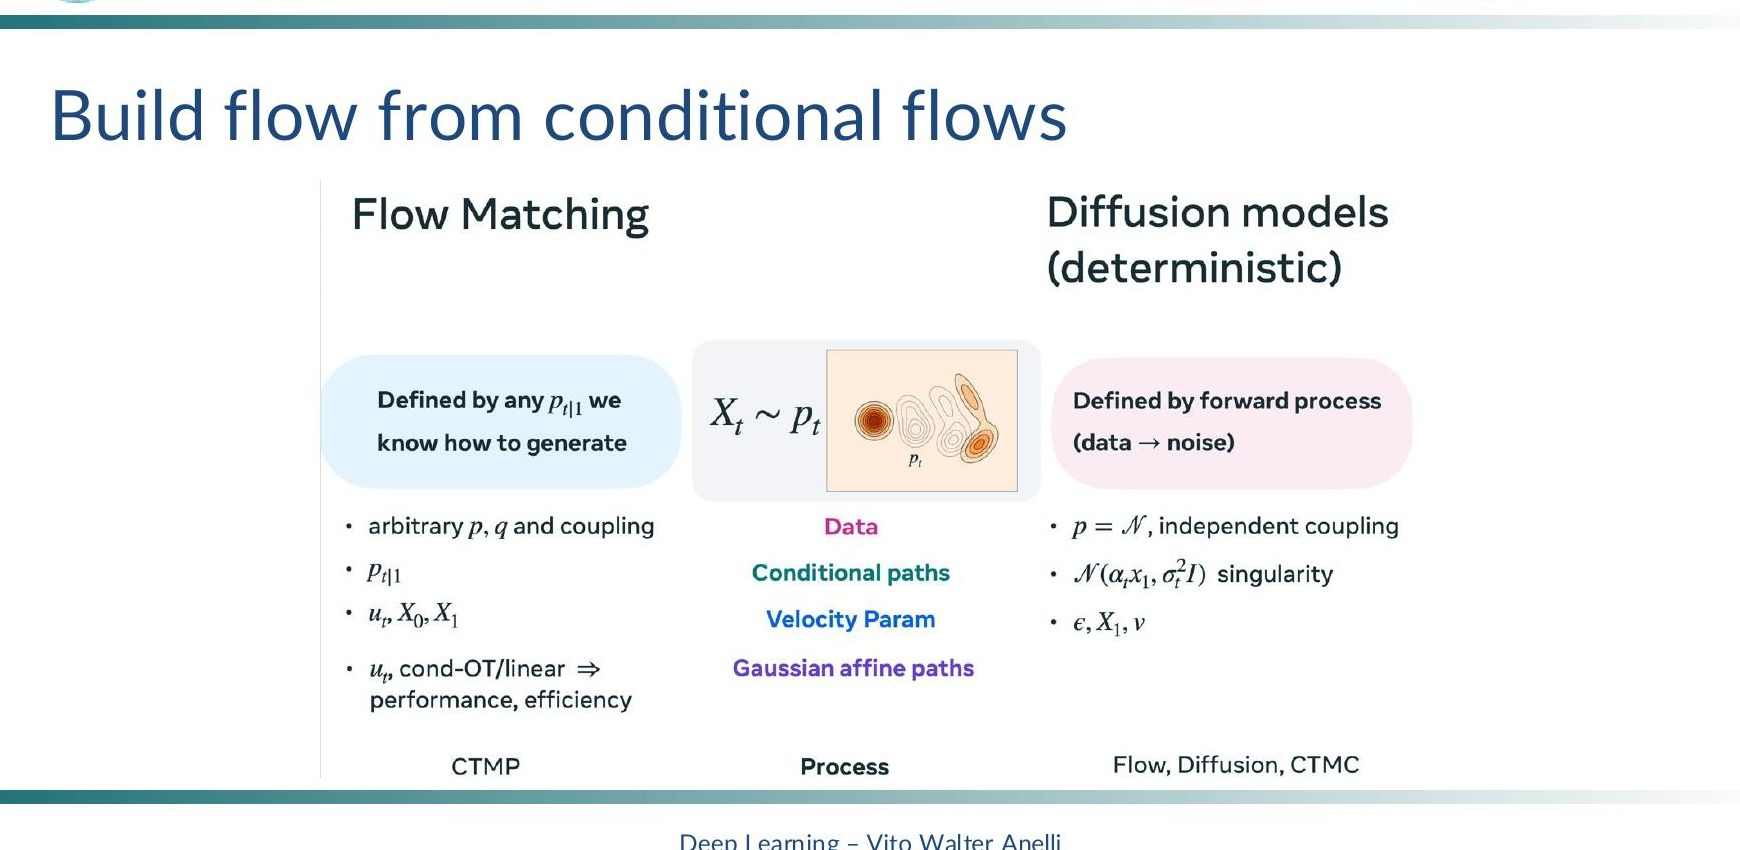
\includegraphics[width=0.82\linewidth]{figures/cf16_fm_vs_diffusion.jpg}
  \caption{Confronto tra Flow Matching e modelli di diffusione deterministici.
           Entrambi operano su processi a tempo continuo, ma si distinguono
           per la scelta del processo condizionale, del coupling e della
           parametrizzazione del campo vettoriale.}
  \label{fig:fm-vs-diffusion}
\end{figure}

%------------------------------------------------------------
\section{Reflow: Raddrizzamento delle Traiettorie}
\label{sec:fm-reflow}

\subsection{Motivazione}
\label{subsec:fm-reflow-motivation}

Anche con il flusso condizionale lineare, le traiettorie integrate
del modello addestrato possono risultare \textbf{curve} (non rettilinee),
perché la rete impara una media ponderata di direzioni che si incrociano.
Traiettorie curve richiedono più step di integrazione per essere
approssimate accuratamente con un solutore numerico, aumentando il costo
di campionamento.

Il \textbf{Reflow} \citep{liu2022flow} è una tecnica che permette di
raddrizzare iterativamente le traiettorie:

\begin{enumerate}
  \item Si inizializza con il flusso lineare standard (traiettorie rette
        ma con incroci durante il training).
  \item Si integra il modello corrente per ottenere coppie $(X_0, \hat X_1)$
        con $\hat X_1 = \text{ODE-solve}(u_t^\theta, X_0)$.
  \item Si riaddestra un nuovo modello FM su queste coppie
        $(\hat X_1, X_0)$, eliminando gli incroci e raddrizzando
        le traiettorie.
\end{enumerate}

\begin{figure}[H]
  \centering
  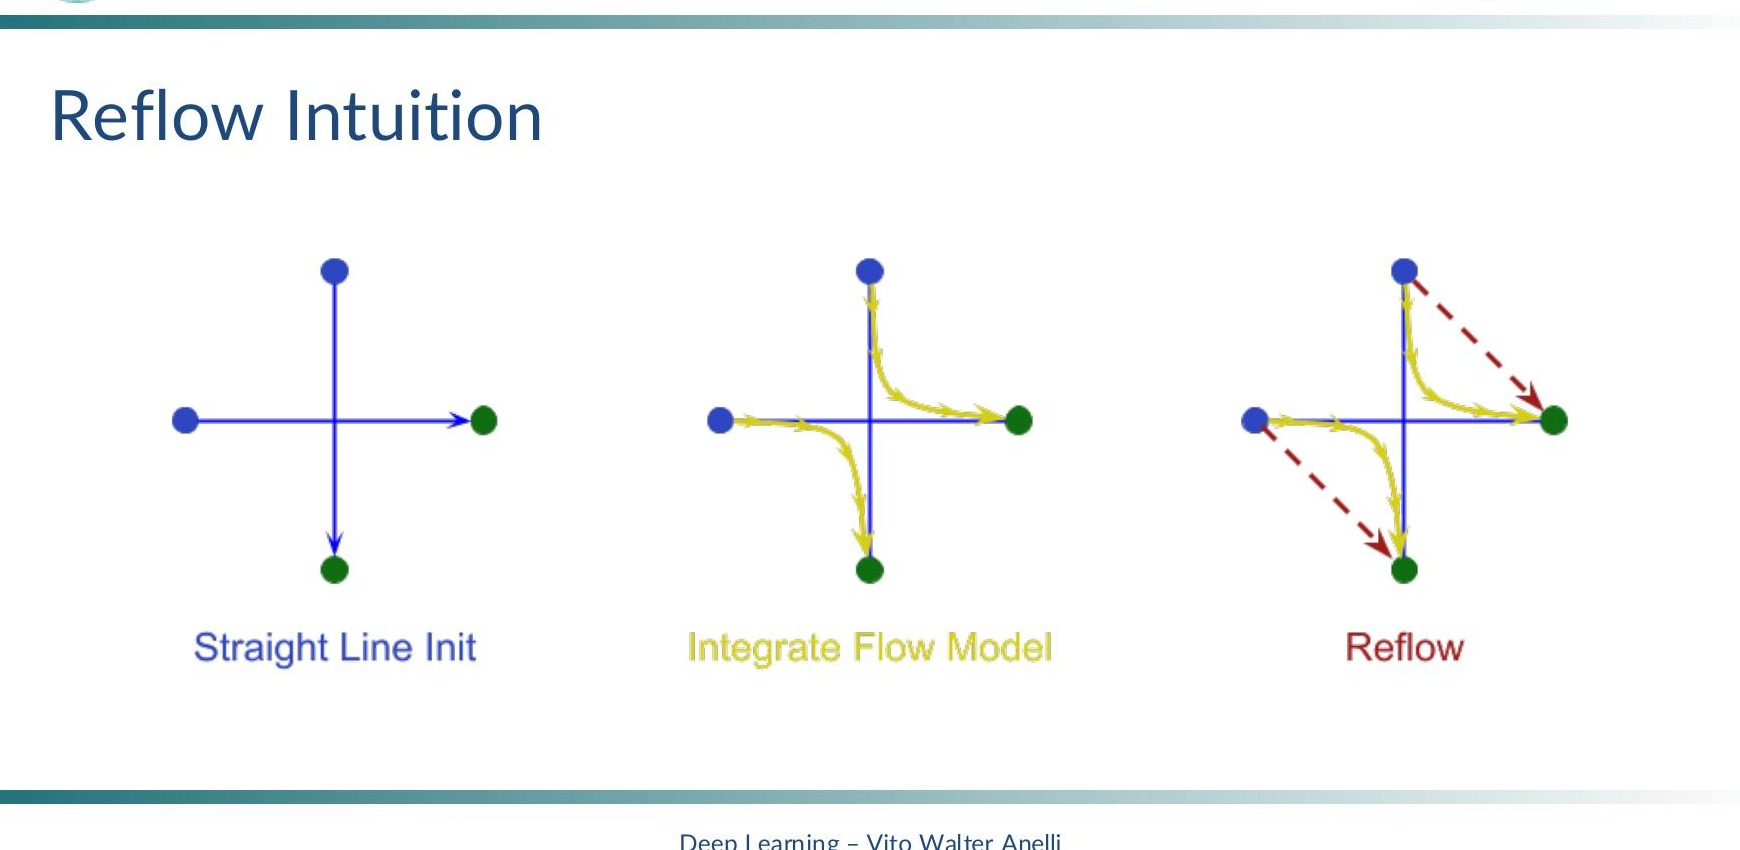
\includegraphics[width=0.85\linewidth]{figures/cf16_reflow_intuition.jpg}
  \caption{Intuizione del Reflow. \textbf{Sinistra}: traiettorie rette ma
           con incroci (initialization lineare). \textbf{Centro}: integrazione
           del modello corrente — le traiettorie si curvano attorno agli
           incroci. \textbf{Destra}: dopo il Reflow, le traiettorie si
           raddrizzano (linee tratteggiate rosse) grazie all'eliminazione
           degli incroci.}
  \label{fig:fm-reflow-intuition}
\end{figure}

\subsection{Effetti del Reflow}
\label{subsec:fm-reflow-effects}

Dopo il Reflow, le traiettorie risultano più rettilinee ma anche più
\textbf{curve globalmente}, a causa della riconfigurazione del campo
vettoriale per evitare incroci. La qualità dei campioni generati rimane
comparabile all'originale, ma l'integrazione può ora essere approssimata
con un minor numero di step (anche un unico step per modelli
sufficientemente reflowed).

%------------------------------------------------------------
\section{Flow Matching Condizionato}
\label{sec:fm-conditioning}

\subsection{Modelli Generativi Condizionali}
\label{subsec:fm-conditional-models}

Nella pratica, si desidera spesso campionare dalla distribuzione condizionale
$q(x_1 \mid y)$, dove $y$ è una condizione (es.\ una caption testuale,
un'etichetta di classe, o un'immagine di riferimento). Si modella un
campo di velocità condizionale:

\begin{align}
  p_{t \mid Y}(x \mid y) &=
    \mathbb{E}_{X_1}\!\left[p_{t|1}(x \mid X_1) \mid Y = y\right], \\
  u_t(x \mid y) &=
    \mathbb{E}\!\left[u_t(X_t \mid X_1) \mid X_t = x,\; Y = y\right].
\end{align}

La perdita di addestramento diventa:
\begin{equation}
  \mathcal{L}_{\mathrm{CFM}}(\theta) =
  \mathbb{E}_{t,\,(X_0, X_1, Y)\sim\pi_{0,1,Y}}\!
  \left\|u_t(X_t \mid X_1) - u_t^\theta(X_t \mid Y)\right\|^2,
\end{equation}
dove la stessa rete $u_t^\theta(x \mid y) : [0,1] \times \mathbb{R}^d \times \mathbb{R}^k \to \mathbb{R}^d$
è addestrata su tutte le condizioni simultaneamente.

\subsection{Guidance per Flow Matching}
\label{subsec:fm-guidance}

Analogamente alla diffusione, esistono due strategie di \emph{guidance}
per orientare il campionamento verso la distribuzione condizionale:

\paragraph{Classifier Guidance.}
Dato un modello incondizionato $u_t(x)$ e un classificatore
$p_{Y|t}(y \mid x)$ addestrato su campioni rumorosi, il campo guidato è:
\begin{equation}
  \tilde{u}_t(x \mid y) = u_t(x) + w\,b_t\,\nabla_x \log p_{Y|t}(y \mid x),
\end{equation}
dove $b_t$ è un fattore di scala che dipende dal percorso Gaussiano e
$w > 0$ è l'intensità della guidance.

\paragraph{Classifier-Free Guidance (CFG).}
Addestrando la stessa rete su condizioni con e senza etichetta
(dropout della condizione durante il training), il campo guidato diventa:
\begin{equation}
  \tilde{u}_t(x \mid y) = (1 - w)\,u_t(x) + w\,u_t(x \mid y).
  \label{eq:fm-cfg}
\end{equation}
Per $w = 1$ si ottiene il modello condizionato puro; per $w > 1$ si
amplifica la condizione a scapito della diversità
\citep{ho2022cfg,bishop2024}.

%------------------------------------------------------------
\section{Multimodal Diffusion Transformers (MMDiT)}
\label{sec:mmdit}

\subsection{Diffusion Transformer (DiT)}
\label{subsec:mmdit-dit}

Il \textbf{Diffusion Transformer} (DiT) \citep{peebles2023dit} è
un'architettura che sostituisce la classica U-Net nei modelli di diffusione
latente con un Transformer puro. I dati rumorosi nel spazio latente
($32 \times 32 \times 4$) vengono suddivisi in patch e proiettati in
token; il timestep $t$ e l'etichetta $y$ vengono iniettati tramite
il meccanismo \textbf{adaLN-Zero} (\emph{adaptive Layer Normalization}):
\begin{equation}
  h \leftarrow \bigl(\mathbf{1} + \gamma_1\bigr)\,\mathrm{LayerNorm}(h) + \beta_1,
\end{equation}
dove $\gamma_1$ e $\beta_1$ sono scalate e traslazioni prodotte da un
MLP che prende in input l'embedding del timestep e dell'etichetta.
Il residuo di attenzione viene modulato da un fattore $\alpha_1$
inizializzato a zero, garantendo che il blocco si riduca all'identità
a inizio training.

\subsection{Multi-Modal Diffusion Transformer (MMDiT)}
\label{subsec:mmdit-mmdit}

Il \textbf{MMDiT} estende il DiT al caso multimodale, consentendo
l'interazione bidirezionale tra sequenze di token eterogenee (es.\
token testuali e token immagine). La chiave architettonica è il
meccanismo di \textbf{Joint Attention}:

\begin{enumerate}
  \item I token di testo e di immagine vengono proiettati separatamente
        in spazi QKV tramite pesi lineari \emph{distinti}.
  \item Le sequenze di Q, K, V vengono concatenate lungo la dimensione
        della sequenza e si calcola un'unica attenzione congiunta.
  \item I risultati vengono separati e restituiti ai rispettivi stream
        (testo e immagine), ciascuno modulato indipendentemente.
\end{enumerate}

\begin{figure}[H]
  \centering
  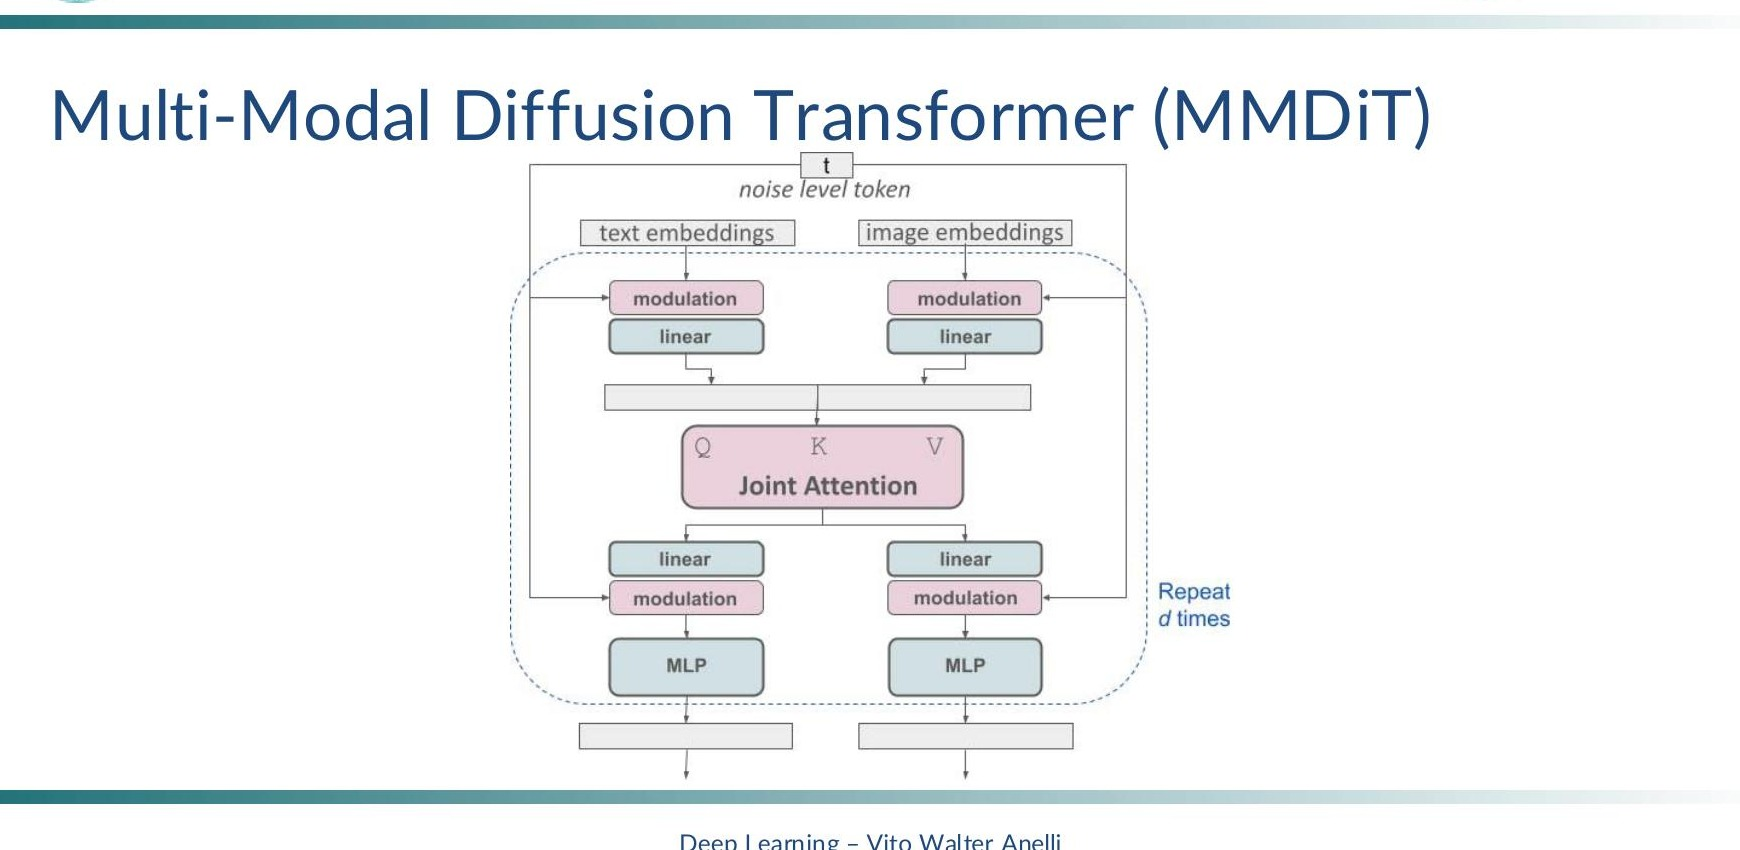
\includegraphics[width=0.65\linewidth]{figures/cf16_mmdit_block.jpg}
  \caption{Un blocco MM-DiT. I due stream (testo a sinistra, immagine a
           destra) condividono il meccanismo di attenzione congiunta
           (Joint Attention) ma mantengono pesi lineari e modulation MLP
           separati. Il token di livello di rumore $t$ modula entrambi
           gli stream tramite il meccanismo adaLN.}
  \label{fig:mmdit-block}
\end{figure}

%------------------------------------------------------------
\section{Stable Diffusion 3}
\label{sec:sd3}

\subsection{Architettura Complessiva}
\label{subsec:sd3-architecture}

\textbf{Stable Diffusion 3} (SD3) \citep{esser2024sd3} è un modello
testo-immagine allo stato dell'arte che combina Flow Matching con
l'architettura MMDiT. I componenti principali sono:

\begin{description}
  \item[\textbf{Text Encoders}] Tre encoder testuali in parallelo:
    CLIP-G/14, CLIP-L/14 e T5 XXL. I token contestuali di CLIP-L e
    CLIP-G (77+77 token) vengono concatenati lungo i canali e proiettati
    in 4096 dimensioni come condizione testuale $c$. I pooled embedding
    di CLIP-G/14 vengono sommati all'embedding del timestep per formare
    il vettore di condizione globale $y$.
  \item[\textbf{Latent VAE}] Il \emph{Noised Latent} è ottenuto
    codificando l'immagine in uno spazio latente tramite un VAE
    (risoluzione ridotta), aggiungendo rumore gaussiano, e poi
    patchificando il risultato tramite una proiezione lineare.
  \item[\textbf{Positional Embedding}] Embedding posizionale 2D sommato
    ai token immagine prima dei blocchi MM-DiT.
  \item[\textbf{MM-DiT Blocks}] Una sequenza di $d$ blocchi MM-DiT
    che elaborano congiuntamente token testuali e immagine, aggiornati
    entrambi a ogni layer.
  \item[\textbf{Output}] Dopo gli $d$ blocchi, un layer di
    modulazione e una proiezione lineare producono il campo di velocità
    stimato; il risultato viene de-patchificato per ricostruire la
    predizione nel spazio latente.
\end{description}

\begin{figure}[H]
  \centering
  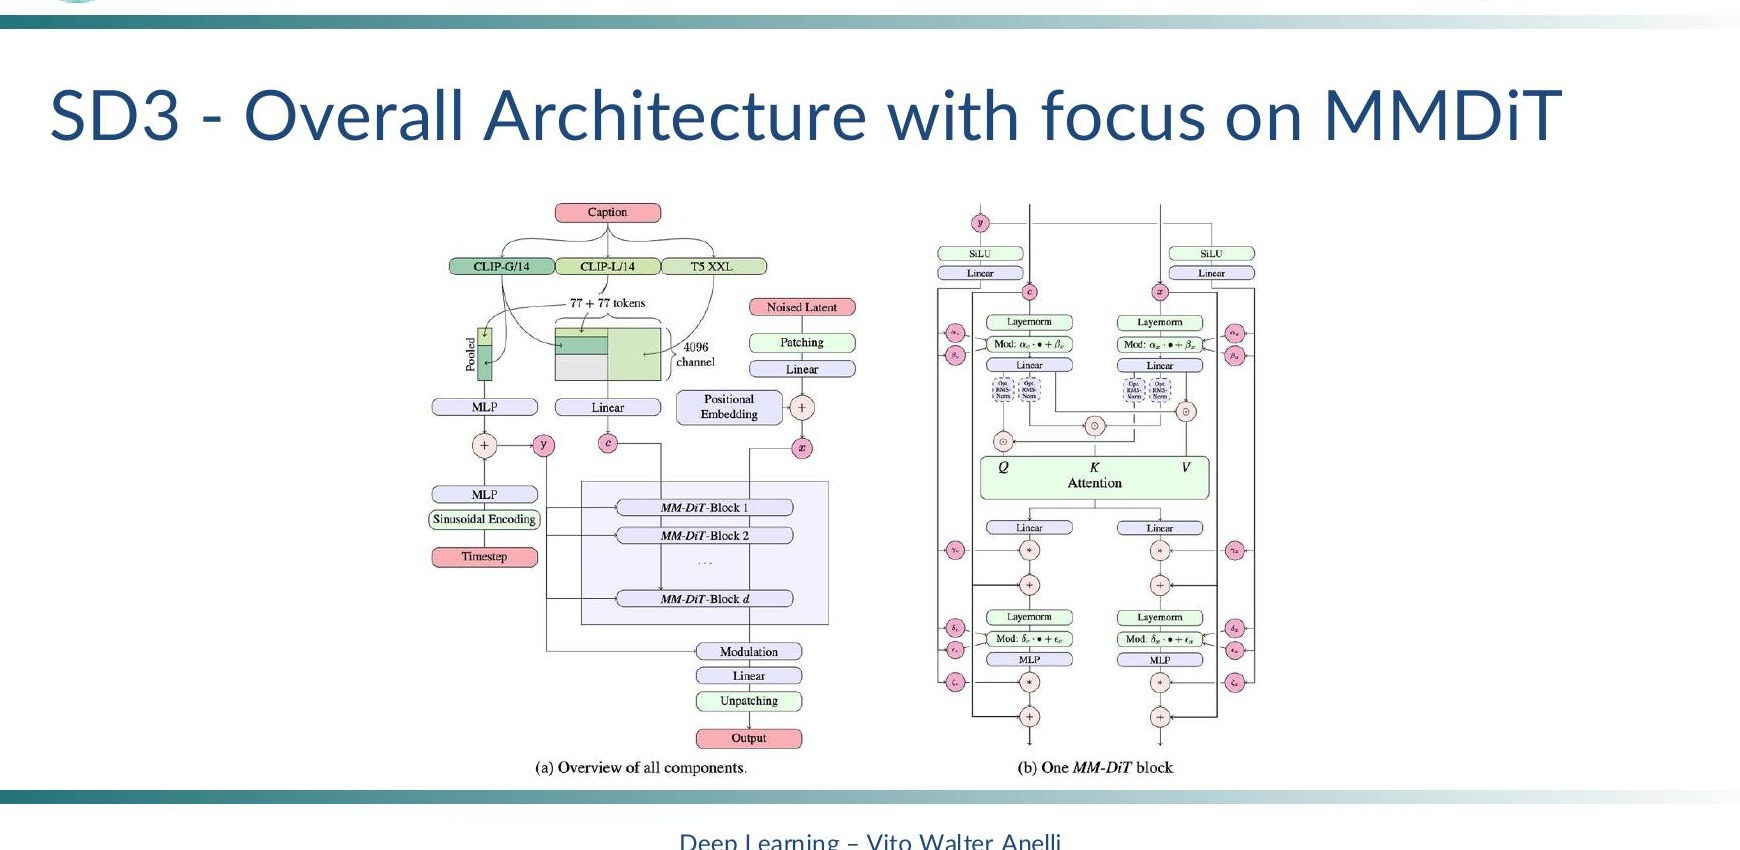
\includegraphics[width=0.88\linewidth]{figures/cf16_sd3_architecture.jpg}
  \caption{Architettura completa di Stable Diffusion 3. Il percorso
           superiore elabora la caption testuale tramite tre encoder
           (CLIP-G/14, CLIP-L/14, T5 XXL) e produce gli embedding
           contestuali $c$ e globali $y$. Il percorso inferiore processa
           il latent rumoroso con patchify e positional embedding. Entrambi
           i flussi di informazione vengono elaborati congiuntamente
           all'interno dei blocchi MM-DiT, iterati $d$ volte.}
  \label{fig:sd3-architecture}
\end{figure}

\subsection{Il Ruolo di T5 in SD3}
\label{subsec:sd3-t5}

\textbf{T5} (\emph{Text-To-Text Transfer Transformer}) \citep{raffel2020t5}
è un modello encoder-decoder basato su Transformer che inquadra qualsiasi
compito NLP come un problema testo-a-testo. In SD3, viene utilizzata la
variante \textbf{T5 XXL} come encoder testuale, per la sua capacità di
rappresentare testi con semantica ricca e dipendenze a lunga distanza.

Le caratteristiche architetturali principali di T5 sono:

\begin{itemize}
  \item \textbf{Relative Positional Embeddings} con bias scalare aggiunto
        alla matrice di attenzione: $A_{ij} \leftarrow A_{ij} + b(i-j)$.
  \item \textbf{Pre-LayerNorm}: la normalizzazione è applicata
        \emph{all'ingresso} di ogni blocco (non all'uscita come in BERT),
        con una variante ``scale-only'' (RMSNorm senza bias).
  \item \textbf{Pre-training con Span Corruption}: porzioni contigue di
        token vengono mascherate e il modello viene addestrato a
        ricostruirle, un'estensione del Masked Language Model a span
        interi (anziché token singoli come in BERT).
  \item \textbf{Attenzione Causale con Prefisso} (\emph{Prefix LM}):
        la sequenza di input usa attenzione bidirezionale, mentre la
        sequenza di output usa attenzione causale (unidirezionale).
\end{itemize}

T5 è stato pre-addestrato sul dataset \textbf{C4} (\emph{Colossal Clean
Crawled Corpus}) con un obiettivo di denoising, e poi fine-tuned su
molteplici task (GLUE, SuperGLUE, SQuAD, WMT) usando un approccio
multi-task unificato. In SD3, solo l'encoder T5 viene utilizzato: i
suoi output token vengono concatenati con quelli di CLIP e usati come
condizione testuale nel MMDiT.

\subsection{Formazione del Modello e Scelte di Design}
\label{subsec:sd3-training}

Le principali scelte di design che distinguono SD3 dai predecessori sono:

\paragraph{Flow Matching con OT condizionale.}
SD3 utilizza la formulazione lineare di Flow Matching ($X_t = (1-t)X_0 + tX_1$)
con coupling indipendente, che produce traiettorie quasi rettilinee in
alta dimensione e permette un campionamento efficiente con pochi step.

\paragraph{Architettura MMDiT scalabile.}
Il design con stream separati per testo e immagine, ma attenzione
congiunta, permette di scalare i pesi del modello in modo efficiente:
si può raddoppiare la profondità del modello senza modificare le
interfacce tra le componenti.

\paragraph{Tre encoder testuali complementari.}
CLIP-G e CLIP-L catturano relazioni semantiche visivo-testuali globali;
T5 XXL cattura strutture linguistiche complesse e descrizioni testuali
dettagliate. La combinazione migliora la fedeltà al testo rispetto all'uso
di un solo encoder.

%------------------------------------------------------------
\section{Procedura di Addestramento e Campionamento}
\label{sec:fm-training-sampling}

\subsection{Procedura di Training}
\label{subsec:fm-training}

L'addestramento di un modello Flow Matching segue i seguenti passi ad
ogni iterazione:

\begin{enumerate}
  \item \textbf{Campionare} coppie $(X_0, X_1)$ dalla distribuzione
        sorgente $p$ e dalla distribuzione target $q$ (eventualmente
        con un coupling strutturato $\pi_{0,1}$).
  \item \textbf{Campionare} un tempo $t \sim \mathrm{Uniform}[0,1]$.
  \item \textbf{Calcolare} la posizione interpolata
        $X_t = (1-t)X_0 + tX_1$ — dove il punto si troverebbe se si
        muovesse a velocità costante da $X_0$ a $X_1$.
  \item \textbf{Calcolare} la velocità target $\dot X_t = X_1 - X_0$
        (costante lungo la traiettoria lineare).
  \item \textbf{Aggiornare} i parametri $\theta$ minimizzando
        $\|u_t^\theta(X_t) - (X_1 - X_0)\|^2$. La rete impara la
        ``media'' delle velocità di tutti i punti che passano per
        $X_t$ al tempo $t$.
\end{enumerate}

L'approccio è \textbf{simulation-free}: a differenza dei modelli di
diffusione che richiedono l'integrazione dell'SDE durante il training,
il Flow Matching non richiede mai di simulare la traiettoria.

\subsection{Campionamento}
\label{subsec:fm-sampling}

Per generare un campione:
\begin{enumerate}
  \item Campionare $X_0 \sim \mathcal{N}(0, I)$.
  \item Integrare l'ODE $\frac{d}{dt}X_t = u_t^\theta(X_t)$
        da $t=0$ a $t=1$ con un solutore numerico
        (es.\ metodo di Eulero, metodo del punto medio o Runge-Kutta 4).
  \item Restituire $X_1$ come campione dalla distribuzione target.
\end{enumerate}

Il metodo del \textbf{punto medio} (Heun/RK2) è particolarmente adatto
in quanto offre un buon compromesso tra accuratezza e costo computazionale.
Con traiettorie sufficientemente rettilinee (ottenute con OT condizionale
o Reflow), anche un singolo step di Eulero può produrre campioni di
buona qualità.

%------------------------------------------------------------
\section{Connessioni con Altri Modelli Generativi}
\label{sec:fm-connections}

\begin{table}[H]
  \centering
  \caption{Confronto tra Flow Matching, modelli di diffusione e approcci
           diretti. FM = Flow Matching, DDPM = Denoising Diffusion
           Probabilistic Model, DDIM = Denoising Diffusion Implicit Model,
           OT-CFM = Conditional OT Flow Matching.}
  \label{tab:fm-comparison}
  \small
  \adjustbox{max width=\linewidth}{%
  \begin{tabular}{lccccc}
    \toprule
    \textbf{Aspetto}
      & \textbf{FM/OT-CFM}
      & \textbf{DDPM}
      & \textbf{DDIM}
      & \textbf{GAN}
      & \textbf{VAE} \\
    \midrule
    Simulation-free training & \checkmark & \checkmark & \checkmark & \checkmark & \checkmark \\
    Traiettorie rettilinee   & \checkmark & $\times$  & $\times$  & n/a & n/a \\
    Verosimiglianza esatta   & \checkmark & $\times$  & $\times$  & $\times$ & $\approx$ \\
    Campionamento efficiente & \checkmark & $\times$  & $\approx$ & \checkmark & \checkmark \\
    Coupling arbitrario      & \checkmark & $\times$  & $\times$  & $\times$ & $\times$ \\
    Stabilità di training    & alta & alta & alta & bassa & alta \\
    \bottomrule
  \end{tabular}%
  }
\end{table}

In sintesi, il Flow Matching unifica e generalizza i modelli di diffusione
deterministici (DDIM) come caso speciale con percorsi Gaussiani e coupling
indipendente, mentre aggiunge la flessibilità di scegliere coupling
arbitrari (es.\ mini-batch OT) e percorsi non Gaussiani, con il vantaggio
computazionale di traiettorie tendenzialmente più rettilinee e quindi
campionamento più rapido \citep{lipman2022flow,liu2022flow,albergo2022building,bishop2024}.

%============================================================
%  Capitolo 17 – Advanced Multi-Head Attention
%============================================================
\chapter{Advanced Multi-Head Attention}
\label{ch:advanced-attention}

I modelli linguistici di grandi dimensioni (\emph{Large Language Models}, LLM)
basati su Transformer generano token in modo \textbf{autoregressivo}: ad ogni
passo $t$ viene prodotto un singolo token, dato tutti quelli precedenti.
L'operazione di Self-Attention domina il costo computazionale e di memoria
di questa fase di inferenza. In questo capitolo vengono analizzate le
principali ottimizzazioni architetturali sviluppate per ridurre il costo
della memoria e migliorare l'efficienza dell'inferenza, mantenendo al
contempo una qualità del modello comparabile o superiore alla Multi-Head
Attention standard \citep{vaswani2017attention,bishop2024}.

%------------------------------------------------------------
\section{KV Cache}
\label{sec:kv-cache}

\subsection{Riepilogo della Multi-Head Attention}
\label{subsec:mha-recap}

Nella Multi-Head Attention (MHA) standard, dati i vettori di input
$\mathbf{x}_1, \ldots, \mathbf{x}_s \in \mathbb{R}^{d_{\text{model}}}$
(con $s$ lunghezza della sequenza), per ciascun head $i = 1,\ldots,n$ vengono
calcolate le proiezioni:
\begin{align}
  Q_i &= X W_Q^{(i)}, \quad K_i = X W_K^{(i)}, \quad V_i = X W_V^{(i)},
\end{align}
dove $X \in \mathbb{R}^{s \times d_{\text{model}}}$ è la matrice degli
embedding di input e $W_Q^{(i)}, W_K^{(i)}, W_V^{(i)} \in
\mathbb{R}^{d_{\text{model}} \times d_h}$ sono le matrici di proiezione del
$i$-esimo head, con $d_h = d_{\text{model}} / n$ dimensione del singolo head.

Il punteggio di attenzione per il head $i$ è:
\begin{equation}
  \text{Attention}(Q_i, K_i, V_i) = \text{Softmax}\!\left(
    \frac{Q_i K_i^\top}{\sqrt{d_h}}
  \right) V_i.
  \label{eq:sdpa}
\end{equation}
Le uscite di tutti gli head vengono concatenate e proiettate:
\begin{equation}
  \text{MHA}(X) = \bigl[\text{head}_1;\ldots;\text{head}_n\bigr] W_O,
  \qquad W_O \in \mathbb{R}^{d_{\text{model}} \times d_{\text{model}}}.
\end{equation}
Nell'attenzione \textbf{mascherata} (causale), utilizzata nei modelli decoder,
la matrice di attenzione è una matrice triangolare inferiore: il token in
posizione $t$ può attendere solo ai token nelle posizioni $1, \ldots, t$,
impedendo la visione anticipata dei token futuri.

\subsection{Computazione a ogni passo autoregressivo}
\label{subsec:autoregressive-step}

Durante la generazione autoregressiva, al passo $t$ si conosce solo il nuovo
token $\mathbf{x}_t$. Tuttavia, per calcolare i punteggi di attenzione
rispetto a tutti i token precedenti, è necessario disporre di:
\begin{itemize}
  \item la \textbf{Query} del token corrente: $\mathbf{q}_t = \mathbf{x}_t W_Q$,
  \item le \textbf{Key} di tutti i token $1,\ldots,t$: $K_{1:t} = X_{1:t} W_K$,
  \item i \textbf{Value} di tutti i token $1,\ldots,t$: $V_{1:t} = X_{1:t} W_V$.
\end{itemize}
Le matrici di Key e Value si ricavano moltiplicando l'intera sequenza di
embedding $X_{1:t}$ per i rispettivi pesi. Ricalcolare queste proiezioni
ad ogni nuovo token è \textbf{computazionalmente ridondante}: i token
$1, \ldots, t{-}1$ non cambiano tra un passo e l'altro.

\subsection{Meccanismo della KV Cache}
\label{subsec:kv-cache-mechanism}

La \textbf{KV Cache} (Key-Value Cache) è una tecnica di memoizzazione che
consiste nel conservare in memoria le proiezioni Key e Value già calcolate
nei passi precedenti, evitando di ricalcolarle ad ogni step. Formalmente,
si mantiene in memoria la struttura:
\begin{equation}
  \text{KV Cache} = \bigl\{(K_{1:t-1},\, V_{1:t-1})\bigr\}
  \quad \text{per ogni layer e ogni head.}
\end{equation}
Ad ogni nuovo passo $t$:
\begin{enumerate}
  \item Si calcolano solo $\mathbf{k}_t = \mathbf{x}_t W_K$ e
        $\mathbf{v}_t = \mathbf{x}_t W_V$ per il token corrente.
  \item Si aggiunge $(\mathbf{k}_t, \mathbf{v}_t)$ alla cache.
  \item Si usa la cache completa $K_{1:t}, V_{1:t}$ per calcolare
        l'attenzione con la query $\mathbf{q}_t$.
\end{enumerate}
In questo modo il costo computazionale per passo è $O(s \cdot d_h)$ invece
di $O(s^2 \cdot d_h)$.

\begin{figure}[H]
  \centering
  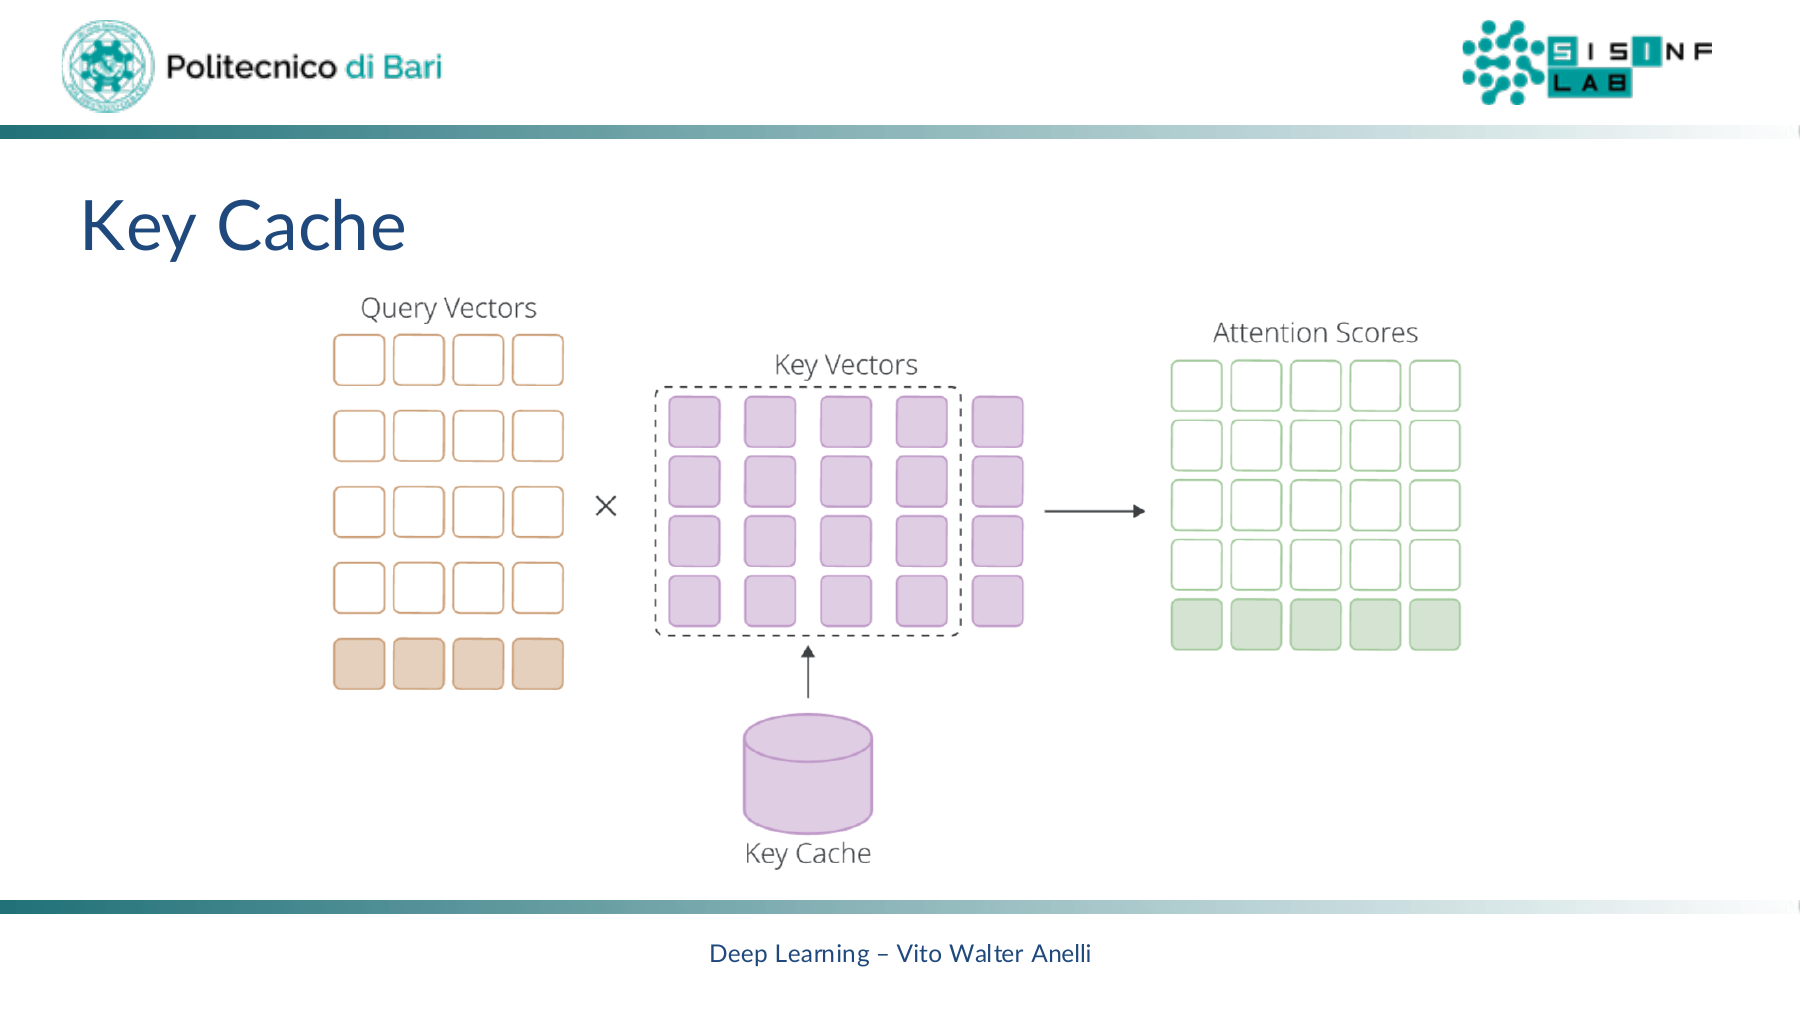
\includegraphics[width=0.80\linewidth]{figures/cf17_key_cache.png}
  \caption{Meccanismo della Key Cache. I vettori chiave dei token precedenti
           sono recuperati dalla cache (cilindro) ed usati direttamente nel
           prodotto scalare con il query del token corrente (riga arancione).}
  \label{fig:key-cache}
\end{figure}

\begin{figure}[H]
  \centering
  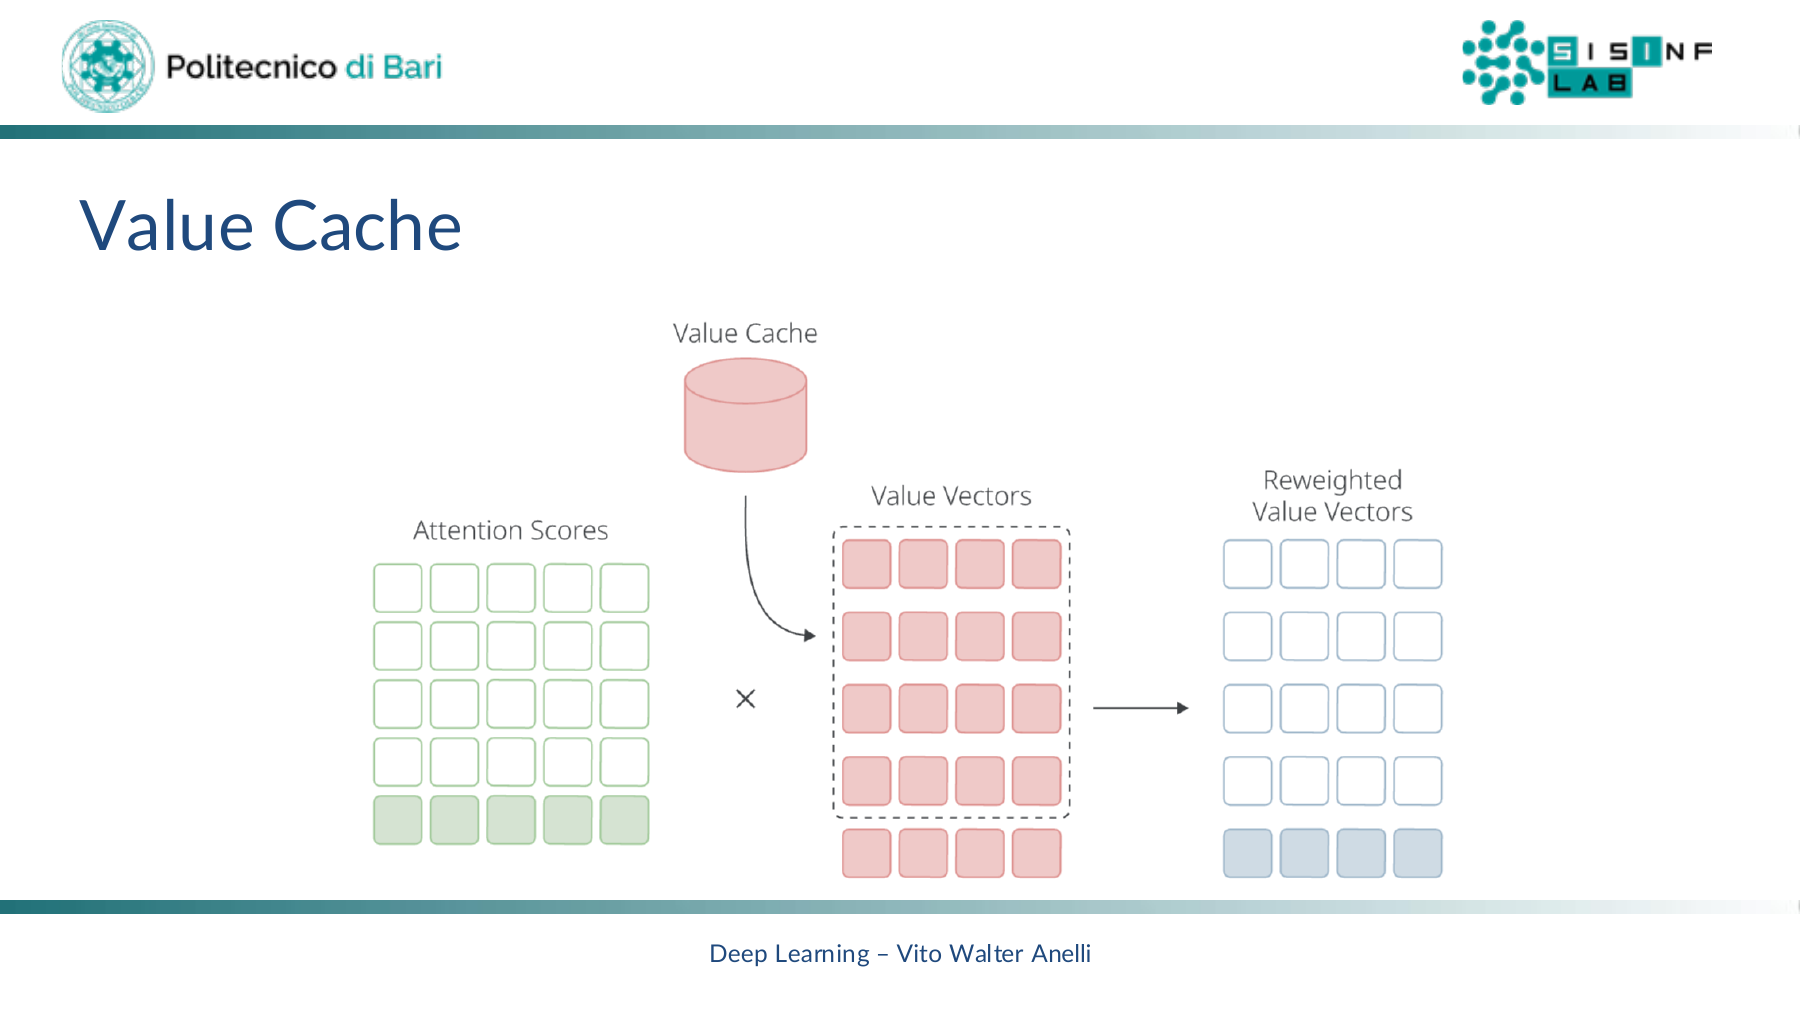
\includegraphics[width=0.80\linewidth]{figures/cf17_value_cache.png}
  \caption{Meccanismo della Value Cache. I vettori valore dei token precedenti
           sono recuperati dalla cache e usati nella somma pesata tramite
           i punteggi di attenzione del token corrente.}
  \label{fig:value-cache}
\end{figure}

\subsection{Dimensione della KV Cache}
\label{subsec:kv-cache-size}

La dimensione in memoria della KV Cache si determina considerando i seguenti
iper-parametri:

\begin{itemize}
  \item $l$: numero di layer del Transformer,
  \item $b$: batch size,
  \item $n$: numero di attention head,
  \item $h$: dimensione di ciascun head ($d_h$),
  \item $s$: lunghezza della sequenza.
\end{itemize}

Il tensore KV Cache per un singolo layer ha forma $(b,\, n,\, s,\, h)$.
Considerando sia le Key che i Value (fattore $\times 2$) e la
rappresentazione in mezza precisione FP16 ($2$ byte per elemento), la
dimensione totale in byte è:
\begin{equation}
  \text{KV Cache size} = l \times b \times n \times h \times s \times 2 \times 2
  \quad \text{[byte]}.
  \label{eq:kv-cache-size}
\end{equation}
A titolo d'esempio, per GPT-3 (175B parametri) con $b=1$ e $s=1024$, la KV
Cache occupa circa $4.5$ GB, una quantità non trascurabile rispetto alla VRAM
disponibile.

\begin{table}[H]
  \centering
  \caption{Dimensione della KV Cache (MHA standard) per le varianti di GPT-3
           con $b=1$, $s=1024$.}
  \label{tab:kv-cache-size-mha}
  \small
  \begin{tabular}{lrr}
    \toprule
    \textbf{Modello} & \textbf{Parametri} & \textbf{KV Cache} \\
    \midrule
    GPT-3 Small  & 125M  & 36 MB  \\
    GPT-3 Medium & 350M  & 96 MB  \\
    GPT-3 Large  & 760M  & 144 MB \\
    GPT-3 XL     & 1.3B  & 288 MB \\
    GPT-3 2.7B   & 2.7B  & 320 MB \\
    GPT-3 6.7B   & 6.7B  & 512 MB \\
    GPT-3 13B    & 13B   & 800 MB \\
    GPT-3        & 175B  & 4.5 GB \\
    \bottomrule
  \end{tabular}
\end{table}

%------------------------------------------------------------
\section{Multi-Query Attention}
\label{sec:mqa}

\subsection{Motivazione}
\label{subsec:mqa-motivation}

Nella MHA standard ogni head $i$ dispone di proiezioni Key e Value
\emph{indipendenti}: $W_K^{(i)}$ e $W_V^{(i)}$. La KV Cache deve quindi
memorizzare $n$ coppie $(K_i, V_i)$, il che scala linearmente con il numero
di head. La \textbf{Multi-Query Attention} (MQA) \citep{shazeer2019fast},
adottata in modelli come PaLM (Google) e Falcon, riduce questo costo
mantenendo un unico set di proiezioni Key e Value condiviso tra tutti
gli head delle query.

\subsection{Architettura}
\label{subsec:mqa-architecture}

Nella MQA si hanno $n$ proiezioni di query distinte, ma \textbf{una sola}
proiezione di Key e una sola di Value:
\begin{align}
  Q_i &= X W_Q^{(i)}, \quad i = 1,\ldots,n, \\
  K   &= X W_K, \\
  V   &= X W_V,
\end{align}
dove $W_K, W_V \in \mathbb{R}^{d_{\text{model}} \times d_h}$ sono le
proiezioni condivise. Il calcolo dell'attenzione per il head $i$ diventa:
\begin{equation}
  \text{head}_i = \text{Softmax}\!\left(\frac{Q_i K^\top}{\sqrt{d_h}}\right) V.
\end{equation}
Ogni head utilizza la stessa sequenza di chiavi e valori, ma con query
differenti, consentendo specializzazioni diverse nelle rappresentazioni
di output.

\begin{figure}[H]
  \centering
  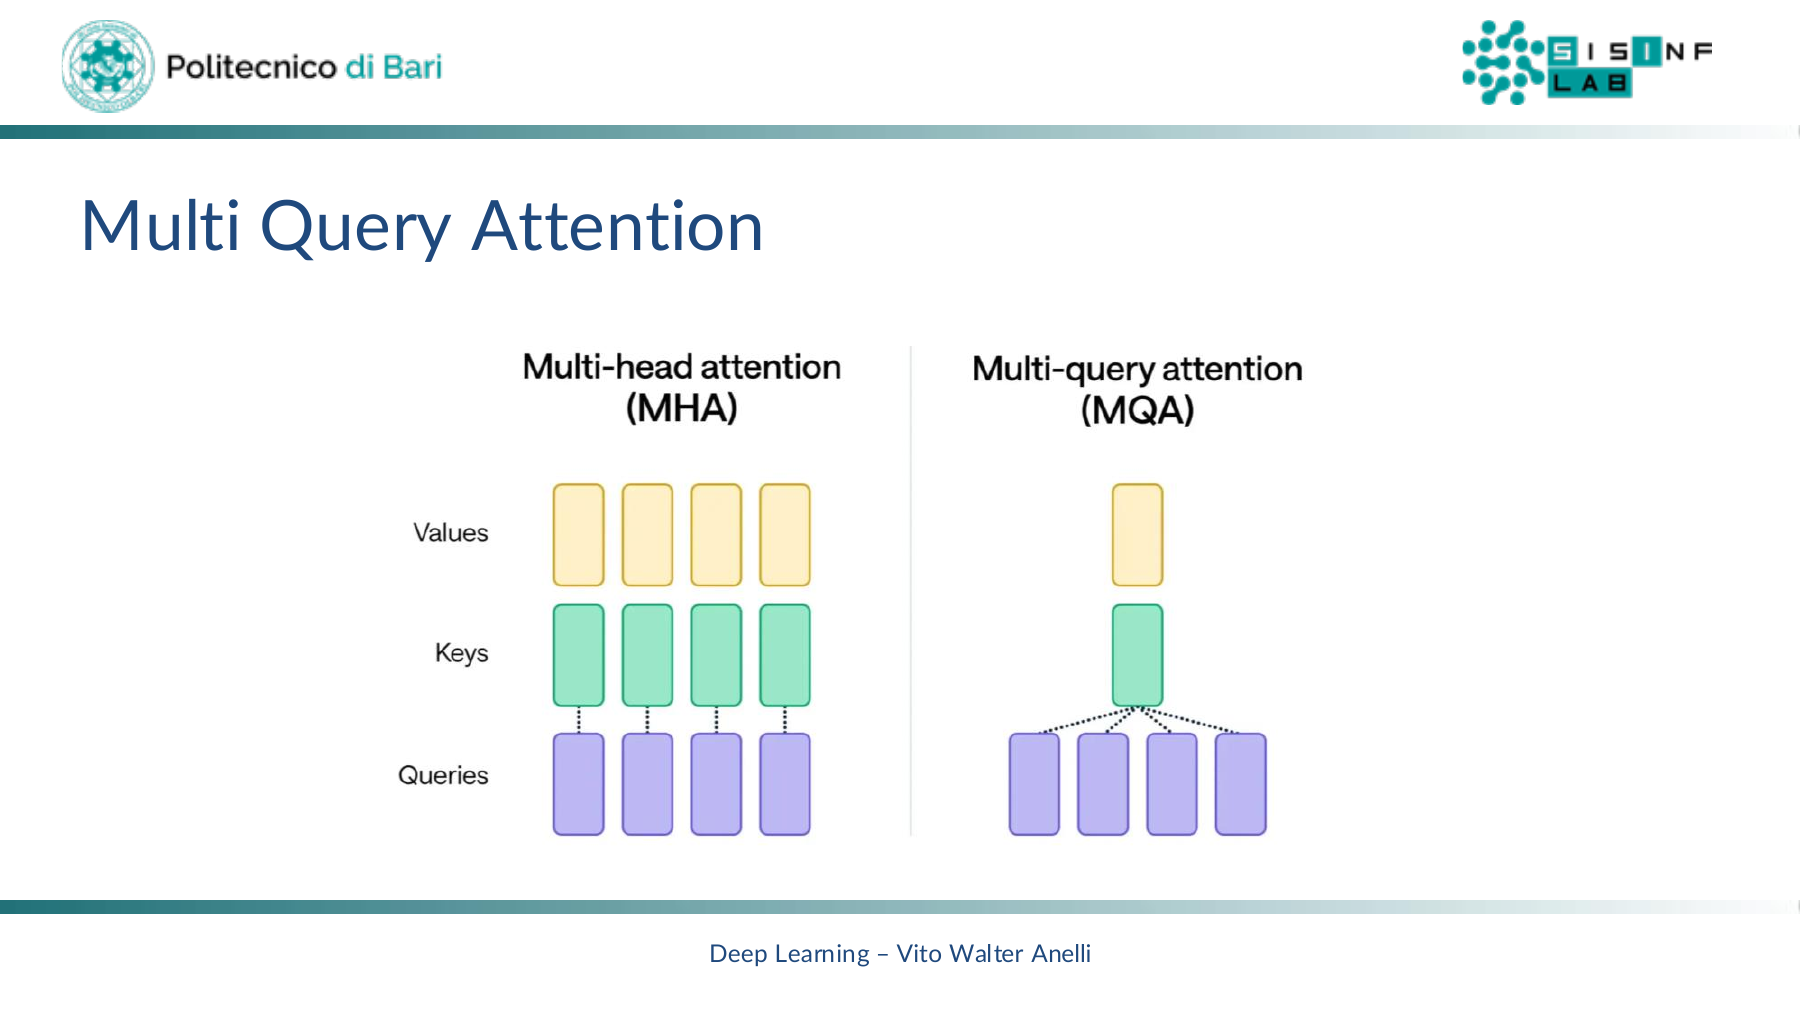
\includegraphics[width=0.72\linewidth]{figures/cf17_mha_vs_mqa.png}
  \caption{Confronto tra Multi-Head Attention (MHA) e Multi-Query Attention
           (MQA). In MHA ogni head possiede Key, Value e Query indipendenti.
           In MQA tutti gli head condividono un unico set di Key e Value,
           mentre le Query rimangono distinte.}
  \label{fig:mha-vs-mqa}
\end{figure}

\subsection{Dimensione della KV Cache con MQA}
\label{subsec:mqa-kv-cache}

Poiché Key e Value sono condivisi tra tutti gli $n$ head, la KV Cache
si riduce di un fattore $n$. La dimensione della cache con MQA è:
\begin{equation}
  \text{KV Cache size (MQA)} = l \times b \times s \times h \times 2 \times 2
  \quad \text{[byte]},
  \label{eq:kv-cache-size-mqa}
\end{equation}
che corrisponde esattamente all'equazione~\eqref{eq:kv-cache-size} senza
il fattore $n$. Il risparmio è quindi pari a $n$ volte rispetto alla MHA.

\begin{table}[H]
  \centering
  \caption{Confronto della dimensione della KV Cache tra MHA e MQA per le
           varianti di GPT-3, con $b=1$, $s=1024$.}
  \label{tab:kv-cache-mha-vs-mqa}
  \small
  \begin{tabular}{lrrr}
    \toprule
    \textbf{Modello} & \textbf{Parametri} & \textbf{KV Cache (MHA)} & \textbf{KV Cache (MQA)} \\
    \midrule
    GPT-3 Small  & 125M  & 36 MB   & 3 MB   \\
    GPT-3 Medium & 350M  & 96 MB   & 6 MB   \\
    GPT-3 Large  & 760M  & 144 MB  & 9 MB   \\
    GPT-3 XL     & 1.3B  & 288 MB  & 12 MB  \\
    GPT-3 2.7B   & 2.7B  & 320 MB  & 10 MB  \\
    GPT-3 6.7B   & 6.7B  & 512 MB  & 16 MB  \\
    GPT-3 13B    & 13B   & 800 MB  & 20 MB  \\
    GPT-3        & 175B  & 4.5 GB  & 48 MB  \\
    \bottomrule
  \end{tabular}
\end{table}

\subsection{Impatto sulle Prestazioni}
\label{subsec:mqa-performance}

La MQA introduce un leggero degrado qualitativo rispetto alla MHA, poiché
riduce la capacità espressiva dei Key e Value. Tuttavia, le valutazioni
empiriche su T5-XXL (Rouge score su CNN, arXiv, PubMed, MultiNews) e LLaMA~2
(zero-shot accuracy su BoolQ, PIQA, Hella-Swag, ARC-Easy) mostrano che il
degrado è contenuto, dell'ordine di 1--2 punti percentuali, a fronte di
un risparmio di memoria di un ordine di grandezza \citep{shazeer2019fast}.

%------------------------------------------------------------
\section{Grouped-Query Attention}
\label{sec:gqa}

\subsection{Motivazione e Architettura}
\label{subsec:gqa-architecture}

La \textbf{Grouped-Query Attention} (GQA) \citep{ainslie2023gqa}, adottata
in LLaMA~2, LLaMA~3 e Mistral 7B, rappresenta un compromesso continuo tra
MHA e MQA. Gli $n$ head di query vengono suddivisi in $G$ gruppi ($G$
divisore di $n$), dove ogni gruppo condivide un unico set di Key e Value.
Con $G = 1$ si recupera la MQA; con $G = n$ si recupera la MHA.

Definendo $n_g = n / G$ il numero di query head per gruppo, le proiezioni sono:
\begin{align}
  Q_i     &= X W_Q^{(i)}, \quad i = 1,\ldots,n, \\
  K_{[g]} &= X W_K^{(g)}, \quad g = 1,\ldots,G, \\
  V_{[g]} &= X W_V^{(g)}, \quad g = 1,\ldots,G.
\end{align}
Il head $i$, appartenente al gruppo $g(i) = \lceil i\,n/G \rceil$, calcola:
\begin{equation}
  \text{head}_i = \text{Softmax}\!\left(
    \frac{Q_i K_{[g(i)]}^\top}{\sqrt{d_h}}
  \right) V_{[g(i)]}.
\end{equation}

\begin{figure}[H]
  \centering
  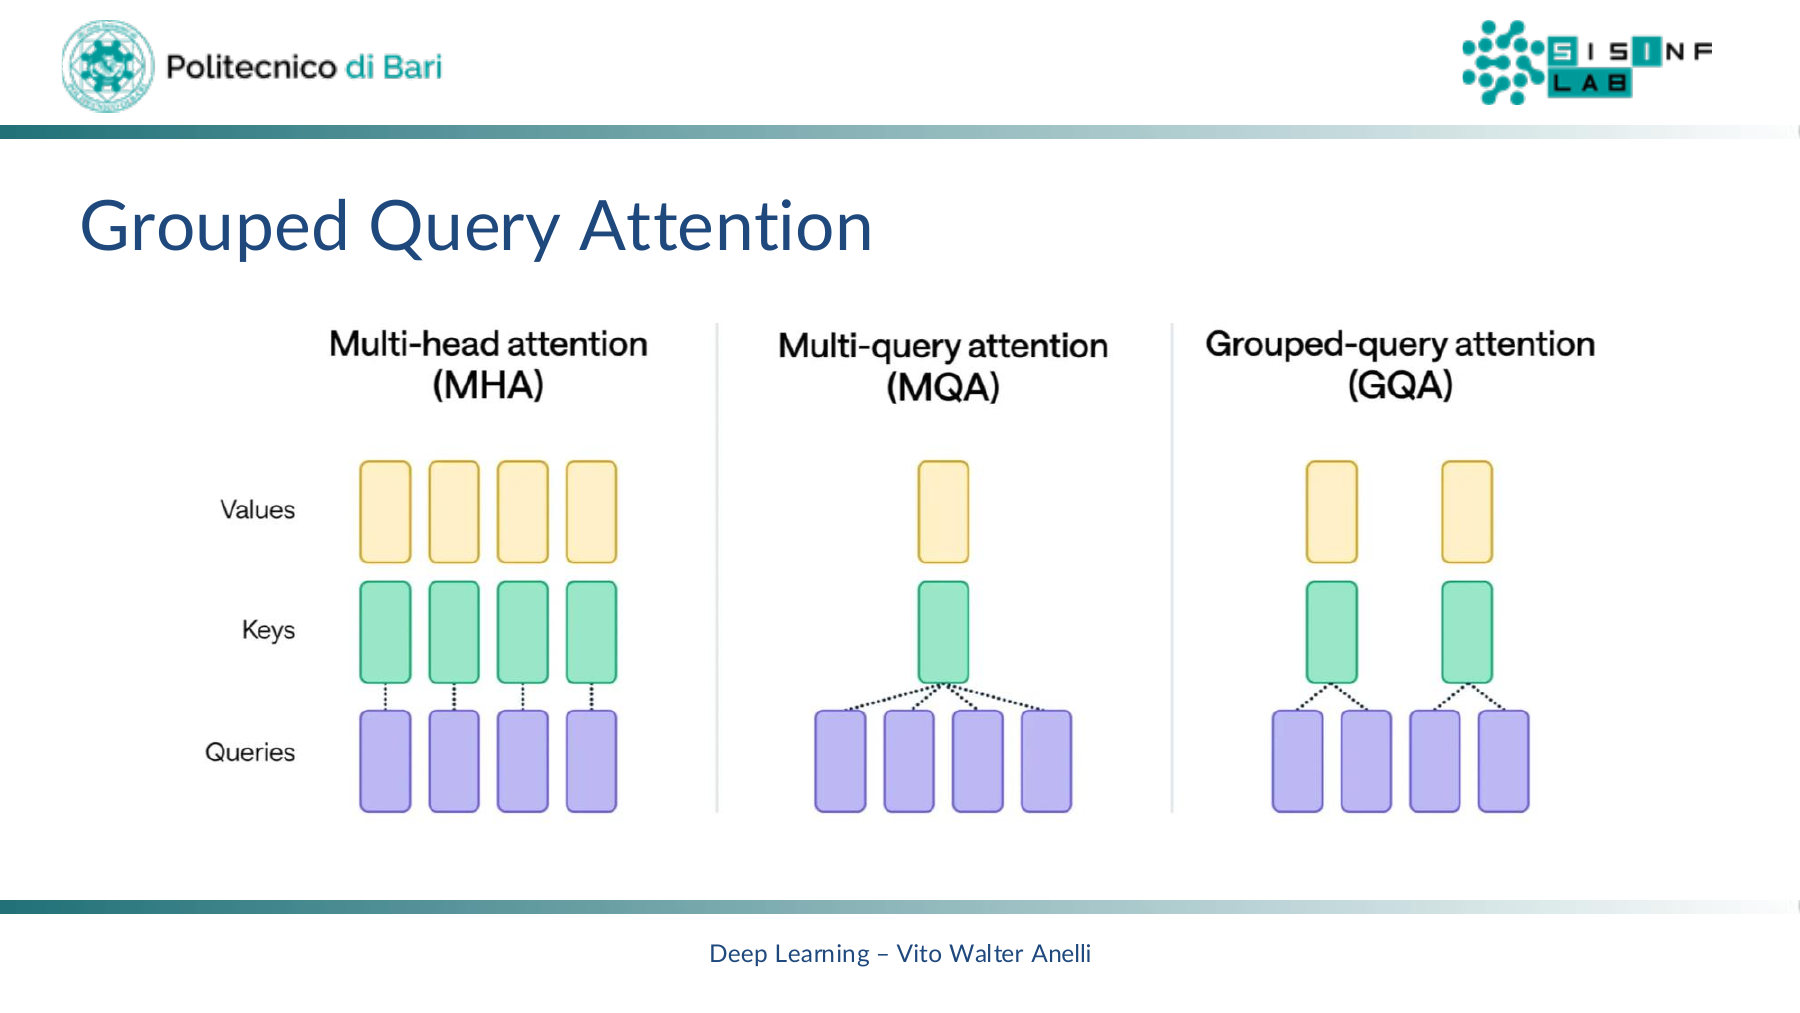
\includegraphics[width=0.85\linewidth]{figures/cf17_mha_mqa_gqa.png}
  \caption{Confronto tra MHA, MQA e GQA. In GQA gli $n$ head di query sono
           divisi in $G$ gruppi, ognuno con le proprie Key e Value condivise
           tra i membri del gruppo. Con $G=n$ si ottiene MHA, con $G=1$
           si ottiene MQA.}
  \label{fig:gqa}
\end{figure}

\subsection{Dimensione della KV Cache con GQA}
\label{subsec:gqa-kv-cache}

La KV Cache con GQA scala con il numero di gruppi $G$:
\begin{equation}
  \text{KV Cache size (GQA)} = l \times b \times G \times h \times s \times 2 \times 2
  \quad \text{[byte]}.
  \label{eq:kv-cache-size-gqa}
\end{equation}
Il risparmio rispetto alla MHA è pari a $n/G$: con $G=8$ e $n=32$ si ottiene
un fattore $4\times$ di riduzione, con un degrado qualitativo inferiore
rispetto alla MQA.

\subsection{Impatto sulle Prestazioni}
\label{subsec:gqa-performance}

La GQA con $G=8$ su T5-XXL raggiunge prestazioni molto vicine alla MHA
(entro 0.5 punti Rouge), superando la MQA in tutti i benchmark considerati.
Questo rende la GQA la scelta preferita nei modelli di grandi dimensioni
moderni, in quanto offre un ottimo compromesso tra efficienza della memoria
e capacità del modello \citep{ainslie2023gqa}.

%------------------------------------------------------------
\section{Rotary Positional Embeddings (RoPE)}
\label{sec:rope}

\subsection{Limiti degli Embedding Posizionali Assoluti}
\label{subsec:absolute-pe-limits}

Gli embedding posizionali assoluti (come quelli originali del Transformer
\citep{vaswani2017attention}) assegnano a ciascuna posizione $m$ un vettore
fisso $\mathbf{p}_m$, sommato all'embedding del token prima dell'attenzione.
Questa formulazione presenta due limiti fondamentali:

\begin{itemize}
  \item \textbf{Lunghezza massima fissa}: il modello non può rappresentare
        posizioni oltre la lunghezza massima vista durante il training.
  \item \textbf{Indipendenza posizionale}: ogni embedding è indipendente
        dagli altri. Il modello tratta la differenza tra le posizioni $1$ e $2$
        allo stesso modo della differenza tra le posizioni $2$ e $500$,
        ostacolando la comprensione della struttura relativa della sequenza.
\end{itemize}

\subsection{Embedding Posizionali Relativi}
\label{subsec:relative-pe}

Gli embedding posizionali relativi (ad esempio in T5 \citep{raffel2020t5})
modellano la \emph{distanza} tra coppie di token anziché la loro posizione
assoluta. In T5, un bias scalare $b(m-n)$ viene aggiunto alla matrice di
attenzione $Q K^\top$ tra il token in posizione $m$ e quello in posizione $n$:
\begin{equation}
  A_{mn} \leftarrow \frac{\mathbf{q}_m \cdot \mathbf{k}_n}{\sqrt{d_h}} + b(m-n).
\end{equation}
Sebbene concettualmente più ricchi, gli embedding relativi presentano
problemi pratici:
\begin{itemize}
  \item Maggiore costo computazionale, specialmente per sequenze lunghe.
  \item \textbf{Incompatibilità con la KV Cache}: aggiungere un nuovo token
        modifica l'embedding relativo di tutti i token precedenti,
        invalidando la cache.
\end{itemize}
Per questi motivi, gli embedding relativi non hanno trovato ampia adozione
nei grandi modelli linguistici.

\subsection{Matrice di Rotazione}
\label{subsec:rotation-matrix}

Alla base di RoPE vi è la \textbf{matrice di rotazione 2D}, che ruota un
vettore di un angolo $\theta$ preservandone la norma:
\begin{equation}
  R(\theta) = \begin{pmatrix} \cos\theta & -\sin\theta \\ \sin\theta & \cos\theta \end{pmatrix},
  \qquad
  R(\theta)\,\mathbf{x} = \begin{pmatrix} \cos\theta\, x_1 - \sin\theta\, x_2 \\
                                            \sin\theta\, x_1 + \cos\theta\, x_2 \end{pmatrix}.
  \label{eq:rotation-matrix}
\end{equation}
La moltiplicazione per $R(\theta)$ cambia la direzione del vettore senza
alterarne la lunghezza. Questa proprietà è fondamentale per costruire
embedding posizionali che si comportino bene nel prodotto scalare.

\subsection{Formulazione di RoPE}
\label{subsec:rope-formulation}

I \textbf{Rotary Positional Embeddings} (RoPE) \citep{su2024rope}, adottati in
RoFormer, LLaMA~2/3, Gemma, PaLM, GPT-NeoX, Falcon e DeepSeek, incorporano
l'informazione posizionale \emph{all'interno} del calcolo del prodotto
scalare tra query e key, anziché aggiungerla agli embedding di input.

Per un vettore di query o key a $d_h$ dimensioni nella posizione $m$, RoPE
applica una rotazione dipendente dalla posizione. Nel caso 2D, la query
$\mathbf{q} = W_Q \mathbf{x}$ viene trasformata come:
\begin{equation}
  \text{RoPE}(\mathbf{q}, m) = R(m\theta)\, W_Q\, \mathbf{x}
  = \begin{pmatrix} \cos m\theta & -\sin m\theta \\
                    \sin m\theta & \phantom{-}\cos m\theta \end{pmatrix}
    W_Q \begin{pmatrix} x_1 \\ x_2 \end{pmatrix}.
  \label{eq:rope-query}
\end{equation}
Analogamente, la key in posizione $n$ viene trasformata con $R(n\theta)$.

Le rotazioni godono della seguente proprietà algebrica:

\begin{theorem}[Prodotto tra rotazioni]
Per qualsiasi angolo $\alpha, \beta$:
\begin{equation}
  R(\alpha)^\top R(\beta) = R(\beta - \alpha).
  \label{eq:rotation-product}
\end{equation}
\end{theorem}

Applicando questo risultato al calcolo del punteggio di attenzione tra i
token in posizione $m$ e $n$:
\begin{align}
  \text{score}(m, n)
    &= \mathbf{q}_m^\top \mathbf{k}_n \notag \\
    &= \bigl(R(m\theta)\,\mathbf{q}\bigr)^\top \bigl(R(n\theta)\,\mathbf{k}\bigr) \notag \\
    &= \mathbf{q}^\top R(m\theta)^\top R(n\theta)\,\mathbf{k} \notag \\
    &= \mathbf{q}^\top R\bigl((n-m)\theta\bigr)\,\mathbf{k}.
  \label{eq:rope-score}
\end{align}
Il punteggio di attenzione dipende quindi solo dalla \textbf{distanza
relativa} $n - m$ tra i due token, non dalle posizioni assolute. Questo
garantisce la proprietà degli embedding relativi, pur essendo applicato
localmente alle singole coppie (query, key).

\begin{figure}[H]
  \centering
  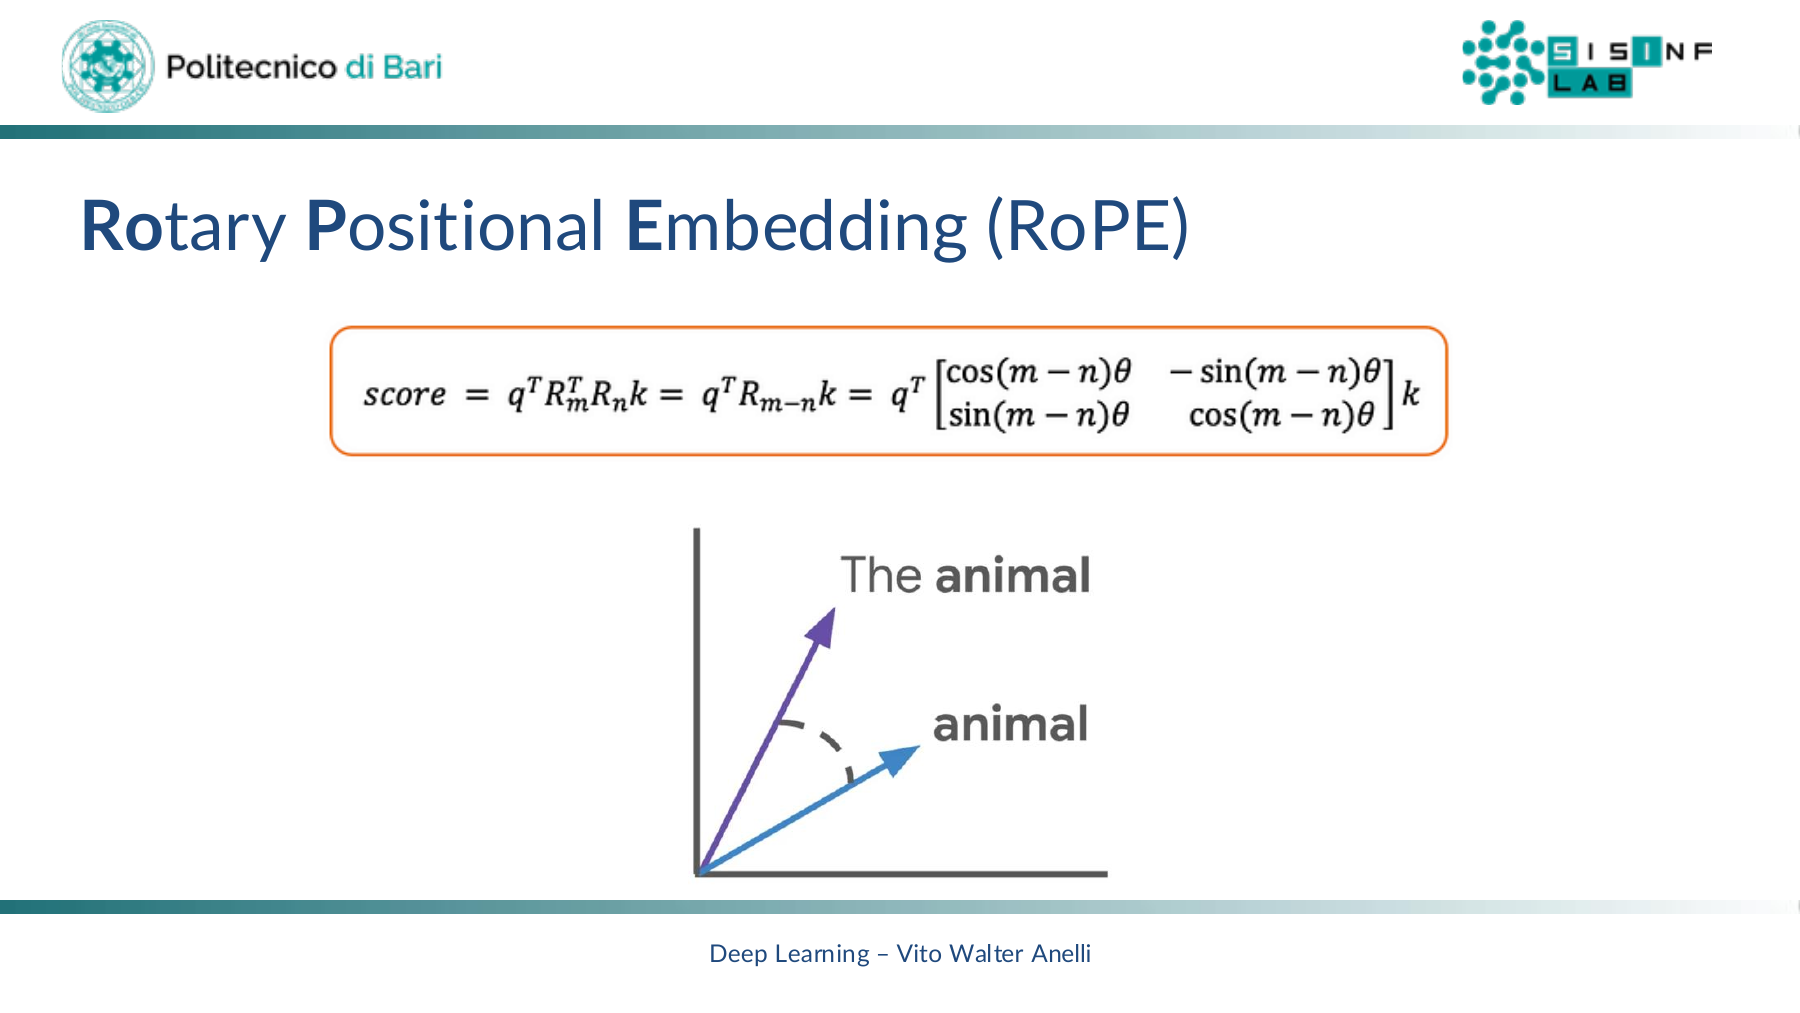
\includegraphics[width=0.62\linewidth]{figures/cf17_rope_score.png}
  \caption{Interpretazione geometrica di RoPE. La parola \emph{animal}
           appare in due posizioni diverse nella sequenza; RoPE la rappresenta
           come due vettori ruotati di angoli diversi. Il prodotto scalare
           tra la query e la key cattura la distanza relativa tra le due
           occorrenze.}
  \label{fig:rope-score}
\end{figure}

\subsection{Estensione a dimensioni superiori}
\label{subsec:rope-higher-dim}

In pratica $d_h > 2$. RoPE estende la formulazione 2D suddividendo il
vettore di query (o key) in $d_h/2$ coppie di dimensioni, applicando
a ciascuna coppia $(x_{2i-1}, x_{2i})$ una rotazione di angolo $m\theta_i$,
con frequenze geometricamente spaziate:
\begin{equation}
  \theta_i = \theta_{\text{base}}^{-2(i-1)/d_h},
  \qquad \theta_{\text{base}} = 10000 \text{ (default)}.
  \label{eq:rope-freq}
\end{equation}
Le basse frequenze catturano strutture di lungo raggio, le alte frequenze
strutture locali, in modo analogo agli embedding sinusoidali originali di
\citet{vaswani2017attention} ma con la proprietà aggiuntiva di essere
compatibili con la KV Cache.

\paragraph{Compatibilità con la KV Cache.}
Poiché RoPE agisce localmente sui vettori query e key (anziché sugli
embedding di input), i vettori chiave già memorizzati nella cache rimangono
validi: è sufficiente applicare la rotazione $R(m\theta)$ alla key del
nuovo token prima di inserirla in cache.

%------------------------------------------------------------
\section{Multi-Head Latent Attention}
\label{sec:mla}

\subsection{Motivazione}
\label{subsec:mla-motivation}

La \textbf{Multi-Head Latent Attention} (MLA) \citep{deepseekv2_2024},
introdotta in DeepSeek V2/V3/R1, propone un'alternativa radicalmente diversa
a MQA e GQA per ridurre la KV Cache. Invece di ridurre il numero di head
per Key e Value, MLA \textbf{comprime} l'intera rappresentazione KV in un
vettore latente di bassa dimensione, che viene poi espanso quando serve.

\subsection{Compressione della KV Cache}
\label{subsec:mla-compression}

Dato il vettore di input $\mathbf{h}_t \in \mathbb{R}^{d}$ al passo $t$
(dove $d = n_h \cdot d_h$ è la dimensione del modello), la proiezione
\emph{down-projection} comprime $\mathbf{h}_t$ in un vettore latente di
dimensione $d_c \ll d$:
\begin{equation}
  \mathbf{c}_t^{KV} = W^{DKV} \mathbf{h}_t,
  \qquad W^{DKV} \in \mathbb{R}^{d_c \times d}.
  \label{eq:mla-compress}
\end{equation}
Quando è necessario calcolare l'attenzione, Key e Value vengono recuperati
tramite le proiezioni \emph{up-projection}:
\begin{equation}
  \mathbf{k}_t^C = W^{UK} \mathbf{c}_t^{KV},
  \qquad
  \mathbf{v}_t^C = W^{UV} \mathbf{c}_t^{KV},
  \label{eq:mla-up-kv}
\end{equation}
dove $W^{UK}, W^{UV} \in \mathbb{R}^{(n_h d_h) \times d_c}$ sono le
matrici di espansione. Nella cache viene memorizzato \textbf{solo}
$\mathbf{c}_t^{KV}$, non le Key e Value espanse.

Analogamente, anche le query vengono compresse e poi espanse:
\begin{equation}
  \mathbf{c}_t^Q = W^{DQ} \mathbf{h}_t, \qquad
  \mathbf{q}_t^C = W^{UQ} \mathbf{c}_t^Q.
  \label{eq:mla-query}
\end{equation}

\begin{figure}[H]
  \centering
  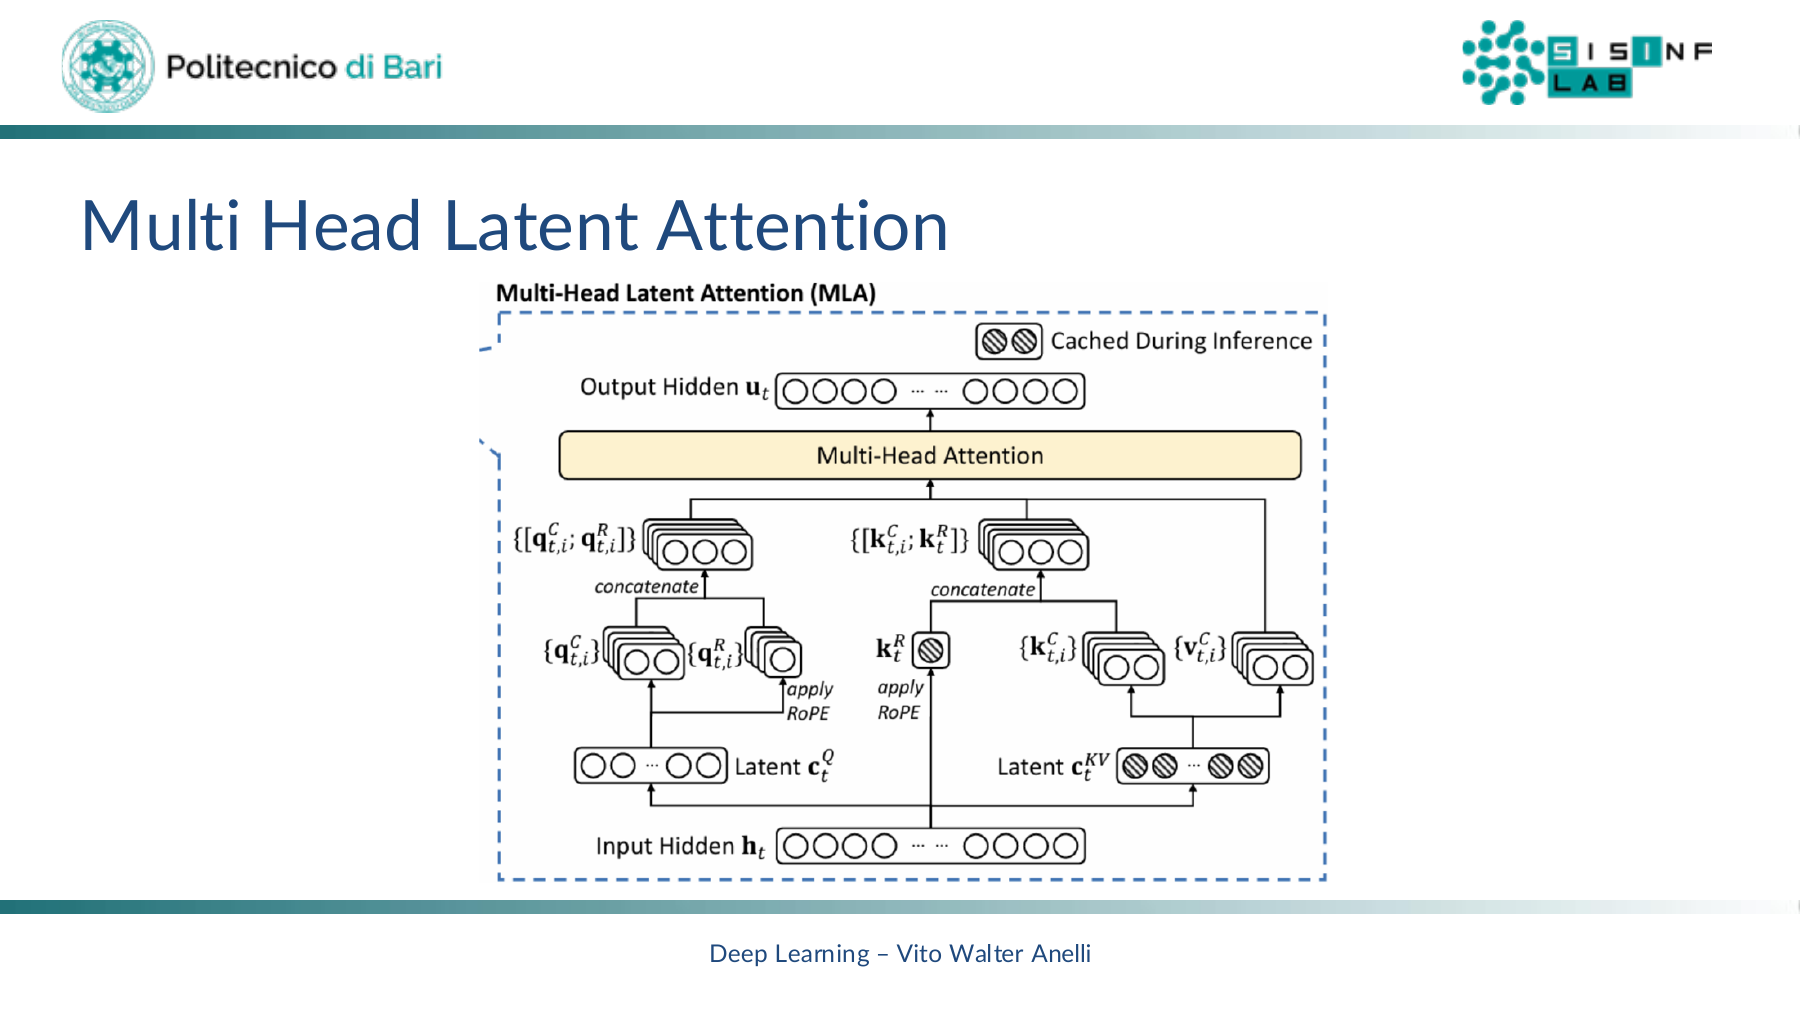
\includegraphics[width=0.85\linewidth]{figures/cf17_mla_architecture.png}
  \caption{Schema completo della Multi-Head Latent Attention (MLA). Il
           vettore di input $\mathbf{h}_t$ viene proiettato in due vettori
           latenti $\mathbf{c}_t^Q$ e $\mathbf{c}_t^{KV}$ (dimensione
           ridotta). Solo $\mathbf{c}_t^{KV}$ viene memorizzato in cache.
           Le query, le key e i value vengono ricostruiti tramite
           up-projection prima del calcolo dell'attenzione. Le chiavi RoPE
           sono calcolate separatamente e concatenate (decoupled RoPE).}
  \label{fig:mla-architecture}
\end{figure}

\subsection{Assorbimento delle matrici di proiezione}
\label{subsec:mla-absorption}

Un'osservazione chiave è che, nel calcolo del punteggio di attenzione tra
$\mathbf{q}_t^C$ e $\mathbf{k}_t^C$, le matrici $W^{UQ}$ e $W^{UK}$
compaiono sempre insieme:
\begin{equation}
  \mathbf{q}_t^{C\top} \mathbf{k}_t^C
  = \mathbf{c}_t^{Q\top}\bigl(W^{UQ}\bigr)^\top W^{UK} \mathbf{c}_t^{KV}.
\end{equation}
Il prodotto $\bigl(W^{UQ}\bigr)^\top W^{UK}$ può essere precalcolato e
``assorbito'' in $W^{UQ}$, riducendo ulteriormente il numero di parametri
da mantenere in memoria durante l'inferenza.

\subsection{RoPE Disaccoppiata}
\label{subsec:decoupled-rope}

L'applicazione diretta di RoPE alle key compresse è \textbf{incompatibile}
con la strategia di assorbimento: la matrice di rotazione $R(m\theta)$
dipende dalla posizione e non può essere assorbita in $W^{UQ}$ (verrebbe
inserita tra i due fattori della moltiplicazione, impedendo la fusione).

La soluzione proposta in \citet{deepseekv2_2024} è il \textbf{RoPE
disaccoppiato}: si introducono vettori di query e key ausiliari
$\mathbf{q}_t^R$ e $\mathbf{k}_t^R$, dedicati esclusivamente alla
codifica posizionale tramite RoPE:
\begin{align}
  \mathbf{q}_t^R &= \text{RoPE}(W^{QR} \mathbf{c}_t^Q, \; t), \\
  \mathbf{k}_t^R &= \text{RoPE}(W^{KR} \mathbf{h}_t, \; t).
\end{align}
Il key condiviso $\mathbf{k}_t^R$ è un singolo vettore per tutte le head
(come in MQA), e viene anch'esso memorizzato in cache. La query e la key
finali sono formate per concatenazione:
\begin{align}
  \mathbf{q}_{t,i} &= [\mathbf{q}_{t,i}^C;\, \mathbf{q}_{t,i}^R], \\
  \mathbf{k}_{t,i} &= [\mathbf{k}_{t,i}^C;\, \mathbf{k}_t^R].
\end{align}

\subsection{Calcolo Completo di MLA}
\label{subsec:mla-computation}

Il calcolo completo di MLA, comprensivo di RoPE disaccoppiata, è il seguente
(Equazioni 37--47 di \citet{deepseekv2_2024}):
\begin{align}
  \mathbf{c}_t^Q &= W^{DQ}\mathbf{h}_t, \tag{37} \\
  [\mathbf{q}_{t,1}^C;\ldots;\mathbf{q}_{t,n_h}^C]
    &= \mathbf{q}_t^C = W^{UQ}\mathbf{c}_t^Q, \tag{38} \\
  [\mathbf{q}_{t,1}^R;\ldots;\mathbf{q}_{t,n_h}^R]
    &= \mathbf{q}_t^R = \text{RoPE}(W^{QR}\mathbf{c}_t^Q), \tag{39} \\
  \mathbf{q}_{t,i} &= [\mathbf{q}_{t,i}^C;\,\mathbf{q}_{t,i}^R], \tag{40} \\[4pt]
  \mathbf{c}_t^{KV} &= W^{DKV}\mathbf{h}_t, \tag{41} \\
  [\mathbf{k}_{t,1}^C;\ldots;\mathbf{k}_{t,n_h}^C]
    &= \mathbf{k}_t^C = W^{UK}\mathbf{c}_t^{KV}, \tag{42} \\
  \mathbf{k}_t^R &= \text{RoPE}(W^{KR}\mathbf{h}_t), \tag{43} \\
  \mathbf{k}_{t,i} &= [\mathbf{k}_{t,i}^C;\,\mathbf{k}_t^R], \tag{44} \\
  [\mathbf{v}_{t,1}^C;\ldots;\mathbf{v}_{t,n_h}^C]
    &= \mathbf{v}_t^C = W^{UV}\mathbf{c}_t^{KV}, \tag{45} \\[4pt]
  \mathbf{o}_{t,i}
    &= \sum_{j=1}^{t} \text{Softmax}_j\!\left(
        \frac{\mathbf{q}_{t,i}^\top \mathbf{k}_{j,i}}{\sqrt{d_h + d_h^R}}
      \right) \mathbf{v}_{j,i}^C, \tag{46} \\
  \mathbf{u}_t &= W^O\,[\mathbf{o}_{t,1};\ldots;\mathbf{o}_{t,n_h}]. \tag{47}
\end{align}

\noindent In cache si memorizzano \textbf{solo} $\mathbf{c}_t^{KV}$ e
$\mathbf{k}_t^R$, ovvero un vettore di dimensione $d_c + d_h^R$ per token per
layer.

\subsection{Dimensione della KV Cache con MLA}
\label{subsec:mla-kv-size}

La tabella seguente confronta la dimensione della KV Cache per token per layer
e la capacità del modello tra i quattro meccanismi di attenzione discussi.

\begin{table}[H]
  \centering
  \caption{Confronto della KV Cache per token per layer e della capacità del
           modello tra le varianti di attention (da \citet{deepseekv2_2024}).
           $n_h$: numero di head; $d_h$: dimensione del head; $n_g$: numero
           di gruppi GQA; $d_c$: dimensione latente MLA; $d_h^R$: dimensione
           della componente RoPE.}
  \label{tab:attention-comparison}
  \small
  \begin{tabular}{lccc}
    \toprule
    \textbf{Meccanismo} & \textbf{KV Cache per token} & \textbf{Capacità} \\
    \midrule
    Multi-Head Attention (MHA)   & $2 n_h d_h l$              & Forte    \\
    Grouped-Query Attention (GQA) & $2 n_g d_h l$             & Moderata \\
    Multi-Query Attention (MQA)  & $2 d_h l$                  & Debole   \\
    \midrule
    MLA (DeepSeek)               & $(d_c + d_h^R)\,l \approx \tfrac{9}{2} d_h l$ & Più forte \\
    \bottomrule
  \end{tabular}
\end{table}

\noindent Nonostante la KV Cache di MLA sia paragonabile a quella di GQA con
un numero ridotto di gruppi, i benchmark su modelli Dense~7B e MoE mostrano
che MLA supera MHA sia in qualità (BBH, MMLU, C-Eval, CMMLU) sia in efficienza
di memoria, grazie alla ricchezza semantica del vettore latente compresso
\citep{deepseekv2_2024}.

%------------------------------------------------------------
\section{Riepilogo e Confronto}
\label{sec:attention-summary}

\begin{table}[H]
  \centering
  \caption{Riepilogo delle varianti di Multi-Head Attention. $n$: numero di
           head; $G$: numero di gruppi GQA; $d_c$: dimensione latente MLA.}
  \label{tab:attention-summary}
  \small
  \begin{tabular}{lcccc}
    \toprule
    \textbf{Meccanismo} & \textbf{Key/Value head} & \textbf{KV Cache} & \textbf{Qualità} & \textbf{Adottato in} \\
    \midrule
    MHA  & $n$ indipendenti  & $O(n)$     & Massima  & GPT, BERT \\
    MQA  & 1 condiviso       & $O(1)$     & Ridotta  & PaLM, Falcon \\
    GQA  & $G$ condivisi     & $O(G)$     & Alta     & LLaMA 2/3, Mistral \\
    MLA  & Vettore latente   & $O(d_c/d)$ & Massima+ & DeepSeek V2/V3/R1 \\
    \bottomrule
  \end{tabular}
\end{table}

\paragraph{Osservazione sull'embedding posizionale.}
Le tecniche MHA, MQA e GQA sono agnostiche rispetto alla codifica
posizionale. RoPE è invece un'alternativa agli embedding assoluti e
relativi che risulta \textbf{compatibile con la KV Cache}, poiché la
rotazione posizionale può essere applicata localmente al momento
dell'inserimento del nuovo token. La combinazione GQA + RoPE è attualmente
la scelta architetturale dominante nei modelli \emph{open-weight} di grandi
dimensioni (LLaMA~3, Mistral, Gemma), mentre MLA + RoPE disaccoppiata è
la scelta di DeepSeek per massimizzare sia la qualità che l'efficienza
\citep{deepseekv2_2024,ainslie2023gqa,su2024rope}.



% --- aggiungere qui i prossimi capitoli ---
% %============================================================
%  Capitolo 2 – Learning Representations
%============================================================
\chapter{Learning Representations}
\label{ch:learning-repr}

Questo capitolo affronta una domanda fondamentale: \textit{perché le reti profonde
funzionano meglio di quelle shallow?} La risposta passa per il concetto di
\textbf{rappresentazione}: trasformare i dati grezzi in uno spazio in cui il
problema diventi più facile da risolvere \citep{bishop2024, lecun2021}.

%------------------------------------------------------------
\section{Limiti dei Classificatori Lineari}
\label{sec:linear-limits}

Un \textbf{classificatore lineare} assegna la classe in base al segno di una
combinazione lineare delle feature:
\begin{equation}
  \bar{y} = \operatorname{sign}\!\left(\sum_{i=1}^{N} w_i x_i + b\right).
\end{equation}
Geometricamente, il classificatore partiziona lo spazio in due semispazi
separati dall'iperpiano $\sum_i w_i x_i + b = 0$. Il vettore $\vect{w}$
è la normale all'iperpiano e ne determina l'orientamento; $-b/w_1$ ne fissa
l'intercetta.

\begin{figure}[H]
  \centering
  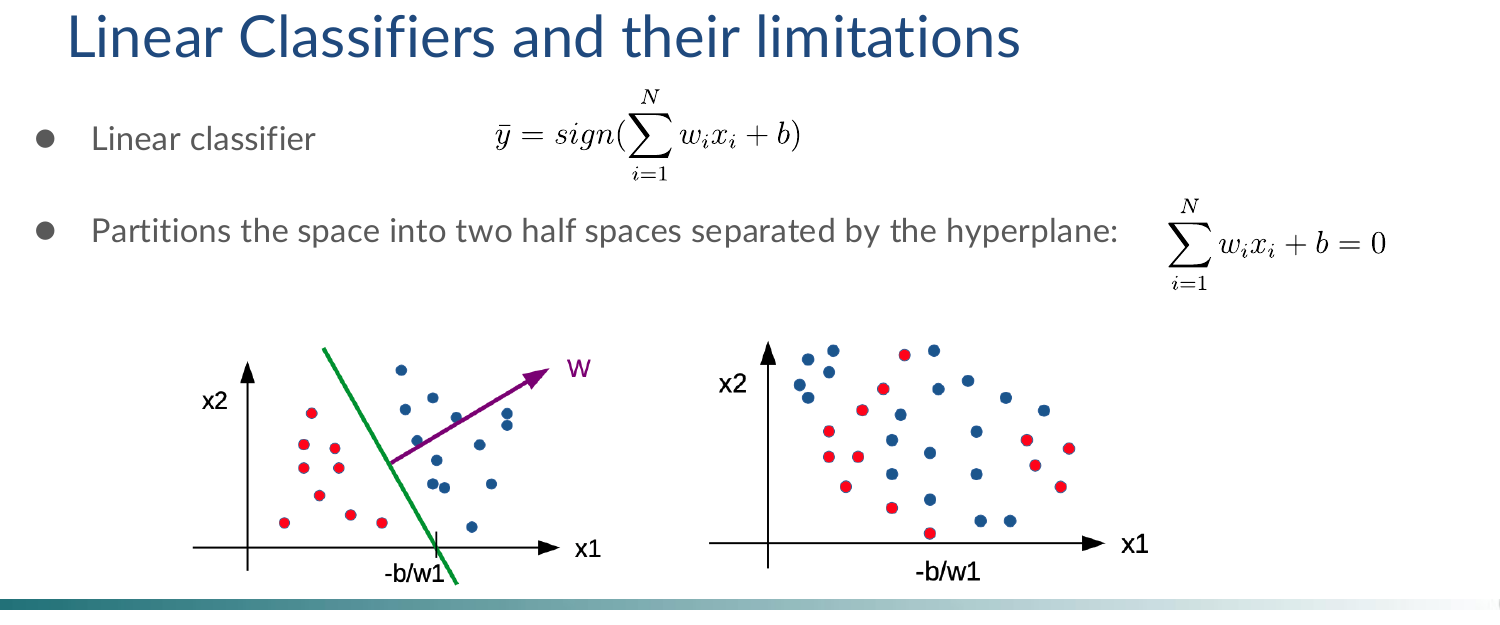
\includegraphics[width=0.88\linewidth]{figures/lr02_linear_classifier.png}
  \caption{Classificatore lineare in 2D. Sinistra: caso separabile linearmente
           -- l'iperpiano (retta verde) divide correttamente le due classi.
           Destra: caso non separabile linearmente -- nessuna retta può separare
           i punti rossi da quelli blu.}
  \label{fig:linear_classifier}
\end{figure}

Il limite fondamentale dei classificatori lineari è formalizzato dal
\textbf{Teorema di Cover (1966)}: la probabilità che una dicotomia casuale
di $P$ punti in $N$ dimensioni sia linearmente separabile tende a zero
quando $P \gg N$.

\begin{figure}[H]
  \centering
  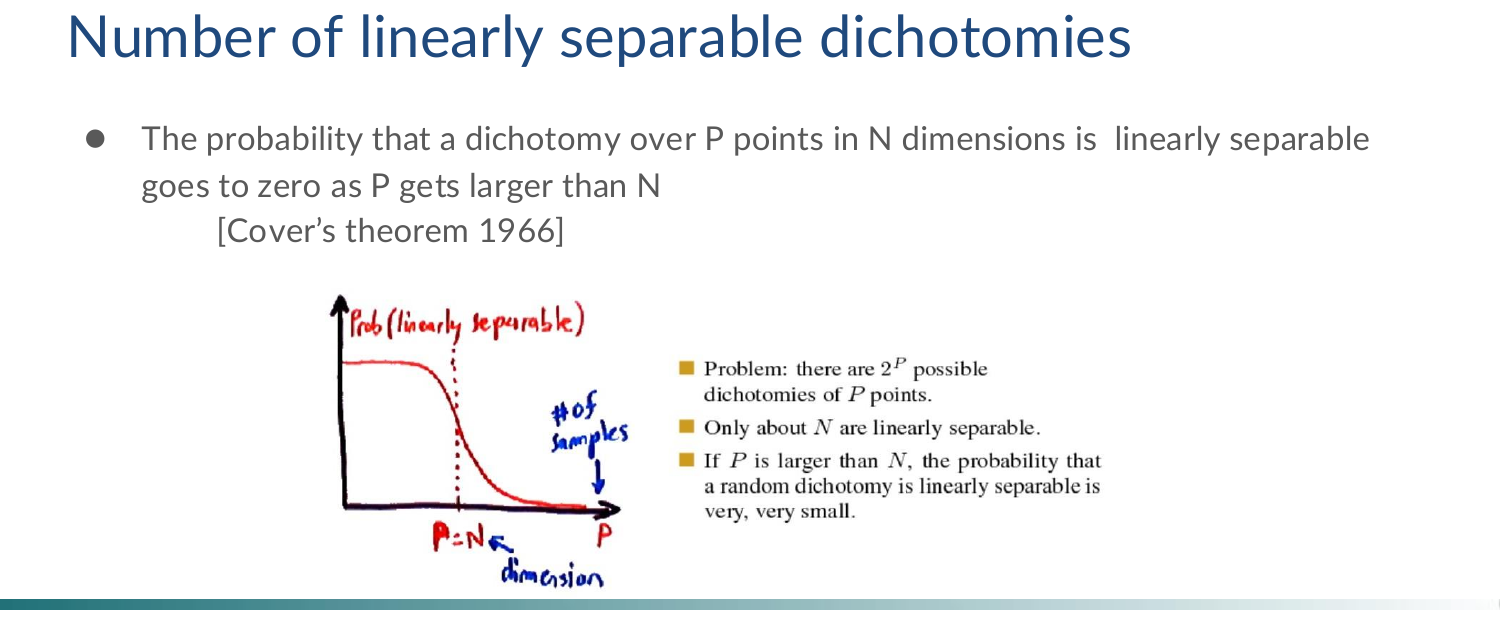
\includegraphics[width=0.75\linewidth]{figures/lr02_cover_theorem.png}
  \caption{Teorema di Cover: la probabilità di separabilità lineare crolla
           bruscamente non appena il numero di campioni $P$ supera la
           dimensionalità $N$. Esistono $2^P$ possibili dicotomie, ma solo
           circa $N$ sono linearmente separabili.}
  \label{fig:cover_theorem}
\end{figure}

In pratica: con $P \gg N$, quasi nessuna dicotomia casuale è linearmente
separabile. Per classificare dati reali complessi, occorre una
\textbf{trasformazione non lineare} che renda il problema separabile.

%------------------------------------------------------------
\section{La Soluzione: Rappresentazioni (Feature)}
\label{sec:solution-repr}

La soluzione è costruire un \textbf{estrattore di feature} che trasformi
l'input grezzo in una rappresentazione in cui un classificatore lineare
possa operare efficacemente. L'estrattore deve essere \emph{non lineare}:
una trasformazione lineare non cambia la separabilità del problema.

\begin{figure}[H]
  \centering
  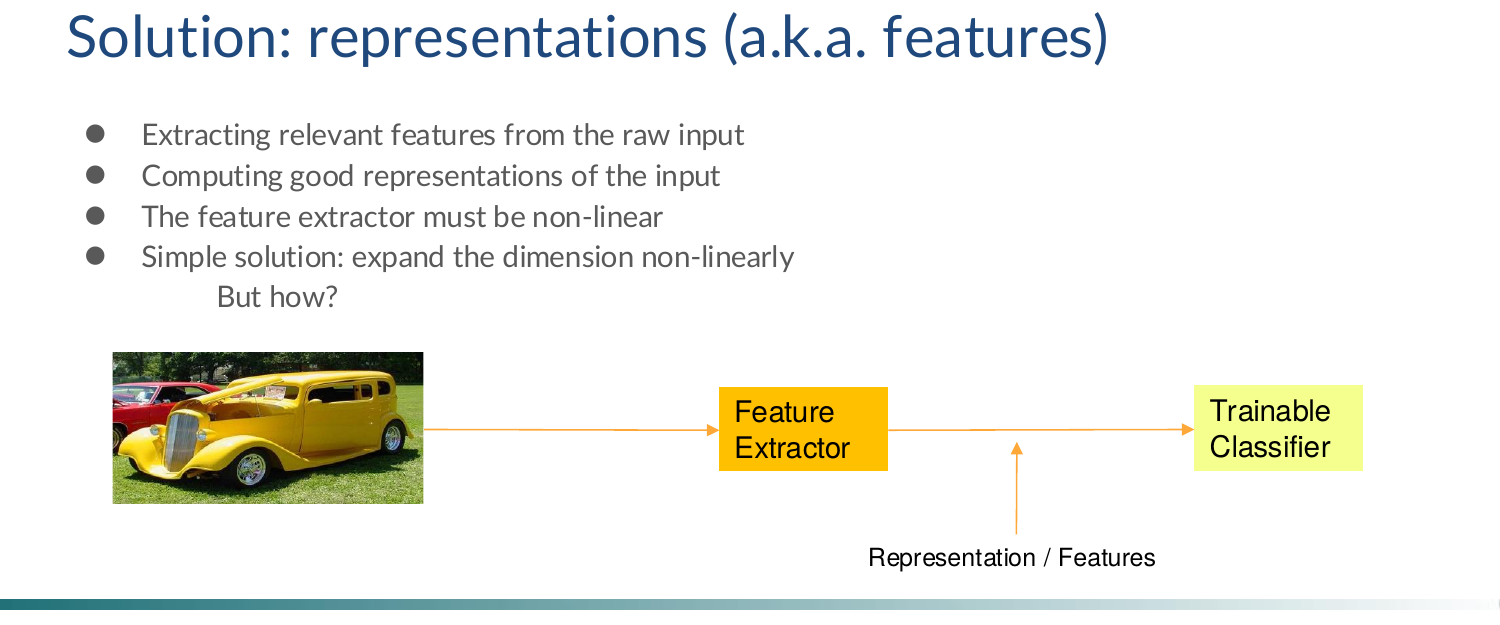
\includegraphics[width=0.80\linewidth]{figures/lr02_solution_repr.png}
  \caption{Soluzione con rappresentazioni: il blocco Feature Extractor
           trasforma l'input grezzo in una rappresentazione/feature; su queste
           opera un classificatore trainable. Nel DL anche l'estrattore è
           addestrato end-to-end.}
  \label{fig:solution_repr}
\end{figure}

Il principio di base è \textbf{espandere la dimensionalità} in modo non
lineare: in uno spazio di dimensione maggiore, punti che erano non separabili
diventano separabili con alta probabilità (per il Teorema di Cover, la
probabilità di separabilità cresce con $N$).

\subsection{Idee per l'estrazione generica di feature}

Esistono diverse strategie ``generiche'' per costruire feature non lineari
\reflecun{W2}:

\begin{itemize}
  \item \textbf{Space tiling}: si suddivide lo spazio di input in regioni e
        si usano indicatori di appartenenza come feature.
  \item \textbf{Random projections}: si proietta l'input su vettori casuali
        seguiti da non-linearità (es.\ ReLU). Alla base dei \textit{reservoir
        computing} e delle \textit{random features} per kernel approximation.
  \item \textbf{Feature monomiali} (cross-products): il feature extractor
        calcola prodotti di coppie (o triple, ecc.) di variabili di input;
        un classificatore lineare su queste feature calcola un polinomio
        dell'input.
  \item \textbf{Radial Basis Functions (RBF)}: feature del tipo
        $\phi_k(x) = \exp(-\|x - c_k\|^2 / 2\sigma^2)$, con centri $c_k$
        fissati o appresi.
  \item \textbf{Kernel machines}: generalizzano le RBF attraverso funzioni
        kernel $K(x^j, x)$; le SVM ne sono l'esempio principale.
\end{itemize}

\subsection{Feature monomiali e limiti}

\begin{figure}[H]
  \centering
  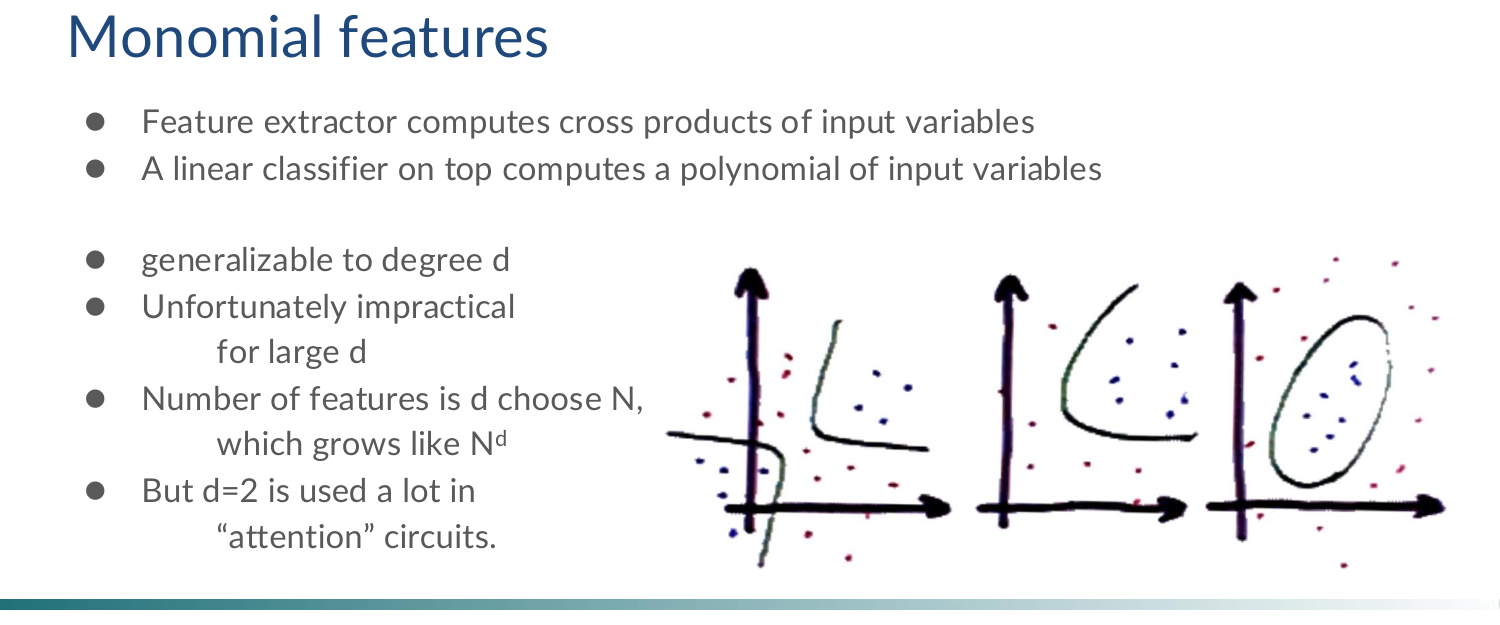
\includegraphics[width=0.82\linewidth]{figures/lr02_monomial.png}
  \caption{Feature monomiali: aggiungendo il termine quadratico $x_1 x_2$
           (o più in generale prodotti di grado $d$) come feature, un
           classificatore lineare può separare pattern che erano non lineari
           nell'input originale -- ad esempio boundary ellittici o a forma
           di C.}
  \label{fig:monomial}
\end{figure}

Le feature monomiali di grado $d$ su $N$ variabili producono
$\binom{N+d}{d} \sim N^d$ feature: questo numero cresce esponenzialmente con
$d$, rendendo il metodo impraticabile per grandi $d$.
Tuttavia, il caso $d=2$ è molto usato nei circuiti di
\textit{attention} (si veda il Cap.\,\ref{ch:basic-arch}), in quanto corrisponde
esattamente alle unità Sigma-Pi.

%------------------------------------------------------------
\section{Reti Shallow vs Reti Profonde}
\label{sec:shallow-vs-deep}

\subsection{Le reti shallow sono approssimatori universali}

Un risultato teorico fondamentale afferma che una rete neurale a 2 layer con
numero sufficiente di unità nascoste può approssimare qualsiasi funzione
continua con precisione arbitraria \refbishop{6}. Lo stesso vale per le
\textbf{Support Vector Machine} con kernel:
\begin{equation}
  G(X,\alpha) = \sum_j \alpha_j K(X^j, X),
\end{equation}
dove il primo layer calcola i kernel $K(X^j, X)$ usando i campioni di
training come template, e il secondo layer è una combinazione lineare con
pesi $\alpha_j$.

\begin{figure}[H]
  \centering
  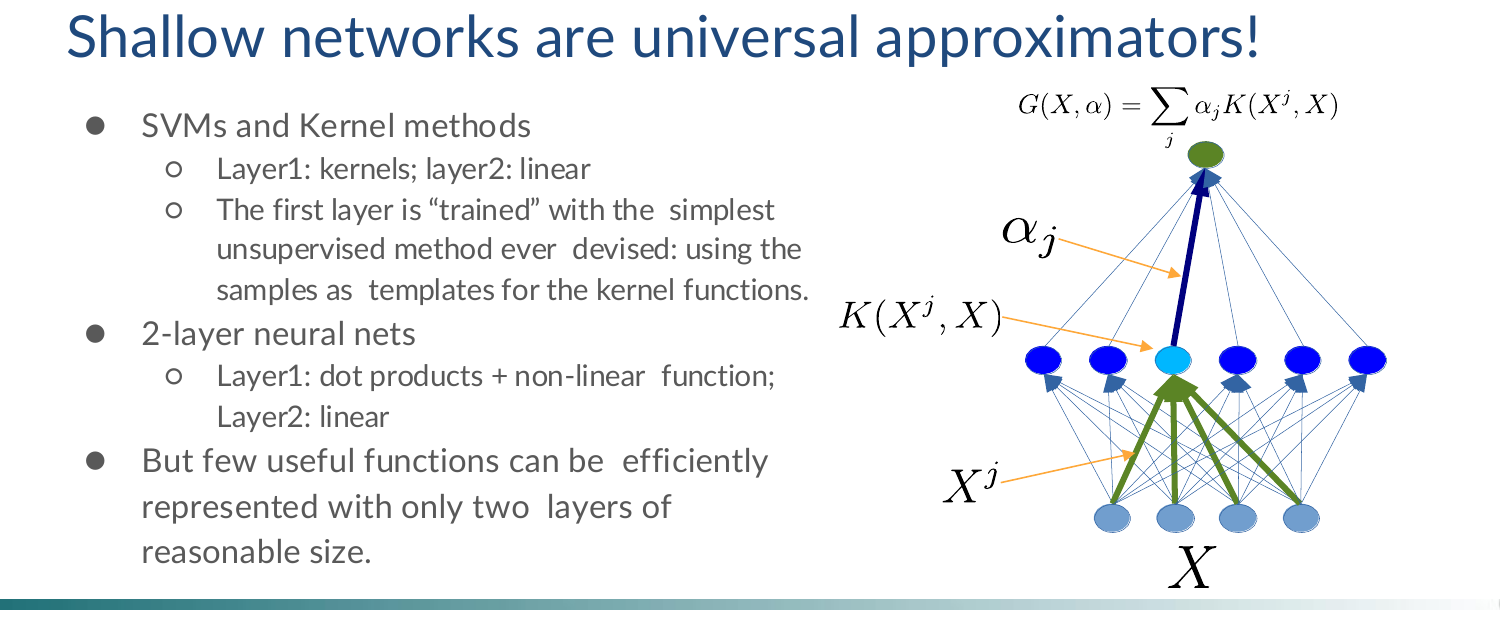
\includegraphics[width=0.80\linewidth]{figures/lr02_shallow_universal.png}
  \caption{Architettura di una kernel machine (SVM): il primo layer calcola
           $K(X^j, X)$ per ogni campione di training $X^j$; il secondo layer
           combina linearmente le attivazioni con pesi $\alpha_j$.}
  \label{fig:shallow_universal}
\end{figure}

\subsection{Perché servono architetture profonde?}

Se le reti shallow sono universali, perché usare reti profonde? Il
\textbf{dilemma del teorico} pone esattamente questa domanda.

\begin{figure}[H]
  \centering
  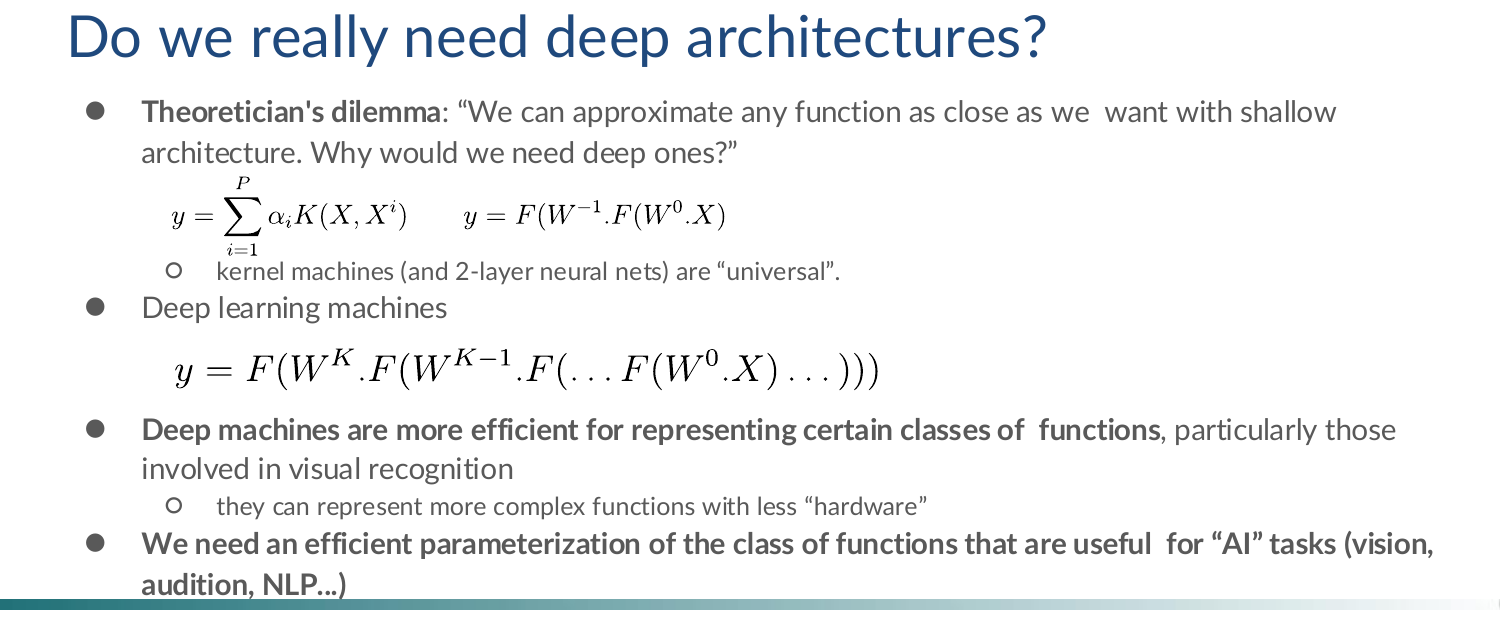
\includegraphics[width=0.88\linewidth]{figures/lr02_deep_vs_shallow.png}
  \caption{Confronto tra reti shallow e profonde: una rete shallow (kernel
           machine o 2-layer net) può rappresentare qualunque funzione, ma
           richiede un numero esponenziale di unità per funzioni complesse;
           una rete profonda $y = F(W^K \cdot F(\ldots F(W^0 \cdot X)\ldots))$
           le rappresenta in modo molto più efficiente.}
  \label{fig:deep_vs_shallow}
\end{figure}

La risposta è nell'\textbf{efficienza della rappresentazione}: le reti
profonde possono rappresentare certe classi di funzioni -- in particolare
quelle coinvolte nel riconoscimento visivo -- con molti meno parametri
rispetto alle reti shallow \citep{bishop2024}. Come argomenta
\citet{lecun2021}, una rete profonda \textit{scambia spazio con tempo}
(o ampiezza con profondità): più layer sequenziali ma meno hardware parallelo.

%------------------------------------------------------------
\section{Invariant Feature Learning}
\label{sec:invariant-features}

L'idea di base per imparare feature invarianti è la seguente
\reflecun{W2}:

\begin{enumerate}
  \item \textbf{Espandere} l'input non linearmente in uno spazio ad alta
        dimensionalità (feature instabili ma discriminative).
  \item \textbf{Aggregare} regioni del nuovo spazio (pooling, proiezione,
        riduzione di dimensionalità) per ottenere feature stabili e invarianti.
\end{enumerate}

\begin{figure}[H]
  \centering
  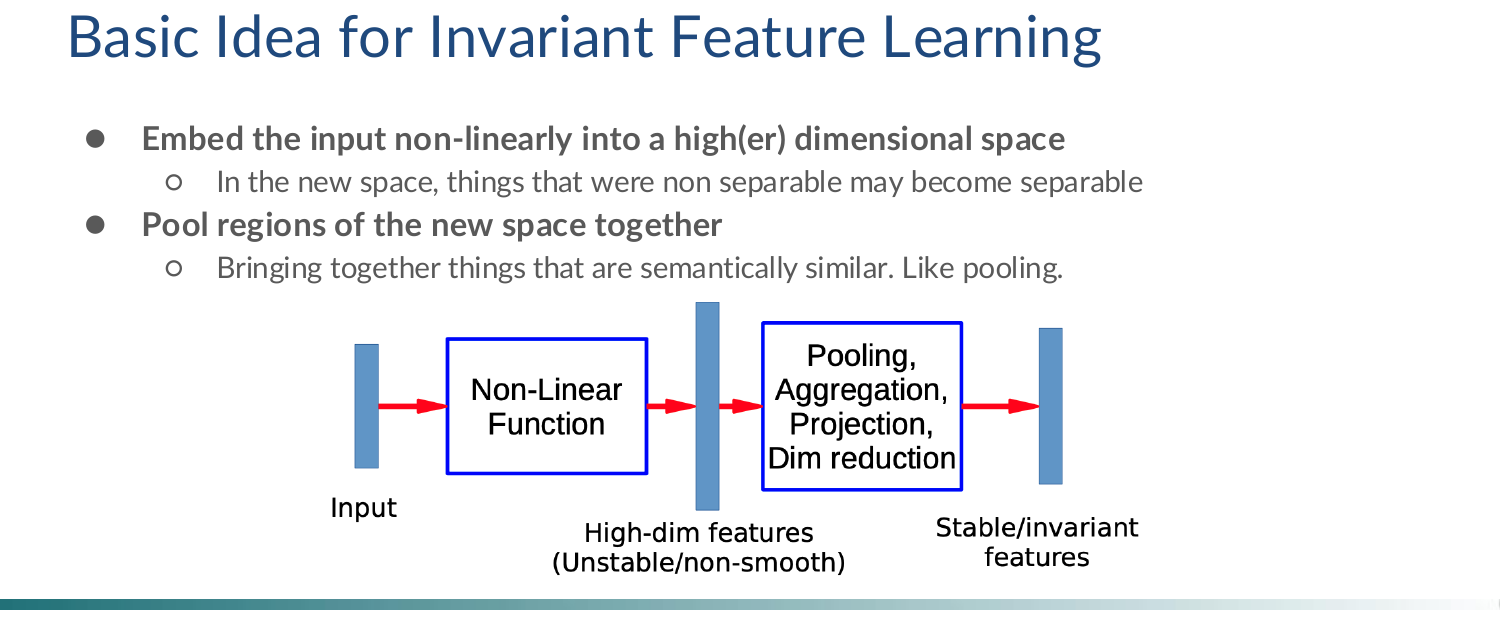
\includegraphics[width=0.82\linewidth]{figures/lr02_invariant_learning.png}
  \caption{Schema dell'invariant feature learning: la funzione non lineare
           espande l'input in feature ad alta dimensione (instabili), che
           vengono poi aggregate tramite pooling/aggregazione/dim.\
           reduction per produrre feature stabili e invarianti.}
  \label{fig:invariant_learning}
\end{figure}

%------------------------------------------------------------
\section{L'Ipotesi del Manifold}
\label{sec:manifold}

\begin{definizione}[Manifold Hypothesis]
I dati naturali vivono in un \textbf{manifold non lineare a bassa dimensione}
immerso nello spazio ad alta dimensione. Le variabili nei dati naturali sono
mutuamente dipendenti, per cui la variabilità intrinseca è molto più bassa
della dimensione nominale.
\end{definizione}

\begin{figure}[H]
  \centering
  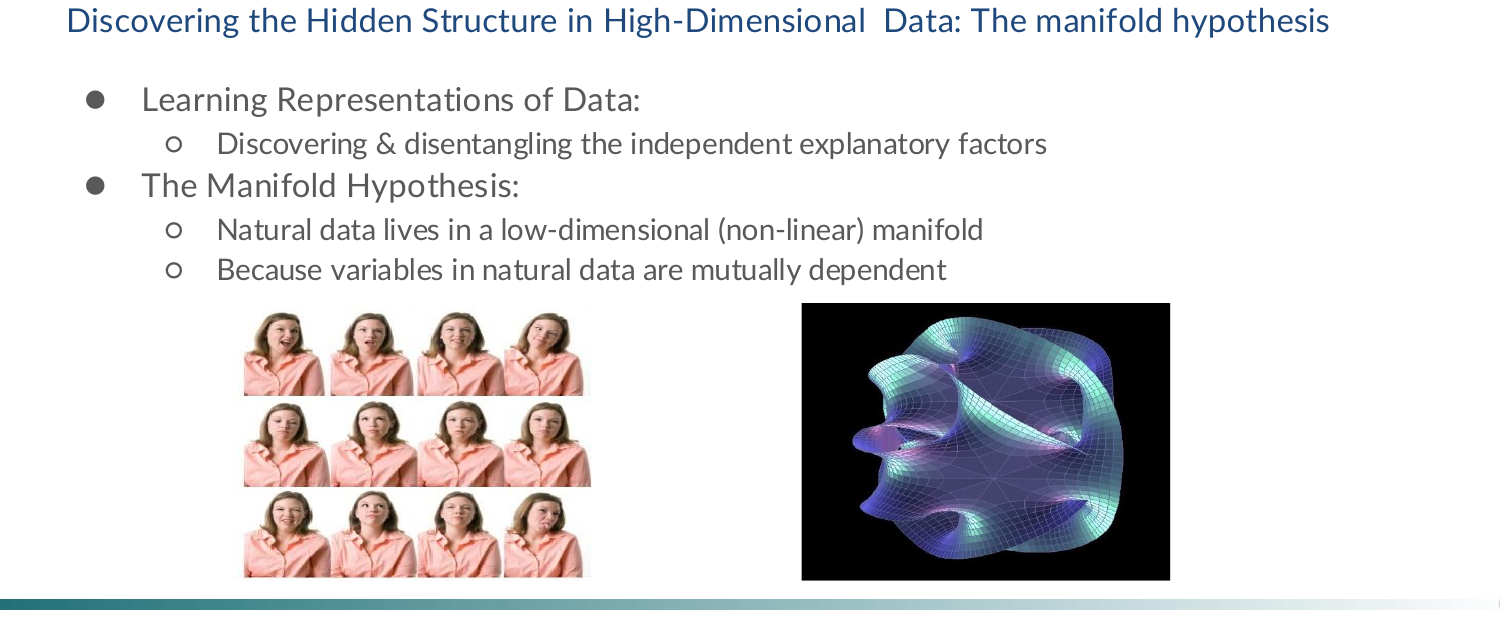
\includegraphics[width=0.88\linewidth]{figures/lr02_manifold_hypothesis.png}
  \caption{L'ipotesi del manifold: le immagini di volti (sinistra) variano
           in espressione, posa, illuminazione -- ma questa variabilità
           appartiene a un manifold a bassa dimensione (destra), non a tutto
           lo spazio dei pixel.}
  \label{fig:manifold_hypothesis}
\end{figure}

\paragraph{Esempio: immagini di volti.}
Un'immagine $1000 \times 1000$ pixel ha $10^6$ dimensioni. Tuttavia un volto
è descritto da soli 3 coordinate cartesiane, 3 angoli di Eulero e meno di 50
muscoli facciali: il manifold delle immagini di un volto ha quindi meno di 56
dimensioni effettive.

\begin{figure}[H]
  \centering
  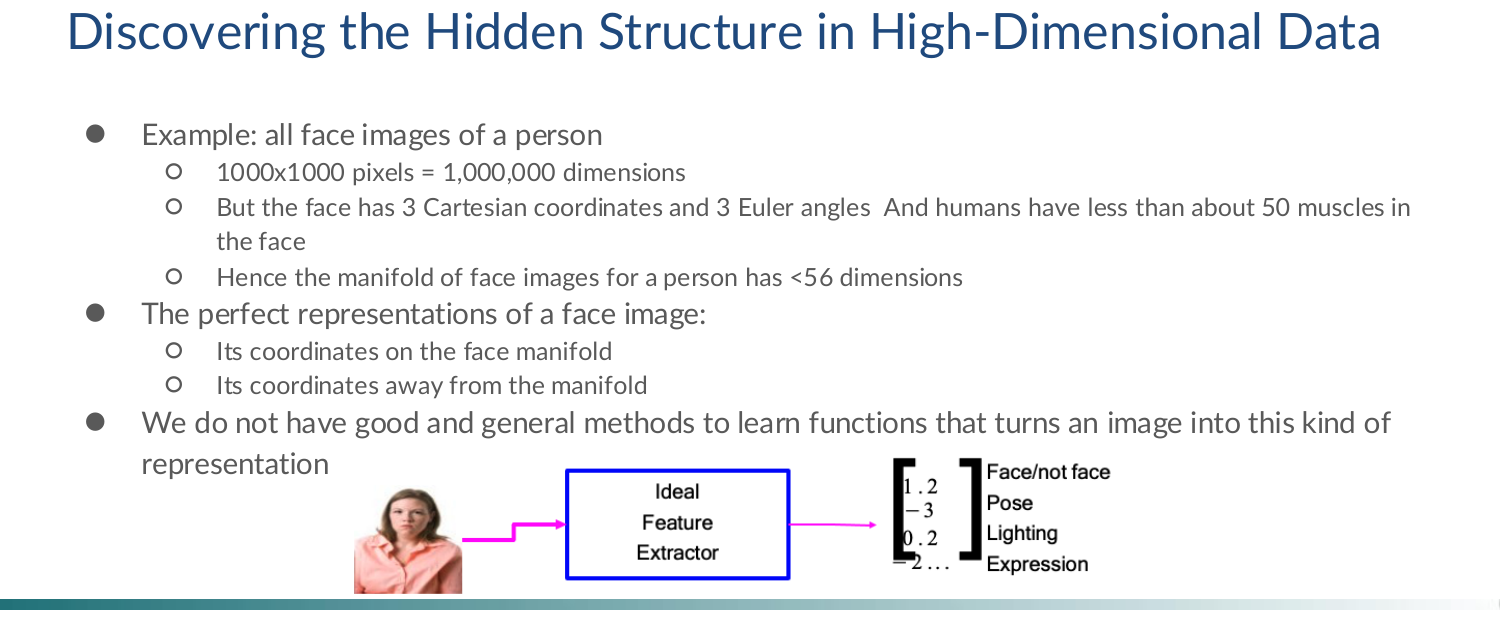
\includegraphics[width=0.82\linewidth]{figures/lr02_face_manifold.png}
  \caption{La rappresentazione ideale di un'immagine facciale ne estrae le
           coordinate sul manifold (pose, lighting, expression\ldots) come
           vettore compatto. Non disponiamo ancora di metodi generali per
           imparare questa funzione.}
  \label{fig:face_manifold}
\end{figure}

%------------------------------------------------------------
\section{Disentangling e Apprendimento delle Rappresentazioni}
\label{sec:disentangling}

L'obiettivo del \textbf{representation learning} è scoprire e
\emph{disintrecciare} (disentangle) i fattori di variazione indipendenti
che generano i dati.

\begin{figure}[H]
  \centering
  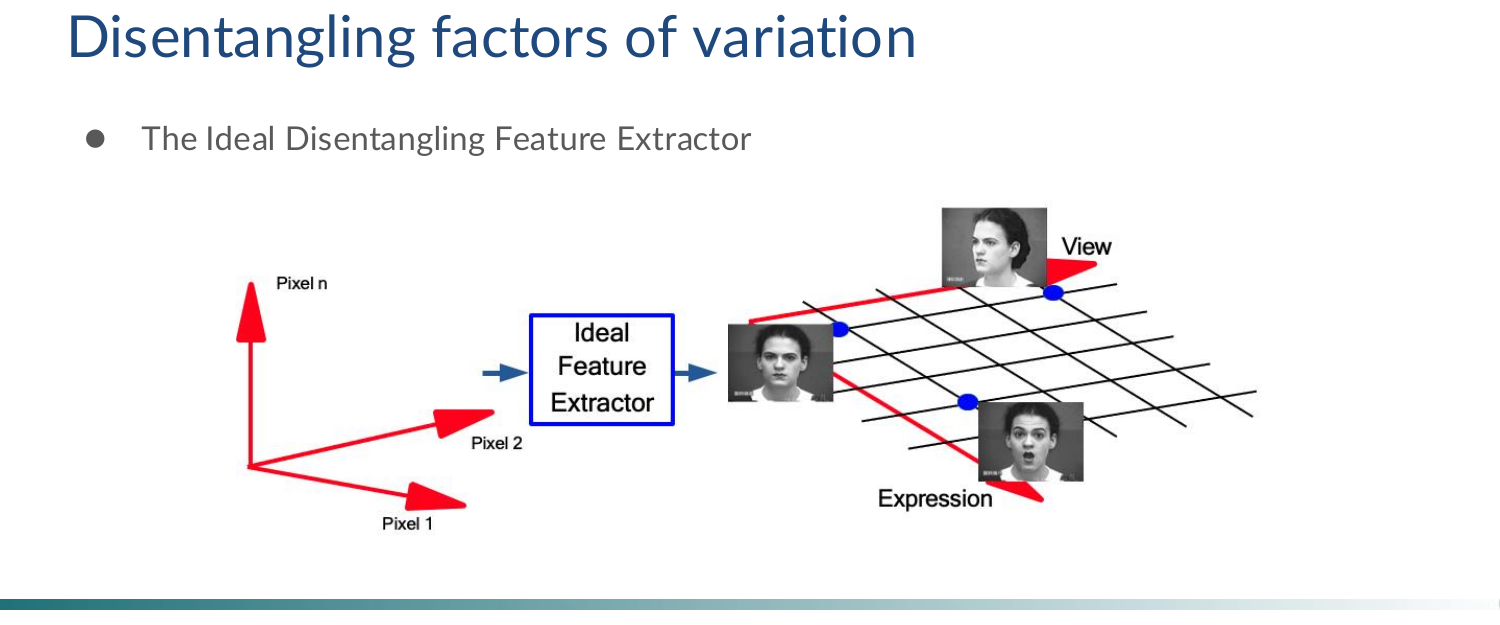
\includegraphics[width=0.88\linewidth]{figures/lr02_disentangling.png}
  \caption{L'ideal feature extractor mappa lo spazio dei pixel (sinistra)
           nel manifold dei volti (destra), dove le coordinate corrispondono
           a fattori interpretabili come ``view'' (punto di vista) e
           ``expression'' (espressione). Ogni punto blu nel manifold
           corrisponde a un'immagine specifica.}
  \label{fig:disentangling}
\end{figure}

Un esempio concreto di manifold appreso è mostrato nel lavoro di
Hadsell et al.\ (CVPR 2006): immagini di aeroplani in diverse rotazioni
sono disposte su una curva chiusa nell'embedding space, rispecchiando
la struttura continua della rotazione.

\begin{figure}[H]
  \centering
  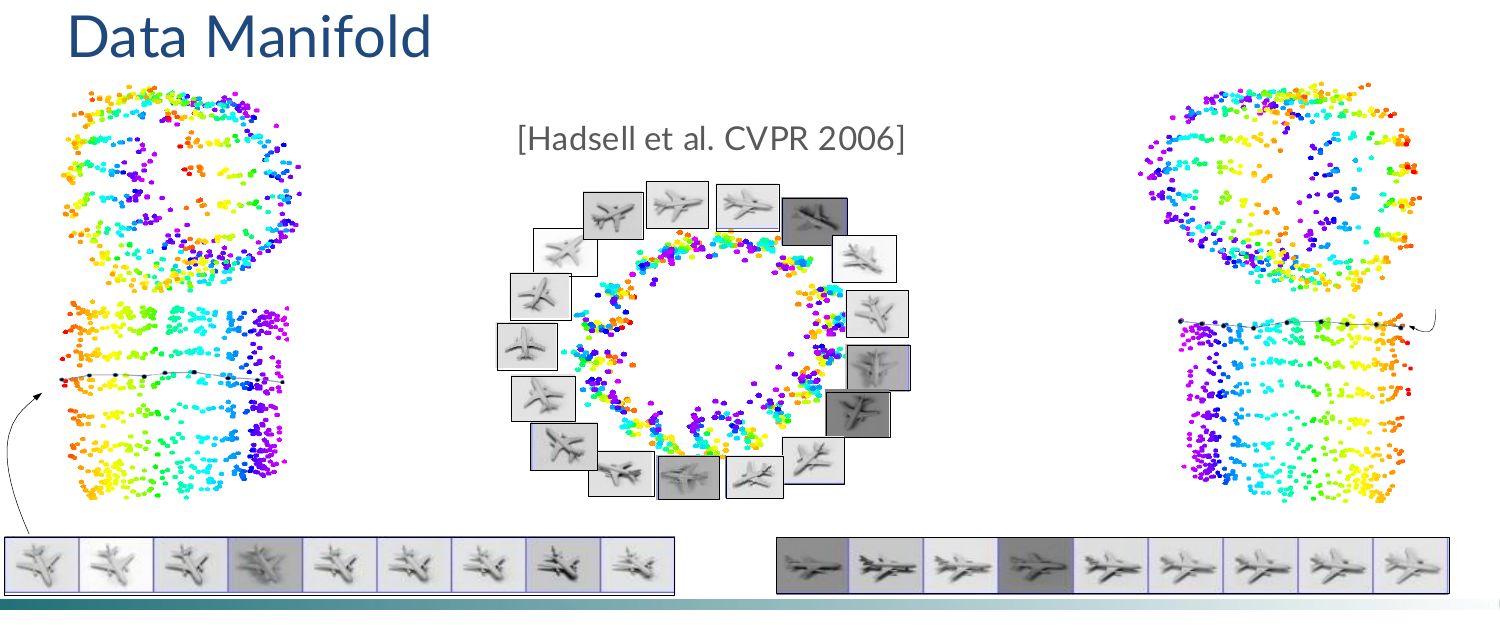
\includegraphics[width=0.88\linewidth]{figures/lr02_data_manifold.png}
  \caption{Data manifold appreso [Hadsell et al., CVPR 2006]: le immagini
           di aeroplani in diverse orientazioni formano una struttura ciclica
           coerente nello spazio di embedding -- punti vicini corrispondono a
           immagini visivamente simili.}
  \label{fig:data_manifold}
\end{figure}

%------------------------------------------------------------
\section{Architetture Multilayer = Struttura Compositiva}
\label{sec:multilayer}

I dati naturali hanno una \textbf{struttura compositiva}: sono costruiti
gerarchicamente da elementi via via più astratti. Le reti neurali multilayer
sfruttano questa struttura, con ogni layer che apprende un livello di
astrazione \citep{lecun2021}.

\begin{figure}[H]
  \centering
  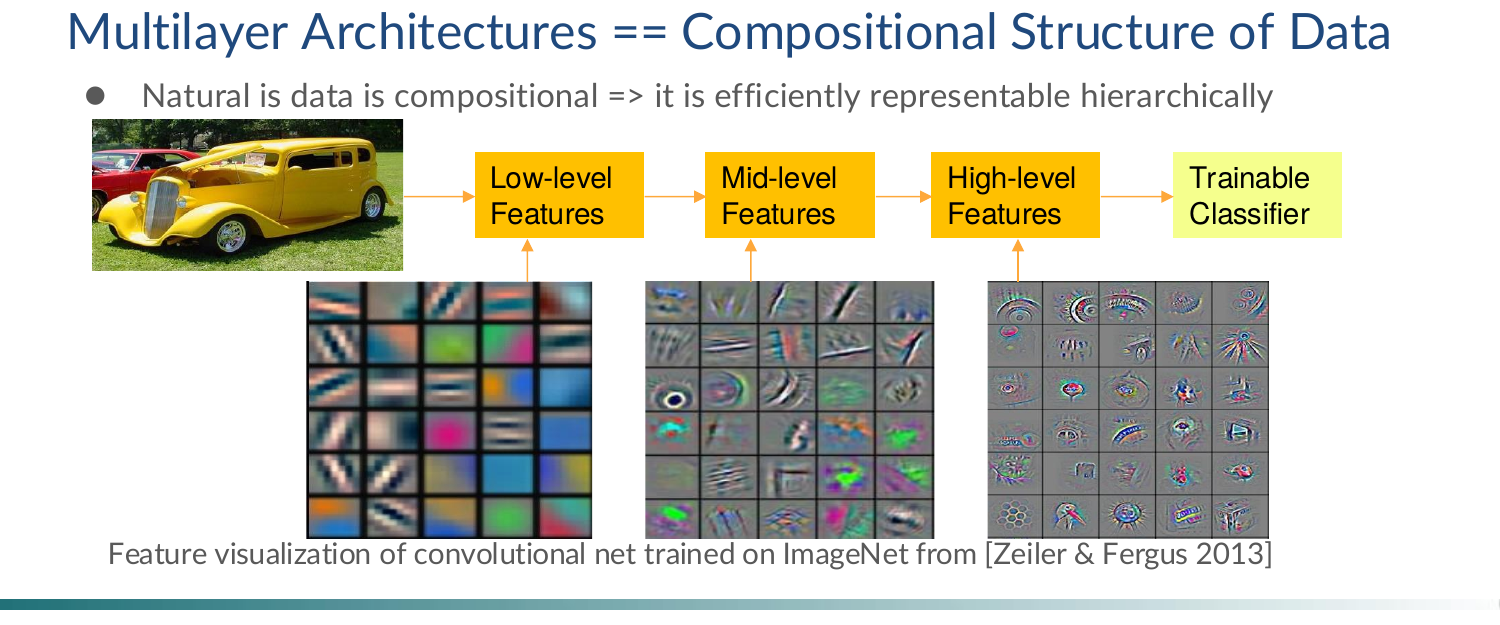
\includegraphics[width=0.92\linewidth]{figures/lr02_compositional.png}
  \caption{Le architetture multilayer corrispondono alla struttura compositiva
           dei dati. La visualizzazione delle feature di una CNN addestrata su
           ImageNet [Zeiler \& Fergus, 2013] mostra: layer bassi = edge e
           texture, layer intermedi = parti di oggetti, layer alti = concetti
           semantici.}
  \label{fig:compositional}
\end{figure}

\paragraph{Gerarchia di rappresentazioni nei diversi domini.}

\begin{figure}[H]
  \centering
  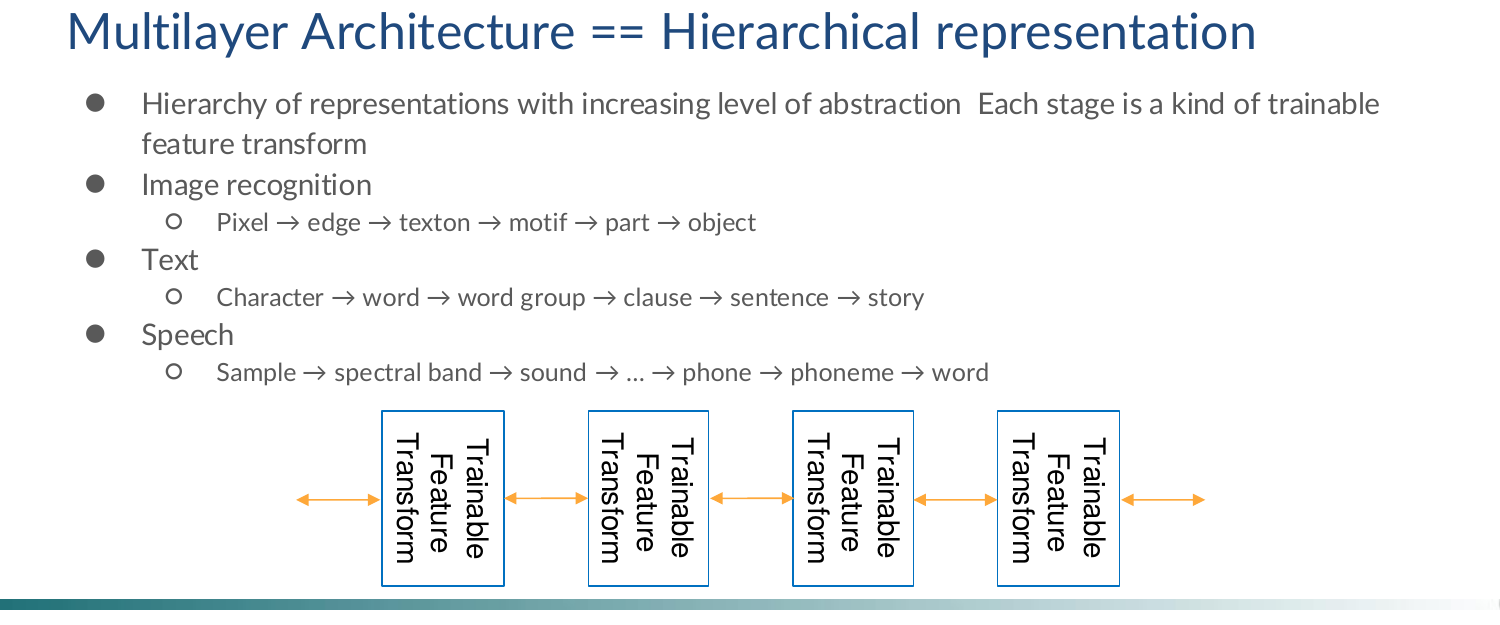
\includegraphics[width=0.82\linewidth]{figures/lr02_hierarchical.png}
  \caption{Architettura multilayer come rappresentazione gerarchica: ogni
           blocco ``Trainable Feature Transform'' corrisponde a un livello di
           astrazione. Le frecce bidirezionali indicano che ogni modulo
           può essere addestrato con backpropagation.}
  \label{fig:hierarchical}
\end{figure}

La gerarchia di astrazioni varia a seconda del dominio:
\begin{itemize}
  \item \textbf{Immagini}: pixel $\to$ edge $\to$ texton $\to$ motif
        $\to$ parte $\to$ oggetto.
  \item \textbf{Testo}: carattere $\to$ parola $\to$ gruppo di parole
        $\to$ proposizione $\to$ frase $\to$ storia.
  \item \textbf{Audio}: campione $\to$ banda spettrale $\to$ suono
        $\to$ \ldots $\to$ fonema $\to$ parola.
\end{itemize}

L'efficienza delle architetture profonde è spiegata da
\citet{lecun2021} e da Bengio \& LeCun (2007): una rete profonda
\textit{scambia ampiezza con profondità} -- più layer sequenziali ma
meno hardware parallelo -- riuscendo a rappresentare funzioni complesse
con molti meno parametri rispetto a una rete shallow.

%------------------------------------------------------------
\section{Riepilogo}
\label{sec:summary-ch2}

\begin{center}
\begin{tabular}{lll}
  \toprule
  \textbf{Concetto} & \textbf{Idea chiave} & \textbf{Implicazione} \\
  \midrule
  Classificatore lineare & $\bar{y}=\operatorname{sign}(\vect{w}^T\vect{x}+b)$ & Limite: non sep. lineare \\
  Teorema di Cover       & Prob.\ sep.\ $\to 0$ se $P \gg N$      & Serve non-linearità \\
  Feature monomiali      & Cross-products di grado $d$             & $O(N^d)$ feature \\
  Reti shallow           & Approssimatori universali               & Ma inefficienti \\
  Reti profonde          & $y = F(W^K \cdot F(\ldots))$           & Più efficienti \\
  Manifold Hypothesis    & Dati su manifold bassa-dim.             & Motiva il DL \\
  Disentangling          & Separare i fattori di variazione        & Obiettivo del repr.\ learning \\
  Struttura compositiva  & Pixel $\to$ edge $\to$ parte $\to$ obj & Giustifica i multilayer \\
  \bottomrule
\end{tabular}
\end{center}

Le reti neurali profonde sono giustificate non solo dall'approssimazione
universale (che vale anche per reti shallow), ma dalla loro
\textbf{efficienza parametrica} nel rappresentare le funzioni utili per i
compiti AI. L'ipotesi del manifold e la struttura compositiva dei dati
naturali forniscono le basi teoriche per questa efficienza.

% %============================================================
%  Capitolo 3 – Activation Functions
%============================================================
\chapter{Activation Functions}
\label{ch:activation-functions}

Le \textbf{funzioni di attivazione} sono il cuore della non-linearità nelle reti neurali.
Senza di esse, una rete a più strati si ridurrebbe a una semplice trasformazione lineare,
indipendentemente dalla profondità \citep{bishop2024}.
Come osserva Canziani nelle note NYU-DL, ogni layer di una rete tradizionale alterna
un blocco \emph{lineare} $\mathbf{s}_{k+1} = W_k \mathbf{z}_k$ a un blocco \emph{non lineare}
$\mathbf{z}_k = h(\mathbf{s}_k)$, dove $h$ è appunto la funzione di attivazione.
La scelta di $h$ influenza profondamente la velocità di convergenza, la stabilità
del gradiente e le capacità espressive della rete.

%------------------------------------------------------------
\section{Il Problema del Vanishing Gradient}
\label{sec:vanishing-gradient}

Il principale limite delle funzioni di attivazione \textbf{saturanti} (es.\ Sigmoid,
Tanh) è il cosiddetto \textbf{vanishing gradient problem}.
La retropropagazione moltiplica gradienti attraverso ogni layer: se ogni fattore è
$\ll 1$, il segnale si azzera esponenzialmente procedendo verso i layer iniziali.

Per la Sigmoid, il gradiente massimo è:
\begin{equation}
  \max_x \frac{\partial\,\sigma(x)}{\partial x}
  = \frac{1}{4} = 0{,}25 \qquad \text{(raggiunto in } x=0\text{)},
\end{equation}
e si avvicina a zero sia per $x \to +\infty$ sia per $x \to -\infty$.
In una rete con $L$ layer, il gradiente che torna al primo layer scala come
$(0{,}25)^L$: già per $L=10$ si ottiene $\approx 10^{-6}$.

\begin{figure}[H]
  \centering
  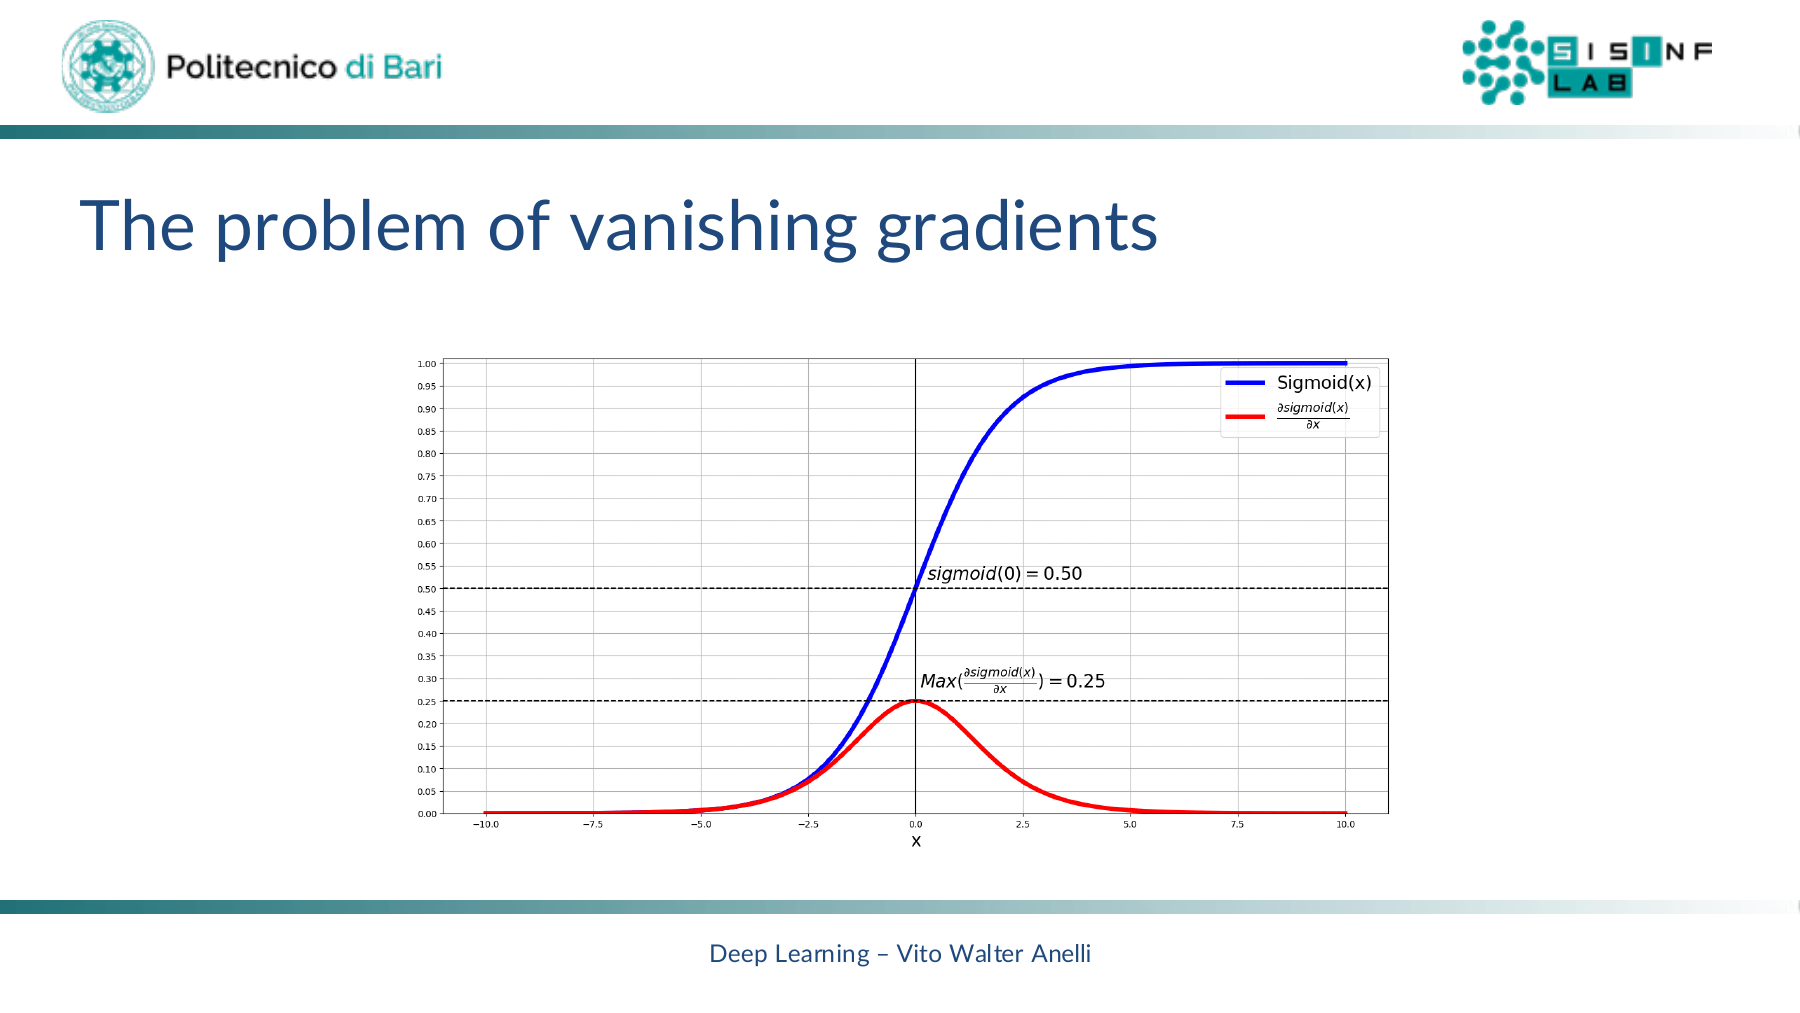
\includegraphics[width=0.82\linewidth]{figures/af03_vanishing_gradient.png}
  \caption{Sigmoid e sua derivata. Il valore $\sigma(0)=0{,}5$ è il punto di inflessione
           e il gradiente massimo è $0{,}25$. Per input molto grandi o molto piccoli
           la derivata tende a zero, bloccando il flusso del gradiente nei layer
           profondi.}
  \label{fig:vanishing_gradient}
\end{figure}

La soluzione più efficace è passare a funzioni \textbf{non saturanti} per i layer
interni, riservando funzioni saturanti solo all'output quando la struttura del
problema lo richiede (es.\ classificazione binaria, gating nelle LSTM).

%------------------------------------------------------------
\section{Panoramica: Saturating vs Non-Saturating}
\label{sec:overview-activations}

\begin{figure}[H]
  \centering
  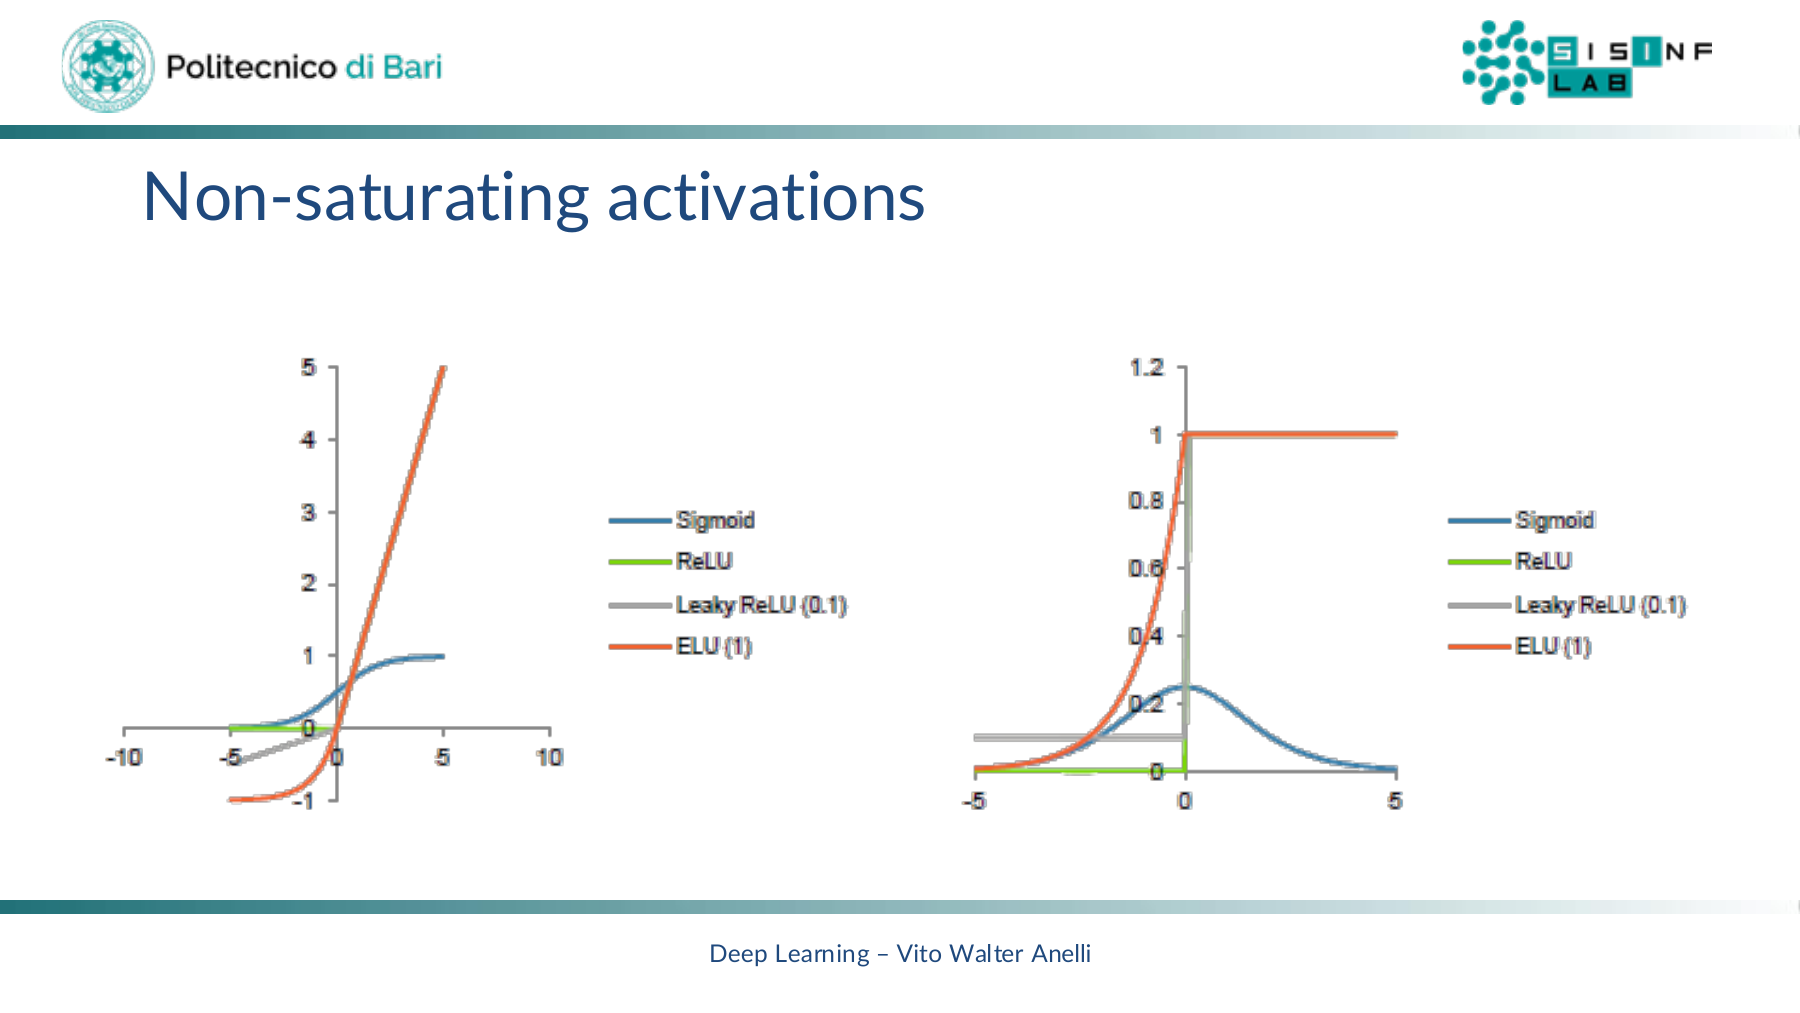
\includegraphics[width=0.90\linewidth]{figures/af03_nonsaturating_overview.png}
  \caption{Confronto visivo tra funzioni di attivazione saturanti e non saturanti
           (Sigmoid, ReLU, Leaky ReLU, ELU) nelle loro curve e nelle rispettive derivate.
           Le funzioni non saturanti mantengono un gradiente costante nella regione
           positiva, risolvendo il vanishing gradient.}
  \label{fig:nonsaturating_overview}
\end{figure}

%------------------------------------------------------------
\section{Famiglia ReLU}
\label{sec:relu-family}

\subsection{ReLU -- \texttt{nn.ReLU()}}
\label{subsec:relu}

La \textbf{Rectified Linear Unit} (ReLU) è oggi la funzione di attivazione di
default per i layer nascosti delle reti profonde \citep{bishop2024}:

\begin{equation}
  \operatorname{ReLU}(x) = (x)^{+} = \max(0, x).
\end{equation}

\begin{figure}[H]
  \centering
  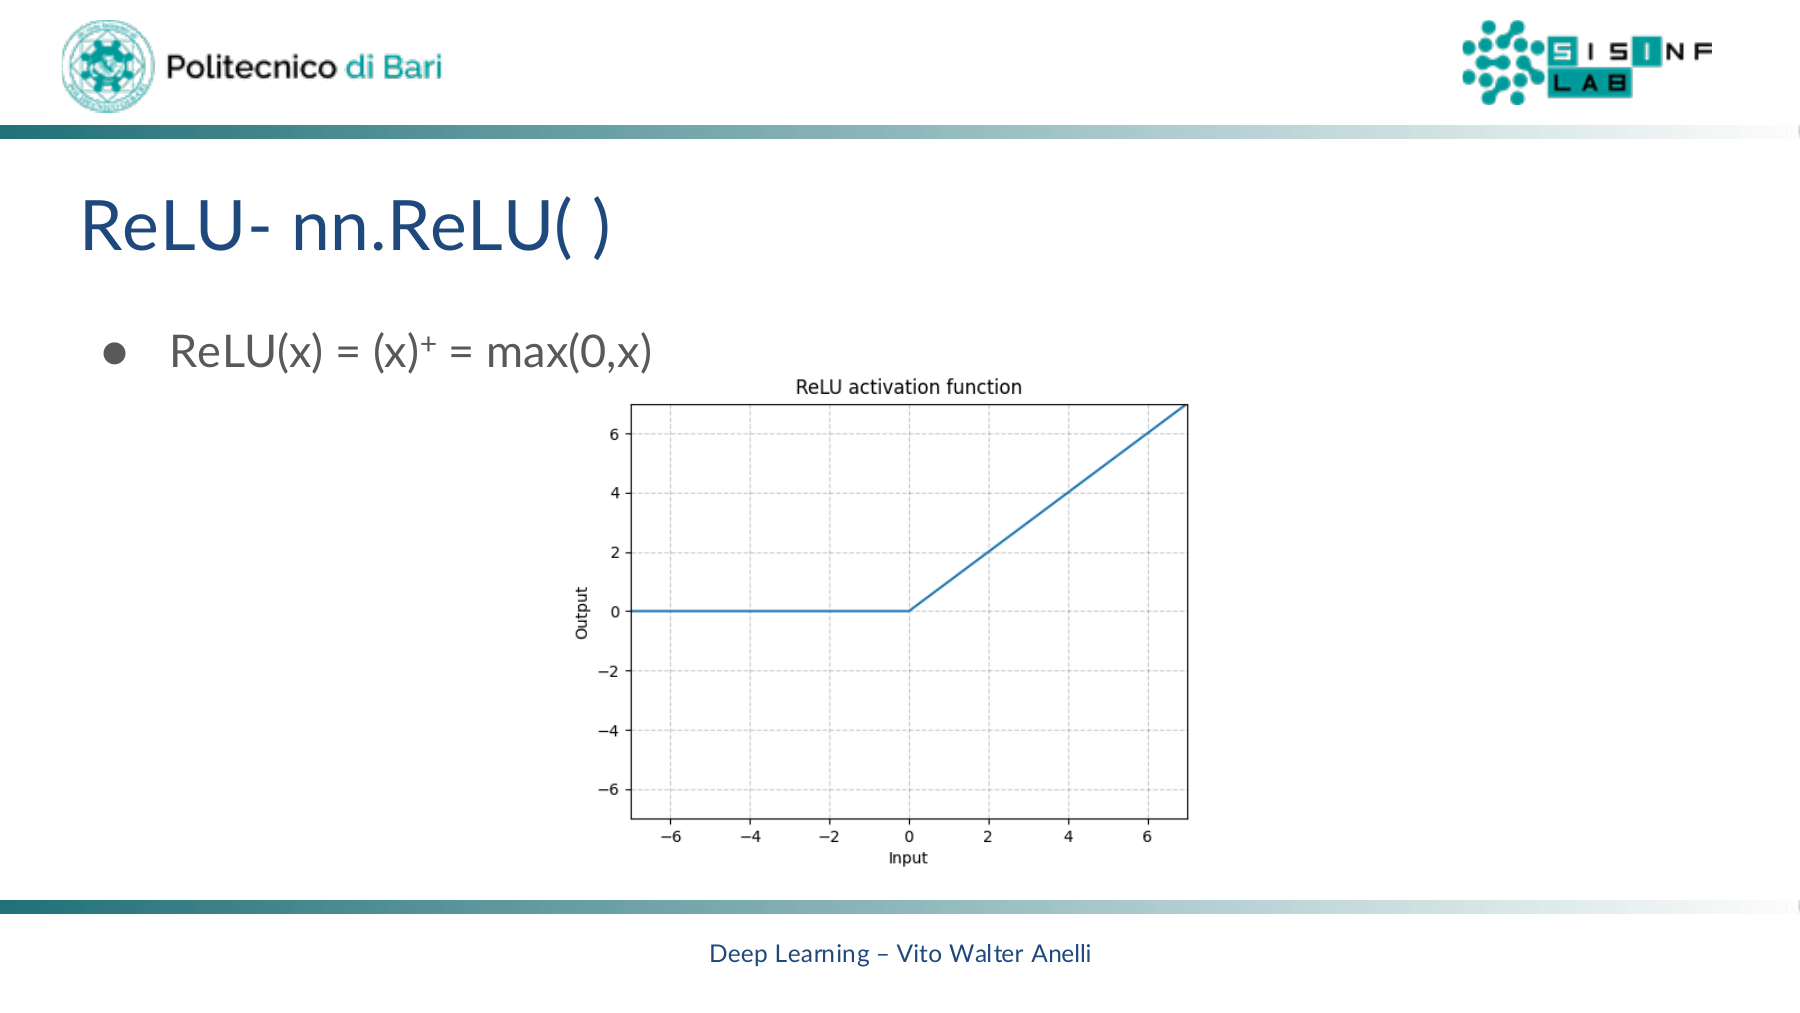
\includegraphics[width=0.72\linewidth]{figures/af03_relu.png}
  \caption{ReLU: uscita identità per $x \geq 0$, zero per $x < 0$.
           La derivata è discontinua in $x=0$ ma il gradiente è $1$ per tutti
           gli input positivi, eliminando completamente il vanishing gradient
           nel ramo attivo.}
  \label{fig:relu}
\end{figure}

\paragraph{Proprietà chiave.}
\begin{itemize}
  \item \textbf{Efficienza computazionale}: riduce a un semplice confronto con zero.
  \item \textbf{Gradiente non saturante}: la derivata è $1$ per $x>0$, evitando
        il vanishing gradient.
  \item \textbf{Sparsità}: i neuroni con input negativo producono esattamente zero,
        inducendo rappresentazioni sparse che migliorano la generalizzazione.
  \item \textbf{Dead ReLU problem}: se un neurone riceve input sempre negativi
        (es.\ dopo un grande aggiornamento del gradiente), il suo gradiente sarà
        sempre zero e il neurone cessa di apprendere. Le varianti seguenti
        mitigano questo problema.
\end{itemize}

\subsection{Leaky ReLU -- \texttt{nn.LeakyReLU()}}
\label{subsec:leaky-relu}

\begin{equation}
  \operatorname{LeakyReLU}(x) =
  \begin{cases}
    x,                                  & \text{se } x \geq 0 \\
    a_{\text{negative\_slope}} \times x, & \text{altrimenti}
  \end{cases}
\end{equation}

dove $a_{\text{negative\_slope}}$ è una piccola costante (tipicamente $0{,}01$).

\begin{figure}[H]
  \centering
  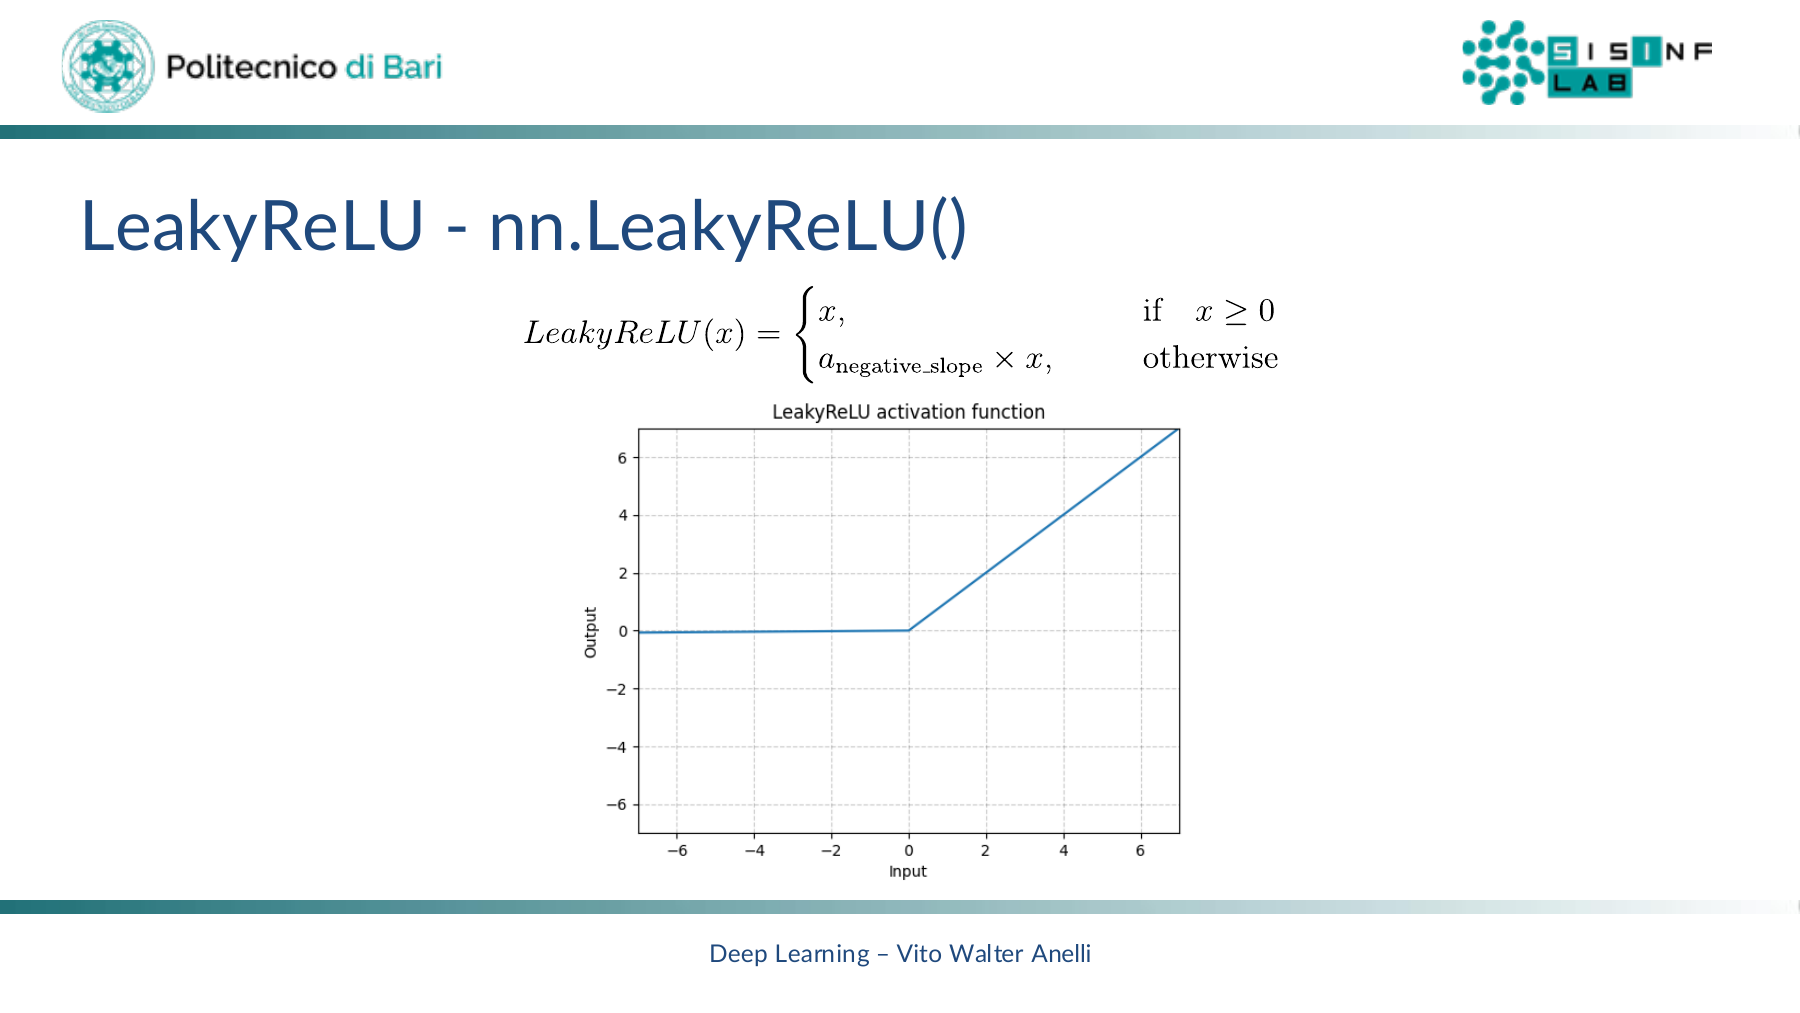
\includegraphics[width=0.72\linewidth]{figures/af03_leaky_relu.png}
  \caption{Leaky ReLU: introduce una piccola pendenza nella regione negativa
           ($a_{\text{neg}}=0{,}1$ nella figura), consentendo al gradiente di
           fluire anche per neuroni con input negativo e risolvendo il
           \emph{dead neuron} problem.}
  \label{fig:leaky_relu}
\end{figure}

Rispetto a ReLU, Leaky ReLU garantisce un gradiente non nullo anche per $x<0$,
mantenendo i neuroni attivi durante l'intero training.
Il coefficiente $a$ è fisso e scelto prima del training.

\subsection{PReLU -- \texttt{nn.PReLU()}}
\label{subsec:prelu}

\begin{equation}
  \operatorname{PReLU}(x) =
  \begin{cases}
    x,  & \text{se } x \geq 0 \\
    ax, & \text{altrimenti}
  \end{cases}
\end{equation}

\begin{figure}[H]
  \centering
  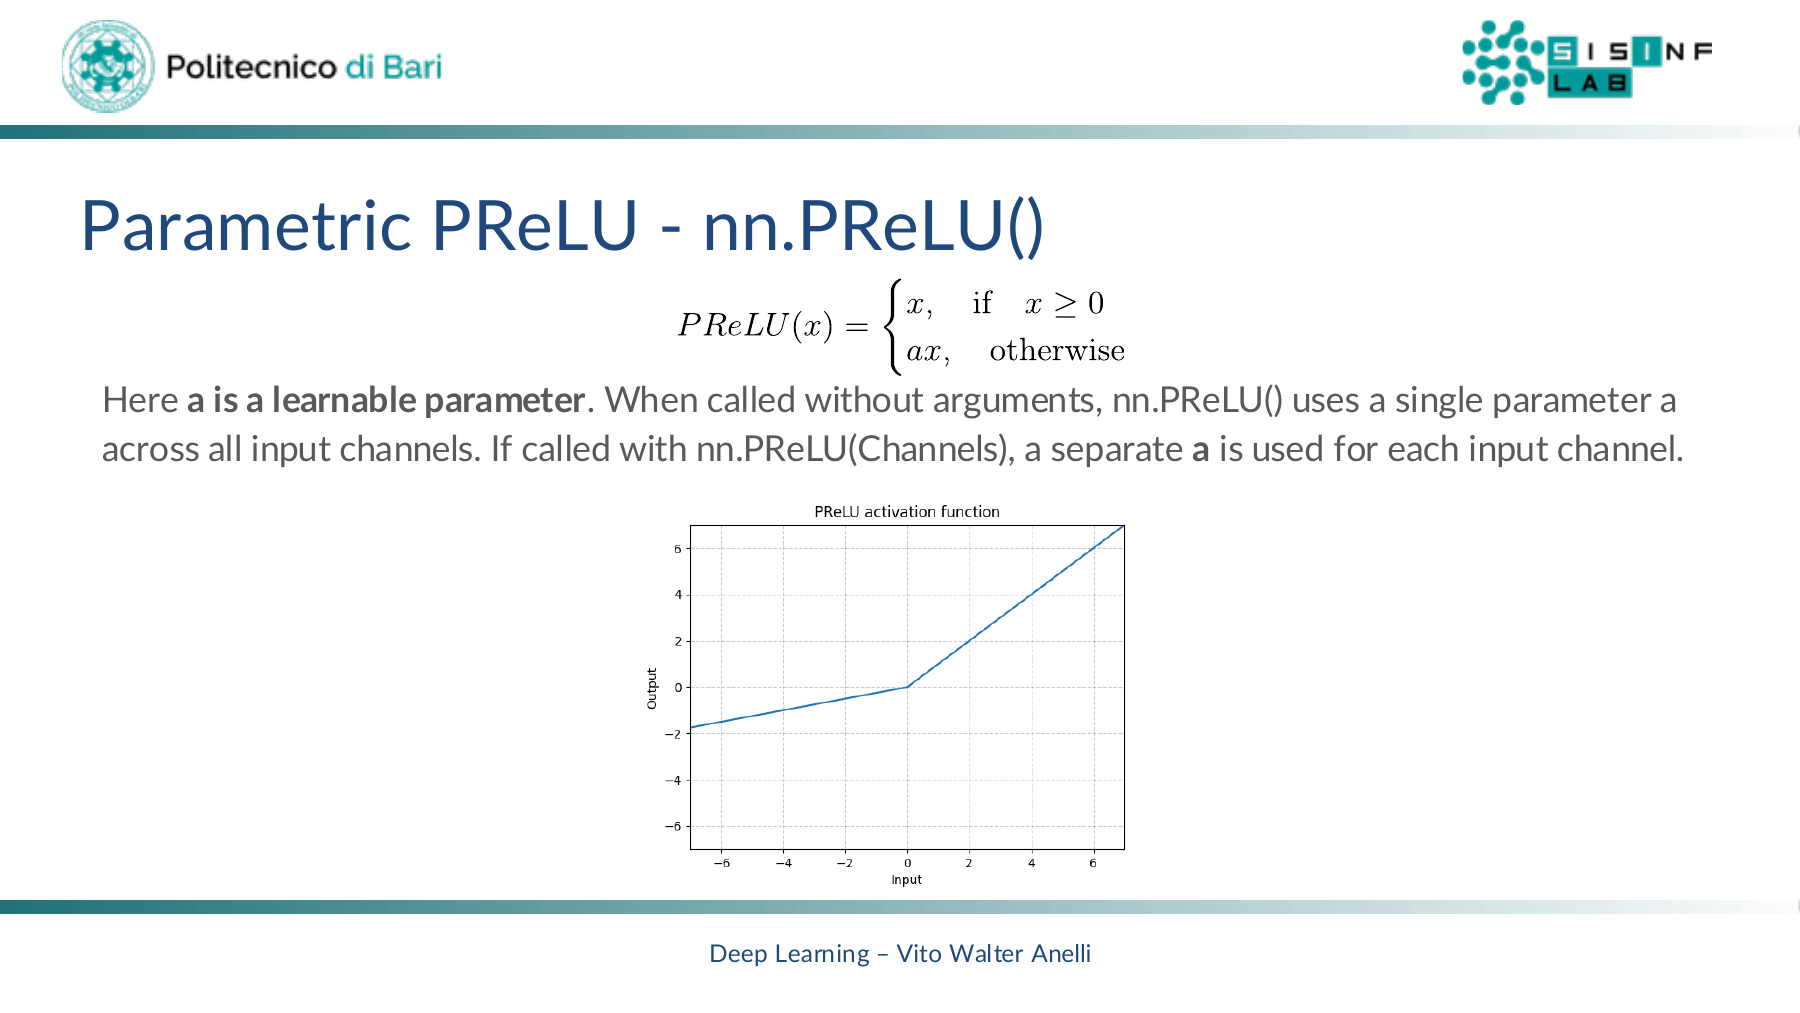
\includegraphics[width=0.72\linewidth]{figures/af03_prelu.png}
  \caption{Parametric ReLU (PReLU): il coefficiente $a$ è un \textbf{parametro
           apprendibile} con la retropropagazione. Chiamato senza argomenti,
           \texttt{nn.PReLU()} usa un unico parametro $a$ condiviso; chiamato
           con \texttt{nn.PReLU(C)}, usa un $a$ distinto per ognuno degli $C$
           canali in input.}
  \label{fig:prelu}
\end{figure}

La distinzione tra le tre varianti è riassumibile come segue:
\textbf{LReLU} usa un $a$ fisso, \textbf{PReLU} apprende $a$,
\textbf{RReLU} campiona $a$ casualmente durante il training.

\subsection{RReLU -- \texttt{nn.RReLU()}}
\label{subsec:rrelu}

\begin{equation}
  \operatorname{RReLU}(x) =
  \begin{cases}
    x,  & \text{se } x \geq 0 \\
    ax, & \text{altrimenti}
  \end{cases}
\end{equation}

\begin{figure}[H]
  \centering
  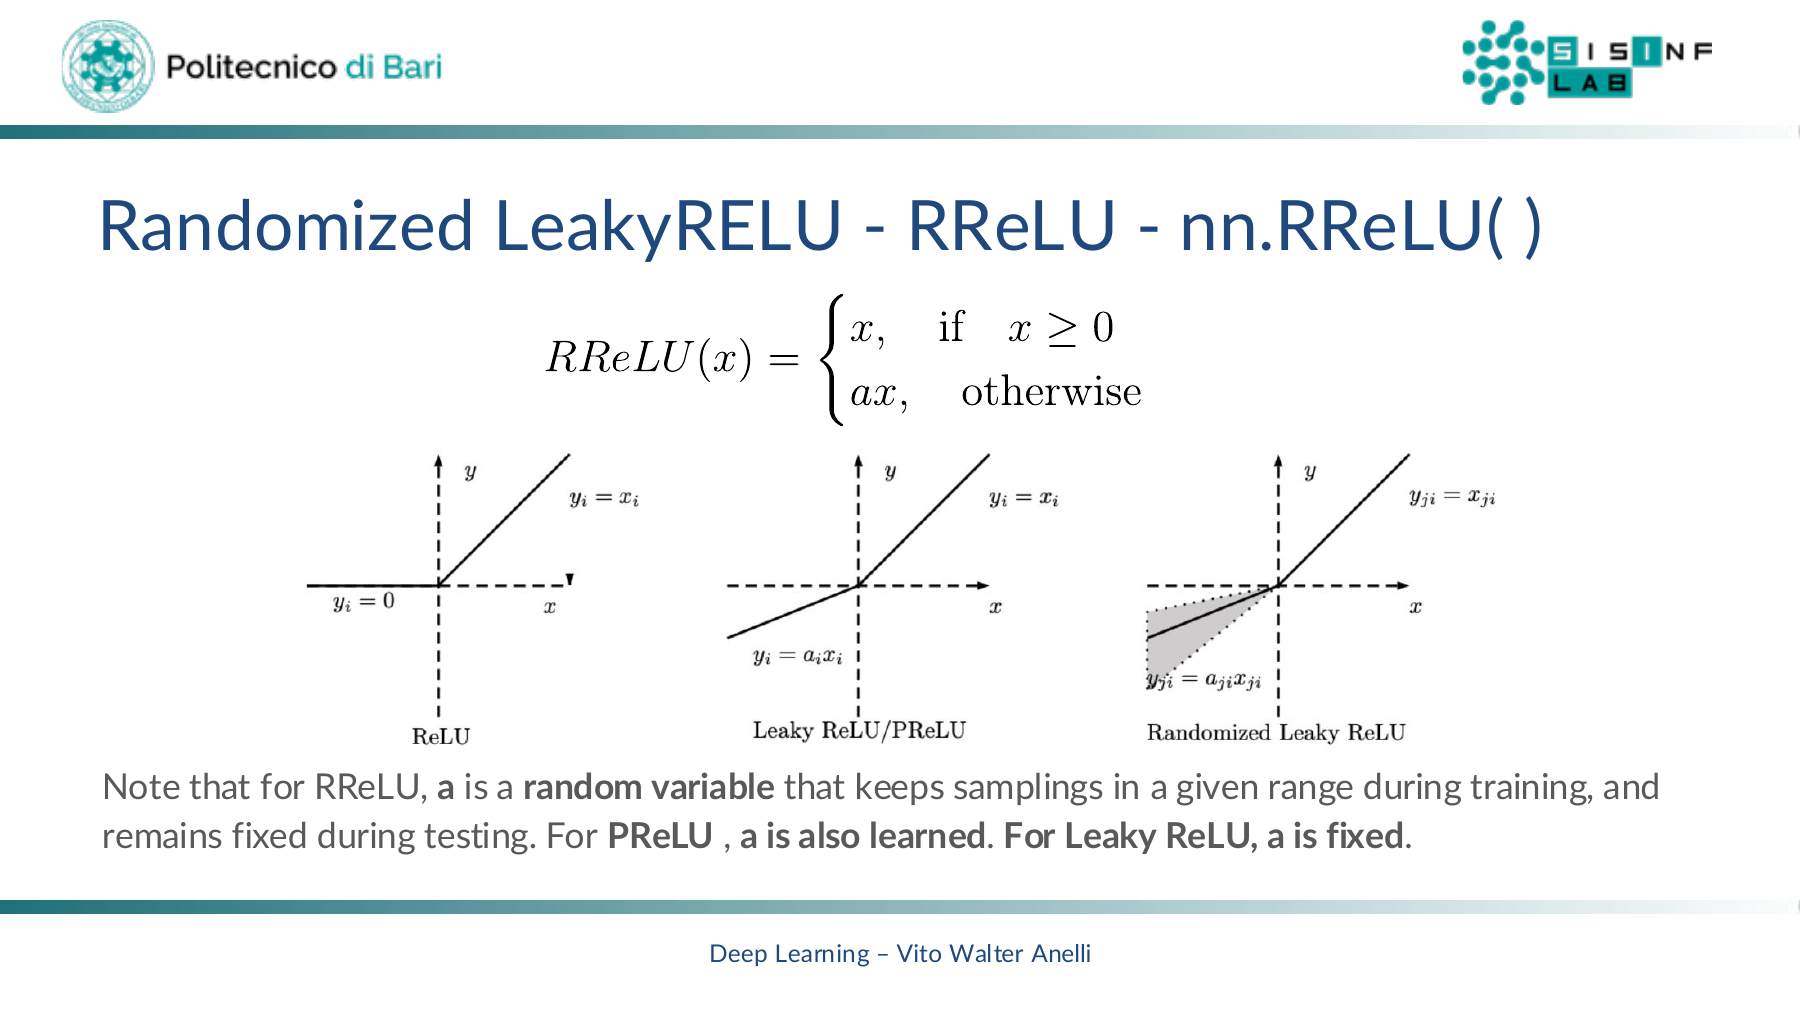
\includegraphics[width=0.85\linewidth]{figures/af03_rrelu.png}
  \caption{Confronto visivo tra ReLU, Leaky ReLU/PReLU e Randomized Leaky ReLU (RReLU).
           In RReLU, il parametro $a_{ji}$ è campionato uniformemente da un intervallo
           $[l,u]$ durante il training; al test viene usato il valor medio $(l+u)/2$.
           Questo effetto di randomizzazione funge da regolarizzazione implicita.}
  \label{fig:rrelu}
\end{figure}

\begin{figure}[H]
  \centering
  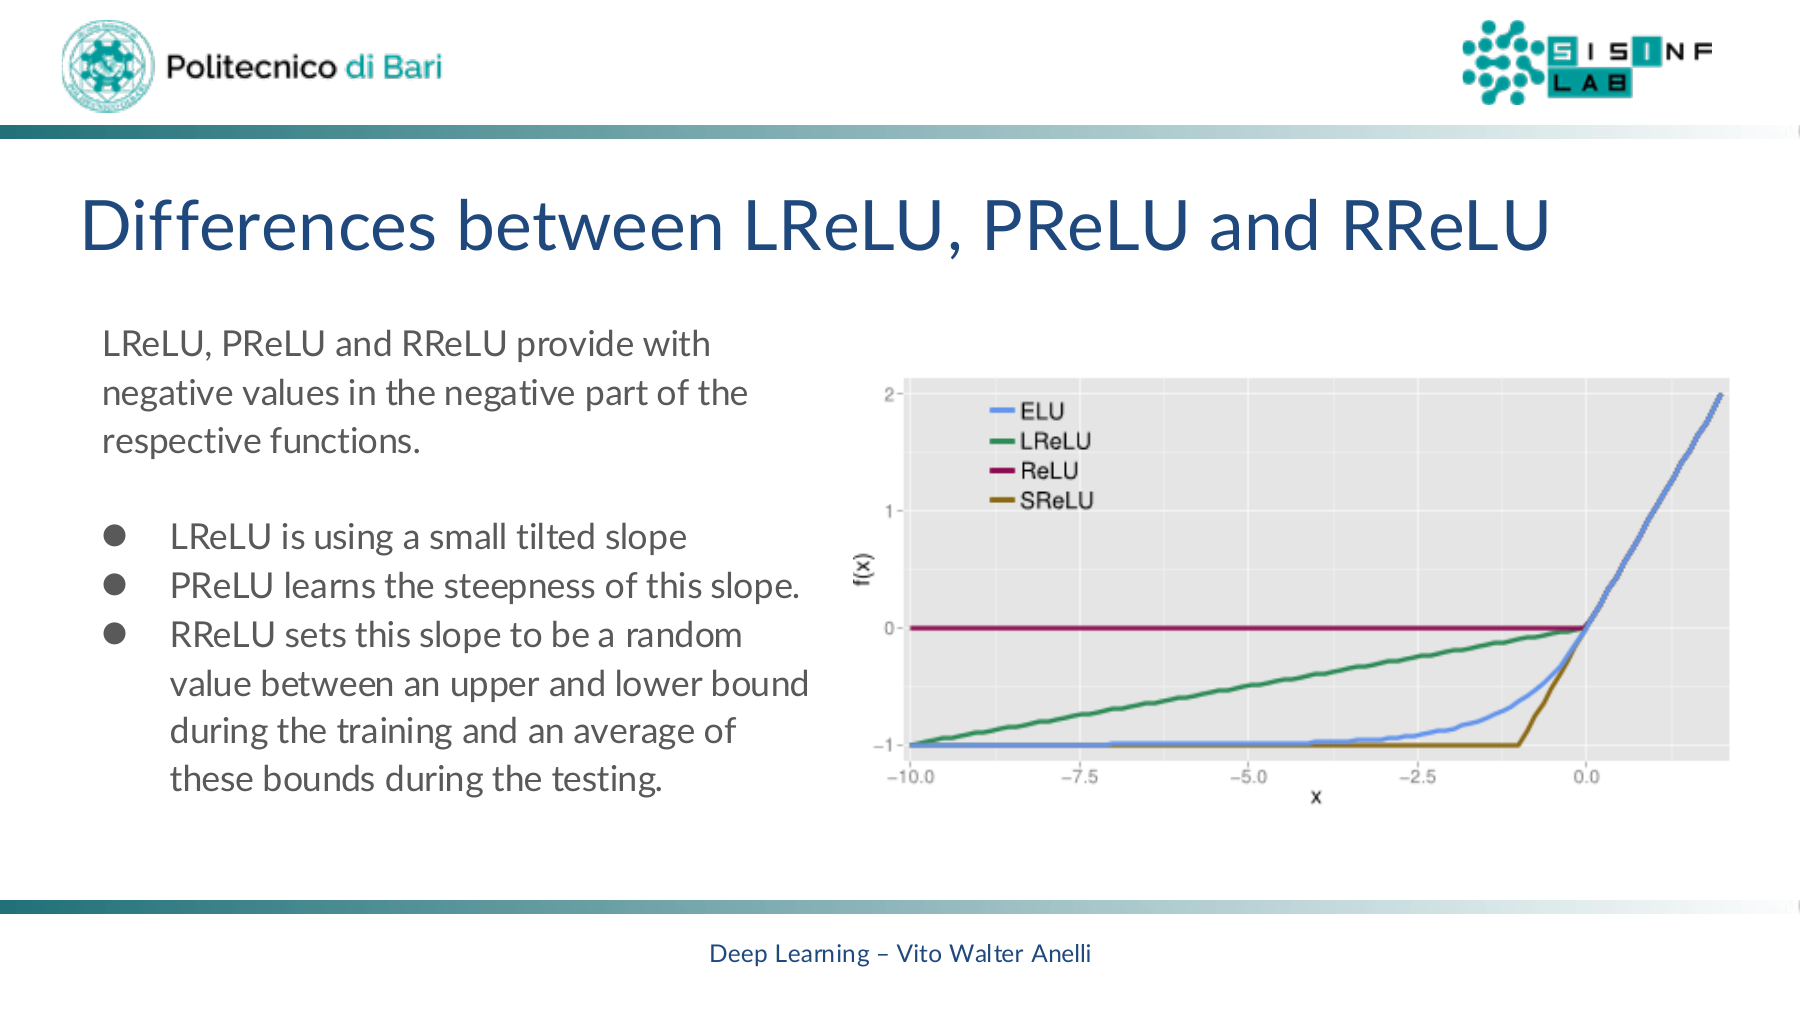
\includegraphics[width=0.80\linewidth]{figures/af03_lrelu_prelu_rrelu_diff.png}
  \caption{Differenze nella regione negativa tra ELU, LReLU, ReLU e SReLU.
           LReLU usa una pendenza fissa piccola; PReLU la apprende; RReLU
           la randomizza durante il training e la fissa alla media al test.}
  \label{fig:lrelu_prelu_rrelu_diff}
\end{figure}

\subsection{ReLU6 -- \texttt{nn.ReLU6()}}
\label{subsec:relu6}

\begin{equation}
  \operatorname{ReLU6}(x) = \min\!\bigl(\max(0, x),\, 6\bigr).
\end{equation}

\begin{figure}[H]
  \centering
  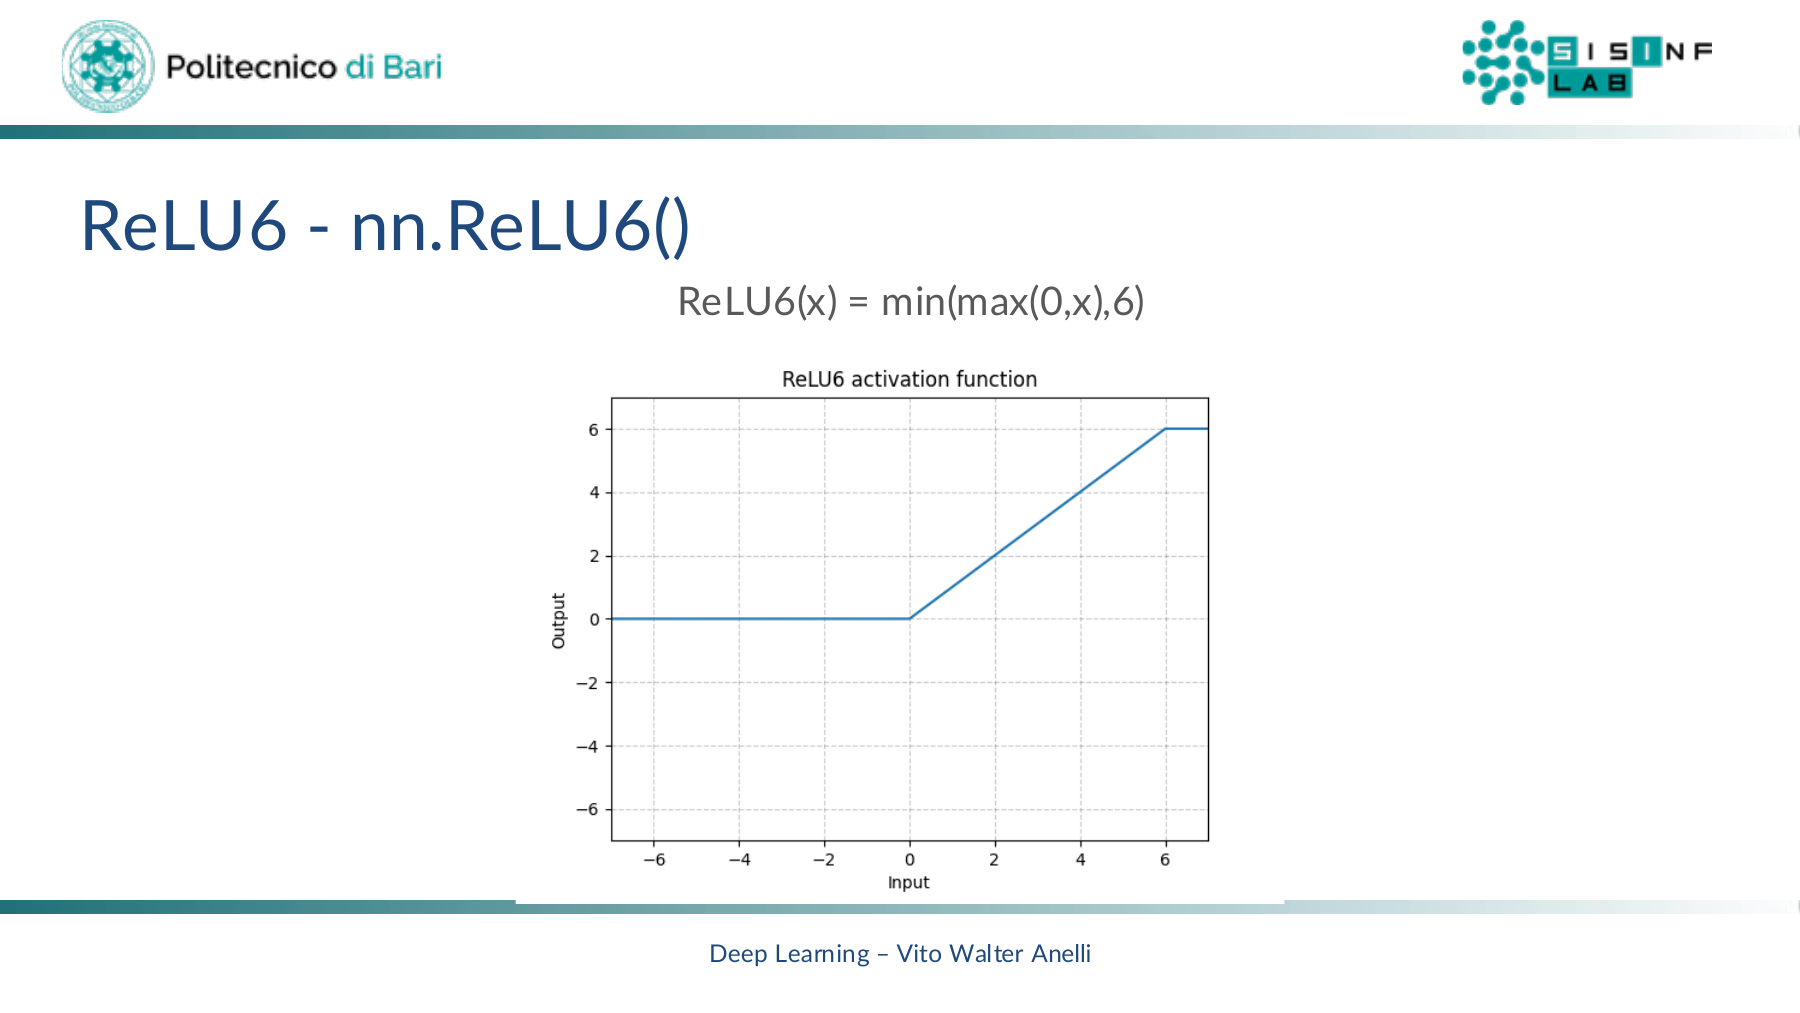
\includegraphics[width=0.72\linewidth]{figures/af03_relu6.png}
  \caption{ReLU6: ReLU con saturazione superiore a $6$. Progettata
           per ambienti a precisione ridotta (es.\ mobile/quantizzazione),
           previene attivazioni molto grandi che possono degradare la
           rappresentazione in virgola mobile a bassa precisione.}
  \label{fig:relu6}
\end{figure}

%------------------------------------------------------------
\section{Famiglia ELU}
\label{sec:elu-family}

\subsection{ELU -- \texttt{nn.ELU()}}
\label{subsec:elu}

La \textbf{Exponential Linear Unit} risolve sia il dead neuron problem sia il
problema delle medie non centrate in zero \citep{bishop2024}:

\begin{equation}
  \operatorname{ELU}(x) = \max(0,x) + \min\!\bigl(0,\, \alpha\cdot(\exp(x)-1)\bigr).
\end{equation}

\begin{figure}[H]
  \centering
  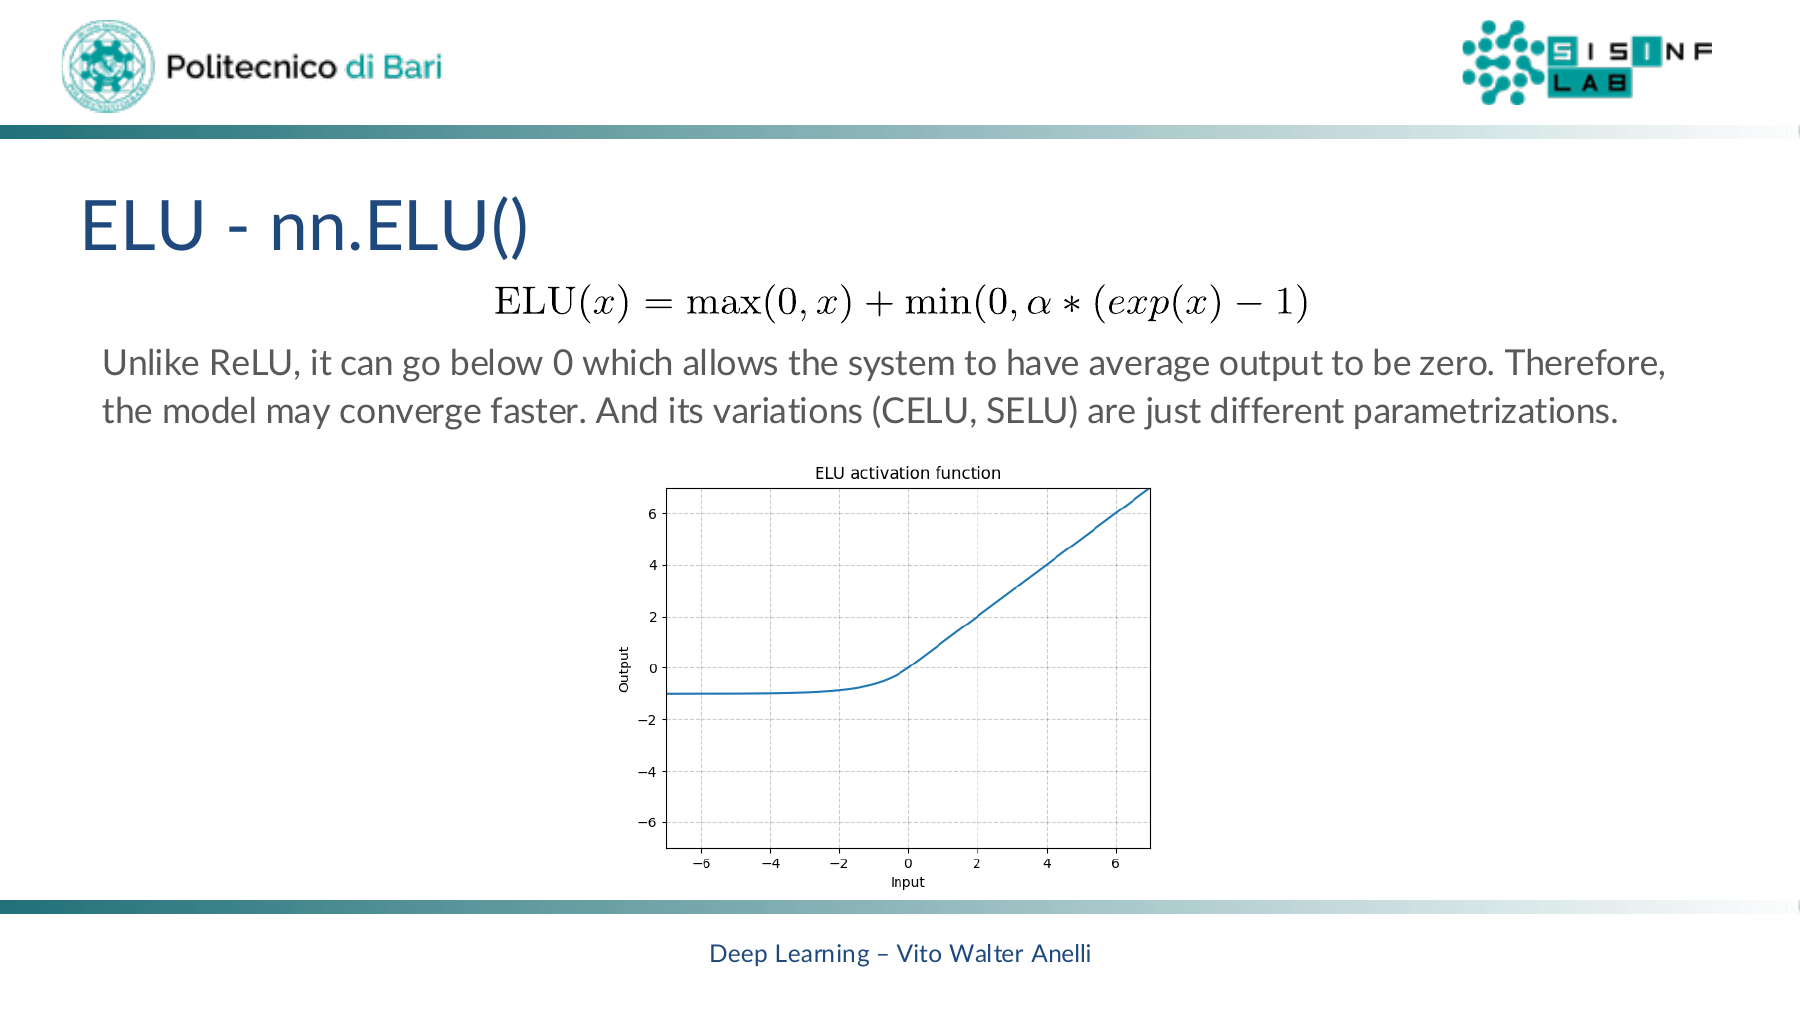
\includegraphics[width=0.72\linewidth]{figures/af03_elu.png}
  \caption{ELU: a differenza di ReLU, può produrre valori negativi,
           permettendo all'output medio del layer di essere vicino a zero.
           Questo centra le attivazioni e accelera la convergenza.
           Le varianti CELU e SELU sono reparametrizzazioni di ELU.}
  \label{fig:elu}
\end{figure}

Il valore $\alpha$ controlla il limite inferiore della regione negativa
(di default $\alpha = 1$). Avere output con media vicina a zero ha lo stesso
beneficio del \emph{Batch Normalization}: il gradiente non è sistematicamente
distorto, e la convergenza è più rapida.

\subsection{CELU -- \texttt{nn.CELU()}}
\label{subsec:celu}

\begin{equation}
  \operatorname{CELU}(x) = \max(0,x) + \min\!\left(0,\, \alpha \cdot
  \left(\exp\!\left(\frac{x}{\alpha}\right) - 1\right)\right).
\end{equation}

\begin{figure}[H]
  \centering
  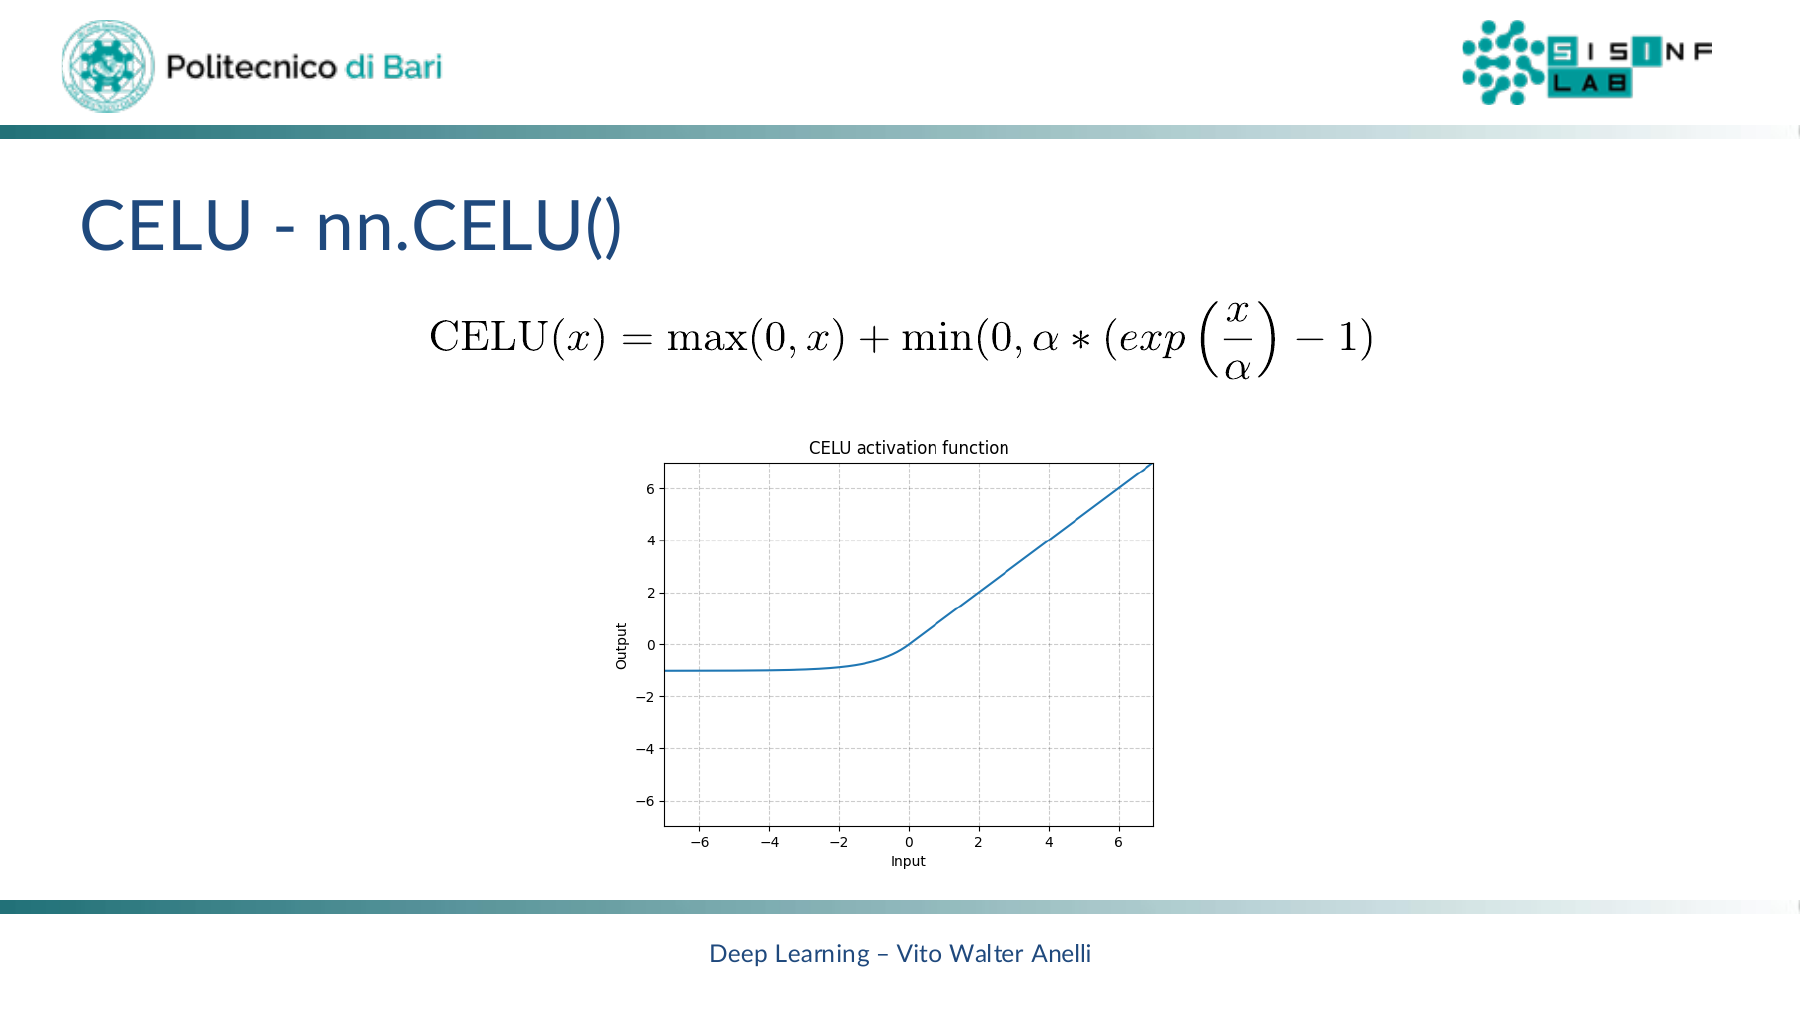
\includegraphics[width=0.72\linewidth]{figures/af03_celu.png}
  \caption{CELU (Continuously Differentiable ELU): reparametrizza ELU in modo
           da garantire la derivabilità continua in $x=0$ per qualsiasi valore
           di $\alpha$, migliorando la stabilità numerica del training.}
  \label{fig:celu}
\end{figure}

\subsection{SELU -- \texttt{nn.SELU()}}
\label{subsec:selu}

\begin{equation}
  \operatorname{SELU}(x) = \mathrm{scale} \cdot
  \bigl(\max(0,x) + \min\!\bigl(0,\,\alpha\cdot(\exp(x)-1)\bigr)\bigr),
\end{equation}
con $\mathrm{scale} \approx 1{,}0507$ e $\alpha \approx 1{,}6733$
(valori calcolati analiticamente da Klambauer et al., 2017).

\begin{figure}[H]
  \centering
  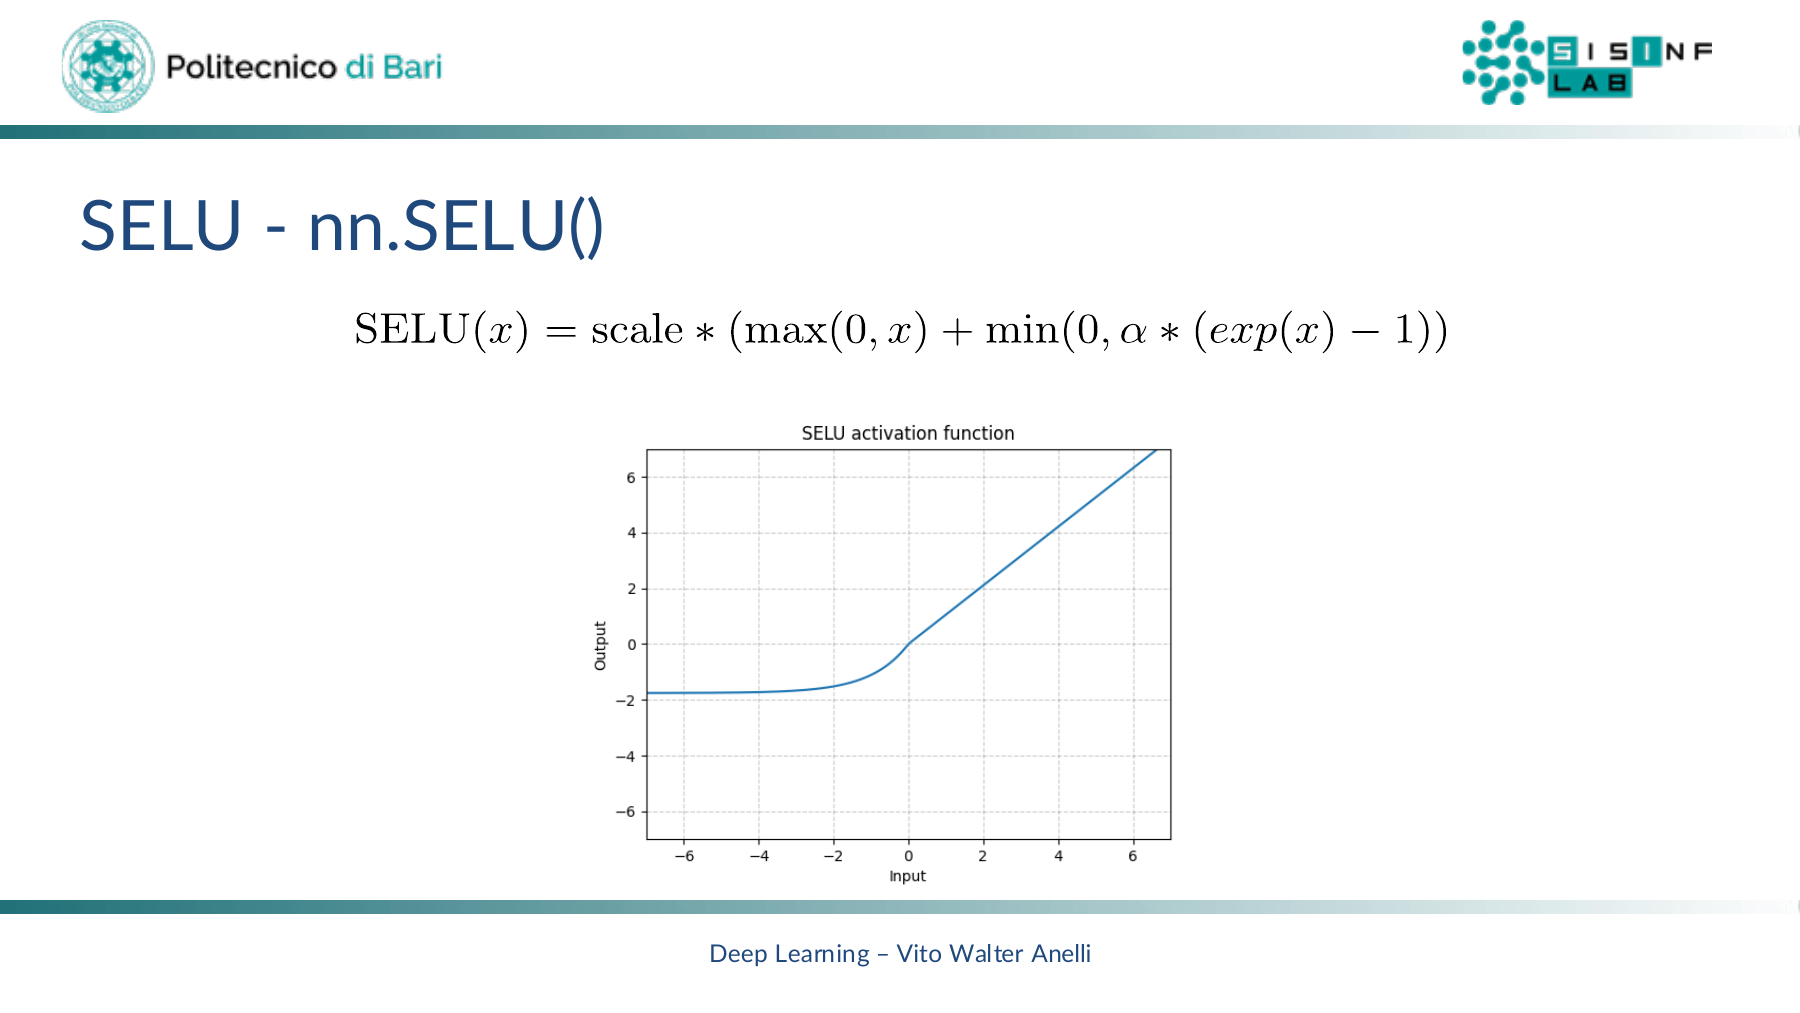
\includegraphics[width=0.72\linewidth]{figures/af03_selu.png}
  \caption{SELU (Scaled ELU): aggiunge un fattore di scala alla ELU.
           Con le costanti $\alpha$ e \emph{scale} opportune, la SELU garantisce
           \emph{self-normalizing} properties: attivazioni con media $0$ e
           varianza $1$ si propagano stabili attraverso layer arbitrariamente
           profondi, senza necessità di Batch Normalization.}
  \label{fig:selu}
\end{figure}

%------------------------------------------------------------
\section{Softplus e GELU}
\label{sec:softplus-gelu}

\subsection{Softplus -- \texttt{nn.Softplus()}}
\label{subsec:softplus}

\begin{equation}
  \operatorname{Softplus}(x) = \frac{1}{\beta} \cdot \log\!\bigl(1 + \exp(\beta x)\bigr).
\end{equation}

\begin{figure}[H]
  \centering
  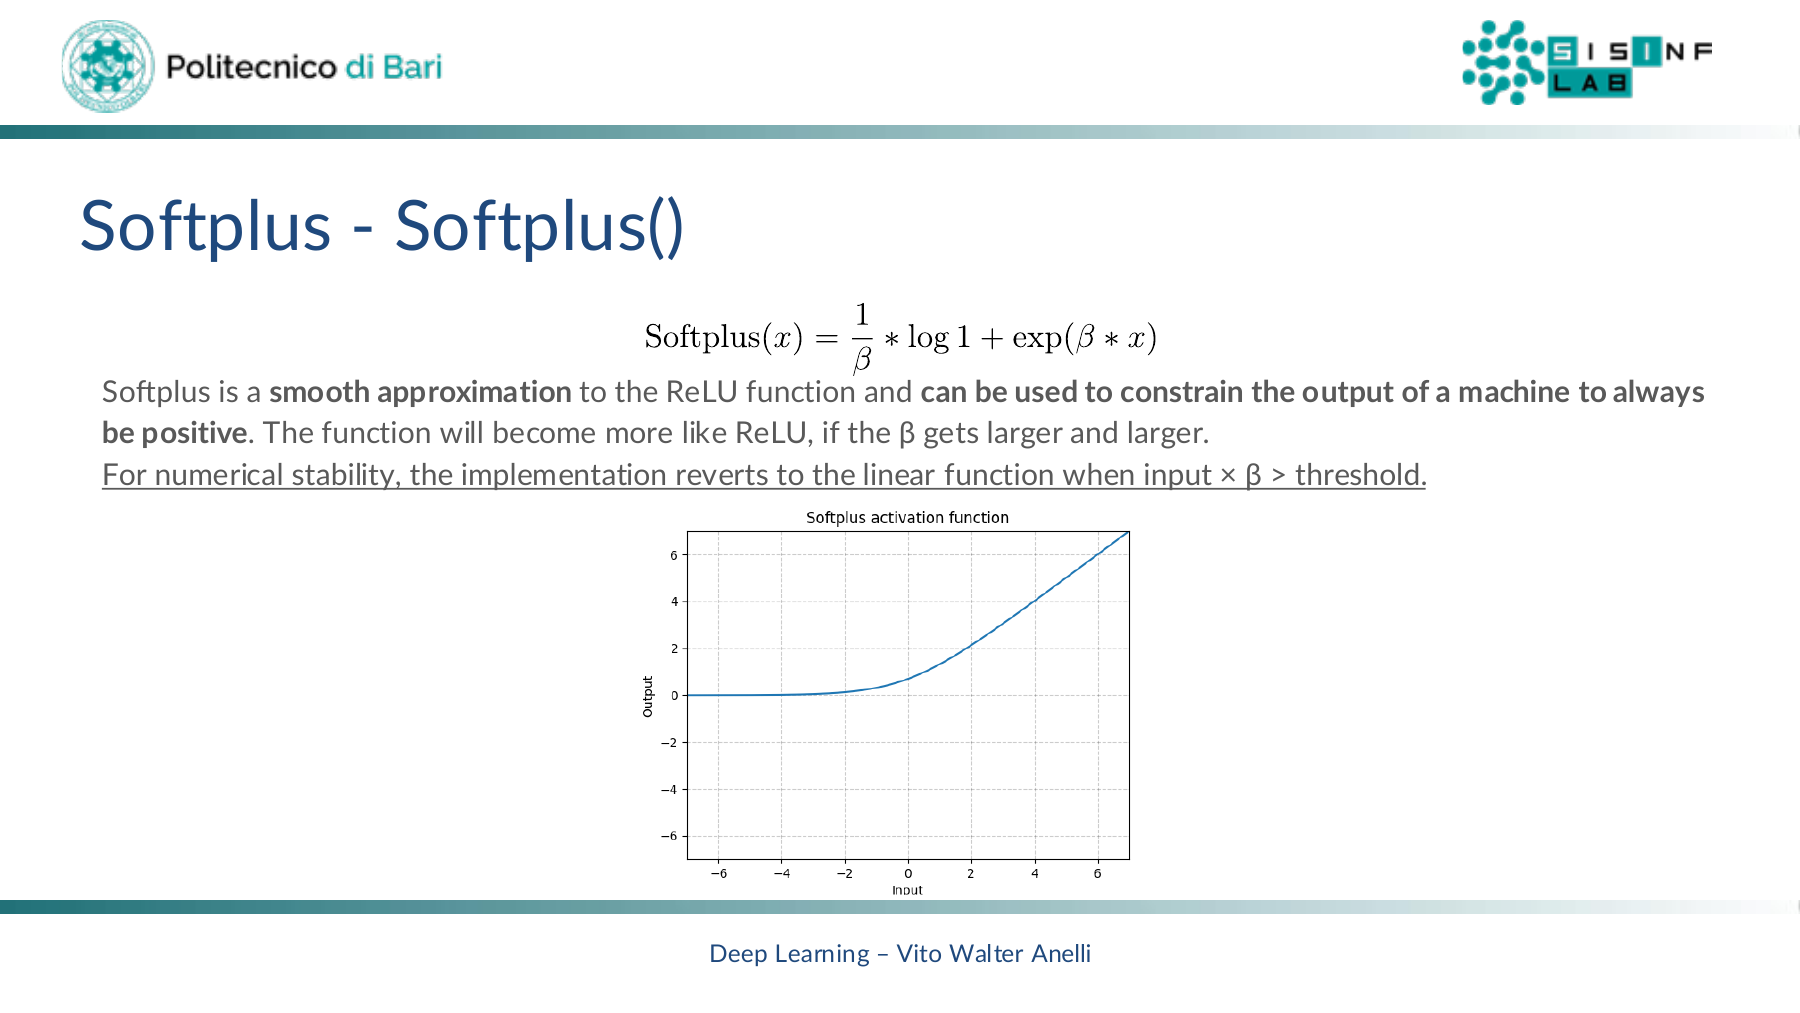
\includegraphics[width=0.72\linewidth]{figures/af03_softplus.png}
  \caption{Softplus: approssimazione \textbf{smooth} di ReLU, con derivata continua
           in tutto $\mathbb{R}$. All'aumentare di $\beta$ converge a ReLU.
           Può essere usata per \emph{vincolare l'output a essere sempre positivo}.
           Per stabilità numerica, l'implementazione torna alla funzione lineare
           quando $x \cdot \beta > \mathrm{threshold}$.}
  \label{fig:softplus}
\end{figure}

La Softplus è la primitiva della Sigmoid: $\frac{d}{dx}\operatorname{Softplus}(x) = \sigma(x)$,
il che ne chiarisce il ruolo teorico come ``versione continua'' di ReLU.

\subsection{GELU -- \texttt{nn.GELU()}}
\label{subsec:gelu}

\begin{equation}
  \operatorname{GELU}(x) = x \cdot \Phi(x),
\end{equation}
dove $\Phi(x)$ è la \emph{Cumulative Distribution Function} della distribuzione gaussiana standard.

\begin{figure}[H]
  \centering
  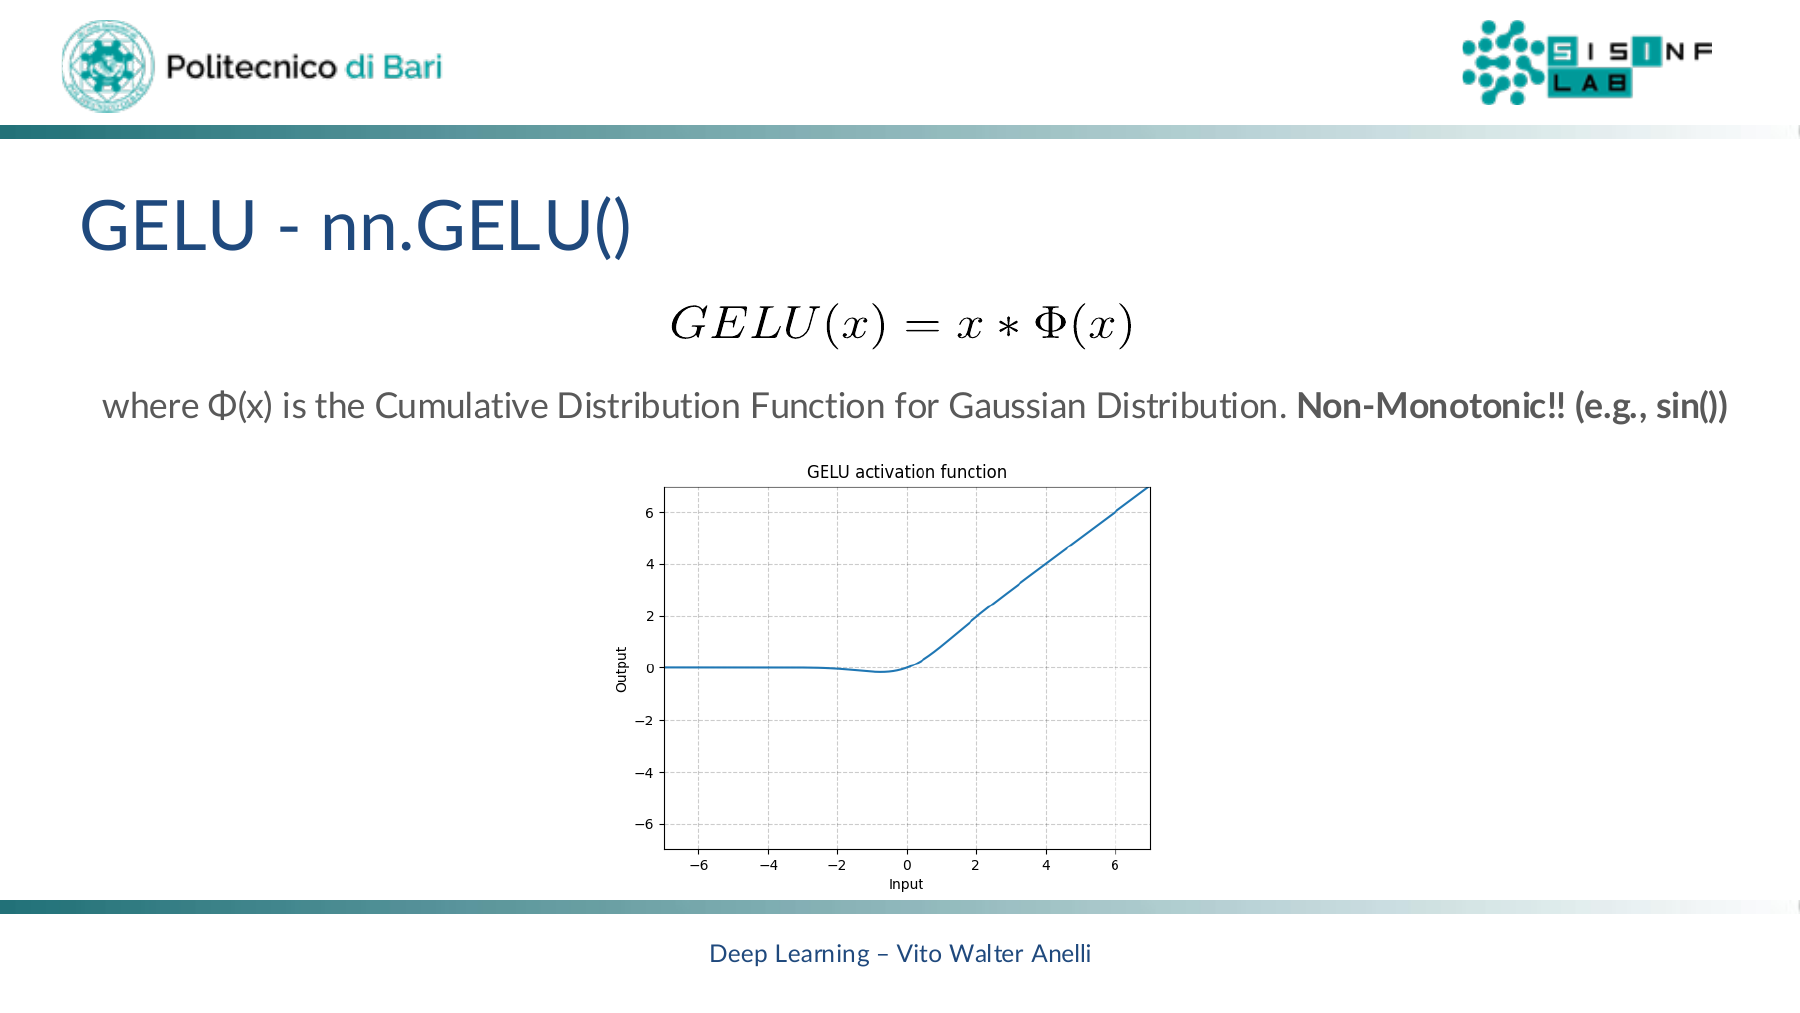
\includegraphics[width=0.72\linewidth]{figures/af03_gelu.png}
  \caption{GELU (Gaussian Error Linear Unit): funzione \textbf{non monotona},
           a differenza di ReLU e delle sue varianti. Nella regione $x < 0$
           l'output decresce, poi risale, imitando il comportamento del dropout
           stocastico. È la funzione di attivazione predefinita nei Transformer
           (BERT, GPT) per le sue proprietà di regolarizzazione implicita.}
  \label{fig:gelu}
\end{figure}

L'approssimazione pratica spesso utilizzata è:
\begin{equation}
  \operatorname{GELU}(x) \approx 0{,}5\, x
  \left(1 + \tanh\!\left[\sqrt{\frac{2}{\pi}}\bigl(x + 0{,}044715\, x^3\bigr)\right]\right).
\end{equation}

%------------------------------------------------------------
\section{Funzioni Saturanti}
\label{sec:saturating}

\subsection{Sigmoid -- \texttt{nn.Sigmoid()}}
\label{subsec:sigmoid}

\begin{equation}
  \operatorname{Sigmoid}(x) = \sigma(x) = \frac{1}{1 + \exp(-x)}.
\end{equation}

\begin{figure}[H]
  \centering
  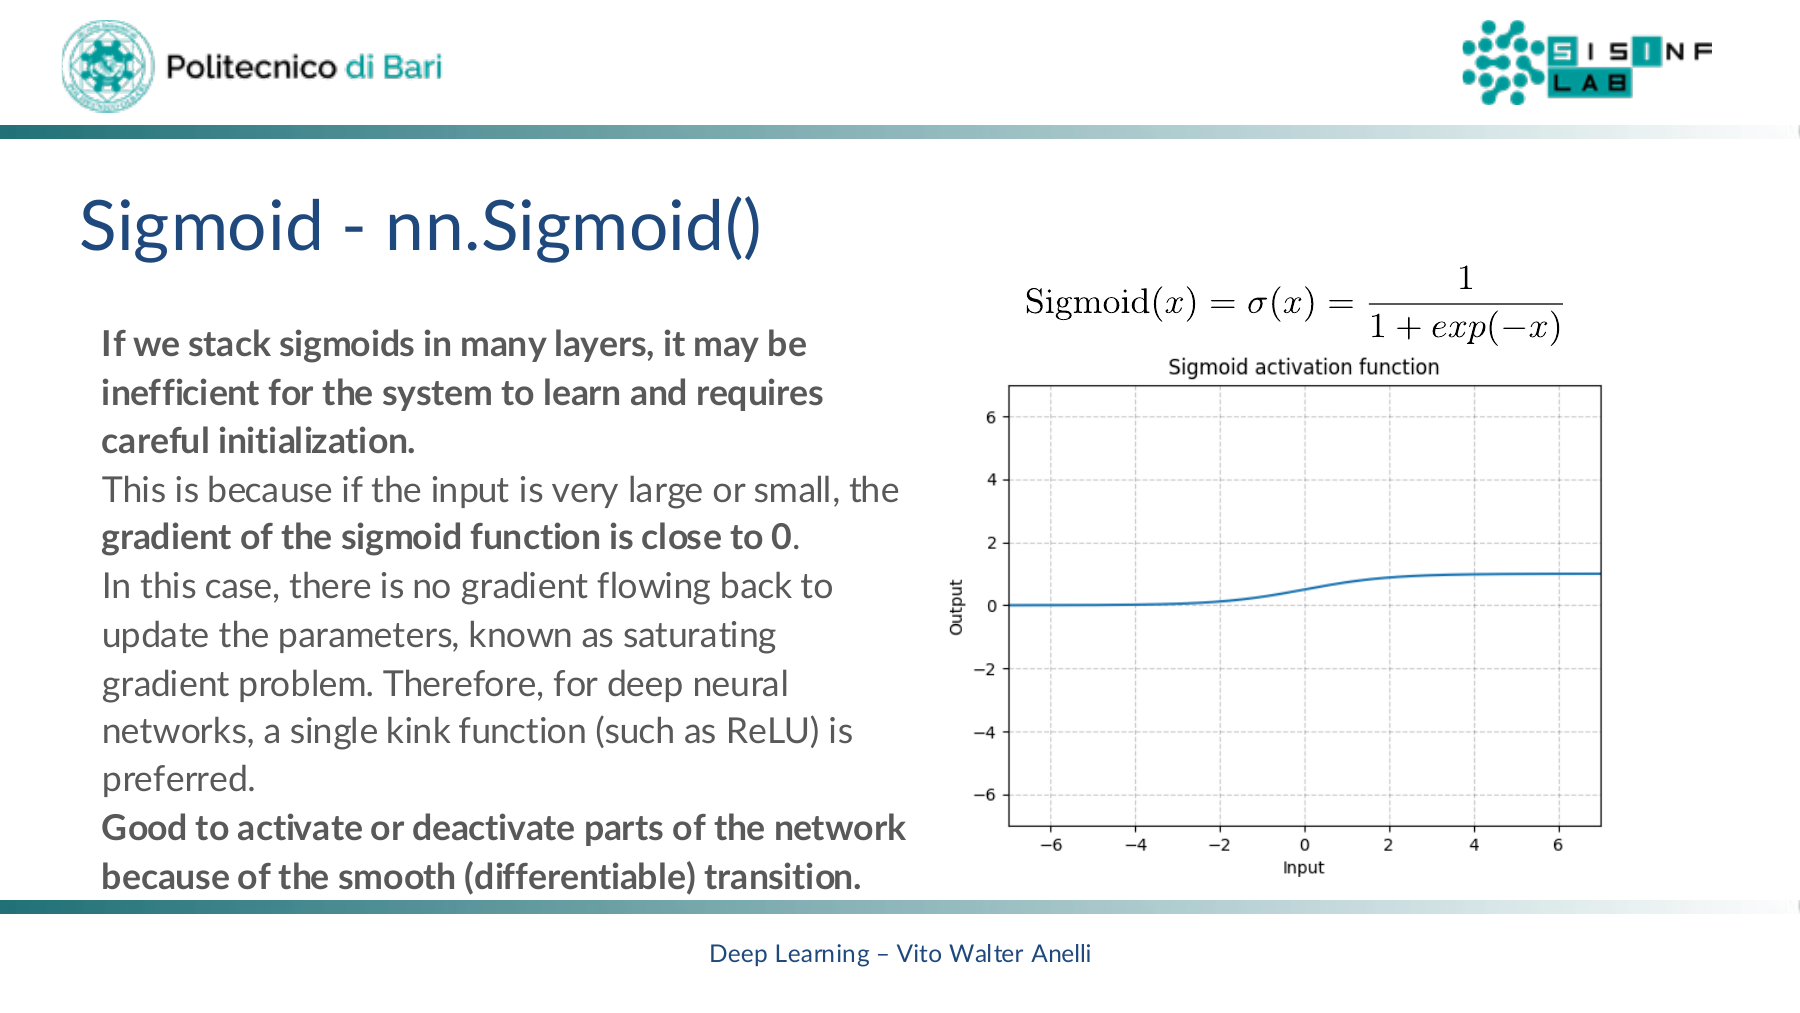
\includegraphics[width=0.85\linewidth]{figures/af03_sigmoid.png}
  \caption{Sigmoid: output in $(0,1)$, il che la rende ideale come gate
           (LSTM, GRU) o per output probabilistici di classificatori binari.
           Impilare molti layer sigmoid causa il vanishing gradient: il gradiente
           della sigmoid è prossimo a zero per $|x| \gg 0$, bloccando la
           retropropagazione. Per reti profonde si preferisce ReLU.}
  \label{fig:sigmoid}
\end{figure}

\paragraph{Connessione con Softmax.}
Come mostrato nelle slide (Sez.~\ref{sec:softmax}), la Sigmoid è un caso
speciale della Softmax a due classi: posto $x_2 = 0$,
\begin{equation}
  z_1 = \frac{e^{x_1}}{e^{x_1}+e^{x_2}}
      = \frac{e^{x_1}}{e^{x_1}+1}
      = \frac{1}{1+e^{-x_1}} = \sigma(x_1).
\end{equation}

\subsection{Tanh -- \texttt{nn.Tanh()}}
\label{subsec:tanh}

\begin{equation}
  \operatorname{Tanh}(x) = \tanh(x) = \frac{\exp(x) - \exp(-x)}{\exp(x) + \exp(-x)}.
\end{equation}

\begin{figure}[H]
  \centering
  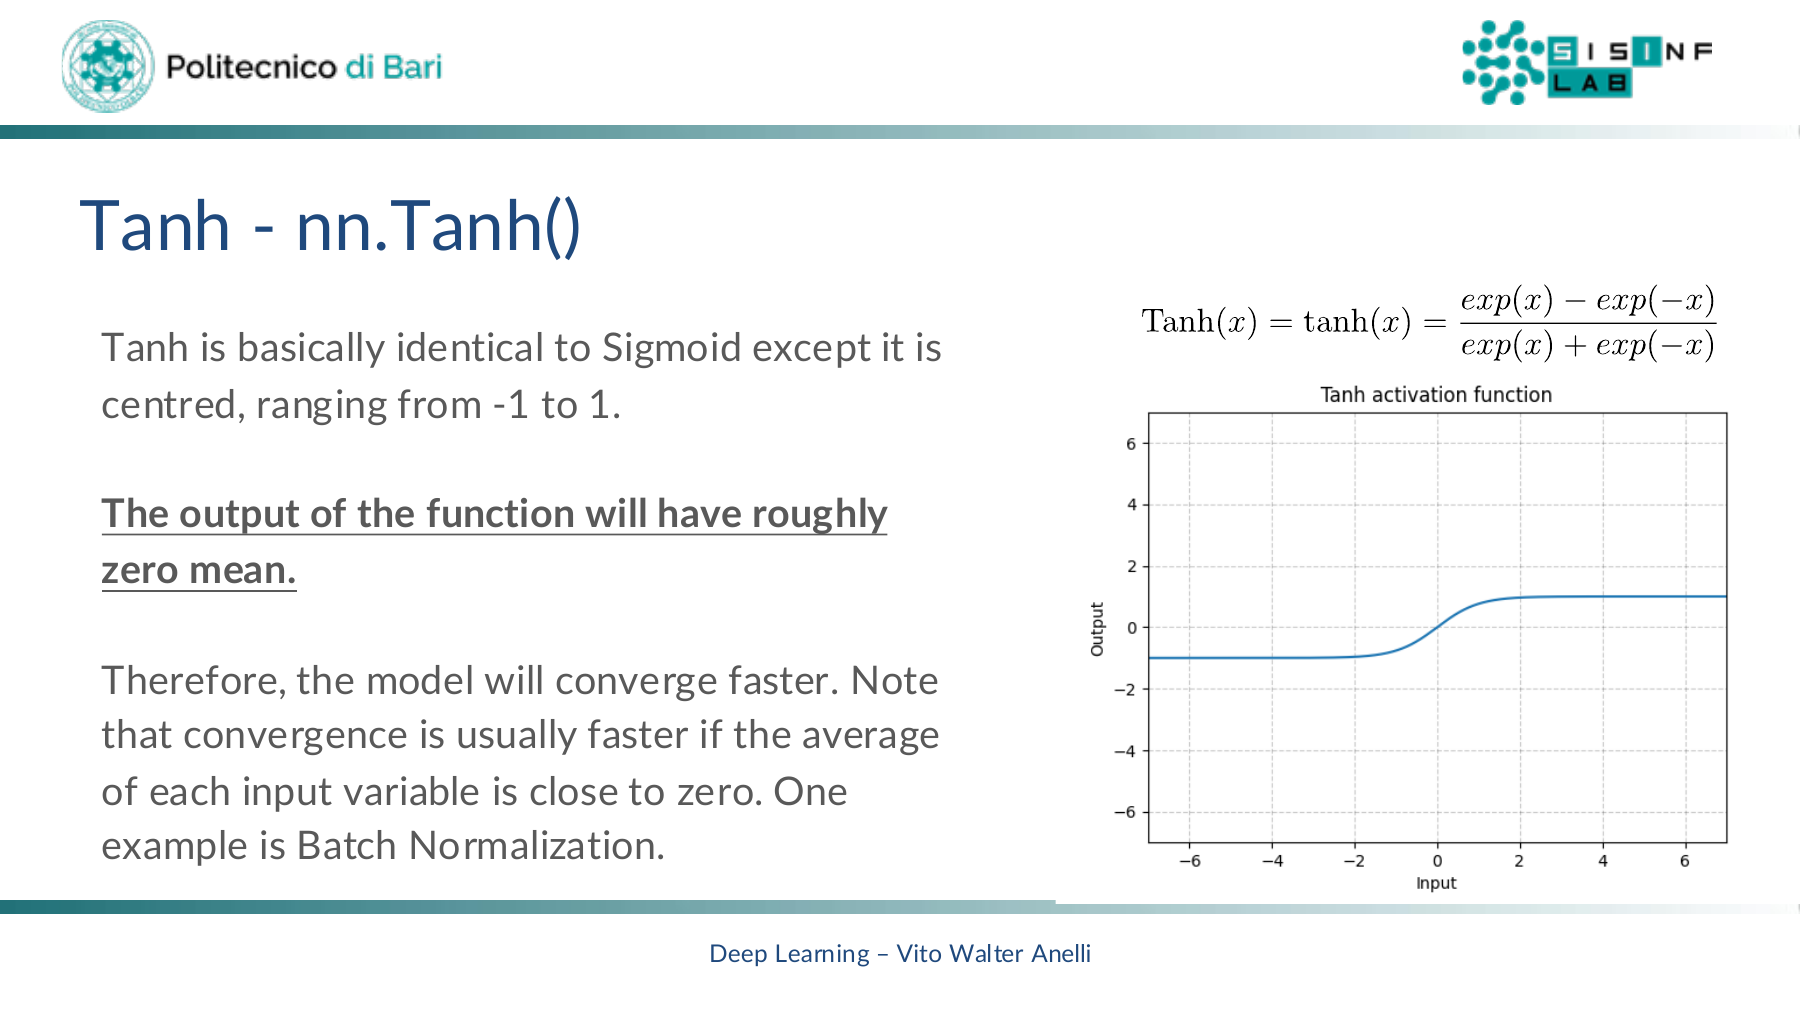
\includegraphics[width=0.85\linewidth]{figures/af03_tanh.png}
  \caption{Tanh: versione centrata della Sigmoid con output in $(-1, 1)$.
           L'output ha media approssimativamente zero, accelerando la convergenza
           rispetto a Sigmoid (nota fondamentale: la convergenza è più rapida
           quando la media degli input è vicina a zero, come avviene nel
           Batch Normalization). Soffre comunque del vanishing gradient.}
  \label{fig:tanh}
\end{figure}

\paragraph{Relazione con Sigmoid.}
$\tanh(x) = 2\sigma(2x) - 1$: Tanh è semplicemente una Sigmoid riscalata e
traslata. Preferire Tanh a Sigmoid nei layer nascosti perché l'output centrato
evita bias sistematici nel gradiente \citep{bishop2024}.

\subsection{Hardtanh -- \texttt{nn.Hardtanh()}}
\label{subsec:hardtanh}

\begin{equation}
  \operatorname{Hardtanh}(x) =
  \begin{cases}
    1,  & \text{se } x > 1 \\
    -1, & \text{se } x < -1 \\
    x,  & \text{altrimenti}
  \end{cases}
\end{equation}

\begin{figure}[H]
  \centering
  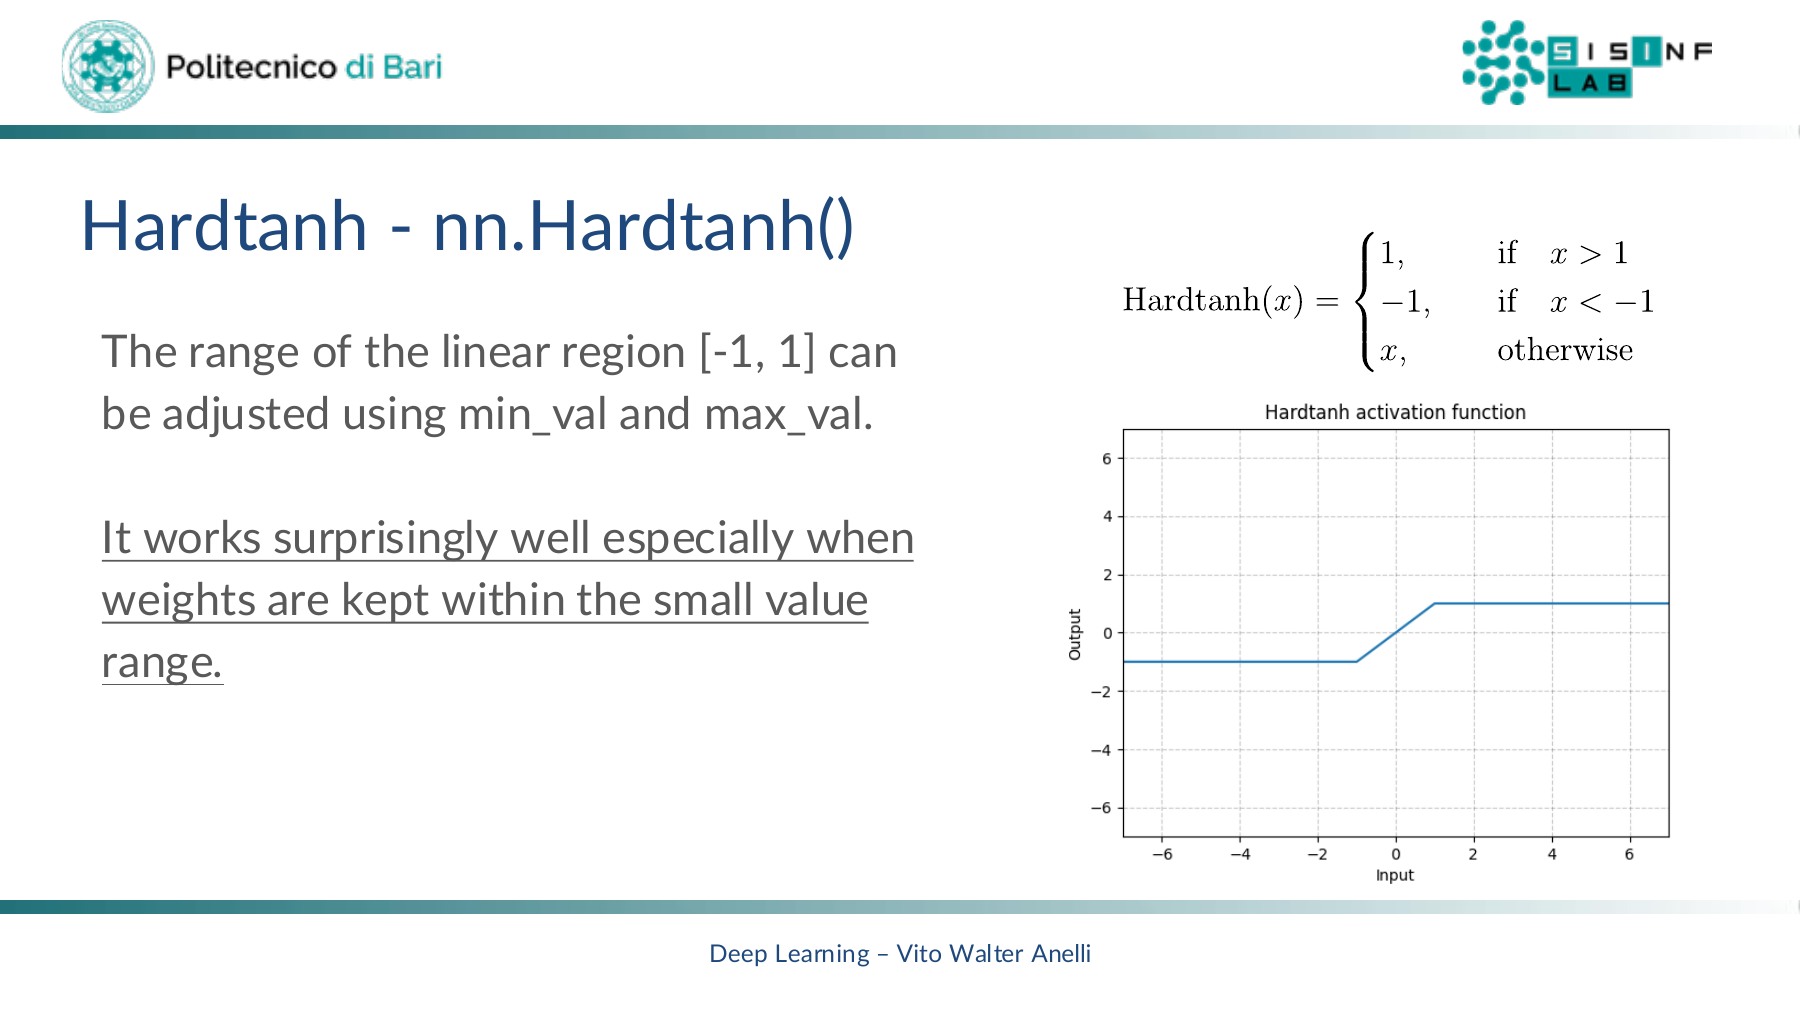
\includegraphics[width=0.85\linewidth]{figures/af03_hardtanh.png}
  \caption{Hardtanh: approssimazione lineare a tratti di Tanh.
           I valori di saturazione $[-1, 1]$ sono regolabili tramite
           \texttt{min\_val} e \texttt{max\_val}. Funziona sorprendentemente
           bene quando i pesi rimangono in un range di valori piccoli, ed è
           computazionalmente più leggera di Tanh.}
  \label{fig:hardtanh}
\end{figure}

\subsection{Softsign -- \texttt{nn.Softsign()}}
\label{subsec:softsign}

\begin{equation}
  \operatorname{SoftSign}(x) = \frac{x}{1 + |x|}.
\end{equation}

\begin{figure}[H]
  \centering
  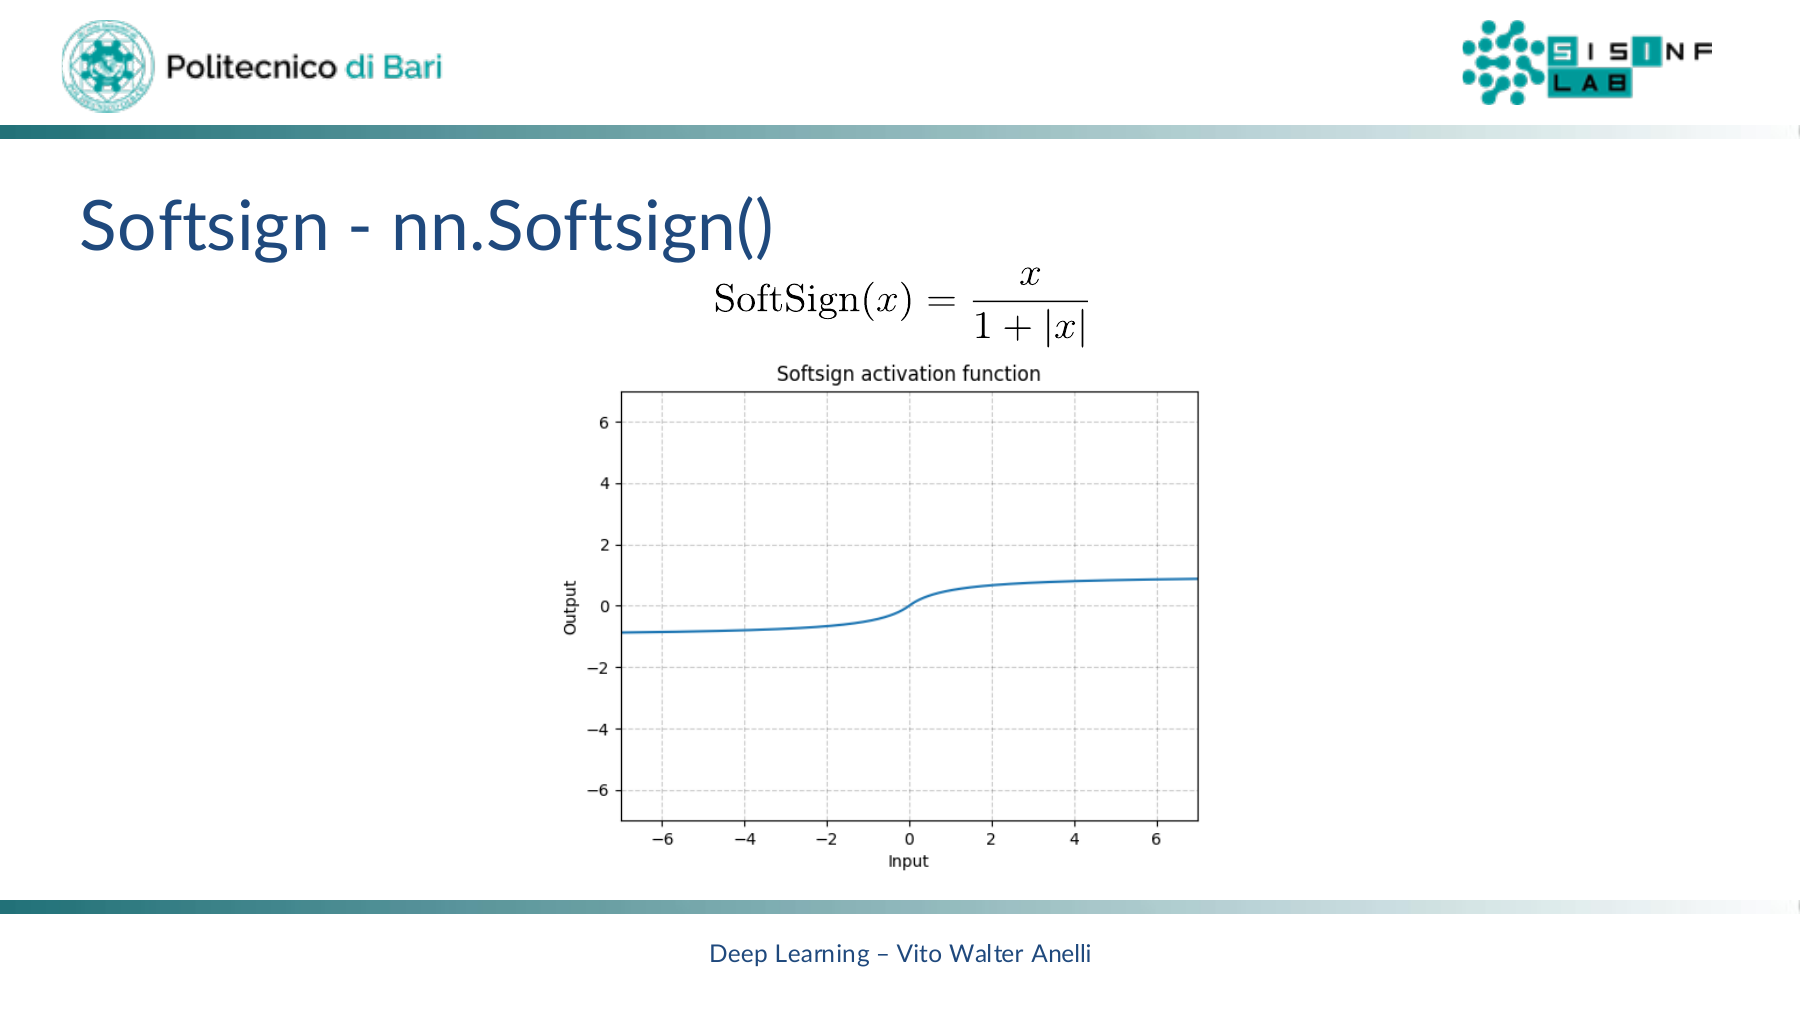
\includegraphics[width=0.72\linewidth]{figures/af03_softsign.png}
  \caption{Softsign: alternativa a Tanh con saturazione più lenta
           (decadimento polinomiale anziché esponenziale). Le code più
           pesanti implicano gradienti meno soggetti al vanishing problem
           rispetto a Tanh, ma l'output rimane in $(-1,1)$.}
  \label{fig:softsign}
\end{figure}

%------------------------------------------------------------
\section{Funzioni Shrink e Threshold}
\label{sec:shrink-threshold}

\subsection{Threshold -- \texttt{nn.Threshold()}}
\label{subsec:threshold}

\begin{equation}
  \operatorname{threshold}(x) =
  \begin{cases}
    x, & \text{se } x > \mathrm{threshold} \\
    v, & \text{altrimenti}
  \end{cases}
\end{equation}

\begin{figure}[H]
  \centering
  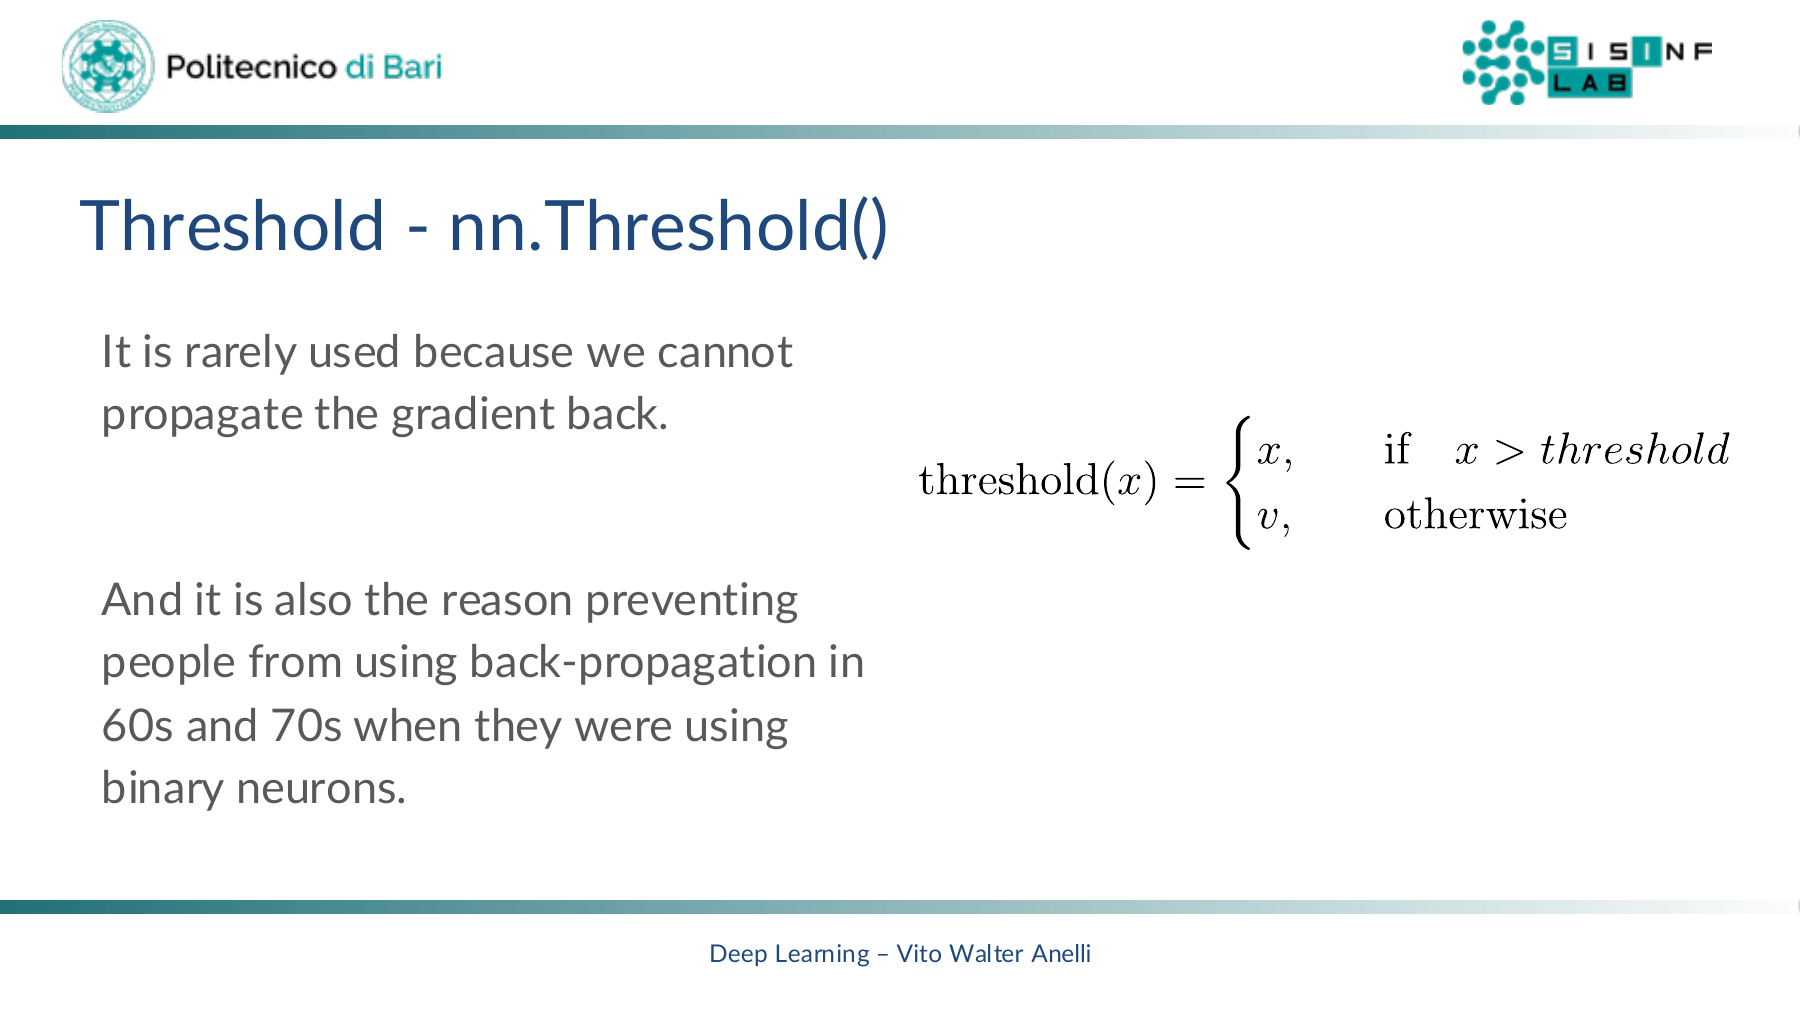
\includegraphics[width=0.72\linewidth]{figures/af03_threshold.png}
  \caption{Threshold (neurone binario): il gradiente è zero nella regione
           subthreshold, rendendo impossibile la retropropagazione per quei neuroni.
           È la ragione storica per cui la backpropagation non venne adottata
           negli anni '60--'70, quando si usavano neuroni binari.
           Attualmente non è utilizzata in reti moderne.}
  \label{fig:threshold}
\end{figure}

\subsection{Tanhshrink -- \texttt{nn.Tanhshrink()}}
\label{subsec:tanhshrink}

\begin{equation}
  \operatorname{Tanhshrink}(x) = x - \tanh(x).
\end{equation}

\begin{figure}[H]
  \centering
  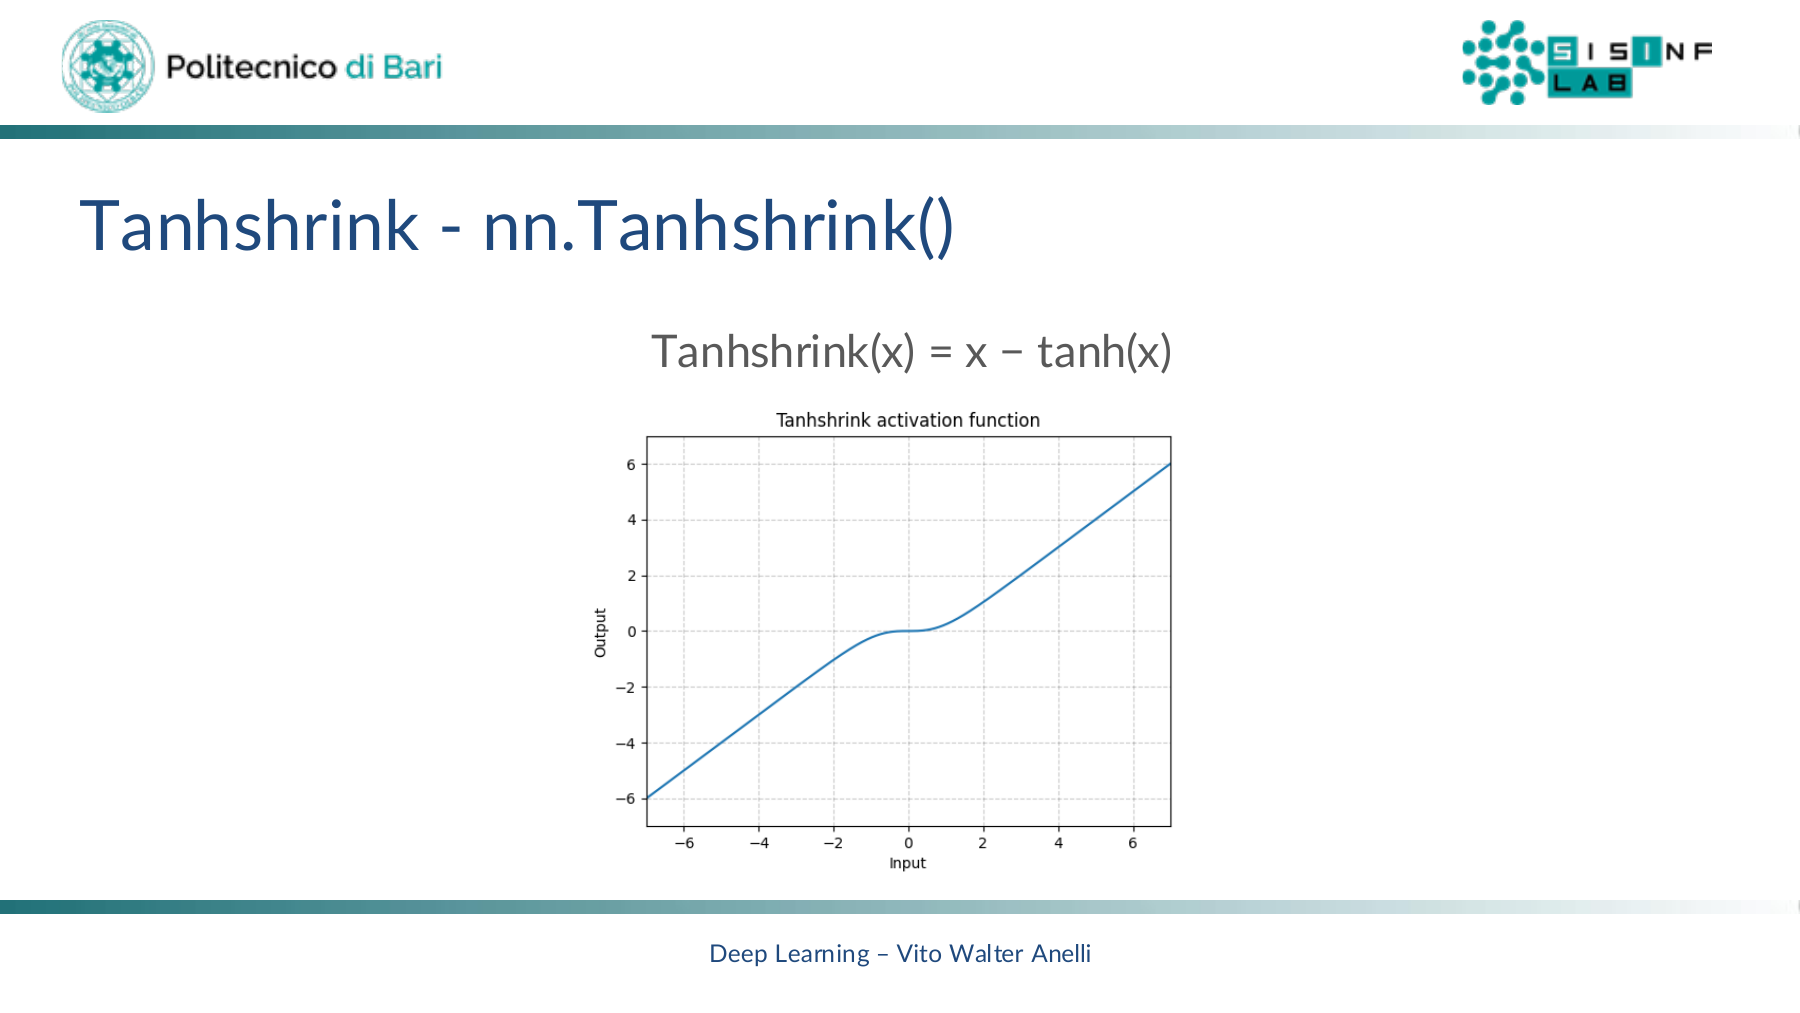
\includegraphics[width=0.72\linewidth]{figures/af03_tanhshrink.png}
  \caption{Tanhshrink: sottrae $\tanh(x)$ dall'input, producendo una funzione
           quasi lineare (con una lieve curvatura centrale). Usata in contesti
           di sparse coding per promuovere rappresentazioni sparse.}
  \label{fig:tanhshrink}
\end{figure}

\subsection{Softshrink -- \texttt{nn.Softshrink()}}
\label{subsec:softshrink}

\begin{equation}
  \operatorname{Softshrinkage}(x) =
  \begin{cases}
    x - \lambda, & \text{se } x > \lambda \\
    x + \lambda, & \text{se } x < -\lambda \\
    0,           & \text{altrimenti}
  \end{cases}
\end{equation}

\begin{figure}[H]
  \centering
  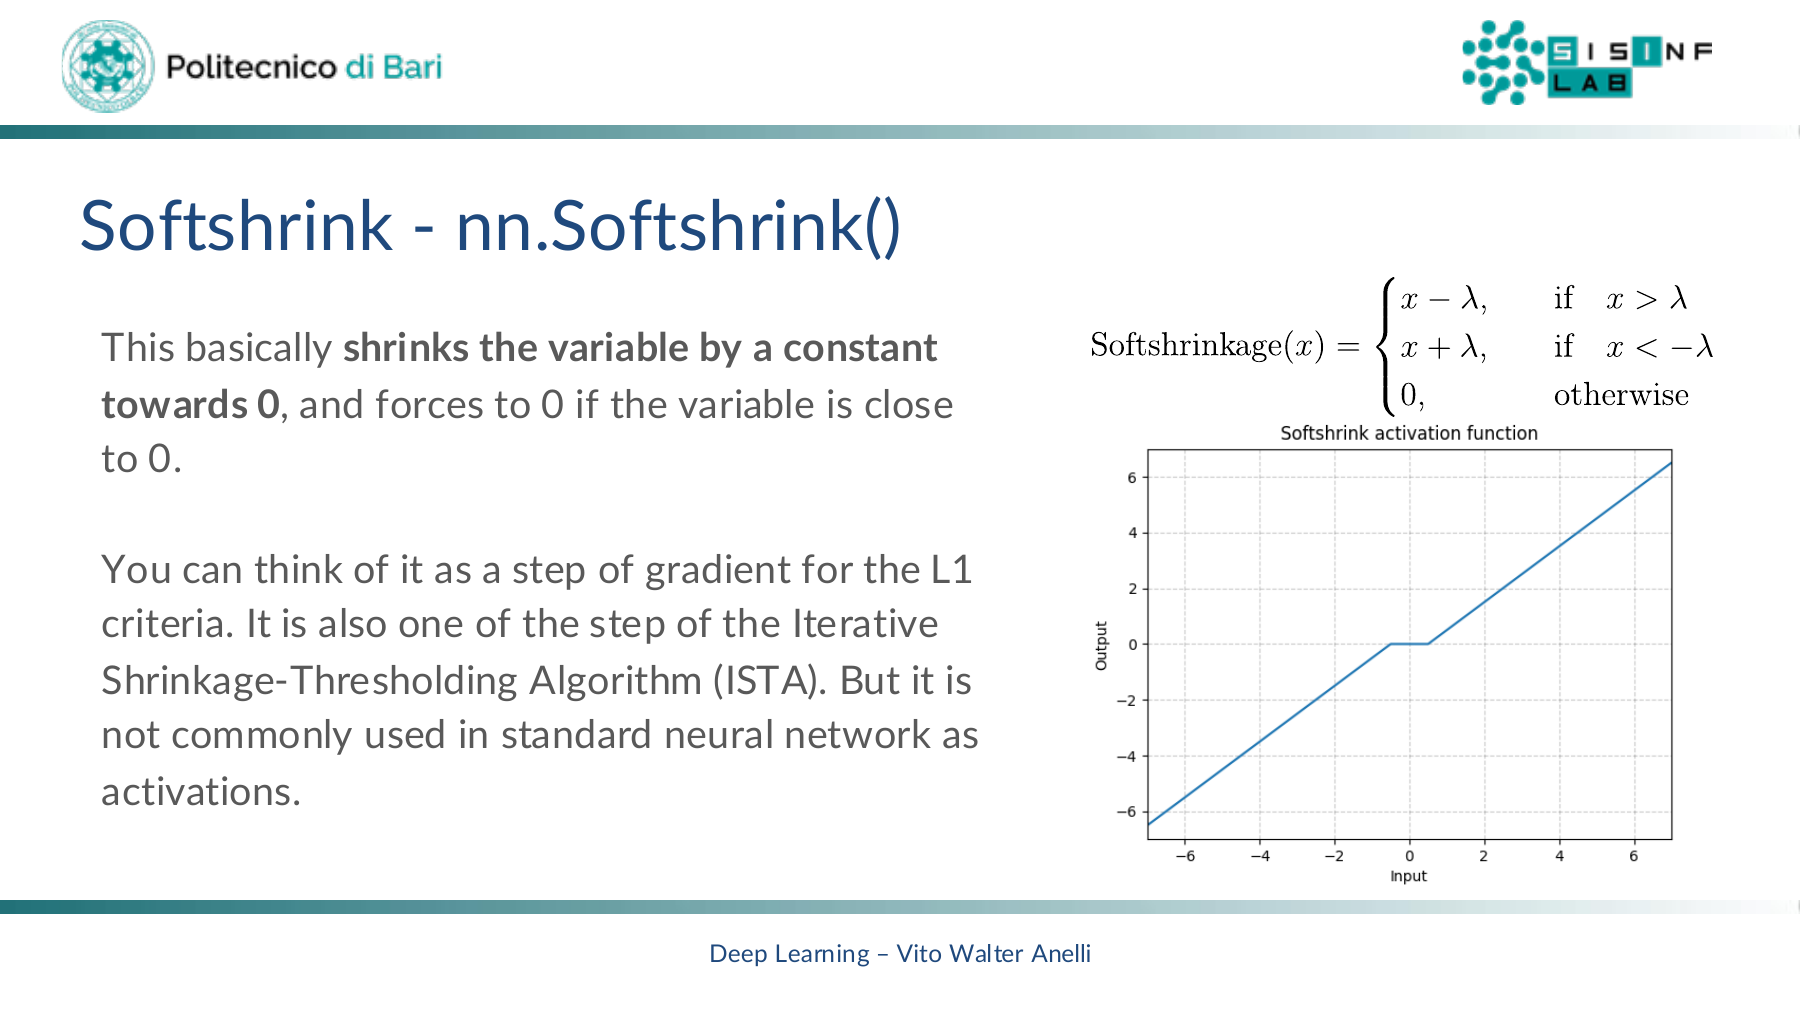
\includegraphics[width=0.85\linewidth]{figures/af03_softshrink.png}
  \caption{Softshrink: riduce il valore assoluto di $x$ di $\lambda$ verso zero,
           forzando a zero gli input nell'intervallo $[-\lambda, \lambda]$.
           Corrisponde a un passo del gradiente per la norma $L_1$ ed è
           uno step dell'algoritmo ISTA (\emph{Iterative Shrinkage-Thresholding}).
           Non è comunemente usata come attivazione nelle reti standard.}
  \label{fig:softshrink}
\end{figure}

\subsection{Hardshrink -- \texttt{nn.Hardshrink()}}
\label{subsec:hardshrink}

\begin{equation}
  \operatorname{Hardshrink}(x) =
  \begin{cases}
    x, & \text{se } x > \lambda \\
    x, & \text{se } x < -\lambda \\
    0, & \text{altrimenti}
  \end{cases}
\end{equation}

\begin{figure}[H]
  \centering
  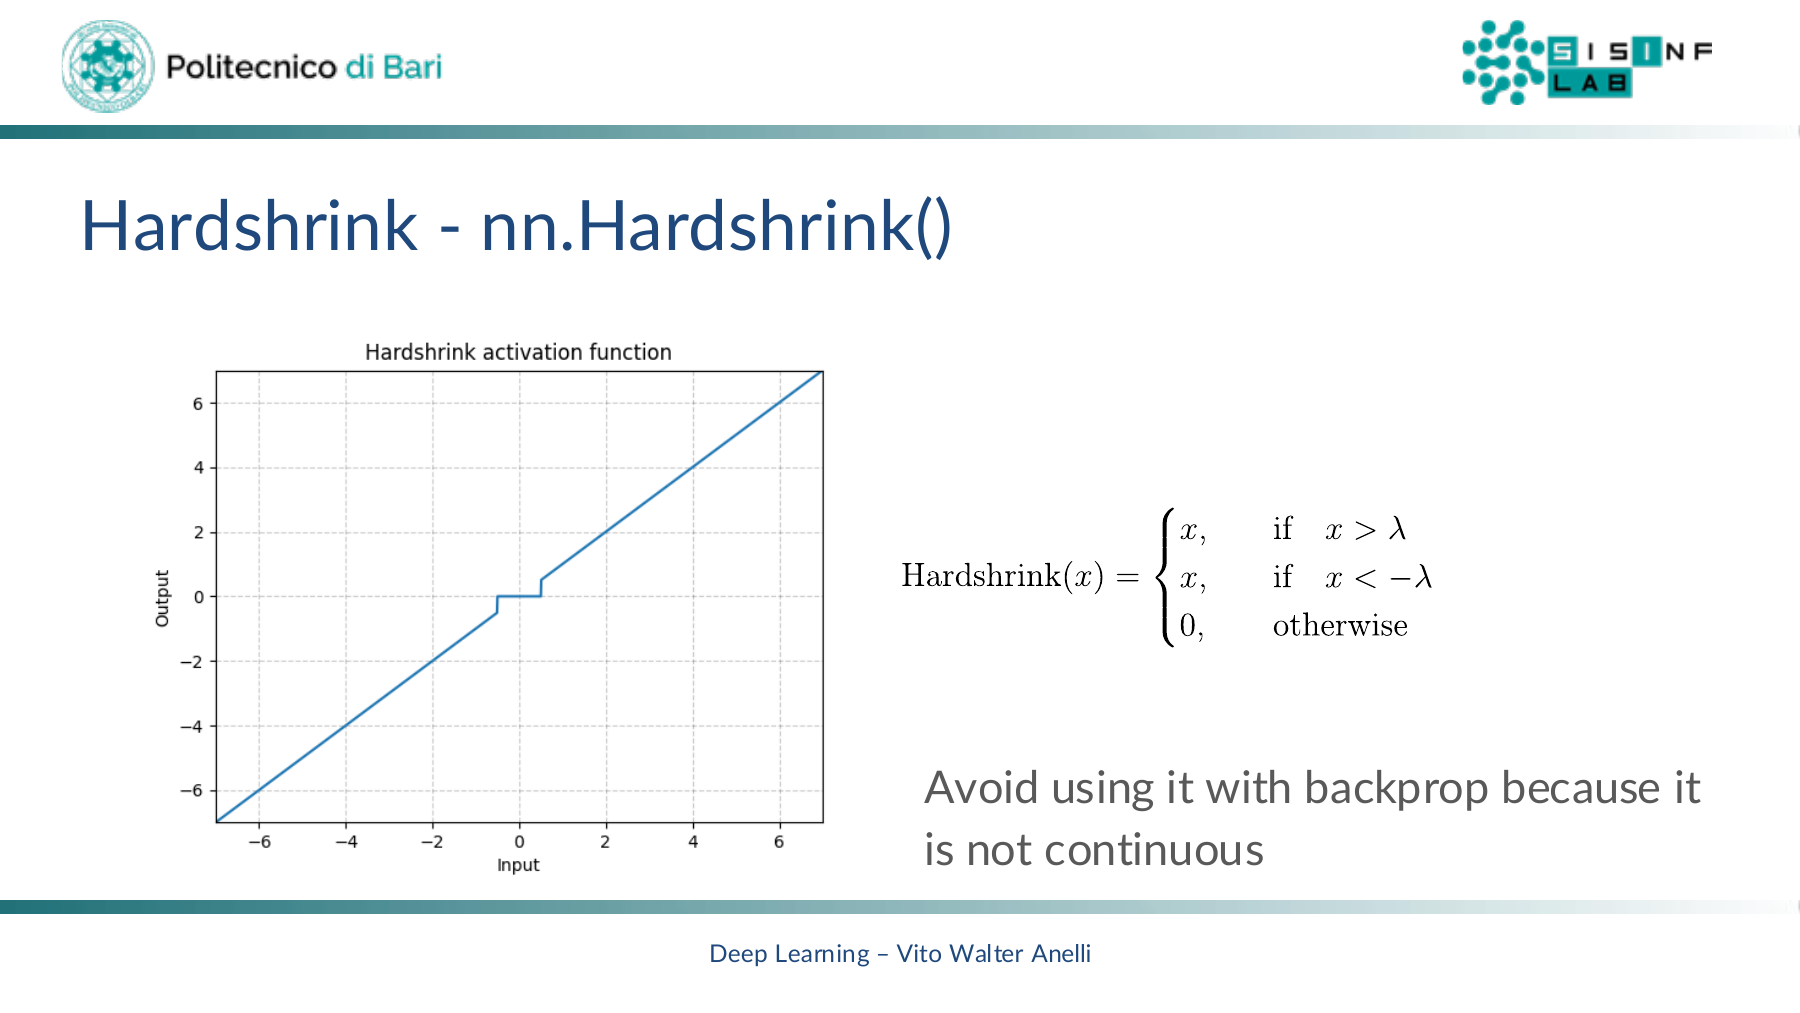
\includegraphics[width=0.85\linewidth]{figures/af03_hardshrink.png}
  \caption{Hardshrink: variante discontinua di Softshrink. La discontinuità in
           $x = \pm\lambda$ rende il gradiente non definito in quei punti, per
           cui \textbf{è sconsigliato l'uso con backpropagation}.
           Utilizzata in alcuni algoritmi di sparse coding fuori dal contesto
           delle reti neurali gradient-based.}
  \label{fig:hardshrink}
\end{figure}

%------------------------------------------------------------
\section{LogSigmoid -- \texttt{nn.LogSigmoid()}}
\label{sec:logsigmoid}

\begin{equation}
  \operatorname{LogSigmoid}(x) = \log\!\left(\frac{1}{1+\exp(-x)}\right).
\end{equation}

\begin{figure}[H]
  \centering
  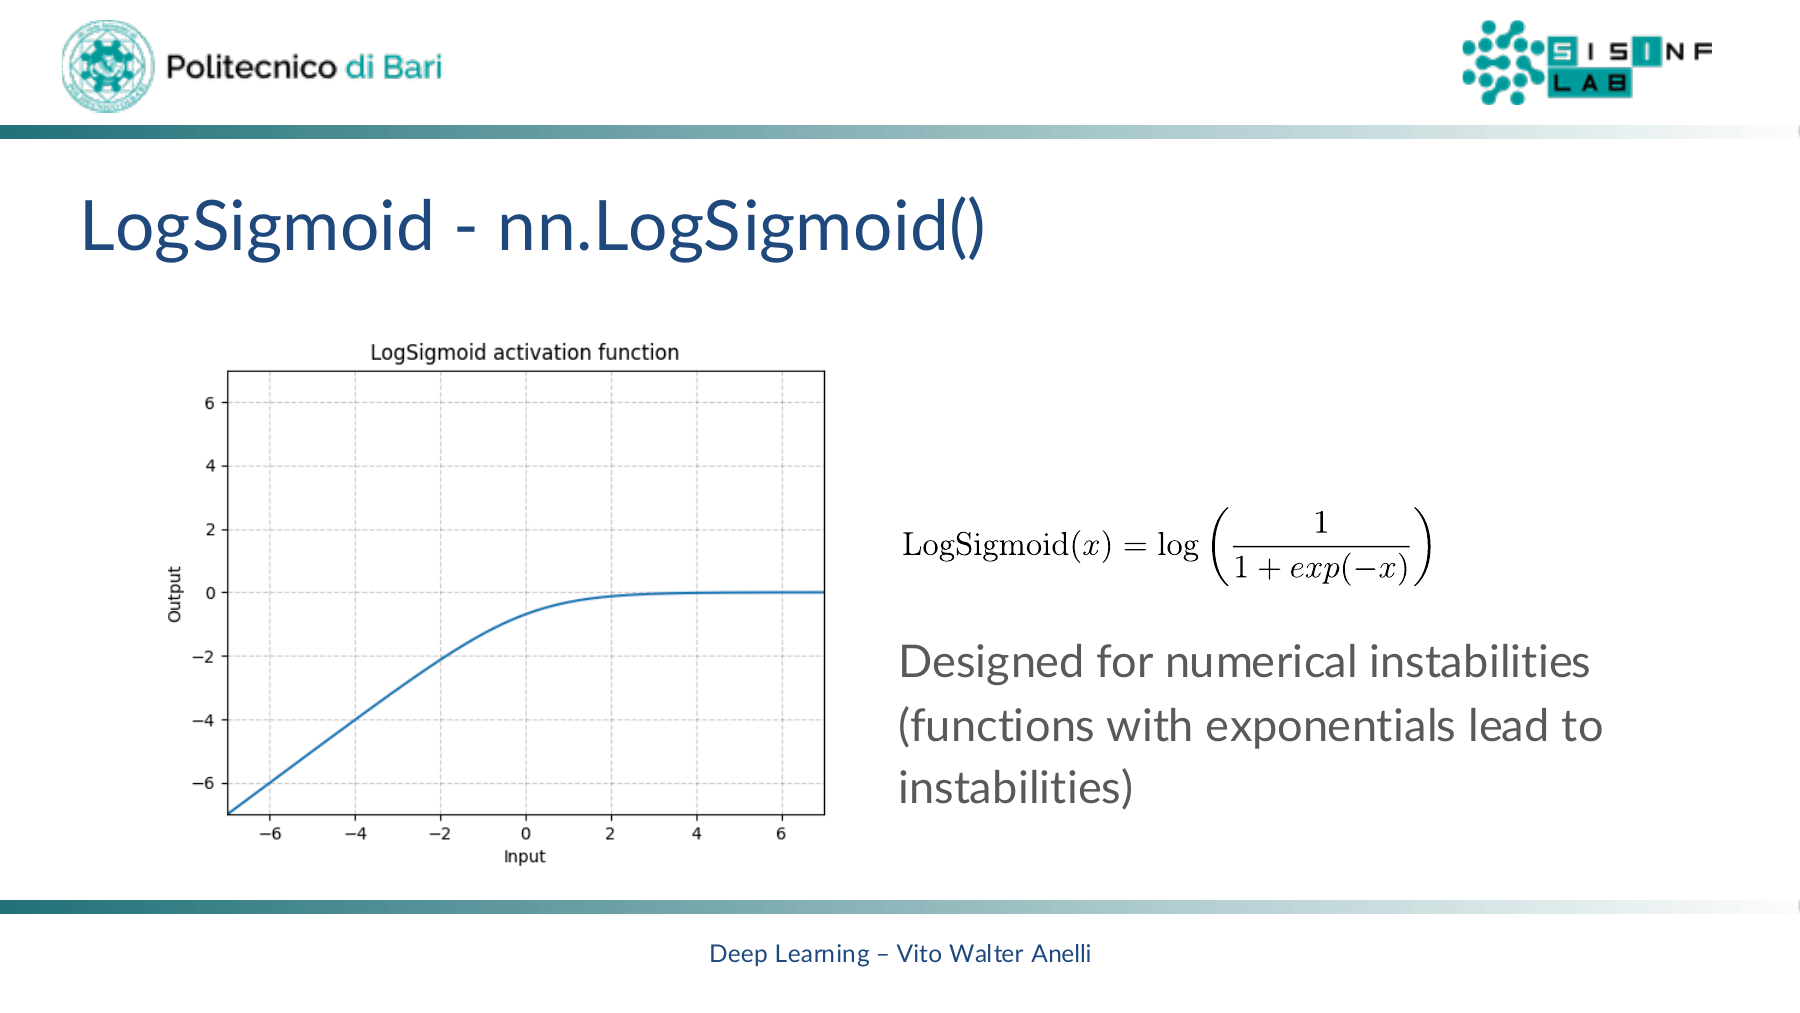
\includegraphics[width=0.85\linewidth]{figures/af03_logsigmoid.png}
  \caption{LogSigmoid: logaritmo della Sigmoid. Progettata per gestire le
           instabilità numeriche che emergono quando funzioni con esponenziali
           vengono composte (overflow/underflow). Usata prevalentemente nelle
           funzioni di costo, non come attivazione interna.}
  \label{fig:logsigmoid}
\end{figure}

%------------------------------------------------------------
\section{Funzioni Vettoriali: Softmin, Softmax, LogSoftmax}
\label{sec:softmax}

Le funzioni di questa sezione agiscono su \textbf{vettori interi}, trasformando
un vettore di scores in una distribuzione di probabilità. Non sono usate come
attivazioni interne, ma tipicamente nell'ultimo layer per compiti di
classificazione multiclasse.

\subsection{Softmin -- \texttt{nn.Softmin()}}
\label{subsec:softmin}

\begin{equation}
  \operatorname{Softmin}(x_i) = \frac{\exp(-x_i)}{\sum_j \exp(-x_j)}.
\end{equation}

\begin{figure}[H]
  \centering
  \includegraphics[width=0.72\linewidth]{figures/af03_softmin.png}
  \caption{Softmin: enfatizza i valori più \emph{piccoli} del vettore input.
           Per $x = [1,2,3]$ produce $[0{,}665,\, 0{,}245,\, 0{,}090]$:
           il valore più piccolo ($1$) riceve la probabilità maggiore.
           Raro in pratica; utile in contesti dove si vuole ``selezionare''
           il minimo in modo differenziabile.}
  \label{fig:softmin}
\end{figure}

\subsection{Soft(arg)max -- \texttt{nn.Softmax()}}
\label{subsec:softmax}

\begin{equation}
  \operatorname{Softmax}(x_i) = \frac{\exp(x_i)}{\sum_j \exp(x_j)}.
\end{equation}

\begin{figure}[H]
  \centering
  \includegraphics[width=0.72\linewidth]{figures/af03_softmax.png}
  \caption{Softmax: trasforma uno score vettoriale in una distribuzione di
           probabilità sommante a $1$. Enfatizza il valore più grande:
           per $x=[1,2,3]$ produce $[0{,}090,\, 0{,}245,\, 0{,}665]$.
           Amplifica le differenze tra i valori (\emph{winner-takes-all}).}
  \label{fig:softmax}
\end{figure}

\paragraph{Softmax come generalizzazione di Sigmoid.}
La Sigmoid è un caso speciale della Softmax per due classi.
Fissando $x_2 = 0$:

\begin{equation}
  z_1 = \frac{e^{x_1}}{e^{x_1} + e^{x_2}}
      \xrightarrow{x_2=0}
      \frac{e^{x_1}}{e^{x_1} + 1}
      = \frac{1}{1 + e^{-x_1}} = \sigma(x_1).
\end{equation}

\begin{figure}[H]
  \centering
  \includegraphics[width=0.72\linewidth]{figures/af03_softmax_relation_sigmoid.png}
  \caption{Derivazione della Sigmoid come caso speciale della Softmax a 2 classi.
           Questa relazione spiega perché la regressione logistica binaria
           (che usa Sigmoid) è un caso speciale della Softmax multiclasse.}
  \label{fig:softmax_relation_sigmoid}
\end{figure}

\subsection{LogSoft(arg)max -- \texttt{nn.LogSoftmax()}}
\label{subsec:logsoftmax}

\begin{equation}
  \operatorname{LogSoftmax}(x_i) = \log\!\left(\frac{\exp(x_i)}{\sum_j \exp(x_j)}\right).
\end{equation}

\begin{figure}[H]
  \centering
  \includegraphics[width=0.72\linewidth]{figures/af03_logsoftmax.png}
  \caption{LogSoftmax: usato principalmente nelle funzioni di costo (es.\ in
           combinazione con \texttt{nn.NLLLoss}) per evitare instabilità
           numeriche (overflow/underflow per esponenziali grandi) e la
           saturazione di valori in $0$ e $1$. Non è comune come attivazione
           interna.}
  \label{fig:logsoftmax}
\end{figure}

%------------------------------------------------------------
\section{Softmax e Cross-Entropy Loss}
\label{sec:softmax-crossentropy}

Nell'ultimo layer di un classificatore multiclasse, la Softmax viene accoppiata
alla \textbf{Cross-Entropy Loss}:

\begin{equation}
  \mathcal{L}_{\mathrm{CE}} = -\sum_i q_i \log(p_i),
\end{equation}
dove $q_i \in \{0,1\}$ è la label one-hot e $p_i = \operatorname{Softmax}(x_i)$.
Per un vettore one-hot, la somma collassa a un solo termine:

\begin{equation}
  \mathcal{L}_{\mathrm{CE}} = -\log\bigl(\operatorname{Softmax}(x_{\mathrm{corr}})\bigr),
\end{equation}
ossia si \emph{massimizza la probabilità assegnata alla classe corretta}
(o equivalentemente si minimizza il suo logaritmo negativo).

\begin{figure}[H]
  \centering
  \includegraphics[width=0.82\linewidth]{figures/af03_softmax_crossentropy.png}
  \caption{Softmax + Cross-Entropy Loss: il layer Softmax produce una distribuzione
           $[0{,}1,\ 0{,}2,\ 0{,}6,\ 0{,}1]$ mentre il target one-hot seleziona
           la classe 2 ($[0,1,0,0]$). La loss è $-\log(0{,}2)$. In pratica
           si usa \texttt{nn.CrossEntropyLoss} in PyTorch che fonde
           \texttt{LogSoftmax} e \texttt{NLLLoss} per stabilità numerica.}
  \label{fig:softmax_crossentropy}
\end{figure}

In PyTorch è raccomandato usare \texttt{nn.CrossEntropyLoss} anziché
\texttt{nn.Softmax} + \texttt{nn.NLLLoss} separatamente, perché la
formulazione unificata implementa il log-sum-exp trick che evita overflow
numerici \citep{bishop2024}.

%------------------------------------------------------------
\section{Guida Pratica alla Scelta}
\label{sec:practical-guide}

La scelta della funzione di attivazione dipende dal task, dalla profondità
della rete e dai requisiti computazionali. Le linee guida di \citet{bishop2024}
e del corso NYU-DL possono essere sintetizzate nella Tabella~\ref{tab:activation_guide}.

\begin{table}[H]
  \centering
  \caption{Guida pratica alla scelta della funzione di attivazione.}
  \label{tab:activation_guide}
  \small
  \begin{tabularx}{\linewidth}{l l l X}
    \toprule
    \textbf{Funzione} & \textbf{Output range} & \textbf{Gradiente} & \textbf{Uso tipico} \\
    \midrule
    ReLU       & $[0, +\infty)$                  & Non sat.\ (pos.) & Default hidden layer \\
    Leaky ReLU & $(-\infty,+\infty)$              & Non saturante    & ReLU con dead neurons \\
    PReLU      & $(-\infty,+\infty)$              & Apprendibile     & Quando LReLU è insufficiente \\
    ELU        & $(-\alpha, +\infty)$             & Non saturante    & Hidden, mean $\approx 0$ \\
    SELU       & $(\approx{-1{,}76}, +\infty)$   & Self-norm.       & Reti senza BatchNorm \\
    GELU       & $\approx(-0{,}17, +\infty)$     & Non mon.         & Transformer (BERT, GPT) \\
    Sigmoid    & $(0, 1)$                         & Saturante        & Output prob.\ binaria, gate \\
    Tanh       & $(-1, 1)$                        & Saturante        & RNN, output centrato \\
    Softmax    & $(0,1)^C$, $\sum=1$              & Vettoriale       & Output multiclasse \\
    \bottomrule
  \end{tabularx}
\end{table}

\paragraph{Raccomandazioni operative.}
\begin{enumerate}
  \item \textbf{Punto di partenza}: usare \textbf{ReLU} per i layer nascosti
        di MLP e CNN; è semplice, efficiente e funziona bene nella maggior parte
        dei casi.
  \item \textbf{Dead neurons}: se si osservano molti neuroni inattivi (output
        sempre zero), passare a \textbf{Leaky ReLU} o \textbf{ELU}.
  \item \textbf{Reti senza BatchNorm}: considerare \textbf{SELU}, che fornisce
        self-normalization automatica.
  \item \textbf{Transformer}: preferire \textbf{GELU}, che è la scelta standard
        in BERT, GPT-2/3 e modelli derivati.
  \item \textbf{Output layer}: usare \textbf{Sigmoid} per classificazione binaria,
        \textbf{Softmax} per multiclasse, nessuna attivazione (o ReLU/Softplus)
        per regressione con output positivo.
  \item \textbf{Loss function}: abbinare sempre \texttt{nn.CrossEntropyLoss}
        alla Softmax (fuse internamente con \texttt{LogSoftmax}) per stabilità
        numerica.
\end{enumerate}

%------------------------------------------------------------
\section{Riepilogo}
\label{sec:summary-ch3}

\begin{center}
\small
\begin{tabularx}{\linewidth}{l l X}
  \toprule
  \textbf{Problema} & \textbf{Causa} & \textbf{Soluzione} \\
  \midrule
  Vanishing gradient  & Saturazione Sigmoid/Tanh  & ReLU, ELU, GELU \\
  Dead neurons        & ReLU $=0$ per input neg.  & LReLU, PReLU, ELU \\
  Output non centrato & ReLU $\geq 0$ sempre      & ELU, SELU, BatchNorm \\
  Instabilità num.    & Exp.\ overflow in Softmax & LogSoftmax, CrossEntropyLoss \\
  Parametri extra     & PReLU: $a$ apprendibile   & Beneficio: adattività \\
  Non monotonicità    & GELU ha un ``dip''         & Proprietà regolatrice \\
  \bottomrule
\end{tabularx}
\end{center}

Le funzioni di attivazione rappresentano uno degli assi portanti
dell'ingegneria delle reti neurali: la scelta sbagliata può precludere
l'apprendimento nei layer profondi (vanishing gradient), mentre la scelta
giusta velocizza la convergenza e migliora la generalizzazione.
Il consenso attuale nella letteratura è di usare ReLU o le sue varianti
non saturanti come default, riservando Sigmoid e Tanh ai casi in cui
la struttura del problema lo impone (output probabilistici, meccanismi
di gating, reti ricorrenti).

% ...

%============================================================
% BIBLIOGRAFIA
%============================================================
\bibliographystyle{plainnat}
\bibliography{bibliography/refs}

\end{document}
